\documentclass[conference]{IEEEtran}
\usepackage{cite}
\usepackage{amsmath,amssymb,amsfonts}
\usepackage{algorithmic}
\usepackage{graphicx}
\usepackage{textcomp}
\usepackage{hyperref}
\usepackage{xcolor}
\usepackage{tikz}
\usepackage{siunitx}
\usepackage{booktabs}
\usepackage{multirow}
\usepackage{listings}
\usepackage[utf8]{inputenc}
\usepackage{pgfplots}
\newcommand{\NA}{---}
\usetikzlibrary{angles, quotes, decorations.markings, positioning}
\def\BibTeX{{\rm B\kern-.05em{\sc i\kern-.025em b}\kern-.08em
    T\kern-.1667em\lower.7ex\hbox{E}\kern-.125emX}}
\usepgfplotslibrary{groupplots,dateplot}
\usetikzlibrary{patterns,shapes.arrows}
\pgfplotsset{compat=newest}


\begin{document}

\title{A Study of Standing Waves in a Tube}

\author{\IEEEauthorblockN{Marko Vejnovi\'{c}}
\IEEEauthorblockA{\textit{Department of Electrical and Computer Engineering} \\
\textit{Northwestern University}\\
Evanston, Illinois \\
markovejnovic2023@u.northwestern.edu}
}

\maketitle

\begin{abstract}
    This paper outlines the research conducted in the field of tube harmonics.
    The relationship between tube length and the resonant wavelength was
    investigated, as well as the speed of sound. The already well established
    relationship between the tube length and the resonant wavelength was
    confirmed with high certainty, and the speed of sound was measured to be
    341.75 m/s.
\end{abstract}

\section{Introduction}

A tube allows for the formation of standing pressure waves. Given a sinusoidal
pressure wave entering a tube with a closed end, the pressure wave will be
reflected at the back wall of the tube.

For the formation of a standing wave, there must be an anti-node at the back
wall of the tube and a node at the open end, as shown in Fig.
\ref{fig:tube-diagram}. This results in a requirement for standing waves:
\begin{equation}\label{eqn:base}
    \lambda = \frac{4L}{2n - 1}
\end{equation}

\begin{figure}[b!]
    \centering
    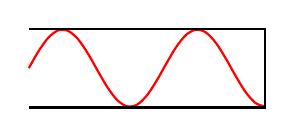
\begin{tikzpicture}
        \draw[thick, red, domain=0:3, smooth] plot ({\x}, {0.49 * sin(3.6652 * \x r) - 0.5});
        \draw[thick] (0,0) -- (3,0) -- (3,-1) -- (0,-1);
    \end{tikzpicture}
    \caption{Standing Wave in a Closed Tube}
    \label{fig:tube-diagram}
\end{figure}

Finally, it is worth noting that \eqref{eqn:base} is equivalent to:
\begin{equation}\label{eqn:base-freq}
    \frac{\nu}{f} = \frac{4L}{2n - 1}
\end{equation}

The aim of this research was to empirically test whether \eqref{eqn:base} is a
good model for the resonance in a tube, as well as determine the speed of sound
from \eqref{eqn:base-freq}.

\section{Method}

This section outlines the apparatus used and the procedure.

\subsection{Apparatus}

The experiment setup was as follows. A measuring cylinder was set on a flat
table. Near its open end an \textit{Audio Technica AT2021}\cite{at2021}
monodirectional microphone was placed. The microphone was driven by a
\textit{Focusrite Scarlett Solo 2}\cite{focusrite} into a computer. The
cylinder was disturbed by a wind stream, induced by simply blowing over its
top. A block diagram is given in Fig. \ref{fig:block-diagram}. The cylinder
length was controlled by adding water to it. The device used for measuring
length was a tape meter with an uncertainty of $\pm 0.5\si{mm}$.
\textit{Audacity}\cite{audacity} was used for recording the wave.

The temperature, at the time of measuring was around $\ang{15}C$ and the
humidity was around $40\%$. This yields a wavespeed of \cite{sostbl}:
\begin{equation*}
    \nu = 340.8 \si{\frac{m}{s}}
\end{equation*}

\begin{figure}[b!]
    \centering
    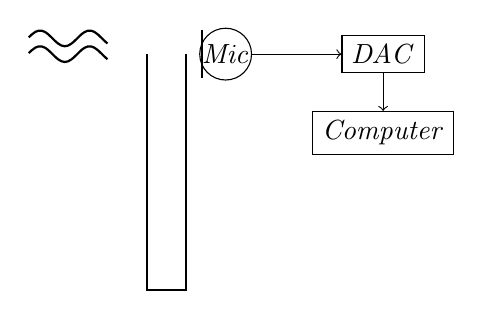
\begin{tikzpicture}
        \node[draw, circle, inner sep=0.1pt, outer sep=0.1pt] (Mic) {\textit{Mic}};
        \node[draw] (DAC) at (2, 0) {\textit{DAC}};
        \node[draw] (Computer) at (2, -1) {\textit{Computer}};
        \draw[->] (Mic) edge (DAC);
        \draw[->] (DAC) edge (Computer);
        \draw[thick] (-0.3,-0.3) -- (-0.3,0.3);
        \draw[thick] (-0.5,0) -- (-0.5,-3) -- (-1,-3) -- (-1,0);
        \draw[thick, domain=-2.5:-1.5, smooth] plot ({\x}, {0.1 * sin(10 * \x r)});
        \draw[thick, domain=-2.5:-1.5, smooth] plot ({\x}, {0.1 * sin(10 * \x r) + 0.2});
    \end{tikzpicture}
    \caption{The Experimental Setup Block Diagram}
    \label{fig:block-diagram}
\end{figure}

\subsection{Procedure}

For each target tube length, water was added to the measuring cylinder to reach
the target length. The tube length was measured. Recording was initialized on
the computer and a stream was blown over the tube opening. After blowing was
done, the recording was saved into a \texttt{wav} file.

\section{Results}

The raw waveforms are available at \cite{raw-waveforms}.

\subsection{Data Processing}

The positive Fourier transform of the waveform was found. The magnitude of the
Fourier transform was normalized and the peaks were identified. This was all
done with \textit{python}\cite{python}, \textit{numpy}\cite{numpy},
\textit{scipy}\cite{scipy} and \textit{matplotlib}\cite{matplotlib}, available
at \cite{raw-waveforms}.

An example of peak identification is given in Fig. \ref{fig:peaks-identified}.

\begin{figure}[b!]
    \centering
    % This file was created by tikzplotlib v0.9.8.
\begin{tikzpicture}

\definecolor{color0}{rgb}{0.12156862745098,0.466666666666667,0.705882352941177}
\definecolor{color1}{rgb}{1,0.498039215686275,0.0549019607843137}

\begin{axis}[
legend cell align={left},
legend style={fill opacity=0.8, draw opacity=1, text opacity=1, draw=white!80!black},
tick align=outside,
tick pos=left,
x grid style={white!69.0196078431373!black},
xlabel={Frequency [Hz]},
xmin=0, xmax=4500,
xtick style={color=black},
xtick={0,500,1000,1500,2000,2500,3000,3500,4000,4500},
xticklabels={
  \(\displaystyle {0}\),
  \(\displaystyle {500}\),
  \(\displaystyle {1000}\),
  \(\displaystyle {1500}\),
  \(\displaystyle {2000}\),
  \(\displaystyle {2500}\),
  \(\displaystyle {3000}\),
  \(\displaystyle {3500}\),
  \(\displaystyle {4000}\),
  \(\displaystyle {4500}\)
},
y grid style={white!69.0196078431373!black},
ylabel={Normalized Magnitude},
ymin=-0.0499988657481308, ymax=1.04999994598801,
ytick style={color=black},
ytick={-0.2,0,0.2,0.4,0.6,0.8,1,1.2},
yticklabels={
  \(\displaystyle {−0.2}\),
  \(\displaystyle {0.0}\),
  \(\displaystyle {0.2}\),
  \(\displaystyle {0.4}\),
  \(\displaystyle {0.6}\),
  \(\displaystyle {0.8}\),
  \(\displaystyle {1.0}\),
  \(\displaystyle {1.2}\)
}
]
\addplot [line width=0.28pt, color0]
table {%
0 0.0106230974197388
0.175423264503479 0.0017019510269165
0.350846529006958 0.00193512439727783
0.526269674301147 0.00157678127288818
0.877116203308105 0.00213289260864258
1.05253946781158 0.00723803043365479
1.22796273231506 0.00726890563964844
1.40338599681854 0.0121959447860718
1.57880914211273 0.0197590589523315
1.75423240661621 0.0105198621749878
1.92965567111969 0.0104789733886719
2.10507893562317 0.015129566192627
2.28050208091736 0.0171079635620117
2.45592546463013 0.0149955749511719
2.63134860992432 0.018407940864563
2.80677199363708 0.000919699668884277
2.98219513893127 0.0326958894729614
3.15761828422546 0.0208820104598999
3.33304166793823 0.0540566444396973
3.50846481323242 0.090999960899353
3.68388819694519 0.0236133337020874
3.85931134223938 0.0732431411743164
4.03473472595215 0.0850739479064941
4.21015787124634 0.0621860027313232
4.38558101654053 0.146780848503113
4.56100416183472 0.264586448669434
4.73642778396606 0.260933399200439
4.91185092926025 0.310449004173279
5.08727407455444 0.235259413719177
5.26269721984863 0.468083381652832
5.43812036514282 0.534226298332214
5.61354398727417 0.670310974121094
5.78896713256836 0.604231357574463
5.96439027786255 0.21981143951416
6.13981342315674 0.634318828582764
6.31523656845093 0.656377792358398
6.49066019058228 0.960771322250366
6.66608333587646 0.875787615776062
6.84150648117065 0.626562714576721
7.01692962646484 0.293977737426758
7.19235277175903 0.93100380897522
7.36777639389038 0.61983335018158
7.54319953918457 0.364647626876831
7.71862268447876 0.830004572868347
7.89404582977295 0.321385860443115
8.0694694519043 0.249122738838196
8.24489212036133 0.276052951812744
8.42031574249268 0.239797472953796
8.59573936462402 0.155393123626709
8.77116203308105 0.318557739257812
8.9465856552124 0.256143927574158
9.12200832366943 0.355341672897339
9.29743194580078 0.0653793811798096
9.47285556793213 0.280732154846191
9.64827823638916 0.237177968025208
9.82370185852051 0.365675330162048
9.99912452697754 0.53545343875885
10.1745481491089 0.588282823562622
10.3499717712402 0.357262492179871
10.5253944396973 0.22050404548645
10.7008180618286 0.282786846160889
10.8762407302856 0.213457226753235
11.051664352417 0.197960615158081
11.2270879745483 0.117655396461487
11.4025106430054 0.118625998497009
11.5779342651367 0.0875091552734375
11.7533569335938 0.45073413848877
11.9287805557251 0.561799645423889
12.1042041778564 0.357775688171387
12.2796268463135 0.179967403411865
12.4550504684448 0.0508376359939575
12.6304731369019 0.1449054479599
12.8058967590332 0.239840269088745
12.9813203811646 0.194587588310242
13.1567430496216 0.121852159500122
13.3321666717529 0.00958085060119629
13.50758934021 0.115243554115295
13.6830129623413 0.0578885078430176
13.8584365844727 0.123992681503296
14.0338592529297 0.161899447441101
14.209282875061 0.240116119384766
14.3847055435181 0.278335571289062
14.5601291656494 0.117376804351807
14.7355527877808 0.105934143066406
14.9109754562378 0.217289924621582
15.0863990783691 0.14927339553833
15.2618217468262 0.0400323867797852
15.4372453689575 0.102799654006958
15.6126689910889 0.0463501214981079
15.7880916595459 0.0808813571929932
15.9635152816772 0.144228100776672
16.1389389038086 0.0653755664825439
16.3143615722656 0.104652285575867
16.4897842407227 0.184061050415039
16.6652088165283 0.17836332321167
16.8406314849854 0.14145815372467
17.0160541534424 0.109998106956482
17.191478729248 0.0277473926544189
17.3669013977051 0.051522970199585
17.5423240661621 0.0768364667892456
17.7177467346191 0.106152296066284
17.8931713104248 0.153927564620972
18.0685939788818 0.133681535720825
18.2440166473389 0.222213745117188
18.4194412231445 0.222383975982666
18.5948638916016 0.191478848457336
18.7702865600586 0.216640472412109
18.9457111358643 0.17839789390564
19.1211338043213 0.0926909446716309
19.2965564727783 0.0732990503311157
19.4719791412354 0.116793751716614
19.647403717041 0.0959763526916504
19.822826385498 0.0942951440811157
19.9982490539551 0.116989016532898
20.1736736297607 0.12332010269165
20.3490962982178 0.103098392486572
20.5245189666748 0.153708338737488
20.6999435424805 0.155780434608459
20.8753662109375 0.0614684820175171
21.0507888793945 0.0575131177902222
21.2262115478516 0.102590203285217
21.4016361236572 0.100388526916504
21.5770587921143 0.118284344673157
21.7524814605713 0.129637241363525
21.927906036377 0.1064612865448
22.103328704834 0.105982184410095
22.278751373291 0.0466779470443726
22.4541759490967 0.0576287508010864
22.6295986175537 0.0472899675369263
22.8050212860107 0.0297044515609741
22.9804439544678 0.0358040332794189
23.1558685302734 0.069823145866394
23.3312911987305 0.0896356105804443
23.5067138671875 0.0394796133041382
23.6821384429932 0.0486173629760742
23.8575611114502 0.0888963937759399
24.0329837799072 0.0751990079879761
24.2084083557129 0.0157501697540283
24.3838310241699 0.0797727108001709
24.559253692627 0.0769784450531006
24.7346782684326 0.0749472379684448
24.9101009368896 0.0760407447814941
25.0855236053467 0.0573843717575073
25.2609462738037 0.0612924098968506
25.4363708496094 0.0803545713424683
25.6117935180664 0.0777024030685425
25.7872161865234 0.102316856384277
25.9626407623291 0.0594408512115479
26.1380634307861 0.0820708274841309
26.3134860992432 0.0604181289672852
26.4889106750488 0.0439848899841309
26.6643333435059 0.0490703582763672
26.8397560119629 0.0207793712615967
27.0151786804199 0.0259310007095337
27.1906032562256 0.0414756536483765
27.3660259246826 0.0995428562164307
27.5414485931396 0.123655915260315
27.7168731689453 0.0709888935089111
27.8922958374023 0.0764116048812866
28.0677185058594 0.08819580078125
28.243143081665 0.0809527635574341
28.4185657501221 0.00817060470581055
28.5939884185791 0.0411317348480225
28.7694110870361 0.0150094032287598
28.9448356628418 0.0621044635772705
29.1202583312988 0.0856771469116211
29.2956809997559 0.102457880973816
29.4711055755615 0.0341882705688477
29.6465282440186 0.0605592727661133
29.8219509124756 0.0547333955764771
29.9973754882812 0.0682047605514526
30.1727981567383 0.06215500831604
30.3482208251953 0.00957822799682617
30.5236434936523 0.044751763343811
30.699068069458 0.0510528087615967
30.874490737915 0.0725729465484619
31.0499134063721 0.074852466583252
31.2253379821777 0.00829529762268066
31.4007606506348 0.0914793014526367
31.5761833190918 0.0269503593444824
31.7516078948975 0.0868438482284546
31.9270305633545 0.137314558029175
32.1024551391602 0.086396336555481
32.2778778076172 0.107100248336792
32.4533004760742 0.0922222137451172
32.6287231445312 0.0845922231674194
32.8041458129883 0.0823637247085571
32.9795684814453 0.0987246036529541
33.1549911499023 0.0518325567245483
33.3304176330566 0.0555100440979004
33.5058403015137 0.0403068065643311
33.6812629699707 0.0275415182113647
33.8566856384277 0.0331418514251709
34.0321083068848 0.0598270893096924
34.2075309753418 0.00504481792449951
34.3829574584961 0.0653051137924194
34.5583801269531 0.16742742061615
34.7338027954102 0.139542102813721
34.9092254638672 0.0653592348098755
35.0846481323242 0.106513500213623
35.2600708007812 0.0519888401031494
35.4354934692383 0.0769625902175903
35.6109199523926 0.0553470849990845
35.7863426208496 0.11929452419281
35.9617652893066 0.0655449628829956
36.1371879577637 0.13106369972229
36.3126106262207 0.0298757553100586
36.4880332946777 0.0295482873916626
36.6634559631348 0.106348276138306
36.8388824462891 0.103750467300415
37.0143051147461 0.0819224119186401
37.1897277832031 0.110424518585205
37.3651504516602 0.0084148645401001
37.5405731201172 0.0504711866378784
37.7159957885742 0.187794327735901
37.8914222717285 0.100523471832275
38.0668449401855 0.141906023025513
38.2422676086426 0.033271312713623
38.4176902770996 0.0198191404342651
38.5931129455566 0.0521842241287231
38.7685356140137 0.0648179054260254
38.9439582824707 0.0130789279937744
39.119384765625 0.0304737091064453
39.294807434082 0.0620248317718506
39.6456527709961 0.152269005775452
39.8210754394531 0.165894269943237
39.9964981079102 0.103377461433411
40.1719245910645 0.0589549541473389
40.3473472595215 0.116724014282227
40.5227699279785 0.0324296951293945
40.6981925964355 0.0723750591278076
40.8736152648926 0.0263392925262451
41.0490379333496 0.0512653589248657
41.2244606018066 0.057904839515686
41.3998870849609 0.0731391906738281
41.575309753418 0.115243315696716
41.750732421875 0.0562782287597656
41.926155090332 0.0578913688659668
42.1015777587891 0.0372872352600098
42.2770004272461 0.0527215003967285
42.4524230957031 0.0509227514266968
42.6278495788574 0.15692150592804
42.8032722473145 0.0752605199813843
42.9786949157715 0.121166229248047
43.1541175842285 0.0524333715438843
43.3295402526855 0.082686185836792
43.5049629211426 0.144798278808594
43.6803894042969 0.0424129962921143
43.8558120727539 0.0217442512512207
44.0312347412109 0.0715104341506958
44.206657409668 0.084764838218689
44.382080078125 0.118696928024292
44.557502746582 0.148467063903809
44.7329254150391 0.040357232093811
44.9083518981934 0.0340477228164673
45.0837745666504 0.101593375205994
45.2591972351074 0.0782822370529175
45.4346199035645 0.0686063766479492
45.6100425720215 0.0818538665771484
45.7854652404785 0.052815318107605
45.9608879089355 0.0420999526977539
46.1363143920898 0.0506715774536133
46.3117370605469 0.0452312231063843
46.4871597290039 0.0596185922622681
46.6625823974609 0.0285172462463379
46.838005065918 0.0393378734588623
47.013427734375 0.00994479656219482
47.1888542175293 0.0428429841995239
47.3642768859863 0.0712933540344238
47.5396995544434 0.0821666717529297
47.7151222229004 0.0914782285690308
47.8905448913574 0.0861338376998901
48.0659675598145 0.105543613433838
48.2413902282715 0.0324392318725586
48.4168167114258 0.0694104433059692
48.5922393798828 0.0950164794921875
48.7676620483398 0.0486997365951538
48.9430847167969 0.0651758909225464
49.1185073852539 0.0943719148635864
49.2939300537109 0.0563387870788574
49.4693565368652 0.0616210699081421
49.6447792053223 0.0358593463897705
49.8202018737793 0.0654829740524292
49.9956245422363 0.030553936958313
50.1710472106934 0.025763988494873
50.3464698791504 0.021728515625
50.5218925476074 0.0123851299285889
50.6973190307617 0.0549157857894897
50.8727416992188 0.0995895862579346
51.0481643676758 0.107848405838013
51.2235870361328 0.120568037033081
51.3990097045898 0.0983989238739014
51.5744323730469 0.0683077573776245
51.7498550415039 0.0465906858444214
51.9252815246582 0.0307959318161011
52.1007041931152 0.0224781036376953
52.2761268615723 0.0731109380722046
52.4515495300293 0.0812876224517822
52.6269721984863 0.0654604434967041
52.8023948669434 0.0241904258728027
52.9778213500977 0.0560766458511353
53.1532440185547 0.0657457113265991
53.3286666870117 0.0162841081619263
53.5040893554688 0.0586272478103638
53.6795120239258 0.0601924657821655
53.8549346923828 0.0740399360656738
54.0303573608398 0.0694220066070557
54.2057838439941 0.0834454298019409
54.3812065124512 0.0940386056900024
54.5566291809082 0.0943912267684937
54.7320518493652 0.0903934240341187
54.9074745178223 0.0606645345687866
55.0828971862793 0.0636681318283081
55.2583198547363 0.0464930534362793
55.4337463378906 0.0561178922653198
55.6091690063477 0.104472398757935
55.7845916748047 0.0798331499099731
55.9600143432617 0.0633617639541626
56.1354370117188 0.0489016771316528
56.3108596801758 0.0287917852401733
56.4862861633301 0.036848783493042
56.6617088317871 0.0479755401611328
56.8371315002441 0.044089674949646
57.0125541687012 0.0557785034179688
57.1879768371582 0.0279339551925659
57.3633995056152 0.0506666898727417
57.5388221740723 0.0873948335647583
57.7142486572266 0.0511032342910767
57.8896713256836 0.0434775352478027
58.0650939941406 0.120598554611206
58.2405166625977 0.0979264974594116
58.4159393310547 0.052384614944458
58.5913619995117 0.0547546148300171
58.7667846679688 0.0241742134094238
58.942211151123 0.0210353136062622
59.1176338195801 0.010403037071228
59.2930564880371 0.0399459600448608
59.4684791564941 0.0742006301879883
59.6439018249512 0.0771058797836304
59.8193244934082 0.00855004787445068
59.9947509765625 0.02821946144104
60.1701736450195 0.0528712272644043
60.3455963134766 0.00401031970977783
60.5210189819336 0.0301487445831299
60.6964416503906 0.0719932317733765
60.8718643188477 0.0169287919998169
61.0472869873047 0.0713872909545898
61.222713470459 0.0970338582992554
61.398136138916 0.0391335487365723
61.573558807373 0.0703680515289307
61.7489814758301 0.0722500085830688
61.9244041442871 0.0389190912246704
62.0998268127441 0.0211082696914673
62.2752532958984 0.0319148302078247
62.4506759643555 0.0691753625869751
62.6260986328125 0.0522361993789673
62.8015213012695 0.0693947076797485
62.9769439697266 0.054729700088501
63.1523666381836 0.0550076961517334
63.3277893066406 0.0230094194412231
63.5032157897949 0.0595905780792236
63.678638458252 0.0565787553787231
63.854061126709 0.0481582880020142
64.0294876098633 0.0325406789779663
64.2049102783203 0.0343029499053955
64.3803329467773 0.083959698677063
64.5557556152344 0.0758056640625
64.7311782836914 0.0339937210083008
64.9066009521484 0.0768054723739624
65.0820236206055 0.0278544425964355
65.2574462890625 0.0268900394439697
65.4328689575195 0.0532921552658081
65.6082916259766 0.0250967741012573
65.7837142944336 0.0195329189300537
65.9591369628906 0.0164415836334229
66.1345596313477 0.0161020755767822
66.3099822998047 0.0282115936279297
66.4854125976562 0.0559349060058594
66.6608352661133 0.052177906036377
66.8362579345703 0.0344678163528442
67.0116806030273 0.00840771198272705
67.1871032714844 0.027667760848999
67.3625259399414 0.0659449100494385
67.5379486083984 0.0840559005737305
67.7133712768555 0.086575984954834
67.8887939453125 0.0600532293319702
68.0642166137695 0.0478560924530029
68.2396392822266 0.0507135391235352
68.4150619506836 0.0410207509994507
68.5904846191406 0.0199980735778809
68.7659149169922 0.003662109375
68.9413375854492 0.0141381025314331
69.1167602539062 0.0228986740112305
69.2921829223633 0.0323846340179443
69.4676055908203 0.0280371904373169
69.6430282592773 0.0096973180770874
69.8184509277344 0.0157104730606079
69.9938735961914 0.0704195499420166
70.1692962646484 0.0862784385681152
70.3447189331055 0.0247209072113037
70.5201416015625 0.0694377422332764
70.6955642700195 0.113635063171387
70.8709869384766 0.0447573661804199
71.0464172363281 0.0431749820709229
71.2218399047852 0.073023796081543
71.3972625732422 0.04884934425354
71.5726852416992 0.0733485221862793
71.7481079101562 0.0800771713256836
71.9235305786133 0.0744669437408447
72.0989532470703 0.0624964237213135
72.2743759155273 0.0329478979110718
72.4497985839844 0.0349752902984619
72.6252212524414 0.0417311191558838
72.8006439208984 0.0353566408157349
72.9760665893555 0.0422230958938599
73.1514892578125 0.0696173906326294
73.3269119262695 0.0735692977905273
73.5023422241211 0.0577219724655151
73.6777648925781 0.0424542427062988
73.8531875610352 0.0239286422729492
74.0286102294922 0.0251767635345459
74.2040328979492 0.0315288305282593
74.5548782348633 0.06226646900177
74.7303009033203 0.0299280881881714
74.9057235717773 0.0600658655166626
75.0811462402344 0.0492093563079834
75.2565689086914 0.0246995687484741
75.4319915771484 0.0292052030563354
75.6074142456055 0.0125426054000854
75.782844543457 0.0314900875091553
75.9582672119141 0.0366041660308838
76.1336898803711 0.073743462562561
76.3091125488281 0.0497043132781982
76.4845352172852 0.0209972858428955
76.6599578857422 0.0524494647979736
76.8353805541992 0.0376570224761963
77.0108032226562 0.0162702798843384
77.1862258911133 0.0205847024917603
77.3616485595703 0.0620672702789307
77.5370712280273 0.0539827346801758
77.7124938964844 0.0851286649703979
77.8879165649414 0.102242112159729
78.063346862793 0.065449595451355
78.23876953125 0.0275263786315918
78.414192199707 0.00594198703765869
78.5896148681641 0.0254169702529907
78.7650375366211 0.036384105682373
78.9404602050781 0.0559117794036865
79.1158828735352 0.058340311050415
79.2913055419922 0.0331090688705444
79.4667282104492 0.0221714973449707
79.6421508789062 0.049053430557251
79.8175735473633 0.0263617038726807
79.9929962158203 0.0375649929046631
80.1684188842773 0.054481029510498
80.3438491821289 0.0331000089645386
80.5192718505859 0.0524497032165527
80.694694519043 0.0502043962478638
80.8701171875 0.0326974391937256
81.045539855957 0.0477886199951172
81.2209625244141 0.0304887294769287
81.3963851928711 0.0110595226287842
81.5718078613281 0.0285537242889404
81.7472305297852 0.0358821153640747
81.9226531982422 0.00894272327423096
82.0980758666992 0.0380699634552002
82.2734985351562 0.0606523752212524
82.4489212036133 0.0367072820663452
82.6243438720703 0.0282924175262451
82.7997741699219 0.0736082792282104
82.9751968383789 0.0768589973449707
83.1506195068359 0.0370053052902222
83.326042175293 0.035503625869751
83.50146484375 0.0347425937652588
83.676887512207 0.0397285223007202
83.8523101806641 0.0477970838546753
84.0277328491211 0.0569659471511841
84.2031555175781 0.0856902599334717
84.3785781860352 0.0766113996505737
84.5540008544922 0.0474498271942139
84.7294235229492 0.0311466455459595
84.9048461914062 0.0443284511566162
85.0802764892578 0.0964566469192505
85.2556991577148 0.122283697128296
85.4311218261719 0.0963680744171143
85.6065444946289 0.0614204406738281
85.7819671630859 0.070067286491394
85.957389831543 0.0629866123199463
86.1328125 0.0300089120864868
86.308235168457 0.0221141576766968
86.4836578369141 0.0524376630783081
86.6590805053711 0.0560898780822754
86.8345031738281 0.0079113245010376
87.0099258422852 0.0695867538452148
87.1853485107422 0.0956829786300659
87.3607788085938 0.054507851600647
87.5362014770508 0.0156904458999634
87.7116241455078 0.0319329500198364
87.8870468139648 0.0141055583953857
88.2378921508789 0.0902938842773438
88.4133148193359 0.0875656604766846
88.588737487793 0.0675218105316162
88.76416015625 0.0414321422576904
88.939582824707 0.0212864875793457
89.1150054931641 0.0146548748016357
89.2904281616211 0.0596444606781006
89.4658508300781 0.0989712476730347
89.6412811279297 0.106363773345947
89.8167037963867 0.0553464889526367
89.9921264648438 0.0443875789642334
90.1675491333008 0.0427595376968384
90.3429718017578 0.00780379772186279
90.5183944702148 0.0133509635925293
90.6938171386719 0.0181816816329956
90.8692398071289 0.0678142309188843
91.0446624755859 0.0832403898239136
91.220085144043 0.0581024885177612
91.3955078125 0.0655981302261353
91.570930480957 0.059456467628479
91.7463531494141 0.0233825445175171
91.9217758178711 0.0527611970901489
92.0972061157227 0.094687819480896
92.2726287841797 0.075980544090271
92.4480514526367 0.0224264860153198
92.6234741210938 0.0225422382354736
92.7988967895508 0.0198876857757568
92.9743194580078 0.0176539421081543
93.1497421264648 0.0212968587875366
93.3251647949219 0.0139836072921753
93.5005874633789 0.0347371101379395
93.6760101318359 0.0602716207504272
93.851432800293 0.0357750654220581
94.02685546875 0.0299544334411621
94.202278137207 0.059755802154541
94.3777084350586 0.0434025526046753
94.5531311035156 0.0229884386062622
94.7285537719727 0.0642549991607666
94.9039764404297 0.111397743225098
95.0793991088867 0.117708086967468
95.2548217773438 0.0737740993499756
95.4302444458008 0.0459071397781372
95.6056671142578 0.0315848588943481
95.7810897827148 0.0624053478240967
95.9565124511719 0.0802441835403442
96.1319351196289 0.0805822610855103
96.3073577880859 0.0542398691177368
96.482780456543 0.0212323665618896
96.6582107543945 0.00728356838226318
96.8336334228516 0.00607287883758545
97.0090560913086 0.0622978210449219
97.1844787597656 0.0885798931121826
97.3599014282227 0.0487680435180664
97.5353240966797 0.0613150596618652
97.7107467651367 0.0375169515609741
97.8861694335938 0.0804604291915894
98.0615921020508 0.0913714170455933
98.2370147705078 0.0535901784896851
98.4124374389648 0.0634595155715942
98.5878601074219 0.0460705757141113
98.7632827758789 0.0520937442779541
98.9387130737305 0.0404589176177979
99.1141357421875 0.0220274925231934
99.2895584106445 0.0269922018051147
99.4649810791016 0.0160517692565918
99.6404037475586 0.0554983615875244
99.8158264160156 0.0591121912002563
99.9912490844727 0.0283269882202148
100.16667175293 0.0458956956863403
100.342094421387 0.0654948949813843
100.517517089844 0.0146330595016479
100.692939758301 0.0354011058807373
100.868362426758 0.0610781908035278
101.043785095215 0.0409494638442993
101.219207763672 0.0231013298034668
101.394638061523 0.0157160758972168
101.57006072998 0.0228660106658936
101.745483398438 0.084084153175354
101.920906066895 0.0993986129760742
102.096328735352 0.0662993192672729
102.271751403809 0.0251162052154541
102.447174072266 0.0368642807006836
102.622596740723 0.0451412200927734
102.79801940918 0.0588010549545288
102.973442077637 0.0564019680023193
103.148864746094 0.0299410820007324
103.324287414551 0.0405699014663696
103.499710083008 0.0652173757553101
103.675140380859 0.0841234922409058
103.850563049316 0.0854260921478271
104.025985717773 0.0572892427444458
104.20140838623 0.0276463031768799
104.376831054688 0.0246212482452393
104.552253723145 0.0344648361206055
104.727676391602 0.0303384065628052
104.903099060059 0.0219873189926147
105.078521728516 0.0338433980941772
105.253944396973 0.0225907564163208
105.42936706543 0.0205643177032471
105.604789733887 0.0480763912200928
105.780212402344 0.044102668762207
105.955642700195 0.032126784324646
106.131065368652 0.0419541597366333
106.306488037109 0.0423471927642822
106.481910705566 0.0296638011932373
106.657333374023 0.0191031694412231
106.83275604248 0.0239039659500122
107.008178710938 0.0269196033477783
107.183601379395 0.0210236310958862
107.359024047852 0.0290080308914185
107.534446716309 0.0227707624435425
107.709869384766 0.0112841129302979
107.885292053223 0.0146485567092896
108.06071472168 0.0477613210678101
108.236137390137 0.0573086738586426
108.411567687988 0.0483981370925903
108.586990356445 0.0647081136703491
108.762413024902 0.0481343269348145
108.937835693359 0.0229055881500244
109.113258361816 0.0540542602539062
109.288681030273 0.0358932018280029
109.46410369873 0.0710157155990601
109.639526367188 0.0695966482162476
109.814949035645 0.01746666431427
109.990371704102 0.0493179559707642
110.165794372559 0.0672532320022583
110.341217041016 0.0438699722290039
110.516639709473 0.0250511169433594
110.692070007324 0.0521001815795898
110.867492675781 0.052584171295166
111.042915344238 0.0373940467834473
111.218338012695 0.0118712186813354
111.393760681152 0.0624487400054932
111.569183349609 0.0888009071350098
111.744606018066 0.060997486114502
111.920028686523 0.025670051574707
112.09545135498 0.0361018180847168
112.270874023438 0.0515868663787842
112.446296691895 0.0625056028366089
112.621719360352 0.043906569480896
112.797142028809 0.0173472166061401
112.97257232666 0.0223914384841919
113.147994995117 0.0370513200759888
113.323417663574 0.0477566719055176
113.498840332031 0.0698709487915039
113.674263000488 0.0659952163696289
113.849685668945 0.034450888633728
114.025108337402 0.0210857391357422
114.200531005859 0.0107262134552002
114.375953674316 0.0269001722335815
114.551376342773 0.0050203800201416
114.72679901123 0.0518829822540283
114.902221679688 0.0874121189117432
115.077644348145 0.0821907520294189
115.253074645996 0.0801175832748413
115.428497314453 0.0680112838745117
115.60391998291 0.0325095653533936
115.779342651367 0.0199142694473267
115.954765319824 0.0393255949020386
116.130187988281 0.0487117767333984
116.305610656738 0.0348119735717773
116.481033325195 0.049073338508606
116.656455993652 0.081432580947876
116.831878662109 0.0653166770935059
117.007301330566 0.0413689613342285
117.182723999023 0.0626096725463867
117.35814666748 0.0569407939910889
117.533569335938 0.0901018381118774
117.708999633789 0.0873373746871948
117.884422302246 0.0626580715179443
118.059844970703 0.091681957244873
118.23526763916 0.0762444734573364
118.410690307617 0.0212819576263428
118.586112976074 0.0345994234085083
118.761535644531 0.0428929328918457
118.936958312988 0.0337519645690918
119.112380981445 0.0282552242279053
119.287803649902 0.0573447942733765
119.463226318359 0.0801777839660645
119.638648986816 0.0474779605865479
119.814071655273 0.0531817674636841
119.989501953125 0.0968532562255859
120.164924621582 0.0522127151489258
120.340347290039 0.0244966745376587
120.515769958496 0.0796139240264893
120.691192626953 0.0444339513778687
120.86661529541 0.0270917415618896
121.042037963867 0.0150455236434937
121.217460632324 0.080750584602356
121.392883300781 0.0943347215652466
121.568305969238 0.0636705160140991
121.743728637695 0.0549176931381226
122.094573974609 0.0322128534317017
122.270004272461 0.0131611824035645
122.445426940918 0.0676765441894531
122.620849609375 0.0566624402999878
122.796272277832 0.0572017431259155
122.971694946289 0.0549737215042114
123.147117614746 0.0290325880050659
123.322540283203 0.0381757020950317
123.49796295166 0.0974122285842896
123.673385620117 0.0801397562026978
123.848808288574 0.034806489944458
124.024230957031 0.0179641246795654
124.199653625488 0.0243980884552002
124.375076293945 0.0298753976821899
124.550506591797 0.0108616352081299
124.725929260254 0.0376394987106323
124.901351928711 0.0707826614379883
125.076774597168 0.0572726726531982
125.252197265625 0.0125291347503662
125.427619934082 0.0848706960678101
125.603042602539 0.078926682472229
125.778465270996 0.0605759620666504
125.953887939453 0.0232036113739014
126.12931060791 0.0307341814041138
126.304733276367 0.0436813831329346
126.480155944824 0.041600227355957
126.655578613281 0.0503926277160645
126.831001281738 0.0462716817855835
127.00643157959 0.0407121181488037
127.181854248047 0.00848281383514404
127.357276916504 0.0395913124084473
127.532699584961 0.0587458610534668
127.708122253418 0.0320756435394287
127.883544921875 0.0393449068069458
128.058975219727 0.0164183378219604
128.234390258789 0.0313214063644409
128.409820556641 0.0478676557540894
128.585235595703 0.0481687784194946
128.760665893555 0.0463242530822754
128.936080932617 0.030119776725769
129.111511230469 0.0436325073242188
129.286926269531 0.064489483833313
129.462356567383 0.0548794269561768
129.637771606445 0.00346362590789795
129.813201904297 0.0574936866760254
129.988616943359 0.0817064046859741
130.164047241211 0.0538243055343628
130.339462280273 0.0296335220336914
130.514892578125 0.0386303663253784
130.690322875977 0.0604226589202881
130.865737915039 0.0605802536010742
131.041168212891 0.0384645462036133
131.216583251953 0.0404015779495239
131.392013549805 0.0530534982681274
131.567428588867 0.0446741580963135
131.742858886719 0.00979816913604736
132.093704223633 0.0287742614746094
132.269119262695 0.00317299365997314
132.444549560547 0.0117236375808716
132.619964599609 0.0765787363052368
132.795394897461 0.105030179023743
132.970825195312 0.0864416360855103
133.146240234375 0.0316805839538574
133.321670532227 0.0103539228439331
133.497085571289 0.0201724767684937
133.672515869141 0.00626194477081299
133.847930908203 0.0096125602722168
134.023361206055 0.0166757106781006
134.198776245117 0.0315228700637817
134.374206542969 0.0310733318328857
134.549621582031 0.0174673795700073
134.725051879883 0.0432828664779663
134.900466918945 0.0932190418243408
135.075897216797 0.0917222499847412
135.251327514648 0.0533019304275513
135.426742553711 0.0115053653717041
135.602172851562 0.01204514503479
135.777587890625 0.0210431814193726
135.953018188477 0.0412960052490234
136.128433227539 0.0418251752853394
136.303863525391 0.0304192304611206
136.479278564453 0.0316931009292603
136.654708862305 0.0396144390106201
136.830123901367 0.020673394203186
137.005554199219 0.00243520736694336
137.180969238281 0.0349529981613159
137.356399536133 0.0633926391601562
137.531829833984 0.0653289556503296
137.707244873047 0.0228595733642578
137.882675170898 0.0506922006607056
138.058090209961 0.0815397500991821
138.233520507812 0.0651187896728516
138.408935546875 0.0460878610610962
138.584365844727 0.0130174160003662
138.759780883789 0.0400763750076294
138.935211181641 0.0526041984558105
139.110626220703 0.0377957820892334
139.286056518555 0.0432220697402954
139.461471557617 0.0490500926971436
139.636901855469 0.0630477666854858
139.81233215332 0.0556095838546753
139.987747192383 0.0322586297988892
140.163177490234 0.0213334560394287
140.338592529297 0.0398868322372437
140.514022827148 0.0602588653564453
140.864868164062 0.0501205921173096
141.040283203125 0.0324496030807495
141.215713500977 0.0347976684570312
141.391128540039 0.0552085638046265
141.566558837891 0.0603210926055908
141.741973876953 0.0705788135528564
141.917404174805 0.0679914951324463
142.092834472656 0.0430458784103394
142.268249511719 0.0282275676727295
142.44367980957 0.0352654457092285
142.619094848633 0.0341577529907227
142.794525146484 0.0145896673202515
142.969940185547 0.0149747133255005
143.145370483398 0.0327116250991821
143.320785522461 0.029894232749939
143.496215820312 0.0195729732513428
143.671630859375 0.00306224822998047
143.847061157227 0.0182422399520874
144.022476196289 0.0327720642089844
144.197906494141 0.0613155364990234
144.373336791992 0.0593909025192261
144.548751831055 0.0155439376831055
144.724182128906 0.0228036642074585
144.899597167969 0.0330127477645874
145.07502746582 0.0580931901931763
145.250442504883 0.0596760511398315
145.425872802734 0.0449570417404175
145.601287841797 0.0325889587402344
145.776718139648 0.00332427024841309
145.952133178711 0.0354369878768921
146.127563476562 0.0307925939559937
146.302978515625 0.0120067596435547
146.478408813477 0.0292786359786987
146.653823852539 0.0317434072494507
146.829254150391 0.0242303609848022
147.004684448242 0.00740528106689453
147.180099487305 0.0191493034362793
147.355529785156 0.0339915752410889
147.530944824219 0.0286949872970581
147.70637512207 0.0382516384124756
147.881790161133 0.0292118787765503
148.057220458984 0.0864657163619995
148.232635498047 0.112650871276855
148.408065795898 0.0715779066085815
148.583480834961 0.0232481956481934
148.758911132812 0.035857081413269
148.934326171875 0.0313882827758789
149.109756469727 0.0128073692321777
149.285186767578 0.0188834667205811
149.460601806641 0.0347815752029419
149.636032104492 0.0569455623626709
149.811447143555 0.0606199502944946
149.986877441406 0.0592178106307983
150.162292480469 0.0659925937652588
150.33772277832 0.0630984306335449
150.513137817383 0.0636060237884521
150.688568115234 0.0365587472915649
150.863983154297 0.0141547918319702
151.039413452148 0.0410594940185547
151.214828491211 0.0393351316452026
151.390258789062 0.0175867080688477
151.565689086914 0.0175327062606812
151.741104125977 0.0257540941238403
151.916534423828 0.0260399580001831
152.091949462891 0.0611294507980347
152.267379760742 0.0701210498809814
152.442794799805 0.0305029153823853
152.618225097656 0.0253837108612061
152.793640136719 0.0346739292144775
152.96907043457 0.02219557762146
153.144485473633 0.0139603614807129
153.319915771484 0.031053900718689
153.495330810547 0.0317007303237915
153.670761108398 0.000893354415893555
153.84619140625 0.0378319025039673
154.021606445312 0.0367681980133057
154.197036743164 0.0300534963607788
154.372451782227 0.0397011041641235
154.547882080078 0.0295795202255249
154.723297119141 0.0221555233001709
154.898727416992 0.0120941400527954
155.074142456055 0.0112708806991577
155.249572753906 0.0257667303085327
155.424987792969 0.0523662567138672
155.60041809082 0.0488699674606323
155.775833129883 0.0326802730560303
155.951263427734 0.0771603584289551
156.126693725586 0.0933144092559814
156.302108764648 0.0470517873764038
156.4775390625 0.0386265516281128
156.652954101562 0.0312173366546631
156.828384399414 0.0319199562072754
157.003799438477 0.0649667978286743
157.179229736328 0.0441585779190063
157.354644775391 0.0428999662399292
157.530075073242 0.068596363067627
157.705490112305 0.0498676300048828
157.880920410156 0.0266069173812866
158.056335449219 0.0399718284606934
158.23176574707 0.0540785789489746
158.407196044922 0.0502150058746338
158.582611083984 0.0336064100265503
158.758041381836 0.0458439588546753
158.933456420898 0.034822940826416
159.10888671875 0.0211156606674194
159.284301757812 0.0218150615692139
159.459732055664 0.0104888677597046
159.635147094727 0.0242886543273926
159.810577392578 0.0656530857086182
159.985992431641 0.0637779235839844
160.161422729492 0.0287117958068848
160.336837768555 0.0285677909851074
160.512268066406 0.0148216485977173
160.687698364258 0.0130661725997925
160.86311340332 0.0213361978530884
161.038543701172 0.0207357406616211
161.213958740234 0.0140951871871948
161.389389038086 0.0563359260559082
161.564804077148 0.069184422492981
161.740234375 0.0444836616516113
161.915649414062 0.0239807367324829
162.091079711914 0.0382140874862671
162.266494750977 0.0733768939971924
162.441925048828 0.0639035701751709
162.617340087891 0.0231239795684814
162.792770385742 0.00609028339385986
162.968200683594 0.024462103843689
163.143615722656 0.0573136806488037
163.319046020508 0.0661894083023071
163.49446105957 0.0651921033859253
163.669891357422 0.0663450956344604
164.020736694336 0.0129208564758301
164.196151733398 0.0477030277252197
164.37158203125 0.0607826709747314
164.546997070312 0.053913950920105
164.897842407227 0.0166866779327393
165.073272705078 0.0233386754989624
165.248687744141 0.038041353225708
165.599548339844 0.0185528993606567
165.774963378906 0.0614973306655884
165.950393676758 0.0901302099227905
166.12580871582 0.070360541343689
166.301239013672 0.0383188724517822
166.476654052734 0.0239026546478271
166.652084350586 0.012919545173645
166.827499389648 0.0200908184051514
167.0029296875 0.0610474348068237
167.178344726562 0.0628844499588013
167.353775024414 0.0310548543930054
167.529190063477 0.034847617149353
167.704620361328 0.0538347959518433
167.88005065918 0.0432339906692505
168.055465698242 0.0343186855316162
168.230895996094 0.0246661901473999
168.406311035156 0.0598214864730835
168.581741333008 0.0944575071334839
168.75715637207 0.0970969200134277
168.932586669922 0.0541194677352905
169.108001708984 0.0274903774261475
169.283432006836 0.064515233039856
169.458847045898 0.0543808937072754
169.63427734375 0.0174415111541748
169.809692382812 0.0208165645599365
169.985122680664 0.0307234525680542
170.160552978516 0.0421609878540039
170.335968017578 0.0584959983825684
170.51139831543 0.0518128871917725
170.686813354492 0.0415514707565308
170.862243652344 0.0328855514526367
171.037658691406 0.00145494937896729
171.213088989258 0.0416245460510254
171.38850402832 0.058108925819397
171.563934326172 0.0496416091918945
171.739349365234 0.0288922786712646
171.914779663086 0.0176845788955688
172.090194702148 0.0452510118484497
172.265625 0.0528730154037476
172.441055297852 0.0268391370773315
172.616470336914 0.0606069564819336
172.791900634766 0.0818307399749756
172.967315673828 0.0565927028656006
173.14274597168 0.0735669136047363
173.318161010742 0.098153829574585
173.493591308594 0.0568825006484985
173.669006347656 0.0134487152099609
173.844436645508 0.0192903280258179
174.01985168457 0.0201156139373779
174.195281982422 0.0671333074569702
174.370697021484 0.0588550567626953
174.546127319336 0.0270713567733765
174.721557617188 0.0618170499801636
174.89697265625 0.0564051866531372
175.072402954102 0.0300083160400391
175.247817993164 0.0620874166488647
175.423248291016 0.0609910488128662
175.598663330078 0.0195434093475342
175.77409362793 0.0271041393280029
175.949508666992 0.0428705215454102
176.124938964844 0.0355761051177979
176.300354003906 0.0198951959609985
176.475784301758 0.0171698331832886
176.826629638672 0.0586051940917969
177.002059936523 0.0732980966567993
177.177474975586 0.0775409936904907
177.352905273438 0.0494247674942017
177.5283203125 0.0297363996505737
177.703750610352 0.0697211027145386
177.879165649414 0.0572288036346436
178.054595947266 0.0235276222229004
178.230010986328 0.0316004753112793
178.40544128418 0.0363031625747681
178.580856323242 0.0509822368621826
178.756286621094 0.0622291564941406
178.931701660156 0.0424188375473022
179.107131958008 0.0118225812911987
179.282562255859 0.0277873277664185
179.457977294922 0.0256072282791138
179.633407592773 0.0320295095443726
179.808822631836 0.0455936193466187
179.984252929688 0.0349537134170532
180.15966796875 0.0391759872436523
180.335098266602 0.0389055013656616
180.510513305664 0.0259863138198853
180.685943603516 0.0316956043243408
180.861358642578 0.00548326969146729
181.03678894043 0.0124114751815796
181.212203979492 0.0097731351852417
181.387634277344 0.00940310955047607
181.563049316406 0.00291454792022705
181.738479614258 0.0122424364089966
181.913909912109 0.00428998470306396
182.089324951172 0.0218551158905029
182.264755249023 0.0341459512710571
182.440170288086 0.0828986167907715
182.615600585938 0.090563178062439
182.791015625 0.0759561061859131
182.966445922852 0.0216326713562012
183.141860961914 0.0144360065460205
183.317291259766 0.0265605449676514
183.492706298828 0.0293892621994019
183.66813659668 0.0202221870422363
183.843551635742 0.0376955270767212
184.018981933594 0.0392501354217529
184.194412231445 0.0347391366958618
184.369827270508 0.0558935403823853
184.545257568359 0.0527198314666748
184.720672607422 0.019744873046875
184.896102905273 0.0343198776245117
185.071517944336 0.0506478548049927
185.246948242188 0.0480858087539673
185.42236328125 0.0126150846481323
185.597793579102 0.031890869140625
185.773208618164 0.0483800172805786
185.948638916016 0.0374466180801392
186.124053955078 0.008750319480896
186.29948425293 0.00775206089019775
186.474914550781 0.0152212381362915
186.650329589844 0.0187995433807373
186.825759887695 0.0325570106506348
187.001174926758 0.0384418964385986
187.176605224609 0.0335888862609863
187.352020263672 0.0395017862319946
187.527450561523 0.0236488580703735
187.702865600586 0.0198194980621338
187.878295898438 0.0419957637786865
188.0537109375 0.0426088571548462
188.229141235352 0.0312926769256592
188.404556274414 0.018466591835022
188.579986572266 0.016765832901001
188.755416870117 0.0392723083496094
188.93083190918 0.0223718881607056
189.106262207031 0.0411947965621948
189.281677246094 0.0441029071807861
189.457107543945 0.0492672920227051
189.632522583008 0.0552692413330078
189.807952880859 0.0345730781555176
189.983367919922 0.0207045078277588
190.158798217773 0.0692659616470337
190.334213256836 0.056405782699585
190.509643554688 0.0161077976226807
190.68505859375 0.0441128015518188
190.860488891602 0.0432138442993164
191.035919189453 0.0121961832046509
191.211334228516 0.0415307283401489
191.386764526367 0.0565192699432373
191.56217956543 0.0479346513748169
191.737609863281 0.0244327783584595
191.913024902344 0.02543044090271
192.088455200195 0.0417299270629883
192.263870239258 0.0219436883926392
192.439300537109 0.0291743278503418
192.614715576172 0.0778936147689819
192.790145874023 0.0743968486785889
192.965560913086 0.0438183546066284
193.140991210938 0.0678559541702271
193.316421508789 0.0468418598175049
193.491836547852 0.0290675163269043
193.667266845703 0.0697433948516846
193.842681884766 0.0821306705474854
194.018112182617 0.0528368949890137
194.19352722168 0.0431243181228638
194.368957519531 0.0432109832763672
194.544372558594 0.0349422693252563
194.719802856445 0.0185337066650391
194.895217895508 0.0410401821136475
195.070648193359 0.0581170320510864
195.246063232422 0.0605787038803101
195.421493530273 0.0450704097747803
195.596923828125 0.0211360454559326
195.772338867188 0.00821971893310547
195.947769165039 0.01097571849823
196.123184204102 0.0265134572982788
196.298614501953 0.0355137586593628
196.474029541016 0.0152965784072876
196.649459838867 0.0482761859893799
196.82487487793 0.0920743942260742
197.000305175781 0.111237287521362
197.175720214844 0.0968877077102661
197.351150512695 0.0560803413391113
197.526565551758 0.0332189798355103
197.701995849609 0.0373160839080811
197.877426147461 0.02704918384552
198.052841186523 0.020014762878418
198.228271484375 0.0412384271621704
198.403686523438 0.0270144939422607
198.579116821289 0.01593017578125
198.754531860352 0.00886452198028564
198.929962158203 0.0277445316314697
199.105377197266 0.0403467416763306
199.280807495117 0.0293400287628174
199.45622253418 0.0132814645767212
199.631652832031 0.0429837703704834
199.807067871094 0.053174614906311
199.982498168945 0.0193300247192383
200.157913208008 0.026945948600769
200.333343505859 0.0416219234466553
200.508773803711 0.0341256856918335
200.684188842773 0.0310416221618652
200.859619140625 0.0579888820648193
201.035034179688 0.0637840032577515
201.210464477539 0.0236796140670776
201.385879516602 0.0186491012573242
201.561309814453 0.022057056427002
201.736724853516 0.00666213035583496
201.912155151367 0.00398743152618408
202.08757019043 0.0193703174591064
202.263000488281 0.0269361734390259
202.438415527344 0.0195612907409668
202.613845825195 0.0221686363220215
202.789276123047 0.0320198535919189
202.964691162109 0.0500688552856445
203.140121459961 0.0503414869308472
203.315536499023 0.0336828231811523
203.490966796875 0.0439615249633789
203.666381835938 0.0194909572601318
203.841812133789 0.0312800407409668
204.017227172852 0.0674362182617188
204.192657470703 0.0587620735168457
204.368072509766 0.0570166110992432
204.543502807617 0.0599236488342285
204.71891784668 0.0390938520431519
204.894348144531 0.0155167579650879
205.069778442383 0.0227253437042236
205.245193481445 0.03371262550354
205.420623779297 0.0365785360336304
205.596038818359 0.0355671644210815
205.771469116211 0.0399054288864136
205.946884155273 0.054203987121582
206.122314453125 0.0514098405838013
206.297729492188 0.01183021068573
206.473159790039 0.0358811616897583
206.648574829102 0.0399020910263062
206.824005126953 0.00289344787597656
206.999420166016 0.0326676368713379
207.174850463867 0.0294666290283203
207.350280761719 0.0519040822982788
207.525695800781 0.073660135269165
207.701126098633 0.0435155630111694
207.876541137695 0.0123236179351807
208.051971435547 0.0465543270111084
208.227386474609 0.0549148321151733
208.402816772461 0.0422942638397217
208.578231811523 0.0323575735092163
208.753662109375 0.0203111171722412
208.929077148438 0.0205881595611572
209.104507446289 0.0372862815856934
209.279922485352 0.0525023937225342
209.455352783203 0.0429384708404541
209.630783081055 0.00466287136077881
209.806198120117 0.0387667417526245
209.981628417969 0.0641500949859619
210.157043457031 0.0637062788009644
210.332473754883 0.0493417978286743
210.507888793945 0.0400547981262207
210.683319091797 0.0432826280593872
210.858734130859 0.019923210144043
211.034164428711 0.0617679357528687
211.209579467773 0.0990185737609863
211.385009765625 0.0794568061828613
211.560424804688 0.0270965099334717
211.735855102539 0.0428959131240845
211.911285400391 0.0809084177017212
212.086700439453 0.098000168800354
212.262130737305 0.0743074417114258
212.437545776367 0.0595080852508545
212.612976074219 0.0792520046234131
212.788391113281 0.0885293483734131
212.963821411133 0.0813549757003784
213.139236450195 0.0431809425354004
213.314666748047 0.0462040901184082
213.490081787109 0.0505043268203735
213.665512084961 0.0274336338043213
213.840927124023 0.0217238664627075
214.016357421875 0.018248438835144
214.191787719727 0.0341520309448242
214.367202758789 0.0630954504013062
214.542633056641 0.0646328926086426
214.718048095703 0.0551339387893677
214.893478393555 0.0273172855377197
215.068893432617 0.0253806114196777
215.244323730469 0.0351158380508423
215.419738769531 0.0459712743759155
215.595169067383 0.0487807989120483
215.770584106445 0.0382758378982544
215.946014404297 0.0508937835693359
216.121429443359 0.0755380392074585
216.296859741211 0.0895557403564453
216.472274780273 0.0984330177307129
216.647705078125 0.0743858814239502
216.823135375977 0.0401575565338135
216.998550415039 0.036517858505249
217.173980712891 0.0238542556762695
217.349395751953 0.0198725461959839
217.524826049805 0.0544451475143433
217.700241088867 0.0664660930633545
217.875671386719 0.0692428350448608
218.051086425781 0.0651986598968506
218.226516723633 0.0508308410644531
218.401931762695 0.0511484146118164
218.577362060547 0.058899998664856
218.752777099609 0.0611416101455688
218.928207397461 0.044373631477356
219.103637695312 0.0327286720275879
219.279052734375 0.0222642421722412
219.454483032227 0.0179948806762695
219.629898071289 0.0336356163024902
219.805328369141 0.0295774936676025
219.980743408203 0.00540649890899658
220.156173706055 0.0214476585388184
220.331588745117 0.0452049970626831
220.507019042969 0.0440908670425415
220.682434082031 0.0186923742294312
220.857864379883 0.037961483001709
221.033279418945 0.0707818269729614
221.208709716797 0.0597201585769653
221.384140014648 0.0184437036514282
221.559555053711 0.0151983499526978
221.734985351562 0.0216202735900879
221.910400390625 0.00971579551696777
222.085830688477 0.0230573415756226
222.261245727539 0.0413393974304199
222.436676025391 0.0473874807357788
222.612091064453 0.0365171432495117
222.787521362305 0.0194220542907715
222.962936401367 0.0148394107818604
223.138366699219 0.00758814811706543
223.313781738281 0.021472692489624
223.489212036133 0.0194512605667114
223.664642333984 0.0252504348754883
223.840057373047 0.0531576871871948
224.015487670898 0.0624064207077026
224.366333007812 0.0307768583297729
224.541748046875 0.0153195858001709
224.717178344727 0.0153536796569824
224.892593383789 0.0484907627105713
225.068023681641 0.0602258443832397
225.243438720703 0.0447804927825928
225.418869018555 0.0309362411499023
225.594284057617 0.0277343988418579
225.769714355469 0.0237475633621216
225.94514465332 0.0207376480102539
226.120559692383 0.019023060798645
226.295989990234 0.0678741931915283
226.471405029297 0.0839133262634277
226.646835327148 0.0527321100234985
226.822250366211 0.0230861902236938
226.997680664062 0.0207185745239258
227.173095703125 0.0297958850860596
227.348526000977 0.0446922779083252
227.523941040039 0.0305413007736206
227.699371337891 0.00824475288391113
227.874786376953 0.0346711874008179
228.050216674805 0.0352673530578613
228.225646972656 0.0414998531341553
228.401062011719 0.0552349090576172
228.57649230957 0.050140380859375
228.751907348633 0.0216541290283203
228.927337646484 0.0278258323669434
229.102752685547 0.0458955764770508
229.278182983398 0.0330541133880615
229.453598022461 0.00356614589691162
229.629028320312 0.0303030014038086
229.804443359375 0.0563445091247559
229.979873657227 0.068528413772583
230.155288696289 0.0570257902145386
230.330718994141 0.049691915512085
230.506149291992 0.0565881729125977
230.681564331055 0.0729660987854004
230.856994628906 0.068683385848999
231.032409667969 0.0489856004714966
231.20783996582 0.033099889755249
231.383255004883 0.0417401790618896
231.558685302734 0.0625137090682983
231.734100341797 0.0711144208908081
231.909530639648 0.0668172836303711
232.084945678711 0.0525161027908325
232.260375976562 0.0362081527709961
232.435791015625 0.0134181976318359
232.611221313477 0.0383521318435669
232.786636352539 0.0473512411117554
232.962066650391 0.023338794708252
233.137496948242 0.00570178031921387
233.312911987305 0.0243269205093384
233.488342285156 0.0398052930831909
233.663757324219 0.037615180015564
233.83918762207 0.0402485132217407
234.014602661133 0.0474313497543335
234.190032958984 0.0290608406066895
234.365447998047 0.0295805931091309
234.540878295898 0.0268515348434448
234.716293334961 0.0293326377868652
234.891723632812 0.0425941944122314
235.067138671875 0.0471214056015015
235.242568969727 0.0355193614959717
235.417999267578 0.0316048860549927
235.593414306641 0.0575264692306519
235.768844604492 0.0616304874420166
235.944259643555 0.0397812128067017
236.119689941406 0.00640010833740234
236.295104980469 0.0345615148544312
236.47053527832 0.0592752695083618
236.645950317383 0.0619547367095947
236.821380615234 0.0500756502151489
236.996795654297 0.0338149070739746
237.172225952148 0.0245310068130493
237.347640991211 0.0332213640213013
237.523071289062 0.0504921674728394
237.698501586914 0.0551477670669556
237.873916625977 0.034706711769104
238.049346923828 0.0150597095489502
238.224761962891 0.0181794166564941
238.400192260742 0.0235582590103149
238.575607299805 0.0061028003692627
238.751037597656 0.0527583360671997
238.926452636719 0.0940896272659302
239.10188293457 0.101833939552307
239.277297973633 0.0682051181793213
239.452728271484 0.0137499570846558
239.628143310547 0.0615073442459106
239.803573608398 0.0821948051452637
239.97900390625 0.0506777763366699
240.154418945312 0.012581467628479
240.329849243164 0.0529923439025879
240.505264282227 0.0652676820755005
240.680694580078 0.0490330457687378
240.856109619141 0.0240871906280518
241.031539916992 0.0168396234512329
241.206954956055 0.0015556812286377
241.382385253906 0.0140459537506104
241.557800292969 0.0205473899841309
241.73323059082 0.0163768529891968
241.908645629883 0.0135713815689087
242.084075927734 0.0192115306854248
242.259506225586 0.0217493772506714
242.434921264648 0.0370296239852905
242.6103515625 0.0434179306030273
242.785766601562 0.0480778217315674
242.961196899414 0.0729966163635254
243.136611938477 0.0829509496688843
243.312042236328 0.0602149963378906
243.487457275391 0.0517692565917969
243.662887573242 0.0553877353668213
243.838302612305 0.0251224040985107
244.013732910156 0.0126439332962036
244.189147949219 0.0114041566848755
244.36457824707 0.0344281196594238
244.540008544922 0.0533298254013062
244.715423583984 0.0233310461044312
244.890853881836 0.0212250947952271
245.066268920898 0.0388525724411011
245.24169921875 0.0426822900772095
245.417114257812 0.0502817630767822
245.592544555664 0.0245907306671143
245.767959594727 0.0541245937347412
245.943389892578 0.125924110412598
246.118804931641 0.131048440933228
246.294235229492 0.0835371017456055
246.469650268555 0.0429230928421021
246.645080566406 0.0478641986846924
246.820510864258 0.0605679750442505
246.99592590332 0.053947925567627
247.171356201172 0.0179113149642944
247.346771240234 0.0201358795166016
247.522201538086 0.0415254831314087
247.697616577148 0.069040060043335
247.873046875 0.0564002990722656
248.048461914062 0.0276987552642822
248.223892211914 0.0212057828903198
248.399307250977 0.0420083999633789
248.574737548828 0.0686604976654053
248.750152587891 0.0628926753997803
248.925582885742 0.050147533416748
249.101013183594 0.0466616153717041
249.276428222656 0.0456277132034302
249.451858520508 0.0614056587219238
249.62727355957 0.0454881191253662
249.802703857422 0.0197098255157471
249.978118896484 0.0172790288925171
250.153549194336 0.0440077781677246
250.328964233398 0.0297303199768066
250.50439453125 0.0289978981018066
250.679809570312 0.0405312776565552
250.855239868164 0.0563346147537231
251.030654907227 0.0526505708694458
251.206085205078 0.0218496322631836
251.381500244141 0.0188858509063721
251.556930541992 0.0571956634521484
251.732360839844 0.0605580806732178
251.907775878906 0.0479300022125244
252.083206176758 0.0281268358230591
252.25862121582 0.0142239332199097
252.434051513672 0.00348985195159912
252.609466552734 0.0112080574035645
252.784896850586 0.03769850730896
252.960311889648 0.047844409942627
253.1357421875 0.0180786848068237
253.311157226562 0.0307306051254272
253.486587524414 0.0601871013641357
253.662002563477 0.039911150932312
253.837432861328 0.0130810737609863
254.01286315918 0.050870418548584
254.188278198242 0.0591135025024414
254.363708496094 0.0657482147216797
254.539123535156 0.0631685256958008
254.714553833008 0.0449733734130859
254.88996887207 0.0477815866470337
255.065399169922 0.0441130399703979
255.240814208984 0.0128867626190186
255.416244506836 0.0289218425750732
255.591659545898 0.0488145351409912
255.76708984375 0.0413235425949097
255.942504882812 0.0205312967300415
256.117950439453 0.0123203992843628
256.293365478516 0.0440195798873901
256.468780517578 0.0591498613357544
256.644195556641 0.040483832359314
256.819641113281 0.0107618570327759
256.995056152344 0.0480337142944336
257.170471191406 0.0420471429824829
257.345886230469 0.0423222780227661
257.521331787109 0.0752342939376831
257.696746826172 0.0474228858947754
257.872161865234 0.0647265911102295
258.047576904297 0.121493458747864
258.223022460938 0.132268190383911
258.3984375 0.107883095741272
258.573852539062 0.0748480558395386
258.749298095703 0.0444049835205078
258.924713134766 0.0238893032073975
259.100128173828 0.00640249252319336
259.275543212891 0.0348933935165405
259.450988769531 0.0584368705749512
259.626403808594 0.0694582462310791
259.801818847656 0.105475187301636
259.977233886719 0.122617244720459
260.152679443359 0.0811986923217773
260.328094482422 0.0272667407989502
260.503509521484 0.0388654470443726
260.678924560547 0.0172815322875977
260.854370117188 0.0360574722290039
261.205200195312 0.0375330448150635
261.380645751953 0.0553064346313477
261.556060791016 0.0347251892089844
261.731475830078 0.0051875114440918
261.906890869141 0.0106238126754761
262.082336425781 0.0150845050811768
262.257751464844 0.0356923341751099
262.433166503906 0.0258946418762207
262.608581542969 0.0245354175567627
262.784027099609 0.0347295999526978
262.959442138672 0.0240681171417236
263.134857177734 0.0216299295425415
263.310302734375 0.0275436639785767
263.485717773438 0.0326143503189087
263.6611328125 0.0438235998153687
263.836547851562 0.0474412441253662
264.011993408203 0.0165654420852661
264.187408447266 0.0451868772506714
264.362823486328 0.0860645771026611
264.538238525391 0.0773607492446899
264.713684082031 0.0359678268432617
264.889099121094 0.0122290849685669
265.064514160156 0.0421687364578247
265.239929199219 0.0567172765731812
265.415374755859 0.0305169820785522
265.590789794922 0.0267963409423828
265.766204833984 0.0199942588806152
265.941650390625 0.0204528570175171
266.117065429688 0.0336853265762329
266.29248046875 0.0189929008483887
266.467895507812 0.0582736730575562
266.643341064453 0.0871407985687256
266.818756103516 0.0983210802078247
266.994171142578 0.0850403308868408
267.169586181641 0.0557491779327393
267.345031738281 0.033203125
267.520446777344 0.0782240629196167
267.695861816406 0.108641624450684
267.871307373047 0.0640774965286255
268.046722412109 0.0471608638763428
268.222137451172 0.110127687454224
268.397552490234 0.106128931045532
268.572998046875 0.0753331184387207
268.748413085938 0.0821529626846313
268.923828125 0.0831059217453003
269.099243164062 0.0855478048324585
269.274688720703 0.102739095687866
269.450103759766 0.0930711030960083
269.625518798828 0.0785479545593262
269.800933837891 0.0594383478164673
269.976379394531 0.0130798816680908
270.151794433594 0.0462349653244019
270.327209472656 0.0722262859344482
270.502655029297 0.061125636100769
270.678070068359 0.0277360677719116
270.853485107422 0.0068511962890625
271.028900146484 0.0334874391555786
271.204345703125 0.0537612438201904
271.379760742188 0.0481549501419067
271.55517578125 0.0227897167205811
271.730590820312 0.023196816444397
271.906036376953 0.024498462677002
272.081451416016 0.00582921504974365
272.256866455078 0.0305510759353638
272.432312011719 0.0390169620513916
272.607727050781 0.0243890285491943
272.783142089844 0.038087010383606
272.958557128906 0.0552186965942383
273.134002685547 0.0577467679977417
273.309417724609 0.0245875120162964
273.484832763672 0.0248850584030151
273.660247802734 0.0154715776443481
273.835693359375 0.0156140327453613
274.011108398438 0.0379672050476074
274.1865234375 0.0330867767333984
274.537384033203 0.0773401260375977
274.712799072266 0.0455126762390137
274.888214111328 0.0447567701339722
275.063659667969 0.0826824903488159
275.239074707031 0.0866920948028564
275.414489746094 0.0548888444900513
275.589904785156 0.0508741140365601
275.765350341797 0.0343030691146851
275.940765380859 0.032687783241272
276.116180419922 0.0144439935684204
276.291595458984 0.0650738477706909
276.467041015625 0.127632856369019
276.642456054688 0.155697464942932
276.81787109375 0.104815483093262
276.993286132812 0.0191115140914917
277.168731689453 0.108363747596741
277.344146728516 0.120829105377197
277.519561767578 0.0609431266784668
277.695007324219 0.034772515296936
277.870422363281 0.082445502281189
278.045837402344 0.101383686065674
278.221252441406 0.0807533264160156
278.396697998047 0.0463807582855225
278.572113037109 0.0263217687606812
278.747528076172 0.0356402397155762
278.922943115234 0.0425912141799927
279.098388671875 0.0448884963989258
279.273803710938 0.0443848371505737
279.44921875 0.0211491584777832
279.624664306641 0.0442496538162231
279.800079345703 0.0767894983291626
279.975494384766 0.0521178245544434
280.150909423828 0.0597655773162842
280.326354980469 0.10136890411377
280.501770019531 0.0794225931167603
280.677185058594 0.0114147663116455
280.852600097656 0.0539689064025879
281.028045654297 0.0664336681365967
281.203460693359 0.0357547998428345
281.378875732422 0.0528938770294189
281.554290771484 0.062166690826416
281.729736328125 0.0371396541595459
281.905151367188 0.0181397199630737
282.08056640625 0.0294756889343262
282.256011962891 0.0354627370834351
282.431427001953 0.0324428081512451
282.606842041016 0.0156729221343994
282.782257080078 0.0333535671234131
282.957702636719 0.0761624574661255
283.133117675781 0.0678714513778687
283.308532714844 0.0201576948165894
283.483947753906 0.0412342548370361
283.659393310547 0.0829460620880127
283.834808349609 0.109789609909058
284.010223388672 0.108454346656799
284.185668945312 0.0469315052032471
284.361083984375 0.0814410448074341
284.536499023438 0.156083106994629
284.7119140625 0.133215665817261
284.887359619141 0.0628572702407837
285.062774658203 0.0293303728103638
285.238189697266 0.0241905450820923
285.413604736328 0.0325844287872314
285.589050292969 0.0555131435394287
285.764465332031 0.0492995977401733
285.939880371094 0.0385137796401978
286.115295410156 0.0257889032363892
286.290740966797 0.0146534442901611
286.466156005859 0.0520148277282715
286.641571044922 0.068519115447998
286.817016601562 0.0625193119049072
286.992431640625 0.0438966751098633
287.167846679688 0.0414289236068726
287.34326171875 0.0551449060440063
287.518707275391 0.0864078998565674
287.694122314453 0.122708797454834
287.869537353516 0.130937576293945
288.044952392578 0.0930494070053101
288.220397949219 0.116820335388184
288.395812988281 0.138652443885803
288.571228027344 0.0901323556900024
288.746673583984 0.0842739343643188
288.922088623047 0.0891255140304565
289.097503662109 0.0539501905441284
289.272918701172 0.0553419589996338
289.448364257812 0.034087061882019
289.623779296875 0.0366597175598145
289.799194335938 0.0981118679046631
289.974609375 0.111909508705139
290.150054931641 0.0863513946533203
290.325469970703 0.0764976739883423
290.500885009766 0.094379186630249
290.676300048828 0.0758136510848999
290.851745605469 0.0670543909072876
291.027160644531 0.158577799797058
291.202575683594 0.205951452255249
291.378021240234 0.163110613822937
291.553436279297 0.12334418296814
291.728851318359 0.13885509967804
291.904266357422 0.0938600301742554
292.079711914062 0.0269608497619629
292.255126953125 0.0380038022994995
292.430541992188 0.0060960054397583
292.60595703125 0.0414944887161255
292.781402587891 0.0061420202255249
292.956817626953 0.0766168832778931
293.132232666016 0.11197304725647
293.307647705078 0.0744116306304932
293.483093261719 0.103846192359924
293.658508300781 0.141850471496582
293.833923339844 0.116188049316406
294.009368896484 0.0870428085327148
294.184783935547 0.055539608001709
294.360198974609 0.0136092901229858
294.535614013672 0.0654753446578979
294.711059570312 0.0630192756652832
294.886474609375 0.0158030986785889
295.061889648438 0.035185694694519
295.2373046875 0.0695734024047852
295.412750244141 0.0824246406555176
295.588165283203 0.0648695230484009
295.763580322266 0.0629454851150513
295.939025878906 0.0523140430450439
296.114440917969 0.0282008647918701
296.289855957031 0.0397154092788696
296.465270996094 0.101547837257385
296.640716552734 0.151104211807251
296.816131591797 0.131163120269775
296.991546630859 0.0822564363479614
297.166961669922 0.107222318649292
297.342407226562 0.129157543182373
297.517822265625 0.105424404144287
297.693237304688 0.0463416576385498
297.86865234375 0.0507184267044067
298.044097900391 0.103968381881714
298.219512939453 0.0944318771362305
298.394927978516 0.0541379451751709
298.570373535156 0.0958138704299927
298.745788574219 0.093726634979248
298.921203613281 0.0591535568237305
299.096618652344 0.048588752746582
299.272064208984 0.0581748485565186
299.447479248047 0.173560738563538
299.622894287109 0.245165824890137
299.798309326172 0.181684494018555
299.973754882812 0.102097630500793
300.149169921875 0.214784622192383
300.324584960938 0.203288793563843
300.500030517578 0.085785984992981
300.675445556641 0.114717841148376
300.850860595703 0.12549090385437
301.026275634766 0.0725123882293701
301.201721191406 0.0688514709472656
301.377136230469 0.121034145355225
301.552551269531 0.114613890647888
301.727966308594 0.0329408645629883
301.903411865234 0.0976003408432007
302.078826904297 0.144604444503784
302.254241943359 0.111027479171753
302.429656982422 0.0125340223312378
302.605102539062 0.129381418228149
302.780517578125 0.162442803382874
302.955932617188 0.0830912590026855
303.131378173828 0.0122312307357788
303.306793212891 0.0344181060791016
303.482208251953 0.109760999679565
303.657623291016 0.156330347061157
303.833068847656 0.13003396987915
304.008483886719 0.0773184299468994
304.183898925781 0.0201863050460815
304.359313964844 0.0608551502227783
304.534759521484 0.13086462020874
304.710174560547 0.153422594070435
304.885589599609 0.110404253005981
305.06103515625 0.111393928527832
305.236450195312 0.166556000709534
305.411865234375 0.138570547103882
305.587280273438 0.0430736541748047
305.762725830078 0.0465543270111084
305.938140869141 0.032984733581543
306.113555908203 0.127974390983582
306.288970947266 0.187442898750305
306.464416503906 0.139186859130859
306.639831542969 0.0485694408416748
306.815246582031 0.079259991645813
306.990661621094 0.23075795173645
307.166107177734 0.284502029418945
307.341522216797 0.160839080810547
307.516937255859 0.0752320289611816
307.6923828125 0.162226557731628
307.867797851562 0.0894184112548828
308.043212890625 0.175521969795227
308.218627929688 0.277312994003296
308.394073486328 0.171902060508728
308.569488525391 0.125995397567749
308.744903564453 0.19040858745575
308.920318603516 0.0797083377838135
309.095764160156 0.282740592956543
309.271179199219 0.27152943611145
309.446594238281 0.0630346536636353
309.622039794922 0.251327276229858
309.797454833984 0.201199412345886
309.972869873047 0.041594386100769
310.148284912109 0.132738947868347
310.32373046875 0.160006761550903
310.499145507812 0.207967162132263
310.674560546875 0.119797587394714
310.849975585938 0.0908659696578979
311.025421142578 0.197039127349854
311.200836181641 0.112114191055298
311.376251220703 0.0878183841705322
311.551666259766 0.149399042129517
311.727111816406 0.0637304782867432
311.902526855469 0.110968232154846
312.077941894531 0.154229521751404
312.253387451172 0.0929336547851562
312.428802490234 0.118276596069336
312.604217529297 0.115179300308228
312.779632568359 0.130916833877563
312.955078125 0.285367488861084
313.130493164062 0.292710423469543
313.305908203125 0.109573721885681
313.481323242188 0.129341959953308
313.656768798828 0.156371593475342
313.832183837891 0.0975459814071655
314.007598876953 0.120607614517212
314.183013916016 0.0878418684005737
314.358459472656 0.254312634468079
314.533874511719 0.262366652488708
314.709289550781 0.100511312484741
314.884735107422 0.121285200119019
315.060150146484 0.0921051502227783
315.235565185547 0.101936459541321
315.410980224609 0.101255893707275
315.58642578125 0.0397439002990723
315.761840820312 0.0543503761291504
315.937255859375 0.0392193794250488
316.112670898438 0.0630583763122559
316.288116455078 0.163921594619751
316.463531494141 0.296635508537292
316.638946533203 0.420901775360107
316.814392089844 0.464103937149048
316.989807128906 0.356079339981079
317.165222167969 0.158882617950439
317.340637207031 0.108067870140076
317.516082763672 0.103559017181396
317.691497802734 0.0393785238265991
317.866912841797 0.0887259244918823
318.042327880859 0.173065185546875
318.2177734375 0.19831383228302
318.393188476562 0.0834091901779175
318.568603515625 0.181037664413452
318.744018554688 0.459193110466003
318.919464111328 0.550776720046997
319.094879150391 0.381244301795959
319.270294189453 0.0775964260101318
319.445739746094 0.276991963386536
319.621154785156 0.523581027984619
319.796569824219 0.564217329025269
319.971984863281 0.393900632858276
320.147430419922 0.477556467056274
320.322845458984 0.663973569869995
320.498260498047 0.532591342926025
320.673675537109 0.344463348388672
320.84912109375 0.240905165672302
321.024536132812 0.382761001586914
321.199951171875 0.835381269454956
321.375396728516 0.803670406341553
321.550811767578 0.212318658828735
321.726226806641 0.688811421394348
321.901641845703 0.989434003829956
322.077087402344 0.613808870315552
322.252502441406 0.0717455148696899
322.427917480469 0.545541882514954
322.603332519531 0.647865533828735
322.778778076172 0.461247682571411
322.954193115234 0.0767675638198853
323.129608154297 0.603203058242798
323.305023193359 0.820145964622498
323.48046875 0.719139575958252
323.655883789062 1
323.831298828125 0.975070238113403
324.006744384766 0.225197076797485
324.182159423828 0.614476442337036
324.357574462891 0.756052374839783
324.532989501953 0.499467253684998
324.708435058594 0.913846492767334
324.883850097656 0.873097896575928
325.059265136719 0.243693470954895
325.410125732422 0.663198709487915
325.585540771484 0.502470254898071
325.760955810547 0.336170554161072
325.936401367188 0.334906935691833
326.11181640625 0.432697653770447
326.287231445312 0.407021403312683
326.462646484375 0.164826512336731
326.813507080078 0.73660671710968
326.988922119141 0.58982515335083
327.164337158203 0.147657632827759
327.339782714844 0.361164212226868
327.515197753906 0.424872517585754
327.690612792969 0.343186736106873
327.866027832031 0.441793441772461
328.041473388672 0.344897747039795
328.216888427734 0.187625885009766
328.392303466797 0.406820058822632
328.567749023438 0.494684219360352
328.7431640625 0.416888952255249
328.918579101562 0.255164861679077
329.093994140625 0.254310250282288
329.269439697266 0.439018964767456
329.444854736328 0.470221281051636
329.620269775391 0.299366235733032
329.795684814453 0.113091468811035
329.971130371094 0.284293055534363
330.146545410156 0.374529719352722
330.321960449219 0.243548154830933
330.497375488281 0.173461556434631
330.672821044922 0.211687803268433
330.848236083984 0.0399036407470703
331.023651123047 0.191829919815063
331.199096679688 0.204973340034485
331.37451171875 0.111560225486755
331.549926757812 0.286926031112671
331.725341796875 0.253472089767456
331.900787353516 0.136330485343933
332.076202392578 0.302375078201294
332.251617431641 0.280310392379761
332.427032470703 0.0841319561004639
332.602478027344 0.159538984298706
332.777893066406 0.220358848571777
332.953308105469 0.157974481582642
333.128753662109 0.0729880332946777
333.304168701172 0.111204147338867
333.479583740234 0.132417678833008
333.654998779297 0.0844197273254395
333.830444335938 0.0586882829666138
334.005859375 0.182296991348267
334.181274414062 0.189702868461609
334.356689453125 0.0985376834869385
334.532135009766 0.158357977867126
334.707550048828 0.150931715965271
334.882965087891 0.13519811630249
335.058380126953 0.126527190208435
335.233825683594 0.0418623685836792
335.409240722656 0.14860212802887
335.584655761719 0.124291658401489
335.760101318359 0.0885113477706909
335.935516357422 0.197828531265259
336.110931396484 0.191989898681641
336.286346435547 0.138476967811584
336.461791992188 0.138885736465454
336.63720703125 0.194126486778259
336.812622070312 0.230460405349731
336.988037109375 0.228105783462524
337.163482666016 0.147990584373474
337.338897705078 0.0186333656311035
337.514312744141 0.102784991264343
337.689758300781 0.0677845478057861
337.865173339844 0.147273659706116
338.040588378906 0.273191452026367
338.216003417969 0.264350056648254
338.391448974609 0.168068051338196
338.566864013672 0.0868749618530273
338.742279052734 0.0891141891479492
338.917694091797 0.105321049690247
339.093139648438 0.0932241678237915
339.2685546875 0.0958226919174194
339.443969726562 0.0577776432037354
339.619384765625 0.0237495899200439
339.794830322266 0.0609066486358643
339.970245361328 0.00779235363006592
340.145660400391 0.0941331386566162
340.321105957031 0.136749505996704
340.496520996094 0.118674635887146
340.671936035156 0.0595568418502808
340.847351074219 0.0610804557800293
341.022796630859 0.100964069366455
341.198211669922 0.109397411346436
341.373626708984 0.160356402397156
341.549041748047 0.182338833808899
341.724487304688 0.147872924804688
341.89990234375 0.0989295244216919
342.075317382812 0.0470849275588989
342.250762939453 0.0649043321609497
342.426177978516 0.106748104095459
342.601593017578 0.0985634326934814
342.777008056641 0.0725746154785156
342.952453613281 0.0674865245819092
343.127868652344 0.0568110942840576
343.303283691406 0.0541524887084961
343.478698730469 0.047386646270752
343.654144287109 0.0311884880065918
343.829559326172 0.0123112201690674
344.004974365234 0.0363838672637939
344.180389404297 0.0524086952209473
344.355834960938 0.0720740556716919
344.53125 0.0955653190612793
344.706665039062 0.11680805683136
344.882110595703 0.109519720077515
345.057525634766 0.066871166229248
345.232940673828 0.0373216867446899
345.408355712891 0.102399587631226
345.583801269531 0.107921957969666
345.759216308594 0.041350245475769
345.934631347656 0.115927338600159
346.110046386719 0.177737832069397
346.285491943359 0.138970732688904
346.460906982422 0.0681350231170654
346.636322021484 0.0681788921356201
346.811737060547 0.0900368690490723
346.987182617188 0.102362632751465
347.16259765625 0.0779825448989868
347.338012695312 0.0544978380203247
347.513458251953 0.0709810256958008
347.688873291016 0.0633599758148193
347.864288330078 0.0313631296157837
348.039703369141 0.0441104173660278
348.215148925781 0.0375710725784302
348.390563964844 0.00330162048339844
348.565979003906 0.0551106929779053
348.741394042969 0.0787302255630493
348.916839599609 0.0666213035583496
349.092254638672 0.0734701156616211
349.267669677734 0.08699631690979
349.443115234375 0.0678321123123169
349.618530273438 0.0495129823684692
349.7939453125 0.0379294157028198
349.969360351562 0.0198479890823364
350.144805908203 0.030619740486145
350.320220947266 0.0572068691253662
350.495635986328 0.0553874969482422
350.671051025391 0.0322396755218506
350.846496582031 0.0117930173873901
351.021911621094 0.0515966415405273
351.197326660156 0.0736291408538818
351.372741699219 0.0692018270492554
351.548187255859 0.0403242111206055
351.723602294922 0.0281916856765747
351.899017333984 0.0338889360427856
352.074462890625 0.0124212503433228
352.249877929688 0.0379890203475952
352.42529296875 0.0713227987289429
352.600708007812 0.0718228816986084
352.776153564453 0.05970299243927
352.951568603516 0.0439884662628174
353.126983642578 0.0274218320846558
353.302398681641 0.00958538055419922
353.477844238281 0.0201629400253296
353.653259277344 0.0191549062728882
353.828674316406 0.0128633975982666
354.004119873047 0.0289384126663208
354.179534912109 0.0348199605941772
354.354949951172 0.0329906940460205
354.530364990234 0.0070573091506958
354.705810546875 0.031996488571167
354.881225585938 0.0434868335723877
355.056640625 0.0243090391159058
355.232055664062 0.024914026260376
355.407501220703 0.0360521078109741
355.582916259766 0.0307310819625854
355.758331298828 0.0170042514801025
355.933746337891 0.00706970691680908
356.109191894531 0.00574362277984619
356.284606933594 0.0125777721405029
356.460021972656 0.0157110691070557
356.635467529297 0.0156785249710083
356.810882568359 0.0176383256912231
356.986297607422 0.030687689781189
357.161712646484 0.0416504144668579
357.337158203125 0.0335797071456909
357.512573242188 0.0307036638259888
357.68798828125 0.0525398254394531
357.863403320312 0.0855835676193237
358.038848876953 0.111902475357056
358.214263916016 0.106373190879822
358.389678955078 0.0578943490982056
358.565124511719 0.00342261791229248
358.740539550781 0.0463014841079712
358.915954589844 0.0507816076278687
359.091369628906 0.0218695402145386
359.266815185547 0.0272641181945801
359.442230224609 0.0631227493286133
359.617645263672 0.0650168657302856
359.793060302734 0.0416159629821777
359.968505859375 0.0637595653533936
360.143920898438 0.0744107961654663
360.3193359375 0.0460711717605591
360.494750976562 0.0306050777435303
360.670196533203 0.0400190353393555
360.845611572266 0.0073007345199585
361.021026611328 0.0343888998031616
361.196472167969 0.0466556549072266
361.371887207031 0.0388880968093872
361.547302246094 0.0415337085723877
361.722717285156 0.0377767086029053
361.898162841797 0.0241910219192505
362.073577880859 0.00650036334991455
362.248992919922 0.0159132480621338
362.424407958984 0.021680474281311
362.599853515625 0.0195451974868774
362.775268554688 0.0190633535385132
362.95068359375 0.0206804275512695
363.126098632812 0.0267571210861206
363.301544189453 0.0175396203994751
363.476959228516 0.00510883331298828
363.652374267578 0.0253597497940063
363.827819824219 0.0373883247375488
364.003234863281 0.047938346862793
364.178649902344 0.0460649728775024
364.354064941406 0.0429266691207886
364.529510498047 0.0498632192611694
364.704925537109 0.0484148263931274
364.880340576172 0.0381852388381958
365.055755615234 0.0323328971862793
365.231201171875 0.00984442234039307
365.406616210938 0.0257706642150879
365.58203125 0.0446182489395142
365.757476806641 0.0336570739746094
365.932891845703 0.0206443071365356
366.108306884766 0.0581469535827637
366.283721923828 0.0752830505371094
366.459167480469 0.0656448602676392
366.634582519531 0.0449162721633911
366.809997558594 0.0345301628112793
366.985412597656 0.0496079921722412
367.160858154297 0.0479649305343628
367.336273193359 0.0155264139175415
367.511688232422 0.0331408977508545
367.687103271484 0.0555437803268433
367.862548828125 0.0462677478790283
368.037963867188 0.022333025932312
368.21337890625 0.026244044303894
368.388824462891 0.0262857675552368
368.564239501953 0.0182030200958252
368.739654541016 0.0182926654815674
368.915069580078 0.0302970409393311
369.090515136719 0.0415399074554443
369.265930175781 0.0423024892807007
369.441345214844 0.0247262716293335
369.616760253906 0.0123255252838135
369.792205810547 0.0272001028060913
369.967620849609 0.0151286125183105
370.143035888672 0.0189754962921143
370.318481445312 0.0514336824417114
370.493896484375 0.0663340091705322
370.669311523438 0.0567270517349243
370.8447265625 0.0372694730758667
371.020172119141 0.0298820734024048
371.195587158203 0.00710129737854004
371.371002197266 0.025124192237854
371.546417236328 0.0293911695480347
371.721862792969 0.0291918516159058
371.897277832031 0.0461539030075073
372.072692871094 0.0461126565933228
372.248107910156 0.017708420753479
372.423553466797 0.0290576219558716
372.598968505859 0.0363353490829468
372.774383544922 0.0181655883789062
372.949829101562 0.0387665033340454
373.125244140625 0.0416624546051025
373.300659179688 0.0148893594741821
373.47607421875 0.0109285116195679
373.651519775391 0.0129222869873047
373.826934814453 0.00660455226898193
374.002349853516 0.0135258436203003
374.177764892578 0.0144926309585571
374.353210449219 0.0085594654083252
374.528625488281 0.0069587230682373
374.704040527344 0.0229719877243042
374.879486083984 0.043013334274292
375.054901123047 0.0435367822647095
375.230316162109 0.0342792272567749
375.405731201172 0.0555883646011353
375.581176757812 0.061219334602356
375.756591796875 0.045823335647583
375.932006835938 0.027512788772583
376.107421875 0.00280225276947021
376.282867431641 0.0372055768966675
376.458282470703 0.0486197471618652
376.633697509766 0.0401554107666016
376.809112548828 0.0403437614440918
376.984558105469 0.0470203161239624
377.159973144531 0.0248918533325195
377.335388183594 0.00858545303344727
377.510833740234 0.0174092054367065
377.686248779297 0.0330109596252441
377.861663818359 0.039534330368042
378.037078857422 0.0259376764297485
378.212524414062 0.0103245973587036
378.387939453125 0.0158160924911499
378.563354492188 0.0229222774505615
378.73876953125 0.0216325521469116
378.914215087891 0.0242308378219604
379.089630126953 0.0219572782516479
379.265045166016 0.018774151802063
379.440460205078 0.00727975368499756
379.615905761719 0.024254322052002
379.791320800781 0.0436896085739136
379.966735839844 0.047826886177063
380.142181396484 0.0377329587936401
380.317596435547 0.0337389707565308
380.493011474609 0.0393770933151245
380.668426513672 0.0349799394607544
380.843872070312 0.0241862535476685
381.019287109375 0.0160605907440186
381.194702148438 0.0119627714157104
381.3701171875 0.0168790817260742
381.545562744141 0.0196230411529541
381.720977783203 0.0102663040161133
381.896392822266 0.0025327205657959
382.071838378906 0.00525081157684326
382.247253417969 0.0228573083877563
382.422668457031 0.0484511852264404
382.598083496094 0.0602412223815918
382.773529052734 0.0509412288665771
382.948944091797 0.0296322107315063
383.124359130859 0.0228400230407715
383.299774169922 0.0187257528305054
383.475219726562 0.0207738876342773
383.650634765625 0.0218745470046997
383.826049804688 0.0150437355041504
384.00146484375 0.0112694501876831
384.176910400391 0.0184484720230103
384.352325439453 0.0125147104263306
384.527740478516 0.0236576795578003
384.703186035156 0.0287950038909912
384.878601074219 0.00980079174041748
385.054016113281 0.0128285884857178
385.229431152344 0.0135856866836548
385.404876708984 0.0152453184127808
385.580291748047 0.0370891094207764
385.755706787109 0.0407184362411499
385.931121826172 0.0143377780914307
386.106567382812 0.0222678184509277
386.281982421875 0.0376201868057251
386.457397460938 0.0256558656692505
386.632843017578 0.0038834810256958
386.808258056641 0.0164783000946045
386.983673095703 0.0158982276916504
387.159088134766 0.0106290578842163
387.334533691406 0.020026683807373
387.509948730469 0.0336687564849854
387.685363769531 0.0366135835647583
387.860778808594 0.028455376625061
388.036224365234 0.022692084312439
388.211639404297 0.018034815788269
388.387054443359 0.0182297229766846
388.562469482422 0.0198363065719604
388.737915039062 0.0236541032791138
388.913330078125 0.0130881071090698
389.088745117188 0.00869131088256836
389.264190673828 0.0152196884155273
389.439605712891 0.0151704549789429
389.615020751953 0.0215998888015747
389.790435791016 0.0184288024902344
389.965881347656 0.00775063037872314
390.141296386719 0.0206847190856934
390.316711425781 0.0176041126251221
390.492126464844 0.00862765312194824
390.667572021484 0.0248714685440063
390.842987060547 0.0177448987960815
391.018402099609 0.00567197799682617
391.19384765625 0.0123485326766968
391.544677734375 0.00224339962005615
391.720092773438 0.00342953205108643
391.895538330078 0.0178318023681641
392.070953369141 0.0338001251220703
392.246368408203 0.0346299409866333
392.597229003906 0.0108357667922974
392.772644042969 0.00810956954956055
392.948059082031 0.0132749080657959
393.123474121094 0.0160019397735596
393.298919677734 0.0152384042739868
393.474334716797 0.0108784437179565
393.649749755859 0.0164408683776855
393.8251953125 0.0231859683990479
394.000610351562 0.0160470008850098
394.176025390625 0.00839388370513916
394.351440429688 0.0115524530410767
394.526885986328 0.00891768932342529
394.702301025391 0.015953540802002
394.877716064453 0.0157656669616699
395.053131103516 0.0239912271499634
395.228576660156 0.020336389541626
395.403991699219 0.0244863033294678
395.579406738281 0.0392118692398071
395.754852294922 0.0265781879425049
395.930267333984 0.0259329080581665
396.105682373047 0.0417467355728149
396.281097412109 0.0281980037689209
396.45654296875 0.0171033143997192
396.631958007812 0.0261203050613403
396.807373046875 0.0242385864257812
396.982788085938 0.0288500785827637
397.158233642578 0.022381067276001
397.333648681641 0.00756275653839111
397.509063720703 0.0265402793884277
397.684478759766 0.0295977592468262
397.859924316406 0.024317741394043
398.035339355469 0.0256103277206421
398.210754394531 0.0197001695632935
398.386199951172 0.0117889642715454
398.561614990234 0.0184024572372437
398.737030029297 0.0110225677490234
398.912445068359 0.00713562965393066
399.087890625 0.0170203447341919
399.263305664062 0.0167731046676636
399.438720703125 0.0152206420898438
399.614135742188 0.019156813621521
399.789581298828 0.0150480270385742
399.964996337891 0.00190603733062744
400.140411376953 0.01677405834198
400.315826416016 0.0200536251068115
400.491271972656 0.00909042358398438
400.666687011719 0.00440871715545654
400.842102050781 0.00181794166564941
401.017547607422 0.00416767597198486
401.192962646484 0.00601625442504883
401.368377685547 0.00518476963043213
401.543792724609 0.00789999961853027
401.71923828125 0.00712215900421143
401.894653320312 0.00697648525238037
402.070068359375 0.0208078622817993
402.245483398438 0.0280982255935669
402.420928955078 0.0209074020385742
402.596343994141 0.00974607467651367
402.771759033203 0.00445771217346191
402.947204589844 0.014011025428772
403.122619628906 0.0104005336761475
403.298034667969 0.00444436073303223
403.473449707031 0.0169873237609863
403.648895263672 0.0155761241912842
403.824310302734 0.0111656188964844
403.999725341797 0.0278767347335815
404.175140380859 0.0363936424255371
404.3505859375 0.0191341638565063
404.526000976562 0.0195133686065674
404.701416015625 0.0251765251159668
404.876831054688 0.0137497186660767
405.052276611328 0.00343310832977295
405.227691650391 0.00975227355957031
405.403106689453 0.0257877111434937
405.578552246094 0.0325081348419189
405.753967285156 0.026253342628479
405.929382324219 0.021864652633667
406.104797363281 0.0319101810455322
406.280242919922 0.0435401201248169
406.455657958984 0.0527093410491943
406.631072998047 0.0535070896148682
406.806488037109 0.036207914352417
406.98193359375 0.0281672477722168
407.157348632812 0.0403327941894531
407.332763671875 0.0398659706115723
407.508209228516 0.01633620262146
407.683624267578 0.0223031044006348
407.859039306641 0.0302218198776245
408.034454345703 0.0241638422012329
408.385314941406 0.0340015888214111
408.560729980469 0.031568169593811
408.736145019531 0.0111401081085205
408.911590576172 0.0121737718582153
409.087005615234 0.0260137319564819
409.262420654297 0.0227533578872681
409.437835693359 0.00821840763092041
409.61328125 0.0152699947357178
409.788696289062 0.0201612710952759
409.964111328125 0.0187613964080811
410.139556884766 0.00410115718841553
410.314971923828 0.0073087215423584
410.490386962891 0.0109831094741821
410.665802001953 0.00831663608551025
410.841247558594 0.00403118133544922
411.016662597656 0.0287038087844849
411.192077636719 0.0440230369567871
411.367492675781 0.0347447395324707
411.542938232422 0.00768983364105225
411.718353271484 0.0246865749359131
411.893768310547 0.0316551923751831
412.069213867188 0.0160360336303711
412.24462890625 0.00940966606140137
412.420043945312 0.0180697441101074
412.595458984375 0.0220437049865723
412.770904541016 0.0207163095474243
412.946319580078 0.0251487493515015
413.121734619141 0.0183472633361816
413.297149658203 0.0151029825210571
413.472595214844 0.0158159732818604
413.648010253906 0.0125194787979126
413.823425292969 0.00674688816070557
413.998840332031 0.0058978796005249
414.174285888672 0.00944769382476807
414.349700927734 0.00983548164367676
414.525115966797 0.00929403305053711
414.700561523438 0.00699007511138916
414.8759765625 0.00617551803588867
415.051391601562 0.00286448001861572
415.226806640625 0.00263822078704834
415.402252197266 0.00455760955810547
415.577667236328 0.00740253925323486
415.753082275391 0.0126509666442871
415.928497314453 0.0139621496200562
416.103942871094 0.0131403207778931
416.279357910156 0.00886261463165283
416.454772949219 0.00591933727264404
416.630187988281 0.0105361938476562
416.805633544922 0.0120570659637451
416.981048583984 0.01082444190979
417.156463623047 0.0139297246932983
417.331909179688 0.00865364074707031
417.50732421875 0.00560426712036133
417.682739257812 0.011304497718811
417.858154296875 0.0225180387496948
418.033599853516 0.0290552377700806
418.209014892578 0.0296868085861206
418.384429931641 0.0260694026947021
418.559844970703 0.0230699777603149
418.735290527344 0.0225745439529419
418.910705566406 0.0265434980392456
419.086120605469 0.0281169414520264
419.261566162109 0.0191662311553955
419.436981201172 0.0127968788146973
419.612396240234 0.00780177116394043
419.787811279297 0.00658810138702393
419.963256835938 0.00869619846343994
420.138671875 0.0168089866638184
420.314086914062 0.0211402177810669
420.489501953125 0.024333119392395
420.664947509766 0.0231519937515259
420.840362548828 0.0206917524337769
421.015777587891 0.00843989849090576
421.191192626953 0.00643599033355713
421.366638183594 0.0117475986480713
421.542053222656 0.0186606645584106
421.717468261719 0.0154187679290771
421.892913818359 0.011499285697937
422.068328857422 0.0214545726776123
422.243743896484 0.022530198097229
422.419158935547 0.00929594039916992
422.594604492188 0.00756275653839111
422.77001953125 0.0132782459259033
422.945434570312 0.0100533962249756
423.120849609375 0.00507760047912598
423.296295166016 0.0175684690475464
423.471710205078 0.0189293622970581
423.647125244141 0.0127772092819214
423.822570800781 0.0222247838973999
423.997985839844 0.0202146768569946
424.173400878906 0.00822579860687256
424.348815917969 0.00914061069488525
424.524261474609 0.00393593311309814
424.699676513672 0.00622403621673584
424.875091552734 0.00731348991394043
425.050506591797 0.00700151920318604
425.225952148438 0.0132865905761719
425.4013671875 0.0172828435897827
425.576782226562 0.0230201482772827
425.752197265625 0.0171166658401489
425.927642822266 0.0120882987976074
426.103057861328 0.0122182369232178
426.278472900391 0.00969541072845459
426.453918457031 0.00520873069763184
426.629333496094 0.00947332382202148
426.980163574219 0.00814163684844971
427.155609130859 0.0191935300827026
427.331024169922 0.021009087562561
427.506439208984 0.0164053440093994
427.681854248047 0.00703561305999756
427.857299804688 0.00731837749481201
428.03271484375 0.0101267099380493
428.208129882812 0.00993990898132324
428.383575439453 0.0237643718719482
428.558990478516 0.0306212902069092
428.734405517578 0.0292025804519653
428.909820556641 0.0172193050384521
429.085266113281 0.0125161409378052
429.260681152344 0.0109710693359375
429.436096191406 0.00252950191497803
429.611511230469 0.0142252445220947
429.786956787109 0.0153062343597412
429.962371826172 0.0104159116744995
430.137786865234 0.0110605955123901
430.313201904297 0.0205546617507935
430.488647460938 0.011685848236084
430.6640625 0.0155140161514282
430.839477539062 0.022747278213501
431.014923095703 0.0179364681243896
431.190338134766 0.00980234146118164
431.365753173828 0.00206172466278076
431.541168212891 0.00231611728668213
431.716613769531 0.0149319171905518
431.892028808594 0.0110524892807007
432.067443847656 0.0093834400177002
432.242858886719 0.0128718614578247
432.418304443359 0.0115875005722046
432.593719482422 0.0196158885955811
432.769134521484 0.0204089879989624
432.944549560547 0.0125738382339478
433.119995117188 0.0128332376480103
433.29541015625 0.0188084840774536
433.470825195312 0.0132565498352051
433.646270751953 0.00354611873626709
433.821685791016 0.0104997158050537
433.997100830078 0.00774955749511719
434.172515869141 0.0116157531738281
434.347961425781 0.0159276723861694
434.523376464844 0.0127187967300415
434.698791503906 0.00708317756652832
434.874206542969 0.0122804641723633
435.225067138672 0.0207840204238892
435.400482177734 0.0221058130264282
435.575927734375 0.00930261611938477
435.751342773438 0.00873816013336182
435.9267578125 0.0182032585144043
436.102172851562 0.0181083679199219
436.277618408203 0.00503122806549072
436.453033447266 0.00507581233978271
436.803863525391 0.0140527486801147
437.154724121094 0.00830721855163574
437.330139160156 0.00839090347290039
437.505554199219 0.0100343227386475
437.680999755859 0.00982773303985596
437.856414794922 0.0120738744735718
438.031829833984 0.0165176391601562
438.207275390625 0.0194129943847656
438.382690429688 0.0233746767044067
438.733520507812 0.0216051340103149
438.908966064453 0.0152031183242798
439.084381103516 0.00841379165649414
439.259796142578 0.0166398286819458
439.435211181641 0.00388312339782715
439.610656738281 0.0118919610977173
439.786071777344 0.0126523971557617
439.961486816406 0.0142731666564941
440.136932373047 0.00658178329467773
440.312347412109 0.00337958335876465
440.487762451172 0.0033949613571167
440.663177490234 0.00463950634002686
440.838623046875 0.00225174427032471
441.189453125 0.0048980712890625
441.364868164062 0.014008641242981
441.540313720703 0.0126112699508667
441.891143798828 0.00789880752563477
442.066558837891 0.00221824645996094
442.242004394531 0.00498509407043457
442.417419433594 0.00299084186553955
442.592834472656 0.00643730163574219
442.768280029297 0.00339365005493164
442.943695068359 0.0128564834594727
443.119110107422 0.0100094079971313
443.294525146484 0.011030912399292
443.469970703125 0.00437593460083008
443.645385742188 0.00658249855041504
443.82080078125 0.0130809545516968
443.996215820312 0.0142388343811035
444.171661376953 0.00846636295318604
444.347076416016 0.00630998611450195
444.522491455078 0.00185298919677734
444.697937011719 0.00341129302978516
444.873352050781 0.00416767597198486
445.048767089844 0.00387442111968994
445.224182128906 0.00423216819763184
445.399627685547 0.0102596282958984
445.575042724609 0.0201190710067749
445.750457763672 0.0110471248626709
445.925872802734 0.00347566604614258
446.101318359375 0.0182403326034546
446.276733398438 0.0157155990600586
446.4521484375 0.0043102502822876
446.627563476562 0.0041583776473999
446.803009033203 0.0115141868591309
446.978424072266 0.0143039226531982
447.153839111328 0.0138198137283325
447.329284667969 0.00789570808410645
447.504699707031 0.00458395481109619
447.680114746094 0.0117577314376831
447.855529785156 0.0101863145828247
448.030975341797 0.00347137451171875
448.206390380859 0.00187039375305176
448.381805419922 0.00339710712432861
448.557220458984 0.00660407543182373
448.732666015625 0.00566458702087402
448.908081054688 0.00551128387451172
449.08349609375 0.0125131607055664
449.258911132812 0.0271090269088745
449.434356689453 0.0279102325439453
449.609771728516 0.0224467515945435
449.785186767578 0.0066457986831665
449.960632324219 0.00865530967712402
450.136047363281 0.00967502593994141
450.311462402344 0.0113338232040405
450.486877441406 0.00510275363922119
450.662322998047 0.00986170768737793
451.013153076172 0.0176700353622437
451.188568115234 0.0152618885040283
451.364013671875 0.00364375114440918
451.539428710938 0.00656747817993164
451.71484375 0.00833642482757568
451.890289306641 0.00943446159362793
452.065704345703 0.00465202331542969
452.241119384766 0.00243151187896729
452.416534423828 0.00473487377166748
452.591979980469 0.00755071640014648
452.767395019531 0.00454080104827881
452.942810058594 0.00797772407531738
453.118225097656 0.0135027170181274
453.293670654297 0.0184394121170044
453.469085693359 0.0133523941040039
453.644500732422 0.0145263671875
453.819915771484 0.020127534866333
453.995361328125 0.0157269239425659
454.170776367188 0.00860893726348877
454.34619140625 0.0176438093185425
454.521636962891 0.015600323677063
454.697052001953 0.00327587127685547
454.872467041016 0.0121016502380371
455.047882080078 0.00662553310394287
455.223327636719 0.00596451759338379
455.398742675781 0.010377049446106
455.574157714844 0.0131067037582397
455.749572753906 0.0128026008605957
455.925018310547 0.00783026218414307
456.100433349609 0.0152111053466797
456.275848388672 0.0256688594818115
456.451293945312 0.0262300968170166
456.802124023438 0.00957047939300537
456.9775390625 0.00211751461029053
457.152984619141 0.00165712833404541
457.328399658203 0.0098874568939209
457.503814697266 0.00868618488311768
457.679229736328 0.00385534763336182
457.854675292969 0.0063403844833374
458.030090332031 0.00434935092926025
458.205505371094 0.00797426700592041
458.380920410156 0.00552022457122803
458.556365966797 0.00830209255218506
458.731781005859 0.0104619264602661
458.907196044922 0.0133968591690063
459.082641601562 0.0125448703765869
459.258056640625 0.0106070041656494
459.433471679688 0.00526857376098633
459.60888671875 0.0121649503707886
459.784332275391 0.0060042142868042
459.959747314453 0.000656723976135254
460.135162353516 0.00771903991699219
460.310577392578 0.013826847076416
460.486022949219 0.0206872224807739
460.661437988281 0.0214172601699829
460.836853027344 0.0121567249298096
461.012298583984 0.00678360462188721
461.187713623047 0.0122417211532593
461.363128662109 0.00986504554748535
461.538543701172 0.011411190032959
461.713989257812 0.00840389728546143
461.889404296875 0.00604450702667236
462.064819335938 0.00324320793151855
462.240234375 0.00676655769348145
462.415679931641 0.0077664852142334
462.591094970703 0.00612759590148926
462.766510009766 0.00643110275268555
462.941925048828 0.00753891468048096
463.117370605469 0.010159969329834
463.292785644531 0.00939834117889404
463.468200683594 0.00498819351196289
463.643646240234 0.0106251239776611
463.819061279297 0.00703561305999756
463.994476318359 0.0104888677597046
464.169891357422 0.0162749290466309
464.345336914062 0.0131874084472656
464.520751953125 0.0165137052536011
464.696166992188 0.0259450674057007
464.87158203125 0.0218378305435181
465.047027587891 0.0132585763931274
465.397857666016 0.0234447717666626
465.573272705078 0.016258716583252
465.748718261719 0.00632774829864502
465.924133300781 0.0132139921188354
466.099548339844 0.0161731243133545
466.274993896484 0.010746955871582
466.450408935547 0.00279498100280762
466.625823974609 0.00985157489776611
466.976684570312 0.010461688041687
467.152099609375 0.00374722480773926
467.327514648438 0.00657987594604492
467.5029296875 0.00644886493682861
467.678375244141 0.00341331958770752
467.853790283203 0.00577235221862793
468.029205322266 0.00472390651702881
468.204650878906 0.00982797145843506
468.380065917969 0.0175657272338867
468.555480957031 0.0144394636154175
468.730895996094 0.00743043422698975
468.906341552734 0.00229001045227051
469.081756591797 0.00743329524993896
469.257171630859 0.00757551193237305
469.432586669922 0.00434815883636475
469.608032226562 0.00369787216186523
469.783447265625 0.00494849681854248
469.958862304688 0.00219511985778809
470.13427734375 0.00757014751434326
470.309722900391 0.00772690773010254
470.485137939453 0.00828957557678223
470.660552978516 0.0106167793273926
470.835998535156 0.005013108253479
471.011413574219 0.00584053993225098
471.186828613281 0.00396156311035156
471.537689208984 0.00476682186126709
471.713104248047 0.00793182849884033
471.888519287109 0.0122367143630981
472.063934326172 0.0157845020294189
472.239379882812 0.0108828544616699
472.414794921875 0.0115824937820435
472.590209960938 0.0135498046875
472.765655517578 0.0105832815170288
472.941070556641 0.00440418720245361
473.116485595703 0.0104405879974365
473.291900634766 0.0172600746154785
473.467346191406 0.0210398435592651
473.642761230469 0.0132945775985718
473.818176269531 0.00345659255981445
473.993591308594 0.014365553855896
474.169036865234 0.011695384979248
474.344451904297 0.0026853084564209
474.519866943359 0.0054548978805542
474.695281982422 0.0075218677520752
474.870727539062 0.00664007663726807
475.046142578125 0.00296986103057861
475.221557617188 0.00247716903686523
475.397003173828 0.00841939449310303
475.572418212891 0.0155359506607056
475.747833251953 0.0160419940948486
475.923248291016 0.0126254558563232
476.098693847656 0.00364923477172852
476.274108886719 0.00715291500091553
476.449523925781 0.0143634080886841
476.624938964844 0.0134739875793457
476.800384521484 0.00765776634216309
476.975799560547 0.0137296915054321
477.151214599609 0.0129271745681763
477.32666015625 0.0139596462249756
477.502075195312 0.0127595663070679
477.677490234375 0.00768983364105225
477.852905273438 0.00508594512939453
478.028350830078 0.0144563913345337
478.203765869141 0.0214638710021973
478.379180908203 0.0177755355834961
478.554595947266 0.00875699520111084
478.730041503906 0.00509929656982422
478.905456542969 0.00655817985534668
479.080871582031 0.0113574266433716
479.256286621094 0.0103543996810913
479.431732177734 0.00986182689666748
479.607147216797 0.00743293762207031
479.782562255859 0.0084989070892334
479.9580078125 0.0106277465820312
480.484252929688 0.00474834442138672
480.659698486328 0.00547146797180176
480.835113525391 0.00447320938110352
481.010528564453 0.00291085243225098
481.185943603516 0.00452053546905518
481.361389160156 0.00983834266662598
481.536804199219 0.00259923934936523
481.712219238281 0.00674498081207275
481.887664794922 0.0116711854934692
482.063079833984 0.00847244262695312
482.238494873047 0.00159144401550293
482.413909912109 0.00365602970123291
482.58935546875 0.00410962104797363
482.764770507812 0.00544404983520508
482.940185546875 0.00537395477294922
483.115600585938 0.0184887647628784
483.291046142578 0.0224844217300415
483.466461181641 0.0184272527694702
483.641876220703 0.00844573974609375
483.817291259766 0.00401914119720459
483.992736816406 0.0124249458312988
484.168151855469 0.0223733186721802
484.343566894531 0.019188404083252
484.519012451172 0.00799393653869629
484.694427490234 0.0033193826675415
484.869842529297 0.00203561782836914
485.045257568359 0.00806856155395508
485.220703125 0.00439798831939697
485.396118164062 0.00219583511352539
485.571533203125 0.00729238986968994
485.746948242188 0.0115127563476562
485.922393798828 0.0081554651260376
486.097808837891 0.00529289245605469
486.273223876953 0.0127493143081665
486.448638916016 0.0120296478271484
486.624084472656 0.00520598888397217
486.799499511719 0.0012209415435791
486.974914550781 0.0095674991607666
487.150360107422 0.0111351013183594
487.325775146484 0.0164765119552612
487.501190185547 0.019623875617981
487.676605224609 0.00671517848968506
487.85205078125 0.00721299648284912
488.027465820312 0.0131189823150635
488.202880859375 0.0132964849472046
488.378295898438 0.00344443321228027
488.553741455078 0.00213241577148438
488.729156494141 0.00962364673614502
488.904571533203 0.00932002067565918
489.080017089844 0.0126479864120483
489.255432128906 0.00900411605834961
489.430847167969 0.0150185823440552
489.606262207031 0.0179945230484009
489.781707763672 0.0154731273651123
490.132537841797 0.00615596771240234
490.307952880859 0.00564193725585938
490.4833984375 0.00923836231231689
490.658813476562 0.0115090608596802
490.834228515625 0.0157949924468994
491.009643554688 0.0173348188400269
491.185089111328 0.00973343849182129
491.360504150391 0.00543725490570068
491.535919189453 0.00299072265625
491.711364746094 0.00290513038635254
491.886779785156 0.00880694389343262
492.062194824219 0.00679290294647217
492.237609863281 0.00299322605133057
492.413055419922 0.00737249851226807
492.588470458984 0.00811374187469482
492.763885498047 0.00571334362030029
492.939300537109 0.00891375541687012
493.11474609375 0.00843703746795654
493.290161132812 0.00332367420196533
493.465576171875 0.00591003894805908
493.641021728516 0.00762176513671875
493.816436767578 0.0104343891143799
493.991851806641 0.0098949670791626
494.167266845703 0.00626897811889648
494.342712402344 0.00188684463500977
494.693542480469 0.00700283050537109
494.868957519531 0.0068213939666748
495.044403076172 0.00624537467956543
495.219818115234 0.0102646350860596
495.74609375 0.00276327133178711
495.921508789062 0.00208508968353271
496.096923828125 0.0036846399307251
496.272369384766 0.00632655620574951
496.623199462891 0.00811684131622314
496.798614501953 0.00458109378814697
496.974060058594 0.0134515762329102
497.324890136719 0.0202586650848389
497.500305175781 0.0150469541549683
497.675750732422 0.00549066066741943
497.851165771484 0.0112166404724121
498.026580810547 0.0129283666610718
498.202026367188 0.00734961032867432
498.37744140625 0.0115739107131958
498.552856445312 0.0129151344299316
498.728271484375 0.0128312110900879
498.903717041016 0.00776410102844238
499.079132080078 0.0089261531829834
499.254547119141 0.0123578310012817
499.429962158203 0.0110392570495605
499.605407714844 0.0077354907989502
499.780822753906 0.00236117839813232
499.956237792969 0.00702786445617676
500.131652832031 0.00483918190002441
500.307098388672 0.00534355640411377
500.482513427734 0.00842726230621338
500.657928466797 0.00915515422821045
500.833374023438 0.00299417972564697
501.0087890625 0.00766181945800781
501.184204101562 0.00784790515899658
501.359619140625 0.00289654731750488
501.535064697266 0.0023874044418335
501.710479736328 0.00582718849182129
501.885894775391 0.00507068634033203
502.061309814453 0.0125373601913452
502.236755371094 0.017483115196228
502.412170410156 0.0155578851699829
502.587585449219 0.00443494319915771
502.763000488281 0.0066230297088623
502.938446044922 0.00163781642913818
503.113861083984 0.00229275226593018
503.289276123047 0.00878238677978516
503.464721679688 0.0119422674179077
503.64013671875 0.00949704647064209
503.815551757812 0.00773978233337402
503.990966796875 0.00898921489715576
504.341827392578 0.0107216835021973
504.517242431641 0.00552809238433838
504.692657470703 0.00686442852020264
504.868103027344 0.00556421279907227
505.043518066406 0.00306975841522217
505.218933105469 0.00408732891082764
505.569793701172 0.0128964185714722
505.745208740234 0.00546514987945557
505.920623779297 0.0047297477722168
506.096069335938 0.00846874713897705
506.271484375 0.00173211097717285
506.446899414062 0.00357484817504883
506.622314453125 0.00715196132659912
506.797760009766 0.00858771800994873
506.973175048828 0.00675880908966064
507.148590087891 0.00312507152557373
507.324005126953 0.00660276412963867
507.499450683594 0.0123668909072876
507.674865722656 0.00707101821899414
507.850280761719 0.00578618049621582
508.025726318359 0.0143163204193115
508.201141357422 0.0120785236358643
508.376556396484 0.00813984870910645
508.551971435547 0.0057607889175415
508.727416992188 0.00471806526184082
508.90283203125 0.00293219089508057
509.078247070312 0.00397896766662598
509.253662109375 0.00902104377746582
509.429107666016 0.00516092777252197
509.604522705078 0.00973975658416748
509.779937744141 0.0126689672470093
509.955383300781 0.010385274887085
510.130798339844 0.00378382205963135
510.306213378906 0.00480711460113525
510.481628417969 0.00910139083862305
510.832489013672 0.00177562236785889
511.007904052734 0.006622314453125
511.358764648438 0.00804758071899414
511.5341796875 0.00775718688964844
511.709594726562 0.00786328315734863
511.885009765625 0.004738450050354
512.060424804688 0.00441622734069824
512.235900878906 0.00547730922698975
512.411315917969 0.00702559947967529
512.586730957031 0.00699126720428467
512.762145996094 0.0121817588806152
512.937561035156 0.00712394714355469
513.112976074219 0.00663471221923828
513.288391113281 0.014369010925293
513.463806152344 0.0183602571487427
513.639282226562 0.0116928815841675
513.814697265625 0.00677144527435303
513.990112304688 0.0120419263839722
514.16552734375 0.00859916210174561
514.340942382812 0.00605249404907227
514.516357421875 0.00667297840118408
514.691772460938 0.00384271144866943
514.867248535156 0.00829613208770752
515.042663574219 0.0135563611984253
515.218078613281 0.0196249485015869
515.393493652344 0.0216265916824341
515.568908691406 0.0225516557693481
515.744323730469 0.0208607912063599
515.919738769531 0.00944054126739502
516.095153808594 0.00193154811859131
516.270629882812 0.00584495067596436
516.446044921875 0.00770688056945801
516.621459960938 0.0122106075286865
516.796875 0.00641679763793945
516.972290039062 0.00431060791015625
517.147705078125 0.00481438636779785
517.323120117188 0.00313234329223633
517.498596191406 0.00540018081665039
517.674011230469 0.00110054016113281
517.849426269531 0.00520265102386475
518.024841308594 0.00719475746154785
518.200256347656 0.00585675239562988
518.375671386719 0.00166809558868408
518.551086425781 0.00639820098876953
518.726501464844 0.00956380367279053
518.901977539062 0.00705897808074951
519.077392578125 0.00416290760040283
519.42822265625 0.0081866979598999
519.603637695312 0.0126028060913086
519.779052734375 0.0104268789291382
519.954467773438 0.00373601913452148
520.305358886719 0.010931134223938
520.480773925781 0.00354170799255371
520.656188964844 0.00822389125823975
520.831604003906 0.0143866539001465
521.007019042969 0.017972469329834
521.357849121094 0.0103752613067627
521.533325195312 0.00599789619445801
521.708740234375 0.00949406623840332
521.884155273438 0.00436186790466309
522.0595703125 0.00407373905181885
522.234985351562 0.00923657417297363
522.410400390625 0.00893902778625488
522.585815429688 0.00604867935180664
522.936706542969 0.00169658660888672
523.112121582031 0.00617754459381104
523.287536621094 0.00676727294921875
523.462951660156 0.00841939449310303
523.638366699219 0.00700032711029053
523.813781738281 0.00955116748809814
523.9892578125 0.00265562534332275
524.164672851562 0.0132451057434082
524.340087890625 0.0172363519668579
524.515502929688 0.00612056255340576
524.69091796875 0.0138782262802124
524.866333007812 0.0166938304901123
525.041748046875 0.0128536224365234
525.217163085938 0.0106444358825684
525.392639160156 0.0187288522720337
525.568054199219 0.0129814147949219
525.743469238281 0.00635421276092529
525.918884277344 0.00859880447387695
526.094299316406 0.00115334987640381
526.445129394531 0.00908553600311279
526.62060546875 0.00610291957855225
526.796020507812 0.00717079639434814
526.971435546875 0.0128539800643921
527.146850585938 0.0105161666870117
527.322265625 0.0044867992401123
527.497680664062 0.00247716903686523
527.673095703125 0.00315344333648682
528.023986816406 0.00179946422576904
528.199401855469 0.00727736949920654
528.374816894531 0.00657737255096436
528.550231933594 0.00404000282287598
528.725646972656 0.00560963153839111
528.901062011719 0.00627148151397705
529.076477050781 0.0104334354400635
529.251953125 0.0101022720336914
529.427368164062 0.00584030151367188
529.602783203125 0.0116347074508667
529.778198242188 0.00959813594818115
529.95361328125 0.00541937351226807
530.129028320312 0.0105559825897217
530.304443359375 0.00990951061248779
530.479858398438 0.006583571434021
531.006164550781 0.00839722156524658
531.181579589844 0.00388288497924805
531.356994628906 0.00180292129516602
531.532409667969 0.00849008560180664
531.707824707031 0.0105172395706177
531.88330078125 0.011255145072937
532.058715820312 0.00684225559234619
532.234130859375 0.0118265151977539
532.409545898438 0.0104132890701294
532.5849609375 0.00367116928100586
532.760375976562 0.0031508207321167
532.935791015625 0.00931286811828613
533.111267089844 0.00732529163360596
533.462097167969 0.0134192705154419
533.637512207031 0.00766170024871826
533.812927246094 0.00529766082763672
533.988342285156 0.00577986240386963
534.163757324219 0.0073544979095459
534.339172363281 0.00317931175231934
534.5146484375 0.000965356826782227
534.690063476562 0.00572490692138672
534.865478515625 0.00864136219024658
535.040893554688 0.00984477996826172
535.21630859375 0.00480818748474121
535.391723632812 0.0076751708984375
535.567138671875 0.0144106149673462
535.742614746094 0.0138667821884155
535.918029785156 0.00950503349304199
536.093444824219 0.00133204460144043
536.268859863281 0.00865614414215088
536.444274902344 0.00965344905853271
536.619689941406 0.0147945880889893
536.795104980469 0.00892221927642822
536.970520019531 0.0110155344009399
537.14599609375 0.00118875503540039
537.496826171875 0.0128024816513062
537.672241210938 0.0130552053451538
537.84765625 0.00609290599822998
538.023071289062 0.00506401062011719
538.198486328125 0.0114588737487793
538.373962402344 0.0131837129592896
538.724792480469 0.0029749870300293
538.900207519531 0.00520968437194824
539.075622558594 0.00432217121124268
539.426452636719 0.00594902038574219
539.601867675781 0.00591516494750977
539.77734375 0.00229287147521973
539.952758789062 0.00309956073760986
540.128173828125 0.00285506248474121
540.303588867188 0.00640022754669189
540.47900390625 0.004691481590271
540.654418945312 0.0113588571548462
540.829833984375 0.00575160980224609
541.005310058594 0.00517892837524414
541.180725097656 0.0121544599533081
541.356140136719 0.01424241065979
541.531555175781 0.0130355358123779
541.706970214844 0.014305591583252
541.882385253906 0.01399827003479
542.057800292969 0.00494265556335449
542.233215332031 0.0106285810470581
542.40869140625 0.0146842002868652
542.584106445312 0.0159404277801514
542.759521484375 0.00949192047119141
542.934936523438 0.00248634815216064
543.1103515625 0.0104144811630249
543.285766601562 0.00590050220489502
543.461181640625 0.00486397743225098
543.636657714844 0.0131700038909912
543.812072753906 0.0143557786941528
544.162902832031 0.008400559425354
544.338317871094 0.0103697776794434
544.513732910156 0.0104632377624512
544.689147949219 0.00986731052398682
545.0400390625 0.00738167762756348
545.215454101562 0.00720691680908203
545.390869140625 0.00205874443054199
545.566284179688 0.00432264804840088
545.917114257812 0.00208568572998047
546.092529296875 0.00899195671081543
546.268005371094 0.00528264045715332
546.443420410156 0.00346088409423828
546.618835449219 0.00481879711151123
546.794250488281 0.00342404842376709
546.969665527344 0.0104629993438721
547.145080566406 0.0120233297348022
547.320495605469 0.00925552845001221
547.495971679688 0.00757133960723877
547.67138671875 0.0106350183486938
547.846801757812 0.0119749307632446
548.197631835938 0.0112944841384888
548.373046875 0.0047534704208374
548.548461914062 0.00171613693237305
548.723876953125 0.00603055953979492
548.899353027344 0.0027778148651123
549.074768066406 0.00683498382568359
549.250183105469 0.0010911226272583
549.601013183594 0.00838017463684082
549.776428222656 0.00583934783935547
549.951843261719 0.0155819654464722
550.127319335938 0.0135424137115479
550.302734375 0.00876903533935547
550.478149414062 0.00612092018127441
550.653564453125 0.00808811187744141
550.828979492188 0.00547492504119873
551.00439453125 0.00626182556152344
551.179809570312 0.00317883491516113
551.355224609375 0.00230789184570312
551.530700683594 0.00467157363891602
551.706115722656 0.00980472564697266
551.881530761719 0.00322306156158447
552.056945800781 0.00313329696655273
552.232360839844 0.00813114643096924
552.407775878906 0.0108489990234375
552.583190917969 0.00860142707824707
552.758666992188 0.000822544097900391
552.93408203125 0.0108886957168579
553.109497070312 0.013513445854187
553.284912109375 0.00700902938842773
553.460327148438 0.0017169713973999
553.6357421875 0.00755810737609863
553.811157226562 0.00523018836975098
553.986572265625 0.0055391788482666
554.162048339844 0.00257420539855957
554.337463378906 0.0105092525482178
554.512878417969 0.0162216424942017
554.863708496094 0.00424110889434814
555.039123535156 0.0122548341751099
555.214538574219 0.0145478248596191
555.390014648438 0.00836658477783203
555.5654296875 0.00888097286224365
555.740844726562 0.0103394985198975
555.916259765625 0.0109845399856567
556.091674804688 0.0077439546585083
556.26708984375 0.00590372085571289
556.442504882812 0.00227499008178711
556.617980957031 0.00378811359405518
556.793395996094 0.00401425361633301
556.968811035156 0.00701344013214111
557.144226074219 0.00705313682556152
557.319641113281 0.00326240062713623
557.495056152344 0.00280308723449707
557.670471191406 0.00456750392913818
557.845886230469 0.00325417518615723
558.021362304688 0.00710654258728027
558.19677734375 0.00834524631500244
558.372192382812 0.00295698642730713
558.547607421875 0.00349581241607666
558.723022460938 0.00455188751220703
558.8984375 0.00827789306640625
559.073852539062 0.00663232803344727
559.249328613281 0.00429821014404297
559.424743652344 0.00556695461273193
559.600158691406 0.00394058227539062
559.775573730469 0.0100460052490234
559.950988769531 0.0109705924987793
560.126403808594 0.00938200950622559
560.477233886719 0.010859489440918
560.652709960938 0.00825822353363037
560.828125 0.00285017490386963
561.003540039062 0.00377583503723145
561.178955078125 0.0111926794052124
561.354370117188 0.00684070587158203
561.52978515625 0.00716555118560791
561.705200195312 0.0107268095016479
561.880676269531 0.00833284854888916
562.056091308594 0.00795769691467285
562.231506347656 0.00484120845794678
562.406921386719 0.00605237483978271
562.582336425781 0.00499510765075684
562.757751464844 0.00298047065734863
562.933166503906 0.0115916728973389
563.108581542969 0.0111739635467529
563.284057617188 0.0043710470199585
563.45947265625 0.00467169284820557
563.634887695312 0.0054624080657959
563.810302734375 0.00104689598083496
563.985717773438 0.005157470703125
564.1611328125 0.0067753791809082
564.336547851562 0.0128642320632935
564.512023925781 0.0140043497085571
564.687438964844 0.0142782926559448
564.862854003906 0.00850272178649902
565.038269042969 0.0106003284454346
565.213684082031 0.013849139213562
565.389099121094 0.0129202604293823
565.739990234375 0.00641715526580811
565.915405273438 0.00982606410980225
566.0908203125 0.00919842720031738
566.266235351562 0.0046074390411377
566.441650390625 0.00656688213348389
566.79248046875 0.00258433818817139
566.967895507812 0.00531601905822754
567.143371582031 0.00700759887695312
567.318786621094 0.0115190744400024
567.494201660156 0.0119874477386475
567.669616699219 0.00956952571868896
567.845031738281 0.00654590129852295
568.020446777344 0.0136348009109497
568.195861816406 0.00747323036193848
568.371337890625 0.00827419757843018
568.546752929688 0.0111347436904907
568.72216796875 0.00576591491699219
568.897583007812 0.00967240333557129
569.072998046875 0.0106545686721802
569.248413085938 0.00378775596618652
569.423828125 0.00375986099243164
569.599243164062 0.0114105939865112
569.774719238281 0.00744771957397461
569.950134277344 0.0105623006820679
570.125549316406 0.00127637386322021
570.300964355469 0.00272750854492188
570.476379394531 0.0030205249786377
570.651794433594 0.00156426429748535
570.827209472656 0.00142967700958252
571.002685546875 0.00483465194702148
571.178100585938 0.00620937347412109
571.353515625 0.000988245010375977
571.528930664062 0.00300979614257812
571.704345703125 0.00669312477111816
571.879760742188 0.00591945648193359
572.05517578125 0.0114284753799438
572.230590820312 0.0109671354293823
572.406066894531 0.00893521308898926
572.581481933594 0.00236141681671143
572.756896972656 0.00450074672698975
572.932312011719 0.00602471828460693
573.107727050781 0.012730598449707
573.283142089844 0.00543296337127686
573.458557128906 0.00410890579223633
573.634033203125 0.0142449140548706
573.809448242188 0.0150048732757568
573.98486328125 0.0118794441223145
574.160278320312 0.00784778594970703
574.335693359375 0.00588893890380859
574.6865234375 0.006064772605896
574.861938476562 0.00322318077087402
575.212829589844 0.00887584686279297
575.388244628906 0.00373518466949463
575.563659667969 0.0015261173248291
575.739074707031 0.012661337852478
575.914489746094 0.0087425708770752
576.089904785156 0.00145506858825684
576.265380859375 0.0056309700012207
576.440795898438 0.00120377540588379
576.6162109375 0.00595128536224365
576.791625976562 0.00896084308624268
576.967041015625 0.00391566753387451
577.142456054688 0.00357937812805176
577.31787109375 0.00453066825866699
577.493347167969 0.00886356830596924
577.668762207031 0.00904953479766846
577.844177246094 0.00204479694366455
578.019592285156 0.00964999198913574
578.195007324219 0.00965464115142822
578.370422363281 0.00570642948150635
578.545837402344 0.00419044494628906
578.721252441406 0.00551974773406982
578.896728515625 0.0152281522750854
579.072143554688 0.0111184120178223
579.24755859375 0.0049511194229126
579.422973632812 0.00903451442718506
579.598388671875 0.0103820562362671
579.773803710938 0.0102788209915161
579.94921875 0.0108931064605713
580.124694824219 0.00407564640045166
580.300109863281 0.00824320316314697
580.475524902344 0.00644803047180176
580.650939941406 0.00511670112609863
580.826354980469 0.00522339344024658
581.001770019531 0.00407278537750244
581.177185058594 0.0046921968460083
581.352600097656 0.0103713274002075
581.528076171875 0.0115636587142944
581.703491210938 0.00487053394317627
581.87890625 0.00696635246276855
582.054321289062 0.00655579566955566
582.229736328125 0.00844645500183105
582.405151367188 0.0139647722244263
582.756042480469 0.00610899925231934
582.931457519531 0.00324392318725586
583.106872558594 0.0102283954620361
583.282287597656 0.00465762615203857
583.457702636719 0.00268161296844482
583.633117675781 0.00581490993499756
583.808532714844 0.00828874111175537
583.983947753906 0.00721824169158936
584.159423828125 0.00212752819061279
584.334838867188 0.00461184978485107
584.51025390625 0.00751948356628418
584.685668945312 0.00466048717498779
584.861083984375 0.00273895263671875
585.036499023438 0.00277996063232422
585.2119140625 0.00499999523162842
585.387390136719 0.0107512474060059
585.562805175781 0.00940215587615967
585.738220214844 0.00646710395812988
585.913635253906 0.0119965076446533
586.089050292969 0.00683796405792236
586.264465332031 0.000887513160705566
586.439880371094 0.0061488151550293
586.615295410156 0.00745916366577148
586.966186523438 0.00476360321044922
587.1416015625 0.00583732128143311
587.317016601562 0.00495040416717529
587.492431640625 0.0011826753616333
587.667846679688 0.0100469589233398
587.84326171875 0.0131233930587769
588.018737792969 0.00572776794433594
588.194152832031 0.00565195083618164
588.369567871094 0.0163546800613403
588.544982910156 0.016696572303772
588.720397949219 0.00924324989318848
588.895812988281 0.00239229202270508
589.071228027344 0.0042879581451416
589.246704101562 0.00522994995117188
589.422119140625 0.00398218631744385
589.597534179688 0.00457072257995605
589.77294921875 0.0118187665939331
589.948364257812 0.0128016471862793
590.299194335938 0.00794076919555664
590.650085449219 0.00616490840911865
590.825500488281 0.00242185592651367
591.000915527344 0.00183391571044922
591.176330566406 0.0095444917678833
591.351745605469 0.008689284324646
591.527160644531 0.00678980350494385
591.702575683594 0.00898241996765137
591.878051757812 0.0103603601455688
592.053466796875 0.00955712795257568
592.228881835938 0.0017009973526001
592.404296875 0.00688982009887695
592.579711914062 0.00949549674987793
592.755126953125 0.0100290775299072
592.930541992188 0.0114095211029053
593.10595703125 0.0152609348297119
593.281433105469 0.0108945369720459
593.456848144531 0.00411128997802734
593.632263183594 0.0010826587677002
593.983093261719 0.00609469413757324
594.158508300781 0.0104387998580933
594.333923339844 0.00945198535919189
594.509399414062 0.0115841627120972
594.684814453125 0.00440096855163574
594.860229492188 0.00280749797821045
595.03564453125 0.0160216093063354
595.211059570312 0.0107583999633789
595.386474609375 0.00794839859008789
595.561889648438 0.0128984451293945
595.912780761719 0.00545239448547363
596.088195800781 0.00436794757843018
596.263610839844 0.00768768787384033
596.439025878906 0.00524842739105225
596.614440917969 0.00215399265289307
596.789855957031 0.00666618347167969
596.965270996094 0.00573563575744629
597.140747070312 0.00212550163269043
597.316162109375 0.00934123992919922
597.491577148438 0.0106889009475708
597.6669921875 0.004738450050354
597.842407226562 0.00736188888549805
598.017822265625 0.003509521484375
598.193237304688 0.00261807441711426
598.368713378906 0.00636398792266846
598.544128417969 0.0116467475891113
598.719543457031 0.00847709178924561
598.894958496094 0.0045006275177002
599.070373535156 0.0177959203720093
599.245788574219 0.018328070640564
599.421203613281 0.0141749382019043
599.772094726562 0.00683629512786865
599.947509765625 0.00242793560028076
600.122924804688 0.00544798374176025
600.29833984375 0.00135493278503418
600.473754882812 0.00375008583068848
600.649169921875 0.00551676750183105
600.824584960938 0.00420665740966797
601.175476074219 0.0114961862564087
601.350891113281 0.00900840759277344
601.526306152344 0.0150169134140015
601.701721191406 0.0141150951385498
601.877136230469 0.00753092765808105
602.052551269531 0.0149683952331543
602.227966308594 0.0162588357925415
602.403442382812 0.011272668838501
602.578857421875 0.00673794746398926
602.754272460938 0.00766086578369141
602.9296875 0.00637352466583252
603.105102539062 0.00437891483306885
603.280517578125 0.00641489028930664
603.455932617188 0.00362718105316162
603.631408691406 0.00721561908721924
603.806823730469 0.0131402015686035
603.982238769531 0.00680422782897949
604.157653808594 0.00277924537658691
604.333068847656 0.00762283802032471
604.508483886719 0.0131500959396362
604.683898925781 0.00801515579223633
604.859313964844 0.00779998302459717
605.034790039062 0.0044405460357666
605.210205078125 0.0093080997467041
605.385620117188 0.00471854209899902
605.56103515625 0.0016486644744873
605.736450195312 0.00528740882873535
605.911865234375 0.00485885143280029
606.087280273438 0.0067518949508667
606.262756347656 0.0111236572265625
606.438171386719 0.0133893489837646
606.613586425781 0.00619995594024658
606.789001464844 0.00316464900970459
606.964416503906 0.00507211685180664
607.139831542969 0.0104371309280396
607.315246582031 0.00674045085906982
607.490661621094 0.00650835037231445
607.666137695312 0.00423538684844971
607.841552734375 0.00425183773040771
608.016967773438 0.0087357759475708
608.1923828125 0.0117243528366089
608.367797851562 0.00681853294372559
608.543212890625 0.00550496578216553
608.718627929688 0.00774860382080078
608.894104003906 0.0092998743057251
609.069519042969 0.0061570405960083
609.244934082031 0.00233662128448486
609.420349121094 0.00608515739440918
609.595764160156 0.0138735771179199
609.771179199219 0.00807428359985352
609.946594238281 0.00188899040222168
610.1220703125 0.0078895092010498
610.297485351562 0.00496208667755127
610.472900390625 0.00514090061187744
610.648315429688 0.00807356834411621
610.82373046875 0.00599837303161621
610.999145507812 0.00334489345550537
611.174560546875 0.00486850738525391
611.525451660156 0.00349438190460205
611.700866699219 0.00728321075439453
611.876281738281 0.00572013854980469
612.051696777344 0.000717520713806152
612.227111816406 0.00700283050537109
612.402526855469 0.00239145755767822
612.577941894531 0.00636351108551025
612.75341796875 0.011820912361145
612.928833007812 0.0154863595962524
613.104248046875 0.0169672966003418
613.279663085938 0.0166628360748291
613.455078125 0.0107594728469849
613.805908203125 0.00729000568389893
613.981323242188 0.00268030166625977
614.156799316406 0.00325131416320801
614.332214355469 0.00577259063720703
614.507629394531 0.00443994998931885
614.683044433594 0.00834143161773682
614.858459472656 0.00681698322296143
615.033874511719 0.00766825675964355
615.209289550781 0.00556957721710205
615.384765625 0.00767064094543457
615.560180664062 0.00612413883209229
615.735595703125 0.00528931617736816
615.911010742188 0.00493431091308594
616.08642578125 0.0078132152557373
616.261840820312 0.00550961494445801
616.437255859375 0.00682187080383301
616.612670898438 0.0111459493637085
616.788146972656 0.00861358642578125
616.963562011719 0.00336384773254395
617.138977050781 0.00133085250854492
617.314392089844 0.00518584251403809
617.489807128906 0.00525939464569092
617.665222167969 0.00456714630126953
617.840637207031 0.000985383987426758
618.01611328125 0.00716090202331543
618.191528320312 0.00765097141265869
618.366943359375 0.00403118133544922
618.542358398438 0.00321686267852783
618.7177734375 0.00766420364379883
618.893188476562 0.00613284111022949
619.068603515625 0.00955736637115479
619.244079589844 0.00779330730438232
619.419494628906 0.00391244888305664
619.594909667969 0.00702369213104248
619.770324707031 0.00838041305541992
619.945739746094 0.00203287601470947
620.121154785156 0.00357580184936523
620.296569824219 0.00594198703765869
620.471984863281 0.00325548648834229
620.6474609375 0.00835609436035156
620.822875976562 0.00785660743713379
620.998291015625 0.00572407245635986
621.173706054688 0.00794708728790283
621.34912109375 0.00641787052154541
621.524536132812 0.00702953338623047
621.699951171875 0.00852513313293457
621.875427246094 0.0116420984268188
622.050842285156 0.00881195068359375
622.226257324219 0.00371396541595459
622.401672363281 0.00317955017089844
622.577087402344 0.00121867656707764
622.752502441406 0.00371670722961426
622.927917480469 0.00344371795654297
623.103332519531 0.00223743915557861
623.27880859375 0.00517785549163818
623.805053710938 0.0109199285507202
623.98046875 0.00995266437530518
624.155883789062 0.00656390190124512
624.331298828125 0.0106114149093628
624.506774902344 0.0155138969421387
624.682189941406 0.0138157606124878
624.857604980469 0.00575244426727295
625.033020019531 0.00125408172607422
625.208435058594 0.00210785865783691
625.383850097656 0.00365293025970459
625.559265136719 0.00576436519622803
625.734680175781 0.00651669502258301
625.91015625 0.00867855548858643
626.085571289062 0.00523483753204346
626.260986328125 0.00503802299499512
626.436401367188 0.00367295742034912
626.787231445312 0.0229358673095703
626.962646484375 0.0163956880569458
627.138122558594 0.00256502628326416
627.313537597656 0.0130356550216675
627.488952636719 0.00820708274841309
627.664367675781 0.00849258899688721
627.839782714844 0.00995063781738281
628.015197753906 0.00904309749603271
628.190612792969 0.00675153732299805
628.366027832031 0.00550985336303711
628.54150390625 0.00856328010559082
628.716918945312 0.00634419918060303
628.892333984375 0.0015338659286499
629.067749023438 0.00681710243225098
629.418579101562 0.00948333740234375
629.593994140625 0.00800096988677979
629.769470214844 0.0139306783676147
629.944885253906 0.0133883953094482
630.120300292969 0.0101115703582764
630.295715332031 0.0056387186050415
630.471130371094 0.00860559940338135
630.646545410156 0.0127617120742798
630.997436523438 0.00346124172210693
631.1728515625 0.0038597583770752
631.348266601562 0.00515425205230713
631.523681640625 0.00482857227325439
631.699096679688 0.0139994621276855
631.87451171875 0.0136092901229858
632.049926757812 0.0104701519012451
632.225341796875 0.00143158435821533
632.400817871094 0.00669074058532715
632.576232910156 0.007102370262146
632.751647949219 0.0119940042495728
632.927062988281 0.0121457576751709
633.102478027344 0.00198733806610107
633.277893066406 0.00283229351043701
633.453308105469 0.00771546363830566
633.628784179688 0.00635361671447754
633.80419921875 0.0147585868835449
633.979614257812 0.0155404806137085
634.155029296875 0.0143224000930786
634.330444335938 0.0041201114654541
634.505859375 0.00430011749267578
634.681274414062 0.00641155242919922
634.856689453125 0.012102484703064
635.032165527344 0.0123704671859741
635.207580566406 0.00918805599212646
635.382995605469 0.0166058540344238
635.558410644531 0.0180304050445557
635.733825683594 0.0130646228790283
635.909240722656 0.00421392917633057
636.084655761719 0.0069425106048584
636.260131835938 0.00189149379730225
636.435546875 0.00720596313476562
636.610961914062 0.00436699390411377
636.786376953125 0.0114319324493408
636.961791992188 0.00832176208496094
637.13720703125 0.0065230131149292
637.312622070312 0.00273191928863525
637.488037109375 0.00570893287658691
637.663513183594 0.00190770626068115
637.838928222656 0.00613915920257568
638.014343261719 0.00738954544067383
638.189758300781 0.00364387035369873
638.365173339844 0.00516140460968018
638.540588378906 0.0125292539596558
638.716003417969 0.0131319761276245
638.891479492188 0.0048820972442627
639.06689453125 0.00601780414581299
639.242309570312 0.00803887844085693
639.417724609375 0.0065072774887085
639.593139648438 0.00362324714660645
639.943969726562 0.00192487239837646
640.119384765625 0.00340068340301514
640.294860839844 0.00375604629516602
640.470275878906 0.00635755062103271
640.645690917969 0.000358343124389648
640.821105957031 0.00271511077880859
641.171936035156 0.00342261791229248
641.522827148438 0.00310635566711426
641.6982421875 0.00431251525878906
641.873657226562 0.00622975826263428
642.049072265625 0.00560379028320312
642.224487304688 0.00774765014648438
642.39990234375 0.00904512405395508
642.575317382812 0.0111969709396362
642.750793457031 0.00656640529632568
642.926208496094 0.00603461265563965
643.101623535156 0.00431978702545166
643.277038574219 0.00853323936462402
643.452453613281 0.0105226039886475
643.627868652344 0.0064692497253418
643.803283691406 0.00503742694854736
643.978698730469 0.00825071334838867
644.154174804688 0.00738739967346191
644.32958984375 0.00281608104705811
644.505004882812 0.00776314735412598
644.680419921875 0.00765824317932129
644.855834960938 0.00293231010437012
645.206665039062 0.00446105003356934
645.382141113281 0.0022575855255127
645.557556152344 0.00203227996826172
645.732971191406 0.00611197948455811
645.908386230469 0.00749659538269043
646.083801269531 0.00843513011932373
646.259216308594 0.0037848949432373
646.610046386719 0.00549674034118652
646.785522460938 0.0074077844619751
646.9609375 0.0082390308380127
647.136352539062 0.0075002908706665
647.311767578125 0.00204944610595703
647.487182617188 0.00466835498809814
647.66259765625 0.00556254386901855
647.838012695312 0.00690793991088867
648.013488769531 0.00486636161804199
648.188903808594 0.00650417804718018
648.364318847656 0.00497126579284668
648.539733886719 0.00985431671142578
648.715148925781 0.0125670433044434
648.890563964844 0.00626993179321289
649.065979003906 0.00859379768371582
649.241394042969 0.0166383981704712
649.416870117188 0.0146009922027588
649.943115234375 0.0104848146438599
650.118530273438 0.00983345508575439
650.2939453125 0.00838255882263184
650.469360351562 0.00610005855560303
650.644836425781 0.00710201263427734
650.820251464844 0.00979828834533691
650.995666503906 0.00762510299682617
651.171081542969 0.00802004337310791
651.346496582031 0.00535428524017334
651.521911621094 0.00891709327697754
651.697326660156 0.0129134654998779
651.872802734375 0.00895416736602783
652.048217773438 0.00555574893951416
652.2236328125 0.00947856903076172
652.399047851562 0.0124685764312744
652.574462890625 0.00933003425598145
652.749877929688 0.0098341703414917
652.92529296875 0.00693285465240479
653.100708007812 0.00458025932312012
653.276184082031 0.00432121753692627
653.451599121094 0.00445389747619629
653.627014160156 0.00896310806274414
653.802429199219 0.00834047794342041
653.977844238281 0.00365674495697021
654.153259277344 0.00135743618011475
654.328674316406 0.0016709566116333
654.504150390625 0.00735318660736084
654.679565429688 0.00832581520080566
654.85498046875 0.00548410415649414
655.030395507812 0.00778710842132568
655.205810546875 0.00566375255584717
655.381225585938 0.00453245639801025
655.556640625 0.00959432125091553
655.732055664062 0.00992965698242188
656.082946777344 0.00851595401763916
656.258361816406 0.00630247592926025
656.609191894531 0.00526690483093262
656.784606933594 0.00860762596130371
656.960021972656 0.007529616355896
657.135498046875 0.00336921215057373
657.310913085938 0.00836455821990967
657.486328125 0.00560545921325684
657.661743164062 0.00347697734832764
657.837158203125 0.00555610656738281
658.012573242188 0.00434815883636475
658.18798828125 0.00624382495880127
658.363403320312 0.00519835948944092
658.538879394531 0.0012742280960083
658.714294433594 0.00281786918640137
658.889709472656 0.00137007236480713
659.065124511719 0.00535964965820312
659.240539550781 0.00878405570983887
659.415954589844 0.0112625360488892
659.591369628906 0.00274336338043213
659.766845703125 0.00435256958007812
659.942260742188 0.0052717924118042
660.11767578125 0.0039360523223877
660.293090820312 0.00396943092346191
660.468505859375 0.00288212299346924
660.643920898438 0.0047612190246582
660.8193359375 0.00311934947967529
660.994750976562 0.00412392616271973
661.170227050781 0.00462841987609863
661.345642089844 0.00403833389282227
661.521057128906 0.00387263298034668
661.696472167969 0.00277185440063477
661.871887207031 0.00335967540740967
662.047302246094 0.00555598735809326
662.222717285156 0.00260961055755615
662.398193359375 0.00217080116271973
662.573608398438 0.0043562650680542
662.7490234375 0.00703060626983643
662.924438476562 0.00757718086242676
663.099853515625 0.00728428363800049
663.275268554688 0.00656759738922119
663.45068359375 0.00151240825653076
663.626159667969 0.0031592845916748
663.801574707031 0.0057070255279541
663.976989746094 0.00404620170593262
664.327819824219 0.00171065330505371
664.503234863281 0.00879621505737305
664.678649902344 0.0113773345947266
664.854064941406 0.00680279731750488
665.029541015625 0.00827193260192871
665.204956054688 0.00589025020599365
665.38037109375 0.00273394584655762
665.555786132812 0.00185644626617432
665.731201171875 0.00495171546936035
665.906616210938 0.00573456287384033
666.08203125 0.00691628456115723
666.257507324219 0.00872600078582764
666.432922363281 0.0114626884460449
666.608337402344 0.0136842727661133
666.783752441406 0.00890827178955078
666.959167480469 0.0066457986831665
667.134582519531 0.00864970684051514
667.309997558594 0.00945746898651123
667.485412597656 0.00807690620422363
667.836303710938 0.0093381404876709
668.01171875 0.00855910778045654
668.187133789062 0.00444173812866211
668.362548828125 0.0109378099441528
668.537963867188 0.0125117301940918
668.71337890625 0.0101182460784912
668.888854980469 0.00440299510955811
669.064270019531 0.0030372142791748
669.239685058594 0.000690579414367676
669.415100097656 0.00320935249328613
669.590515136719 0.00330698490142822
669.765930175781 0.00297415256500244
669.941345214844 0.00826966762542725
670.116760253906 0.00690460205078125
670.292236328125 0.0035858154296875
670.467651367188 0.00959336757659912
670.64306640625 0.0132994651794434
670.818481445312 0.00585031509399414
670.993896484375 0.00187146663665771
671.169311523438 0.00708305835723877
671.520202636719 0.0109637975692749
671.695617675781 0.0168378353118896
671.871032714844 0.0126347541809082
672.046447753906 0.0070117712020874
672.221862792969 0.00232827663421631
672.397277832031 0.00274646282196045
672.572692871094 0.00394129753112793
672.748107910156 0.00279593467712402
672.923583984375 0.00442254543304443
673.098999023438 0.00651395320892334
673.2744140625 0.00101542472839355
673.449829101562 0.00491666793823242
673.625244140625 0.00600934028625488
673.800659179688 0.00366199016571045
673.97607421875 0.00743615627288818
674.151550292969 0.00792717933654785
674.326965332031 0.00738465785980225
674.502380371094 0.00583040714263916
674.677795410156 0.00329387187957764
675.028625488281 0.0099329948425293
675.204040527344 0.00905108451843262
675.379516601562 0.00609457492828369
675.554931640625 0.0102638006210327
675.730346679688 0.0158461332321167
675.90576171875 0.0120764970779419
676.081176757812 0.00688457489013672
676.256591796875 0.00223386287689209
676.432006835938 0.00879466533660889
676.782897949219 0.0185021162033081
676.958312988281 0.0173971652984619
677.133728027344 0.0102614164352417
677.309143066406 0.00736594200134277
677.484558105469 0.00846147537231445
677.659973144531 0.00533628463745117
677.835388183594 0.00572836399078369
678.010864257812 0.00703978538513184
678.186279296875 0.00648438930511475
678.361694335938 0.00715959072113037
678.537109375 0.00470554828643799
678.712524414062 0.00680279731750488
678.887939453125 0.0122138261795044
679.063354492188 0.0136783123016357
679.23876953125 0.0113736391067505
679.414245605469 0.00763952732086182
679.589660644531 0.00517785549163818
679.940490722656 0.00323843955993652
680.115905761719 0.00168907642364502
680.291320800781 0.000613212585449219
680.466735839844 0.00079953670501709
680.642211914062 0.00344932079315186
680.817626953125 0.00418007373809814
680.993041992188 0.00428104400634766
681.16845703125 0.00741219520568848
681.343872070312 0.0111984014511108
681.519287109375 0.0106208324432373
681.694702148438 0.00182902812957764
681.8701171875 0.00151896476745605
682.045593261719 0.00389432907104492
682.221008300781 0.00424432754516602
682.396423339844 0.0019606351852417
682.571838378906 0.00499749183654785
682.747253417969 0.0052945613861084
682.922668457031 0.00647425651550293
683.098083496094 0.00575411319732666
683.273559570312 0.00152993202209473
683.448974609375 0.00527215003967285
683.624389648438 0.00236630439758301
683.7998046875 0.00186383724212646
683.975219726562 0.00919437408447266
684.326049804688 0.00976371765136719
684.501525878906 0.00245010852813721
684.676940917969 0.00996720790863037
684.852355957031 0.00792849063873291
685.027770996094 0.00775289535522461
685.203186035156 0.00967276096343994
685.378601074219 0.00609695911407471
685.554016113281 0.00359940528869629
685.729431152344 0.00533199310302734
686.080322265625 0.00588274002075195
686.255737304688 0.00879454612731934
686.43115234375 0.00717282295227051
686.781982421875 0.0107470750808716
686.957397460938 0.0116643905639648
687.132873535156 0.0115803480148315
687.308288574219 0.0137659311294556
687.483703613281 0.0073314905166626
687.659118652344 0.0104954242706299
687.834533691406 0.00378251075744629
688.009948730469 0.00193226337432861
688.185363769531 0.0114749670028687
688.360778808594 0.0091407299041748
688.536254882812 0.00824379920959473
688.711669921875 0.0127519369125366
688.887084960938 0.00381815433502197
689.0625 0.00482177734375
689.237915039062 0.00795888900756836
689.413330078125 0.00407707691192627
689.588745117188 0.0227577686309814
689.764221191406 0.0118471384048462
689.939636230469 0.0164653062820435
690.115051269531 0.0141929388046265
690.290466308594 0.00831592082977295
690.465881347656 0.0108469724655151
690.641296386719 0.0119903087615967
690.816711425781 0.0144708156585693
690.992126464844 0.0140265226364136
691.343017578125 0.00101578235626221
691.518432617188 0.00759422779083252
691.69384765625 0.00907588005065918
691.869262695312 0.00409948825836182
692.044677734375 0.00498580932617188
692.220092773438 0.00693535804748535
692.395568847656 0.0117039680480957
692.570983886719 0.0145515203475952
692.746398925781 0.00848329067230225
692.921813964844 0.00520563125610352
693.097229003906 0.00776576995849609
693.272644042969 0.00346839427947998
693.448059082031 0.00262248516082764
693.623474121094 0.00544953346252441
693.798950195312 0.00573039054870605
693.974365234375 0.00241506099700928
694.149780273438 0.00473964214324951
694.3251953125 0.00347864627838135
694.500610351562 0.00304329395294189
694.676025390625 0.00697410106658936
694.851440429688 0.00728845596313477
695.026916503906 0.00256466865539551
695.202331542969 0.00504875183105469
695.377746582031 0.00591886043548584
695.553161621094 0.00459802150726318
695.728576660156 0.00217068195343018
695.903991699219 0.00487148761749268
696.079406738281 0.00836944580078125
696.2548828125 0.00244998931884766
696.605712890625 0.00758790969848633
696.781127929688 0.00931036472320557
696.95654296875 0.00690531730651855
697.131958007812 0.0097888708114624
697.307373046875 0.00799500942230225
697.482788085938 0.00782537460327148
697.658264160156 0.0050811767578125
697.833679199219 0.00679385662078857
698.009094238281 0.0103349685668945
698.184509277344 0.00801694393157959
698.359924316406 0.00200533866882324
698.535339355469 0.00847065448760986
698.710754394531 0.00887382030487061
698.88623046875 0.0062410831451416
699.061645507812 0.00626611709594727
699.237060546875 0.00410127639770508
699.412475585938 0.0074535608291626
699.587890625 0.00581729412078857
699.763305664062 0.00324785709381104
699.938720703125 0.00519430637359619
700.114135742188 0.0100196599960327
700.289611816406 0.00374424457550049
700.465026855469 0.00104033946990967
700.640441894531 0.00360536575317383
700.815856933594 0.0042719841003418
700.991271972656 0.00682628154754639
701.166687011719 0.00998771190643311
701.342102050781 0.00855851173400879
701.517578125 0.00655817985534668
701.692993164062 0.00408315658569336
701.868408203125 0.00477933883666992
702.21923828125 0.00465881824493408
702.394653320312 0.00586843490600586
702.570068359375 0.00332975387573242
702.745483398438 0.00935769081115723
702.920959472656 0.0115787982940674
703.096374511719 0.0103020668029785
703.271789550781 0.00967872142791748
703.447204589844 0.00709772109985352
703.622619628906 0.00799298286437988
703.798034667969 0.00682151317596436
703.973449707031 0.00806379318237305
704.324340820312 0.00828075408935547
704.499755859375 0.0015789270401001
704.675170898438 0.00685966014862061
704.8505859375 0.0107342004776001
705.026000976562 0.0100888013839722
705.201416015625 0.0112011432647705
705.376892089844 0.00871479511260986
705.552307128906 0.0123190879821777
705.903137207031 0.00447821617126465
706.078552246094 0.00970780849456787
706.253967285156 0.0109196901321411
706.429382324219 0.00453507900238037
706.604797363281 0.00530445575714111
706.7802734375 0.0067284107208252
706.955688476562 0.000938653945922852
707.131103515625 0.0035545825958252
707.306518554688 0.00374305248260498
707.48193359375 0.00259733200073242
707.657348632812 0.00694549083709717
707.832763671875 0.00576663017272949
708.008239746094 0.00223267078399658
708.183654785156 0.00288736820220947
708.359069824219 0.00850832462310791
708.534484863281 0.0109850168228149
708.709899902344 0.012864351272583
708.885314941406 0.00695466995239258
709.060729980469 0.00747489929199219
709.236145019531 0.00542700290679932
709.41162109375 0.00628066062927246
709.587036132812 0.00297331809997559
709.762451171875 0.00642120838165283
709.937866210938 0.00682735443115234
710.11328125 0.00375008583068848
710.288696289062 0.00206589698791504
710.464111328125 0.00228369235992432
710.639587402344 0.00323641300201416
710.815002441406 0.00689113140106201
710.990417480469 0.00856006145477295
711.165832519531 0.0085914134979248
711.341247558594 0.00739359855651855
711.692077636719 0.00242328643798828
711.867492675781 0.00466775894165039
712.218383789062 0.00247025489807129
712.393798828125 0.00952839851379395
712.569213867188 0.00928866863250732
712.74462890625 0.00848829746246338
712.920043945312 0.00505077838897705
713.095458984375 0.00222456455230713
713.270935058594 0.00674045085906982
713.446350097656 0.00753653049468994
713.621765136719 0.00703954696655273
713.797180175781 0.0104639530181885
713.972595214844 0.00504004955291748
714.148010253906 0.00564539432525635
714.323425292969 0.00741040706634521
714.498840332031 0.00533723831176758
714.67431640625 0.00379490852355957
714.849731445312 0.00408101081848145
715.025146484375 0.00949251651763916
715.200561523438 0.0104134082794189
715.3759765625 0.00369715690612793
715.551391601562 0.0023961067199707
715.726806640625 0.00249147415161133
715.902282714844 0.00182855129241943
716.077697753906 0.00192523002624512
716.253112792969 0.00304210186004639
716.428527832031 0.0017850399017334
716.603942871094 0.00645601749420166
716.779357910156 0.0106314420700073
716.954772949219 0.00702953338623047
717.130249023438 0.00161457061767578
717.3056640625 0.00751471519470215
717.481079101562 0.0115163326263428
717.656494140625 0.00970697402954102
717.831909179688 0.00479626655578613
718.00732421875 0.00769448280334473
718.182739257812 0.00943255424499512
718.358154296875 0.00814187526702881
718.533630371094 0.00865066051483154
718.709045410156 0.00355052947998047
718.884460449219 0.00689780712127686
719.235290527344 0.00357961654663086
719.410705566406 0.0105617046356201
719.586120605469 0.011008620262146
719.761596679688 0.00126874446868896
719.93701171875 0.00701117515563965
720.112426757812 0.00696289539337158
720.287841796875 0.0020068883895874
720.463256835938 0.00665450096130371
720.638671875 0.00357091426849365
720.814086914062 0.00286281108856201
720.989501953125 0.00868892669677734
721.164978027344 0.00514507293701172
721.340393066406 0.00216507911682129
721.515808105469 0.00567305088043213
721.691223144531 0.00744938850402832
721.866638183594 0.00769340991973877
722.042053222656 0.00869512557983398
722.217468261719 0.0114374160766602
722.392944335938 0.00686216354370117
722.568359375 0.00462758541107178
722.743774414062 0.00316429138183594
722.919189453125 0.0088266134262085
723.094604492188 0.00887167453765869
723.27001953125 0.00453758239746094
723.445434570312 0.00792551040649414
723.620849609375 0.0108649730682373
723.796325683594 0.00505173206329346
723.971740722656 0.00381147861480713
724.147155761719 0.00594043731689453
724.322570800781 0.00618827342987061
724.497985839844 0.000475525856018066
724.673400878906 0.00298428535461426
724.848815917969 0.0039527416229248
725.024291992188 0.00380563735961914
725.19970703125 0.00606942176818848
725.550537109375 0.00463187694549561
725.725952148438 0.00753152370452881
725.9013671875 0.00809907913208008
726.076782226562 0.00723922252655029
726.252197265625 0.00479543209075928
726.427673339844 0.00314664840698242
726.603088378906 0.0043569803237915
726.778503417969 0.0087132453918457
726.953918457031 0.0098721981048584
727.129333496094 0.00711297988891602
727.304748535156 0.0036236047744751
727.480163574219 0.0060652494430542
727.8310546875 0.00696682929992676
728.006469726562 0.00810885429382324
728.181884765625 0.0035785436630249
728.357299804688 0.00452470779418945
728.53271484375 0.00427031517028809
728.708129882812 0.0046379566192627
728.883605957031 0.00676572322845459
729.059020996094 0.00809550285339355
729.234436035156 0.00463783740997314
729.585266113281 0.00260078907012939
729.760681152344 0.0013350248336792
729.936096191406 0.00117957592010498
730.111511230469 0.00180935859680176
730.46240234375 0.00492191314697266
730.637817382812 0.00451862812042236
730.813232421875 0.00347411632537842
730.988647460938 0.00876975059509277
731.1640625 0.00820529460906982
731.339477539062 0.00592625141143799
731.514953613281 0.00593793392181396
731.690368652344 0.00884878635406494
731.865783691406 0.00898563861846924
732.041198730469 0.00418674945831299
732.216613769531 0.00400364398956299
732.392028808594 0.0118178129196167
732.567443847656 0.00916588306427002
732.742858886719 0.00276124477386475
732.918334960938 0.0069955587387085
733.09375 0.0068209171295166
733.269165039062 0.0025792121887207
733.619995117188 0.00711190700531006
733.970825195312 0.00155925750732422
734.146301269531 0.00212883949279785
734.321716308594 0.00213205814361572
734.672546386719 0.00789260864257812
734.847961425781 0.00694334506988525
735.023376464844 0.00692486763000488
735.198791503906 0.00451374053955078
735.374206542969 0.00556182861328125
735.549682617188 0.00870335102081299
735.72509765625 0.00510811805725098
735.900512695312 0.00274109840393066
736.075927734375 0.00295960903167725
736.251342773438 0.0026170015335083
736.4267578125 0.00286185741424561
736.777648925781 0.00537991523742676
736.953063964844 0.0118763446807861
737.128479003906 0.0203981399536133
737.303894042969 0.0128583908081055
737.479309082031 0.00739431381225586
737.654724121094 0.0041511058807373
737.830139160156 0.00575554370880127
738.005615234375 0.00185871124267578
738.181030273438 0.00186538696289062
738.3564453125 0.00313687324523926
738.531860351562 0.00661945343017578
738.882690429688 0.00488126277923584
739.05810546875 0.000839591026306152
739.233520507812 0.00469160079956055
739.408996582031 0.00768697261810303
739.584411621094 0.00469887256622314
739.759826660156 0.0139511823654175
739.935241699219 0.0185151100158691
740.110656738281 0.0178709030151367
740.286071777344 0.0108891725540161
740.461486816406 0.00444042682647705
740.636962890625 0.00683450698852539
740.812377929688 0.00339889526367188
740.98779296875 0.00178754329681396
741.163208007812 0.00602972507476807
741.338623046875 0.00396966934204102
741.514038085938 0.00374829769134521
741.689453125 0.00742661952972412
741.864868164062 0.00938105583190918
742.040344238281 0.0070335865020752
742.215759277344 0.00705182552337646
742.391174316406 0.00328338146209717
742.566589355469 0.00104439258575439
742.742004394531 0.0031355619430542
742.917419433594 0.002433180809021
743.092834472656 0.00340545177459717
743.268310546875 0.0038914680480957
743.794555664062 0.00229549407958984
743.969970703125 0.00313317775726318
744.145385742188 0.00541067123413086
744.32080078125 0.00916790962219238
744.496215820312 0.00910413265228271
744.671691894531 0.0072019100189209
745.022521972656 0.00503277778625488
745.197937011719 0.00561320781707764
745.373352050781 0.00506556034088135
745.548767089844 0.00198805332183838
745.724182128906 0.00386726856231689
745.899658203125 0.00294208526611328
746.075073242188 0.00344216823577881
746.25048828125 0.00650966167449951
746.425903320312 0.00591182708740234
746.601318359375 0.00846171379089355
746.776733398438 0.00857162475585938
746.9521484375 0.00999772548675537
747.127563476562 0.0134490728378296
747.303039550781 0.00792860984802246
747.478454589844 0.00113153457641602
747.653869628906 0.00548195838928223
747.829284667969 0.0088193416595459
748.004699707031 0.0107302665710449
748.180114746094 0.00830090045928955
748.355529785156 0.00209105014801025
748.531005859375 0.00355255603790283
748.706420898438 0.00415587425231934
748.8818359375 0.00570118427276611
749.057250976562 0.0106109380722046
749.232666015625 0.0124428272247314
749.408081054688 0.00802075862884521
749.758972167969 0.00439560413360596
750.109802246094 0.00660073757171631
750.285217285156 0.00983297824859619
750.460632324219 0.00648105144500732
750.636047363281 0.00452780723571777
750.811462402344 0.00657355785369873
750.986877441406 0.0112066268920898
751.162353515625 0.00783908367156982
751.337768554688 0.00900697708129883
751.51318359375 0.00698018074035645
751.688598632812 0.0111714601516724
751.864013671875 0.0104047060012817
752.039428710938 0.0131964683532715
752.21484375 0.0130760669708252
752.390319824219 0.00792944431304932
752.565734863281 0.00787961483001709
752.741149902344 0.00350558757781982
752.916564941406 0.00565898418426514
753.091979980469 0.00468194484710693
753.267395019531 0.0057978630065918
753.442810058594 0.0021064281463623
753.618225097656 0.00540494918823242
753.793701171875 0.00566065311431885
753.969116210938 0.00150668621063232
754.14453125 0.00569796562194824
754.319946289062 0.00704240798950195
754.495361328125 0.00936400890350342
754.670776367188 0.00882613658905029
754.84619140625 0.00670838356018066
755.021667480469 0.00219213962554932
755.197082519531 0.00464177131652832
755.372497558594 0.0037987232208252
755.547912597656 0.00403296947479248
755.723327636719 0.0110729932785034
755.898742675781 0.0110732316970825
756.074157714844 0.00703096389770508
756.249572753906 0.00434017181396484
756.425048828125 0.00480842590332031
756.600463867188 0.00302791595458984
756.77587890625 0.00552105903625488
756.951293945312 0.0059814453125
757.302124023438 0.00531470775604248
757.653015136719 0.0102169513702393
757.828430175781 0.00805091857910156
758.003845214844 0.00929701328277588
758.179260253906 0.0089566707611084
758.354675292969 0.00403225421905518
758.530090332031 0.00379765033721924
758.705505371094 0.00523698329925537
759.056396484375 0.00512909889221191
759.231811523438 0.00826418399810791
759.4072265625 0.00883328914642334
759.582641601562 0.00374162197113037
759.758056640625 0.00833404064178467
759.933471679688 0.0134077072143555
760.10888671875 0.0148863792419434
760.284362792969 0.0132288932800293
760.459777832031 0.00812411308288574
760.635192871094 0.00096893310546875
760.810607910156 0.00342142581939697
760.986022949219 0.00380265712738037
761.336853027344 0.00330102443695068
761.512329101562 0.0014270544052124
761.687744140625 0.00196492671966553
761.863159179688 0.00634396076202393
762.03857421875 0.00593090057373047
762.213989257812 0.00350272655487061
762.389404296875 0.00888240337371826
762.564819335938 0.0094221830368042
762.740234375 0.0125744342803955
762.915710449219 0.00912964344024658
763.091125488281 0.00327956676483154
763.266540527344 0.0047377347946167
763.441955566406 0.00268101692199707
763.617370605469 0.00773906707763672
763.792785644531 0.0071946382522583
763.968200683594 0.00345313549041748
764.143676757812 0.00619804859161377
764.319091796875 0.00485134124755859
764.494506835938 0.00141072273254395
764.669921875 0.00481891632080078
764.845336914062 0.00730836391448975
765.020751953125 0.00397300720214844
765.196166992188 0.00383329391479492
765.37158203125 0.0060882568359375
765.547058105469 0.00596559047698975
765.722473144531 0.00635004043579102
765.897888183594 0.00286471843719482
766.073303222656 0.00261354446411133
766.248718261719 0.00532782077789307
766.424133300781 0.00442600250244141
766.599548339844 0.0077204704284668
766.775024414062 0.00550746917724609
766.950439453125 0.00217199325561523
767.125854492188 0.00705063343048096
767.30126953125 0.0107055902481079
767.476684570312 0.00771450996398926
767.652099609375 0.00813400745391846
768.0029296875 0.00812065601348877
768.178405761719 0.0104873180389404
768.353820800781 0.0132710933685303
768.529235839844 0.0150237083435059
768.704650878906 0.0102512836456299
768.880065917969 0.00361192226409912
769.055480957031 0.00123167037963867
769.230895996094 0.00336003303527832
769.406372070312 0.00764715671539307
769.581787109375 0.00543713569641113
769.757202148438 0.00243973731994629
769.9326171875 0.00199377536773682
770.108032226562 0.00288629531860352
770.283447265625 0.0126379728317261
770.458862304688 0.0158973932266235
770.634338378906 0.0171128511428833
770.809753417969 0.00885426998138428
770.985168457031 0.00472605228424072
771.160583496094 0.00769400596618652
771.335998535156 0.00952696800231934
771.511413574219 0.00440132617950439
771.686828613281 0.0024183988571167
771.862243652344 0.00328850746154785
772.037719726562 0.00496160984039307
772.388549804688 0.0043562650680542
772.56396484375 0.00487744808197021
772.914794921875 0.00385367870330811
773.090209960938 0.00536096096038818
773.265686035156 0.00641417503356934
773.441101074219 0.000970959663391113
773.616516113281 0.0029902458190918
773.791931152344 0.00696897506713867
773.967346191406 0.00661444664001465
774.318176269531 0.0016556978225708
774.493591308594 0.00450146198272705
774.844482421875 0.00266754627227783
775.019897460938 0.0019223690032959
775.1953125 0.00617396831512451
775.370727539062 0.00290954113006592
775.546142578125 0.00680434703826904
775.721557617188 0.00759243965148926
775.897033691406 0.00542151927947998
776.072448730469 0.00258326530456543
776.247863769531 0.00169193744659424
776.423278808594 0.00289511680603027
776.598693847656 0.00338363647460938
776.774108886719 0.00458824634552002
776.949523925781 0.00708448886871338
777.124938964844 0.00275826454162598
777.300415039062 0.0045006275177002
777.651245117188 0.00600051879882812
777.82666015625 0.00501418113708496
778.002075195312 0.001853346824646
778.177490234375 0.00452828407287598
778.352905273438 0.00630605220794678
778.528381347656 0.00615096092224121
778.703796386719 0.00501692295074463
778.879211425781 0.00146055221557617
779.054626464844 0.000846505165100098
779.230041503906 0.00334286689758301
779.405456542969 0.00475800037384033
779.756286621094 0.00613462924957275
779.931762695312 0.00514364242553711
780.107177734375 0.00851273536682129
780.282592773438 0.00901222229003906
780.4580078125 0.00579655170440674
780.633422851562 0.00347983837127686
780.808837890625 0.00371873378753662
780.984252929688 0.00712251663208008
781.159729003906 0.00784575939178467
781.335144042969 0.00729739665985107
781.510559082031 0.00190830230712891
781.685974121094 0.00327050685882568
782.036804199219 0.00495374202728271
782.212219238281 0.00875329971313477
782.3876953125 0.00676918029785156
782.563110351562 0.010212779045105
782.738525390625 0.0111517906188965
782.913940429688 0.00178372859954834
783.08935546875 0.01097571849823
783.264770507812 0.0133193731307983
783.440185546875 0.00869596004486084
783.615600585938 0.00872170925140381
783.791076660156 0.00124084949493408
784.141906738281 0.00936460494995117
784.317321777344 0.00819671154022217
784.492736816406 0.00215113162994385
784.668151855469 0.00308454036712646
784.843566894531 0.00532937049865723
785.01904296875 0.00493228435516357
785.369873046875 0.00852692127227783
785.545288085938 0.00590705871582031
785.720703125 0.00490927696228027
785.896118164062 0.00793337821960449
786.071533203125 0.00716710090637207
786.246948242188 0.00168848037719727
786.422424316406 0.00511014461517334
786.597839355469 0.00659656524658203
786.773254394531 0.00873279571533203
786.948669433594 0.0079643726348877
787.124084472656 0.00231289863586426
787.299499511719 0.00503206253051758
787.474914550781 0.0051645040512085
787.825805664062 0.00814151763916016
788.001220703125 0.00633645057678223
788.176635742188 0.00229465961456299
788.35205078125 0.00226414203643799
788.527465820312 0.00636577606201172
788.702880859375 0.00833785533905029
788.878295898438 0.00765001773834229
789.053771972656 0.00844395160675049
789.229187011719 0.00803077220916748
789.404602050781 0.00644767284393311
789.580017089844 0.00887298583984375
789.755432128906 0.0135165452957153
789.930847167969 0.00988578796386719
790.106262207031 0.00803256034851074
790.28173828125 0.0137975215911865
790.457153320312 0.012744665145874
790.632568359375 0.00618100166320801
790.807983398438 0.00778794288635254
790.9833984375 0.00870907306671143
791.158813476562 0.00557231903076172
791.334228515625 0.01802659034729
791.509704589844 0.0223913192749023
791.685119628906 0.0169522762298584
791.860534667969 0.0100405216217041
792.035949707031 0.00252127647399902
792.211364746094 0.0036931037902832
792.386779785156 0.0089716911315918
792.562194824219 0.00998461246490479
792.737609863281 0.00622355937957764
792.9130859375 0.000248193740844727
793.088500976562 0.00590705871582031
793.263916015625 0.004905104637146
793.439331054688 0.00607037544250488
793.61474609375 0.00315868854522705
793.790161132812 0.00251829624176025
793.965576171875 0.00416409969329834
794.141052246094 0.00951111316680908
794.316467285156 0.0136940479278564
794.491882324219 0.0115245580673218
794.667297363281 0.0084761381149292
794.842712402344 0.00219631195068359
795.018127441406 0.0111719369888306
795.193542480469 0.0212903022766113
795.368957519531 0.0180859565734863
795.54443359375 0.00541400909423828
795.719848632812 0.0136655569076538
795.895263671875 0.0182493925094604
796.070678710938 0.0114114284515381
796.24609375 0.0115096569061279
796.421508789062 0.0135955810546875
796.596923828125 0.00815236568450928
796.772399902344 0.00115001201629639
796.947814941406 0.00126636028289795
797.123229980469 0.00265657901763916
797.298645019531 0.00653839111328125
797.474060058594 0.0124012231826782
797.649475097656 0.0160529613494873
797.824890136719 0.00893270969390869
798.000305175781 0.00840294361114502
798.17578125 0.0161243677139282
798.351196289062 0.0143814086914062
798.526611328125 0.00492954254150391
798.702026367188 0.0161550045013428
798.87744140625 0.0214238166809082
799.052856445312 0.0113565921783447
799.228271484375 0.00398910045623779
799.403747558594 0.00856661796569824
799.579162597656 0.00820577144622803
799.754577636719 0.00730812549591064
799.929992675781 0.0056147575378418
800.105407714844 0.00569999217987061
800.280822753906 0.0139565467834473
800.456237792969 0.00963377952575684
800.631652832031 0.0039520263671875
800.80712890625 0.00898241996765137
800.982543945312 0.00754773616790771
801.157958984375 0.00507164001464844
801.333374023438 0.00826406478881836
801.5087890625 0.00723326206207275
801.684204101562 0.00945138931274414
801.859619140625 0.00112569332122803
802.035095214844 0.0045698881149292
802.210510253906 0.00964593887329102
802.385925292969 0.00869941711425781
802.561340332031 0.00963592529296875
802.736755371094 0.00871264934539795
802.912170410156 0.00671803951263428
803.087585449219 0.00672471523284912
803.263061523438 0.00903129577636719
803.4384765625 0.0118095874786377
803.613891601562 0.0100181102752686
803.789306640625 0.00757765769958496
803.964721679688 0.00795972347259521
804.14013671875 0.0143166780471802
804.315551757812 0.0152599811553955
804.490966796875 0.0125441551208496
804.666442871094 0.00276565551757812
804.841857910156 0.00397229194641113
805.368103027344 0.0183308124542236
805.718933105469 0.00628149509429932
805.894409179688 0.00993478298187256
806.06982421875 0.00924134254455566
806.245239257812 0.00603103637695312
806.420654296875 0.00187838077545166
806.596069335938 0.0101140737533569
806.771484375 0.00783514976501465
806.946899414062 0.00380361080169678
807.122314453125 0.0121968984603882
807.297790527344 0.0109280347824097
807.473205566406 0.010346531867981
807.648620605469 0.0079495906829834
807.824035644531 0.00432419776916504
807.999450683594 0.011303186416626
808.174865722656 0.00903522968292236
808.350280761719 0.00525534152984619
808.525756835938 0.00488066673278809
808.701171875 0.00404417514801025
808.876586914062 0.0153040885925293
809.052001953125 0.0198161602020264
809.227416992188 0.0117419958114624
809.40283203125 0.00685536861419678
809.578247070312 0.00715851783752441
809.753662109375 0.00698280334472656
809.929138183594 0.00811600685119629
810.104553222656 0.00782632827758789
810.279968261719 0.00412654876708984
810.455383300781 0.00552856922149658
810.630798339844 0.00448477268218994
810.806213378906 0.0015033483505249
810.981628417969 0.00989902019500732
811.157104492188 0.017025351524353
811.33251953125 0.0142923593521118
811.507934570312 0.00608062744140625
811.683349609375 0.00271356105804443
811.858764648438 0.0028376579284668
812.0341796875 0.00400114059448242
812.209594726562 0.00816237926483154
812.385009765625 0.0030815601348877
812.560485839844 0.00418305397033691
812.735900878906 0.00406777858734131
812.911315917969 0.0068974494934082
813.086730957031 0.0132025480270386
813.262145996094 0.0104187726974487
813.612976074219 0.0132015943527222
813.788452148438 0.00614285469055176
813.9638671875 0.0108450651168823
814.139282226562 0.0203942060470581
814.314697265625 0.0153614282608032
814.490112304688 0.00681555271148682
814.66552734375 0.00409567356109619
814.840942382812 0.00203597545623779
815.016418457031 0.00465500354766846
815.191833496094 0.00635325908660889
815.367248535156 0.00449836254119873
815.542663574219 0.00946283340454102
815.718078613281 0.0161346197128296
815.893493652344 0.00880074501037598
816.068908691406 0.00251305103302002
816.244323730469 0.00877737998962402
816.419799804688 0.00883984565734863
816.59521484375 0.00603806972503662
816.770629882812 0.00407564640045166
816.946044921875 0.00877034664154053
817.121459960938 0.00924718379974365
817.472290039062 0.00705802440643311
817.647766113281 0.00159406661987305
817.823181152344 0.00845599174499512
817.998596191406 0.0164951086044312
818.174011230469 0.0118916034698486
818.349426269531 0.00532984733581543
818.524841308594 0.0188679695129395
818.700256347656 0.018815279006958
818.875671386719 0.0123652219772339
819.051147460938 0.00475442409515381
819.2265625 0.0131415128707886
819.401977539062 0.0146584510803223
819.577392578125 0.00273823738098145
819.752807617188 0.0116424560546875
819.92822265625 0.0112760066986084
820.103637695312 0.00661838054656982
820.279113769531 0.00898921489715576
820.454528808594 0.00865340232849121
820.629943847656 0.00407898426055908
820.980773925781 0.0102890729904175
821.156188964844 0.00854992866516113
821.331604003906 0.0108578205108643
821.507019042969 0.0201658010482788
821.682495117188 0.025031566619873
821.85791015625 0.0211663246154785
822.033325195312 0.0141915082931519
822.208740234375 0.00125217437744141
822.384155273438 0.00646710395812988
822.5595703125 0.00763344764709473
822.734985351562 0.00929999351501465
823.085876464844 0.00742053985595703
823.261291503906 0.00501632690429688
823.436706542969 0.00577890872955322
823.612121582031 0.00728523731231689
823.787536621094 0.00824403762817383
823.962951660156 0.00839352607727051
824.138427734375 0.00905585289001465
824.313842773438 0.0053095817565918
824.4892578125 0.00540411472320557
824.664672851562 0.00434219837188721
824.840087890625 0.00922679901123047
825.015502929688 0.0129996538162231
825.19091796875 0.0132949352264404
825.366333007812 0.0079803466796875
825.541809082031 0.00631439685821533
825.892639160156 0.00936615467071533
826.068054199219 0.00518262386322021
826.243469238281 0.00637173652648926
826.418884277344 0.0103011131286621
826.594299316406 0.00769329071044922
826.769775390625 0.00678074359893799
826.945190429688 0.00547170639038086
827.12060546875 0.000931620597839355
827.296020507812 0.00547623634338379
827.471435546875 0.00756645202636719
827.822265625 0.00535368919372559
827.997680664062 0.000559449195861816
828.173156738281 0.00337088108062744
828.348571777344 0.00252044200897217
828.523986816406 0.00315535068511963
828.699401855469 0.00181114673614502
828.874816894531 0.00475382804870605
829.050231933594 0.0164144039154053
829.225646972656 0.025260329246521
829.401123046875 0.0201658010482788
829.576538085938 0.00992763042449951
829.751953125 0.0107933282852173
829.927368164062 0.012414813041687
830.102783203125 0.00919008255004883
830.278198242188 0.000856161117553711
830.45361328125 0.00802302360534668
830.629028320312 0.00488376617431641
830.804504394531 0.00546813011169434
830.979919433594 0.0138000249862671
831.155334472656 0.0163366794586182
831.330749511719 0.0117038488388062
831.506164550781 0.0157653093338013
831.681579589844 0.0147727727890015
832.032470703125 0.00988984107971191
832.207885742188 0.00913786888122559
832.38330078125 0.00910234451293945
832.558715820312 0.0125819444656372
832.734130859375 0.00674581527709961
832.909545898438 0.00438463687896729
833.0849609375 0.0141159296035767
833.260375976562 0.0133308172225952
833.435852050781 0.00488317012786865
833.611267089844 0.00808191299438477
833.786682128906 0.0144894123077393
833.962097167969 0.00839412212371826
834.137512207031 0.00644636154174805
834.663818359375 0.0064542293548584
834.839233398438 0.012428879737854
835.0146484375 0.0141780376434326
835.190063476562 0.0179352760314941
835.365478515625 0.0211936235427856
835.540893554688 0.0214102268218994
835.71630859375 0.0123445987701416
835.891784667969 0.00388920307159424
836.067199707031 0.0125275850296021
836.242614746094 0.0202122926712036
836.418029785156 0.0160961151123047
836.593444824219 0.00955104827880859
836.768859863281 0.015957236289978
836.944274902344 0.0243654251098633
837.119689941406 0.0191479921340942
837.295166015625 0.0122483968734741
837.470581054688 0.00990355014801025
837.64599609375 0.0128388404846191
837.996826171875 0.00464153289794922
838.172241210938 0.00903797149658203
838.34765625 0.00815451145172119
838.523132324219 0.0041271448135376
838.698547363281 0.00531876087188721
838.873962402344 0.00777959823608398
839.049377441406 0.0088198184967041
839.224792480469 0.00630271434783936
839.400207519531 0.0065540075302124
839.575622558594 0.00934755802154541
839.751037597656 0.0105534791946411
839.926513671875 0.0156793594360352
840.101928710938 0.0181366205215454
840.27734375 0.0141383409500122
840.452758789062 0.00809752941131592
840.628173828125 0.021947979927063
840.803588867188 0.0246721506118774
840.97900390625 0.0158019065856934
841.154479980469 0.00501179695129395
841.329895019531 0.00571560859680176
841.680725097656 0.0129107236862183
841.856140136719 0.00897872447967529
842.031555175781 0.00768864154815674
842.206970214844 0.00965678691864014
842.382385253906 0.00448012351989746
842.557861328125 0.00599169731140137
842.733276367188 0.00943803787231445
842.90869140625 0.00901377201080322
843.084106445312 0.00218725204467773
843.259521484375 0.00846755504608154
843.434936523438 0.00981390476226807
843.6103515625 0.00596153736114502
843.785827636719 0.00754952430725098
843.961242675781 0.0126930475234985
844.136657714844 0.0145623683929443
844.312072753906 0.0128955841064453
844.487487792969 0.0158853530883789
844.662902832031 0.0120315551757812
844.838317871094 0.00774037837982178
845.013732910156 0.0125993490219116
845.189208984375 0.0148612260818481
845.364624023438 0.0120198726654053
845.5400390625 0.00347244739532471
845.715454101562 0.0032041072845459
845.890869140625 0.00762796401977539
846.066284179688 0.00637447834014893
846.24169921875 0.0022430419921875
846.417175292969 0.00729942321777344
846.592590332031 0.00390052795410156
846.768005371094 0.00848519802093506
846.943420410156 0.00333678722381592
847.118835449219 0.0117785930633545
847.294250488281 0.0214804410934448
847.469665527344 0.0147194862365723
847.645141601562 0.00445055961608887
847.820556640625 0.0117690563201904
847.995971679688 0.00973296165466309
848.17138671875 0.00809967517852783
848.346801757812 0.0105319023132324
848.522216796875 0.00342559814453125
848.697631835938 0.00596141815185547
848.873046875 0.00713944435119629
849.048522949219 0.00368046760559082
849.223937988281 0.00764000415802002
849.399353027344 0.0085216760635376
849.574768066406 0.00720596313476562
849.750183105469 0.00767993927001953
849.925598144531 0.00435411930084229
850.101013183594 0.00662910938262939
850.276489257812 0.012717604637146
850.451904296875 0.0121536254882812
850.802734375 0.0134865045547485
850.978149414062 0.00943100452423096
851.153564453125 0.00830638408660889
851.328979492188 0.0103750228881836
851.50439453125 0.015433669090271
851.679870605469 0.0153807401657104
851.855285644531 0.00830602645874023
852.030700683594 0.00612318515777588
852.206115722656 0.0115514993667603
852.381530761719 0.0135549306869507
852.556945800781 0.012357234954834
852.732360839844 0.00774300098419189
852.907836914062 0.0116592645645142
853.083251953125 0.0189911127090454
853.258666992188 0.0166932344436646
853.43408203125 0.0129750967025757
853.609497070312 0.0116194486618042
853.784912109375 0.0107345581054688
854.1357421875 0.0076148509979248
854.311218261719 0.00546932220458984
854.486633300781 0.0126177072525024
854.662048339844 0.0100926160812378
854.837463378906 0.00247788429260254
855.188293457031 0.0151571035385132
855.363708496094 0.0203779935836792
855.539184570312 0.0214426517486572
855.714599609375 0.0210485458374023
855.890014648438 0.0201537609100342
856.0654296875 0.0158427953720093
856.240844726562 0.00608527660369873
856.416259765625 0.009987473487854
856.591674804688 0.0107080936431885
856.767150878906 0.00245320796966553
856.942565917969 0.00789034366607666
857.293395996094 0.00720620155334473
857.468811035156 0.00588881969451904
857.644226074219 0.00960075855255127
857.819641113281 0.00193619728088379
857.995056152344 0.0066688060760498
858.170532226562 0.0119338035583496
858.345947265625 0.0104715824127197
858.521362304688 0.00682187080383301
858.69677734375 0.00633680820465088
859.047607421875 0.0119094848632812
859.223022460938 0.013580322265625
859.573913574219 0.00353038311004639
859.749328613281 0.00572776794433594
859.924743652344 0.0107659101486206
860.100158691406 0.0138088464736938
860.275573730469 0.00870811939239502
860.450988769531 0.0109848976135254
860.626403808594 0.012143611907959
860.801879882812 0.0101830959320068
860.977294921875 0.0073692798614502
861.152709960938 0.000445842742919922
861.328125 0.00875091552734375
861.503540039062 0.0146282911300659
861.678955078125 0.0189797878265381
861.854370117188 0.0205711126327515
862.029846191406 0.0167779922485352
862.205261230469 0.00658535957336426
862.380676269531 0.006949782371521
862.556091308594 0.0155795812606812
862.731506347656 0.0202445983886719
862.906921386719 0.0144808292388916
863.082336425781 0.00790190696716309
863.257751464844 0.0148900747299194
863.433227539062 0.0164902210235596
863.608642578125 0.0110305547714233
863.784057617188 0.0114151239395142
863.95947265625 0.0142253637313843
864.134887695312 0.0104601383209229
864.310302734375 0.00620043277740479
864.661193847656 0.00983202457427979
864.836608886719 0.00535786151885986
865.012023925781 0.0152390003204346
865.187438964844 0.0240458250045776
865.362854003906 0.0236775875091553
865.538269042969 0.0194429159164429
865.713684082031 0.0133234262466431
865.889099121094 0.00634920597076416
866.064575195312 0.00429964065551758
866.239990234375 0.00304758548736572
866.415405273438 0.0109893083572388
866.5908203125 0.015371561050415
866.766235351562 0.0175398588180542
866.941650390625 0.02118980884552
867.117065429688 0.0160901546478271
867.292541503906 0.00827145576477051
867.467956542969 0.00697088241577148
867.643371582031 0.00959455966949463
867.818786621094 0.00615370273590088
867.994201660156 0.00334882736206055
868.169616699219 0.00523722171783447
868.345031738281 0.00915706157684326
868.5205078125 0.00791370868682861
868.695922851562 0.00706231594085693
868.871337890625 0.0110396146774292
869.22216796875 0.0178052186965942
869.397583007812 0.0203536748886108
869.572998046875 0.0146631002426147
869.748413085938 0.00733304023742676
869.923889160156 0.0135636329650879
870.099304199219 0.0106937885284424
870.274719238281 0.00990772247314453
870.450134277344 0.0229097604751587
870.625549316406 0.0274872779846191
870.800964355469 0.0145704746246338
870.976379394531 0.00304722785949707
871.15185546875 0.00838196277618408
871.327270507812 0.00703954696655273
871.502685546875 0.00272047519683838
871.678100585938 0.0108609199523926
871.853515625 0.0202629566192627
872.028930664062 0.0211814641952515
872.204345703125 0.00924575328826904
872.555236816406 0.0131766796112061
872.730651855469 0.00800490379333496
872.906066894531 0.0243510007858276
873.081481933594 0.0344164371490479
873.256896972656 0.0297267436981201
873.432312011719 0.0352238416671753
873.607727050781 0.0374628305435181
873.783203125 0.0281823873519897
874.134033203125 0.0207647085189819
874.309448242188 0.0224385261535645
874.48486328125 0.0280927419662476
874.660278320312 0.0233467817306519
874.835693359375 0.0163410902023315
875.011108398438 0.00863099098205566
875.186584472656 0.0176341533660889
875.361999511719 0.0250411033630371
875.537414550781 0.0124164819717407
875.712829589844 0.00833427906036377
875.888244628906 0.0136213302612305
876.063659667969 0.0139988660812378
876.239074707031 0.0208543539047241
876.41455078125 0.0220849514007568
876.589965820312 0.00639545917510986
876.765380859375 0.00790071487426758
876.940795898438 0.0102155208587646
877.1162109375 0.0100885629653931
877.291625976562 0.00304722785949707
877.467041015625 0.0103298425674438
877.642517089844 0.00857961177825928
877.817932128906 0.0235894918441772
877.993347167969 0.0237008333206177
878.168762207031 0.0138965845108032
878.344177246094 0.00792264938354492
878.519592285156 0.0146149396896362
878.695007324219 0.0147677659988403
878.870422363281 0.0122925043106079
879.0458984375 0.00450038909912109
879.221313476562 0.00432455539703369
879.396728515625 0.0019381046295166
879.572143554688 0.00503659248352051
879.74755859375 0.0107760429382324
879.922973632812 0.0137723684310913
880.098388671875 0.00902867317199707
880.273864746094 0.00742101669311523
880.449279785156 0.00905883312225342
880.624694824219 0.0163960456848145
880.800109863281 0.0230923891067505
880.975524902344 0.0164750814437866
881.150939941406 0.00714588165283203
881.326354980469 0.0122216939926147
881.501770019531 0.0161216259002686
881.67724609375 0.0146517753601074
881.852661132812 0.0107352733612061
882.028076171875 0.00931632518768311
882.203491210938 0.0104274749755859
882.37890625 0.0179481506347656
882.554321289062 0.0190383195877075
882.729736328125 0.014406681060791
882.905212402344 0.00622224807739258
883.080627441406 0.00134193897247314
883.256042480469 0.00958788394927979
883.431457519531 0.0139869451522827
883.606872558594 0.00736415386199951
883.957702636719 0.0305023193359375
884.133117675781 0.0305176973342896
884.30859375 0.00909733772277832
884.484008789062 0.0119732618331909
884.659423828125 0.0152468681335449
884.834838867188 0.00129055976867676
885.01025390625 0.012467622756958
885.185668945312 0.0186606645584106
885.361083984375 0.0216853618621826
885.536560058594 0.0172200202941895
885.711975097656 0.0112332105636597
885.887390136719 0.0225876569747925
886.062805175781 0.0201160907745361
886.238220214844 0.0131210088729858
886.413635253906 0.0144616365432739
886.589050292969 0.013765811920166
886.764465332031 0.0146787166595459
886.93994140625 0.0034186840057373
887.115356445312 0.0168793201446533
887.290771484375 0.0155680179595947
887.466186523438 0.00582480430603027
887.6416015625 0.014337420463562
887.817016601562 0.0131558179855347
887.992431640625 0.00232064723968506
888.167907714844 0.00639164447784424
888.343322753906 0.00902915000915527
888.518737792969 0.00827884674072266
888.694152832031 0.00509262084960938
889.044982910156 0.0141041278839111
889.220397949219 0.0109779834747314
889.395874023438 0.0177720785140991
889.5712890625 0.0202790498733521
889.746704101562 0.00735199451446533
889.922119140625 0.00733828544616699
890.097534179688 0.0128315687179565
890.27294921875 0.015326976776123
890.448364257812 0.0166785717010498
890.623779296875 0.0152024030685425
890.799255371094 0.016803503036499
891.150085449219 0.0229321718215942
891.325500488281 0.0233902931213379
891.500915527344 0.0117480754852295
891.676330566406 0.0147428512573242
891.851745605469 0.0198631286621094
892.027221679688 0.0182440280914307
892.20263671875 0.0143208503723145
892.378051757812 0.00403141975402832
892.553466796875 0.00618207454681396
892.728881835938 0.00555765628814697
892.904296875 0.00451254844665527
893.079711914062 0.00947403907775879
893.430603027344 0.0273549556732178
893.606018066406 0.0277706384658813
893.781433105469 0.01828932762146
893.956848144531 0.0221266746520996
894.132263183594 0.0213218927383423
894.307678222656 0.0193556547164917
894.483093261719 0.0179017782211304
894.658569335938 0.00325119495391846
894.833984375 0.0177541971206665
895.009399414062 0.019879937171936
895.184814453125 0.0114235877990723
895.360229492188 0.0118422508239746
895.53564453125 0.00973916053771973
895.711059570312 0.000648379325866699
895.886474609375 0.00986480712890625
896.061950683594 0.0148138999938965
896.237365722656 0.0241106748580933
896.412780761719 0.0273722410202026
896.588195800781 0.021614670753479
896.763610839844 0.01231849193573
896.939025878906 0.00910210609436035
897.114440917969 0.00806355476379395
897.289916992188 0.00654244422912598
897.46533203125 0.0163507461547852
897.640747070312 0.026924729347229
897.816162109375 0.0257468223571777
897.991577148438 0.0100990533828735
898.342407226562 0.0262936353683472
898.517822265625 0.0241982936859131
898.693298339844 0.0226314067840576
898.868713378906 0.018460750579834
899.044128417969 0.00971400737762451
899.219543457031 0.00918972492218018
899.394958496094 0.0142908096313477
899.570373535156 0.0132780075073242
899.745788574219 0.00679457187652588
899.921264648438 0.0162615776062012
900.0966796875 0.0170361995697021
900.272094726562 0.0105257034301758
900.447509765625 0.0104293823242188
900.622924804688 0.026832103729248
900.79833984375 0.0385494232177734
900.973754882812 0.0447311401367188
901.149230957031 0.0398368835449219
901.324645996094 0.0225484371185303
901.500061035156 0.0196540355682373
901.675476074219 0.011573314666748
901.850891113281 0.00673520565032959
902.026306152344 0.0161150693893433
902.201721191406 0.0161139965057373
902.377136230469 0.00997757911682129
902.552612304688 0.0107172727584839
902.72802734375 0.0185732841491699
902.903442382812 0.0192955732345581
903.078857421875 0.0134872198104858
903.254272460938 0.00701797008514404
903.4296875 0.00592887401580811
903.605102539062 0.00945651531219482
903.780578613281 0.0269721746444702
903.955993652344 0.0372741222381592
904.306823730469 0.016897439956665
904.482238769531 0.0195938348770142
904.657653808594 0.0165681838989258
904.833068847656 0.0146881341934204
905.008483886719 0.0151238441467285
905.183959960938 0.0136487483978271
905.359375 0.0216438770294189
905.534790039062 0.0237302780151367
905.710205078125 0.0109026432037354
905.885620117188 0.0117210149765015
906.06103515625 0.0197075605392456
906.236450195312 0.0189484357833862
906.411926269531 0.0270905494689941
906.587341308594 0.0446833372116089
906.762756347656 0.0368824005126953
906.938171386719 0.0094372034072876
907.113586425781 0.00790977478027344
907.289001464844 0.0147829055786133
907.639831542969 0.027595043182373
907.815307617188 0.0328223705291748
907.99072265625 0.0405809879302979
908.166137695312 0.0433329343795776
908.341552734375 0.0333027839660645
908.516967773438 0.0267064571380615
908.6923828125 0.0288041830062866
908.867797851562 0.0355623960494995
909.043273925781 0.0322349071502686
909.218688964844 0.0258773565292358
909.394104003906 0.0300822257995605
909.569519042969 0.0363188982009888
909.744934082031 0.0241611003875732
909.920349121094 0.0177912712097168
910.095764160156 0.0399333238601685
910.271240234375 0.035042405128479
910.446655273438 0.00980377197265625
910.6220703125 0.0256115198135376
910.797485351562 0.0338990688323975
910.972900390625 0.0286012887954712
911.148315429688 0.0156853199005127
911.32373046875 0.0137218236923218
911.499145507812 0.0186284780502319
911.674621582031 0.0161174535751343
911.850036621094 0.015971302986145
912.025451660156 0.0216131210327148
912.200866699219 0.026213526725769
912.376281738281 0.0220267772674561
912.551696777344 0.00913631916046143
912.727111816406 0.0145003795623779
912.902587890625 0.0335050821304321
913.078002929688 0.0365362167358398
913.25341796875 0.0177204608917236
913.428833007812 0.0283257961273193
913.604248046875 0.044072151184082
913.779663085938 0.0381430387496948
913.955078125 0.0230802297592163
914.130493164062 0.0249748229980469
914.305969238281 0.0290740728378296
914.481384277344 0.0236290693283081
914.656799316406 0.0297703742980957
914.832214355469 0.0274012088775635
915.007629394531 0.0141786336898804
915.183044433594 0.0100680589675903
915.358459472656 0.0184414386749268
915.533935546875 0.0179712772369385
915.709350585938 0.0153915882110596
915.884765625 0.0143495798110962
916.060180664062 0.015617847442627
916.235595703125 0.0217320919036865
916.411010742188 0.0213106870651245
916.58642578125 0.0196202993392944
916.761840820312 0.0243159532546997
916.937316894531 0.0176626443862915
917.112731933594 0.00828707218170166
917.288146972656 0.0221425294876099
917.463562011719 0.0190385580062866
917.638977050781 0.0266702175140381
917.814392089844 0.0179977416992188
917.989807128906 0.00555074214935303
918.165283203125 0.0107048749923706
918.340698242188 0.00639486312866211
918.51611328125 0.0049968957901001
918.691528320312 0.0167301893234253
918.866943359375 0.0204604864120483
919.042358398438 0.00853979587554932
919.2177734375 0.0081477165222168
919.393188476562 0.0130800008773804
919.568664550781 0.00386404991149902
919.744079589844 0.0229988098144531
919.919494628906 0.0336902141571045
920.094909667969 0.0230144262313843
920.270324707031 0.0151357650756836
920.445739746094 0.0347552299499512
920.621154785156 0.0375016927719116
920.796630859375 0.0210839509963989
920.972045898438 0.0323843955993652
921.1474609375 0.0430943965911865
921.322875976562 0.0313553810119629
921.498291015625 0.0345687866210938
921.673706054688 0.0412585735321045
921.84912109375 0.0197906494140625
922.024597167969 0.037468433380127
922.200012207031 0.0545511245727539
922.375427246094 0.0452713966369629
922.550842285156 0.0421748161315918
922.726257324219 0.0456879138946533
922.901672363281 0.0413942337036133
923.077087402344 0.018341064453125
923.252502441406 0.0210913419723511
923.427978515625 0.0330535173416138
923.603393554688 0.0262120962142944
923.77880859375 0.021532416343689
923.954223632812 0.0253423452377319
924.129638671875 0.0183218717575073
924.305053710938 0.0312871932983398
924.48046875 0.0376968383789062
924.655944824219 0.0318770408630371
924.831359863281 0.0158352851867676
925.006774902344 0.0129886865615845
925.182189941406 0.00788748264312744
925.357604980469 0.0113213062286377
925.533020019531 0.0233746767044067
925.708435058594 0.0217053890228271
925.883850097656 0.0150063037872314
926.059326171875 0.0157921314239502
926.234741210938 0.0184451341629028
926.41015625 0.01728355884552
926.585571289062 0.0103764533996582
926.760986328125 0.0162971019744873
926.936401367188 0.0261430740356445
927.11181640625 0.0204085111618042
927.287292480469 0.0181872844696045
927.462707519531 0.022525429725647
927.638122558594 0.0149221420288086
927.813537597656 0.0312422513961792
927.988952636719 0.0390455722808838
928.164367675781 0.0166689157485962
928.339782714844 0.0361242294311523
928.515197753906 0.0292043685913086
928.690673828125 0.00558114051818848
928.866088867188 0.0212808847427368
929.04150390625 0.0234197378158569
929.216918945312 0.0389494895935059
929.392333984375 0.0633147954940796
929.567749023438 0.0622638463973999
929.7431640625 0.0309441089630127
929.918640136719 0.0185562372207642
930.094055175781 0.0345014333724976
930.269470214844 0.0333579778671265
930.444885253906 0.017457127571106
930.620300292969 0.00537896156311035
930.795715332031 0.0134423971176147
930.971130371094 0.0106403827667236
931.146545410156 0.0269904136657715
931.322021484375 0.0422061681747437
931.497436523438 0.056746244430542
931.6728515625 0.0606579780578613
931.848266601562 0.0522904396057129
932.023681640625 0.0472060441970825
932.199096679688 0.0388081073760986
932.37451171875 0.0253733396530151
932.549987792969 0.0243006944656372
932.725402832031 0.0166466236114502
932.900817871094 0.012001633644104
933.076232910156 0.0218325853347778
933.251647949219 0.0097808837890625
933.427062988281 0.0191874504089355
933.602478027344 0.0494676828384399
933.777954101562 0.0510193109512329
933.953369140625 0.0398250818252563
934.128784179688 0.0327434539794922
934.30419921875 0.0367065668106079
934.479614257812 0.0294076204299927
934.655029296875 0.0126903057098389
934.830444335938 0.0157955884933472
935.005859375 0.0217552185058594
935.181335449219 0.0228320360183716
935.356750488281 0.0223913192749023
935.532165527344 0.0255391597747803
935.707580566406 0.0244873762130737
935.882995605469 0.0310236215591431
936.058410644531 0.0317701101303101
936.233825683594 0.0239478349685669
936.409301757812 0.0112839937210083
936.584716796875 0.00336027145385742
936.760131835938 0.00992798805236816
936.935546875 0.0124245882034302
937.110961914062 0.0264730453491211
937.286376953125 0.0463575124740601
937.461791992188 0.0469001531600952
937.63720703125 0.0226548910140991
937.812683105469 0.0293728113174438
937.988098144531 0.0559761524200439
938.163513183594 0.0548703670501709
938.338928222656 0.0351753234863281
938.514343261719 0.0218124389648438
938.689758300781 0.0266990661621094
938.865173339844 0.0241925716400146
939.040649414062 0.0122798681259155
939.216064453125 0.0074613094329834
939.391479492188 0.0141474008560181
939.56689453125 0.0218863487243652
939.742309570312 0.0453414916992188
939.917724609375 0.0605173110961914
940.093139648438 0.0421639680862427
940.2685546875 0.0218852758407593
940.444030761719 0.0198707580566406
940.619445800781 0.0173133611679077
940.794860839844 0.023411750793457
940.970275878906 0.0161738395690918
941.145690917969 0.00255954265594482
941.321105957031 0.0198022127151489
941.496520996094 0.0267826318740845
941.671997070312 0.0217986106872559
941.847412109375 0.00704896450042725
942.1982421875 0.0256978273391724
942.373657226562 0.0209504365921021
942.549072265625 0.0223531723022461
942.724487304688 0.0348412990570068
942.899963378906 0.0322091579437256
943.075378417969 0.026952862739563
943.250793457031 0.0302087068557739
943.601623535156 0.0496492385864258
943.777038574219 0.050909161567688
943.952453613281 0.0475441217422485
944.127868652344 0.0549502372741699
944.303344726562 0.0745513439178467
944.478759765625 0.0882276296615601
944.654174804688 0.0871748924255371
944.82958984375 0.0678023099899292
945.005004882812 0.0418634414672852
945.180419921875 0.0140557289123535
945.355834960938 0.0182524919509888
945.531311035156 0.0491833686828613
945.706726074219 0.0758119821548462
945.882141113281 0.0694530010223389
946.057556152344 0.0234804153442383
946.232971191406 0.0455535650253296
946.408386230469 0.0825916528701782
946.583801269531 0.0680992603302002
946.759216308594 0.0252078771591187
946.934692382812 0.0203893184661865
947.110107421875 0.0138462781906128
947.285522460938 0.0246380567550659
947.4609375 0.0296335220336914
947.636352539062 0.0427728891372681
947.811767578125 0.0733450651168823
947.987182617188 0.048923134803772
948.162658691406 0.0368599891662598
948.338073730469 0.0951770544052124
948.513488769531 0.101219058036804
948.688903808594 0.0790772438049316
948.864318847656 0.0660748481750488
949.039733886719 0.0346401929855347
949.215148925781 0.0159411430358887
949.390563964844 0.0287368297576904
949.566040039062 0.0296199321746826
949.741455078125 0.0884326696395874
949.916870117188 0.106035590171814
950.09228515625 0.0678932666778564
950.267700195312 0.0797743797302246
950.443115234375 0.12794554233551
950.618530273438 0.117462754249573
950.794006347656 0.066676139831543
950.969421386719 0.024997353553772
951.144836425781 0.0217686891555786
951.320251464844 0.0525621175765991
951.495666503906 0.0704346895217896
951.671081542969 0.0578116178512573
951.846496582031 0.0468736886978149
952.021911621094 0.0776982307434082
952.197387695312 0.102739572525024
952.372802734375 0.0913071632385254
952.548217773438 0.0967941284179688
952.7236328125 0.137023210525513
952.899047851562 0.119068145751953
953.074462890625 0.057134747505188
953.249877929688 0.0440807342529297
953.425354003906 0.0157546997070312
953.600769042969 0.0535637140274048
953.776184082031 0.0702615976333618
953.951599121094 0.0392556190490723
954.127014160156 0.0376212596893311
954.302429199219 0.0442154407501221
954.477844238281 0.0292549133300781
954.6533203125 0.0269436836242676
954.828735351562 0.0272552967071533
955.004150390625 0.0296330451965332
955.179565429688 0.0449131727218628
955.35498046875 0.0554701089859009
955.530395507812 0.0388501882553101
955.705810546875 0.0346146821975708
955.881225585938 0.0703496932983398
956.056701660156 0.0835295915603638
956.232116699219 0.066135048866272
956.407531738281 0.0244700908660889
956.582946777344 0.0187782049179077
956.758361816406 0.0471447706222534
956.933776855469 0.0634677410125732
957.109191894531 0.0652647018432617
957.28466796875 0.0473940372467041
957.460083007812 0.0227493047714233
957.635498046875 0.0249683856964111
957.810913085938 0.00811934471130371
957.986328125 0.0145256519317627
958.161743164062 0.00871121883392334
958.337158203125 0.0272369384765625
958.512573242188 0.0269120931625366
958.688049316406 0.0281858444213867
958.863464355469 0.0917291641235352
959.038879394531 0.0998706817626953
959.214294433594 0.0466994047164917
959.389709472656 0.0253751277923584
959.565124511719 0.0536725521087646
959.740539550781 0.056826114654541
959.916015625 0.0497878789901733
960.091430664062 0.044812798500061
960.266845703125 0.0241138935089111
960.442260742188 0.0543346405029297
960.61767578125 0.0851733684539795
960.793090820312 0.0475637912750244
960.968505859375 0.0269227027893066
961.143920898438 0.0654844045639038
961.319396972656 0.0533697605133057
961.494812011719 0.0637375116348267
961.670227050781 0.080008864402771
961.845642089844 0.053083062171936
962.021057128906 0.0240646600723267
962.196472167969 0.0678645372390747
962.371887207031 0.0919568538665771
962.54736328125 0.0508922338485718
962.722778320312 0.0330045223236084
962.898193359375 0.082155704498291
963.073608398438 0.0497517585754395
963.2490234375 0.0377931594848633
963.424438476562 0.0822315216064453
963.599853515625 0.073570728302002
963.775329589844 0.0379490852355957
963.950744628906 0.0407599210739136
964.126159667969 0.0806403160095215
964.301574707031 0.0891474485397339
964.476989746094 0.0587104558944702
964.652404785156 0.0843284130096436
964.827819824219 0.10400390625
965.003234863281 0.0701973438262939
965.1787109375 0.0443292856216431
965.354125976562 0.0449953079223633
965.529541015625 0.0361366271972656
965.704956054688 0.0697431564331055
965.88037109375 0.113084554672241
966.055786132812 0.116556644439697
966.231201171875 0.0621988773345947
966.406677246094 0.0350730419158936
966.582092285156 0.05983567237854
966.757507324219 0.0491200685501099
966.932922363281 0.0815960168838501
967.108337402344 0.0630524158477783
967.283752441406 0.0320723056793213
967.459167480469 0.0817952156066895
967.634582519531 0.0514366626739502
967.81005859375 0.0743310451507568
967.985473632812 0.168106317520142
968.160888671875 0.175920963287354
968.336303710938 0.109442949295044
968.51171875 0.100581169128418
968.687133789062 0.148169994354248
968.862548828125 0.14097535610199
969.038024902344 0.108917474746704
969.213439941406 0.0832788944244385
969.388854980469 0.0916001796722412
969.564270019531 0.136307001113892
969.739685058594 0.129351854324341
969.915100097656 0.107231974601746
970.090515136719 0.145932912826538
970.265930175781 0.125430107116699
970.44140625 0.0321907997131348
970.616821289062 0.0840388536453247
970.792236328125 0.113206624984741
970.967651367188 0.0710783004760742
971.14306640625 0.0238419771194458
971.318481445312 0.0432182550430298
971.493896484375 0.0428335666656494
971.669372558594 0.0915678739547729
971.844787597656 0.143701076507568
972.020202636719 0.158005595207214
972.195617675781 0.170632600784302
972.371032714844 0.167044281959534
972.546447753906 0.116093873977661
972.721862792969 0.0683006048202515
972.897277832031 0.0365151166915894
973.07275390625 0.0666263103485107
973.248168945312 0.136592864990234
973.423583984375 0.187702059745789
973.598999023438 0.21306049823761
973.7744140625 0.200284004211426
973.949829101562 0.140814542770386
974.125244140625 0.0586470365524292
974.300720214844 0.0163360834121704
974.476135253906 0.0469341278076172
974.651550292969 0.116816639900208
974.826965332031 0.159215211868286
975.002380371094 0.139650225639343
975.177795410156 0.113861680030823
975.353210449219 0.127097964286804
975.528686523438 0.110194802284241
975.7041015625 0.059167742729187
975.879516601562 0.0366188287734985
976.054931640625 0.0191335678100586
976.230346679688 0.0502020120620728
976.40576171875 0.0877214670181274
976.581176757812 0.124303579330444
976.756591796875 0.135069370269775
976.932067871094 0.115724086761475
977.107482910156 0.0973751544952393
977.282897949219 0.0578564405441284
977.458312988281 0.0212804079055786
977.633728027344 0.0440634489059448
977.809143066406 0.0290265083312988
977.984558105469 0.043025016784668
978.160034179688 0.0593839883804321
978.33544921875 0.046328067779541
978.510864257812 0.0238776206970215
978.686279296875 0.028368353843689
978.861694335938 0.0565288066864014
979.037109375 0.0980913639068604
979.212524414062 0.106284856796265
979.387939453125 0.0867918729782104
979.563415527344 0.105789184570312
979.738830566406 0.102487087249756
979.914245605469 0.0403298139572144
980.089660644531 0.0570645332336426
980.265075683594 0.0775446891784668
980.440490722656 0.0456663370132446
980.615905761719 0.036255955696106
980.791381835938 0.0481226444244385
980.966796875 0.0486392974853516
981.142211914062 0.0559220314025879
981.317626953125 0.0657989978790283
981.493041992188 0.0444285869598389
981.66845703125 0.0162742137908936
981.843872070312 0.0789308547973633
982.019287109375 0.101081252098083
982.194763183594 0.0747807025909424
982.370178222656 0.0610102415084839
982.545593261719 0.0979188680648804
982.721008300781 0.111087083816528
982.896423339844 0.0797557830810547
983.071838378906 0.0337376594543457
983.247253417969 0.0284034013748169
983.422729492188 0.0210301876068115
983.59814453125 0.0734446048736572
983.773559570312 0.074795126914978
983.948974609375 0.0518304109573364
984.124389648438 0.108511686325073
984.2998046875 0.156704664230347
984.475219726562 0.14734935760498
984.650634765625 0.100804448127747
984.826110839844 0.0798406600952148
985.001525878906 0.0808615684509277
985.176940917969 0.0560164451599121
985.352355957031 0.0270283222198486
985.527770996094 0.013231635093689
985.703186035156 0.0174582004547119
985.878601074219 0.0306856632232666
986.054077148438 0.063206672668457
986.2294921875 0.0986635684967041
986.404907226562 0.100001811981201
986.580322265625 0.0565953254699707
986.755737304688 0.0388246774673462
986.93115234375 0.0571978092193604
987.106567382812 0.0464199781417847
987.282043457031 0.0249384641647339
987.457458496094 0.0165972709655762
987.632873535156 0.00672578811645508
987.808288574219 0.00356602668762207
987.983703613281 0.0331630706787109
988.159118652344 0.0600144863128662
988.334533691406 0.0485516786575317
988.509948730469 0.0456757545471191
988.685424804688 0.066949725151062
988.86083984375 0.0890331268310547
989.036254882812 0.143016457557678
989.211669921875 0.143095254898071
989.387084960938 0.0690685510635376
989.5625 0.024470329284668
989.737915039062 0.0654709339141846
989.913391113281 0.050716757774353
990.088806152344 0.030866265296936
990.264221191406 0.0357134342193604
990.439636230469 0.0296335220336914
990.615051269531 0.0483295917510986
990.790466308594 0.0755219459533691
990.965881347656 0.0686465501785278
991.141296386719 0.035040020942688
991.316772460938 0.0374600887298584
991.4921875 0.0268242359161377
991.667602539062 0.0191432237625122
991.843017578125 0.0498338937759399
992.018432617188 0.0388919115066528
992.19384765625 0.0320585966110229
992.369262695312 0.0673446655273438
992.544738769531 0.0799465179443359
992.720153808594 0.0696983337402344
992.895568847656 0.0441755056381226
993.070983886719 0.0543928146362305
993.246398925781 0.0751219987869263
993.421813964844 0.0578489303588867
993.597229003906 0.0283361673355103
993.948120117188 0.0138270854949951
994.12353515625 0.0256098508834839
994.298950195312 0.0350216627120972
994.474365234375 0.0189979076385498
994.649780273438 0.0268529653549194
994.8251953125 0.0400983095169067
995.000610351562 0.0192196369171143
995.176086425781 0.0255609750747681
995.351501464844 0.0566068887710571
995.526916503906 0.0529379844665527
995.702331542969 0.03136146068573
995.877746582031 0.037236213684082
996.053161621094 0.0400758981704712
996.228576660156 0.0166147947311401
996.404052734375 0.0320018529891968
996.579467773438 0.0513656139373779
996.7548828125 0.0411865711212158
996.930297851562 0.0500919818878174
997.105712890625 0.062921404838562
997.281127929688 0.0498212575912476
997.45654296875 0.0495830774307251
997.631958007812 0.0729901790618896
997.807434082031 0.0624145269393921
997.982849121094 0.0219147205352783
998.158264160156 0.0325716733932495
998.333679199219 0.0305485725402832
998.509094238281 0.0155266523361206
998.684509277344 0.0273630619049072
998.859924316406 0.0242830514907837
999.035400390625 0.0224157571792603
999.210815429688 0.025780200958252
999.38623046875 0.0273624658584595
999.561645507812 0.0336261987686157
999.737060546875 0.0284781455993652
999.912475585938 0.0258193016052246
1000.087890625 0.0247905254364014
1000.26330566406 0.00494527816772461
1000.43878173828 0.0346008539199829
1000.61419677734 0.065563440322876
1000.78961181641 0.0573292970657349
1000.96502685547 0.014215350151062
1001.14044189453 0.0470160245895386
1001.31585693359 0.0693199634552002
1001.49127197266 0.0465042591094971
1001.66674804688 0.0125553607940674
1001.84216308594 0.010259747505188
1002.017578125 0.0239616632461548
1002.19299316406 0.0322476625442505
1002.36840820312 0.0275343656539917
1002.54382324219 0.0356762409210205
1002.71923828125 0.0381937026977539
1002.89465332031 0.0356428623199463
1003.07012939453 0.0326036214828491
1003.24554443359 0.0322085618972778
1003.42095947266 0.0197391510009766
1003.59637451172 0.00856697559356689
1003.77178955078 0.00877833366394043
1003.94720458984 0.0107768774032593
1004.12261962891 0.0111654996871948
1004.29809570312 0.0110691785812378
1004.47351074219 0.0115690231323242
1004.64892578125 0.0214072465896606
1004.82434082031 0.0363848209381104
1004.99975585938 0.0314851999282837
1005.17517089844 0.00518250465393066
1005.3505859375 0.0191267728805542
1005.52600097656 0.0257960557937622
1005.70147705078 0.0266826152801514
1005.87689208984 0.0256752967834473
1006.05230712891 0.0267542600631714
1006.22772216797 0.0292202234268188
1006.40313720703 0.0203256607055664
1006.57855224609 0.012712836265564
1006.75396728516 0.0151715278625488
1006.92944335938 0.0234383344650269
1007.10485839844 0.0283352136611938
1007.2802734375 0.0221165418624878
1007.45568847656 0.0165636539459229
1007.63110351562 0.00932168960571289
1007.80651855469 0.0177690982818604
1007.98193359375 0.0308077335357666
1008.15740966797 0.0307559967041016
1008.33282470703 0.0329146385192871
1008.50823974609 0.04283607006073
1008.68365478516 0.0451424121856689
1008.85906982422 0.0316721200942993
1009.03448486328 0.0165373086929321
1009.20989990234 0.0251686573028564
1009.38531494141 0.0267473459243774
1009.56079101562 0.0186182260513306
1009.73620605469 0.00921940803527832
1009.91162109375 0.0129010677337646
1010.08703613281 0.0272247791290283
1010.26245117188 0.0392825603485107
1010.43786621094 0.0342247486114502
1010.61328125 0.0213568210601807
1010.78875732422 0.013943076133728
1010.96417236328 0.00699055194854736
1011.13958740234 0.0122106075286865
1011.31500244141 0.0250195264816284
1011.49041748047 0.0259242057800293
1011.66583251953 0.00588834285736084
1011.84124755859 0.0269573926925659
1012.01666259766 0.0380936861038208
1012.19213867188 0.0258817672729492
1012.36755371094 0.00717556476593018
1012.54296875 0.0260410308837891
1012.71838378906 0.0286632776260376
1012.89379882812 0.0136033296585083
1013.06921386719 0.0155894756317139
1013.24462890625 0.0187104940414429
1013.42010498047 0.00330102443695068
1013.59552001953 0.0240730047225952
1013.77093505859 0.0377260446548462
1013.94635009766 0.0291156768798828
1014.12176513672 0.0270688533782959
1014.29718017578 0.0318007469177246
1014.47259521484 0.0193654298782349
1014.64801025391 0.00645685195922852
1014.82348632812 0.0245805978775024
1014.99890136719 0.0282813310623169
1015.17431640625 0.0122545957565308
1015.34973144531 0.0100282430648804
1015.52514648438 0.0213135480880737
1015.70056152344 0.0238231420516968
1015.8759765625 0.0216315984725952
1016.05145263672 0.0244412422180176
1016.22686767578 0.0227259397506714
1016.40228271484 0.0164631605148315
1016.57769775391 0.00480496883392334
1016.75311279297 0.0183161497116089
1016.92852783203 0.025301456451416
1017.10394287109 0.0213953256607056
1017.27935791016 0.014739990234375
1017.45483398438 0.0240681171417236
1017.63024902344 0.0213979482650757
1017.8056640625 0.0263888835906982
1017.98107910156 0.0287601947784424
1018.15649414062 0.0149282217025757
1018.33190917969 0.0077279806137085
1018.50732421875 0.0143847465515137
1018.68280029297 0.0140419006347656
1018.85821533203 0.0174468755722046
1019.20904541016 0.00720393657684326
1019.38446044922 0.00544071197509766
1019.55987548828 0.00442421436309814
1019.73529052734 0.00986897945404053
1019.91076660156 0.0108271837234497
1020.08618164062 0.00574290752410889
1020.26159667969 0.0198419094085693
1020.43701171875 0.0269358158111572
1020.61242675781 0.0280883312225342
1020.78784179688 0.0252071619033813
1020.96325683594 0.0133440494537354
1021.138671875 0.00313925743103027
1021.31414794922 0.00772285461425781
1021.66497802734 0.00409483909606934
1022.19122314453 0.0242240428924561
1022.36663818359 0.0172760486602783
1022.54211425781 0.00701272487640381
1022.71752929688 0.0111662149429321
1022.89294433594 0.0144383907318115
1023.068359375 0.0188097953796387
1023.41918945312 0.00797927379608154
1023.59460449219 0.0135066509246826
1023.77001953125 0.0124471187591553
1023.94549560547 0.00747621059417725
1024.12084960938 0.0131140947341919
1024.47180175781 0.00462186336517334
1024.64721679688 0.0102697610855103
1024.82263183594 0.00654685497283936
1024.998046875 0.010448694229126
1025.17346191406 0.00907325744628906
1025.34887695312 0.00457131862640381
1025.52429199219 0.00470936298370361
1025.69970703125 0.00544857978820801
1025.87512207031 0.0124448537826538
1026.05053710938 0.0107465982437134
1026.22595214844 0.00639641284942627
1026.4013671875 0.0166901350021362
1026.57678222656 0.0155435800552368
1026.75219726562 0.00551486015319824
1026.92761230469 0.00645136833190918
1027.10314941406 0.0023653507232666
1027.27856445312 0.00833702087402344
1027.45397949219 0.0125302076339722
1027.62939453125 0.0123306512832642
1027.98022460938 0.00981819629669189
1028.15563964844 0.00943613052368164
1028.3310546875 0.015144944190979
1028.50646972656 0.0163301229476929
1028.68188476562 0.0135141611099243
1028.85729980469 0.0125960111618042
1029.03271484375 0.0154051780700684
1029.20812988281 0.0130505561828613
1029.38354492188 0.00610649585723877
1029.55895996094 0.00416016578674316
1029.73449707031 0.0150586366653442
1029.90991210938 0.0173768997192383
1030.08532714844 0.0108342170715332
1030.2607421875 0.00488340854644775
1030.43615722656 0.0113083124160767
1030.61157226562 0.00870180130004883
1030.78698730469 0.00302267074584961
1030.96240234375 0.00935244560241699
1031.13781738281 0.0165418386459351
1031.31323242188 0.0178658962249756
1031.48864746094 0.0151306390762329
1031.6640625 0.013811469078064
1031.83947753906 0.0175689458847046
1032.01489257812 0.0134369134902954
1032.19030761719 0.0135077238082886
1032.36584472656 0.0141083002090454
1032.54125976562 0.0101412534713745
1032.71667480469 0.0145212411880493
1032.89208984375 0.0169676542282104
1033.06750488281 0.00864076614379883
1033.24291992188 0.00514161586761475
1033.41833496094 0.00808894634246826
1033.59375 0.016260027885437
1033.76916503906 0.0169650316238403
1033.94458007812 0.0126446485519409
1034.11999511719 0.0119544267654419
1034.29541015625 0.0172374248504639
1034.47082519531 0.0131880044937134
1034.64624023438 0.00419402122497559
1034.82165527344 0.0121781826019287
1034.99719238281 0.0186483860015869
1035.17260742188 0.012412428855896
1035.34802246094 0.00166523456573486
1035.5234375 0.00767850875854492
1035.69885253906 0.010316014289856
1036.04968261719 0.0109876394271851
1036.22509765625 0.00994217395782471
1036.40051269531 0.00673222541809082
1036.57592773438 0.0131080150604248
1036.75134277344 0.0245789289474487
1036.9267578125 0.0174155235290527
1037.10217285156 0.012241005897522
1037.27758789062 0.0258116722106934
1037.45300292969 0.0308881998062134
1037.62854003906 0.0148807764053345
1037.80395507812 0.0110912322998047
1037.97937011719 0.0147279500961304
1038.15478515625 0.00586950778961182
1038.33020019531 0.00859367847442627
1038.50561523438 0.0174610614776611
1038.68103027344 0.0191075801849365
1038.8564453125 0.0162394046783447
1039.03186035156 0.0109817981719971
1039.20727539062 0.00837838649749756
1039.38269042969 0.00726091861724854
1039.55810546875 0.00221860408782959
1039.73352050781 0.00749015808105469
1039.90893554688 0.0178462266921997
1040.08435058594 0.0189213752746582
1040.25988769531 0.0143343210220337
1040.43530273438 0.00625622272491455
1040.61071777344 0.00241243839263916
1040.7861328125 0.00672328472137451
1040.96154785156 0.0067753791809082
1041.13696289062 0.0154235363006592
1041.31237792969 0.0218075513839722
1041.48779296875 0.0167539119720459
1041.66320800781 0.00889110565185547
1041.83862304688 0.00717175006866455
1042.01403808594 0.00910115242004395
1042.189453125 0.00801825523376465
1042.36486816406 0.00835502147674561
1042.54028320312 0.0100021362304688
1042.89123535156 0.00535714626312256
1043.06665039062 0.00524997711181641
1043.24206542969 0.00354015827178955
1043.41748046875 0.00907135009765625
1043.59289550781 0.0138145685195923
1043.76831054688 0.0101115703582764
1043.94372558594 0.00544607639312744
1044.119140625 0.00629758834838867
1044.29455566406 0.0045936107635498
1044.46997070312 0.0036468505859375
1044.64538574219 0.00459825992584229
1044.82080078125 0.0090479850769043
1044.99621582031 0.0060955286026001
1045.17163085938 0.000898122787475586
1045.52258300781 0.00744307041168213
1045.69799804688 0.00689256191253662
1045.87341308594 0.000854730606079102
1046.048828125 0.0128788948059082
1046.22424316406 0.017060399055481
1046.39965820312 0.0138856172561646
1046.57507324219 0.00716984272003174
1046.75048828125 0.00567829608917236
1046.92590332031 0.000822782516479492
1047.10131835938 0.00265657901763916
1047.27673339844 0.00797581672668457
1047.4521484375 0.0215529203414917
1047.62756347656 0.0233656167984009
1047.80297851562 0.0158954858779907
1047.978515625 0.0116081237792969
1048.15393066406 0.0174967050552368
1048.32934570312 0.0168730020523071
1048.50476074219 0.0154334306716919
1048.68017578125 0.00723147392272949
1048.85559082031 0.00467979907989502
1049.03100585938 0.00585901737213135
1049.20642089844 0.0114750862121582
1049.3818359375 0.0130537748336792
1049.55725097656 0.0110721588134766
1049.73266601562 0.00566411018371582
1049.90808105469 0.00078880786895752
1050.08349609375 0.00334274768829346
1050.25891113281 0.00275218486785889
1050.43432617188 0.00143718719482422
1050.60986328125 0.00287067890167236
1050.78527832031 0.0076214075088501
1050.96069335938 0.0070418119430542
1051.13610839844 0.00469839572906494
1051.3115234375 0.00835061073303223
1051.48693847656 0.00623977184295654
1051.66235351562 0.00734603404998779
1051.83776855469 0.0101567506790161
1052.01318359375 0.00311684608459473
1052.18859863281 0.0055692195892334
1052.36401367188 0.00854873657226562
1052.53942871094 0.00834572315216064
1052.71484375 0.00545859336853027
1052.89025878906 0.00680649280548096
1053.06567382812 0.00979900360107422
1053.2412109375 0.0148848295211792
1053.41662597656 0.018439769744873
1053.59204101562 0.0134168863296509
1053.76745605469 0.00788640975952148
1053.94287109375 0.00480437278747559
1054.11828613281 0.0102235078811646
1054.29370117188 0.00969064235687256
1054.46911621094 0.008758544921875
1054.64453125 0.00693178176879883
1054.81994628906 0.0085899829864502
1054.99536132812 0.00688183307647705
1055.17077636719 0.0027463436126709
1055.34619140625 0.00434255599975586
1055.52160644531 0.00706875324249268
1055.69702148438 0.0108133554458618
1056.22338867188 0.0131009817123413
1056.39880371094 0.0118976831436157
1056.57421875 0.00617885589599609
1056.74963378906 0.00311875343322754
1056.92504882812 0.00400090217590332
1057.10046386719 0.00695347785949707
1057.27587890625 0.00795269012451172
1057.45129394531 0.0111761093139648
1057.62670898438 0.0119780302047729
1057.80212402344 0.0071418285369873
1058.15295410156 0.0107659101486206
1058.32836914062 0.0141360759735107
1058.50390625 0.00997316837310791
1058.67932128906 0.0108065605163574
1058.85473632812 0.0189305543899536
1059.03015136719 0.0223218202590942
1059.20556640625 0.0122263431549072
1059.38098144531 0.00863742828369141
1059.55639648438 0.0114210844039917
1059.73181152344 0.00688791275024414
1059.9072265625 0.00325477123260498
1060.08264160156 0.00913536548614502
1060.25805664062 0.00938200950622559
1060.43347167969 0.00622403621673584
1060.60888671875 0.00562953948974609
1060.78430175781 0.00749623775482178
1060.95971679688 0.00111675262451172
1061.13525390625 0.00636088848114014
1061.31066894531 0.0072941780090332
1061.48608398438 0.00737118721008301
1061.66149902344 0.00663268566131592
1061.8369140625 0.00977671146392822
1062.01232910156 0.00923252105712891
1062.36315917969 0.0043187141418457
1062.53857421875 0.00583851337432861
1062.71398925781 0.00448787212371826
1062.88940429688 0.00593459606170654
1063.06481933594 0.00110304355621338
1063.240234375 0.00550031661987305
1063.41564941406 0.00646984577178955
1063.59106445312 0.0121438503265381
1063.7666015625 0.0191375017166138
1063.94201660156 0.0169674158096313
1064.11743164062 0.014081597328186
1064.29284667969 0.0131926536560059
1064.46826171875 0.00753438472747803
1064.64367675781 0.0098797082901001
1064.81909179688 0.0136411190032959
1064.99450683594 0.00329327583312988
1065.169921875 0.0101079940795898
1065.34533691406 0.011726975440979
1065.52075195312 0.00193464756011963
1065.69616699219 0.00894308090209961
1065.87158203125 0.0109766721725464
1066.04699707031 0.00694811344146729
1066.22253417969 0.00339901447296143
1066.39794921875 0.00149023532867432
1066.57336425781 0.00145220756530762
1066.74877929688 0.00338459014892578
1066.92419433594 0.00615143775939941
1067.099609375 0.00249874591827393
1067.45043945312 0.00643134117126465
1067.62585449219 0.00953340530395508
1067.80126953125 0.00691771507263184
1067.97668457031 0.00613296031951904
1068.15209960938 0.00576627254486084
1068.32751464844 0.00713717937469482
1068.5029296875 0.00793957710266113
1068.67834472656 0.00927388668060303
1069.029296875 0.00518190860748291
1069.20471191406 0.00392818450927734
1069.38012695312 0.00147569179534912
1069.55554199219 0.00328457355499268
1069.73095703125 0.00798547267913818
1069.90637207031 0.00552928447723389
1070.08178710938 0.00527739524841309
1070.25720214844 0.000873208045959473
1070.4326171875 0.0049358606338501
1070.60803222656 0.00759768486022949
1070.78344726562 0.0075685977935791
1070.95886230469 0.00634443759918213
1071.13427734375 0.00615513324737549
1071.30969238281 0.00769591331481934
1071.48522949219 0.00639402866363525
1071.83605957031 0.00223827362060547
1072.01147460938 0.00393843650817871
1072.18688964844 0.00761651992797852
1072.3623046875 0.00553262233734131
1072.53771972656 0.00132811069488525
1072.71313476562 0.00590372085571289
1072.88854980469 0.00721156597137451
1073.06396484375 0.00694131851196289
1073.23937988281 0.0018765926361084
1073.41479492188 0.00554227828979492
1073.59020996094 0.00323045253753662
1073.765625 0.00151920318603516
1073.94104003906 0.00402843952178955
1074.46740722656 0.00894367694854736
1074.64282226562 0.00540971755981445
1074.81823730469 0.00578474998474121
1074.99365234375 0.0135400295257568
1075.16906738281 0.0128844976425171
1075.34448242188 0.00166714191436768
1075.51989746094 0.0105063915252686
1075.6953125 0.0164568424224854
1075.87072753906 0.012615442276001
1076.04614257812 0.0039525032043457
1076.22155761719 0.00524437427520752
1076.39697265625 0.0105769634246826
1076.57238769531 0.0137711763381958
1076.74792480469 0.00942718982696533
1076.92333984375 0.00444066524505615
1077.09875488281 0.00244605541229248
1077.27416992188 0.00260794162750244
1077.44958496094 0.00367951393127441
1077.625 0.00108885765075684
1077.80041503906 0.00577914714813232
1077.97583007812 0.00758719444274902
1078.15124511719 0.00646400451660156
1078.32666015625 0.00667810440063477
1078.50207519531 0.0106189250946045
1078.67749023438 0.010446310043335
1078.85290527344 0.00466442108154297
1079.0283203125 0.000638723373413086
1079.20373535156 0.00333333015441895
1079.37927246094 0.00396084785461426
1079.5546875 0.00376796722412109
1079.73010253906 0.00604450702667236
1079.90551757812 0.00970053672790527
1080.08093261719 0.0113817453384399
1080.25634765625 0.0103844404220581
1080.43176269531 0.00481665134429932
1080.60717773438 0.00319480895996094
1080.78259277344 0.00416195392608643
1080.9580078125 0.00279486179351807
1081.13342285156 0.00538492202758789
1081.30883789062 0.00338828563690186
1081.48425292969 0.00348711013793945
1081.65966796875 0.00648438930511475
1081.83508300781 0.00315499305725098
1082.01062011719 0.00764405727386475
1082.18603515625 0.0099107027053833
1082.36145019531 0.00810551643371582
1082.53686523438 0.00264060497283936
1082.71228027344 0.00577104091644287
1082.8876953125 0.00417876243591309
1083.06311035156 0.00465619564056396
1083.23852539062 0.00833964347839355
1083.41394042969 0.0115807056427002
1083.76477050781 0.0030510425567627
1083.94018554688 0.00865364074707031
1084.11560058594 0.0110303163528442
1084.46643066406 0.00406289100646973
1084.64196777344 0.00476646423339844
1084.8173828125 0.00179064273834229
1084.99279785156 0.00369119644165039
1085.16821289062 0.00505757331848145
1085.51904296875 0.00259733200073242
1085.69445800781 0.00323057174682617
1085.86987304688 0.00485169887542725
1086.04528808594 0.00402700901031494
1086.220703125 0.00707757472991943
1086.39611816406 0.00650703907012939
1086.57153320312 0.00218033790588379
1086.74694824219 0.0023651123046875
1086.92236328125 0.00669896602630615
1087.09777832031 0.00613629817962646
1087.27331542969 0.00446677207946777
1087.44873046875 0.0112570524215698
1087.62414550781 0.0129767656326294
1087.79956054688 0.00903654098510742
1087.97497558594 0.00207412242889404
1088.150390625 0.00415372848510742
1088.32580566406 0.00533914566040039
1088.50122070312 0.002685546875
1088.67663574219 0.000730276107788086
1088.85205078125 0.00544059276580811
1089.20288085938 0.00721383094787598
1089.37829589844 0.00172996520996094
1089.72924804688 0.00672066211700439
1090.080078125 0.00239300727844238
1090.25549316406 0.00408542156219482
1090.43090820312 0.0031198263168335
1090.60632324219 0.00376224517822266
1090.78173828125 0.00701498985290527
1090.95715332031 0.00436103343963623
1091.13256835938 0.00319862365722656
1091.30798339844 0.00335526466369629
1091.4833984375 0.00452470779418945
1091.65881347656 0.00342071056365967
1091.83422851562 0.00341582298278809
1092.00964355469 0.0018916130065918
1092.18505859375 0.00793039798736572
1092.36059570312 0.00922274589538574
1092.53601074219 0.00643610954284668
1092.71142578125 0.00616049766540527
1092.88684082031 0.0117075443267822
1093.06225585938 0.0115879774093628
1093.23767089844 0.00839531421661377
1093.4130859375 0.00606667995452881
1093.58850097656 0.00129342079162598
1093.76391601562 0.00828802585601807
1093.93933105469 0.00806951522827148
1094.11474609375 0.00244081020355225
1094.29016113281 0.00293493270874023
1094.46557617188 0.00579118728637695
1094.64099121094 0.00381386280059814
1094.99194335938 0.00416398048400879
1095.16735839844 0.00705254077911377
1095.3427734375 0.01064133644104
1095.51818847656 0.00823855400085449
1095.69360351562 0.00449621677398682
1095.86901855469 0.00574874877929688
1096.04443359375 0.0080188512802124
1096.21984863281 0.00891029834747314
1096.39526367188 0.0122570991516113
1096.57067871094 0.0112906694412231
1096.74609375 0.00481462478637695
1096.92150878906 0.00521767139434814
1097.09692382812 0.00757014751434326
1097.27233886719 0.00452506542205811
1097.44775390625 0.00187873840332031
1097.62329101562 0.0031973123550415
1097.79870605469 0.00257539749145508
1097.97412109375 0.000472903251647949
1098.14953613281 0.00325155258178711
1098.32495117188 0.003365159034729
1098.50036621094 0.00424039363861084
1098.67578125 0.00423824787139893
1098.85119628906 0.00193095207214355
1099.02661132812 0.00512909889221191
1099.20202636719 0.00620567798614502
1099.55285644531 0.000427365303039551
1099.72827148438 0.00483834743499756
1099.90368652344 0.00434458255767822
1100.0791015625 0.00975680351257324
1100.25463867188 0.00513148307800293
1100.43005371094 0.00205540657043457
1100.60546875 0.00401270389556885
1100.78088378906 0.0049518346786499
1100.95629882812 0.00134491920471191
1101.13171386719 0.00498878955841064
1101.30712890625 0.00464415550231934
1101.48254394531 0.00329959392547607
1101.65795898438 0.00821781158447266
1101.83337402344 0.010001540184021
1102.0087890625 0.00607311725616455
1102.18420410156 0.00375843048095703
1102.35961914062 0.00658619403839111
1102.71044921875 0.00144839286804199
1102.88598632812 0.00462222099304199
1103.06140136719 0.00474977493286133
1103.23681640625 0.00294852256774902
1103.41223144531 0.00193989276885986
1103.9384765625 0.00115072727203369
1104.11389160156 0.000996947288513184
1104.46472167969 0.00674927234649658
1104.64013671875 0.00470602512359619
1104.81555175781 0.00467526912689209
1104.99096679688 0.00636887550354004
1105.16638183594 0.00464975833892822
1105.341796875 0.000655770301818848
1105.51733398438 0.00581526756286621
1105.69274902344 0.00566911697387695
1106.04357910156 0.00328743457794189
1106.21899414062 0.00310158729553223
1106.39440917969 0.00132226943969727
1106.56982421875 0.00249624252319336
1106.74523925781 0.00133848190307617
1106.92065429688 0.00114667415618896
1107.09606933594 0.00275683403015137
1107.271484375 0.00234889984130859
1107.44689941406 0.00115382671356201
1107.62231445312 0.000474810600280762
1107.79772949219 0.00231838226318359
1108.14868164062 0.00107645988464355
1108.32409667969 0.00207924842834473
1108.49951171875 0.00174427032470703
1108.67492675781 0.00404965877532959
1108.85034179688 0.00439357757568359
1109.02575683594 0.00396716594696045
1109.201171875 0.000658631324768066
1109.37658691406 0.00347435474395752
1109.55200195312 0.00349092483520508
1109.72741699219 0.00217211246490479
1109.90283203125 0.00572371482849121
1110.07824707031 0.00522136688232422
1110.25366210938 0.0030667781829834
1110.42907714844 0.00395321846008301
1110.60461425781 0.00544798374176025
1110.78002929688 0.00347065925598145
1110.95544433594 0.00423920154571533
1111.130859375 0.00779104232788086
1111.65710449219 0.00202846527099609
1111.83251953125 0.00239086151123047
1112.00793457031 0.00120162963867188
1112.18334960938 0.001412034034729
1112.35876464844 0.00300788879394531
1112.70959472656 0.00404155254364014
1112.88500976562 0.00161075592041016
1113.23596191406 0.00180912017822266
1113.41137695312 0.00445246696472168
1113.58679199219 0.0049358606338501
1113.76220703125 0.00349617004394531
1113.93762207031 0.00329303741455078
1114.11303710938 0.00768148899078369
1114.28845214844 0.00522816181182861
1114.4638671875 0.00468027591705322
1114.63928222656 0.00495624542236328
1114.81469726562 0.00190627574920654
1114.99011230469 0.00205659866333008
1115.16552734375 0.000331759452819824
1115.34094238281 0.000261783599853516
1115.51635742188 0.00147366523742676
1115.69177246094 0.00183820724487305
1115.86730957031 0.00180137157440186
1116.04272460938 0.00266015529632568
1116.3935546875 0.00535869598388672
1116.56896972656 0.00487327575683594
1116.74438476562 0.00202023983001709
1116.91979980469 0.000834107398986816
1117.09521484375 0.0018165111541748
1117.27062988281 0.00330924987792969
1117.44604492188 0.00244140625
1117.62145996094 0.00239932537078857
1117.796875 0.0043489933013916
1117.97229003906 0.00729906558990479
1118.14770507812 0.00621604919433594
1118.32312011719 0.00449788570404053
1118.49865722656 0.00234627723693848
1118.67407226562 0.00419437885284424
1119.02490234375 0.00403571128845215
1119.20031738281 0.00201225280761719
1119.37573242188 0.000885009765625
1119.55114746094 0.00337672233581543
1119.7265625 0.00498461723327637
1119.90197753906 0.0045013427734375
1120.07739257812 0.00128424167633057
1120.25280761719 0.00591981410980225
1120.42822265625 0.00381624698638916
1120.60363769531 0.00399601459503174
1120.77905273438 0.00263798236846924
1120.95446777344 0.00585353374481201
1121.13000488281 0.00612080097198486
1121.30541992188 0.00207889080047607
1121.48083496094 0.00436556339263916
1121.65625 0.00625133514404297
1121.83166503906 0.00665581226348877
1122.00708007812 0.00225532054901123
1122.18249511719 0.00207996368408203
1122.35791015625 0.00130915641784668
1122.53332519531 0.00235223770141602
1122.70874023438 0.00388991832733154
1122.88415527344 0.00209569931030273
1123.0595703125 0.00324177742004395
1123.23498535156 0.00394546985626221
1123.41040039062 0.00237357616424561
1123.58581542969 0.00269222259521484
1123.76135253906 0.00553393363952637
1123.93676757812 0.0044783353805542
1124.11218261719 0.00233471393585205
1124.28759765625 0.00533556938171387
1124.46301269531 0.00679802894592285
1124.63842773438 0.00710916519165039
1124.9892578125 0.000843048095703125
1125.16467285156 0.000844001770019531
1125.34008789062 0.00553727149963379
1125.51550292969 0.00473320484161377
1125.69091796875 0.0022202730178833
1125.86633300781 0.00446343421936035
1126.04174804688 0.00382041931152344
1126.21716308594 0.00386285781860352
1126.39270019531 0.00189435482025146
1126.56811523438 0.00313329696655273
1126.74353027344 0.00481820106506348
1126.9189453125 0.00481677055358887
1127.09436035156 0.00255906581878662
1127.26977539062 0.00313711166381836
1127.44519042969 0.00617396831512451
1127.62060546875 0.00786018371582031
1127.79602050781 0.00361025333404541
1127.97143554688 0.00216174125671387
1128.14685058594 0.00251865386962891
1128.322265625 0.00614082813262939
1128.49768066406 0.00620400905609131
1128.67309570312 0.00850272178649902
1128.84851074219 0.00711524486541748
1129.02404785156 0.00235283374786377
1129.19946289062 0.00416064262390137
1129.55029296875 0.00662195682525635
1129.72570800781 0.00270438194274902
1129.90112304688 0.00420498847961426
1130.07653808594 0.0107234716415405
1130.251953125 0.010877251625061
1130.42736816406 0.00818300247192383
1130.60278320312 0.00477766990661621
1130.77819824219 0.00176036357879639
1130.95361328125 0.00350737571716309
1131.12902832031 0.00467264652252197
1131.30444335938 0.00679349899291992
1131.47998046875 0.00523877143859863
1131.65539550781 0.00234079360961914
1131.83081054688 0.00272870063781738
1132.00622558594 0.003670334815979
1132.181640625 0.00633120536804199
1132.35705566406 0.0063546895980835
1132.53247070312 0.00719535350799561
1132.70788574219 0.00394368171691895
1132.88330078125 0.00392580032348633
1133.05871582031 0.00479388236999512
1133.40954589844 0.0074005126953125
1133.5849609375 0.00484836101531982
1133.76037597656 0.00815486907958984
1133.93579101562 0.00916600227355957
1134.111328125 0.00741875171661377
1134.28674316406 0.00138700008392334
1134.46215820312 0.00477254390716553
1134.63757324219 0.00550496578216553
1134.81298828125 0.0048905611038208
1134.98840332031 0.00588655471801758
1135.16381835938 0.0052800178527832
1135.33923339844 0.00176560878753662
1135.5146484375 0.00215208530426025
1135.69006347656 0.00482237339019775
1135.86547851562 0.00357961654663086
1136.04089355469 0.00323772430419922
1136.21630859375 0.0078815221786499
1136.39172363281 0.0087507963180542
1136.56713867188 0.00555920600891113
1136.74267578125 0.00150942802429199
1136.91809082031 0.00320005416870117
1137.09350585938 0.00859189033508301
1137.26892089844 0.00875222682952881
1137.4443359375 0.00944721698760986
1137.61975097656 0.00800406932830811
1137.97058105469 0.00415313243865967
1138.14599609375 0.00272786617279053
1138.49682617188 0.00274538993835449
1138.67224121094 0.00639784336090088
1138.84765625 0.00908970832824707
1139.02307128906 0.0096733570098877
1139.19848632812 0.00823032855987549
1139.3740234375 0.0088193416595459
1139.54943847656 0.00558733940124512
1139.72485351562 0.00486087799072266
1139.90026855469 0.00328898429870605
1140.07568359375 0.00383639335632324
1140.25109863281 0.00727200508117676
1140.42651367188 0.00676751136779785
1140.60192871094 0.00471842288970947
1140.77734375 0.0039898157119751
1140.95275878906 0.00113677978515625
1141.12817382812 0.00178492069244385
1141.47900390625 0.00478839874267578
1141.65441894531 0.00335025787353516
1141.82983398438 0.00465679168701172
1142.00537109375 0.00788688659667969
1142.18078613281 0.00843870639801025
1142.35620117188 0.00790524482727051
1142.53161621094 0.00816547870635986
1142.70703125 0.00914847850799561
1142.88244628906 0.00472426414489746
1143.05786132812 0.00333237648010254
1143.23327636719 0.00646257400512695
1143.40869140625 0.005898118019104
1143.58410644531 0.00406801700592041
1143.75952148438 0.00368571281433105
1143.93493652344 0.00394415855407715
1144.1103515625 0.00595057010650635
1144.28576660156 0.00435900688171387
1144.46118164062 0.00405204296112061
1144.63671875 0.00602352619171143
1144.81213378906 0.00373554229736328
1144.98754882812 0.000416874885559082
1145.33837890625 0.0110088586807251
1145.51379394531 0.012299656867981
1145.68920898438 0.0109949111938477
1145.86462402344 0.0113592147827148
1146.0400390625 0.0139467716217041
1146.21545410156 0.014988899230957
1146.39086914062 0.00915849208831787
1146.56628417969 0.00224411487579346
1146.74169921875 0.00179851055145264
1146.91711425781 0.00315821170806885
1147.09252929688 0.00874733924865723
1147.26806640625 0.00733077526092529
1147.44348144531 0.00492870807647705
1147.61889648438 0.00371325016021729
1147.79431152344 0.00178658962249756
1147.9697265625 0.00350606441497803
1148.32055664062 0.000940203666687012
1148.49597167969 0.000452995300292969
1148.67138671875 0.00204610824584961
1148.84680175781 0.00727427005767822
1149.02221679688 0.00736725330352783
1149.19763183594 0.0060807466506958
1149.373046875 0.00263440608978271
1149.54846191406 0.00642287731170654
1149.72387695312 0.0040276050567627
1149.8994140625 0.00485146045684814
1150.07482910156 0.00634467601776123
1150.25024414062 0.0082707405090332
1150.42565917969 0.00432741641998291
1150.60107421875 0.00175535678863525
1150.77648925781 0.000992178916931152
1150.95190429688 0.00515460968017578
1151.12731933594 0.00850045680999756
1151.302734375 0.0102493762969971
1151.47814941406 0.00804722309112549
1151.65356445312 0.00345122814178467
1151.82897949219 0.00404822826385498
1152.00439453125 0.00857245922088623
1152.17980957031 0.0114400386810303
1152.35534667969 0.01502525806427
1152.53076171875 0.0146950483322144
1152.88159179688 0.00639879703521729
1153.05700683594 0.00150501728057861
1153.40783691406 0.00552701950073242
1153.75866699219 0.00653326511383057
1153.93408203125 0.00127255916595459
1154.10949707031 0.00543296337127686
1154.28491210938 0.00839865207672119
1154.46032714844 0.00957536697387695
1154.6357421875 0.00820052623748779
1154.98669433594 0.0018080472946167
1155.162109375 0.00162577629089355
1155.33752441406 0.0078810453414917
1155.51293945312 0.0164517164230347
1155.68835449219 0.0150418281555176
1155.86376953125 0.0118361711502075
1156.03918457031 0.0109571218490601
1156.21459960938 0.0111578702926636
1156.5654296875 0.00372731685638428
1156.74084472656 0.00233793258666992
1156.91625976562 0.00165927410125732
1157.09167480469 0.00525403022766113
1157.26708984375 0.00792145729064941
1157.44250488281 0.00615608692169189
1157.61804199219 0.0037311315536499
1157.79345703125 0.006003737449646
1157.96887207031 0.0110152959823608
1158.14428710938 0.0128915309906006
1158.31970214844 0.0161284208297729
1158.4951171875 0.00886917114257812
1158.67053222656 0.00284600257873535
1158.84594726562 0.00334453582763672
1159.02136230469 0.00192689895629883
1159.19677734375 0.00306355953216553
1159.54760742188 0.00751972198486328
1159.72302246094 0.00179421901702881
1159.8984375 0.00384461879730225
1160.07385253906 0.00830912590026855
1160.24938964844 0.00758039951324463
1160.60021972656 0.00482332706451416
1160.95104980469 0.00119316577911377
1161.12646484375 0.00358128547668457
1161.30187988281 0.00467944145202637
1161.47729492188 0.00204205513000488
1161.65270996094 0.00340116024017334
1161.828125 0.00630831718444824
1162.00354003906 0.00310993194580078
1162.17895507812 0.00230801105499268
1162.35437011719 0.00232183933258057
1162.52978515625 0.00440132617950439
1162.70520019531 0.00608599185943604
1162.88073730469 0.0070950984954834
1163.05615234375 0.00515353679656982
1163.23156738281 0.00167274475097656
1163.40698242188 0.00563657283782959
1163.58239746094 0.00787043571472168
1163.7578125 0.00497400760650635
1163.93322753906 0.00453972816467285
1164.10864257812 0.0046316385269165
1164.28405761719 0.00359892845153809
1164.45947265625 0.00154578685760498
1164.63488769531 0.00476574897766113
1164.81030273438 0.00555968284606934
1164.98571777344 0.00570976734161377
1165.1611328125 0.0120244026184082
1165.33654785156 0.01027512550354
1165.6875 0.00408422946929932
1165.86291503906 0.00720357894897461
1166.03833007812 0.0089033842086792
1166.21374511719 0.00388896465301514
1166.38916015625 0.00692331790924072
1166.56457519531 0.0149307250976562
1166.73999023438 0.0153143405914307
1166.91540527344 0.00548458099365234
1167.0908203125 0.00371861457824707
1167.26623535156 0.0041191577911377
1167.44165039062 0.00504970550537109
1167.79248046875 0.00449550151824951
1167.96789550781 0.00600039958953857
1168.14343261719 0.00682806968688965
1168.31884765625 0.00505328178405762
1168.49426269531 0.00117003917694092
1168.66967773438 0.00472795963287354
1168.84509277344 0.00341260433197021
1169.0205078125 0.00410366058349609
1169.19592285156 0.00560712814331055
1169.37133789062 0.00319361686706543
1169.54675292969 0.00403070449829102
1169.72216796875 0.000293374061584473
1169.89758300781 0.00333821773529053
1170.07299804688 0.00775563716888428
1170.24841308594 0.0126626491546631
1170.423828125 0.0154370069503784
1170.59924316406 0.0133242607116699
1170.77478027344 0.00861895084381104
1170.9501953125 0.0057607889175415
1171.12561035156 0.00418055057525635
1171.30102539062 0.00448274612426758
1171.65185546875 0.00858354568481445
1171.82727050781 0.00864958763122559
1172.00268554688 0.00560438632965088
1172.17810058594 0.0030902624130249
1172.353515625 0.00538778305053711
1172.52893066406 0.0039668083190918
1172.70434570312 0.00397443771362305
1172.87976074219 0.00731229782104492
1173.05517578125 0.00111937522888184
1173.23059082031 0.00429439544677734
1173.58154296875 0.00468873977661133
1173.75695800781 0.00977241992950439
1173.93237304688 0.00826668739318848
1174.10778808594 0.00619447231292725
1174.283203125 0.00945007801055908
1174.45861816406 0.00847780704498291
1174.63403320312 0.00502109527587891
1174.98486328125 0.0092853307723999
1175.16027832031 0.0101016759872437
1175.33569335938 0.00886178016662598
1175.51110839844 0.0108535289764404
1175.6865234375 0.0110725164413452
1175.86206054688 0.00779938697814941
1176.03747558594 0.012209415435791
1176.212890625 0.0107506513595581
1176.38830566406 0.00186657905578613
1176.56372070312 0.00851666927337646
1176.73913574219 0.00632596015930176
1176.91455078125 0.00956535339355469
1177.08996582031 0.0145221948623657
1177.26538085938 0.00858473777770996
1177.44079589844 0.0114513635635376
1177.6162109375 0.0161187648773193
1177.79162597656 0.0143668651580811
1177.96704101562 0.0061110258102417
1178.14245605469 0.00553238391876221
1178.31787109375 0.00626635551452637
1178.49340820312 0.00407493114471436
1178.66882324219 0.00990772247314453
1178.84423828125 0.00743222236633301
1179.01965332031 0.00939691066741943
1179.19506835938 0.0170111656188965
1179.37048339844 0.0150551795959473
1179.5458984375 0.00631153583526611
1179.72131347656 0.00144553184509277
1179.89672851562 0.0085756778717041
1180.07214355469 0.0134296417236328
1180.24755859375 0.00643658638000488
1180.59838867188 0.0108742713928223
1180.77380371094 0.00812101364135742
1180.94921875 0.00298416614532471
1181.12475585938 0.00328612327575684
1181.30017089844 0.00730180740356445
1181.4755859375 0.0147309303283691
1181.65100097656 0.0124382972717285
1181.82641601562 0.00513434410095215
1182.00183105469 0.0174641609191895
1182.17724609375 0.0187815427780151
1182.35266113281 0.0107560157775879
1182.52807617188 0.00378882884979248
1182.70349121094 0.00605654716491699
1182.87890625 0.0120574235916138
1183.05432128906 0.016284704208374
1183.22973632812 0.0158113241195679
1183.40515136719 0.0116719007492065
1183.58056640625 0.00408041477203369
1183.75610351562 0.00344717502593994
1184.10693359375 0.00478684902191162
1184.28234863281 0.00462019443511963
1184.45776367188 0.013988733291626
1184.63317871094 0.0120493173599243
1184.80859375 0.00297415256500244
1184.98400878906 0.0133596658706665
1185.15942382812 0.0174318552017212
1185.33483886719 0.0145881175994873
1185.51025390625 0.0122455358505249
1185.68566894531 0.0152162313461304
1185.86108398438 0.0194002389907837
1186.03649902344 0.012865424156189
1186.2119140625 0.00704574584960938
1186.38745117188 0.0111879110336304
1186.56286621094 0.0111606121063232
1186.73828125 0.012971043586731
1186.91369628906 0.0108333826065063
1187.08911132812 0.00718939304351807
1187.26452636719 0.00642168521881104
1187.43994140625 0.0133699178695679
1187.79077148438 0.0177524089813232
1187.96618652344 0.0170673131942749
1188.1416015625 0.00805377960205078
1188.31701660156 0.0148811340332031
1188.49243164062 0.0235286951065063
1188.66784667969 0.0194188356399536
1188.84326171875 0.0103728771209717
1189.19421386719 0.0146056413650513
1189.36962890625 0.0104330778121948
1189.54504394531 0.0169644355773926
1189.72045898438 0.0297755002975464
1189.89587402344 0.0282741785049438
1190.0712890625 0.0290043354034424
1190.24670410156 0.0289890766143799
1190.42211914062 0.0123172998428345
1190.59753417969 0.0130616426467896
1190.77294921875 0.0197945833206177
1190.94836425781 0.0105395317077637
1191.12377929688 0.0109046697616577
1191.29919433594 0.032724142074585
1191.474609375 0.0327814817428589
1191.65014648438 0.0242042541503906
1191.82556152344 0.00844860076904297
1192.0009765625 0.00101661682128906
1192.17639160156 0.00392591953277588
1192.35180664062 0.0111969709396362
1192.52722167969 0.0133451223373413
1192.70263671875 0.00742220878601074
1192.87805175781 0.0139312744140625
1193.05346679688 0.0167065858840942
1193.22888183594 0.0106146335601807
1193.404296875 0.0183632373809814
1193.57971191406 0.0165005922317505
1193.75512695312 0.0101104974746704
1193.93054199219 0.018918514251709
1194.10595703125 0.0139437913894653
1194.28149414062 0.0105332136154175
1194.45690917969 0.00383543968200684
1194.63232421875 0.00266969203948975
1194.80773925781 0.0101462602615356
1194.98315429688 0.0219494104385376
1195.15856933594 0.0276325941085815
1195.333984375 0.0118792057037354
1195.50939941406 0.0250276327133179
1195.68481445312 0.0287232398986816
1195.86022949219 0.00965619087219238
1196.03564453125 0.0261166095733643
1196.21105957031 0.0378212928771973
1196.38647460938 0.0325130224227905
1196.56188964844 0.0188045501708984
1196.73742675781 0.00127971172332764
1196.91284179688 0.0167077779769897
1197.08825683594 0.0240528583526611
1197.263671875 0.0271686315536499
1197.43908691406 0.0217659473419189
1197.61450195312 0.0179710388183594
1197.78991699219 0.0161854028701782
1197.96533203125 0.0135031938552856
1198.14074707031 0.0141265392303467
1198.31616210938 0.00698280334472656
1198.49157714844 0.0196928977966309
1198.6669921875 0.0249766111373901
1198.84240722656 0.0130189657211304
1199.01782226562 0.0193723440170288
1199.19323730469 0.0196412801742554
1199.36877441406 0.0123099088668823
1199.54418945312 0.0138587951660156
1199.71960449219 0.0126619338989258
1199.89501953125 0.00943481922149658
1200.07043457031 0.00767922401428223
1200.24584960938 0.0213167667388916
1200.42126464844 0.0276131629943848
1200.5966796875 0.0177185535430908
1200.77209472656 0.0180991888046265
1200.94750976562 0.0192111730575562
1201.12292480469 0.0110987424850464
1201.29833984375 0.0182489156723022
1201.47375488281 0.0232691764831543
1201.64916992188 0.014062762260437
1201.82458496094 0.00965011119842529
1202.00012207031 0.0316309928894043
1202.17553710938 0.042449951171875
1202.35095214844 0.0306057929992676
1202.5263671875 0.012641429901123
1202.70178222656 0.00188672542572021
1202.87719726562 0.00825071334838867
1203.05261230469 0.0166398286819458
1203.22802734375 0.0235906839370728
1203.40344238281 0.0284534692764282
1203.57885742188 0.022175669670105
1203.75427246094 0.0207263231277466
1203.9296875 0.0296332836151123
1204.10510253906 0.0272567272186279
1204.28051757812 0.0171866416931152
1204.45593261719 0.0184954404830933
1204.63146972656 0.00972247123718262
1204.80688476562 0.0169687271118164
1204.98229980469 0.026924729347229
1205.15771484375 0.0147230625152588
1205.33312988281 0.00293135643005371
1205.50854492188 0.00504767894744873
1205.68395996094 0.0119518041610718
1205.859375 0.017727255821228
1206.03479003906 0.00909090042114258
1206.21020507812 0.0123480558395386
1206.38562011719 0.008705735206604
1206.56103515625 0.0351030826568604
1206.73645019531 0.0522710084915161
1206.91186523438 0.0384695529937744
1207.08728027344 0.0345289707183838
1207.26281738281 0.0340654850006104
1207.43823242188 0.0104186534881592
1207.61364746094 0.0301333665847778
1207.7890625 0.037615180015564
1207.96447753906 0.0483678579330444
1208.13989257812 0.0607724189758301
1208.31530761719 0.0419367551803589
1208.49072265625 0.0193151235580444
1208.66613769531 0.0250421762466431
1208.84155273438 0.0180889368057251
1209.01696777344 0.00623846054077148
1209.1923828125 0.00395357608795166
1209.36779785156 0.009651780128479
1209.54321289062 0.0183489322662354
1209.71862792969 0.0264737606048584
1209.89416503906 0.0291410684585571
1210.06958007812 0.0210634469985962
1210.24499511719 0.00846600532531738
1210.42041015625 0.0115741491317749
1210.77124023438 0.0243738889694214
1210.94665527344 0.0231691598892212
1211.1220703125 0.0101834535598755
1211.29748535156 0.0173835754394531
1211.47290039062 0.0368154048919678
1211.64831542969 0.0362387895584106
1211.82373046875 0.0119024515151978
1212.17456054688 0.0263246297836304
1212.34997558594 0.0130919218063354
1212.52551269531 0.0152262449264526
1212.70092773438 0.0215293169021606
1212.87634277344 0.0168957710266113
1213.0517578125 0.0184799432754517
1213.22717285156 0.00969588756561279
1213.40258789062 0.0129591226577759
1213.57800292969 0.0215548276901245
1213.75341796875 0.0242847204208374
1213.92883300781 0.0222213268280029
1214.10424804688 0.0146471261978149
1214.27966308594 0.0122517347335815
1214.455078125 0.0231441259384155
1214.63049316406 0.0195612907409668
1214.80590820312 0.0201141834259033
1214.98132324219 0.0482888221740723
1215.15686035156 0.0479830503463745
1215.33227539062 0.0300967693328857
1215.50769042969 0.0359820127487183
1215.68310546875 0.0261079072952271
1215.85852050781 0.00766432285308838
1216.03393554688 0.0152486562728882
1216.20935058594 0.0167417526245117
1216.384765625 0.0472391843795776
1216.56018066406 0.0363039970397949
1216.73559570312 0.0201194286346436
1216.91101074219 0.0537335872650146
1217.08642578125 0.0423586368560791
1217.26184082031 0.0155855417251587
1217.43725585938 0.0266760587692261
1217.61279296875 0.0139626264572144
1217.78820800781 0.0276037454605103
1217.96362304688 0.0344420671463013
1218.13903808594 0.0179101228713989
1218.314453125 0.0155206918716431
1218.48986816406 0.020780086517334
1218.66528320312 0.0104342699050903
1218.84069824219 0.0101841688156128
1219.01611328125 0.0124634504318237
1219.19152832031 0.0158411264419556
1219.36694335938 0.0304396152496338
1219.54235839844 0.0403041839599609
1219.7177734375 0.0444507598876953
1219.89318847656 0.035494327545166
1220.06860351562 0.0168064832687378
1220.244140625 0.0248841047286987
1220.41955566406 0.0154515504837036
1220.59497070312 0.0284079313278198
1220.77038574219 0.0564911365509033
1220.94580078125 0.0516765117645264
1221.12121582031 0.0326807498931885
1221.29663085938 0.0386761426925659
1221.47204589844 0.0310505628585815
1221.6474609375 0.0108243227005005
1221.82287597656 0.00847041606903076
1221.99829101562 0.0158536434173584
1222.17370605469 0.0149761438369751
1222.34912109375 0.00859808921813965
1222.52453613281 0.00716805458068848
1222.69995117188 0.0125560760498047
1222.87548828125 0.0272899866104126
1223.05090332031 0.0338352918624878
1223.40173339844 0.0185967683792114
1223.5771484375 0.0280507802963257
1223.75256347656 0.02848219871521
1223.92797851562 0.020228385925293
1224.10339355469 0.0186779499053955
1224.27880859375 0.024567723274231
1224.45422363281 0.0123294591903687
1224.62963867188 0.0199015140533447
1224.80505371094 0.0201302766799927
1224.98046875 0.0150541067123413
1225.15588378906 0.0302259922027588
1225.33129882812 0.0214461088180542
1225.5068359375 0.0196186304092407
1225.68225097656 0.0461857318878174
1225.85766601562 0.0395954847335815
1226.03308105469 0.04607093334198
1226.20849609375 0.0561959743499756
1226.38391113281 0.0390130281448364
1226.55932617188 0.0207110643386841
1226.73474121094 0.0291768312454224
1226.91015625 0.0130866765975952
1227.08557128906 0.0232231616973877
1227.26098632812 0.0310419797897339
1227.43640136719 0.0170317888259888
1227.61181640625 0.012946605682373
1227.78723144531 0.012500524520874
1227.96264648438 0.00541329383850098
1228.13818359375 0.00800633430480957
1228.31359863281 0.00848233699798584
1228.48901367188 0.0100173950195312
1228.66442871094 0.00212359428405762
1228.83984375 0.0157288312911987
1229.01525878906 0.023471474647522
1229.19067382812 0.0126149654388428
1229.36608886719 0.00627601146697998
1229.54150390625 0.00465238094329834
1229.71691894531 0.0231935977935791
1229.89233398438 0.0327144861221313
1230.06774902344 0.0172516107559204
1230.2431640625 0.0248928070068359
1230.41857910156 0.0306227207183838
1230.59399414062 0.0106643438339233
1230.76953125 0.0258243083953857
1230.94494628906 0.0284143686294556
1231.12036132812 0.0148229598999023
1231.29577636719 0.0152112245559692
1231.47119140625 0.00729775428771973
1231.64660644531 0.0191606283187866
1231.82202148438 0.0304532051086426
1231.99743652344 0.0254104137420654
1232.34826660156 0.0197237730026245
1232.52368164062 0.00829064846038818
1232.69909667969 0.0179023742675781
1232.87451171875 0.0246535539627075
1233.04992675781 0.0155751705169678
1233.22534179688 0.01267409324646
1233.40087890625 0.0183600187301636
1233.57629394531 0.0100125074386597
1233.75170898438 0.0120594501495361
1233.92712402344 0.0164167881011963
1234.1025390625 0.00724363327026367
1234.27795410156 0.0151543617248535
1234.45336914062 0.0114367008209229
1234.62878417969 0.016411304473877
1234.80419921875 0.0256870985031128
1234.97961425781 0.018531322479248
1235.15502929688 0.0339739322662354
1235.33044433594 0.0412459373474121
1235.505859375 0.0257946252822876
1235.68127441406 0.0231814384460449
1235.85668945312 0.0350619554519653
1236.0322265625 0.0307967662811279
1236.20764160156 0.0230476856231689
1236.38305664062 0.0269914865493774
1236.55847167969 0.0204646587371826
1236.73388671875 0.00292932987213135
1236.90930175781 0.00942933559417725
1237.08471679688 0.0126978158950806
1237.26013183594 0.0208139419555664
1237.435546875 0.0150654315948486
1237.61096191406 0.022469162940979
1237.78637695312 0.0383025407791138
1237.96179199219 0.0250154733657837
1238.13720703125 0.0106062889099121
1238.31262207031 0.0283583402633667
1238.48815917969 0.0187056064605713
1238.66357421875 0.0191457271575928
1238.83898925781 0.0278651714324951
1239.01440429688 0.00998389720916748
1239.18981933594 0.0233327150344849
1239.365234375 0.0319178104400635
1239.54064941406 0.0120238065719604
1239.71606445312 0.0185307264328003
1239.89147949219 0.0270107984542847
1240.06689453125 0.00912714004516602
1240.24230957031 0.0113344192504883
1240.41772460938 0.0151828527450562
1240.59313964844 0.0177786350250244
1240.7685546875 0.0261051654815674
1240.94396972656 0.0155390501022339
1241.11950683594 0.00859391689300537
1241.294921875 0.0116071701049805
1241.47033691406 0.00268757343292236
1241.64575195312 0.0186359882354736
1241.82116699219 0.0212297439575195
1241.99658203125 0.00945007801055908
1242.17199707031 0.0128076076507568
1242.34741210938 0.0102987289428711
1242.52282714844 0.01064133644104
1242.6982421875 0.0289360284805298
1242.87365722656 0.030427098274231
1243.04907226562 0.0186711549758911
1243.22448730469 0.0209801197052002
1243.39990234375 0.0192546844482422
1243.57531738281 0.0108428001403809
1243.75085449219 0.0183651447296143
1243.92626953125 0.0173236131668091
1244.10168457031 0.0109444856643677
1244.27709960938 0.00573623180389404
1244.45251464844 0.00360190868377686
1244.6279296875 0.0112566947937012
1244.80334472656 0.0112075805664062
1244.97875976562 0.0210682153701782
1245.15417480469 0.0263919830322266
1245.32958984375 0.0195930004119873
1245.50500488281 0.00791811943054199
1245.68041992188 0.000786662101745605
1245.85583496094 0.00863766670227051
1246.03125 0.0157139301300049
1246.20666503906 0.0154139995574951
1246.38220214844 0.00563323497772217
1246.5576171875 0.00583100318908691
1246.73303222656 0.0121378898620605
1246.90844726562 0.0103332996368408
1247.08386230469 0.009132981300354
1247.25927734375 0.0162631273269653
1247.43469238281 0.0156630277633667
1247.61010742188 0.00856900215148926
1247.78552246094 0.00317370891571045
1247.9609375 0.01307213306427
1248.13635253906 0.0163669586181641
1248.31176757812 0.000237584114074707
1248.48718261719 0.0189721584320068
1248.66259765625 0.0228338241577148
1248.83801269531 0.0061333179473877
1249.01354980469 0.0165818929672241
1249.18896484375 0.0189777612686157
1249.36437988281 0.00862503051757812
1249.53979492188 0.00878596305847168
1249.890625 0.00504481792449951
1250.06604003906 0.0124627351760864
1250.24145507812 0.0101231336593628
1250.41687011719 0.010993480682373
1250.59228515625 0.00819599628448486
1250.76770019531 0.00283122062683105
1250.94311523438 0.0103585720062256
1251.11853027344 0.00861704349517822
1251.2939453125 0.00629425048828125
1251.46936035156 0.00832664966583252
1251.64489746094 0.00770473480224609
1251.8203125 0.0113911628723145
1251.99572753906 0.0125217437744141
1252.17114257812 0.00946760177612305
1252.34655761719 0.0128474235534668
1252.52197265625 0.0204570293426514
1252.69738769531 0.0156420469284058
1252.87280273438 0.00802099704742432
1253.04821777344 0.0027620792388916
1253.2236328125 0.0023655891418457
1253.39904785156 0.00674569606781006
1253.57446289062 0.00961959362030029
1253.74987792969 0.0130807161331177
1253.92529296875 0.012455940246582
1254.10070800781 0.0133601427078247
1254.27624511719 0.0157909393310547
1254.45166015625 0.0124970674514771
1254.62707519531 0.0143229961395264
1254.80249023438 0.0150595903396606
1254.97790527344 0.00716376304626465
1255.1533203125 0.00808131694793701
1255.32873535156 0.01807701587677
1255.50415039062 0.0113989114761353
1255.67956542969 0.0034559965133667
1255.85498046875 0.0132200717926025
1256.03039550781 0.0116642713546753
1256.20581054688 0.00625503063201904
1256.38122558594 0.00801002979278564
1256.556640625 0.00342476367950439
1256.73205566406 0.0072559118270874
1256.90759277344 0.0130974054336548
1257.0830078125 0.0116032361984253
1257.25842285156 0.0112084150314331
1257.43383789062 0.0161930322647095
1257.60925292969 0.0107649564743042
1257.78466796875 0.010570764541626
1257.96008300781 0.0123107433319092
1258.13549804688 0.00647878646850586
1258.31091308594 0.00751316547393799
1258.486328125 0.0100399255752563
1258.66174316406 0.00121974945068359
1258.83715820312 0.00820934772491455
1259.01257324219 0.00520765781402588
1259.18798828125 0.00459015369415283
1259.36340332031 0.00913429260253906
1259.53894042969 0.0123473405838013
1259.71435546875 0.0101664066314697
1259.88977050781 0.00970733165740967
1260.06518554688 0.0147486925125122
1260.24060058594 0.0191159248352051
1260.416015625 0.0103250741958618
1260.59143066406 0.00844109058380127
1260.76684570312 0.0051884651184082
1260.94226074219 0.0049898624420166
1261.11767578125 0.0086817741394043
1261.29309082031 0.00429964065551758
1261.46850585938 0.0110677480697632
1261.64392089844 0.00982403755187988
1261.8193359375 0.00209605693817139
1261.99487304688 0.00890100002288818
1262.17028808594 0.00784122943878174
1262.345703125 0.00375306606292725
1262.52111816406 0.0131305456161499
1262.69653320312 0.0179611444473267
1262.87194824219 0.0139981508255005
1263.04736328125 0.00607693195343018
1263.22277832031 0.0071791410446167
1263.39819335938 0.00403225421905518
1263.7490234375 0.0152961015701294
1263.92443847656 0.014101505279541
1264.09985351562 0.00953710079193115
1264.27526855469 0.00883114337921143
1264.45068359375 0.00746572017669678
1264.62622070312 0.00660562515258789
1264.80163574219 0.00297427177429199
1264.97705078125 0.00390851497650146
1265.15246582031 0.00801146030426025
1265.32788085938 0.0094987154006958
1265.50329589844 0.00393342971801758
1265.6787109375 0.00245034694671631
1265.85412597656 0.00727593898773193
1266.02954101562 0.00614666938781738
1266.20495605469 0.00559306144714355
1266.38037109375 0.00778257846832275
1266.55578613281 0.00554823875427246
1266.73120117188 0.00706756114959717
1266.90661621094 0.00164258480072021
1267.08203125 0.00937378406524658
1267.25756835938 0.00821423530578613
1267.43298339844 0.00831329822540283
1267.6083984375 0.0144445896148682
1267.78381347656 0.009429931640625
1267.95922851562 0.00699830055236816
1268.13464355469 0.012107253074646
1268.31005859375 0.00839674472808838
1268.48547363281 0.00197434425354004
1268.83630371094 0.00731933116912842
1269.18713378906 0.00564134120941162
1269.36254882812 0.00902926921844482
1269.53796386719 0.0117846727371216
1269.71337890625 0.0136417150497437
1269.88891601562 0.00750446319580078
1270.06433105469 0.00696611404418945
1270.23974609375 0.00394201278686523
1270.41516113281 0.00411450862884521
1270.59057617188 0.0133509635925293
1270.76599121094 0.0128552913665771
1270.94140625 0.00739943981170654
1271.11682128906 0.0058521032333374
1271.29223632812 0.00499200820922852
1271.46765136719 0.00451743602752686
1271.64306640625 0.00734794139862061
1271.81848144531 0.00252282619476318
1271.99389648438 0.00256180763244629
1272.16931152344 0.00466930866241455
1272.3447265625 0.00261116027832031
1272.52026367188 0.00571393966674805
1272.69567871094 0.0047992467880249
1272.87109375 0.00181984901428223
1273.04650878906 0.00543332099914551
1273.22192382812 0.00628960132598877
1273.39733886719 0.00361084938049316
1273.57275390625 0.00288021564483643
1273.92358398438 0.0123593807220459
1274.09899902344 0.0120916366577148
1274.44982910156 0.00652551651000977
1274.62524414062 0.0084683895111084
1274.80065917969 0.00720179080963135
1274.97607421875 0.00416767597198486
1275.15161132812 0.00411725044250488
1275.32702636719 0.00363600254058838
1275.50244140625 0.00460135936737061
1275.67785644531 0.00280523300170898
1276.02868652344 0.00510895252227783
1276.2041015625 0.00567328929901123
1276.37951660156 0.00276851654052734
1276.55493164062 0.00395703315734863
1276.73034667969 0.0034404993057251
1276.90576171875 0.00234782695770264
1277.08117675781 0.00635087490081787
1277.25659179688 0.0076301097869873
1277.43200683594 0.00804579257965088
1277.607421875 0.00339269638061523
1278.1337890625 0.00146579742431641
1278.30920410156 0.00674247741699219
1278.48461914062 0.0061262845993042
1278.66003417969 0.00720894336700439
1278.83544921875 0.00193619728088379
1279.01086425781 0.00673270225524902
1279.18627929688 0.0107425451278687
1279.36169433594 0.00815236568450928
1279.537109375 0.00230133533477783
1279.88793945312 0.0127973556518555
1280.06335449219 0.0140804052352905
1280.23876953125 0.00909268856048584
1280.41430664062 0.0118706226348877
1280.58972167969 0.0139100551605225
1280.76513671875 0.00618517398834229
1280.94055175781 0.00547325611114502
1281.11596679688 0.0101112127304077
1281.29138183594 0.0050276517868042
1281.466796875 0.00160229206085205
1281.64221191406 0.00779914855957031
1281.81762695312 0.0114939212799072
1281.99304199219 0.0127543210983276
1282.16845703125 0.0082930326461792
1282.34387207031 0.00863158702850342
1282.51928710938 0.014488697052002
1282.69470214844 0.0146248340606689
1282.87023925781 0.0129002332687378
1283.04565429688 0.0136082172393799
1283.396484375 0.00943505764007568
1283.57189941406 0.00533485412597656
1283.74731445312 0.00667095184326172
1283.92272949219 0.00881564617156982
1284.09814453125 0.00694262981414795
1284.27355957031 0.00659525394439697
1284.44897460938 0.0125632286071777
1284.62438964844 0.0121272802352905
1284.7998046875 0.00450611114501953
1284.97521972656 0.00886845588684082
1285.15063476562 0.0066908597946167
1285.32604980469 0.00840294361114502
1285.50158691406 0.0131605863571167
1285.67700195312 0.0114998817443848
1285.85241699219 0.00871729850769043
1286.02783203125 0.0116689205169678
1286.20324707031 0.00890862941741943
1286.37866210938 0.00346386432647705
1286.55407714844 0.0118832588195801
1286.90490722656 0.0099865198135376
1287.08032226562 0.0118943452835083
1287.25573730469 0.0117982625961304
1287.43115234375 0.00299620628356934
1287.60656738281 0.0078887939453125
1287.78198242188 0.0123015642166138
1287.95739746094 0.00517666339874268
1288.13293457031 0.00554680824279785
1288.30834960938 0.0112763643264771
1288.48376464844 0.00996756553649902
1288.6591796875 0.00089561939239502
1288.83459472656 0.00449454784393311
1289.01000976562 0.00394439697265625
1289.18542480469 0.00404810905456543
1289.36083984375 0.00122487545013428
1289.71166992188 0.00640106201171875
1289.88708496094 0.00213170051574707
1290.0625 0.00248503684997559
1290.23791503906 0.00482547283172607
1290.41333007812 0.0114560127258301
1290.58874511719 0.00933778285980225
1290.76428222656 0.0095517635345459
1290.93969726562 0.0128871202468872
1291.11511230469 0.00805163383483887
1291.29052734375 0.00507223606109619
1291.46594238281 0.00857281684875488
1291.64135742188 0.00993359088897705
1291.81677246094 0.00866508483886719
1291.9921875 0.00680327415466309
1292.16760253906 0.00202703475952148
1292.34301757812 0.00416386127471924
1292.51843261719 0.00185525417327881
1292.69384765625 0.00774407386779785
1292.86926269531 0.00927352905273438
1293.04467773438 0.00633251667022705
1293.22009277344 0.00874316692352295
1293.39562988281 0.00871551036834717
1293.57104492188 0.00472033023834229
1293.74645996094 0.010248064994812
1293.921875 0.007912278175354
1294.09729003906 0.000939846038818359
1294.44812011719 0.00840473175048828
1294.79895019531 0.00433516502380371
1295.14978027344 0.00218784809112549
1295.3251953125 0.00564241409301758
1295.50061035156 0.00813412666320801
1295.67602539062 0.007851243019104
1295.85144042969 0.00637495517730713
1296.02697753906 0.00338971614837646
1296.20239257812 0.00167155265808105
1296.37780761719 0.00114035606384277
1296.72863769531 0.00311422348022461
1296.90405273438 0.0061957836151123
1297.07946777344 0.0056462287902832
1297.2548828125 0.00606632232666016
1297.43029785156 0.00557076930999756
1297.60571289062 0.00253558158874512
1297.78112792969 0.000996828079223633
1297.95654296875 0.0014110803604126
1298.13195800781 0.00697910785675049
1298.30737304688 0.00877547264099121
1298.48278808594 0.00483310222625732
1298.65832519531 0.00484967231750488
1298.83374023438 0.00888729095458984
1299.00915527344 0.00689136981964111
1299.1845703125 0.00865697860717773
1299.35998535156 0.00598001480102539
1299.53540039062 0.00208950042724609
1300.06164550781 0.00513124465942383
1300.23706054688 0.00744175910949707
1300.41247558594 0.00565207004547119
1300.76330566406 0.0062873363494873
1300.93872070312 0.00642943382263184
1301.11413574219 0.00193548202514648
1301.28967285156 0.00156486034393311
1301.81591796875 0.00330543518066406
1302.16674804688 0.00237846374511719
1302.34216308594 0.00489091873168945
1302.517578125 0.00631856918334961
1302.69299316406 0.00578796863555908
1303.04382324219 0.00215232372283936
1303.21923828125 0.00487411022186279
1303.39465332031 0.00348794460296631
1303.57006835938 0.00300931930541992
1303.74560546875 0.007529616355896
1303.92102050781 0.00822699069976807
1304.09643554688 0.00369131565093994
1304.27185058594 0.00642001628875732
1304.447265625 0.0068976879119873
1304.62268066406 0.0065610408782959
1304.79809570312 0.00453126430511475
1304.97351074219 0.00684833526611328
1305.14892578125 0.00788390636444092
1305.32434082031 0.00311398506164551
1305.49975585938 0.00599634647369385
1305.67517089844 0.00951075553894043
1305.8505859375 0.00877165794372559
1306.02600097656 0.000823616981506348
1306.376953125 0.00702536106109619
1306.72778320312 0.00420594215393066
1306.90319824219 0.00128698348999023
1307.07861328125 0.00378823280334473
1307.25402832031 0.005096435546875
1307.42944335938 0.00400412082672119
1307.60485839844 0.00231754779815674
1307.7802734375 0.00474858283996582
1307.95568847656 0.00556862354278564
1308.13110351562 0.00357508659362793
1308.30651855469 0.0033421516418457
1308.48193359375 0.00745224952697754
1308.65734863281 0.00637984275817871
1308.83276367188 0.000732302665710449
1309.00830078125 0.00775229930877686
1309.18371582031 0.00934958457946777
1309.35913085938 0.00384032726287842
1309.53454589844 0.00546121597290039
1309.7099609375 0.00352954864501953
1309.88537597656 0.00489997863769531
1310.06079101562 0.00463402271270752
1310.23620605469 0.00356113910675049
1310.41162109375 0.00663602352142334
1310.58703613281 0.0042111873626709
1310.76245117188 0.00729644298553467
1310.93786621094 0.00925040245056152
1311.28869628906 0.0118690729141235
1311.46411132812 0.0137050151824951
1311.81506347656 0.0136340856552124
1312.16589355469 0.00894415378570557
1312.34130859375 0.00337517261505127
1312.51672363281 0.00538361072540283
1312.69213867188 0.00218892097473145
1312.86755371094 0.00515389442443848
1313.21838378906 0.00764715671539307
1313.39379882812 0.0058600902557373
1313.56921386719 0.00567352771759033
1314.09545898438 0.00258171558380127
1314.27099609375 0.00205743312835693
1314.44641113281 0.00199592113494873
1314.62182617188 0.00239574909210205
1314.79724121094 0.00648212432861328
1314.97265625 0.007254958152771
1315.14807128906 0.00658154487609863
1315.32348632812 0.00974822044372559
1315.49890136719 0.00877296924591064
1315.67431640625 0.00500047206878662
1315.84973144531 0.00402712821960449
1316.3759765625 0.00833761692047119
1316.55139160156 0.0152357816696167
1316.72680664062 0.00939428806304932
1317.07775878906 0.0114961862564087
1317.25317382812 0.0167391300201416
1317.42858886719 0.00596010684967041
1317.60400390625 0.00137078762054443
1317.77941894531 0.00302183628082275
1317.95483398438 0.00802874565124512
1318.13024902344 0.00665712356567383
1318.3056640625 0.00616097450256348
1318.48107910156 0.00880241394042969
1318.65649414062 0.00905179977416992
1318.83190917969 0.00630402565002441
1319.00732421875 0.00523638725280762
1319.35815429688 0.00501871109008789
1319.53369140625 0.00229322910308838
1319.70910644531 0.00352060794830322
1319.88452148438 0.00304687023162842
1320.05993652344 0.00715446472167969
1320.2353515625 0.00522470474243164
1320.41076660156 0.00526630878448486
1320.58618164062 0.00252532958984375
1320.76159667969 0.00697076320648193
1320.93701171875 0.00718700885772705
1321.11242675781 0.00468277931213379
1321.28784179688 0.00992774963378906
1321.46325683594 0.00844788551330566
1321.638671875 0.00337374210357666
1321.98950195312 0.00798642635345459
1322.1650390625 0.00193667411804199
1322.34045410156 0.00496256351470947
1322.51586914062 0.00838029384613037
1322.86669921875 0.0083078145980835
1323.04211425781 0.00564193725585938
1323.21752929688 0.00215053558349609
1323.39294433594 0.00338840484619141
1323.568359375 0.00353610515594482
1323.74377441406 0.00421977043151855
1323.91918945312 0.00615024566650391
1324.09460449219 0.00895500183105469
1324.27001953125 0.00590264797210693
1324.62097167969 0.00171566009521484
1324.79638671875 0.0029139518737793
1324.97180175781 0.00292861461639404
1325.32263183594 0.00383222103118896
1325.498046875 0.00530529022216797
1325.67346191406 0.00526511669158936
1325.84887695312 0.00670754909515381
1326.02429199219 0.0017850399017334
1326.19970703125 0.00404870510101318
1326.37512207031 0.00321173667907715
1326.55053710938 0.00923478603363037
1326.72595214844 0.00914871692657471
1326.9013671875 0.0062556266784668
1327.25231933594 0.0117267370223999
1327.60314941406 0.00677204132080078
1327.77856445312 0.00403678417205811
1327.95397949219 0.0055539608001709
1328.12939453125 0.00829923152923584
1328.30480957031 0.00474882125854492
1328.48022460938 0.00353038311004639
1328.65563964844 0.00725090503692627
1328.8310546875 0.00723922252655029
1329.00646972656 0.00334775447845459
1329.18188476562 0.00256550312042236
1329.35729980469 0.00879490375518799
1329.53271484375 0.0094449520111084
1329.70812988281 0.00420308113098145
1329.88366699219 0.0013120174407959
1330.05908203125 0.00387454032897949
1330.23449707031 0.00420868396759033
1330.58532714844 0.000282049179077148
1330.7607421875 0.00115251541137695
1330.93615722656 0.00423705577850342
1331.11157226562 0.00865471363067627
1331.28698730469 0.00460493564605713
1331.46240234375 0.00243330001831055
1331.63781738281 0.00400888919830322
1331.81323242188 0.0062706470489502
1331.98864746094 0.00381004810333252
1332.1640625 0.00189459323883057
1332.33947753906 0.005104660987854
1332.51501464844 0.00543701648712158
1332.6904296875 0.00305533409118652
1332.86584472656 0.00472366809844971
1333.04125976562 0.00391983985900879
1333.21667480469 0.000163078308105469
1333.39208984375 0.000952720642089844
1333.56750488281 0.00617086887359619
1333.74291992188 0.00898635387420654
1333.91833496094 0.00570249557495117
1334.26916503906 0.0133064985275269
1334.61999511719 0.00281190872192383
1334.79541015625 0.00644528865814209
1334.97082519531 0.00458371639251709
1335.14636230469 0.00484490394592285
1335.32177734375 0.00607895851135254
1335.49719238281 0.00268590450286865
1335.67260742188 0.00103724002838135
1335.84802246094 0.00334250926971436
1336.0234375 0.00291872024536133
1336.19885253906 0.00964236259460449
1336.37426757812 0.00750446319580078
1336.54968261719 0.00371575355529785
1336.72509765625 0.00261950492858887
1336.90051269531 0.00535118579864502
1337.07592773438 0.00206124782562256
1337.25134277344 0.00304317474365234
1337.4267578125 0.00219392776489258
1337.77770996094 0.00395023822784424
1337.953125 0.00194799900054932
1338.12854003906 0.00499892234802246
1338.30395507812 0.0041506290435791
1338.47937011719 0.00226187705993652
1338.83020019531 0.00729095935821533
1339.00561523438 0.0109199285507202
1339.18103027344 0.00680923461914062
1339.3564453125 0.00351309776306152
1339.53186035156 0.00367069244384766
1339.88269042969 0.00208032131195068
1340.05810546875 0.00313854217529297
1340.23352050781 0.0031425952911377
1340.40905761719 0.00472176074981689
1340.58447265625 0.00225234031677246
1340.75988769531 0.00238299369812012
1340.93530273438 0.0045543909072876
1341.11071777344 0.00292158126831055
1341.2861328125 0.00539445877075195
1341.46154785156 0.00878441333770752
1341.63696289062 0.00677847862243652
1341.81237792969 0.00311636924743652
1341.98779296875 0.00715351104736328
1342.33862304688 0.00686061382293701
1342.51403808594 0.00435745716094971
1342.689453125 0.00612258911132812
1343.04040527344 0.00440037250518799
1343.2158203125 0.00457251071929932
1343.39123535156 0.00574636459350586
1343.56665039062 0.00467991828918457
1343.74206542969 0.00130081176757812
1343.91748046875 0.00277185440063477
1344.09289550781 0.00350189208984375
1344.26831054688 0.00162231922149658
1344.44372558594 0.00492954254150391
1344.619140625 0.0043872594833374
1344.79455566406 0.000413894653320312
1344.96997070312 0.00147032737731934
1345.14538574219 0.000975251197814941
1345.49621582031 0.00501537322998047
1345.84716796875 0.0099862813949585
1346.02258300781 0.00423252582550049
1346.19799804688 0.00086510181427002
1346.37341308594 0.005515456199646
1346.548828125 0.00799655914306641
1346.72424316406 0.00852465629577637
1346.89965820312 0.00501251220703125
1347.07507324219 0.0068289041519165
1347.25048828125 0.00690972805023193
1347.42590332031 0.00547027587890625
1347.60131835938 0.00752294063568115
1347.9521484375 0.00576353073120117
1348.12768554688 0.0043102502822876
1348.30310058594 0.00146150588989258
1348.478515625 0.00120747089385986
1348.65393066406 0.00372171401977539
1348.82934570312 0.00282096862792969
1349.00476074219 0.00340235233306885
1349.18017578125 0.00569915771484375
1349.35559082031 0.00605368614196777
1349.53100585938 0.00318193435668945
1349.70642089844 0.00430309772491455
1349.8818359375 0.00715816020965576
1350.05725097656 0.00652503967285156
1350.40808105469 0.00277054309844971
1350.58349609375 0.00719177722930908
1350.75903320312 0.0107563734054565
1350.93444824219 0.00686967372894287
1351.10986328125 0.00103890895843506
1351.28527832031 0.00596332550048828
1351.46069335938 0.00655174255371094
1351.98693847656 0.00544464588165283
1352.16235351562 0.00342297554016113
1352.33776855469 0.00362133979797363
1352.51318359375 0.0053170919418335
1352.68859863281 0.0078195333480835
1352.86401367188 0.00595951080322266
1353.03942871094 0.00768256187438965
1353.21484375 0.00528371334075928
1353.39038085938 0.00172436237335205
1353.56579589844 0.0012890100479126
1353.7412109375 0.00532698631286621
1353.91662597656 0.00543451309204102
1354.09204101562 0.00738763809204102
1354.26745605469 0.00382101535797119
1354.61828613281 0.00585484504699707
1354.79370117188 0.00590288639068604
1354.96911621094 0.00453829765319824
1355.14453125 0.00712203979492188
1355.31994628906 0.00336873531341553
1355.49536132812 0.005562424659729
1355.67077636719 0.00466287136077881
1355.84619140625 0.00442004203796387
1356.02172851562 0.00367164611816406
1356.19714355469 0.00195646286010742
1356.37255859375 0.00336897373199463
1356.54797363281 0.000505208969116211
1356.72338867188 0.00172209739685059
1356.89880371094 0.00614917278289795
1357.07421875 0.00720465183258057
1357.24963378906 0.00897037982940674
1357.42504882812 0.00293183326721191
1357.60046386719 0.00251388549804688
1357.77587890625 0.00577080249786377
1357.95129394531 0.00812256336212158
1358.12670898438 0.0048978328704834
1358.30212402344 0.0051569938659668
1358.4775390625 0.00764977931976318
1358.65307617188 0.00645649433135986
1358.82849121094 0.00190472602844238
1359.00390625 0.00589394569396973
1359.17932128906 0.00791013240814209
1359.35473632812 0.00885891914367676
1359.53015136719 0.00258219242095947
1359.70556640625 0.00375771522521973
1359.88098144531 0.00218439102172852
1360.05639648438 0.0047227144241333
1360.23181152344 0.00788235664367676
1360.4072265625 0.00458657741546631
1360.58264160156 0.0045095682144165
1360.75805664062 0.00326156616210938
1360.93347167969 0.000985264778137207
1361.10888671875 0.00502896308898926
1361.63525390625 0.00393414497375488
1361.81066894531 0.00739264488220215
1361.98608398438 0.00752341747283936
1362.16149902344 0.00552999973297119
1362.3369140625 0.00593507289886475
1362.51232910156 0.00258195400238037
1362.68774414062 0.000718832015991211
1362.86315917969 0.00391089916229248
1363.03857421875 0.00590479373931885
1363.21398925781 0.00741255283355713
1363.38940429688 0.00508236885070801
1363.56481933594 0.00378036499023438
1363.740234375 0.00710511207580566
1363.91577148438 0.00829553604125977
1364.09118652344 0.00837767124176025
1364.2666015625 0.00202596187591553
1364.44201660156 0.00313711166381836
1364.61743164062 0.00708603858947754
1364.79284667969 0.00655341148376465
1364.96826171875 0.00265371799468994
1365.14367675781 0.00181269645690918
1365.31909179688 0.00289428234100342
1365.49450683594 0.00257647037506104
1365.669921875 0.00345027446746826
1365.84533691406 0.00317835807800293
1366.02075195312 0.00442087650299072
1366.19616699219 0.00170862674713135
1366.37158203125 0.0035473108291626
1366.54711914062 0.00144779682159424
1366.72253417969 0.00420534610748291
1366.89794921875 0.00646805763244629
1367.07336425781 0.00595605373382568
1367.24877929688 0.0071263313293457
1367.42419433594 0.00461816787719727
1367.599609375 0.00381648540496826
1367.77502441406 0.00382328033447266
1367.95043945312 0.00322175025939941
1368.12585449219 0.00595462322235107
1368.30126953125 0.00512814521789551
1368.47668457031 0.00334584712982178
1368.65209960938 0.00201964378356934
1368.82751464844 0.00341141223907471
1369.00305175781 0.00393915176391602
1369.17846679688 0.0019080638885498
1369.35388183594 0.00393474102020264
1369.70471191406 0.00227141380310059
1369.88012695312 0.00380933284759521
1370.05554199219 0.00193798542022705
1370.23095703125 0.00118863582611084
1370.40637207031 0.00386345386505127
1370.58178710938 0.00491786003112793
1370.75720214844 0.00280237197875977
1370.9326171875 0.00460314750671387
1371.10803222656 0.00853371620178223
1371.28344726562 0.00529170036315918
1371.45886230469 0.00275254249572754
1371.63439941406 0.00829041004180908
1371.80981445312 0.00855123996734619
1371.98522949219 0.0013657808303833
1372.16064453125 0.00286054611206055
1372.33605957031 0.00152039527893066
1372.51147460938 0.00556015968322754
1372.68688964844 0.0071483850479126
1372.8623046875 0.00225150585174561
1373.03771972656 0.00147461891174316
1373.21313476562 0.0044405460357666
1373.38854980469 0.00401115417480469
1373.56396484375 0.00189483165740967
1373.73937988281 0.0071866512298584
1373.91479492188 0.00746405124664307
1374.09020996094 0.00379848480224609
1374.26574707031 0.00322365760803223
1374.44116210938 0.000951051712036133
1374.61657714844 0.00176370143890381
1374.7919921875 0.00302362442016602
1374.96740722656 0.00470852851867676
1375.14282226562 0.00694131851196289
1375.31823730469 0.00576639175415039
1375.49365234375 0.00154674053192139
1375.66906738281 0.00350499153137207
1375.84448242188 0.00892937183380127
1376.01989746094 0.00966572761535645
1376.1953125 0.0042569637298584
1376.37072753906 0.00723755359649658
1376.54614257812 0.00359940528869629
1376.72155761719 0.00105094909667969
1376.89709472656 0.00483798980712891
1377.07250976562 0.00234723091125488
1377.24792480469 0.00506258010864258
1377.42333984375 0.00539827346801758
1377.59875488281 0.000329375267028809
1377.77416992188 0.00696325302124023
1377.94958496094 0.00357723236083984
1378.125 0.000930905342102051
1378.30041503906 0.00532352924346924
1378.47583007812 0.0035245418548584
1378.65124511719 0.0053098201751709
1379.00207519531 0.00114178657531738
1379.17749023438 0.00014960765838623
1379.35290527344 0.0066077709197998
1379.52844238281 0.00507545471191406
1379.70385742188 0.00726890563964844
1379.87927246094 0.00232088565826416
1380.0546875 0.00240373611450195
1380.23010253906 0.00615334510803223
1380.40551757812 0.00311696529388428
1380.58093261719 0.00237464904785156
1380.75634765625 0.00382673740386963
1380.93176269531 0.00155293941497803
1381.10717773438 0.00238025188446045
1381.28259277344 0.00143015384674072
1381.4580078125 0.0020294189453125
1381.63342285156 0.00086057186126709
1381.80883789062 0.000681757926940918
1381.98425292969 0.00187516212463379
1382.15979003906 0.00182092189788818
1382.33520507812 0.00411844253540039
1382.51062011719 0.00500750541687012
1382.68603515625 0.00399255752563477
1382.86145019531 0.00216257572174072
1383.03686523438 0.00401818752288818
1383.21228027344 0.00510108470916748
1383.3876953125 0.0021817684173584
1383.56311035156 0.00204956531524658
1383.73852539062 0.00418770313262939
1383.91394042969 0.00199377536773682
1384.08935546875 0.00295412540435791
1384.26477050781 0.00311362743377686
1384.44018554688 0.00133669376373291
1384.61560058594 0.00112128257751465
1384.79113769531 0.00276303291320801
1384.96655273438 0.00495100021362305
1385.14196777344 0.0030817985534668
1385.3173828125 0.00528562068939209
1385.66821289062 0.00401055812835693
1385.84362792969 0.00758516788482666
1386.01904296875 0.00650668144226074
1386.19445800781 0.00266432762145996
1386.36987304688 0.00387728214263916
1386.54528808594 0.00281572341918945
1386.720703125 0.00550973415374756
1386.89611816406 0.00595152378082275
1387.07153320312 0.000256657600402832
1387.24694824219 0.00453674793243408
1387.42248535156 0.00367581844329834
1387.59790039062 0.000495791435241699
1387.77331542969 0.00511455535888672
1387.94873046875 0.00578343868255615
1388.12414550781 0.0017162561416626
1388.47497558594 0.00422942638397217
1388.650390625 0.00109696388244629
1388.82580566406 0.00264811515808105
1389.00122070312 0.00270509719848633
1389.17663574219 0.00317907333374023
1389.35205078125 0.00516593456268311
1389.52746582031 0.00312519073486328
1389.70288085938 0.0031883716583252
1389.87841796875 0.00777816772460938
1390.05383300781 0.00516033172607422
1390.22924804688 0.00183010101318359
1390.40466308594 0.000635981559753418
1390.580078125 0.00134050846099854
1390.75549316406 0.000228643417358398
1390.93090820312 0.00313258171081543
1391.28173828125 0.00198066234588623
1391.45715332031 0.00281059741973877
1391.63256835938 0.00567138195037842
1391.80798339844 0.00208818912506104
1391.9833984375 0.00070953369140625
1392.15881347656 0.00141417980194092
1392.33422851562 0.00264811515808105
1392.509765625 0.0025336742401123
1392.68518066406 0.00471889972686768
1392.86059570312 0.00104343891143799
1393.03601074219 0.00271797180175781
1393.21142578125 0.000896096229553223
1393.38684082031 0.00372672080993652
1393.56225585938 0.00461697578430176
1393.9130859375 0.00265979766845703
1394.08850097656 0.00177168846130371
1394.26391601562 0.00260543823242188
1394.43933105469 0.00197768211364746
1394.61474609375 0.00633418560028076
1394.79016113281 0.00568842887878418
1394.96557617188 0.0033944845199585
1395.14111328125 0.00333809852600098
1395.49194335938 0.00499391555786133
1395.66735839844 0.00190722942352295
1395.8427734375 0.00246322154998779
1396.01818847656 0.0040050745010376
1396.19360351562 0.00607907772064209
1396.36901855469 0.00559163093566895
1396.54443359375 0.0036083459854126
1396.71984863281 0.00242650508880615
1396.89526367188 0.00287508964538574
1397.07067871094 0.0025629997253418
1397.24609375 0.00332999229431152
1397.59692382812 0.00213968753814697
1397.7724609375 0.00137925148010254
1397.94787597656 0.00268065929412842
1398.12329101562 0.00539040565490723
1398.29870605469 0.00709140300750732
1398.47412109375 0.00317811965942383
1398.64953613281 0.00522100925445557
1398.82495117188 0.00240945816040039
1399.00036621094 0.00513529777526855
1399.17578125 0.00332748889923096
1399.35119628906 0.00353538990020752
1399.52661132812 0.00177109241485596
1399.70202636719 0.00219631195068359
1399.87744140625 0.000577330589294434
1400.05285644531 0.00280141830444336
1400.22827148438 0.00191450119018555
1400.40380859375 0.00382030010223389
1400.75463867188 0.00393855571746826
1400.93005371094 0.0020449161529541
1401.10546875 0.00331962108612061
1401.28088378906 0.0038454532623291
1401.45629882812 0.00517535209655762
1401.63171386719 0.00371241569519043
1401.80712890625 0.00592851638793945
1401.98254394531 0.00328028202056885
1402.15795898438 0.00381815433502197
1402.33337402344 0.00207424163818359
1402.5087890625 0.00172591209411621
1402.68420410156 0.004341721534729
1402.85961914062 0.00901234149932861
1403.03515625 0.00605189800262451
1403.21057128906 0.00253975391387939
1403.38598632812 0.00826609134674072
1403.56140136719 0.00945281982421875
1403.73681640625 0.00480556488037109
1403.91223144531 0.00519168376922607
1404.08764648438 0.00149846076965332
1404.26306152344 0.00562155246734619
1404.4384765625 0.00365042686462402
1404.61389160156 0.000777602195739746
1404.78930664062 0.00499081611633301
1405.14013671875 0.00452637672424316
1405.31555175781 0.00590348243713379
1405.49096679688 0.00683403015136719
1405.66650390625 0.00432407855987549
1405.84191894531 0.00317513942718506
1406.01733398438 0.00476586818695068
1406.19274902344 0.00377452373504639
1406.3681640625 0.00488615036010742
1406.54357910156 0.0044553279876709
1406.71899414062 0.00322973728179932
1407.06982421875 0.00337457656860352
1407.24523925781 0.005226731300354
1407.42065429688 0.00421512126922607
1407.59606933594 0.00578212738037109
1407.771484375 0.00263023376464844
1407.94689941406 0.00251233577728271
1408.12231445312 0.00574958324432373
1408.2978515625 0.00441765785217285
1408.47326660156 0.00409364700317383
1408.64868164062 0.00452935695648193
1408.82409667969 0.00556516647338867
1408.99951171875 0.00375354290008545
1409.17492675781 0.00413787364959717
1409.35034179688 0.00510323047637939
1409.52575683594 0.00261187553405762
1409.701171875 0.00612866878509521
1409.87658691406 0.0104345083236694
1410.05200195312 0.0084686279296875
1410.22741699219 0.00591683387756348
1410.40283203125 0.00436234474182129
1410.57824707031 0.00500798225402832
1410.75378417969 0.00485348701477051
1410.92919921875 0.00332260131835938
1411.10461425781 0.00423264503479004
1411.28002929688 0.010576605796814
1411.45544433594 0.00569450855255127
1411.630859375 0.00451338291168213
1411.80627441406 0.00779914855957031
1411.98168945312 0.00595319271087646
1412.15710449219 0.00054478645324707
1412.33251953125 0.00568115711212158
1412.50793457031 0.00475406646728516
1412.68334960938 0.00519752502441406
1412.85876464844 0.00318574905395508
1413.0341796875 0.00568950176239014
1413.20959472656 0.00508308410644531
1413.38513183594 0.00317525863647461
1413.560546875 0.00463616847991943
1413.73596191406 0.000877141952514648
1413.91137695312 0.00272738933563232
1414.08679199219 0.00893986225128174
1414.26220703125 0.00587403774261475
1414.43762207031 0.00109374523162842
1414.61303710938 0.00368952751159668
1414.78845214844 0.00561153888702393
1414.9638671875 0.00373983383178711
1415.13928222656 0.00285816192626953
1415.31469726562 0.00356161594390869
1415.49011230469 0.00509488582611084
1415.66552734375 0.000768899917602539
1415.84094238281 0.00232338905334473
1416.19189453125 0.00207841396331787
1416.54272460938 0.00459754467010498
1416.71813964844 0.00208055973052979
1416.8935546875 0.0036933422088623
1417.06896972656 0.00718784332275391
1417.24438476562 0.00138068199157715
1417.41979980469 0.00447726249694824
1417.59521484375 0.00560712814331055
1418.296875 0.00152838230133057
1418.47229003906 0.0017322301864624
1418.64782714844 0.00318682193756104
1418.8232421875 0.00786280632019043
1418.99865722656 0.00627815723419189
1419.17407226562 0.00221800804138184
1419.34948730469 0.00621616840362549
1419.52490234375 0.0035710334777832
1419.70031738281 0.00250113010406494
1419.87573242188 0.00315570831298828
1420.05114746094 0.002899169921875
1420.2265625 0.00303542613983154
1420.40197753906 0.00252425670623779
1420.57739257812 0.000697493553161621
1420.75280761719 0.0043492317199707
1420.92822265625 0.00651764869689941
1421.10363769531 0.00406301021575928
1421.27917480469 0.00357794761657715
1421.63000488281 0.00655555725097656
1421.80541992188 0.00236952304840088
1421.98083496094 0.00431084632873535
1422.15625 0.00798976421356201
1422.33166503906 0.00654172897338867
1422.50708007812 0.00250744819641113
1422.68249511719 0.00644779205322266
1423.03332519531 0.00397729873657227
1423.20874023438 0.00356459617614746
1423.38415527344 0.00529813766479492
1423.5595703125 0.00153803825378418
1423.73498535156 0.00298845767974854
1424.0859375 0.00295448303222656
1424.26135253906 0.00388026237487793
1424.43676757812 0.00369894504547119
1424.78759765625 0.00167441368103027
1424.96301269531 0.0043710470199585
1425.13842773438 0.00100505352020264
1425.31384277344 0.00525176525115967
1425.4892578125 0.00544226169586182
1425.66467285156 0.00723600387573242
1425.84008789062 0.0030829906463623
1427.06811523438 0.006050705909729
1427.4189453125 0.00338387489318848
1427.76977539062 0.00370943546295166
1427.94519042969 0.00267660617828369
1428.12060546875 0.00230205059051514
1428.29602050781 0.000369071960449219
1428.47143554688 0.00607645511627197
1428.64685058594 0.0060269832611084
1428.822265625 0.00261950492858887
1428.99768066406 0.00212633609771729
1429.17321777344 0.00406777858734131
1429.3486328125 0.00199747085571289
1429.52404785156 0.00105798244476318
1429.69946289062 0.00274479389190674
1429.87487792969 0.00214135646820068
1430.05029296875 0.00444996356964111
1430.22570800781 0.000752925872802734
1430.40112304688 0.00303888320922852
1430.57653808594 0.00184023380279541
1430.751953125 0.00256228446960449
1430.92736816406 0.00725054740905762
1431.10278320312 0.0002593994140625
1431.27819824219 0.0035855770111084
1431.45361328125 0.00138652324676514
1431.62902832031 0.00265657901763916
1431.80456542969 0.00213325023651123
1431.97998046875 0.00287401676177979
1432.15539550781 0.00596427917480469
1432.33081054688 0.00558209419250488
1432.50622558594 0.00248312950134277
1432.681640625 0.00421810150146484
1432.85705566406 0.00465488433837891
1433.03247070312 0.00338935852050781
1433.20788574219 0.00293362140655518
1433.38330078125 0.00111520290374756
1433.55871582031 0.0049663782119751
1433.73413085938 0.00812149047851562
1433.90954589844 0.00463008880615234
1434.0849609375 0.00290989875793457
1434.26049804688 0.00640881061553955
1434.43591308594 0.00429689884185791
1434.611328125 0.00358390808105469
1434.78674316406 0.00175380706787109
1434.96215820312 0.00311768054962158
1435.13757324219 0.0037381649017334
1435.31298828125 0.00111186504364014
1435.48840332031 0.00353109836578369
1435.66381835938 0.00392520427703857
1435.83923339844 0.00527322292327881
1436.0146484375 0.00405371189117432
1436.19006347656 0.00480341911315918
1436.36547851562 0.00312578678131104
1436.54089355469 0.00392413139343262
1436.71630859375 0.000879406929016113
1437.06726074219 0.00482034683227539
1437.24267578125 0.00277328491210938
1437.41809082031 0.000214815139770508
1437.59350585938 0.00174069404602051
1437.76892089844 0.00202739238739014
1437.9443359375 0.00597238540649414
1438.11975097656 0.00300514698028564
1438.29516601562 0.00287473201751709
1438.47058105469 0.00228476524353027
1438.64599609375 0.00125968456268311
1439.17224121094 0.00146019458770752
1439.34765625 0.000567317008972168
1439.52319335938 0.00450968742370605
1439.69860839844 0.00312149524688721
1439.8740234375 0.0026630163192749
1440.04943847656 0.00442850589752197
1440.22485351562 0.00409340858459473
1440.40026855469 0.00438666343688965
1440.57568359375 0.00198006629943848
1440.75109863281 0.00222218036651611
1440.92651367188 0.0040132999420166
1441.10192871094 0.0062180757522583
1441.27734375 0.00521481037139893
1441.45275878906 0.00493752956390381
1441.62817382812 0.00642037391662598
1441.80358886719 0.00843167304992676
1441.97900390625 0.00613665580749512
1442.15454101562 0.00725841522216797
1442.32995605469 0.0128757953643799
1442.50537109375 0.00275933742523193
1442.68078613281 0.00297224521636963
1442.85620117188 0.0022737979888916
1443.03161621094 0.00618469715118408
1443.20703125 0.00887727737426758
1443.38244628906 0.00740194320678711
1443.55786132812 0.00275290012359619
1443.73327636719 0.00384259223937988
1444.08410644531 0.00511300563812256
1444.25952148438 0.00368785858154297
1444.43493652344 0.00153303146362305
1444.6103515625 0.00228345394134521
1444.78588867188 0.00547695159912109
1445.13671875 0.00352668762207031
1445.31213378906 0.00101888179779053
1445.83837890625 0.00628387928009033
1446.18920898438 0.00166511535644531
1446.36462402344 0.00299835205078125
1446.5400390625 0.00186526775360107
1446.71545410156 0.00321686267852783
1446.89086914062 0.00743234157562256
1447.06628417969 0.0105472803115845
1447.24169921875 0.00935983657836914
1447.41723632812 0.00374448299407959
1447.59265136719 0.0034787654876709
1447.76806640625 0.00702869892120361
1447.94348144531 0.00463902950286865
1448.11889648438 0.00748872756958008
1448.29431152344 0.00285935401916504
1448.4697265625 0.00159811973571777
1448.64514160156 0.00690758228302002
1448.82055664062 0.00710082054138184
1448.99597167969 0.00207722187042236
1449.17138671875 0.00320947170257568
1449.34680175781 0.00113117694854736
1449.52221679688 0.00368142127990723
1449.69763183594 0.00873351097106934
1449.873046875 0.00485992431640625
1450.04858398438 0.00286233425140381
1450.22399902344 0.00431168079376221
1450.3994140625 0.00166904926300049
1450.57482910156 0.00327944755554199
1450.92565917969 0.000789165496826172
1451.10107421875 0.00451016426086426
1451.27648925781 0.00406324863433838
1451.45190429688 0.00407993793487549
1451.62731933594 0.00293552875518799
1451.802734375 0.00427043437957764
1451.97814941406 0.00311470031738281
1452.15356445312 0.00496697425842285
1452.32897949219 0.00400686264038086
1452.50439453125 0.00394678115844727
1452.67993164062 0.00286781787872314
1453.03076171875 0.0048595666885376
1453.20617675781 0.00795829296112061
1453.38159179688 0.0060570240020752
1453.55700683594 0.0081641674041748
1453.90783691406 0.00877797603607178
1454.08325195312 0.00493288040161133
1454.25866699219 0.00210714340209961
1454.43408203125 0.00287222862243652
1454.60949707031 0.00172698497772217
1454.78491210938 0.00303947925567627
1454.96032714844 0.00519287586212158
1455.13586425781 0.00261938571929932
1455.31127929688 0.00272858142852783
1455.48669433594 0.0048598051071167
1455.83752441406 0.00317180156707764
1456.01293945312 0.00795173645019531
1456.18835449219 0.00987207889556885
1456.36376953125 0.00426805019378662
1456.53918457031 0.00559031963348389
1456.71459960938 0.00887763500213623
1456.89001464844 0.00228643417358398
1457.0654296875 0.0049431324005127
1457.24084472656 0.0089418888092041
1457.41625976562 0.00663387775421143
1457.59167480469 0.00674092769622803
1457.76721191406 0.00638389587402344
1457.94262695312 0.00338423252105713
1458.11804199219 0.00511181354522705
1458.29345703125 0.00207912921905518
1458.46887207031 0.00162816047668457
1458.64428710938 0.00545978546142578
1458.9951171875 0.00513327121734619
1459.17053222656 0.00597178936004639
1459.52136230469 0.00374400615692139
1459.69677734375 0.00377631187438965
1459.87219238281 0.0051647424697876
1460.04760742188 0.00606560707092285
1460.22302246094 0.00828611850738525
1460.57397460938 0.00220382213592529
1460.74938964844 0.000740408897399902
1460.9248046875 0.00228548049926758
1461.10021972656 0.00321078300476074
1461.45104980469 0.00378942489624023
1461.62646484375 0.00652241706848145
1461.80187988281 0.00127923488616943
1461.97729492188 0.00808703899383545
1462.15270996094 0.00775957107543945
1462.328125 0.00178873538970947
1462.50354003906 0.00524806976318359
1463.20532226562 0.00424778461456299
1463.38073730469 0.00180530548095703
1463.55615234375 0.00172960758209229
1463.90698242188 0.0100893974304199
1464.08239746094 0.00782620906829834
1464.2578125 0.00490260124206543
1464.43322753906 0.00761163234710693
1464.60864257812 0.00234663486480713
1464.78405761719 0.00191497802734375
1464.95947265625 0.00461947917938232
1465.13488769531 0.000324010848999023
1465.31030273438 0.0039520263671875
1465.48571777344 0.00317966938018799
1465.66125488281 0.00294613838195801
1466.01208496094 0.00347542762756348
1466.1875 0.00267195701599121
1466.36291503906 0.0103625059127808
1466.53833007812 0.00876164436340332
1466.71374511719 0.00237560272216797
1466.88916015625 0.00475454330444336
1467.41540527344 0.00107240676879883
1467.5908203125 0.00386703014373779
1467.76623535156 0.00795471668243408
1467.94165039062 0.00734031200408936
1468.11706542969 0.00255262851715088
1468.29260253906 0.0058751106262207
1468.46801757812 0.00291502475738525
1468.64343261719 0.00174474716186523
1468.81884765625 0.00438272953033447
1468.99426269531 0.00417423248291016
1469.16967773438 0.00838601589202881
1469.5205078125 0.00210368633270264
1469.69592285156 0.00239109992980957
1470.04675292969 0.00462484359741211
1470.39758300781 0.00928580760955811
1470.57299804688 0.010429859161377
1470.74841308594 0.00886690616607666
1470.92395019531 0.0114814043045044
1471.09936523438 0.0118802785873413
1471.27478027344 0.00811886787414551
1471.4501953125 0.0106189250946045
1471.62561035156 0.0105019807815552
1471.80102539062 0.00792956352233887
1471.97644042969 0.00263941287994385
1472.32727050781 0.00414144992828369
1472.50268554688 0.00693917274475098
1472.67810058594 0.0113557577133179
1472.853515625 0.00747382640838623
1473.02893066406 0.00517535209655762
1473.20434570312 0.00567018985748291
1473.37976074219 0.00186371803283691
1473.55529785156 0.00597298145294189
1473.73071289062 0.0110304355621338
1473.90612792969 0.00906848907470703
1474.08154296875 0.00442206859588623
1474.25695800781 0.00600624084472656
1474.43237304688 0.00695812702178955
1474.60778808594 0.0018165111541748
1474.783203125 0.00615775585174561
1474.95861816406 0.00466454029083252
1475.13403320312 0.00378215312957764
1475.30944824219 0.00244855880737305
1475.48486328125 0.00504958629608154
1475.83569335938 0.00210404396057129
1476.01123046875 0.00425064563751221
1476.18664550781 0.00578963756561279
1476.36206054688 0.00239324569702148
1476.53747558594 0.0016779899597168
1476.712890625 0.00393569469451904
1476.88830566406 0.00237083435058594
1477.06372070312 0.00470209121704102
1477.23913574219 0.00483942031860352
1477.41455078125 0.00406479835510254
1477.58996582031 0.00124514102935791
1477.76538085938 0.0014040470123291
1477.94079589844 0.0043942928314209
1478.1162109375 0.00278842449188232
1478.29162597656 0.00168848037719727
1478.46704101562 0.00607740879058838
1478.642578125 0.0057293176651001
1478.81799316406 0.0073997974395752
1478.99340820312 0.00355410575866699
1479.16882324219 0.00110256671905518
1479.34423828125 0.00132060050964355
1479.51965332031 0.00604391098022461
1479.69506835938 0.00941181182861328
1479.87048339844 0.00550234317779541
1480.0458984375 0.00514328479766846
1480.22131347656 0.00772356986999512
1480.39672851562 0.0030207633972168
1480.57214355469 0.00283908843994141
1480.74755859375 0.00365173816680908
1480.92297363281 0.00305533409118652
1481.09838867188 0.0035545825958252
1481.27392578125 0.000647544860839844
1481.44934082031 0.00630068778991699
1481.62475585938 0.00695681571960449
1481.80017089844 0.005806565284729
1482.15100097656 0.00139272212982178
1482.32641601562 0.00133740901947021
1482.50183105469 0.00262892246246338
1482.67724609375 0.000900387763977051
1482.85266113281 0.00137507915496826
1483.02807617188 0.00534582138061523
1483.20349121094 0.00829195976257324
1483.37890625 0.00898098945617676
1483.55432128906 0.00854504108428955
1483.72973632812 0.00548911094665527
1484.08068847656 0.00458455085754395
1484.25610351562 0.00244319438934326
1484.43151855469 0.00286698341369629
1484.60693359375 0.0050431489944458
1484.78234863281 0.00220048427581787
1485.13317871094 0.00236332416534424
1485.48400878906 0.00869357585906982
1485.65942382812 0.00687694549560547
1485.83483886719 0.00164115428924561
1486.01025390625 0.000347733497619629
1486.18566894531 0.00179004669189453
1486.36108398438 0.00270557403564453
1486.53662109375 0.00179314613342285
1486.71203613281 0.00418448448181152
1486.88745117188 0.00303220748901367
1487.06286621094 0.00565147399902344
1487.23828125 0.00751018524169922
1487.41369628906 0.00357294082641602
1487.58911132812 0.0014265775680542
1487.76452636719 0.00372087955474854
1487.93994140625 0.000925540924072266
1488.29077148438 0.00112736225128174
1488.46618652344 0.00484323501586914
1488.6416015625 0.00706756114959717
1488.99243164062 0.00969338417053223
1489.34338378906 0.00741040706634521
1489.69421386719 0.00699377059936523
1489.86962890625 0.00148963928222656
1490.04504394531 0.00504982471466064
1490.22045898438 0.00536000728607178
1490.5712890625 0.00951647758483887
1490.92211914062 0.00435876846313477
1491.09753417969 0.00515687465667725
1491.27294921875 0.00522363185882568
1491.44836425781 0.00233805179595947
1491.62377929688 0.00537919998168945
1491.79931640625 0.0100491046905518
1491.97473144531 0.00491571426391602
1492.15014648438 0.00300359725952148
1492.32556152344 0.00585746765136719
1492.5009765625 0.00487995147705078
1492.67639160156 0.00590789318084717
1492.85180664062 0.00997674465179443
1493.02722167969 0.0088808536529541
1493.37805175781 0.00124645233154297
1493.55346679688 0.00424408912658691
1493.72888183594 0.00472581386566162
1493.904296875 0.00275087356567383
1494.07971191406 0.00332474708557129
1494.25512695312 0.00699484348297119
1494.60607910156 0.00254619121551514
1494.78149414062 0.0019458532333374
1494.95690917969 0.00392115116119385
1495.13232421875 0.0068739652633667
1495.30773925781 0.00549352169036865
1495.48315429688 0.00679147243499756
1495.65856933594 0.00210940837860107
1495.833984375 0.00344538688659668
1496.18481445312 0.00430238246917725
1496.36022949219 0.00345826148986816
1496.53564453125 0.0042877197265625
1496.71105957031 0.00160872936248779
1496.88659667969 0.00429141521453857
1497.06201171875 0.00781893730163574
1497.23742675781 0.00938153266906738
1497.41284179688 0.00549769401550293
1497.58825683594 0.00308442115783691
1497.763671875 0.00690901279449463
1498.11450195312 0.00328361988067627
1498.28991699219 0.00625181198120117
1498.46533203125 0.0044097900390625
1498.81616210938 0.00252783298492432
1498.99157714844 0.00411534309387207
1499.1669921875 0.00470626354217529
1499.34240722656 0.00194942951202393
1499.51794433594 0.00542700290679932
1499.693359375 0.00634562969207764
1499.86877441406 0.00544428825378418
1500.04418945312 0.0037301778793335
1500.21960449219 0.00818657875061035
1500.57043457031 0.00426459312438965
1500.74584960938 0.00370299816131592
1500.92126464844 0.00823390483856201
1501.27209472656 0.00221502780914307
1501.44750976562 0.00192499160766602
1501.79833984375 0.00858819484710693
1501.97375488281 0.00724625587463379
1502.14929199219 0.00929045677185059
1502.32470703125 0.00761616230010986
1502.50012207031 0.00777745246887207
1502.67553710938 0.00598359107971191
1502.85095214844 0.00894105434417725
1503.0263671875 0.0051349401473999
1503.20178222656 0.00286591053009033
1503.55261230469 0.00248420238494873
1503.72802734375 0.00269246101379395
1503.90344238281 0.00357162952423096
1504.07885742188 0.00208485126495361
1504.25427246094 0.00454676151275635
1504.4296875 0.00465011596679688
1504.60510253906 0.00697422027587891
1504.9560546875 0.00117707252502441
1505.13146972656 0.00260162353515625
1505.30688476562 0.00499701499938965
1505.48229980469 0.00277423858642578
1505.65771484375 0.00645780563354492
1505.83312988281 0.00612092018127441
1506.00854492188 0.00322461128234863
1506.18395996094 0.0031055212020874
1506.359375 0.00415909290313721
1506.53479003906 0.0047377347946167
1506.71020507812 0.00463879108428955
1506.88562011719 0.00734448432922363
1507.06103515625 0.00509405136108398
1507.23645019531 0.000323295593261719
1507.41198730469 0.00472354888916016
1507.58740234375 0.00257241725921631
1507.76281738281 0.00749313831329346
1507.93823242188 0.00730156898498535
1508.11364746094 0.00167465209960938
1508.2890625 0.00134897232055664
1508.46447753906 0.00456881523132324
1508.63989257812 0.00563454627990723
1508.99072265625 0.00125789642333984
1509.16613769531 0.00501704216003418
1509.34155273438 0.00679516792297363
1509.51696777344 0.00391292572021484
1509.6923828125 0.00262486934661865
1509.86779785156 0.00191593170166016
1510.04333496094 0.00201785564422607
1510.21875 0.00273799896240234
1510.39416503906 0.00660145282745361
1510.56958007812 0.00358140468597412
1510.74499511719 0.00560414791107178
1510.92041015625 0.00553345680236816
1511.09582519531 0.00248062610626221
1511.27124023438 0.00662624835968018
1511.44665527344 0.00470983982086182
1511.6220703125 0.0019233226776123
1511.79748535156 0.00648927688598633
1511.97290039062 0.00787758827209473
1512.14831542969 0.00474154949188232
1512.32373046875 0.00211894512176514
1512.49914550781 0.00426137447357178
1512.67468261719 0.00164651870727539
1512.85009765625 0.00166904926300049
1513.02551269531 0.00266134738922119
1513.20092773438 0.00293803215026855
1513.37634277344 0.00645816326141357
1513.5517578125 0.00618195533752441
1513.72717285156 0.00969064235687256
1513.90258789062 0.0125499963760376
1514.42883300781 0.00733733177185059
1514.60424804688 0.00433743000030518
1514.77966308594 0.00211429595947266
1515.13049316406 0.00108885765075684
1515.30603027344 0.00223803520202637
1515.4814453125 0.00106394290924072
1515.83227539062 0.00537621974945068
1516.00769042969 0.00290000438690186
1516.18310546875 0.00245761871337891
1516.35852050781 0.00486397743225098
1516.53393554688 0.00151324272155762
1516.70935058594 0.00164985656738281
1516.884765625 0.00473403930664062
1517.23559570312 0.00215029716491699
1517.41101074219 0.00434434413909912
1517.58642578125 0.00564730167388916
1517.76184082031 0.0039210319519043
1517.93737792969 0.00179111957550049
1518.11279296875 0.00546407699584961
1518.28820800781 0.00708413124084473
1518.46362304688 0.00385582447052002
1518.63903808594 0.00112617015838623
1518.814453125 0.00211894512176514
1518.98986816406 0.000977873802185059
1519.16528320312 0.00366640090942383
1519.34069824219 0.0027768611907959
1519.51611328125 0.00589299201965332
1519.69152832031 0.00634145736694336
1519.86694335938 0.00374257564544678
1520.04235839844 0.00373995304107666
1520.2177734375 0.00764155387878418
1520.39331054688 0.00801849365234375
1520.56872558594 0.00687897205352783
1520.744140625 0.000546693801879883
1520.91955566406 0.00260019302368164
1521.09497070312 0.000660538673400879
1521.27038574219 0.00177311897277832
1521.62121582031 0.00323605537414551
1521.79663085938 0.00308442115783691
1521.97204589844 0.00767612457275391
1522.1474609375 0.00413846969604492
1522.32287597656 0.00173544883728027
1522.49829101562 0.00668418407440186
1522.67370605469 0.00768423080444336
1522.84912109375 0.0071636438369751
1523.02465820312 0.00562024116516113
1523.20007324219 0.0077517032623291
1523.37548828125 0.0044485330581665
1523.55090332031 0.00256478786468506
1523.72631835938 0.00356364250183105
1523.90173339844 0.000281572341918945
1524.0771484375 0.00513863563537598
1524.25256347656 0.00595235824584961
1524.42797851562 0.00483107566833496
1524.60339355469 0.00762045383453369
1524.95422363281 0.00117158889770508
1525.12963867188 0.00254535675048828
1525.30505371094 0.00118803977966309
1525.48046875 0.00620698928833008
1525.83142089844 0.0095219612121582
1526.0068359375 0.00760900974273682
1526.35766601562 0.00620150566101074
1526.53308105469 0.00347375869750977
1526.70849609375 0.00601637363433838
1527.23474121094 0.00216972827911377
1527.41015625 0.00292754173278809
1527.58557128906 0.00137412548065186
1528.11181640625 0.00173306465148926
1528.28735351562 0.00475049018859863
1528.46276855469 0.00609767436981201
1528.63818359375 0.00307929515838623
1528.81359863281 0.0047004222869873
1529.16442871094 0.00581097602844238
1529.33984375 0.0024716854095459
1529.51525878906 0.00305426120758057
1529.69067382812 0.00217628479003906
1530.04150390625 0.00295639038085938
1530.21691894531 0.00135231018066406
1530.39233398438 0.00175285339355469
1530.56774902344 0.00329625606536865
1530.7431640625 0.00588154792785645
1530.91870117188 0.00633609294891357
1531.09411621094 0.00384294986724854
1531.44494628906 0.00554394721984863
1531.62036132812 0.00505399703979492
1531.79577636719 0.00274503231048584
1531.97119140625 0.00453639030456543
1532.14660644531 0.00286054611206055
1532.32202148438 0.00499606132507324
1532.49743652344 0.00433206558227539
1532.84826660156 0.0022883415222168
1533.19909667969 0.0024493932723999
1533.37451171875 0.00350797176361084
1533.55004882812 0.000542640686035156
1533.72546386719 0.000494956970214844
1533.90087890625 0.0015413761138916
1534.07629394531 0.00149476528167725
1534.25170898438 0.00333070755004883
1534.42712402344 0.00338947772979736
1534.6025390625 0.00148797035217285
1534.77795410156 0.00498878955841064
1534.95336914062 0.00267672538757324
1535.12878417969 0.00464999675750732
1535.30419921875 0.00356018543243408
1535.47961425781 0.00578010082244873
1535.65502929688 0.00619840621948242
1535.83044433594 0.00586163997650146
1536.005859375 0.00417721271514893
1536.18139648438 0.0056915283203125
1536.5322265625 0.00430166721343994
1536.70764160156 0.00151920318603516
1537.05847167969 0.00330567359924316
1537.40930175781 0.00792527198791504
1537.58471679688 0.0040743350982666
1537.76013183594 0.00237560272216797
1537.935546875 0.004416823387146
1538.11096191406 0.00116372108459473
1538.28637695312 0.00165736675262451
1538.46179199219 0.00341916084289551
1538.63720703125 0.00326871871948242
1538.81274414062 0.00679373741149902
1538.98815917969 0.00279593467712402
1539.16357421875 0.00450301170349121
1539.33898925781 0.00422775745391846
1539.51440429688 0.00269818305969238
1539.68981933594 0.00188195705413818
1539.865234375 0.00243663787841797
1540.04064941406 0.00256896018981934
1540.21606445312 0.00078272819519043
1540.74230957031 0.00192654132843018
1540.91772460938 0.00495660305023193
1541.09313964844 0.0022580623626709
1541.26867675781 0.00101387500762939
1541.44409179688 0.00307118892669678
1541.61950683594 0.00220298767089844
1541.794921875 0.00523722171783447
1541.97033691406 0.0059274435043335
1542.14575195312 0.00766730308532715
1542.32116699219 0.00535368919372559
1542.49658203125 0.00849950313568115
1542.67199707031 0.00904285907745361
1542.84741210938 0.00890815258026123
1543.02282714844 0.00994908809661865
1543.37365722656 0.00704312324523926
1543.54907226562 0.00687098503112793
1543.72448730469 0.00543510913848877
1543.90002441406 0.0049135684967041
1544.07543945312 0.00399601459503174
1544.25085449219 0.00129508972167969
1544.42626953125 0.00325775146484375
1544.77709960938 0.00254952907562256
1544.95251464844 0.00436270236968994
1545.1279296875 0.00838625431060791
1545.30334472656 0.00277423858642578
1545.47875976562 0.00280976295471191
1545.65417480469 0.00394654273986816
1545.82958984375 0.00225365161895752
1546.00500488281 0.00542473793029785
1546.18041992188 0.00247085094451904
1546.35583496094 0.00511407852172852
1546.53137207031 0.00207734107971191
1546.70678710938 0.00469517707824707
1546.88220214844 0.00940370559692383
1547.0576171875 0.00744879245758057
1547.23303222656 0.00408923625946045
1547.40844726562 0.00505053997039795
1547.58386230469 0.00201094150543213
1547.75927734375 0.00202083587646484
1547.93469238281 0.00590121746063232
1548.11010742188 0.010343074798584
1548.28552246094 0.00812828540802002
1548.4609375 0.00506031513214111
1548.63635253906 0.0059044361114502
1548.81176757812 0.00304007530212402
1548.98718261719 0.00464427471160889
1549.16271972656 0.00714516639709473
1549.33813476562 0.00900280475616455
1549.51354980469 0.00500643253326416
1549.68896484375 0.0092843770980835
1549.86437988281 0.00915288925170898
1550.03979492188 0.00853073596954346
1550.390625 0.00938308238983154
1550.56604003906 0.00240254402160645
1550.74145507812 0.0112781524658203
1550.91687011719 0.0128167867660522
1551.09228515625 0.0147662162780762
1551.26770019531 0.0103461742401123
1551.44311523438 0.00751471519470215
1551.61853027344 0.00733113288879395
1551.79406738281 0.00774872303009033
1551.96948242188 0.0106282234191895
1552.14489746094 0.00609028339385986
1552.3203125 0.0050206184387207
1552.49572753906 0.00671184062957764
1552.67114257812 0.00932276248931885
1552.84655761719 0.00119483470916748
1553.02197265625 0.00707244873046875
1553.19738769531 0.00812184810638428
1553.37280273438 0.00667262077331543
1553.54821777344 0.00435340404510498
1553.89904785156 0.010125994682312
1554.07446289062 0.005362868309021
1554.24987792969 0.00527060031890869
1554.42541503906 0.0073997974395752
1554.60083007812 0.00823557376861572
1554.77624511719 0.00294876098632812
1554.95166015625 0.0047919750213623
1555.12707519531 0.00871658325195312
1555.30249023438 0.0116691589355469
1555.6533203125 0.00442934036254883
1555.82873535156 0.00750434398651123
1556.00415039062 0.0124626159667969
1556.17956542969 0.00800061225891113
1556.35498046875 0.00227892398834229
1556.53039550781 0.00817608833312988
1556.70581054688 0.00974142551422119
1556.88122558594 0.00650787353515625
1557.05676269531 0.00498008728027344
1557.23217773438 0.000506877899169922
1557.40759277344 0.0024336576461792
1557.5830078125 0.00387787818908691
1557.75842285156 0.00465106964111328
1558.10925292969 0.00416159629821777
1558.28466796875 0.00913655757904053
1558.46008300781 0.00531697273254395
1558.63549804688 0.00497686862945557
1558.81091308594 0.00218594074249268
1558.986328125 0.00153958797454834
1559.16174316406 0.00497758388519287
1559.33715820312 0.00590777397155762
1559.51257324219 0.00999593734741211
1559.68811035156 0.00536155700683594
1559.86352539062 0.00223588943481445
1560.03894042969 0.00634646415710449
1560.21435546875 0.00127315521240234
1560.38977050781 0.00347518920898438
1560.56518554688 0.0026695728302002
1560.74060058594 0.00257396697998047
1560.916015625 0.00158798694610596
1561.09143066406 0.00963866710662842
1561.26684570312 0.00716900825500488
1561.44226074219 0.00300383567810059
1561.61767578125 0.00412333011627197
1561.79309082031 0.00612497329711914
1561.96850585938 0.0063176155090332
1562.14404296875 0.00577187538146973
1562.31945800781 0.0082477331161499
1562.49487304688 0.00690925121307373
1562.67028808594 0.00253808498382568
1562.845703125 0.00772035121917725
1563.02111816406 0.0122078657150269
1563.19653320312 0.00712084770202637
1563.37194824219 0.00533318519592285
1563.54736328125 0.0105479955673218
1563.72277832031 0.00810158252716064
1563.89819335938 0.00103604793548584
1564.07360839844 0.0090034008026123
1564.2490234375 0.00762939453125
1564.42443847656 0.00510966777801514
1564.775390625 0.0106378793716431
1564.95080566406 0.001778244972229
1565.12622070312 0.000543594360351562
1565.30163574219 0.00529313087463379
1565.47705078125 0.0110945701599121
1565.65246582031 0.0108546018600464
1565.82788085938 0.0046389102935791
1566.1787109375 0.0106009244918823
1566.35412597656 0.00323367118835449
1566.52954101562 0.00352871417999268
1566.70495605469 0.0094761848449707
1566.88037109375 0.00822031497955322
1567.05578613281 0.00497353076934814
1567.40673828125 0.00957369804382324
1567.58215332031 0.00466346740722656
1567.75756835938 0.000440716743469238
1567.93298339844 0.00394070148468018
1568.1083984375 0.00497186183929443
1568.28381347656 0.00301086902618408
1568.45922851562 0.0024106502532959
1568.63464355469 0.00286924839019775
1568.81005859375 0.00182211399078369
1568.98547363281 0.00269150733947754
1569.16088867188 0.00472354888916016
1569.33630371094 0.00296640396118164
1569.51171875 0.00278079509735107
1569.68713378906 0.00647306442260742
1569.86254882812 0.00849246978759766
1570.0380859375 0.00799834728240967
1570.21350097656 0.013156533241272
1570.38891601562 0.00599813461303711
1570.56433105469 0.0038611888885498
1570.73974609375 0.00608277320861816
1570.91516113281 0.00586271286010742
1571.09057617188 0.00774025917053223
1571.26599121094 0.00460004806518555
1571.44140625 0.00404727458953857
1571.79223632812 0.00760972499847412
1571.96765136719 0.00426137447357178
1572.14306640625 0.00671815872192383
1572.31848144531 0.0143424272537231
1572.49389648438 0.0139973163604736
1572.66943359375 0.00891542434692383
1573.02026367188 0.00495421886444092
1573.37109375 0.0137815475463867
1573.54650878906 0.00577175617218018
1573.72192382812 0.00336408615112305
1573.89733886719 0.00250852108001709
1574.07275390625 0.00427687168121338
1574.24816894531 0.0124343633651733
1574.42358398438 0.00918710231781006
1574.59899902344 0.00515282154083252
1574.7744140625 0.00271761417388916
1574.94982910156 0.00261330604553223
1575.12524414062 0.00943350791931152
1575.30078125 0.0100175142288208
1575.47619628906 0.00763511657714844
1575.65161132812 0.00986528396606445
1575.82702636719 0.0200048685073853
1576.00244140625 0.0221446752548218
1576.17785644531 0.0128012895584106
1576.35327148438 0.00224542617797852
1576.52868652344 0.00464212894439697
1576.7041015625 0.0091710090637207
1576.87951660156 0.00371265411376953
1577.23034667969 0.00878167152404785
1577.40576171875 0.00691699981689453
1577.58117675781 0.00402975082397461
1577.75659179688 0.0120493173599243
1577.93212890625 0.0124648809432983
1578.10754394531 0.00740301609039307
1578.28295898438 0.00312399864196777
1578.45837402344 0.00799894332885742
1578.6337890625 0.00569558143615723
1578.80920410156 0.0102418661117554
1578.98461914062 0.0162930488586426
1579.16003417969 0.0181063413619995
1579.33544921875 0.0038611888885498
1579.51086425781 0.0120447874069214
1579.68627929688 0.0151013135910034
1579.86169433594 0.0147984027862549
1580.037109375 0.00866508483886719
1580.21252441406 0.0120142698287964
1580.38793945312 0.0158622264862061
1580.5634765625 0.00653719902038574
1580.73889160156 0.00865960121154785
1580.91430664062 0.0144404172897339
1581.08972167969 0.0105710029602051
1581.26513671875 0.00558900833129883
1581.44055175781 0.00678610801696777
1581.61596679688 0.00615715980529785
1581.79138183594 0.00923800468444824
1581.966796875 0.0105046033859253
1582.14221191406 0.016521692276001
1582.31762695312 0.0199121236801147
1582.49304199219 0.0140665769577026
1582.66845703125 0.00570583343505859
1582.84387207031 0.00596427917480469
1583.01940917969 0.00483131408691406
1583.19482421875 0.00413346290588379
1583.37023925781 0.00990200042724609
1583.54565429688 0.00921452045440674
1583.72106933594 0.00326251983642578
1583.896484375 0.00782203674316406
1584.07189941406 0.0143413543701172
1584.42272949219 0.0154659748077393
1584.59814453125 0.0140873193740845
1584.77355957031 0.0056842565536499
1585.12438964844 0.00722622871398926
1585.2998046875 0.00325262546539307
1585.47521972656 0.00571978092193604
1585.65075683594 0.0103132724761963
1585.826171875 0.00801956653594971
1586.00158691406 0.00900077819824219
1586.17700195312 0.0083317756652832
1586.35241699219 0.00633883476257324
1586.52783203125 0.00326287746429443
1586.87866210938 0.00814509391784668
1587.05407714844 0.00280654430389404
1587.40490722656 0.00602269172668457
1587.58032226562 0.00461387634277344
1587.75573730469 0.0182149410247803
1587.93115234375 0.0200730562210083
1588.10656738281 0.0127654075622559
1588.28210449219 0.00727188587188721
1588.45751953125 0.0102039575576782
1588.63293457031 0.00597858428955078
1588.80834960938 0.00382900238037109
1588.98376464844 0.00630474090576172
1589.1591796875 0.00747036933898926
1589.33459472656 0.00378298759460449
1589.51000976562 0.0108356475830078
1589.68542480469 0.0189173221588135
1589.86083984375 0.0106315612792969
1590.03625488281 0.00739657878875732
1590.21166992188 0.00828671455383301
1590.38708496094 0.00773310661315918
1590.5625 0.0104564428329468
1590.73791503906 0.0137929916381836
1590.91345214844 0.0143082141876221
1591.0888671875 0.0136387348175049
1591.26428222656 0.0157235860824585
1591.43969726562 0.0137650966644287
1591.61511230469 0.0175831317901611
1591.79052734375 0.0223308801651001
1591.96594238281 0.0166352987289429
1592.14135742188 0.0044635534286499
1592.31677246094 0.00682675838470459
1592.4921875 0.00871944427490234
1592.66760253906 0.00238752365112305
1592.84301757812 0.00882482528686523
1593.01843261719 0.0140208005905151
1593.19384765625 0.0126488208770752
1593.36926269531 0.00506591796875
1593.54479980469 0.00264930725097656
1593.72021484375 0.00900125503540039
1593.89562988281 0.008949875831604
1594.07104492188 0.00347459316253662
1594.24645996094 0.0079042911529541
1594.421875 0.00714766979217529
1594.59729003906 0.00463616847991943
1594.77270507812 0.00870239734649658
1594.94812011719 0.0141799449920654
1595.12353515625 0.0125232934951782
1595.29895019531 0.00823128223419189
1595.47436523438 0.00969576835632324
1595.64978027344 0.00928401947021484
1595.8251953125 0.00619935989379883
1596.00061035156 0.00902283191680908
1596.17614746094 0.012718677520752
1596.3515625 0.00933289527893066
1596.52697753906 0.00801968574523926
1596.70239257812 0.0156377553939819
1596.87780761719 0.0154201984405518
1597.05322265625 0.00912046432495117
1597.22863769531 0.00360751152038574
1597.40405273438 0.00373363494873047
1597.57946777344 0.00844120979309082
1597.7548828125 0.00936532020568848
1597.93029785156 0.00528442859649658
1598.10571289062 0.00908243656158447
1598.28112792969 0.016709566116333
1598.45654296875 0.0130162239074707
1598.63195800781 0.000297069549560547
1598.80749511719 0.013529896736145
1598.98291015625 0.0185471773147583
1599.15832519531 0.0153888463973999
1599.33374023438 0.0076669454574585
1599.50915527344 0.00784516334533691
1599.6845703125 0.00526058673858643
1599.85998535156 0.00691616535186768
1600.03540039062 0.0166606903076172
1600.21081542969 0.0194048881530762
1600.38623046875 0.0154240131378174
1600.73706054688 0.000818490982055664
1600.91247558594 0.00747525691986084
1601.087890625 0.0106724500656128
1601.26330566406 0.00885999202728271
1601.43884277344 0.00965476036071777
1601.6142578125 0.0166487693786621
1601.78967285156 0.0197399854660034
1601.96508789062 0.0140906572341919
1602.14050292969 0.0109020471572876
1602.31591796875 0.0204120874404907
1602.49133300781 0.0177031755447388
1602.66674804688 0.00555574893951416
1602.84216308594 0.0127276182174683
1603.017578125 0.0232847929000854
1603.19299316406 0.0239359140396118
1603.36840820312 0.0136685371398926
1603.54382324219 0.0152173042297363
1603.71923828125 0.0345680713653564
1603.89465332031 0.0360548496246338
1604.07019042969 0.0188119411468506
1604.24560546875 0.00976598262786865
1604.42102050781 0.022374153137207
1604.59643554688 0.0149482488632202
1604.77185058594 0.00400626659393311
1604.947265625 0.00506579875946045
1605.12268066406 0.00411248207092285
1605.29809570312 0.0180175304412842
1605.47351074219 0.0209803581237793
1605.64892578125 0.0123547315597534
1605.82434082031 0.00152122974395752
1605.99975585938 0.00374913215637207
1606.17517089844 0.0111432075500488
1606.3505859375 0.0164303779602051
1606.52612304688 0.0116238594055176
1606.70153808594 0.00786304473876953
1606.876953125 0.0147013664245605
1607.05236816406 0.0136017799377441
1607.22778320312 0.003326416015625
1607.40319824219 0.00885498523712158
1607.57861328125 0.00573933124542236
1607.75402832031 0.00552904605865479
1607.92944335938 0.0169588327407837
1608.10485839844 0.0195561647415161
1608.2802734375 0.0122090578079224
1608.45568847656 0.00859463214874268
1608.63110351562 0.0190896987915039
1608.80651855469 0.0184221267700195
1608.98193359375 0.00604057312011719
1609.15747070312 0.0112957954406738
1609.33288574219 0.0221076011657715
1609.50830078125 0.0229150056838989
1609.68371582031 0.016345739364624
1609.85913085938 0.0102438926696777
1610.03454589844 0.00274825096130371
1610.2099609375 0.00677216053009033
1610.56079101562 0.0152727365493774
1610.73620605469 0.0147347450256348
1610.91162109375 0.0157647132873535
1611.08703613281 0.0187170505523682
1611.26245117188 0.0187687873840332
1611.43786621094 0.0114166736602783
1611.61328125 0.00177264213562012
1611.78881835938 0.00647282600402832
1611.96423339844 0.0129138231277466
1612.1396484375 0.0180031061172485
1612.31506347656 0.0178877115249634
1612.49047851562 0.0120269060134888
1612.66589355469 0.0137029886245728
1612.84130859375 0.0223630666732788
1613.01672363281 0.026218056678772
1613.19213867188 0.0190575122833252
1613.36755371094 0.00827109813690186
1613.54296875 0.0112537145614624
1613.71838378906 0.0154122114181519
1614.06921386719 0.0131325721740723
1614.24462890625 0.0133991241455078
1614.42016601562 0.0164556503295898
1614.59558105469 0.0158076286315918
1614.77099609375 0.00856554508209229
1614.94641113281 0.00375139713287354
1615.12182617188 0.00876569747924805
1615.29724121094 0.00606894493103027
1615.47265625 0.00624310970306396
1615.64807128906 0.0241620540618896
1615.82348632812 0.0349591970443726
1615.99890136719 0.0291992425918579
1616.17431640625 0.0145777463912964
1616.34973144531 0.00515282154083252
1616.52514648438 0.00219047069549561
1616.70056152344 0.0102123022079468
1616.8759765625 0.0241184234619141
1617.05151367188 0.0275722742080688
1617.22692871094 0.0237250328063965
1617.40234375 0.0089951753616333
1617.57775878906 0.0156991481781006
1617.75317382812 0.0296790599822998
1617.92858886719 0.0291513204574585
1618.10400390625 0.0168604850769043
1618.27941894531 0.00553417205810547
1618.45483398438 0.0192865133285522
1618.63024902344 0.0292320251464844
1618.8056640625 0.0268248319625854
1618.98107910156 0.0126172304153442
1619.15649414062 0.0124969482421875
1619.33190917969 0.00824952125549316
1619.50732421875 0.00966799259185791
1619.68286132812 0.0196675062179565
1619.85827636719 0.0201795101165771
1620.03369140625 0.00916540622711182
1620.20910644531 0.0100332498550415
1620.38452148438 0.0182857513427734
1620.55993652344 0.0228800773620605
1620.7353515625 0.0198197364807129
1620.91076660156 0.0257927179336548
1621.08618164062 0.0360164642333984
1621.26159667969 0.0346642732620239
1621.43701171875 0.0219607353210449
1621.61242675781 0.023845911026001
1621.78784179688 0.0242487192153931
1622.31420898438 0.00663936138153076
1622.48962402344 0.0230756998062134
1622.6650390625 0.0248245000839233
1622.84045410156 0.0185686349868774
1623.19128417969 0.0366770029067993
1623.36669921875 0.0408965349197388
1623.54211425781 0.0382533073425293
1623.71752929688 0.015813946723938
1623.89294433594 0.00816559791564941
1624.068359375 0.0134352445602417
1624.24377441406 0.00217247009277344
1624.41918945312 0.0197237730026245
1624.59460449219 0.024885892868042
1624.77001953125 0.0129642486572266
1624.94555664062 0.0136475563049316
1625.12097167969 0.0197232961654663
1625.29638671875 0.0112193822860718
1625.47180175781 0.00842189788818359
1625.64721679688 0.0217819213867188
1625.82263183594 0.0231988430023193
1625.998046875 0.0216231346130371
1626.17346191406 0.0186045169830322
1626.34887695312 0.0141780376434326
1626.52429199219 0.0163308382034302
1626.69970703125 0.011557936668396
1626.87512207031 0.0222994089126587
1627.05053710938 0.0241478681564331
1627.22595214844 0.0203453302383423
1627.40148925781 0.0385568141937256
1627.57690429688 0.0459810495376587
1627.75231933594 0.0283318758010864
1627.927734375 0.00922691822052002
1628.10314941406 0.0268082618713379
1628.27856445312 0.0253868103027344
1628.45397949219 0.0190352201461792
1628.62939453125 0.0287643671035767
1628.80480957031 0.02056884765625
1628.98022460938 0.00727260112762451
1629.15563964844 0.024249792098999
1629.3310546875 0.0276874303817749
1629.50646972656 0.0059281587600708
1629.68188476562 0.0167889595031738
1629.85729980469 0.0181896686553955
1630.03283691406 0.01112961769104
1630.20825195312 0.00659441947937012
1630.38366699219 0.00731170177459717
1630.55908203125 0.0203526020050049
1630.73449707031 0.0348443984985352
1630.90991210938 0.0323901176452637
1631.08532714844 0.0317025184631348
1631.2607421875 0.033790111541748
1631.43615722656 0.0293717384338379
1631.61157226562 0.0177570581436157
1631.78698730469 0.0301796197891235
1631.96240234375 0.0385611057281494
1632.13781738281 0.0305300951004028
1632.31323242188 0.0254628658294678
1632.48864746094 0.0243873596191406
1632.66418457031 0.0192729234695435
1632.83959960938 0.0199041366577148
1633.01501464844 0.0145671367645264
1633.1904296875 0.00655829906463623
1633.36584472656 0.00651073455810547
1633.54125976562 0.0136781930923462
1633.71667480469 0.0163071155548096
1633.89208984375 0.0101237297058105
1634.06750488281 0.00741994380950928
1634.24291992188 0.00546503067016602
1634.41833496094 0.0122126340866089
1634.59375 0.0249513387680054
1634.76916503906 0.0266156196594238
1634.94458007812 0.0125517845153809
1635.11999511719 0.00856328010559082
1635.29553222656 0.0155014991760254
1635.47094726562 0.011600136756897
1635.64636230469 0.00345718860626221
1635.82177734375 0.0144307613372803
1635.99719238281 0.0171064138412476
1636.17260742188 0.012537956237793
1636.34802246094 0.0148999691009521
1636.87426757812 0.0159963369369507
1637.04968261719 0.0112137794494629
1637.22509765625 0.0175771713256836
1637.40051269531 0.0325071811676025
1637.57592773438 0.0254514217376709
1637.75134277344 0.0100908279418945
1637.92687988281 0.00991058349609375
1638.10229492188 0.00659370422363281
1638.27770996094 0.00781559944152832
1638.453125 0.0180248022079468
1638.80395507812 0.0302808284759521
1638.97937011719 0.0279477834701538
1639.15478515625 0.0236197710037231
1639.33020019531 0.0231634378433228
1639.50561523438 0.0174553394317627
1639.68103027344 0.00771522521972656
1639.8564453125 0.00247776508331299
1640.03186035156 0.00545895099639893
1640.20727539062 0.00256085395812988
1640.38269042969 0.00704669952392578
1640.55822753906 0.0124493837356567
1640.73364257812 0.0148396492004395
1640.90905761719 0.0069270133972168
1641.08447265625 0.00262737274169922
1641.25988769531 0.00876951217651367
1641.43530273438 0.0117208957672119
1641.61071777344 0.0120534896850586
1641.7861328125 0.009299635887146
1641.96154785156 0.0220375061035156
1642.13696289062 0.0261548757553101
1642.31237792969 0.0158751010894775
1642.48779296875 0.0113545656204224
1642.66320800781 0.0290229320526123
1642.83862304688 0.0295709371566772
1643.01403808594 0.0163737535476685
1643.18957519531 0.0188782215118408
1643.36499023438 0.0269616842269897
1643.54040527344 0.0201489925384521
1643.7158203125 0.0144691467285156
1643.89123535156 0.0122960805892944
1644.06665039062 0.0025869607925415
1644.24206542969 0.011966347694397
1644.41748046875 0.0202904939651489
1644.59289550781 0.0176751613616943
1644.76831054688 0.016287088394165
1644.94372558594 0.024107813835144
1645.119140625 0.0230399370193481
1645.29455566406 0.0181134939193726
1645.46997070312 0.0147510766983032
1645.64538574219 0.0187892913818359
1645.82092285156 0.0194166898727417
1645.99633789062 0.0159903764724731
1646.17175292969 0.0107074975967407
1646.34716796875 0.00635385513305664
1646.52258300781 0.00597667694091797
1646.69799804688 0.00675642490386963
1646.87341308594 0.0024946928024292
1647.048828125 0.00088047981262207
1647.22424316406 0.00379371643066406
1647.39965820312 0.00957369804382324
1647.57507324219 0.0128254890441895
1647.75048828125 0.0118663311004639
1648.10131835938 0.0107920169830322
1648.27685546875 0.0025787353515625
1648.45227050781 0.00829982757568359
1648.62768554688 0.0115139484405518
1648.80310058594 0.00881361961364746
1648.978515625 0.00257384777069092
1649.15393066406 0.00708127021789551
1649.32934570312 0.0144428014755249
1649.50476074219 0.0204129219055176
1649.68017578125 0.0154987573623657
1649.85559082031 0.0175608396530151
1650.03100585938 0.0226333141326904
1650.20642089844 0.0172019004821777
1650.3818359375 0.00749671459197998
1650.73266601562 0.00233078002929688
1650.908203125 0.0185201168060303
1651.08361816406 0.0258524417877197
1651.25903320312 0.0202151536941528
1651.43444824219 0.00996768474578857
1651.60986328125 0.00859546661376953
1651.78527832031 0.013090968132019
1651.96069335938 0.0198240280151367
1652.13610839844 0.0186213254928589
1652.3115234375 0.00784027576446533
1652.48693847656 0.0158450603485107
1652.66235351562 0.0180435180664062
1652.83776855469 0.010850191116333
1653.01318359375 0.00992250442504883
1653.36401367188 0.00522303581237793
1653.53955078125 0.000664591789245605
1653.71496582031 0.00324380397796631
1653.89038085938 0.0080876350402832
1654.06579589844 0.0137114524841309
1654.2412109375 0.0174157619476318
1654.41662597656 0.0104763507843018
1654.59204101562 0.0145245790481567
1654.76745605469 0.0227737426757812
1654.94287109375 0.0167055130004883
1655.11828613281 0.00828087329864502
1655.29370117188 0.0150958299636841
1655.46911621094 0.0162479877471924
1655.64453125 0.01070237159729
1655.81994628906 0.0136165618896484
1655.99536132812 0.0183243751525879
1656.1708984375 0.0203138589859009
1656.34631347656 0.0184516906738281
1656.52172851562 0.0187124013900757
1656.69714355469 0.0112355947494507
1656.87255859375 0.00769603252410889
1657.04797363281 0.0131129026412964
1657.22338867188 0.0171618461608887
1657.39880371094 0.0195724964141846
1657.57421875 0.0149307250976562
1657.74963378906 0.00985074043273926
1657.92504882812 0.00646841526031494
1658.27587890625 0.00655031204223633
1658.45129394531 0.00721085071563721
1658.62670898438 0.0160789489746094
1658.80224609375 0.0226564407348633
1658.97766113281 0.0199283361434937
1659.15307617188 0.0115538835525513
1659.32849121094 0.0025639533996582
1659.50390625 0.0120841264724731
1659.67932128906 0.0148310661315918
1659.85473632812 0.0156594514846802
1660.03015136719 0.0108245611190796
1660.20556640625 0.00878334045410156
1660.55639648438 0.00176870822906494
1660.73181152344 0.009743332862854
1660.9072265625 0.0123053789138794
1661.08264160156 0.00543725490570068
1661.25805664062 0.00701558589935303
1661.43359375 0.0101103782653809
1661.60900878906 0.0126866102218628
1661.78442382812 0.00959014892578125
1661.95983886719 0.00401055812835693
1662.13525390625 0.00799095630645752
1662.31066894531 0.00854647159576416
1662.48608398438 0.00497543811798096
1662.66149902344 0.00668716430664062
1662.8369140625 0.0123153924942017
1663.01232910156 0.0165205001831055
1663.18774414062 0.0135397911071777
1663.36315917969 0.0061640739440918
1663.53857421875 0.0170291662216187
1663.71398925781 0.0187551975250244
1663.88940429688 0.0105489492416382
1664.06494140625 0.00389528274536133
1664.24035644531 0.0106761455535889
1664.41577148438 0.0103863477706909
1664.59118652344 0.00717520713806152
1664.7666015625 0.00297319889068604
1664.94201660156 0.00592577457427979
1665.11743164062 0.00564789772033691
1665.29284667969 0.00121963024139404
1665.64367675781 0.00465536117553711
1665.81909179688 0.0109928846359253
1665.99450683594 0.0152965784072876
1666.169921875 0.0132380723953247
1666.34533691406 0.00906991958618164
1666.52075195312 0.0069270133972168
1666.6962890625 0.00725388526916504
1666.87170410156 0.00805568695068359
1667.04711914062 0.00700271129608154
1667.39794921875 0.00683403015136719
1667.57336425781 0.00619387626647949
1667.74877929688 0.0101464986801147
1667.92419433594 0.0167427062988281
1668.099609375 0.0227285623550415
1668.27502441406 0.0151770114898682
1668.45043945312 0.00558483600616455
1668.62585449219 0.0170038938522339
1668.80126953125 0.0165040493011475
1668.97668457031 0.00495922565460205
1669.15222167969 0.00918483734130859
1669.32763671875 0.0120328664779663
1669.50305175781 0.00749170780181885
1669.67846679688 0.00334954261779785
1669.85388183594 0.00878047943115234
1670.029296875 0.00836765766143799
1670.20471191406 0.00272536277770996
1670.38012695312 0.00459969043731689
1670.55554199219 0.0116773843765259
1670.73095703125 0.0113000869750977
1670.90637207031 0.00468540191650391
1671.25720214844 0.00496208667755127
1671.4326171875 0.0029977560043335
1671.60803222656 0.00958585739135742
1671.78356933594 0.0134027004241943
1671.958984375 0.011181116104126
1672.13439941406 0.00397706031799316
1672.30981445312 0.00441610813140869
1672.48522949219 0.00322270393371582
1672.66064453125 0.00491607189178467
1672.83605957031 0.00486457347869873
1673.01147460938 0.00587272644042969
1673.18688964844 0.00919747352600098
1673.3623046875 0.00975632667541504
1673.53771972656 0.0087893009185791
1673.71313476562 0.00863075256347656
1673.88854980469 0.0132483243942261
1674.06396484375 0.0159033536911011
1674.23937988281 0.013718843460083
1674.41491699219 0.0125224590301514
1674.59033203125 0.00562775135040283
1674.76574707031 0.00146317481994629
1674.94116210938 0.00102245807647705
1675.11657714844 0.00193274021148682
1675.2919921875 0.0100828409194946
1675.46740722656 0.00986945629119873
1675.64282226562 0.00627398490905762
1675.81823730469 0.00436019897460938
1675.99365234375 0.00966417789459229
1676.16906738281 0.00586652755737305
1676.51989746094 0.0103586912155151
1676.6953125 0.00521659851074219
1676.87072753906 0.0107618570327759
1677.04626464844 0.0179390907287598
1677.2216796875 0.015079140663147
1677.39709472656 0.00857377052307129
1677.57250976562 0.00347447395324707
1677.74792480469 0.00268435478210449
1677.92333984375 0.00503063201904297
1678.09875488281 0.00313639640808105
1678.27416992188 0.00454866886138916
1678.44958496094 0.00268197059631348
1678.80041503906 0.0133199691772461
1678.97583007812 0.0144656896591187
1679.15124511719 0.00978374481201172
1679.32666015625 0.0108044147491455
1679.50207519531 0.013407826423645
1679.67761230469 0.0127555131912231
1680.02844238281 0.00554120540618896
1680.20385742188 0.00893807411193848
1680.37927246094 0.00937247276306152
1680.5546875 0.00838792324066162
1680.73010253906 0.0105304718017578
1680.90551757812 0.00660848617553711
1681.08093261719 0.00840234756469727
1681.25634765625 0.0111473798751831
1681.43176269531 0.00796782970428467
1681.60717773438 0.00708925724029541
1681.9580078125 0.0114810466766357
1682.13342285156 0.0108778476715088
1682.30895996094 0.0119303464889526
1682.484375 0.00882911682128906
1682.65979003906 0.00522470474243164
1682.83520507812 0.00536012649536133
1683.01062011719 0.00964319705963135
1683.18603515625 0.0121994018554688
1683.36145019531 0.00713086128234863
1683.53686523438 0.00332677364349365
1683.71228027344 0.00529599189758301
1683.8876953125 0.00259566307067871
1684.06311035156 0.00615572929382324
1684.23852539062 0.0106148719787598
1684.41394042969 0.00643360614776611
1684.58935546875 0.00422048568725586
1684.76477050781 0.00526523590087891
1684.94030761719 0.00462865829467773
1685.11572265625 0.00324928760528564
1685.29113769531 0.000730395317077637
1685.46655273438 0.00371766090393066
1685.64196777344 0.00604128837585449
1685.8173828125 0.00631082057952881
1685.99279785156 0.0117850303649902
1686.16821289062 0.0141291618347168
1686.34362792969 0.00966143608093262
1686.51904296875 0.00279116630554199
1686.69445800781 0.00980138778686523
1687.04528808594 0.011854887008667
1687.220703125 0.0059044361114502
1687.39611816406 0.00940299034118652
1687.57165527344 0.008087158203125
1687.7470703125 0.00563085079193115
1687.92248535156 0.00631344318389893
1688.09790039062 0.00202572345733643
1688.27331542969 0.00182044506072998
1688.62414550781 0.00700390338897705
1688.79956054688 0.00429677963256836
1688.97497558594 0.00334000587463379
1689.150390625 0.00928294658660889
1689.32580566406 0.0104012489318848
1689.67663574219 0.00884652137756348
1689.85205078125 0.0108727216720581
1690.02746582031 0.00901126861572266
1690.20300292969 0.000967264175415039
1690.37841796875 0.00531613826751709
1690.55383300781 0.00576698780059814
1690.72924804688 0.00359928607940674
1690.90466308594 0.00406551361083984
1691.080078125 0.00762307643890381
1691.25549316406 0.0105164051055908
1691.43090820312 0.00897836685180664
1691.60632324219 0.0150175094604492
1691.78173828125 0.0206130743026733
1691.95715332031 0.0166078805923462
1692.13256835938 0.00760245323181152
1692.30798339844 0.00250613689422607
1692.4833984375 0.00444912910461426
1692.65893554688 0.00152873992919922
1692.83435058594 0.0111678838729858
1693.009765625 0.0201694965362549
1693.18518066406 0.0154942274093628
1693.36059570312 0.00596356391906738
1693.53601074219 0.0112559795379639
1693.71142578125 0.0148998498916626
1693.88684082031 0.0117214918136597
1694.06225585938 0.0113726854324341
1694.23767089844 0.0161424875259399
1694.4130859375 0.0134025812149048
1694.58850097656 0.00578212738037109
1694.76391601562 0.00312399864196777
1694.93933105469 0.0045011043548584
1695.11474609375 0.00195944309234619
1695.29028320312 0.00499927997589111
1695.46569824219 0.00515472888946533
1695.64111328125 0.00808846950531006
1695.81652832031 0.00746119022369385
1695.99194335938 0.00787174701690674
1696.16735839844 0.00943171977996826
1696.3427734375 0.00589227676391602
1696.51818847656 0.00784218311309814
1696.69360351562 0.00521039962768555
1696.86901855469 0.00438916683197021
1697.04443359375 0.00599157810211182
1697.21984863281 0.00967013835906982
1697.39526367188 0.010791540145874
1697.57067871094 0.0110530853271484
1697.74609375 0.00583827495574951
1697.92163085938 0.0127224922180176
1698.09704589844 0.0181955099105835
1698.2724609375 0.0156415700912476
1698.44787597656 0.00824844837188721
1698.62329101562 0.00775086879730225
1698.79870605469 0.0133664608001709
1698.97412109375 0.00662481784820557
1699.14953613281 0.00568199157714844
1699.32495117188 0.0121828317642212
1699.50036621094 0.0062103271484375
1699.67578125 0.00244772434234619
1699.85119628906 0.0114501714706421
1700.02661132812 0.0064232349395752
1700.20202636719 0.00330901145935059
1700.37744140625 0.00743961334228516
1700.55297851562 0.0134875774383545
1700.72839355469 0.0133459568023682
1700.90380859375 0.00927293300628662
1701.07922363281 0.00683534145355225
1701.25463867188 0.00991523265838623
1701.43005371094 0.00359880924224854
1701.60546875 0.00916588306427002
1701.78088378906 0.0160878896713257
1701.95629882812 0.0104284286499023
1702.13171386719 0.00808656215667725
1702.30712890625 0.00304150581359863
1702.65795898438 0.00270569324493408
1702.83337402344 0.00934374332427979
1703.18432617188 0.00368177890777588
1703.35974121094 0.0052945613861084
1703.53515625 0.00777590274810791
1703.88598632812 0.00737738609313965
1704.06140136719 0.00421357154846191
1704.23681640625 0.00655853748321533
1704.41223144531 0.00297176837921143
1704.58764648438 0.00181329250335693
1704.76306152344 0.00356853008270264
1704.9384765625 0.000364065170288086
1705.11389160156 0.00576174259185791
1705.28930664062 0.00542998313903809
1705.46472167969 0.00666534900665283
1705.64013671875 0.00160932540893555
1705.81567382812 0.00412344932556152
1705.99108886719 0.00623559951782227
1706.16650390625 0.00606870651245117
1706.34191894531 0.00867044925689697
1706.51733398438 0.00624740123748779
1706.69274902344 0.00700509548187256
1706.8681640625 0.00875270366668701
1707.04357910156 0.00357723236083984
1707.21899414062 0.00999391078948975
1707.39440917969 0.00935661792755127
1707.56982421875 0.0110951662063599
1707.74523925781 0.00811362266540527
1707.92065429688 0.00358760356903076
1708.09606933594 0.0019989013671875
1708.271484375 0.00435137748718262
1708.44702148438 0.00825762748718262
1708.62243652344 0.00469696521759033
1708.7978515625 0.00337529182434082
1708.97326660156 0.00400924682617188
1709.14868164062 0.00371003150939941
1709.32409667969 0.00796735286712646
1709.49951171875 0.00607645511627197
1709.67492675781 0.00234055519104004
1709.85034179688 0.00266075134277344
1710.201171875 0.00589370727539062
1710.55200195312 0.00289666652679443
1710.72741699219 0.00332033634185791
1710.90283203125 0.00428545475006104
1711.07836914062 0.00401496887207031
1711.25378417969 0.00107038021087646
1711.42919921875 0.00671875476837158
1711.60461425781 0.00640439987182617
1711.78002929688 0.00318777561187744
1711.95544433594 0.00481510162353516
1712.130859375 0.00770890712738037
1712.30627441406 0.00543272495269775
1712.48168945312 0.00112879276275635
1712.65710449219 0.00348341464996338
1712.83251953125 0.00201082229614258
1713.00793457031 0.00958824157714844
1713.18334960938 0.0108349323272705
1713.35876464844 0.00873732566833496
1713.53430175781 0.00767147541046143
1713.88513183594 0.00330460071563721
1714.060546875 0.00456643104553223
1714.23596191406 0.00668537616729736
1714.41137695312 0.00539350509643555
1714.58679199219 0.00720250606536865
1714.76220703125 0.00704741477966309
1714.93762207031 0.00962305068969727
1715.11303710938 0.00746965408325195
1715.28845214844 0.0071561336517334
1715.4638671875 0.00497567653656006
1715.63928222656 0.0108180046081543
1715.81469726562 0.00390791893005371
1715.99011230469 0.00557458400726318
1716.16564941406 0.00534904003143311
1716.34106445312 0.00233352184295654
1716.51647949219 0.00365793704986572
1716.69189453125 0.00908398628234863
1716.86730957031 0.00326478481292725
1717.04272460938 0.00472533702850342
1717.21813964844 0.00691699981689453
1717.3935546875 0.000906229019165039
1717.56896972656 0.00564217567443848
1717.91979980469 0.00143218040466309
1718.09521484375 0.00557160377502441
1718.27062988281 0.00437808036804199
1718.44604492188 0.0050734281539917
1718.62145996094 0.00639402866363525
1718.79699707031 0.00589859485626221
1718.97241210938 0.00231504440307617
1719.14782714844 0.0135438442230225
1719.3232421875 0.0100178718566895
1719.67407226562 0.00213730335235596
1719.84948730469 0.00592529773712158
1720.02490234375 0.00566017627716064
1720.20031738281 0.00429093837738037
1720.37573242188 0.000548601150512695
1720.55114746094 0.00549578666687012
1720.7265625 0.00477850437164307
1720.90197753906 0.0085374116897583
1721.25280761719 0.00348913669586182
1721.42834472656 0.00449764728546143
1721.60375976562 0.00285816192626953
1721.77917480469 0.000600218772888184
1721.95458984375 0.0043036937713623
1722.13000488281 0.00571799278259277
1722.48083496094 0.00748634338378906
1722.65625 0.00373125076293945
1722.83166503906 0.00691616535186768
1723.00708007812 0.00657916069030762
1723.18249511719 0.00570011138916016
1723.35791015625 0.00394523143768311
1723.53332519531 0.00381135940551758
1723.70874023438 0.00298309326171875
1723.88415527344 0.00505173206329346
1724.05969238281 0.00489485263824463
1724.23510742188 0.00550603866577148
1724.5859375 0.00431501865386963
1724.76135253906 0.00456976890563965
1724.93676757812 0.00170338153839111
1725.11218261719 0.0035550594329834
1725.28759765625 0.0033421516418457
1725.46301269531 0.00434529781341553
1725.63842773438 0.00716376304626465
1725.81384277344 0.00486230850219727
1725.9892578125 0.00791823863983154
1726.16467285156 0.00648295879364014
1726.34008789062 0.00817644596099854
1726.51550292969 0.00790035724639893
1726.69104003906 0.0089867115020752
1726.86645507812 0.00951731204986572
1727.04187011719 0.00592851638793945
1727.21728515625 0.00862884521484375
1727.39270019531 0.0109319686889648
1727.56811523438 0.0070725679397583
1727.74353027344 0.00584864616394043
1727.9189453125 0.00862228870391846
1728.09436035156 0.00566613674163818
1728.26977539062 0.00395333766937256
1728.44519042969 0.00166428089141846
1728.62060546875 0.0044327974319458
1728.79602050781 0.00411105155944824
1728.97143554688 0.00237584114074707
1729.32238769531 0.00397539138793945
1729.49780273438 0.00126349925994873
1729.67321777344 0.0047149658203125
1729.8486328125 0.00696444511413574
1730.02404785156 0.00604772567749023
1730.19946289062 0.00575745105743408
1730.37487792969 0.00260686874389648
1730.55029296875 0.00195455551147461
1730.72570800781 0.00720012187957764
1730.90112304688 0.00859189033508301
1731.07653808594 0.00597119331359863
1731.251953125 0.00578892230987549
1731.42736816406 0.00469732284545898
1731.60278320312 0.00133991241455078
1731.77819824219 0.0050346851348877
1731.95373535156 0.00559735298156738
1732.12915039062 0.00389349460601807
1732.30456542969 0.00637614727020264
1732.47998046875 0.00653982162475586
1732.65539550781 0.0044175386428833
1732.83081054688 0.00478041172027588
1733.00622558594 0.00622916221618652
1733.181640625 0.00382804870605469
1733.35705566406 0.00362873077392578
1733.70788574219 0.00640833377838135
1733.88330078125 0.00301718711853027
1734.23413085938 0.00292396545410156
1734.40966796875 0.00531721115112305
1734.58508300781 0.00473999977111816
1734.76049804688 0.000495791435241699
1734.93591308594 0.00217521190643311
1735.111328125 0.00503087043762207
1735.28674316406 0.000703811645507812
1735.46215820312 0.00464081764221191
1735.63757324219 0.00737094879150391
1735.81298828125 0.00375866889953613
1735.98840332031 0.00742423534393311
1736.16381835938 0.00986933708190918
1736.33923339844 0.00405967235565186
1736.69006347656 0.0136693716049194
1736.86547851562 0.0121351480484009
1737.041015625 0.003959059715271
1737.21643066406 0.00491881370544434
1737.56726074219 0.00246560573577881
1738.26892089844 0.000928044319152832
1738.4443359375 0.00373506546020508
1738.61975097656 0.0010221004486084
1738.79516601562 0.00469088554382324
1738.97058105469 0.00336039066314697
1739.14599609375 0.0032963752746582
1739.32141113281 0.00629496574401855
1739.49682617188 0.00691509246826172
1739.67236328125 0.00352060794830322
1739.84777832031 0.00132846832275391
1740.02319335938 0.00353360176086426
1740.19860839844 0.00618147850036621
1740.3740234375 0.00398886203765869
1740.54943847656 0.00680148601531982
1740.72485351562 0.00455844402313232
1740.90026855469 0.000636696815490723
1741.07568359375 0.00299108028411865
1741.25109863281 0.00310254096984863
1741.42651367188 0.00215709209442139
1741.60192871094 0.000499248504638672
1741.77734375 0.00348854064941406
1741.95275878906 0.00717055797576904
1742.12817382812 0.00771427154541016
1742.3037109375 0.00406336784362793
1742.47912597656 0.00183212757110596
1742.65454101562 0.00115072727203369
1743.00537109375 0.00367426872253418
1743.18078613281 0.00217068195343018
1743.35620117188 0.00195586681365967
1743.53161621094 0.0074458122253418
1743.70703125 0.00963413715362549
1743.88244628906 0.00633013248443604
1744.05786132812 0.00243556499481201
1744.40869140625 0.00777220726013184
1744.58410644531 0.0064232349395752
1744.75952148438 0.00621223449707031
1744.93505859375 0.00930500030517578
1745.11047363281 0.00498604774475098
1745.28588867188 0.00305473804473877
1745.46130371094 0.00621891021728516
1745.63671875 0.0106874704360962
1745.81213378906 0.0110501050949097
1745.98754882812 0.00713479518890381
1746.16296386719 0.00779545307159424
1746.33837890625 0.0113250017166138
1746.51379394531 0.00830721855163574
1746.68920898438 0.00453794002532959
1746.86462402344 0.00937151908874512
1747.0400390625 0.010640025138855
1747.21545410156 0.00809931755065918
1747.39086914062 0.000522255897521973
1747.56640625 0.00547730922698975
1747.74182128906 0.0062558650970459
1747.91723632812 0.00307655334472656
1748.09265136719 0.00106275081634521
1748.44348144531 0.00315940380096436
1748.79431152344 0.00316798686981201
1748.9697265625 0.0018773078918457
1749.14514160156 0.00503230094909668
1749.32055664062 0.00268673896789551
1749.49597167969 0.00201690196990967
1749.67138671875 0.00250589847564697
1749.84680175781 0.00447332859039307
1750.02221679688 0.00165283679962158
1750.19775390625 0.00502979755401611
1750.37316894531 0.00705420970916748
1750.72399902344 0.00269317626953125
1750.8994140625 0.00719106197357178
1751.07482910156 0.0039600133895874
1751.25024414062 0.00305736064910889
1751.42565917969 0.00318193435668945
1751.60107421875 0.00088953971862793
1751.77648925781 0.00282657146453857
1751.95190429688 0.000710606575012207
1752.12731933594 0.00248050689697266
1752.302734375 0.0046762228012085
1752.47814941406 0.00546944141387939
1752.65356445312 0.00470161437988281
1752.8291015625 0.00347995758056641
1753.00451660156 0.0034942626953125
1753.17993164062 0.00722932815551758
1753.35534667969 0.00580918788909912
1753.53076171875 0.00104618072509766
1753.70617675781 0.00232422351837158
1753.88159179688 0.00146937370300293
1754.05700683594 0.00420463085174561
1754.232421875 0.00575578212738037
1754.40783691406 0.0033726692199707
1754.58325195312 0.00250637531280518
1754.75866699219 0.00541388988494873
1754.93408203125 0.00343513488769531
1755.10949707031 0.00643408298492432
1755.28503417969 0.005615234375
1755.46044921875 0.00545680522918701
1755.63586425781 0.00106775760650635
1755.81127929688 0.00450003147125244
1755.98669433594 0.00536954402923584
1756.162109375 0.00106191635131836
1756.33752441406 0.00565433502197266
1756.51293945312 0.00815463066101074
1756.86376953125 0.00234198570251465
1757.03918457031 0.00109350681304932
1757.21459960938 0.0018693208694458
1757.39001464844 0.00354194641113281
1757.5654296875 0.00221014022827148
1757.74084472656 0.00660216808319092
1757.91638183594 0.00390946865081787
1758.091796875 0.00190448760986328
1758.26721191406 0.000574946403503418
1758.44262695312 0.00392723083496094
1758.61804199219 0.00283718109130859
1758.79345703125 0.00463926792144775
1758.96887207031 0.00422835350036621
1759.14428710938 0.00341057777404785
1759.31970214844 0.00348591804504395
1759.4951171875 0.00567686557769775
1759.67053222656 0.00652539730072021
1759.84594726562 0.00219881534576416
1760.02136230469 0.00119805335998535
1760.19677734375 0.00542652606964111
1760.37219238281 0.00614416599273682
1760.54772949219 0.00474858283996582
1760.72314453125 0.00705206394195557
1760.89855957031 0.00557088851928711
1761.07397460938 0.00561809539794922
1761.24938964844 0.00331234931945801
1761.4248046875 0.00445079803466797
1761.60021972656 0.00422978401184082
1761.77563476562 0.00114750862121582
1761.95104980469 0.001534104347229
1762.12646484375 0.00403857231140137
1762.47729492188 0.00278759002685547
1762.65270996094 0.00284826755523682
1762.828125 0.000272154808044434
1763.00354003906 0.00185716152191162
1763.52990722656 0.0030357837677002
1763.70532226562 0.00215697288513184
1764.05615234375 0.00242269039154053
1764.23156738281 0.00291645526885986
1764.40698242188 0.000924229621887207
1764.58239746094 0.00061333179473877
1765.10864257812 0.00198590755462646
1765.28405761719 0.00194692611694336
1765.45947265625 0.00413620471954346
1765.63488769531 0.00685644149780273
1765.98583984375 0.00583803653717041
1766.16125488281 0.00263285636901855
1766.33666992188 0.00298941135406494
1766.51208496094 0.0038292407989502
1766.6875 0.00311136245727539
1766.86291503906 0.00582492351531982
1767.03833007812 0.00205385684967041
1767.21374511719 0.00225698947906494
1767.38916015625 0.00166213512420654
1767.56457519531 0.00152051448822021
1767.73999023438 0.00362718105316162
1767.91540527344 0.0034407377243042
1768.0908203125 0.00236117839813232
1768.26623535156 0.00062263011932373
1768.44177246094 0.00477480888366699
1768.6171875 0.00425064563751221
1768.79260253906 0.00182557106018066
1768.96801757812 0.00148725509643555
1769.14343261719 0.00165963172912598
1769.31884765625 0.00102150440216064
1769.49426269531 0.00239014625549316
1769.66967773438 0.00122928619384766
1769.84509277344 0.00119376182556152
1770.0205078125 0.000497341156005859
1770.19592285156 0.00101888179779053
1770.37133789062 0.000329017639160156
1770.54675292969 0.00279021263122559
1770.72216796875 0.002158522605896
1770.89758300781 0.00113427639007568
1771.07312011719 0.00326776504516602
1771.24853515625 0.00313043594360352
1771.42395019531 0.000223994255065918
1771.59936523438 0.00257253646850586
1771.9501953125 0.00318074226379395
1772.12561035156 0.00303888320922852
1772.30102539062 0.0011136531829834
1772.47644042969 0.00214183330535889
1772.65185546875 0.00369393825531006
1772.82727050781 0.00344669818878174
1773.00268554688 0.00227606296539307
1773.17810058594 0.00250029563903809
1773.353515625 0.00509345531463623
1773.52893066406 0.00667774677276611
1773.70446777344 0.000725626945495605
1773.8798828125 0.00392866134643555
1774.05529785156 0.00555169582366943
1774.40612792969 0.00173425674438477
1774.93237304688 0.00178289413452148
1775.10778808594 0.000879049301147461
1775.283203125 0.00289261341094971
1775.98486328125 0.00245368480682373
1776.16027832031 0.00168585777282715
1776.33581542969 0.00572800636291504
1776.51123046875 0.00504648685455322
1776.68664550781 0.00111615657806396
1776.86206054688 0.00092613697052002
1777.03747558594 0.00134837627410889
1777.212890625 0.00264871120452881
1777.38830566406 0.00169754028320312
1777.56372070312 0.00296509265899658
1777.73913574219 0.00357925891876221
1777.91455078125 0.00136470794677734
1778.08996582031 0.00267410278320312
1778.26538085938 0.00353717803955078
1778.44079589844 0.0032118558883667
1778.6162109375 0.00446152687072754
1778.79174804688 0.00524497032165527
1779.142578125 0.00117826461791992
1779.49340820312 0.00524985790252686
1779.66882324219 0.00260889530181885
1779.84423828125 0.00107240676879883
1780.01965332031 0.00205457210540771
1780.19506835938 0.00347292423248291
1780.5458984375 0.00180196762084961
1780.72131347656 0.00232505798339844
1780.89672851562 0.00407290458679199
1781.07214355469 0.00398945808410645
1781.77392578125 0.00119209289550781
1781.94934082031 0.00212132930755615
1782.12475585938 0.000837564468383789
1782.30017089844 0.00153350830078125
1782.4755859375 0.000674962997436523
1782.65100097656 0.00250351428985596
1782.82641601562 0.00176572799682617
1783.00183105469 0.00379621982574463
1783.17724609375 0.00391030311584473
1783.35266113281 0.0019916296005249
1783.70349121094 0.00533485412597656
1783.87890625 0.00149655342102051
1784.05444335938 0.00253582000732422
1784.4052734375 0.00528132915496826
1784.58068847656 0.00185549259185791
1784.75610351562 0.000481247901916504
1784.93151855469 0.00190532207489014
1785.10693359375 0.00131165981292725
1785.28234863281 0.00452041625976562
1785.45776367188 0.00225746631622314
1785.63317871094 0.00146901607513428
1785.80859375 0.00183582305908203
1785.98400878906 0.000701785087585449
1786.15942382812 0.00350606441497803
1786.33483886719 0.00712907314300537
1786.51025390625 0.00483846664428711
1786.68579101562 0.00187647342681885
1786.86120605469 0.00272953510284424
1787.03662109375 0.00138354301452637
1787.21203613281 0.00340259075164795
1787.38745117188 0.00426483154296875
1787.56286621094 0.00195419788360596
1787.73828125 0.00445365905761719
1787.91369628906 0.00521612167358398
1788.08911132812 0.0053255558013916
1788.26452636719 0.0047374963760376
1788.43994140625 0.00584125518798828
1788.61535644531 0.00541448593139648
1788.79077148438 0.00196516513824463
1788.96618652344 0.00389790534973145
1789.1416015625 0.00646722316741943
1789.31713867188 0.00375068187713623
1789.49255371094 0.000455021858215332
1789.66796875 0.000427365303039551
1789.84338378906 0.00159990787506104
1790.01879882812 0.00233125686645508
1790.19421386719 0.00214040279388428
1790.36962890625 0.00345885753631592
1790.54504394531 0.00212061405181885
1790.89587402344 0.00395035743713379
1791.0712890625 0.00291121006011963
1791.59753417969 0.00251865386962891
1791.77294921875 0.00222671031951904
1791.94848632812 0.00121831893920898
1792.12390136719 0.00204980373382568
1792.29931640625 0.00109255313873291
1792.47473144531 0.000813603401184082
1792.82556152344 0.00170755386352539
1793.0009765625 0.00323069095611572
1793.17639160156 0.00641417503356934
1793.35180664062 0.0051424503326416
1793.52722167969 0.00304961204528809
1793.70263671875 0.00423431396484375
1793.87805175781 0.00863528251647949
1794.05346679688 0.00534641742706299
1794.22888183594 0.00412940979003906
1794.404296875 0.00673723220825195
1794.57983398438 0.00292336940765381
1794.75524902344 0.00200295448303223
1794.9306640625 0.00303268432617188
1795.10607910156 0.00139009952545166
1795.28149414062 0.00343728065490723
1795.63232421875 0.00349605083465576
1795.80773925781 0.00397694110870361
1795.98315429688 0.00341534614562988
1796.15856933594 0.00348711013793945
1796.333984375 0.00469362735748291
1796.50939941406 0.00237321853637695
1796.68481445312 0.00153088569641113
1796.86022949219 0.00316786766052246
1797.03564453125 0.00562679767608643
1797.21118164062 0.00471067428588867
1797.56201171875 0.00402450561523438
1797.73742675781 0.00177538394927979
1798.08825683594 0.00217211246490479
1798.263671875 0.00346994400024414
1798.43908691406 0.00126039981842041
1798.61450195312 0.00278389453887939
1798.78991699219 0.00361263751983643
1798.96533203125 0.00278627872467041
1799.14074707031 0.00575029850006104
1799.31616210938 0.00521314144134521
1799.49157714844 0.00230515003204346
1799.84252929688 0.00646376609802246
1800.01794433594 0.00453865528106689
1800.193359375 0.00122237205505371
1800.36877441406 0.000198245048522949
1800.54418945312 0.00104844570159912
1800.71960449219 0.000664114952087402
1800.89501953125 0.00220811367034912
1801.07043457031 0.00300657749176025
1801.24584960938 0.00309503078460693
1801.42126464844 0.00211763381958008
1801.5966796875 0.00157713890075684
1801.77209472656 0.00406384468078613
1801.94750976562 0.00278985500335693
1802.12292480469 0.0008087158203125
1802.29846191406 0.00246250629425049
1802.47387695312 0.00267374515533447
1802.64929199219 0.00453019142150879
1802.82470703125 0.00350415706634521
1803.00012207031 0.00177299976348877
1803.17553710938 0.00398039817810059
1803.35095214844 0.00530779361724854
1803.5263671875 0.00213170051574707
1803.70178222656 0.00131833553314209
1803.87719726562 0.00185263156890869
1804.05261230469 0.00287115573883057
1804.22802734375 0.00219380855560303
1804.40344238281 0.00100386142730713
1804.57885742188 0.00211834907531738
1804.75427246094 0.00414502620697021
1804.92980957031 0.00444114208221436
1805.10522460938 0.00187551975250244
1805.28063964844 0.00097966194152832
1805.63146972656 0.00331735610961914
1805.80688476562 0.0028609037399292
1805.98229980469 0.00175213813781738
1806.15771484375 0.0010833740234375
1806.50854492188 0.0051952600479126
1806.68395996094 0.00490224361419678
1806.859375 0.00380825996398926
1807.03479003906 0.00416731834411621
1807.21020507812 0.000732183456420898
1807.38562011719 0.00257349014282227
1807.56115722656 0.00244665145874023
1807.73657226562 0.00438952445983887
1807.91198730469 0.0040963888168335
1808.08740234375 0.00341665744781494
1808.26281738281 0.0015568733215332
1808.61364746094 0.00518226623535156
1808.7890625 0.00433993339538574
1808.96447753906 0.00254976749420166
1809.13989257812 0.00413191318511963
1809.31530761719 0.00092780590057373
1809.49072265625 0.00168681144714355
1809.66613769531 0.000203371047973633
1809.84155273438 0.00301110744476318
1810.01696777344 0.00318253040313721
1810.19250488281 0.00222897529602051
1810.36791992188 0.000846147537231445
1810.54333496094 0.00263392925262451
1810.89416503906 0.00350666046142578
1811.06958007812 0.00101017951965332
1811.24499511719 0.00155377388000488
1811.42041015625 0.00250041484832764
1811.77124023438 0.00117039680480957
1811.94665527344 0.00216758251190186
1812.1220703125 0.00114846229553223
1812.29748535156 0.00264012813568115
1812.47290039062 0.00122904777526855
1812.64831542969 0.00188648700714111
1812.82385253906 0.00143170356750488
1812.99926757812 0.00742137432098389
1813.17468261719 0.0035250186920166
1813.35009765625 0.00515174865722656
1813.70092773438 0.00253951549530029
1813.87634277344 0.00166428089141846
1814.0517578125 0.00351321697235107
1814.22717285156 0.00595998764038086
1814.40258789062 0.00500822067260742
1814.57800292969 0.00455296039581299
1814.75341796875 0.00675296783447266
1815.10424804688 0.00217354297637939
1815.27966308594 0.00158238410949707
1815.45520019531 0.00369369983673096
1815.63061523438 0.00480902194976807
1815.80603027344 0.00544250011444092
1815.9814453125 0.00321865081787109
1816.33227539062 0.00246250629425049
1816.68310546875 0.00387024879455566
1816.85852050781 0.00571131706237793
1817.03393554688 0.00428688526153564
1817.20935058594 0.00396823883056641
1817.384765625 0.00163888931274414
1817.56018066406 0.00325465202331543
1817.73559570312 0.00632607936859131
1817.91101074219 0.00402700901031494
1818.08654785156 0.00394225120544434
1818.26196289062 0.00669002532958984
1818.43737792969 0.00614595413208008
1818.61279296875 0.00290179252624512
1818.78820800781 0.00141620635986328
1818.96362304688 0.00412344932556152
1819.13903808594 0.000977516174316406
1819.314453125 0.00250458717346191
1819.48986816406 0.000723004341125488
1819.66528320312 0.00226461887359619
1819.84069824219 0.00277483463287354
1820.01611328125 0.000249385833740234
1820.36694335938 0.00112533569335938
1820.54248046875 0.00419247150421143
1820.71789550781 0.00514590740203857
1821.06872558594 0.000332951545715332
1821.244140625 0.0046771764755249
1821.41955566406 0.00571942329406738
1821.59497070312 0.00561034679412842
1821.77038574219 0.00241327285766602
1821.94580078125 0.00266432762145996
1822.12121582031 0.00380313396453857
1822.29663085938 0.000666260719299316
1822.47204589844 0.00245201587677002
1822.6474609375 0.00235271453857422
1822.99829101562 0.00309789180755615
1823.173828125 0.00156164169311523
1823.70007324219 0.00399363040924072
1823.87548828125 0.00103497505187988
1824.05090332031 0.000928997993469238
1824.22631835938 0.00387310981750488
1824.40173339844 0.0033717155456543
1824.5771484375 0.00355887413024902
1824.75256347656 0.00219357013702393
1824.92797851562 0.00530624389648438
1825.10339355469 0.00372493267059326
1825.27880859375 0.00117337703704834
1825.62963867188 0.00309491157531738
1825.98059082031 0.000576138496398926
1826.15600585938 0.000438094139099121
1826.33142089844 0.00414633750915527
1826.5068359375 0.00196611881256104
1826.68225097656 0.00303435325622559
1826.85766601562 0.00182652473449707
1827.38391113281 0.00578343868255615
1827.55932617188 0.00092625617980957
1827.73474121094 0.000905394554138184
1827.91015625 0.00248038768768311
1828.26098632812 0.0018012523651123
1828.4365234375 0.00219583511352539
1828.61193847656 0.00106966495513916
1828.78735351562 0.00231492519378662
1828.96276855469 0.00280165672302246
1829.13818359375 0.00518214702606201
1829.31359863281 0.00319421291351318
1829.48901367188 0.00191926956176758
1829.66442871094 0.00251758098602295
1829.83984375 0.00539958477020264
1830.01525878906 0.00362026691436768
1830.19067382812 0.00371503829956055
1830.36608886719 0.000635981559753418
1830.54150390625 0.00292623043060303
1830.71691894531 0.0022127628326416
1830.89233398438 0.00367641448974609
1831.06787109375 0.00328123569488525
1831.24328613281 0.00441527366638184
1831.41870117188 0.00217890739440918
1831.59411621094 0.00253510475158691
1831.76953125 0.00396120548248291
1831.94494628906 0.00248360633850098
1832.12036132812 0.00210666656494141
1832.47119140625 0.00573146343231201
1832.64660644531 0.00209689140319824
1832.82202148438 0.00230169296264648
1832.99743652344 0.00130355358123779
1833.1728515625 0.00369668006896973
1833.34826660156 0.00260627269744873
1833.52368164062 0.00354504585266113
1833.69921875 0.00107002258300781
1833.87463378906 0.00420594215393066
1834.05004882812 0.000482439994812012
1834.57629394531 0.00389003753662109
1834.75170898438 0.00223875045776367
1834.92712402344 0.00516819953918457
1835.1025390625 0.00252377986907959
1835.27795410156 0.00391995906829834
1835.45336914062 0.00581741333007812
1835.62878417969 0.00170588493347168
1835.80419921875 0.00102734565734863
1835.97961425781 0.00680625438690186
1836.15502929688 0.000523567199707031
1836.33056640625 0.00236165523529053
1836.50598144531 0.00199043750762939
1836.68139648438 0.000357985496520996
1836.85681152344 0.00171279907226562
1837.55847167969 0.00393939018249512
1837.73388671875 0.00319981575012207
1837.90930175781 0.00107395648956299
1838.08471679688 0.00413835048675537
1838.26013183594 0.00205671787261963
1838.435546875 0.00455033779144287
1838.61096191406 0.00260138511657715
1838.78637695312 0.00129139423370361
1838.9619140625 0.00540757179260254
1839.13732910156 0.00775301456451416
1839.31274414062 0.00745666027069092
1839.48815917969 0.00244235992431641
1839.66357421875 0.00482523441314697
1839.83898925781 0.00627279281616211
1840.01440429688 0.00402045249938965
1840.18981933594 0.0023798942565918
1840.365234375 0.00279700756072998
1840.54064941406 0.00403523445129395
1840.71606445312 0.00370371341705322
1840.89147949219 0.000502943992614746
1841.06689453125 0.00283324718475342
1841.41784667969 0.00304877758026123
1841.59326171875 0.00135743618011475
1841.76867675781 0.00243723392486572
1841.94409179688 0.00274145603179932
1842.11950683594 0.000340938568115234
1842.294921875 0.000519514083862305
1842.47033691406 0.00344061851501465
1842.82116699219 0.00360369682312012
1842.99658203125 0.000724554061889648
1843.17199707031 0.00491499900817871
1843.34741210938 0.00490045547485352
1843.52282714844 0.00177407264709473
1843.6982421875 0.000733017921447754
1843.87365722656 0.0031207799911499
1844.04919433594 0.00321483612060547
1844.224609375 0.00418436527252197
1844.40002441406 0.00253009796142578
1844.57543945312 0.00330913066864014
1844.75085449219 0.000877857208251953
1844.92626953125 0.00117647647857666
1845.10168457031 0.002899169921875
1845.27709960938 0.00288105010986328
1845.45251464844 0.0020977258682251
1845.80334472656 0.00114214420318604
1845.97875976562 0.00593972206115723
1846.15417480469 0.00472033023834229
1846.50500488281 0.00348389148712158
1846.68054199219 0.00119316577911377
1847.03137207031 0.00092923641204834
1847.20678710938 0.00543856620788574
1847.38220214844 0.00247693061828613
1847.73303222656 0.00181794166564941
1848.08386230469 0.00419557094573975
1848.25927734375 0.00432741641998291
1848.61010742188 0.0055462121963501
1848.78552246094 0.0029139518737793
1848.9609375 0.00239014625549316
1849.13635253906 0.00253629684448242
1849.31188964844 0.00106573104858398
1849.4873046875 0.0024721622467041
1849.66271972656 0.00264501571655273
1849.83813476562 0.00520861148834229
1850.01354980469 0.00253891944885254
1850.18896484375 0.0024343729019165
1850.36437988281 0.00124680995941162
1850.53979492188 0.00409233570098877
1851.06604003906 0.00134825706481934
1851.24145507812 0.00385892391204834
1851.41687011719 0.00371432304382324
1851.59228515625 0.00317037105560303
1851.76770019531 0.0060265064239502
1851.94323730469 0.00367951393127441
1852.11865234375 0.00176036357879639
1852.29406738281 0.00164461135864258
1852.46948242188 0.0033872127532959
1852.64489746094 0.00242912769317627
1852.8203125 0.000281453132629395
1852.99572753906 0.00242578983306885
1853.17114257812 0.00199317932128906
1853.34655761719 0.000172615051269531
1853.52197265625 0.00361895561218262
1853.69738769531 0.00144588947296143
1853.87280273438 0.00116276741027832
1854.04821777344 0.00167632102966309
1854.2236328125 0.00153267383575439
1854.39904785156 0.00351643562316895
1854.57458496094 0.00318765640258789
1854.75 0.0023268461227417
1855.27624511719 0.00282943248748779
1855.45166015625 0.00380289554595947
1855.62707519531 0.0030670166015625
1855.80249023438 0.00187909603118896
1855.97790527344 0.00176000595092773
1856.1533203125 0.003898024559021
1856.32873535156 0.00456523895263672
1856.50415039062 0.00380861759185791
1856.85498046875 0.000548005104064941
1857.03039550781 0.00172805786132812
1857.20593261719 0.00166606903076172
1857.38134765625 0.00372052192687988
1857.73217773438 0.00136399269104004
1857.90759277344 0.00279450416564941
1858.0830078125 0.00034642219543457
1858.25842285156 0.00272047519683838
1858.43383789062 0.00301468372344971
1858.60925292969 0.00072324275970459
1858.78466796875 0.0027996301651001
1858.96008300781 0.00165712833404541
1859.13549804688 0.0010608434677124
1859.31091308594 0.00189793109893799
1859.486328125 0.00359630584716797
1859.66174316406 0.00251567363739014
1859.83728027344 0.00322628021240234
1860.0126953125 0.00196695327758789
1860.18811035156 0.00246989727020264
1860.36352539062 0.00108242034912109
1860.53894042969 0.00115859508514404
1860.71435546875 0.00541055202484131
1860.88977050781 0.00320303440093994
1861.06518554688 0.00581121444702148
1861.24060058594 0.00267398357391357
1861.416015625 0.00128638744354248
1861.59143066406 0.000638008117675781
1861.76684570312 0.00304698944091797
1861.94226074219 0.00234544277191162
1862.11767578125 0.00105106830596924
1862.46862792969 0.00231516361236572
1862.64404296875 0.0025256872177124
1862.81945800781 0.00541245937347412
1862.99487304688 0.00342905521392822
1863.17028808594 0.00203073024749756
1863.345703125 0.00341105461120605
1863.52111816406 0.00205385684967041
1863.69653320312 0.00275874137878418
1864.22277832031 0.00128400325775146
1864.39819335938 0.00119960308074951
1864.57360839844 0.00483691692352295
1864.7490234375 0.0048825740814209
1864.92456054688 0.00299513339996338
1865.09997558594 0.0017552375793457
1865.275390625 0.00263464450836182
1865.45080566406 0.00254857540130615
1865.62622070312 0.00344419479370117
1865.80163574219 0.00364923477172852
1865.97705078125 0.00254452228546143
1866.15246582031 0.000741243362426758
1866.32788085938 0.00325489044189453
1866.50329589844 0.00185930728912354
1866.6787109375 0.00531220436096191
1866.85412597656 0.0031973123550415
1867.02954101562 0.00231719017028809
1867.20495605469 0.00277030467987061
1867.38037109375 0.00585067272186279
1867.55590820312 0.00292158126831055
1867.73132324219 0.00161612033843994
1867.90673828125 0.00306642055511475
1868.08215332031 0.00571572780609131
1868.25756835938 0.00362694263458252
1868.43298339844 0.00508737564086914
1868.6083984375 0.00346970558166504
1868.78381347656 0.00254964828491211
1868.95922851562 0.00226700305938721
1869.13464355469 0.0053551197052002
1869.31005859375 0.00497353076934814
1869.48547363281 0.000984430313110352
1869.66088867188 0.00111913681030273
1869.83630371094 0.00450515747070312
1870.01171875 0.0065382719039917
1870.18725585938 0.00289499759674072
1870.5380859375 0.00120377540588379
1870.71350097656 0.00565218925476074
1870.88891601562 0.00259613990783691
1871.06433105469 0.00169825553894043
1871.23974609375 0.00280499458312988
1871.41516113281 0.00276327133178711
1871.59057617188 0.00418400764465332
1871.76599121094 0.000765085220336914
1871.94140625 0.00122487545013428
1872.11682128906 0.00260007381439209
1872.29223632812 0.00130081176757812
1872.81860351562 0.00340759754180908
1872.99401855469 0.00243794918060303
1873.16943359375 0.0022662878036499
1873.34484863281 0.0035254955291748
1873.52026367188 0.00188910961151123
1873.69567871094 0.00368368625640869
1873.87109375 0.0043792724609375
1874.04650878906 0.00464320182800293
1874.22192382812 0.00179171562194824
1874.39733886719 0.00355637073516846
1874.57275390625 0.00107681751251221
1874.74816894531 0.00207316875457764
1874.92358398438 0.00537502765655518
1875.09899902344 0.00347220897674561
1875.44995117188 0.00154447555541992
1875.62536621094 0.00310838222503662
1875.80078125 0.000365972518920898
1875.97619628906 0.000871181488037109
1876.15161132812 0.00272715091705322
1876.50244140625 0.00119006633758545
1876.67785644531 0.0034022331237793
1876.85327148438 0.00230562686920166
1877.02868652344 0.00408220291137695
1877.2041015625 0.000689268112182617
1877.37951660156 0.00348329544067383
1877.55493164062 0.00194203853607178
1877.73034667969 0.0016787052154541
1877.90576171875 0.00260913372039795
1878.25671386719 0.00312161445617676
1878.43212890625 0.000591754913330078
1878.60754394531 0.0047004222869873
1878.78295898438 0.00401246547698975
1878.95837402344 0.00449228286743164
1879.1337890625 0.00441193580627441
1879.30920410156 0.00310230255126953
1879.48461914062 0.00238823890686035
1879.66003417969 0.00336003303527832
1879.83544921875 0.00128626823425293
1880.18627929688 0.00370848178863525
1880.36169433594 0.00248825550079346
1880.537109375 0.0037761926651001
1880.71264648438 0.00579833984375
1880.88806152344 0.00575065612792969
1881.0634765625 0.00202274322509766
1881.23889160156 0.00357019901275635
1881.41430664062 0.0040738582611084
1881.58972167969 0.00224173069000244
1881.76513671875 0.000933408737182617
1882.11596679688 0.0045008659362793
1882.29138183594 0.00378990173339844
1882.466796875 0.000675559043884277
1882.64221191406 0.0036613941192627
1882.81762695312 0.00343787670135498
1882.99304199219 0.00260257720947266
1883.16845703125 0.00101470947265625
1883.34399414062 0.00318396091461182
1883.51940917969 0.00120329856872559
1883.69482421875 0.00166702270507812
1883.87023925781 0.00107097625732422
1884.04565429688 0.00150299072265625
1884.22106933594 0.00285565853118896
1884.396484375 0.00361263751983643
1884.57189941406 0.00383329391479492
1884.74731445312 0.00180184841156006
1884.92272949219 0.00330805778503418
1885.09814453125 0.00233554840087891
1885.27355957031 0.00625050067901611
1885.44897460938 0.00569891929626465
1885.62438964844 0.00155925750732422
1885.79992675781 0.000814318656921387
1885.97534179688 0.00095832347869873
1886.15075683594 0.00199413299560547
1886.326171875 0.00240099430084229
1886.50158691406 0.00216174125671387
1886.85241699219 8.32080841064453e-05
1887.02783203125 0.0010530948638916
1887.20324707031 0.00360643863677979
1887.37866210938 0.00108981132507324
1887.55407714844 0.00173807144165039
1887.7294921875 0.00028693675994873
1887.90490722656 0.00076591968536377
1888.08032226562 0.00333964824676514
1888.25573730469 0.00202846527099609
1888.43127441406 0.00511693954467773
1888.60668945312 0.000701189041137695
1888.78210449219 0.00109624862670898
1888.95751953125 0.00206708908081055
1889.13293457031 0.00166642665863037
1889.30834960938 0.00293922424316406
1889.6591796875 0.00147676467895508
1889.83459472656 0.00215959548950195
1890.01000976562 0.00111424922943115
1890.18542480469 0.000695705413818359
1890.36083984375 0.00277590751647949
1890.53625488281 0.00131511688232422
1890.71166992188 0.00179839134216309
1891.06262207031 0.00377202033996582
1891.23803710938 0.00580549240112305
1891.41345214844 0.00696909427642822
1891.5888671875 0.00207793712615967
1891.76428222656 0.00299918651580811
1891.93969726562 0.00343561172485352
1892.11511230469 0.00104105472564697
1892.29052734375 0.00299167633056641
1892.46594238281 0.00281441211700439
1892.81677246094 0.000720739364624023
1892.9921875 0.00325572490692139
1893.16760253906 0.000755190849304199
1893.34301757812 0.00346934795379639
1893.51843261719 0.00193953514099121
1893.86938476562 0.00455117225646973
1894.04479980469 0.00229001045227051
1894.22021484375 0.000571489334106445
1894.39562988281 0.00162100791931152
1894.74645996094 0.000620245933532715
1894.921875 0.00327622890472412
1895.27270507812 0.000960707664489746
1895.62353515625 0.00139999389648438
1895.79895019531 0.00115311145782471
1895.97436523438 0.00141263008117676
1896.14978027344 0.00120365619659424
1896.32531738281 0.0021129846572876
1896.67614746094 0.00272858142852783
1896.8515625 0.00204801559448242
1897.02697753906 0.00331807136535645
1897.20239257812 0.00050818920135498
1897.55322265625 0.00186645984649658
1897.72863769531 0.000893354415893555
1897.90405273438 0.00137662887573242
1898.07946777344 0.00251603126525879
1898.2548828125 0.00155329704284668
1898.43029785156 0.00330269336700439
1898.60571289062 0.00176548957824707
1898.78112792969 0.00263893604278564
1898.95666503906 0.00154376029968262
1899.13208007812 0.00297367572784424
1899.30749511719 0.00207066535949707
1899.48291015625 0.00600957870483398
1899.65832519531 0.00488162040710449
1899.83374023438 0.00333333015441895
1900.00915527344 0.00134670734405518
1900.1845703125 0.00232255458831787
1900.35998535156 0.00179195404052734
1900.53540039062 0.000836849212646484
1900.71081542969 0.00245893001556396
1900.88623046875 0.00287997722625732
1901.06164550781 0.00276577472686768
1901.23706054688 0.000820755958557129
1901.41247558594 0.00221037864685059
1901.58801269531 0.00213479995727539
1901.76342773438 0.00286722183227539
1902.28967285156 0.00282979011535645
1902.46508789062 0.00419628620147705
1902.64050292969 0.00235533714294434
1902.81591796875 0.00129508972167969
1902.99133300781 0.000633955001831055
1903.34216308594 0.00240123271942139
1903.517578125 0.000465512275695801
1903.69299316406 0.001731276512146
1904.04382324219 0.00112903118133545
1904.21936035156 0.0015568733215332
1904.39477539062 0.00247275829315186
1904.57019042969 0.00118744373321533
1904.92102050781 0.0010826587677002
1905.09643554688 0.00119388103485107
1905.27185058594 0.001975417137146
1905.447265625 0.00156843662261963
1905.62268066406 0.00272107124328613
1905.79809570312 0.00257790088653564
1905.97351074219 0.000949621200561523
1906.49975585938 0.00133693218231201
1906.67529296875 0.000595569610595703
1906.85070800781 0.00112235546112061
1907.02612304688 0.00365960597991943
1907.20153808594 0.00212860107421875
1907.376953125 0.00231647491455078
1907.55236816406 0.00302672386169434
1907.72778320312 0.00237858295440674
1907.90319824219 0.00289392471313477
1908.07861328125 0.00203597545623779
1908.25402832031 0.00191545486450195
1908.42944335938 0.00232195854187012
1908.60485839844 0.00184965133666992
1908.7802734375 0.00268542766571045
1908.95568847656 0.0011831521987915
1909.48205566406 0.00176596641540527
1909.65747070312 0.00169885158538818
1909.83288574219 0.00338101387023926
1910.00830078125 0.00243961811065674
1910.18371582031 0.00280356407165527
1910.35913085938 0.00228321552276611
1910.53454589844 0.00468158721923828
1910.88537597656 0.00190520286560059
1911.23620605469 0.00254786014556885
1911.41162109375 0.00217247009277344
1911.58703613281 0.000876426696777344
1911.76245117188 0.00230312347412109
1911.93798828125 0.0031050443649292
1912.11340332031 0.00185918807983398
1912.28881835938 0.00113320350646973
1912.46423339844 0.00119221210479736
1912.6396484375 0.00335407257080078
1912.81506347656 0.00397682189941406
1912.99047851562 0.00109589099884033
1913.16589355469 0.00117158889770508
1913.34130859375 0.00504481792449951
1913.51672363281 0.00463712215423584
1913.69213867188 0.00302302837371826
1913.86755371094 0.00280559062957764
1914.04296875 0.00145220756530762
1914.21838378906 0.00278842449188232
1914.39379882812 0.000653266906738281
1914.5693359375 0.00221705436706543
1914.74475097656 0.00163030624389648
1914.92016601562 0.00341415405273438
1915.27099609375 0.00189542770385742
1915.44641113281 0.00292456150054932
1915.62182617188 0.00293183326721191
1915.79724121094 0.00336885452270508
1915.97265625 0.00332772731781006
1916.32348632812 0.0016939640045166
1916.49890136719 0.00321531295776367
1916.67431640625 0.000214576721191406
1916.84973144531 0.0029442310333252
1917.02514648438 0.00375878810882568
1917.20068359375 0.00336182117462158
1917.37609863281 0.00442290306091309
1917.55151367188 0.00182867050170898
1917.72692871094 0.000462651252746582
1917.90234375 0.00287628173828125
1918.07775878906 0.00245845317840576
1918.25317382812 0.000606298446655273
1918.42858886719 0.0018078088760376
1918.60400390625 0.000639081001281738
1918.77941894531 0.00234496593475342
1918.95483398438 0.0016016960144043
1919.13024902344 0.00131654739379883
1919.48107910156 0.00428032875061035
1919.65649414062 0.00422489643096924
1919.83203125 0.000868797302246094
1920.00744628906 0.00147497653961182
1920.18286132812 0.00315165519714355
1920.53369140625 0.00214588642120361
1920.70910644531 0.00310671329498291
1920.88452148438 0.000724911689758301
1921.05993652344 0.00504457950592041
1921.2353515625 0.00524914264678955
1921.41076660156 0.00322544574737549
1921.58618164062 0.00162172317504883
1921.76159667969 0.00132155418395996
1921.93701171875 0.00307106971740723
1922.11242675781 0.00229561328887939
1922.28784179688 0.00204455852508545
1922.46337890625 0.00101780891418457
1922.63879394531 0.00171566009521484
1922.81420898438 0.00333356857299805
1922.98962402344 0.00449168682098389
1923.1650390625 0.00257503986358643
1923.34045410156 0.00251388549804688
1923.51586914062 0.00145530700683594
1923.69128417969 0.00323545932769775
1923.86669921875 0.00185775756835938
1924.39294433594 0.000634193420410156
1924.568359375 0.00323116779327393
1924.74377441406 0.00328350067138672
1924.91918945312 0.00157427787780762
1925.0947265625 0.00303709506988525
1925.27014160156 0.00207328796386719
1925.44555664062 0.00201165676116943
1925.62097167969 0.00146067142486572
1925.97180175781 0.00245964527130127
1926.14721679688 0.0012664794921875
1926.498046875 0.00239360332489014
1926.67346191406 0.00149142742156982
1926.84887695312 0.00205647945404053
1927.19970703125 0.00170648097991943
1927.37512207031 0.00104546546936035
1927.55065917969 0.00077366828918457
1927.72607421875 0.00102770328521729
1927.90148925781 0.00189542770385742
1928.07690429688 0.0014718770980835
1928.25231933594 0.00177526473999023
1928.427734375 0.00484120845794678
1928.77856445312 0.00492966175079346
1928.95397949219 0.00384056568145752
1929.12939453125 0.000646114349365234
1929.30480957031 0.0026625394821167
1929.48022460938 0.0014960765838623
1929.65563964844 0.00126111507415771
1929.8310546875 0.00173330307006836
1930.00646972656 0.0028921365737915
1930.18200683594 0.00303208827972412
1930.357421875 0.00105607509613037
1930.53283691406 0.000393986701965332
1930.70825195312 0.00139665603637695
1930.88366699219 0.0015709400177002
1931.05908203125 0.00267815589904785
1931.23449707031 0.00192356109619141
1931.40991210938 0.00161528587341309
1931.58532714844 0.003501296043396
1931.7607421875 0.0021977424621582
1931.93615722656 0.00250113010406494
1932.11157226562 0.00346493721008301
1932.28698730469 0.00274312496185303
1932.46240234375 0.000880122184753418
1932.63781738281 0.00110316276550293
1932.81335449219 0.00240993499755859
1932.98876953125 0.000655293464660645
1933.16418457031 0.00143229961395264
1933.33959960938 0.000760436058044434
1933.51501464844 0.00274920463562012
1933.6904296875 0.0042186975479126
1933.86584472656 0.0013740062713623
1934.21667480469 0.00246906280517578
1934.39208984375 0.00321328639984131
1934.56750488281 0.00292766094207764
1934.74291992188 0.00410735607147217
1934.91833496094 0.00445723533630371
1935.09375 0.00300431251525879
1935.26916503906 0.00104415416717529
1935.6201171875 0.00299370288848877
1935.79553222656 0.00112581253051758
1935.97094726562 0.00233519077301025
1936.14636230469 0.000754237174987793
1936.32177734375 0.00279331207275391
1936.49719238281 0.00137138366699219
1936.67260742188 0.00115120410919189
1936.84802246094 0.000497102737426758
1937.0234375 0.000672459602355957
1937.19885253906 0.00182366371154785
1937.37426757812 0.00239264965057373
1937.54968261719 0.00146698951721191
1937.72509765625 0.0021597146987915
1937.90051269531 0.00329995155334473
1938.07604980469 0.00152647495269775
1938.25146484375 0.00159668922424316
1938.42687988281 0.0030217170715332
1938.77770996094 0.00375151634216309
1938.953125 0.00199007987976074
1939.12854003906 0.00266432762145996
1939.30395507812 0.00256896018981934
1939.47937011719 0.00111198425292969
1939.65478515625 0.00503647327423096
1939.83020019531 0.00161051750183105
1940.00561523438 0.000710606575012207
1940.18103027344 0.00104439258575439
1940.3564453125 0.00280332565307617
1940.53186035156 0.00215530395507812
1940.70739746094 0.00254666805267334
1940.8828125 0.00235939025878906
1941.05822753906 0.000775575637817383
1941.40905761719 0.000570178031921387
1941.58447265625 0.00297236442565918
1941.75988769531 0.0021212100982666
1941.93530273438 0.00263702869415283
1942.11071777344 0.00144338607788086
1942.2861328125 0.000780940055847168
1942.46154785156 0.00226962566375732
1942.63696289062 0.00165987014770508
1942.98779296875 0.00158965587615967
1943.16320800781 0.00304734706878662
1943.33874511719 0.00639092922210693
1943.51416015625 0.00386595726013184
1943.68957519531 0.00221860408782959
1943.86499023438 0.00183284282684326
1944.04040527344 0.000838518142700195
1944.2158203125 0.00492405891418457
1944.39123535156 0.00280702114105225
1944.56665039062 0.00478529930114746
1944.74206542969 0.00394344329833984
1944.91748046875 0.000383257865905762
1945.09289550781 0.00246727466583252
1945.26831054688 0.00354170799255371
1945.44372558594 0.0025942325592041
1945.619140625 0.00126326084136963
1945.79455566406 0.00179708003997803
1945.97009277344 0.00298190116882324
1946.1455078125 0.00082695484161377
1946.32092285156 0.00337672233581543
1946.49633789062 0.00149416923522949
1946.67175292969 0.00165367126464844
1946.84716796875 0.00107085704803467
1947.02258300781 0.00120317935943604
1947.19799804688 0.000593662261962891
1947.37341308594 0.00303339958190918
1947.548828125 0.00325584411621094
1947.72424316406 0.00234782695770264
1947.89965820312 0.00019228458404541
1948.07507324219 0.00121963024139404
1948.25048828125 0.000647068023681641
1948.42590332031 0.00265717506408691
1948.60144042969 0.00155866146087646
1948.77685546875 0.0016942024230957
1948.95227050781 0.000745892524719238
1949.12768554688 0.00145566463470459
1949.30310058594 0.000545978546142578
1949.478515625 0.0016549825668335
1949.65393066406 0.00128519535064697
1950.00476074219 0.0037682056427002
1950.18017578125 0.00187933444976807
1950.35559082031 0.00208926200866699
1950.53100585938 0.00121510028839111
1950.8818359375 0.00254321098327637
1951.05737304688 0.00241124629974365
1951.23278808594 0.00131058692932129
1951.408203125 0.00318145751953125
1951.58361816406 0.000488162040710449
1951.93444824219 0.00236141681671143
1952.10986328125 0.00246787071228027
1952.28527832031 0.00089716911315918
1952.63610839844 0.00406742095947266
1952.8115234375 0.00145769119262695
1952.98693847656 0.0010828971862793
1953.16235351562 0.00250434875488281
1953.33776855469 0.000819802284240723
1953.51318359375 0.00267374515533447
1953.68872070312 0.00192368030548096
1953.86413574219 0.00162374973297119
1954.03955078125 0.00374054908752441
1954.21496582031 0.00286471843719482
1954.39038085938 0.00287771224975586
1954.56579589844 0.000903964042663574
1954.7412109375 0.00150430202484131
1955.09204101562 0.00393545627593994
1955.26745605469 0.00231778621673584
1955.44287109375 0.000189661979675293
1955.61828613281 0.0029674768447876
1955.79370117188 0.00214600563049316
1955.96911621094 0.00378799438476562
1956.14453125 0.00131809711456299
1956.32006835938 0.00205230712890625
1956.49548339844 0.00121307373046875
1957.37255859375 0.00322949886322021
1957.54797363281 0.00119709968566895
1957.72338867188 0.00084686279296875
1957.89880371094 0.00197267532348633
1958.07421875 0.00241589546203613
1958.24963378906 0.0016024112701416
1958.60046386719 0.00318968296051025
1958.77587890625 0.00137853622436523
1959.12683105469 0.00107383728027344
1959.30224609375 0.00309205055236816
1959.47766113281 0.00297868251800537
1959.65307617188 0.00166845321655273
1960.00390625 0.00227010250091553
1960.35473632812 0.00178205966949463
1960.53015136719 0.000914454460144043
1961.05639648438 0.000678777694702148
1961.23181152344 0.00233912467956543
1961.4072265625 0.00231707096099854
1961.75817871094 0.0017620325088501
1961.93359375 0.00330114364624023
1962.28442382812 0.00127482414245605
1962.45983886719 0.00239741802215576
1962.63525390625 0.00254738330841064
1962.81066894531 0.00105702877044678
1962.98608398438 0.000846982002258301
1963.3369140625 0.0035405158996582
1963.51232910156 0.00271975994110107
1963.68774414062 0.00262820720672607
1963.86315917969 0.000365138053894043
1964.03857421875 0.00168490409851074
1964.21411132812 0.00162827968597412
1964.38952636719 0.0023270845413208
1964.56494140625 0.00118505954742432
1964.74035644531 0.00198054313659668
1964.91577148438 0.000843644142150879
1965.09118652344 0.000490069389343262
1965.61743164062 0.00247335433959961
1965.79284667969 0.00248253345489502
1965.96826171875 0.000989675521850586
1966.14367675781 0.00126862525939941
1966.31909179688 0.00110459327697754
1966.49450683594 0.00249671936035156
1966.669921875 0.0034794807434082
1966.84545898438 0.00145578384399414
1967.02087402344 0.000848054885864258
1967.37170410156 0.00290262699127197
1967.54711914062 0.00151574611663818
1967.72253417969 0.00146055221557617
1967.89794921875 0.000212669372558594
1968.07336425781 0.000253796577453613
1968.24877929688 0.00176095962524414
1968.42419433594 0.00102043151855469
1968.599609375 0.00134038925170898
1968.77502441406 0.000581502914428711
1968.95043945312 0.00307190418243408
1969.12585449219 0.00328421592712402
1969.30126953125 0.0022895336151123
1969.47680664062 0.000694155693054199
1969.82763671875 0.00177061557769775
1970.17846679688 0.00201010704040527
1970.35388183594 0.00127053260803223
1970.529296875 0.00114822387695312
1970.70471191406 0.00245440006256104
1971.05554199219 0.00272130966186523
1971.23095703125 0.00451767444610596
1971.40637207031 0.0020134449005127
1971.58178710938 0.000767707824707031
1971.75720214844 0.000511884689331055
1971.93273925781 0.00151407718658447
1972.10815429688 0.000911712646484375
1972.28356933594 0.00204992294311523
1972.458984375 0.00271868705749512
1972.63439941406 0.00188243389129639
1972.80981445312 0.00220441818237305
1972.98522949219 0.000937581062316895
1973.33605957031 0.000975131988525391
1973.51147460938 0.000675082206726074
1973.68688964844 0.00194692611694336
1974.03771972656 0.00149965286254883
1974.21313476562 0.00198864936828613
1974.38854980469 0.00303494930267334
1974.56408691406 0.00181341171264648
1975.09033203125 0.00102901458740234
1975.26574707031 0.00160074234008789
1975.44116210938 0.00122106075286865
1975.61657714844 0.00243759155273438
1975.7919921875 0.000633716583251953
1975.96740722656 0.00170421600341797
1976.31823730469 0.00118935108184814
1976.49365234375 0.00244152545928955
1976.66906738281 0.000529766082763672
1976.84448242188 0.00170600414276123
1977.01989746094 0.00128483772277832
1977.19543457031 0.00043952465057373
1977.54626464844 0.00167036056518555
1977.7216796875 0.000250458717346191
1977.89709472656 0.00194287300109863
1978.07250976562 0.00135493278503418
1978.24792480469 0.00328743457794189
1978.42333984375 0.00271475315093994
1978.59875488281 0.00168979167938232
1978.77416992188 0.0012366771697998
1978.94958496094 0.00194597244262695
1979.125 0.000815272331237793
1979.30041503906 0.00142550468444824
1979.47583007812 0.00147652626037598
1979.65124511719 0.000533103942871094
1979.82678222656 0.000934958457946777
1980.00219726562 0.000309228897094727
1980.17761230469 0.00273442268371582
1980.35302734375 0.00320303440093994
1980.70385742188 0.000968694686889648
1980.87927246094 0.00119781494140625
1981.0546875 0.00203418731689453
1981.23010253906 0.000978589057922363
1981.40551757812 0.000695109367370605
1981.58093261719 0.0011667013168335
1981.75634765625 0.0025256872177124
1981.93176269531 0.00184249877929688
1982.10717773438 0.00186014175415039
1982.28259277344 0.00261306762695312
1982.80895996094 0.00063014030456543
1983.15979003906 0.00177919864654541
1983.68603515625 0.00238418579101562
1983.86145019531 0.000643134117126465
1984.03686523438 0.00127327442169189
1984.21228027344 0.00131905078887939
1984.3876953125 0.000949859619140625
1984.56311035156 0.00271177291870117
1984.73852539062 0.000543951988220215
1984.91394042969 0.000959157943725586
1985.26489257812 0.00286209583282471
1985.44030761719 0.00255894660949707
1985.61572265625 0.00334715843200684
1985.79113769531 0.00218141078948975
1985.96655273438 0.00256288051605225
1986.14196777344 0.00201737880706787
1986.3173828125 0.000670790672302246
1986.49279785156 0.00138318538665771
1986.66821289062 0.000697135925292969
1986.84362792969 0.00218796730041504
1987.01904296875 0.00127100944519043
1987.19445800781 0.0015106201171875
1987.36987304688 0.00247418880462646
1987.54528808594 0.00150227546691895
1987.72082519531 0.00198578834533691
1987.89624023438 0.0018775463104248
1988.07165527344 0.00278949737548828
1988.2470703125 0.00159633159637451
1988.42248535156 0.00249886512756348
1988.77331542969 0.00252389907836914
1988.94873046875 0.0012887716293335
1989.12414550781 0.00158298015594482
1989.29956054688 0.00267314910888672
1989.47497558594 0.00208425521850586
1989.650390625 0.0020822286605835
1990.00122070312 0.000843048095703125
1990.17663574219 0.0025627613067627
1990.52758789062 0.00130355358123779
1990.70300292969 0.00152778625488281
1990.87841796875 0.00334548950195312
1991.05383300781 0.000354170799255371
1991.22924804688 0.00159943103790283
1991.40466308594 0.000294327735900879
1991.75549316406 0.00251758098602295
1991.93090820312 0.00570082664489746
1992.10632324219 0.00368928909301758
1992.28173828125 0.00494229793548584
1992.45715332031 0.00226950645446777
1992.63256835938 0.00313413143157959
1992.80810546875 0.0031585693359375
1992.98352050781 0.00267577171325684
1993.15893554688 0.00301849842071533
1993.509765625 0.00152051448822021
1993.68518066406 0.00228822231292725
1993.86059570312 0.00208032131195068
1994.03601074219 0.00135195255279541
1994.38684082031 0.00224137306213379
1994.56225585938 0.00183475017547607
1994.73767089844 0.00295472145080566
1994.9130859375 0.00171148777008057
1995.08850097656 0.00238847732543945
1995.26391601562 0.00218760967254639
1995.61486816406 0.00104928016662598
1995.96569824219 0.00144636631011963
1996.14111328125 0.000326633453369141
1996.31652832031 0.00147294998168945
1996.49194335938 0.00131809711456299
1996.66735839844 0.00180375576019287
1996.8427734375 0.000359535217285156
1997.01818847656 0.00199031829833984
1997.36901855469 0.000741243362426758
1997.54443359375 0.00290095806121826
1997.89526367188 0.00158023834228516
1998.07080078125 0.00224494934082031
1998.42163085938 0.00191283226013184
1998.59704589844 0.00391745567321777
1998.7724609375 0.0011439323425293
1998.94787597656 0.000862479209899902
1999.12329101562 0.00216436386108398
1999.29870605469 0.00132322311401367
1999.47412109375 0.00288283824920654
1999.64953613281 0.00142621994018555
2000.00036621094 0.00183284282684326
2000.17578125 0.0036236047744751
2000.35119628906 0.00291061401367188
2000.7021484375 0.00205659866333008
2000.87756347656 0.00263607501983643
2001.05297851562 0.00247800350189209
2001.22839355469 0.00419700145721436
2001.40380859375 0.00406825542449951
2001.57922363281 0.00240004062652588
2001.93005371094 0.00168359279632568
2002.10546875 0.00261890888214111
2002.28088378906 0.00191116333007812
2002.45629882812 0.00242841243743896
2002.63171386719 0.00255286693572998
2002.80712890625 0.000419735908508301
2002.98254394531 0.00109577178955078
2003.15795898438 0.00263869762420654
2003.50891113281 0.00209641456604004
2003.68432617188 0.00149726867675781
2004.03515625 0.00185728073120117
2004.56140136719 0.000438332557678223
2004.73681640625 0.00110912322998047
2004.91223144531 0.00351166725158691
2005.08764648438 0.00262248516082764
2005.4384765625 0.00197482109069824
2005.61389160156 0.00144052505493164
2005.78930664062 0.00277590751647949
2005.96484375 0.00167298316955566
2006.14025878906 0.00445818901062012
2006.31567382812 0.00107944011688232
2006.49108886719 0.00198101997375488
2006.84191894531 0.00200271606445312
2007.01733398438 0.000766754150390625
2007.19274902344 0.000179409980773926
2007.3681640625 0.00419604778289795
2007.54357910156 0.00105810165405273
2007.71899414062 0.00310349464416504
2007.89440917969 0.00227153301239014
2008.06982421875 0.00279355049133301
2008.24523925781 0.00175786018371582
2008.42065429688 0.00433433055877686
2008.59619140625 0.00370657444000244
2008.77160644531 0.00242328643798828
2009.12243652344 0.00203108787536621
2009.2978515625 0.00107681751251221
2009.47326660156 0.00178682804107666
2009.64868164062 0.000809788703918457
2009.82409667969 0.000281691551208496
2009.99951171875 0.00273323059082031
2010.17492675781 0.000361204147338867
2010.35034179688 0.00178658962249756
2010.52575683594 6.53266906738281e-05
2010.701171875 0.00230991840362549
2010.87658691406 0.00100803375244141
2011.05200195312 0.0022435188293457
2011.2275390625 0.00231719017028809
2011.40295410156 0.00108563899993896
2011.75378417969 0.00222992897033691
2011.92919921875 0.00238621234893799
2012.10461425781 0.00177013874053955
2012.28002929688 0.00409984588623047
2012.45544433594 0.00200343132019043
2012.80627441406 0.00157463550567627
2012.98168945312 0.00224268436431885
2013.15710449219 0.00225150585174561
2013.33251953125 0.000939369201660156
2013.50793457031 0.00049138069152832
2013.68347167969 0.00392782688140869
2013.85888671875 0.0013585090637207
2014.03430175781 0.00196313858032227
2014.20971679688 0.00128614902496338
2014.38513183594 0.00199437141418457
2014.560546875 0.00181663036346436
2014.73596191406 0.000960588455200195
2015.08679199219 0.000729680061340332
2015.26220703125 0.00263726711273193
2015.43762207031 0.000405073165893555
2015.61303710938 0.00167763233184814
2015.78845214844 0.00251197814941406
2016.13928222656 0.00219321250915527
2016.31481933594 0.000525236129760742
2016.490234375 0.000532627105712891
2016.66564941406 0.00246345996856689
2016.84106445312 0.000792622566223145
2017.01647949219 0.00179243087768555
2017.19189453125 0.00228941440582275
2017.36730957031 0.00204229354858398
2017.54272460938 0.00457859039306641
2017.71813964844 0.00561118125915527
2017.8935546875 0.00387585163116455
2018.06896972656 0.000268220901489258
2018.24438476562 0.00205838680267334
2018.41979980469 0.00214850902557373
2018.59521484375 0.00311398506164551
2018.94616699219 0.00124680995941162
2019.12158203125 0.00250029563903809
2019.29699707031 0.0012054443359375
2019.47241210938 0.00149226188659668
2019.64782714844 0.00274002552032471
2019.8232421875 0.000992298126220703
2020.17407226562 0.000936031341552734
2020.34948730469 0.000934839248657227
2020.52490234375 0.00170159339904785
2020.87573242188 0.0027235746383667
2021.05114746094 0.00231683254241943
2021.2265625 0.00116312503814697
2021.57751464844 0.00417649745941162
2021.7529296875 0.00316977500915527
2021.92834472656 0.00301933288574219
2022.10375976562 0.00156044960021973
2022.27917480469 0.00263309478759766
2022.45458984375 0.00285708904266357
2022.63000488281 0.00383853912353516
2022.80541992188 0.00149524211883545
2022.98083496094 0.000661015510559082
2023.15625 0.00126361846923828
2023.50708007812 0.000926017761230469
2023.68249511719 0.00443446636199951
2023.85791015625 0.00390958786010742
2024.03332519531 0.00245046615600586
2024.20886230469 0.00187599658966064
2024.38427734375 0.00390887260437012
2024.73510742188 0.00105071067810059
2024.91052246094 0.00317788124084473
2025.0859375 0.000330567359924316
2025.26135253906 0.00282835960388184
2025.43676757812 0.00321519374847412
2025.61218261719 0.00262856483459473
2025.78759765625 0.000486016273498535
2025.96301269531 0.00279223918914795
2026.13842773438 0.00343048572540283
2026.31384277344 0.00301563739776611
2026.66467285156 0.000462174415588379
2027.015625 0.00211858749389648
2027.19104003906 0.00231194496154785
2027.36645507812 0.00157344341278076
2027.54187011719 0.00191915035247803
2027.71728515625 0.00363647937774658
2027.89270019531 0.00129401683807373
2028.06811523438 0.00104522705078125
2028.4189453125 0.00230741500854492
2028.59436035156 0.00325965881347656
2028.76977539062 0.0015336275100708
2029.12060546875 0.00370025634765625
2029.29602050781 0.00181257724761963
2029.47155761719 0.00148248672485352
2029.64697265625 0.00282919406890869
2029.82238769531 0.00312447547912598
2029.99780273438 0.00190639495849609
2030.17321777344 0.00381135940551758
2030.3486328125 0.00240910053253174
2030.52404785156 0.00323569774627686
2030.69946289062 0.00506973266601562
2030.87487792969 0.00574159622192383
2031.05029296875 0.00216257572174072
2031.22570800781 0.00088810920715332
2031.40112304688 0.00161278247833252
2031.57653808594 0.00336158275604248
2031.751953125 0.00626516342163086
2031.92736816406 0.00405597686767578
2032.10290527344 0.00131106376647949
2032.45373535156 0.00357818603515625
2032.80456542969 0.000907659530639648
2032.97998046875 0.00337457656860352
2033.15539550781 0.00180923938751221
2033.50622558594 0.00250983238220215
2033.681640625 0.00341367721557617
2033.85705566406 0.00216078758239746
2034.03247070312 0.0013660192489624
2034.20788574219 0.00233757495880127
2034.38330078125 0.00102531909942627
2034.55871582031 0.00212538242340088
2034.73425292969 0.00109291076660156
2034.90966796875 0.002358078956604
2035.08508300781 0.000372052192687988
2035.26049804688 0.00162899494171143
2035.43591308594 0.00544476509094238
2035.611328125 0.00454747676849365
2036.13757324219 0.00440073013305664
2036.31298828125 0.00224673748016357
2036.48840332031 0.00127542018890381
2036.66381835938 0.00249004364013672
2036.83923339844 0.000846147537231445
2037.0146484375 0.00272822380065918
2037.19018554688 0.00195658206939697
2037.36560058594 0.00287222862243652
2037.541015625 0.00143754482269287
2037.71643066406 0.00116407871246338
2037.89184570312 0.00171256065368652
2038.24267578125 0.00116109848022461
2038.41809082031 0.00181710720062256
2038.59350585938 0.00160515308380127
2038.76892089844 0.000998616218566895
2038.9443359375 0.00218963623046875
2039.11975097656 0.000508546829223633
2039.29516601562 0.000868439674377441
2039.47058105469 0.00249981880187988
2039.64599609375 0.00342750549316406
2039.82153320312 0.000690340995788574
2039.99694824219 0.00230240821838379
2040.17236328125 0.00275254249572754
2040.34777832031 0.00085747241973877
2040.52319335938 0.00202095508575439
2040.69860839844 0.000599503517150879
2040.8740234375 0.00144517421722412
2041.04943847656 0.00285458564758301
2041.22485351562 0.00140845775604248
2041.40026855469 0.00163626670837402
2041.57568359375 0.0044550895690918
2041.92651367188 0.000969648361206055
2042.10192871094 0.00329625606536865
2042.27734375 0.0023646354675293
2042.8037109375 0.00112235546112061
2043.15454101562 0.00368082523345947
2043.32995605469 0.00173485279083252
2043.50537109375 0.00460612773895264
2043.68078613281 0.00252306461334229
2043.85620117188 0.00114810466766357
2044.03161621094 0.0023338794708252
2044.20703125 0.00095212459564209
2044.38244628906 0.000581622123718262
2044.55786132812 0.00348389148712158
2044.73327636719 0.00122213363647461
2045.08422851562 0.0026395320892334
2045.25964355469 0.00424063205718994
2045.43505859375 0.00377821922302246
2045.61047363281 0.00103378295898438
2045.78588867188 0.00168538093566895
2045.96130371094 0.00323092937469482
2046.48754882812 0.0029914379119873
2046.66296386719 0.00193381309509277
2046.83837890625 0.00238633155822754
2047.01379394531 0.000543951988220215
2047.36462402344 0.00229537487030029
2047.5400390625 0.00324332714080811
2047.71557617188 0.00127971172332764
2048.06640625 0.00261282920837402
2048.59252929688 0.00135648250579834
2048.76806640625 0.00309228897094727
2048.94360351562 0.00236225128173828
2049.11889648438 0.00383853912353516
2049.29443359375 0.00491762161254883
2049.4697265625 0.00401616096496582
2049.64526367188 0.00174355506896973
2049.82055664062 0.000367522239685059
2049.99609375 0.0020148754119873
2050.17138671875 0.00100839138031006
2050.69775390625 0.00125157833099365
2051.04858398438 0.00231790542602539
2051.22387695312 0.000868797302246094
2051.3994140625 0.000669002532958984
2051.57495117188 0.00311601161956787
2051.92578125 0.00293827056884766
2052.45190429688 0.0031200647354126
2052.62744140625 0.00218009948730469
2052.802734375 0.000765800476074219
2053.15356445312 0.00250566005706787
2053.3291015625 0.0028846263885498
2053.50439453125 0.00246202945709229
2053.67993164062 0.00272607803344727
2054.03076171875 0.00137925148010254
2054.20629882812 0.00171458721160889
2054.55712890625 0.00048673152923584
2054.732421875 0.00216615200042725
2054.90795898438 0.00314462184906006
2055.08325195312 0.0022207498550415
2055.2587890625 0.000784158706665039
2055.43408203125 0.000609636306762695
2055.60961914062 0.00258898735046387
2055.78491210938 0.00153875350952148
2056.1357421875 0.0038992166519165
2056.31127929688 0.00289297103881836
2056.662109375 0.00355422496795654
2056.83764648438 0.00291752815246582
2057.01293945312 0.00101721286773682
2057.1884765625 0.00213730335235596
2057.36376953125 0.00203704833984375
2057.53930664062 0.00245022773742676
2057.71459960938 0.000582695007324219
2057.89013671875 0.00246810913085938
2058.0654296875 0.00270545482635498
2058.76708984375 0.000636696815490723
2058.94262695312 0.00154244899749756
2059.11791992188 0.00146198272705078
2059.29345703125 0.00264143943786621
2059.64428710938 0.00295042991638184
2059.81982421875 0.00133752822875977
2060.17065429688 0.00155544281005859
2060.34594726562 0.00472474098205566
2060.521484375 0.00542700290679932
2060.69677734375 0.00347995758056641
2060.87231445312 0.00205409526824951
2061.04760742188 0.00158870220184326
2061.22314453125 0.000676989555358887
2061.3984375 0.000968813896179199
2061.57397460938 0.00242877006530762
2061.74926757812 0.000606060028076172
2062.10034179688 0.00293862819671631
2062.27563476562 0.00212359428405762
2062.451171875 0.00254213809967041
2062.62646484375 0.000383853912353516
2062.80200195312 0.00294315814971924
2062.97729492188 0.00293004512786865
2063.15283203125 0.00460541248321533
2063.328125 0.00727748870849609
2063.50366210938 0.00649404525756836
2063.67895507812 0.00395214557647705
2063.8544921875 0.00265085697174072
2064.02978515625 0.00222909450531006
2064.20532226562 0.00347888469696045
2064.38061523438 0.00555205345153809
2064.73168945312 0.00289642810821533
2065.08251953125 0.00299310684204102
2065.43334960938 0.000812768936157227
2065.60864257812 0.00136399269104004
2065.7841796875 0.000732779502868652
2065.95947265625 0.00168430805206299
2066.13500976562 0.0018925666809082
2066.31030273438 0.00324058532714844
2066.48583984375 0.00126135349273682
2066.6611328125 0.00291204452514648
2066.83666992188 0.00335836410522461
2067.01196289062 0.00129282474517822
2067.1875 0.00347673892974854
2067.53833007812 0.00182914733886719
2067.7138671875 0.00366592407226562
2067.88916015625 0.00317895412445068
2068.06469726562 0.000482439994812012
2068.23999023438 0.00163817405700684
2068.41552734375 0.0017932653427124
2068.5908203125 0.00259768962860107
2068.76635742188 0.0053706169128418
2068.94165039062 0.000513434410095215
2069.1171875 0.00279366970062256
2069.29248046875 0.00314605236053467
2069.46801757812 0.00186383724212646
2069.64331054688 0.00331246852874756
2069.81884765625 0.0021514892578125
2069.99438476562 0.00516963005065918
2070.16967773438 0.00777280330657959
2070.34521484375 0.0019981861114502
2070.5205078125 0.0055166482925415
2070.69604492188 0.00548148155212402
2070.87133789062 0.00230264663696289
2071.046875 0.00128686428070068
2071.39770507812 0.00236904621124268
2071.923828125 0.00308465957641602
2072.09936523438 0.00238406658172607
2072.27465820312 0.0031273365020752
2072.4501953125 0.00232458114624023
2072.62573242188 0.00211155414581299
2072.80102539062 0.000794410705566406
2072.9765625 0.00342679023742676
2073.15185546875 0.00432491302490234
2073.32739257812 0.00194692611694336
2073.50268554688 0.00263941287994385
2073.67822265625 0.00028228759765625
2073.853515625 0.00219428539276123
2074.02905273438 0.00365817546844482
2074.20434570312 0.00288248062133789
2074.3798828125 0.00108277797698975
2074.55517578125 0.0025860071182251
2074.73071289062 0.00213515758514404
2074.90600585938 0.00290989875793457
2075.08154296875 0.00478708744049072
2075.25708007812 0.0036548376083374
2075.43237304688 0.00415611267089844
2075.60791015625 0.00402295589447021
2075.783203125 0.00170779228210449
2075.95874023438 0.00229203701019287
2076.13403320312 0.00462400913238525
2076.48486328125 0.00254213809967041
2076.66040039062 0.00869107246398926
2076.83569335938 0.00678384304046631
2077.01123046875 0.000535488128662109
2077.1865234375 0.00138533115386963
2077.36206054688 0.00325500965118408
2077.53735351562 0.000560522079467773
2077.88842773438 0.00229561328887939
2078.06372070312 0.00230848789215088
2078.2392578125 0.00626456737518311
2078.41455078125 0.00360095500946045
2078.59008789062 0.00347411632537842
2078.76538085938 0.000925898551940918
2078.94091796875 0.000793218612670898
2079.1162109375 0.003775954246521
2079.29174804688 0.00633871555328369
2079.46704101562 0.00632059574127197
2079.642578125 0.00370121002197266
2079.81787109375 0.00340151786804199
2079.99340820312 0.00460982322692871
2080.51977539062 0.000844001770019531
2080.87060546875 0.00310981273651123
2081.0458984375 0.00330924987792969
2081.22143554688 0.000245332717895508
2081.39672851562 0.00078284740447998
2081.572265625 0.00263309478759766
2081.74755859375 0.00168454647064209
2081.92309570312 0.00263524055480957
2082.27392578125 0.00131368637084961
2082.44921875 0.00437343120574951
2082.62475585938 0.00299072265625
2082.80004882812 0.00206577777862549
2083.15112304688 0.0016247034072876
2083.32641601562 0.00398123264312744
2083.501953125 0.0013267993927002
2083.67724609375 0.00118458271026611
2083.85278320312 0.00190043449401855
2084.02807617188 0.0019453763961792
2084.20361328125 0.00419533252716064
2084.37890625 0.00349342823028564
2084.55444335938 0.00232398509979248
2084.72973632812 0.00343453884124756
2084.9052734375 0.00208187103271484
2085.25610351562 0.000734925270080566
2085.43139648438 0.00220715999603271
2085.60693359375 0.0024341344833374
2085.78247070312 0.00123631954193115
2085.95776367188 0.00479018688201904
2086.13330078125 0.00446903705596924
2086.30859375 0.00202786922454834
2086.48413085938 0.000886321067810059
2086.65942382812 0.00469410419464111
2086.8349609375 0.00562381744384766
2087.01025390625 0.00349318981170654
2087.18579101562 0.00481605529785156
2087.36108398438 0.00508403778076172
2087.53662109375 0.00402331352233887
2087.7119140625 0.00514519214630127
2088.06274414062 0.00175809860229492
2088.23828125 0.00242829322814941
2088.41381835938 0.000823020935058594
2088.58911132812 0.00462067127227783
2088.7646484375 0.00309884548187256
2088.93994140625 0.000713944435119629
2089.11547851562 0.0019906759262085
2089.29077148438 0.0039142370223999
2089.46630859375 0.00250589847564697
2089.6416015625 0.00279784202575684
2089.99243164062 0.00244176387786865
2090.16796875 0.00518369674682617
2090.34326171875 0.00173723697662354
2090.51879882812 0.00282502174377441
2090.6943359375 0.00115346908569336
2090.86962890625 0.00341212749481201
2091.04516601562 0.00280678272247314
2091.22045898438 0.00423479080200195
2091.39599609375 0.00323987007141113
2091.5712890625 0.000665545463562012
2091.74682617188 0.00288081169128418
2091.92211914062 0.00385713577270508
2092.09765625 0.00289547443389893
2092.27294921875 0.00320339202880859
2092.44848632812 0.00426936149597168
2092.79931640625 0.00238478183746338
2092.974609375 0.0023500919342041
2093.15014648438 0.00290918350219727
2093.67651367188 0.0031358003616333
2093.85180664062 0.000933647155761719
2094.02734375 0.000998377799987793
2094.20263671875 0.0022127628326416
2094.55346679688 0.00148880481719971
2094.72900390625 0.00472390651702881
2094.904296875 0.00412571430206299
2095.25512695312 0.00136876106262207
2095.60595703125 0.00239944458007812
2095.78149414062 0.000360965728759766
2095.95703125 0.00251674652099609
2096.13232421875 0.00351715087890625
2096.48315429688 0.0038226842880249
2096.65869140625 0.0010141134262085
2096.833984375 0.00116133689880371
2097.3603515625 0.0055004358291626
2097.53564453125 0.00295352935791016
2097.71118164062 0.00501704216003418
2097.88647460938 0.00641024112701416
2098.06201171875 0.0029141902923584
2098.2373046875 0.00168859958648682
2098.41284179688 0.00490641593933105
2098.58837890625 0.00374495983123779
2098.763671875 0.00131499767303467
2098.93920898438 0.00303184986114502
2099.11450195312 0.00625360012054443
2099.2900390625 0.00415420532226562
2099.46533203125 0.00102484226226807
2099.64086914062 0.00443756580352783
2099.81616210938 0.00497770309448242
2099.99169921875 0.00196540355682373
2100.1669921875 0.000158190727233887
2100.34252929688 0.00145840644836426
2100.51782226562 0.003578782081604
2100.693359375 0.00293076038360596
2100.86865234375 0.0041053295135498
2101.04418945312 0.00214970111846924
2101.2197265625 0.00110268592834473
2101.39501953125 0.000697493553161621
2101.57055664062 0.00227546691894531
2101.74584960938 0.00451803207397461
2101.92138671875 0.00126492977142334
2102.0966796875 0.00195252895355225
2102.27221679688 0.00306046009063721
2102.44750976562 0.00304532051086426
2102.623046875 0.00116169452667236
2102.79833984375 0.00127816200256348
2102.97387695312 0.00365161895751953
2103.14916992188 0.00260293483734131
2103.32470703125 0.00219357013702393
2103.5 0.00559496879577637
2103.85107421875 0.00108253955841064
2104.0263671875 0.00164246559143066
2104.37719726562 0.00126004219055176
2104.552734375 0.00322723388671875
2104.72802734375 0.00410377979278564
2104.90356445312 0.00174915790557861
2105.07885742188 0.00224137306213379
2105.25439453125 0.00117433071136475
2105.4296875 0.00281023979187012
2105.60522460938 0.00275766849517822
2105.78051757812 0.00179040431976318
2105.9560546875 0.00185060501098633
2106.13134765625 0.000840902328491211
2106.482421875 0.00167751312255859
2106.65771484375 0.00187444686889648
2107.00854492188 0.000797867774963379
2107.18408203125 0.00152182579040527
2107.359375 0.00283348560333252
2107.53491210938 0.00144815444946289
2107.8857421875 0.0022587776184082
2108.06103515625 0.00208783149719238
2108.23657226562 0.00237560272216797
2108.41186523438 0.00304830074310303
2108.58740234375 0.0042191743850708
2108.7626953125 0.00192523002624512
2108.93823242188 0.00154447555541992
2109.11376953125 0.00268387794494629
2109.2890625 0.000685453414916992
2109.46459960938 0.0018237829208374
2109.63989257812 0.0023874044418335
2109.8154296875 0.00165879726409912
2109.99072265625 0.00378084182739258
2110.16625976562 0.00383377075195312
2110.34155273438 0.003379225730896
2110.51708984375 0.00331103801727295
2110.6923828125 0.00141453742980957
2110.86791992188 0.00456976890563965
2111.39404296875 0.00174260139465332
2111.56958007812 0.0015023946762085
2111.7451171875 0.00226223468780518
2111.92041015625 0.000461459159851074
2112.09594726562 0.00374245643615723
2112.27124023438 0.00133192539215088
2112.6220703125 0.00208008289337158
2112.79760742188 0.00112295150756836
2112.97290039062 0.0012667179107666
2113.1484375 0.00243973731994629
2113.32373046875 0.000655531883239746
2113.67456054688 0.00176465511322021
2113.85009765625 0.000797390937805176
2114.025390625 0.00151848793029785
2114.20092773438 0.00351476669311523
2114.37646484375 0.00342166423797607
2114.5517578125 0.00220298767089844
2114.72729492188 0.00144994258880615
2114.90258789062 0.00237321853637695
2115.078125 0.00140285491943359
2115.25341796875 0.00245606899261475
2115.42895507812 0.00106227397918701
2115.60424804688 0.00264871120452881
2115.77978515625 0.00123727321624756
2115.955078125 0.00114250183105469
2116.13061523438 0.00401222705841064
2116.4814453125 0.00128638744354248
2116.83227539062 0.00431418418884277
2117.0078125 0.00289630889892578
2117.35864257812 0.00475490093231201
2117.53393554688 0.00234436988830566
2117.884765625 0.000738620758056641
2118.06030273438 0.00306785106658936
2118.23559570312 0.0029914379119873
2118.58642578125 0.0014265775680542
2118.76196289062 0.00192439556121826
2118.93725585938 0.0045088529586792
2119.11279296875 0.00329029560089111
2119.2880859375 0.00163328647613525
2119.46362304688 0.00041508674621582
2119.63916015625 0.00121188163757324
2119.814453125 0.0038529634475708
2119.98999023438 0.00177562236785889
2120.16528320312 0.000800728797912598
2120.3408203125 0.00369107723236084
2120.69165039062 0.00348353385925293
2120.86694335938 0.00227892398834229
2121.04248046875 0.00159800052642822
2121.2177734375 0.00635898113250732
2121.39331054688 0.00410723686218262
2121.56860351562 0.0040440559387207
2121.744140625 0.00677597522735596
2121.91943359375 0.00407779216766357
2122.09497070312 0.0030512809753418
2122.2705078125 0.000785589218139648
2122.44580078125 0.00224769115447998
2122.62133789062 0.00106072425842285
2122.79663085938 0.00271368026733398
2122.97216796875 0.00263106822967529
2123.1474609375 0.00438272953033447
2123.32299804688 0.00180160999298096
2123.49829101562 0.0019916296005249
2123.673828125 0.00274145603179932
2123.84912109375 0.00178813934326172
2124.02465820312 0.00346922874450684
2124.19995117188 0.00271797180175781
2124.37548828125 0.00608241558074951
2124.55078125 0.00177228450775146
2124.72631835938 0.00327754020690918
2124.90185546875 0.00148415565490723
2125.0771484375 0.00347018241882324
2125.25268554688 0.00175356864929199
2125.42797851562 0.00182211399078369
2125.603515625 0.00493097305297852
2125.77880859375 0.00223028659820557
2125.95434570312 0.000680088996887207
2126.12963867188 0.00261116027832031
2126.48046875 0.000434517860412598
2126.65600585938 0.0010530948638916
2127.0068359375 0.000848531723022461
2127.18212890625 0.00348389148712158
2127.35766601562 0.00678467750549316
2127.70849609375 0.00256764888763428
2127.88403320312 0.00125646591186523
2128.05932617188 0.00470006465911865
2128.23486328125 0.00254571437835693
2128.41015625 0.0011591911315918
2128.58569335938 0.00229716300964355
2128.76098632812 0.00263869762420654
2129.11181640625 0.00521814823150635
2129.28735351562 0.00616204738616943
2129.63818359375 0.00203907489776611
2129.8134765625 0.000920772552490234
2129.98901367188 0.00220489501953125
2130.16455078125 0.00244307518005371
2130.33984375 0.00223219394683838
2130.51538085938 0.00379359722137451
2130.69067382812 0.00222694873809814
2131.04150390625 0.000689506530761719
2131.21704101562 0.00213849544525146
2131.39233398438 0.0019838809967041
2131.56787109375 0.000217199325561523
2131.7431640625 0.0033719539642334
2131.91870117188 0.00235652923583984
2132.09399414062 0.00190865993499756
2132.26953125 0.00253164768218994
2132.44506835938 0.00478672981262207
2132.62036132812 0.00456106662750244
2132.7958984375 0.00189924240112305
2132.97119140625 0.00267839431762695
2133.14672851562 0.00277316570281982
2133.32202148438 0.00113606452941895
2133.49755859375 0.00350666046142578
2133.6728515625 0.00189602375030518
2133.84838867188 0.00230991840362549
2134.02368164062 0.00418639183044434
2134.19921875 0.00390052795410156
2134.37451171875 0.00275230407714844
2134.55004882812 0.000669360160827637
2134.90087890625 0.00322365760803223
2135.07641601562 0.00286257266998291
2135.25170898438 0.00168335437774658
2135.42724609375 0.0016244649887085
2135.6025390625 0.00463855266571045
2135.77807617188 0.0036393404006958
2135.95336914062 0.000912904739379883
2136.12890625 0.00356793403625488
2136.47973632812 0.00175631046295166
2136.65502929688 0.0015711784362793
2136.83056640625 0.00315570831298828
2137.005859375 0.00184619426727295
2137.18139648438 0.00292539596557617
2137.35668945312 0.00212931632995605
2137.5322265625 0.00175380706787109
2137.70776367188 0.00204992294311523
2137.88305664062 0.00391638278961182
2138.05859375 0.00293755531311035
2138.23388671875 0.00240421295166016
2138.40942382812 0.00295937061309814
2138.76025390625 0.00193393230438232
2138.935546875 0.00069427490234375
2139.11108398438 0.00270617008209229
2139.28637695312 0.00415503978729248
2139.4619140625 0.00300168991088867
2139.63720703125 0.00360321998596191
2139.81274414062 0.00330305099487305
2139.98803710938 0.00113224983215332
2140.16357421875 0.0024409294128418
2140.33911132812 0.00111031532287598
2140.51440429688 0.00188958644866943
2140.68994140625 0.00305294990539551
2140.865234375 0.00238883495330811
2141.04077148438 0.000968575477600098
2141.21606445312 0.00279796123504639
2141.56689453125 0.00533628463745117
2141.74243164062 0.00305140018463135
2141.91772460938 0.00265884399414062
2142.09326171875 0.00270891189575195
2142.2685546875 0.00227344036102295
2142.44409179688 0.000645637512207031
2142.61938476562 0.000239849090576172
2142.794921875 0.00178563594818115
2143.14575195312 0.00145697593688965
2143.3212890625 0.00320684909820557
2143.49658203125 0.00141537189483643
2143.84741210938 0.00296235084533691
2144.02294921875 0.00304532051086426
2144.1982421875 0.00356018543243408
2144.37377929688 0.0047529935836792
2144.54907226562 0.00795936584472656
2144.724609375 0.00565600395202637
2144.89990234375 0.00485575199127197
2145.07543945312 0.00328052043914795
2145.25073242188 0.00218474864959717
2145.42626953125 0.00147843360900879
2145.60180664062 0.0044560432434082
2145.77709960938 0.00435340404510498
2145.95263671875 0.000874638557434082
2146.1279296875 0.000330328941345215
2146.30346679688 0.00308263301849365
2146.47875976562 0.0035020112991333
2146.654296875 0.0015873908996582
2146.82958984375 0.00365805625915527
2147.00512695312 0.00216972827911377
2147.18041992188 0.00299489498138428
2147.35595703125 0.00526309013366699
2147.70678710938 0.00129234790802002
2148.0576171875 0.00070798397064209
2148.23315429688 0.00278127193450928
2148.583984375 0.00172042846679688
2148.75927734375 0.00397634506225586
2148.93481445312 0.0024566650390625
2149.11010742188 0.00245475769042969
2149.28564453125 0.00451004505157471
2149.63647460938 0.00118410587310791
2149.81176757812 0.00250613689422607
2149.9873046875 0.000689983367919922
2150.16259765625 0.00309228897094727
2150.33813476562 0.00143241882324219
2150.51342773438 0.00272977352142334
2150.68896484375 0.00318634510040283
2150.86450195312 0.00423192977905273
2151.03979492188 0.00299906730651855
2151.21533203125 0.00406694412231445
2151.390625 0.00306260585784912
2151.56616210938 0.00283980369567871
2151.74145507812 0.00193428993225098
2151.9169921875 0.00457239151000977
2152.09228515625 0.00476968288421631
2152.26782226562 0.00174212455749512
2152.44311523438 0.00255250930786133
2153.14477539062 0.00299346446990967
2153.3203125 0.0042877197265625
2153.49584960938 0.00256955623626709
2153.67114257812 0.00582242012023926
2153.8466796875 0.00502252578735352
2154.02197265625 0.00211846828460693
2154.19750976562 0.000390172004699707
2154.54833984375 0.00551831722259521
2154.7236328125 0.00380527973175049
2154.89916992188 0.00101089477539062
2155.07446289062 0.000353217124938965
2155.25 0.00275623798370361
2155.42529296875 0.00163435935974121
2155.60083007812 0.00168752670288086
2155.77612304688 0.00616598129272461
2155.95166015625 0.00697004795074463
2156.12719726562 0.00593996047973633
2156.30249023438 0.00348138809204102
2156.47802734375 0.000524282455444336
2156.6533203125 0.000975251197814941
2156.82885742188 0.00302207469940186
2157.00415039062 0.00589597225189209
2157.1796875 0.00341367721557617
2157.35498046875 0.00141417980194092
2157.53051757812 0.00461471080780029
2157.70581054688 0.00730609893798828
2157.88134765625 0.00766777992248535
2158.056640625 0.006186842918396
2158.23217773438 0.00404274463653564
2158.5830078125 0.00635957717895508
2158.75854492188 0.00213062763214111
2158.93383789062 0.00123918056488037
2159.109375 0.00545251369476318
2159.28466796875 0.00504875183105469
2159.46020507812 0.0032041072845459
2159.63549804688 0.0054008960723877
2159.986328125 0.000837326049804688
2160.16186523438 0.00330698490142822
2160.33715820312 0.00366520881652832
2160.5126953125 0.00225925445556641
2160.68798828125 0.0027163028717041
2161.03881835938 0.00503027439117432
2161.21435546875 0.00474560260772705
2161.38989257812 0.00341987609863281
2161.56518554688 0.000598311424255371
2161.74072265625 0.00443148612976074
2161.916015625 0.00525546073913574
2162.09155273438 0.0053478479385376
2162.26684570312 0.00173556804656982
2162.4423828125 0.00230550765991211
2162.61767578125 0.00121355056762695
2162.79321289062 0.00392568111419678
2162.96850585938 0.00220799446105957
2163.14404296875 0.00397586822509766
2163.3193359375 0.00661218166351318
2163.49487304688 0.00509488582611084
2163.67016601562 0.0021289587020874
2163.845703125 0.0011669397354126
2164.02124023438 0.00434184074401855
2164.19653320312 0.00373995304107666
2164.3720703125 0.000953555107116699
2164.54736328125 0.00109446048736572
2164.72290039062 0.00255417823791504
2164.89819335938 0.00264191627502441
2165.07373046875 0.00500106811523438
2165.2490234375 0.00623607635498047
2165.42456054688 0.00462663173675537
2165.59985351562 0.00344300270080566
2165.775390625 0.00184929370880127
2165.95068359375 0.00299036502838135
2166.12622070312 0.00219297409057617
2166.30151367188 0.00296711921691895
2166.47705078125 0.00566160678863525
2166.65258789062 0.00685489177703857
2166.82788085938 0.00481033325195312
2167.00341796875 0.00196504592895508
2167.1787109375 0.00352919101715088
2167.35424804688 0.00336933135986328
2167.52954101562 0.00248634815216064
2167.88037109375 0.00229871273040771
2168.05590820312 0.00412797927856445
2168.23120117188 0.00482094287872314
2168.58203125 0.00212478637695312
2168.75756835938 0.00605142116546631
2168.93286132812 0.00456225872039795
2169.1083984375 0.00184011459350586
2169.28393554688 0.000571966171264648
2169.45922851562 0.00259542465209961
2169.98559570312 0.000678300857543945
2170.16088867188 0.00214099884033203
2170.51171875 0.00370800495147705
2170.68725585938 0.00283336639404297
2170.86254882812 0.00245273113250732
2171.0380859375 0.0033876895904541
2171.21337890625 0.00325298309326172
2171.38891601562 0.00193440914154053
2171.56420898438 0.00137448310852051
2171.73974609375 0.00210487842559814
2171.91528320312 0.00144410133361816
2172.09057617188 0.0012890100479126
2172.26611328125 0.00210237503051758
2172.44140625 0.00380682945251465
2172.61694335938 0.00261843204498291
2172.79223632812 0.00421452522277832
2172.9677734375 0.00330960750579834
2173.14306640625 0.00139856338500977
2173.31860351562 0.00297701358795166
2173.66943359375 0.0012892484664917
2173.8447265625 0.00150561332702637
2174.02026367188 0.00343954563140869
2174.19555664062 0.00339353084564209
2174.37109375 0.00273227691650391
2174.54663085938 0.00370395183563232
2174.72192382812 0.00325024127960205
2174.8974609375 0.00118517875671387
2175.07275390625 0.00157225131988525
2175.42358398438 0.00107836723327637
2175.59912109375 0.0015566349029541
2175.7744140625 0.00266385078430176
2175.94995117188 0.00258016586303711
2176.12524414062 0.00295162200927734
2176.30078125 0.00275015830993652
2176.47607421875 0.000830531120300293
2176.65161132812 0.00168180465698242
2176.8271484375 0.00199663639068604
2177.00244140625 0.00449061393737793
2177.17797851562 0.004730224609375
2177.35327148438 0.00617122650146484
2177.52880859375 0.00419056415557861
2177.7041015625 0.00171291828155518
2177.87963867188 0.00469970703125
2178.05493164062 0.00478518009185791
2178.23046875 0.00423586368560791
2178.40576171875 0.00530946254730225
2178.58129882812 0.00529909133911133
2178.75659179688 0.00616896152496338
2178.93212890625 0.00403976440429688
2179.107421875 0.0035102367401123
2179.28295898438 0.00509822368621826
2179.45849609375 0.00417959690093994
2179.80932617188 0.00361168384552002
2180.51098632812 0.00075078010559082
2180.68627929688 0.00166285037994385
2180.86181640625 0.00127863883972168
2181.21264648438 0.00219058990478516
2181.38793945312 0.00151324272155762
2181.91430664062 0.000685334205627441
2182.08984375 0.00171995162963867
2182.26513671875 0.00497579574584961
2182.44067382812 0.00451946258544922
2182.61596679688 0.00197243690490723
2182.79150390625 0.00442421436309814
2182.966796875 0.00588798522949219
2183.14233398438 0.00573396682739258
2183.31762695312 0.00406205654144287
2183.4931640625 0.00116729736328125
2183.66845703125 0.00156211853027344
2183.84399414062 0.00106072425842285
2184.01928710938 0.00344860553741455
2184.19482421875 0.00539863109588623
2184.3701171875 0.00680422782897949
2184.54565429688 0.00591897964477539
2184.72119140625 0.0061265230178833
2184.896484375 0.00684010982513428
2185.07202148438 0.0060570240020752
2185.24731445312 0.00318312644958496
2185.4228515625 0.00355958938598633
2185.59814453125 0.000859260559082031
2185.77368164062 0.00230574607849121
2185.94897460938 0.0015486478805542
2186.12451171875 0.00441598892211914
2186.2998046875 0.00273215770721436
2186.47534179688 0.00233089923858643
2186.826171875 0.00237524509429932
2187.00146484375 0.0041574239730835
2187.17700195312 0.00426161289215088
2187.3525390625 0.00179135799407959
2187.52783203125 0.00317275524139404
2187.70336914062 0.0022352933883667
2187.87866210938 0.00184905529022217
2188.05419921875 0.00234973430633545
2188.2294921875 0.00163817405700684
2188.40502929688 0.00266587734222412
2188.58032226562 0.00327837467193604
2188.755859375 0.00321447849273682
2189.10668945312 0.000609159469604492
2189.28198242188 0.00156140327453613
2189.45751953125 0.000868082046508789
2189.6328125 0.00498998165130615
2189.80834960938 0.00343382358551025
2189.98388671875 0.000267624855041504
2190.1591796875 0.00254321098327637
2190.33471679688 0.000497341156005859
2190.51000976562 0.00296962261199951
2190.685546875 0.00252115726470947
2190.86083984375 0.00323367118835449
2191.03637695312 0.00313293933868408
2191.21166992188 0.00122630596160889
2191.38720703125 0.00390791893005371
2191.5625 0.00553739070892334
2191.73803710938 0.00262057781219482
2191.91333007812 0.00295400619506836
2192.0888671875 0.00548708438873291
2192.43969726562 0.00630784034729004
2192.615234375 0.00395405292510986
2192.79052734375 0.0025860071182251
2192.96606445312 0.00307834148406982
2193.14135742188 0.00285661220550537
2193.31689453125 0.00497639179229736
2193.4921875 0.00469386577606201
2193.66772460938 0.00717580318450928
2193.84301757812 0.00463211536407471
2194.0185546875 0.00117480754852295
2194.19384765625 0.0019068717956543
2194.36938476562 0.00195097923278809
2194.54467773438 0.0065840482711792
2194.72021484375 0.00430047512054443
2194.8955078125 0.00136959552764893
2195.24658203125 0.00339412689208984
2195.421875 0.00351440906524658
2195.77270507812 0.00196588039398193
2195.9482421875 0.00243818759918213
2196.12353515625 0.00678849220275879
2196.29907226562 0.00590240955352783
2196.47436523438 0.00176990032196045
2196.64990234375 0.000832438468933105
2196.8251953125 0.000640153884887695
2197.00073242188 0.00291132926940918
2197.17602539062 0.00303542613983154
2197.3515625 0.0038294792175293
2197.70239257812 0.00455117225646973
2197.8779296875 0.00500869750976562
2198.05322265625 0.00466907024383545
2198.22875976562 0.00334751605987549
2198.40405273438 0.00541460514068604
2198.57958984375 0.00839567184448242
2198.93041992188 0.00177276134490967
2199.10571289062 0.00124824047088623
2199.28125 0.00211763381958008
2199.45654296875 0.00182604789733887
2199.63208007812 0.00299286842346191
2199.80737304688 0.00341212749481201
2199.98291015625 0.00237095355987549
2200.158203125 0.00450325012207031
2200.50927734375 0.0112894773483276
2200.6845703125 0.00855541229248047
2200.86010742188 0.00195372104644775
2201.03540039062 0.0033491849899292
2201.2109375 0.00573217868804932
2201.38623046875 0.00465655326843262
2201.56176757812 0.00316965579986572
2201.73706054688 0.00600552558898926
2201.91259765625 0.0111293792724609
2202.087890625 0.00920629501342773
2202.26342773438 0.00293612480163574
2202.43872070312 0.0028916597366333
2202.6142578125 0.00425660610198975
2202.78955078125 0.00437510013580322
2202.96508789062 0.00346064567565918
2203.140625 0.00409400463104248
2203.31591796875 0.00511777400970459
2203.49145507812 0.00267636775970459
2203.66674804688 0.002144455909729
2203.84228515625 0.00530862808227539
2204.017578125 0.00491714477539062
2204.19311523438 0.00315797328948975
2204.36840820312 0.00549018383026123
2204.5439453125 0.00893664360046387
2204.71923828125 0.00758266448974609
2204.89477539062 0.00288724899291992
2205.07006835938 0.002083420753479
2205.24560546875 0.00225389003753662
2205.59643554688 0.00148105621337891
2205.77197265625 0.00374424457550049
2205.947265625 0.00472080707550049
2206.12280273438 0.00357651710510254
2206.29809570312 0.0047605037689209
2206.4736328125 0.0034489631652832
2206.64892578125 0.00329995155334473
2206.82446289062 0.0020594596862793
2206.99975585938 0.0015871524810791
2207.17529296875 0.00258636474609375
2207.3505859375 0.00188016891479492
2207.52612304688 0.00271797180175781
2207.70141601562 0.00265872478485107
2207.876953125 0.0052262544631958
2208.05224609375 0.00490391254425049
2208.22778320312 0.00529170036315918
2208.57861328125 0.00369715690612793
2208.75415039062 0.00639355182647705
2208.92944335938 0.00648081302642822
2209.10498046875 0.0028529167175293
2209.2802734375 0.00393509864807129
2209.63110351562 0.00491762161254883
2209.806640625 0.00291025638580322
2210.15747070312 0.00208735466003418
2210.33276367188 0.00236952304840088
2210.50830078125 0.00210309028625488
2210.68359375 0.00235104560852051
2211.03466796875 0.00132405757904053
2211.2099609375 0.00533056259155273
2211.56079101562 0.00207579135894775
2211.736328125 0.00282704830169678
2211.91162109375 0.00591325759887695
2212.08715820312 0.00275552272796631
2212.43798828125 0.00412368774414062
2212.61328125 0.00408339500427246
2212.78881835938 0.00124728679656982
2212.96411132812 0.00532257556915283
2213.1396484375 0.00688803195953369
2213.31494140625 0.00290775299072266
2213.49047851562 0.00353991985321045
2213.666015625 0.00331330299377441
2213.84130859375 0.00367844104766846
2214.01684570312 0.00350940227508545
2214.19213867188 0.00425052642822266
2214.36767578125 0.0074152946472168
2214.71850585938 0.00467157363891602
2214.89379882812 0.00605177879333496
2215.0693359375 0.00316381454467773
2215.24462890625 0.0025712251663208
2215.42016601562 0.00353038311004639
2215.59545898438 0.0057075023651123
2215.77099609375 0.00366413593292236
2215.9462890625 0.00237727165222168
2216.12182617188 0.00265049934387207
2216.29736328125 0.00158023834228516
2216.47265625 0.00615406036376953
2216.64819335938 0.00439774990081787
2216.82348632812 0.00051116943359375
2216.9990234375 0.00317919254302979
2217.17431640625 0.00360608100891113
2217.34985351562 0.00341010093688965
2217.52514648438 0.0058751106262207
2218.05151367188 0.00107693672180176
2218.40234375 0.00197529792785645
2218.57788085938 0.00471591949462891
2218.75317382812 0.002158522605896
2218.9287109375 0.00247788429260254
2219.27954101562 0.00578892230987549
2219.45483398438 0.00762546062469482
2219.63037109375 0.00767099857330322
2219.8056640625 0.00160276889801025
2219.98120117188 0.00330662727355957
2220.15649414062 0.00546622276306152
2220.33203125 0.00493955612182617
2220.50732421875 0.00237512588500977
2220.68286132812 0.00419151782989502
2220.85815429688 0.00399422645568848
2221.03369140625 0.00212299823760986
2221.20922851562 0.00473809242248535
2221.38452148438 0.00313663482666016
2221.56005859375 0.00272452831268311
2221.91088867188 0.000696182250976562
2222.08618164062 0.00211286544799805
2222.26171875 0.00430631637573242
2222.43701171875 0.00427961349487305
2222.61254882812 0.00612866878509521
2222.78784179688 0.00634729862213135
2222.96337890625 0.00547254085540771
2223.138671875 0.00805032253265381
2223.31420898438 0.00770664215087891
2223.48950195312 0.00451278686523438
2223.6650390625 0.00256574153900146
2223.84057617188 0.00442659854888916
2224.01586914062 0.00932300090789795
2224.19140625 0.00937032699584961
2224.36669921875 0.00598788261413574
2224.54223632812 0.00312507152557373
2224.71752929688 0.00588786602020264
2224.89306640625 0.00576388835906982
2225.068359375 0.00285160541534424
2225.24389648438 0.00435781478881836
2225.41918945312 0.00508439540863037
2225.5947265625 0.00396013259887695
2225.77001953125 0.00157439708709717
2225.94555664062 0.0025784969329834
2226.12084960938 0.00157380104064941
2226.47192382812 0.00457072257995605
2226.64721679688 0.000830888748168945
2227.17358398438 0.00613188743591309
2227.34887695312 0.00743257999420166
2227.5244140625 0.00463104248046875
2227.69970703125 0.00550687313079834
2227.87524414062 0.00438904762268066
2228.05053710938 0.000805020332336426
2228.22607421875 0.00331997871398926
2228.4013671875 0.0046992301940918
2228.57690429688 0.00423610210418701
2228.75219726562 0.00128006935119629
2228.927734375 0.00309872627258301
2229.10327148438 0.00646018981933594
2229.27856445312 0.00472342967987061
2229.4541015625 0.00213313102722168
2229.62939453125 0.0021662712097168
2229.80493164062 0.0035475492477417
2229.98022460938 0.00408101081848145
2230.15576171875 0.0014272928237915
2230.3310546875 0.000523924827575684
2230.50659179688 0.00184309482574463
2230.68188476562 0.0043327808380127
2230.857421875 0.00597822666168213
2231.03271484375 0.00342512130737305
2231.20825195312 0.00264179706573486
2231.38354492188 0.00238978862762451
2231.55908203125 0.00103294849395752
2231.73461914062 0.00310373306274414
2232.08544921875 0.00264835357666016
2232.2607421875 0.00479865074157715
2232.61157226562 0.00367844104766846
2232.787109375 0.00632309913635254
2232.96240234375 0.0048445463180542
2233.13793945312 0.00279784202575684
2233.31323242188 0.00585460662841797
2233.48876953125 0.00203156471252441
2233.6640625 0.00341975688934326
2233.83959960938 0.00422954559326172
2234.01489257812 0.00366199016571045
2234.1904296875 0.00597012042999268
2234.36596679688 0.00435864925384521
2234.54125976562 0.00130617618560791
2234.716796875 0.00144743919372559
2234.89208984375 0.0010838508605957
2235.06762695312 0.00536656379699707
2235.24291992188 0.00706028938293457
2235.41845703125 0.0052412748336792
2235.59375 0.00386965274810791
2235.76928710938 0.00466012954711914
2235.94458007812 0.00884163379669189
2236.1201171875 0.00768685340881348
2236.29541015625 0.00542199611663818
2236.64624023438 0.0048755407333374
2236.82177734375 0.00363433361053467
2236.99731445312 0.00301027297973633
2237.17260742188 0.00551688671112061
2237.34814453125 0.00926494598388672
2237.5234375 0.0101319551467896
2237.69897460938 0.00603747367858887
2237.87426757812 0.00280392169952393
2238.22509765625 0.0079885721206665
2238.40063476562 0.00696814060211182
2238.57592773438 0.00516116619110107
2238.75146484375 0.00068354606628418
2238.9267578125 0.00423693656921387
2239.10229492188 0.00640976428985596
2239.27758789062 0.00525176525115967
2239.453125 0.0016103982925415
2239.80395507812 0.00606811046600342
2239.9794921875 0.00372326374053955
2240.15478515625 0.00367224216461182
2240.33032226562 0.00321316719055176
2240.50561523438 0.00332462787628174
2240.68115234375 0.00225555896759033
2240.8564453125 0.0021827220916748
2241.03198242188 0.00305593013763428
2241.20727539062 0.00457549095153809
2241.3828125 0.00384986400604248
2241.55810546875 0.0069279670715332
2241.73364257812 0.00651824474334717
2241.90893554688 0.00469577312469482
2242.08447265625 0.00601387023925781
2242.26000976562 0.00415050983428955
2242.43530273438 0.00343704223632812
2242.61083984375 0.00370991230010986
2242.7861328125 0.00600779056549072
2242.96166992188 0.00356554985046387
2243.13696289062 0.00934207439422607
2243.3125 0.0105326175689697
2243.66333007812 0.0101127624511719
2243.83862304688 0.00949645042419434
2244.01416015625 0.00757157802581787
2244.189453125 0.00701510906219482
2244.36499023438 0.00499355792999268
2244.54028320312 0.00155830383300781
2244.7158203125 0.0101855993270874
2244.89135742188 0.0118746757507324
2245.2421875 0.00673818588256836
2245.41748046875 0.00927162170410156
2245.59301757812 0.0112490653991699
2245.76831054688 0.00524067878723145
2245.94384765625 0.00215268135070801
2246.119140625 0.00694513320922852
2246.29467773438 0.00554680824279785
2246.46997070312 0.00889480113983154
2246.6455078125 0.0139832496643066
2246.82080078125 0.0126616954803467
2246.99633789062 0.00811779499053955
2247.17163085938 0.00633442401885986
2247.34716796875 0.00308108329772949
2247.52270507812 0.00599992275238037
2247.69799804688 0.00990688800811768
2247.87353515625 0.0112619400024414
2248.048828125 0.010395884513855
2248.22436523438 0.0036168098449707
2248.39965820312 0.00466787815093994
2248.5751953125 0.00612390041351318
2248.75048828125 0.00167584419250488
2248.92602539062 0.00477457046508789
2249.10131835938 0.00832688808441162
2249.27685546875 0.00707018375396729
2249.4521484375 0.00251162052154541
2249.62768554688 0.00772714614868164
2249.80297851562 0.0135437250137329
2249.978515625 0.0115243196487427
2250.15405273438 0.00644159317016602
2250.32934570312 0.00313687324523926
2250.5048828125 0.00191700458526611
2250.68017578125 0.00256562232971191
2250.85571289062 0.00838613510131836
2251.03100585938 0.0131856203079224
2251.20654296875 0.0132354497909546
2251.3818359375 0.00679886341094971
2251.55737304688 0.00444924831390381
2251.73266601562 0.0113999843597412
2251.908203125 0.0105026960372925
2252.08349609375 0.00341391563415527
2252.25903320312 0.00472176074981689
2252.43432617188 0.00793015956878662
2252.60986328125 0.00651895999908447
2252.78540039062 0.00752353668212891
2253.3115234375 0.00184214115142822
2253.48706054688 0.00207877159118652
2253.837890625 0.0124917030334473
2254.18872070312 0.0101605653762817
2254.36401367188 0.0126321315765381
2254.53955078125 0.0117684602737427
2254.89038085938 0.00116491317749023
2255.06567382812 0.00327062606811523
2255.2412109375 0.00784611701965332
2255.41674804688 0.0118650197982788
2255.59204101562 0.0117197036743164
2255.767578125 0.00591886043548584
2255.94287109375 0.00998592376708984
2256.11840820312 0.0115135908126831
2256.29370117188 0.00692713260650635
2256.46923828125 0.00367081165313721
2256.64453125 0.0101706981658936
2256.82006835938 0.00580430030822754
2256.99536132812 0.00572741031646729
2257.1708984375 0.00968706607818604
2257.34619140625 0.00759100914001465
2257.52172851562 0.00707650184631348
2257.69702148438 0.00911068916320801
2257.87255859375 0.00794994831085205
2258.04809570312 0.00498342514038086
2258.22338867188 0.00628888607025146
2258.39892578125 0.00865352153778076
2258.57421875 0.0095897912979126
2258.74975585938 0.00892531871795654
2258.92504882812 0.00887656211853027
2259.1005859375 0.00484132766723633
2259.27587890625 0.00236701965332031
2259.45141601562 0.00233161449432373
2259.62670898438 0.00668859481811523
2259.80224609375 0.00767898559570312
2259.9775390625 0.00433087348937988
2260.15307617188 0.00432825088500977
2260.32836914062 0.00584018230438232
2260.50390625 0.00611972808837891
2260.85473632812 0.0189543962478638
2261.20556640625 0.0096886157989502
2261.38110351562 0.0148019790649414
2261.55639648438 0.0170444250106812
2261.73193359375 0.0100798606872559
2261.9072265625 0.00875425338745117
2262.08276367188 0.011783242225647
2262.43359375 0.00582551956176758
2262.60888671875 0.00538980960845947
2262.78442382812 0.0037224292755127
2262.9599609375 0.0041196346282959
2263.13525390625 0.00573575496673584
2263.31079101562 0.0102155208587646
2263.48608398438 0.00773251056671143
2263.66162109375 0.00375056266784668
2263.8369140625 0.0126543045043945
2264.01245117188 0.015022873878479
2264.18774414062 0.0102647542953491
2264.36328125 0.000836491584777832
2264.53857421875 0.00706350803375244
2264.71411132812 0.00852406024932861
2264.88940429688 0.00767779350280762
2265.06494140625 0.0095527172088623
2265.240234375 0.0128172636032104
2265.41577148438 0.0142018795013428
2265.59130859375 0.0149658918380737
2265.7666015625 0.0145747661590576
2265.94213867188 0.0110949277877808
2266.11743164062 0.00416314601898193
2266.29296875 0.0102133750915527
2266.46826171875 0.0105005502700806
2266.64379882812 0.00604021549224854
2266.81909179688 0.0125209093093872
2266.99462890625 0.0144588947296143
2267.169921875 0.00733375549316406
2267.34545898438 0.00744366645812988
2267.52075195312 0.0144052505493164
2267.6962890625 0.0105830430984497
2267.87158203125 0.00881791114807129
2268.04711914062 0.0160121917724609
2268.22265625 0.0176901817321777
2268.39794921875 0.00940346717834473
2268.57348632812 0.0022730827331543
2268.74877929688 0.00717365741729736
2268.92431640625 0.00424563884735107
2269.099609375 0.00628125667572021
2269.27514648438 0.00583505630493164
2269.45043945312 0.00805401802062988
2269.6259765625 0.0148413181304932
2269.80126953125 0.0171972513198853
2269.97680664062 0.00738894939422607
2270.15209960938 0.00278282165527344
2270.32763671875 0.00638377666473389
2270.5029296875 0.00367832183837891
2270.67846679688 0.0131008625030518
2270.85400390625 0.0230251550674438
2271.029296875 0.0222334861755371
2271.20483398438 0.013252854347229
2271.38012695312 0.0072791576385498
2271.5556640625 0.00381040573120117
2271.73095703125 0.00616836547851562
2272.08178710938 0.00935745239257812
2272.25732421875 0.00802707672119141
2272.4326171875 0.00595593452453613
2272.60815429688 0.00230586528778076
2272.78344726562 0.00361311435699463
2273.13427734375 0.00438475608825684
2273.30981445312 0.00574409961700439
2273.4853515625 0.0102739334106445
2273.66064453125 0.0159808397293091
2273.83618164062 0.0169472694396973
2274.01147460938 0.0151218175888062
2274.3623046875 0.0135722160339355
2274.53784179688 0.00958085060119629
2274.71313476562 0.00344336032867432
2274.888671875 0.00582349300384521
2275.06396484375 0.00476574897766113
2275.23950195312 0.00511443614959717
2275.41479492188 0.0107047557830811
2275.59033203125 0.0101028680801392
2275.765625 0.00418591499328613
2275.94116210938 0.00357723236083984
2276.11669921875 0.00352895259857178
2276.46752929688 0.0166225433349609
2276.64282226562 0.0146287679672241
2276.818359375 0.00736725330352783
2276.99365234375 0.00793516635894775
2277.16918945312 0.00988280773162842
2277.34448242188 0.00358140468597412
2277.52001953125 0.0122225284576416
2277.6953125 0.0177602767944336
2277.87084960938 0.014603853225708
2278.04614257812 0.00880157947540283
2278.2216796875 0.0112358331680298
2278.39697265625 0.0130760669708252
2278.748046875 0.00273919105529785
2278.92333984375 0.005362868309021
2279.09887695312 0.00350856781005859
2279.27416992188 0.00796449184417725
2279.44970703125 0.0136302709579468
2279.625 0.0112359523773193
2279.80053710938 0.00477290153503418
2279.97583007812 0.00571072101593018
2280.1513671875 0.000944137573242188
2280.32666015625 0.0100058317184448
2280.50219726562 0.0161633491516113
2280.67749023438 0.0127714872360229
2280.85302734375 0.00673198699951172
2281.0283203125 0.00613343715667725
2281.20385742188 0.00600659847259521
2281.37939453125 0.00316488742828369
2281.5546875 0.00373947620391846
2281.73022460938 0.00604557991027832
2281.90551757812 0.00967144966125488
2282.0810546875 0.00805783271789551
2282.25634765625 0.00792527198791504
2282.60717773438 0.00421833992004395
2282.78271484375 0.00666201114654541
2282.9580078125 0.00150489807128906
2283.13354492188 0.00727617740631104
2283.30883789062 0.0112223625183105
2283.484375 0.00793087482452393
2283.65966796875 0.00811266899108887
2283.83520507812 0.00426435470581055
2284.0107421875 0.00715255737304688
2284.18603515625 0.0179657936096191
2284.36157226562 0.0183610916137695
2284.53686523438 0.0120277404785156
2284.71240234375 0.0111896991729736
2284.8876953125 0.0126250982284546
2285.06323242188 0.00995969772338867
2285.23852539062 0.0147886276245117
2285.4140625 0.0135571956634521
2285.58935546875 0.00940382480621338
2285.76489257812 0.00675535202026367
2285.94018554688 0.00689077377319336
2286.11572265625 0.00382936000823975
2286.291015625 0.00823104381561279
2286.46655273438 0.0106194019317627
2286.64208984375 0.0106449127197266
2286.8173828125 0.00694799423217773
2286.99291992188 0.00379323959350586
2287.34375 0.00442349910736084
2287.69458007812 0.00937557220458984
2287.86987304688 0.013411283493042
2288.04541015625 0.0102863311767578
2288.220703125 0.00252902507781982
2288.39624023438 0.0090336799621582
2288.57153320312 0.0146160125732422
2288.7470703125 0.00891542434692383
2288.92236328125 0.0025937557220459
2289.09790039062 0.00805878639221191
2289.2734375 0.0105444192886353
2289.44873046875 0.00859129428863525
2289.62426757812 0.00457167625427246
2289.79956054688 0.00536572933197021
2289.97509765625 0.00940096378326416
2290.150390625 0.00783979892730713
2290.32592773438 0.00437605381011963
2290.50122070312 0.00745189189910889
2290.6767578125 0.0125261545181274
2290.85205078125 0.0114363431930542
2291.02758789062 0.0150359869003296
2291.20288085938 0.0150058269500732
2291.37841796875 0.0137032270431519
2291.5537109375 0.0073014497756958
2291.72924804688 0.00338923931121826
2291.90478515625 0.0109862089157104
2292.080078125 0.0128769874572754
2292.25561523438 0.00956845283508301
2292.43090820312 0.00109326839447021
2292.6064453125 0.00940775871276855
2292.78173828125 0.0128971338272095
2292.95727539062 0.00913190841674805
2293.13256835938 0.00310194492340088
2293.30810546875 0.001839280128479
2293.4833984375 0.00174999237060547
2293.65893554688 0.0035024881362915
2294.009765625 0.00299274921417236
2294.36059570312 0.00357651710510254
2294.5361328125 0.00633823871612549
2294.71142578125 0.00786757469177246
2294.88696289062 0.00389993190765381
2295.06225585938 0.00313484668731689
2295.23779296875 0.0070185661315918
2295.4130859375 0.0029904842376709
2295.58862304688 0.00847780704498291
2295.76391601562 0.00950038433074951
2295.939453125 0.0061107873916626
2296.11474609375 0.00529742240905762
2296.29028320312 0.00834715366363525
2296.46557617188 0.00617814064025879
2296.64111328125 0.0023801326751709
2296.81640625 0.0047842264175415
2296.99194335938 0.00197720527648926
2297.16748046875 0.00467169284820557
2297.3427734375 0.00672900676727295
2297.51831054688 0.0064617395401001
2297.69360351562 0.00335073471069336
2297.869140625 0.00830793380737305
2298.04443359375 0.0117883682250977
2298.21997070312 0.00988471508026123
2298.39526367188 0.00705885887145996
2298.57080078125 0.00558722019195557
2298.92163085938 0.00450015068054199
2299.09692382812 0.00215315818786621
2299.2724609375 0.00452840328216553
2299.62329101562 0.00629734992980957
2299.798828125 0.00490653514862061
2299.97412109375 0.0027385950088501
2300.14965820312 0.00423145294189453
2300.32495117188 0.00744640827178955
2300.50048828125 0.00891292095184326
2300.67578125 0.012163519859314
2300.85131835938 0.00837600231170654
2301.02661132812 0.00363576412200928
2301.2021484375 0.00503230094909668
2301.37744140625 0.00772261619567871
2301.55297851562 0.00398731231689453
2301.72827148438 0.0049290657043457
2301.90380859375 0.00635218620300293
2302.0791015625 0.00661063194274902
2302.25463867188 0.0101878643035889
2302.43017578125 0.00942158699035645
2302.60546875 0.00259292125701904
2302.78100585938 0.00579690933227539
2302.95629882812 0.00954294204711914
2303.1318359375 0.00487267971038818
2303.30712890625 0.00460410118103027
2303.65795898438 0.00588202476501465
2303.83349609375 0.00168287754058838
2304.0087890625 0.000208497047424316
2304.18432617188 0.00031888484954834
2304.35961914062 0.00447893142700195
2304.53515625 0.00667905807495117
2304.88598632812 0.00702881813049316
2305.0615234375 0.00390446186065674
2305.58764648438 0.0054703950881958
2305.76318359375 0.00162708759307861
2305.9384765625 0.00509703159332275
2306.11401367188 0.004966139793396
2306.28930664062 0.0044255256652832
2306.46484375 0.00676834583282471
2306.64013671875 0.00555825233459473
2306.81567382812 0.00591146945953369
2306.99096679688 0.00977766513824463
2307.16650390625 0.01130211353302
2307.34204101562 0.00631821155548096
2307.51733398438 0.00176763534545898
2307.8681640625 0.00553047657012939
2308.04370117188 0.00461435317993164
2308.21899414062 0.00214517116546631
2308.39453125 0.00334274768829346
2308.56982421875 0.00763297080993652
2308.74536132812 0.00694608688354492
2308.92065429688 0.00516605377197266
2309.09619140625 0.00198805332183838
2309.44702148438 0.00636661052703857
2309.62231445312 0.00267601013183594
2309.7978515625 0.00253987312316895
2309.97338867188 0.00518834590911865
2310.14868164062 0.00692892074584961
2310.49951171875 0.00548303127288818
2310.67504882812 0.00334644317626953
2310.85034179688 0.00611543655395508
2311.02587890625 0.00814962387084961
2311.201171875 0.00779056549072266
2311.37670898438 0.00354242324829102
2311.55200195312 0.00223720073699951
2311.7275390625 0.00599753856658936
2311.90283203125 0.00887775421142578
2312.07836914062 0.00523197650909424
2312.25366210938 0.00324642658233643
2312.60473632812 0.00342774391174316
2312.78002929688 0.00196993350982666
2312.95556640625 0.000940442085266113
2313.130859375 0.000390410423278809
2313.30639648438 0.000222563743591309
2313.48168945312 0.00442206859588623
2313.6572265625 0.00217962265014648
2313.83251953125 0.00324094295501709
2314.00805664062 0.00590622425079346
2314.18334960938 0.00275945663452148
2314.35888671875 0.000735640525817871
2314.5341796875 0.00398612022399902
2314.70971679688 0.0050654411315918
2315.060546875 0.00144267082214355
2315.23608398438 0.00580024719238281
2315.41137695312 0.00600278377532959
2315.5869140625 0.0053781270980835
2315.76220703125 0.00167000293731689
2315.93774414062 0.00348281860351562
2316.11303710938 0.00307655334472656
2316.4638671875 0.000769376754760742
2316.81469726562 0.0038909912109375
2316.990234375 0.00430881977081299
2317.16552734375 0.00123298168182373
2317.34106445312 0.00506865978240967
2317.51635742188 0.00944745540618896
2317.69189453125 0.00997674465179443
2317.86743164062 0.0041196346282959
2318.04272460938 0.00676202774047852
2318.21826171875 0.00462591648101807
2318.3935546875 0.00477278232574463
2318.56909179688 0.0041661262512207
2318.74438476562 0.00296366214752197
2318.919921875 0.000348329544067383
2319.27075195312 0.00274085998535156
2319.44604492188 0.00229191780090332
2319.62158203125 0.00403618812561035
2319.796875 0.000661969184875488
2319.97241210938 0.00333487987518311
2320.14770507812 0.00426816940307617
2320.3232421875 0.00384831428527832
2320.49877929688 0.00251102447509766
2320.67407226562 0.00430822372436523
2320.849609375 0.00658750534057617
2321.02490234375 0.00788819789886475
2321.20043945312 0.00538921356201172
2321.37573242188 0.00483298301696777
2321.55126953125 0.00583291053771973
2321.7265625 0.0037158727645874
2321.90209960938 0.000655531883239746
2322.07739257812 0.00152790546417236
2322.42822265625 0.00102078914642334
2322.60375976562 0.000827312469482422
2322.95458984375 0.00653338432312012
2323.13012695312 0.00313329696655273
2323.30541992188 0.00410819053649902
2323.48095703125 0.00709187984466553
2323.65625 0.00600135326385498
2323.83178710938 0.00357210636138916
2324.00708007812 0.00225567817687988
2324.1826171875 0.00284600257873535
2324.35791015625 0.00242555141448975
2324.53344726562 0.000286698341369629
2324.70874023438 0.00106906890869141
2324.88427734375 0.00383436679840088
2325.0595703125 0.00371003150939941
2325.23510742188 0.00515460968017578
2325.41040039062 0.00482487678527832
2325.5859375 0.00192081928253174
2325.76147460938 0.00522589683532715
2326.1123046875 0.00361073017120361
2326.28759765625 0.00296878814697266
2326.46313476562 0.00276708602905273
2326.63842773438 0.000769972801208496
2326.81396484375 0.00243234634399414
2326.9892578125 0.00213861465454102
2327.16479492188 0.00330877304077148
2327.515625 0.00116205215454102
2327.69091796875 0.00343871116638184
2327.86645507812 0.00139474868774414
2328.04174804688 0.00325143337249756
2328.21728515625 0.0015333890914917
2328.39282226562 0.000696301460266113
2328.56811523438 0.00144803524017334
2328.74365234375 0.00261735916137695
2328.9189453125 0.00439846515655518
2329.09448242188 0.0073087215423584
2329.26977539062 0.00415301322937012
2329.4453125 0.00197482109069824
2329.62060546875 0.00283050537109375
2329.79614257812 0.00233399868011475
2329.97143554688 0.000620126724243164
2330.14697265625 0.00407314300537109
2330.322265625 0.00295126438140869
2330.49780273438 0.00583481788635254
2330.67309570312 0.00236022472381592
2330.8486328125 0.00233852863311768
2331.02416992188 0.000892043113708496
2331.19946289062 0.00238895416259766
2331.375 0.00301909446716309
2331.55029296875 0.0029984712600708
2331.72583007812 0.00143003463745117
2331.90112304688 0.000806450843811035
2332.07666015625 0.00142884254455566
2332.251953125 0.0024489164352417
2332.42749023438 0.00454998016357422
2332.60278320312 0.0070488452911377
2332.95361328125 0.00302600860595703
2333.12915039062 0.00668871402740479
2333.30444335938 0.00882291793823242
2333.47998046875 0.00687658786773682
2333.65551757812 0.00105452537536621
2333.83081054688 0.00301277637481689
2334.00634765625 0.00199258327484131
2334.181640625 0.00198006629943848
2334.35717773438 0.00279688835144043
2334.53247070312 0.00107097625732422
2334.7080078125 0.000988125801086426
2334.88330078125 0.00191771984100342
2335.05883789062 0.00335800647735596
2335.23413085938 0.00224888324737549
2335.5849609375 0.00376689434051514
2335.76049804688 0.00171029567718506
2336.111328125 0.00145125389099121
2336.28686523438 0.00188314914703369
2336.46215820312 0.00154709815979004
2336.6376953125 0.00289595127105713
2336.81298828125 0.00207769870758057
2336.98852539062 0.00263881683349609
2337.16381835938 0.00185310840606689
2337.33935546875 0.00308418273925781
2337.5146484375 0.00490152835845947
2337.69018554688 0.00375282764434814
2337.86547851562 0.00210964679718018
2338.041015625 0.001220703125
2338.21630859375 0.00233101844787598
2338.56713867188 0.00130724906921387
2338.74267578125 0.00021207332611084
2338.91821289062 0.00332200527191162
2339.09350585938 0.00441122055053711
2339.26904296875 0.00195086002349854
2339.4443359375 0.00392842292785645
2339.61987304688 0.00507616996765137
2339.79516601562 0.000958919525146484
2339.970703125 0.00162339210510254
2340.14599609375 0.00164258480072021
2340.32153320312 0.00242602825164795
2340.49682617188 0.00114011764526367
2340.67236328125 0.00248456001281738
2340.84765625 0.000930666923522949
2341.02319335938 0.00355112552642822
2341.19848632812 0.00495660305023193
2341.3740234375 0.000686526298522949
2341.72485351562 0.00666868686676025
2341.900390625 0.00531089305877686
2342.07568359375 0.00335061550140381
2342.25122070312 0.00442302227020264
2342.60205078125 0.000455141067504883
2342.77734375 0.00171482563018799
2343.3037109375 0.0010683536529541
2343.47900390625 0.00309932231903076
2343.65454101562 0.00269126892089844
2343.82983398438 0.000482559204101562
2344.00537109375 0.00461041927337646
2344.18090820312 0.00285255908966064
2344.35620117188 0.00274407863616943
2344.53173828125 0.00176668167114258
2344.70703125 0.00134956836700439
2344.88256835938 0.00248777866363525
2345.05786132812 0.000736474990844727
2345.2333984375 0.00113070011138916
2345.40869140625 0.00110328197479248
2345.58422851562 0.00427734851837158
2345.93505859375 0.00450313091278076
2346.1103515625 0.00206530094146729
2346.28588867188 0.00182449817657471
2346.46118164062 0.00252115726470947
2346.63671875 0.00490915775299072
2346.81225585938 0.00167417526245117
2346.98754882812 0.00153124332427979
2347.33837890625 0.00275504589080811
2347.51391601562 0.00242781639099121
2347.68920898438 0.00355708599090576
2347.86474609375 0.00103163719177246
2348.0400390625 0.00289201736450195
2348.21557617188 0.00202202796936035
2348.39086914062 0.00239372253417969
2348.56640625 0.00544750690460205
2348.74169921875 0.00205576419830322
2348.91723632812 0.00150477886199951
2349.44360351562 0.00316965579986572
2349.61889648438 0.00467252731323242
2349.79443359375 0.00179886817932129
2349.9697265625 0.000642180442810059
2350.14526367188 0.00249040126800537
2350.32055664062 0.00169622898101807
2350.49609375 0.00428247451782227
2350.67138671875 0.00502371788024902
2350.84692382812 0.00150787830352783
2351.02221679688 0.00230848789215088
2351.19775390625 0.00350010395050049
2351.373046875 0.00216293334960938
2351.54858398438 0.00461578369140625
2352.07495117188 0.00224685668945312
2352.25024414062 0.003151535987854
2352.42578125 0.00179183483123779
2352.60107421875 0.00213563442230225
2352.77661132812 0.00183784961700439
2352.95190429688 0.00332009792327881
2353.12744140625 0.00438916683197021
2353.302734375 0.00363266468048096
2353.47827148438 0.00439548492431641
2353.65356445312 0.00114321708679199
2353.8291015625 0.00209295749664307
2354.35546875 0.00312948226928711
2354.53076171875 0.00284254550933838
2354.70629882812 0.00196743011474609
2354.88159179688 0.00201940536499023
2355.05712890625 0.00273251533508301
2355.40795898438 0.00212442874908447
2355.58325195312 0.00425922870635986
2355.7587890625 0.00342142581939697
2355.93408203125 0.00330746173858643
2356.28491210938 0.000286221504211426
2356.46044921875 0.00341701507568359
2356.6357421875 0.00433337688446045
2356.81127929688 0.000923395156860352
2356.98681640625 0.00339591503143311
2357.162109375 0.000781655311584473
2357.51293945312 0.00317704677581787
2357.6884765625 0.00386202335357666
2357.86376953125 0.00521326065063477
2358.03930664062 0.000277519226074219
2358.21459960938 0.0016486644744873
2358.5654296875 0.000958800315856934
2358.74096679688 0.0035175085067749
2358.91625976562 0.00752103328704834
2359.44262695312 0.00345277786254883
2359.6181640625 0.00506973266601562
2359.79345703125 0.00201201438903809
2359.96899414062 0.00408005714416504
2360.14428710938 0.00262391567230225
2360.31982421875 0.00187301635742188
2360.4951171875 0.00501656532287598
2360.84594726562 0.00511157512664795
2361.021484375 0.00317108631134033
2361.19677734375 0.000835776329040527
2361.37231445312 0.00244247913360596
2361.54760742188 0.00120806694030762
2361.72314453125 0.0014418363571167
2361.8984375 0.00328195095062256
2362.07397460938 0.00374531745910645
2362.24951171875 0.00506329536437988
2362.60034179688 0.00138914585113525
2362.77563476562 0.000555276870727539
2363.12646484375 0.00218534469604492
2363.30200195312 0.00229322910308838
2363.47729492188 0.00533616542816162
2363.65283203125 0.00467216968536377
2363.828125 0.00194072723388672
2364.17895507812 0.00281322002410889
2364.3544921875 0.00454592704772949
2364.52978515625 0.00326788425445557
2364.70532226562 0.00702071189880371
2364.880859375 0.00639331340789795
2365.05615234375 0.00107192993164062
2365.23168945312 0.00236809253692627
2365.58251953125 0.00323641300201416
2365.93334960938 0.00109601020812988
2366.10864257812 0.00375497341156006
2366.2841796875 0.00194823741912842
2366.45947265625 0.00305616855621338
2366.81030273438 0.00312185287475586
2366.98583984375 0.000415444374084473
2367.1611328125 0.0038992166519165
2367.33666992188 0.00485420227050781
2367.51220703125 0.00446414947509766
2367.86303710938 0.000337839126586914
2368.03833007812 0.00244569778442383
2368.2138671875 0.00308942794799805
2368.38916015625 0.00674331188201904
2368.73999023438 0.00162339210510254
2368.91552734375 0.00245606899261475
2369.0908203125 0.00225555896759033
2369.26635742188 0.00156939029693604
2369.44165039062 0.00405430793762207
2369.79248046875 0.00770282745361328
2369.96801757812 0.00389277935028076
2370.31884765625 0.000933170318603516
2370.49438476562 0.00159120559692383
2370.66967773438 0.00413072109222412
2370.84521484375 0.00492680072784424
2371.0205078125 0.00285446643829346
2371.19604492188 0.00469970703125
2371.37133789062 0.00464010238647461
2371.72216796875 0.000885486602783203
2371.89770507812 0.00453996658325195
2372.07299804688 0.00322115421295166
2372.24853515625 0.000760674476623535
2372.423828125 0.00179898738861084
2372.59936523438 0.00175940990447998
2372.77490234375 0.00357186794281006
2372.9501953125 0.00482809543609619
2373.12573242188 0.00437736511230469
2373.30102539062 0.000220060348510742
2373.4765625 0.00389337539672852
2373.65185546875 0.00230193138122559
2373.82739257812 0.00322175025939941
2374.17822265625 0.00260841846466064
2374.353515625 0.0031973123550415
2374.52905273438 0.00101542472839355
2374.70434570312 0.00105392932891846
2374.8798828125 0.00338554382324219
2375.05517578125 0.00328397750854492
2375.40625 0.00438976287841797
2375.58154296875 0.00360321998596191
2375.75708007812 0.00329232215881348
2375.93237304688 0.00631558895111084
2376.10791015625 0.00531005859375
2376.283203125 0.00141000747680664
2376.45874023438 0.00257265567779541
2376.63403320312 0.00510132312774658
2376.8095703125 0.00166869163513184
2376.98486328125 0.00225234031677246
2377.16040039062 0.00522494316101074
2377.33569335938 0.00444293022155762
2377.51123046875 0.00212335586547852
2377.6865234375 0.00269472599029541
2377.86206054688 0.00230205059051514
2378.03759765625 0.0034949779510498
2378.212890625 0.0024031400680542
2378.38842773438 0.000735878944396973
2378.56372070312 0.0029444694519043
2378.7392578125 0.00316333770751953
2378.91455078125 0.001564621925354
2379.09008789062 0.00220727920532227
2379.26538085938 0.0052940845489502
2379.44091796875 0.00496649742126465
2379.6162109375 0.00237882137298584
2379.79174804688 0.0058751106262207
2379.96704101562 0.00376999378204346
2380.142578125 0.00243377685546875
2380.31787109375 0.00308096408843994
2380.6689453125 0.00233769416809082
2380.84423828125 0.00173270702362061
2381.19506835938 0.00187110900878906
2381.37060546875 0.00360846519470215
2381.5458984375 0.00161433219909668
2381.72143554688 0.00444555282592773
2382.072265625 0.00129342079162598
2382.24755859375 0.0034862756729126
2382.42309570312 0.00287866592407227
2382.59838867188 0.00127720832824707
2382.77392578125 0.00300586223602295
2382.94921875 0.00618433952331543
2383.12475585938 0.00491011142730713
2383.30029296875 0.00319492816925049
2383.4755859375 0.00288724899291992
2383.65112304688 0.00147950649261475
2383.82641601562 0.000464558601379395
2384.001953125 0.00163185596466064
2384.17724609375 0.00173866748809814
2384.35278320312 0.0037386417388916
2384.52807617188 0.00263810157775879
2384.70361328125 0.000772237777709961
2384.87890625 0.000971317291259766
2385.05444335938 0.00224208831787109
2385.4052734375 0.00380289554595947
2385.58056640625 0.00155651569366455
2385.75610351562 0.00144088268280029
2385.931640625 0.00236642360687256
2386.10693359375 0.00252401828765869
2386.28247070312 0.00128448009490967
2386.45776367188 0.00333726406097412
2386.80859375 0.00150322914123535
2386.98413085938 0.00300455093383789
2387.15942382812 0.0028688907623291
2387.3349609375 0.00173234939575195
2387.51025390625 0.000209450721740723
2387.68579101562 0.00287270545959473
2387.86108398438 0.00164520740509033
2388.2119140625 0.00312864780426025
2388.38745117188 0.00307536125183105
2388.56298828125 0.00617551803588867
2388.73828125 0.00414609909057617
2388.91381835938 0.00391924381256104
2389.2646484375 0.00211846828460693
2389.43994140625 0.00329422950744629
2389.79077148438 0.002632737159729
2389.96630859375 0.00140249729156494
2390.1416015625 0.0035090446472168
2390.31713867188 0.00511837005615234
2390.49243164062 0.000925183296203613
2390.84350585938 0.00239753723144531
2391.01879882812 0.00251924991607666
2391.1943359375 0.00360393524169922
2391.36962890625 0.00124216079711914
2391.54516601562 0.00212538242340088
2391.72045898438 0.00374174118041992
2391.89599609375 0.00300359725952148
2392.0712890625 0.0027472972869873
2392.24682617188 0.00504803657531738
2392.42211914062 0.00120449066162109
2392.59765625 0.00249814987182617
2392.77294921875 0.00468206405639648
2392.94848632812 0.00446128845214844
2393.12377929688 0.00302481651306152
2393.29931640625 0.00328302383422852
2393.47485351562 0.00123822689056396
2393.65014648438 0.00110077857971191
2393.82568359375 0.00533902645111084
2394.0009765625 0.00541496276855469
2394.17651367188 0.00157344341278076
2394.35180664062 0.000851154327392578
2394.70263671875 0.00352489948272705
2394.87817382812 0.000760316848754883
2395.05346679688 0.00206398963928223
2395.22900390625 0.0024874210357666
2395.404296875 0.00125658512115479
2395.57983398438 0.00252640247344971
2395.75512695312 0.00299561023712158
2395.9306640625 0.00153994560241699
2396.10620117188 0.00354170799255371
2396.28149414062 0.00478160381317139
2396.45703125 0.00391936302185059
2396.63232421875 0.00384223461151123
2396.80786132812 0.00182902812957764
2396.98315429688 0.000499963760375977
2397.333984375 0.00131654739379883
2397.50952148438 0.00124740600585938
2397.68481445312 0.000270485877990723
2397.8603515625 0.00463461875915527
2398.03564453125 0.00579297542572021
2398.38647460938 0.00226569175720215
2398.56201171875 0.00172579288482666
2398.73754882812 0.0020674467086792
2398.91284179688 0.0053790807723999
2399.08837890625 0.00633728504180908
2399.263671875 0.00339198112487793
2399.43920898438 0.00215041637420654
2399.61450195312 0.00155282020568848
2399.96533203125 0.00317060947418213
2400.14086914062 0.00432205200195312
2400.49169921875 0.00199365615844727
2400.6669921875 0.00222265720367432
2400.84252929688 0.000951766967773438
2401.01782226562 0.00339007377624512
2401.193359375 0.00468134880065918
2401.36889648438 0.00441420078277588
2401.54418945312 0.00146305561065674
2401.7197265625 0.00249814987182617
2401.89501953125 0.00293636322021484
2402.07055664062 0.00122642517089844
2402.24584960938 0.00217533111572266
2402.42138671875 0.00149059295654297
2402.5966796875 0.00202691555023193
2402.77221679688 0.00158405303955078
2403.123046875 0.00468790531158447
2403.47387695312 0.000597238540649414
2403.64916992188 0.00233042240142822
2403.82470703125 0.00341677665710449
2404.17553710938 0.00310349464416504
2404.35107421875 0.0042186975479126
2404.5263671875 0.00463986396789551
2404.70190429688 0.00330436229705811
2404.87719726562 0.00461483001708984
2405.052734375 0.00269639492034912
2405.22802734375 0.00139749050140381
2405.40356445312 0.000742793083190918
2405.57885742188 0.00104248523712158
2405.75439453125 0.000633358955383301
2405.9296875 0.00263988971710205
2406.10522460938 0.00326836109161377
2406.28051757812 0.00579023361206055
2406.4560546875 0.00454330444335938
2406.63159179688 0.00434577465057373
2406.80688476562 0.00292789936065674
2406.982421875 0.000507593154907227
2407.15771484375 0.00444066524505615
2407.33325195312 0.0024799108505249
2407.50854492188 0.00402617454528809
2407.859375 0.00107228755950928
2408.03491210938 0.00108516216278076
2408.21020507812 0.0051572322845459
2408.3857421875 0.00504040718078613
2408.56103515625 0.00238311290740967
2408.73657226562 0.00166428089141846
2409.08740234375 0.00236630439758301
2409.26293945312 0.000694513320922852
2409.43823242188 0.00285398960113525
2409.61376953125 0.00171375274658203
2409.96459960938 0.00284922122955322
2410.13989257812 0.00172281265258789
2410.3154296875 0.00230026245117188
2410.49072265625 0.00214290618896484
2410.66625976562 0.00141990184783936
2410.84155273438 0.00180172920227051
2411.01708984375 0.00163757801055908
2411.1923828125 0.000753045082092285
2411.36791992188 0.00377035140991211
2411.54321289062 0.0042111873626709
2411.71875 0.0026695728302002
2411.89428710938 0.00194180011749268
2412.06958007812 0.00203990936279297
2412.2451171875 0.00329720973968506
2412.42041015625 0.00363719463348389
2412.59594726562 0.00103998184204102
2412.94677734375 0.00258934497833252
2413.29760742188 0.0014270544052124
2413.47290039062 0.00304245948791504
2413.82373046875 0.00125360488891602
2413.99926757812 0.00146675109863281
2414.17456054688 0.000598430633544922
2414.35009765625 0.000883579254150391
2414.52563476562 0.000547409057617188
2414.70092773438 0.00117933750152588
2414.87646484375 0.00108277797698975
2415.0517578125 0.00038909912109375
2415.22729492188 0.00283777713775635
2415.40258789062 0.00123941898345947
2415.578125 0.00264418125152588
2415.75341796875 0.00033259391784668
2415.92895507812 0.00229227542877197
2416.10424804688 0.00210511684417725
2416.27978515625 0.00114190578460693
2416.455078125 0.00279450416564941
2416.63061523438 0.00321125984191895
2416.80590820312 0.0028001070022583
2416.9814453125 0.00291955471038818
2417.15698242188 0.00203418731689453
2417.33227539062 0.000749707221984863
2417.68310546875 0.00106620788574219
2417.85864257812 0.00185823440551758
2418.03393554688 0.00119340419769287
2418.20947265625 0.00138461589813232
2418.384765625 0.00271832942962646
2418.56030273438 0.00201022624969482
2418.73559570312 0.0036628246307373
2418.9111328125 0.00473976135253906
2419.08642578125 0.00221526622772217
2419.26196289062 0.00220036506652832
2419.43725585938 0.00291979312896729
2419.61279296875 0.00134038925170898
2419.78833007812 0.00201821327209473
2419.96362304688 0.0038914680480957
2420.13916015625 0.00334286689758301
2420.314453125 0.00159609317779541
2420.48999023438 0.00130379199981689
2420.8408203125 0.0021136999130249
2421.01611328125 0.00451338291168213
2421.19165039062 0.00459146499633789
2421.36694335938 0.00177264213562012
2421.7177734375 0.0017322301864624
2421.89331054688 0.00151693820953369
2422.06860351562 0.00299036502838135
2422.244140625 0.00342702865600586
2422.41967773438 0.0047537088394165
2422.59497070312 0.001251220703125
2422.7705078125 0.000835180282592773
2422.94580078125 0.00211977958679199
2423.12133789062 0.00254726409912109
2423.29663085938 0.00185680389404297
2423.47216796875 0.00185441970825195
2423.6474609375 0.0013960599899292
2423.82299804688 0.00162410736083984
2423.99829101562 0.00310134887695312
2424.173828125 0.00224673748016357
2424.34912109375 0.00187456607818604
2424.52465820312 0.000582337379455566
2424.69995117188 0.00342357158660889
2424.87548828125 0.00319421291351318
2425.05102539062 0.00467085838317871
2425.22631835938 0.00353217124938965
2425.40185546875 0.000602245330810547
2425.5771484375 0.00197815895080566
2425.75268554688 0.000975370407104492
2425.92797851562 0.00114178657531738
2426.103515625 0.00245773792266846
2426.45434570312 0.00129354000091553
2426.62963867188 0.00426769256591797
2426.80517578125 0.00275254249572754
2426.98046875 0.00182640552520752
2427.15600585938 0.0015791654586792
2427.33129882812 0.00285947322845459
2427.5068359375 0.000310182571411133
2427.68237304688 0.00245392322540283
2427.85766601562 0.00385570526123047
2428.033203125 0.00113129615783691
2428.20849609375 0.00173437595367432
2428.38403320312 0.00512290000915527
2428.55932617188 0.00357687473297119
2428.73486328125 0.00101447105407715
2428.91015625 0.00178754329681396
2429.08569335938 0.00132036209106445
2429.26098632812 0.000342488288879395
2429.4365234375 0.000893831253051758
2429.61181640625 0.00105893611907959
2429.78735351562 0.000517725944519043
2429.96264648438 0.00176668167114258
2430.13818359375 0.000640749931335449
2430.31372070312 0.00263941287994385
2430.66455078125 0.00296342372894287
2431.19067382812 0.00078880786895752
2431.3662109375 0.00044095516204834
2431.54150390625 0.001212477684021
2431.71704101562 0.000997185707092285
2431.89233398438 0.0029146671295166
2432.06787109375 0.00346601009368896
2432.2431640625 0.00296151638031006
2432.41870117188 0.00506997108459473
2432.59399414062 0.00388610363006592
2432.76953125 0.00221526622772217
2432.94506835938 0.0015639066696167
2433.12036132812 0.0035860538482666
2433.2958984375 0.00195097923278809
2433.47119140625 0.00102353096008301
2433.99755859375 0.00365066528320312
2434.1728515625 0.00400018692016602
2434.34838867188 0.00160574913024902
2434.52368164062 0.00394511222839355
2434.69921875 0.00473952293395996
2434.87451171875 0.0021812915802002
2435.05004882812 0.00310266017913818
2435.2255859375 0.00196146965026855
2435.40087890625 0.00323116779327393
2435.57641601562 0.00138723850250244
2435.75170898438 0.00175762176513672
2435.92724609375 0.00316238403320312
2436.1025390625 0.00229728221893311
2436.27807617188 0.000401973724365234
2436.62890625 0.00411748886108398
2436.80419921875 0.00211417675018311
2436.97973632812 0.000682473182678223
2437.68139648438 0.00310325622558594
2437.85693359375 0.00426197052001953
2438.0322265625 0.00022423267364502
2438.38305664062 0.00113379955291748
2438.55859375 0.00279426574707031
2438.73388671875 0.00126278400421143
2438.90942382812 0.0017930269241333
2439.08471679688 0.00120413303375244
2439.26025390625 0.00184094905853271
2439.435546875 0.000520944595336914
2439.61108398438 0.0031123161315918
2439.78637695312 0.00227618217468262
2439.9619140625 0.00231575965881348
2440.13720703125 0.00302243232727051
2440.31274414062 0.00251007080078125
2440.48828125 0.00348758697509766
2440.66357421875 6.96182250976562e-05
2440.83911132812 0.00235068798065186
2441.01440429688 0.00504159927368164
2441.18994140625 0.00294172763824463
2441.365234375 0.00319790840148926
2441.54077148438 0.00264358520507812
2441.71606445312 0.000737428665161133
2441.8916015625 0.00123858451843262
2442.06689453125 0.00334262847900391
2442.24243164062 0.00355374813079834
2442.41772460938 0.00258076190948486
2442.59326171875 0.000869870185852051
2442.7685546875 0.00181186199188232
2442.94409179688 0.00417327880859375
2443.11962890625 0.00100934505462646
2443.294921875 0.00263369083404541
2443.47045898438 0.00214850902557373
2443.64575195312 0.000825285911560059
2443.99658203125 0.00233018398284912
2444.17211914062 0.00208044052124023
2444.34741210938 0.000769257545471191
2444.52294921875 0.00208699703216553
2444.6982421875 0.00223648548126221
2444.87377929688 0.00279068946838379
2445.04907226562 0.00233924388885498
2445.224609375 0.00379562377929688
2445.57543945312 0.0017019510269165
2445.92626953125 0.000792622566223145
2446.10180664062 0.00207984447479248
2446.27709960938 0.00391435623168945
2446.45263671875 0.00125288963317871
2446.6279296875 0.00277376174926758
2446.80346679688 0.00374722480773926
2446.97875976562 0.00374364852905273
2447.154296875 0.0051720142364502
2447.32958984375 0.00230860710144043
2447.50512695312 0.00232195854187012
2447.68041992188 0.000322580337524414
2447.85595703125 0.00444257259368896
2448.03125 0.00402355194091797
2448.20678710938 0.00207686424255371
2448.38232421875 0.00217854976654053
2448.5576171875 0.00349855422973633
2448.73315429688 0.00432157516479492
2448.90844726562 0.00140810012817383
2449.083984375 0.001625657081604
2449.25927734375 0.000816226005554199
2449.43481445312 0.0012892484664917
2449.61010742188 0.00238370895385742
2449.9609375 0.00163698196411133
2450.13647460938 0.0016627311706543
2450.31176757812 0.00104224681854248
2450.4873046875 0.0022503137588501
2450.66259765625 0.00273716449737549
2450.83813476562 0.00171506404876709
2451.013671875 0.00140786170959473
2451.18896484375 0.00185847282409668
2451.36450195312 0.000343680381774902
2451.53979492188 0.00131905078887939
2451.71533203125 0.00333905220031738
2451.890625 0.00340652465820312
2452.06616210938 0.000960946083068848
2452.24145507812 0.00200331211090088
2452.4169921875 0.0017094612121582
2452.59228515625 0.00410068035125732
2452.76782226562 0.00140726566314697
2452.94311523438 0.00101840496063232
2453.2939453125 0.0037074089050293
2453.8203125 0.00125503540039062
2453.99584960938 0.00187075138092041
2454.17114257812 0.00342953205108643
2454.3466796875 0.00213384628295898
2454.69750976562 0.00235390663146973
2454.87280273438 0.000295162200927734
2455.04833984375 0.00259757041931152
2455.2236328125 0.000623345375061035
2455.39916992188 0.00107884407043457
2455.57446289062 0.00351846218109131
2455.75 0.0033951997756958
2455.92529296875 0.00157952308654785
2456.2763671875 0.00315272808074951
2456.45166015625 0.00497293472290039
2456.62719726562 0.00285089015960693
2456.80249023438 0.00370502471923828
2457.32885742188 0.00281631946563721
2457.6796875 0.000926733016967773
2457.85498046875 0.000779867172241211
2458.03051757812 0.00287544727325439
2458.20581054688 0.00290095806121826
2458.38134765625 0.000955104827880859
2458.556640625 0.0023425817489624
2458.73217773438 0.000970959663391113
2458.90771484375 0.00233817100524902
2459.0830078125 0.00126469135284424
2459.25854492188 0.000623703002929688
2459.43383789062 0.00204813480377197
2459.609375 0.00258779525756836
2459.78466796875 0.00193190574645996
2459.96020507812 0.00291645526885986
2460.13549804688 0.00105619430541992
2460.31103515625 0.000549554824829102
2460.486328125 0.0042647123336792
2460.66186523438 0.00339317321777344
2460.83715820312 0.00113224983215332
2461.0126953125 0.00254178047180176
2461.18798828125 0.00436031818389893
2461.36352539062 0.0015946626663208
2461.5390625 0.00373208522796631
2461.71435546875 0.00356602668762207
2461.88989257812 0.00381147861480713
2462.24072265625 0.00180232524871826
2462.416015625 0.00174462795257568
2462.59155273438 0.000525951385498047
2462.76684570312 0.00179409980773926
2462.9423828125 0.00138390064239502
2463.11767578125 0.00283825397491455
2463.29321289062 0.000893950462341309
2463.46850585938 0.00113284587860107
2463.64404296875 0.00200343132019043
2463.8193359375 0.000976204872131348
2463.99487304688 0.00291121006011963
2464.17041015625 0.00062870979309082
2464.345703125 0.00337076187133789
2464.52124023438 0.000797510147094727
2464.69653320312 0.000467658042907715
2464.8720703125 0.00276923179626465
2465.04736328125 0.00099635124206543
2465.22290039062 0.00300920009613037
2465.39819335938 0.00173819065093994
2465.57373046875 0.00352561473846436
2465.7490234375 0.00489234924316406
2465.92456054688 0.00504171848297119
2466.09985351562 0.00256443023681641
2466.275390625 0.00263106822967529
2466.45068359375 0.00202488899230957
2466.62622070312 0.00477004051208496
2466.8017578125 0.00567877292633057
2466.97705078125 0.00289082527160645
2467.15258789062 0.00364434719085693
2467.32788085938 0.00504207611083984
2467.50341796875 0.00132548809051514
2467.6787109375 0.00360405445098877
2467.85424804688 0.00230801105499268
2468.02954101562 0.0025184154510498
2468.205078125 0.00105190277099609
2468.38037109375 0.00273323059082031
2468.55590820312 0.00171768665313721
2468.73120117188 0.00269758701324463
2468.90673828125 0.00172555446624756
2469.08203125 0.00211572647094727
2469.25756835938 0.00545454025268555
2469.43310546875 0.00554180145263672
2469.6083984375 0.00636696815490723
2469.78393554688 0.00136923789978027
2469.95922851562 0.00206625461578369
2470.134765625 0.0010678768157959
2470.31005859375 0.00133395195007324
2470.66088867188 0.00629889965057373
2470.83642578125 0.000520825386047363
2471.01171875 0.00392675399780273
2471.18725585938 0.00452268123626709
2471.36254882812 0.00127089023590088
2471.5380859375 0.00168693065643311
2471.71337890625 0.00110423564910889
2471.88891601562 0.00367403030395508
2472.064453125 0.00110483169555664
2472.23974609375 0.00228452682495117
2472.41528320312 0.00120806694030762
2472.59057617188 0.000985980033874512
2472.76611328125 0.00124514102935791
2472.94140625 0.00293588638305664
2473.11694335938 0.00141572952270508
2473.29223632812 0.00270366668701172
2473.81860351562 0.0032966136932373
2473.99389648438 0.00241541862487793
2474.16943359375 0.00095975399017334
2474.3447265625 0.00341033935546875
2474.69580078125 0.000289201736450195
2474.87109375 0.00259757041931152
2475.04663085938 0.00533378124237061
2475.3974609375 0.00254690647125244
2475.74829101562 0.00228357315063477
2475.92358398438 0.000718593597412109
2476.09912109375 0.000578641891479492
2476.2744140625 0.00112342834472656
2476.44995117188 0.0023951530456543
2476.80078125 0.000814914703369141
2476.97631835938 0.00200915336608887
2477.15161132812 0.00132286548614502
2477.3271484375 0.00387740135192871
2477.50244140625 0.00305342674255371
2477.67797851562 0.00346994400024414
2477.85327148438 0.00315690040588379
2478.02880859375 0.00229883193969727
2478.2041015625 0.00242125988006592
2478.37963867188 0.00208663940429688
2478.55493164062 0.000825881958007812
2478.73046875 0.00170600414276123
2479.08129882812 0.001914381980896
2479.25659179688 0.00379276275634766
2479.43212890625 0.00267183780670166
2479.60766601562 0.00440919399261475
2479.78295898438 0.00167739391326904
2479.95849609375 0.00212657451629639
2480.1337890625 0.00123167037963867
2480.30932617188 0.0010908842086792
2480.48461914062 0.00164139270782471
2480.66015625 0.00292623043060303
2481.18627929688 0.000841736793518066
2481.537109375 0.00435757637023926
2481.71264648438 0.00365877151489258
2481.88793945312 0.00462472438812256
2482.0634765625 0.00425040721893311
2482.41430664062 0.00236415863037109
2482.58984375 0.00419151782989502
2482.76513671875 0.00302457809448242
2482.94067382812 0.00287187099456787
2483.29150390625 0.00126552581787109
2483.466796875 0.00120782852172852
2483.9931640625 0.00232434272766113
2484.16845703125 0.001839280128479
2484.34399414062 0.00094306468963623
2484.51928710938 0.00131165981292725
2484.69482421875 0.0025334358215332
2484.87036132812 0.00298082828521729
2485.04565429688 0.00190198421478271
2485.22119140625 0.00307297706604004
2485.396484375 0.00372111797332764
2485.57202148438 0.00183320045471191
2485.74731445312 0.00382530689239502
2485.9228515625 0.0049283504486084
2486.09814453125 0.00327408313751221
2486.27368164062 0.00334084033966064
2486.44897460938 0.00133323669433594
2486.62451171875 0.000974655151367188
2486.7998046875 0.00457358360290527
2487.15063476562 0.000820040702819824
2487.326171875 0.00185239315032959
2487.50170898438 0.00240814685821533
2487.67700195312 0.0038001537322998
2487.8525390625 0.00237810611724854
2488.02783203125 0.00240004062652588
2488.20336914062 0.0043342113494873
2488.37866210938 0.00473713874816895
2488.55419921875 0.00158357620239258
2488.7294921875 0.000944852828979492
2488.90502929688 0.00570380687713623
2489.08032226562 0.00520586967468262
2489.255859375 0.00209140777587891
2489.43115234375 0.00174617767333984
2489.60668945312 0.0039135217666626
2489.78198242188 0.00237572193145752
2489.95751953125 0.0026848316192627
2490.13305664062 0.00254201889038086
2490.30834960938 0.000524401664733887
2490.48388671875 0.00220108032226562
2490.6591796875 0.00178074836730957
2491.01000976562 0.00285351276397705
2491.185546875 0.0049748420715332
2491.36083984375 0.00315189361572266
2491.53637695312 0.00232541561126709
2491.88720703125 0.00158119201660156
2492.0625 0.00303852558135986
2492.23803710938 0.00148403644561768
2492.41333007812 0.00168681144714355
2492.5888671875 0.00323605537414551
2492.76440429688 0.00232839584350586
2492.93969726562 0.00193941593170166
2493.115234375 0.00220489501953125
2493.29052734375 0.000477313995361328
2493.46606445312 0.00263440608978271
2493.64135742188 0.00213241577148438
2493.81689453125 0.000364422798156738
2494.16772460938 0.00200116634368896
2494.5185546875 0.0012507438659668
2494.86938476562 0.00134599208831787
2495.04467773438 0.00329971313476562
2495.22021484375 0.00354087352752686
2495.39575195312 0.00171923637390137
2495.57104492188 0.00175142288208008
2495.74658203125 0.00219643115997314
2495.921875 0.0022510290145874
2496.09741210938 0.000959157943725586
2496.27270507812 0.00305664539337158
2496.4482421875 0.00372278690338135
2496.62353515625 0.00230956077575684
2496.79907226562 0.00217914581298828
2496.97436523438 0.00393795967102051
2497.14990234375 0.0020216703414917
2497.50073242188 0.000857234001159668
2497.67602539062 0.00343728065490723
2497.8515625 0.000524401664733887
2498.02709960938 0.00183916091918945
2498.20239257812 0.0019838809967041
2498.3779296875 0.00127756595611572
2498.55322265625 0.00264883041381836
2498.72875976562 0.00261032581329346
2498.90405273438 0.00107324123382568
2499.2548828125 0.0019829273223877
2499.43041992188 0.000277519226074219
2499.60571289062 0.00139391422271729
2499.95654296875 0.000615477561950684
2500.13208007812 0.00196051597595215
2500.30737304688 0.00208485126495361
2500.48291015625 0.0013498067855835
2500.83374023438 0.00281155109405518
2501.00927734375 0.00256848335266113
2501.1845703125 0.000323295593261719
2501.36010742188 0.00184893608093262
2501.53540039062 0.00160205364227295
2501.7109375 0.00304305553436279
2502.06176757812 0.000540018081665039
2502.23706054688 0.00222671031951904
2502.587890625 0.000989913940429688
2502.76342773438 0.00150227546691895
2502.93872070312 0.00323605537414551
2503.1142578125 0.00227653980255127
2503.28979492188 0.00176560878753662
2503.46508789062 0.00205886363983154
2503.640625 0.000955939292907715
2503.81591796875 0.00401902198791504
2503.99145507812 0.000642657279968262
2504.16674804688 0.00142121315002441
2504.34228515625 0.00051116943359375
2504.517578125 0.00210487842559814
2504.69311523438 0.00222575664520264
2504.86840820312 0.00176239013671875
2505.0439453125 0.000305414199829102
2505.39477539062 0.00341248512268066
2505.57006835938 0.00155651569366455
2505.74560546875 0.00602221488952637
2505.92114257812 0.00117385387420654
2506.09643554688 0.00188422203063965
2506.27197265625 0.00516664981842041
2506.447265625 0.00432789325714111
2506.62280273438 0.00258922576904297
2506.79809570312 0.00188398361206055
2506.9736328125 0.00281298160552979
2507.14892578125 0.0019381046295166
2507.32446289062 0.00472033023834229
2507.67529296875 0.00427448749542236
2507.8505859375 0.0072791576385498
2508.02612304688 0.00248908996582031
2508.20141601562 0.00251579284667969
2508.55249023438 0.0037158727645874
2508.72778320312 0.00377833843231201
2508.9033203125 0.0051649808883667
2509.07861328125 0.000867843627929688
2509.25415039062 0.0065762996673584
2509.42944335938 0.00558769702911377
2509.60498046875 0.00104713439941406
2509.7802734375 0.0013279914855957
2509.95581054688 0.00402927398681641
2510.13110351562 0.00361669063568115
2510.306640625 0.00245320796966553
2510.48193359375 0.00292313098907471
2510.65747070312 0.0016094446182251
2510.83276367188 0.00269949436187744
2511.00830078125 0.00190234184265137
2511.18383789062 0.000301361083984375
2511.35913085938 0.00249707698822021
2511.53466796875 0.00201022624969482
2511.7099609375 0.00242877006530762
2511.88549804688 0.00368404388427734
2512.06079101562 0.00419330596923828
2512.41162109375 0.00138556957244873
2512.58715820312 0.000827550888061523
2512.76245117188 0.00293576717376709
2512.93798828125 0.00100791454315186
2513.11328125 0.000792264938354492
2513.28881835938 0.00307536125183105
2513.46411132812 0.00684404373168945
2513.6396484375 0.00420594215393066
2513.81518554688 0.00384068489074707
2513.99047851562 0.00747942924499512
2514.34130859375 0.00150859355926514
2514.51684570312 0.000905156135559082
2514.69213867188 0.00213313102722168
2514.86767578125 0.00215530395507812
2515.04296875 0.00117480754852295
2515.21850585938 0.00282621383666992
2515.39379882812 0.00244808197021484
2515.5693359375 0.00401878356933594
2515.74462890625 0.000110745429992676
2515.92016601562 0.000345706939697266
2516.09545898438 0.0031883716583252
2516.27099609375 0.00147414207458496
2516.62182617188 0.00134730339050293
2516.79736328125 0.00271224975585938
2517.14819335938 0.000597953796386719
2517.32348632812 0.00165820121765137
2517.4990234375 0.00087285041809082
2518.02514648438 0.00245261192321777
2518.20068359375 0.00311446189880371
2518.3759765625 0.00153172016143799
2518.55151367188 0.00196731090545654
2518.72680664062 0.00118672847747803
2518.90234375 0.0017465353012085
2519.07788085938 0.000934123992919922
2519.25317382812 0.000923514366149902
2519.60400390625 0.00281310081481934
2519.77954101562 0.00274384021759033
2519.95483398438 0.0060429573059082
2520.13037109375 0.00381720066070557
2520.3056640625 0.00357401371002197
2520.48120117188 0.00108563899993896
2520.65649414062 0.00235831737518311
2520.83203125 0.00144517421722412
2521.00732421875 0.0028231143951416
2521.18286132812 0.0016624927520752
2521.3583984375 0.00481271743774414
2521.53369140625 0.00337338447570801
2521.70922851562 0.00453495979309082
2521.88452148438 0.00510716438293457
2522.06005859375 0.00265157222747803
2522.2353515625 0.00309538841247559
2522.41088867188 0.00120508670806885
2522.58618164062 0.00401318073272705
2522.76171875 0.00295686721801758
2522.93701171875 0.00238883495330811
2523.11254882812 0.00260448455810547
2523.28784179688 0.00136721134185791
2523.46337890625 0.000737547874450684
2523.638671875 0.00247204303741455
2523.81420898438 0.000886321067810059
2523.98974609375 0.00183200836181641
2524.1650390625 0.00202083587646484
2524.34057617188 0.000116944313049316
2524.51586914062 0.00219988822937012
2524.69140625 0.00122177600860596
2524.86669921875 0.00202703475952148
2525.04223632812 0.0014718770980835
2525.21752929688 0.00281715393066406
2525.39306640625 0.000941276550292969
2525.568359375 0.000351905822753906
2525.74389648438 0.00189220905303955
2525.91918945312 0.00193393230438232
2526.0947265625 0.00348961353302002
2526.27001953125 0.00237071514129639
2526.44555664062 0.00405633449554443
2526.62109375 0.00212752819061279
2526.79638671875 0.00207078456878662
2526.97192382812 0.00267350673675537
2527.14721679688 0.00517213344573975
2527.32275390625 0.00531911849975586
2527.498046875 0.00289380550384521
2527.67358398438 0.00440776348114014
2527.84887695312 0.00250113010406494
2528.0244140625 0.00509190559387207
2528.19970703125 0.00469720363616943
2528.37524414062 0.00159585475921631
2528.55053710938 0.00267589092254639
2528.72607421875 0.00305962562561035
2528.9013671875 0.00055086612701416
2529.07690429688 0.001717209815979
2529.25244140625 0.00129902362823486
2529.60327148438 0.00326752662658691
2529.77856445312 0.00216686725616455
2530.12939453125 0.00339972972869873
2530.30493164062 0.0028226375579834
2530.48022460938 0.00305569171905518
2530.65576171875 0.0025017261505127
2530.8310546875 0.00146055221557617
2531.00659179688 0.00290727615356445
2531.18188476562 0.00321626663208008
2531.357421875 0.000244975090026855
2531.70825195312 0.00136411190032959
2531.8837890625 0.00297868251800537
2532.05908203125 0.00313687324523926
2532.23461914062 0.00148284435272217
2532.40991210938 0.00224959850311279
2532.58544921875 0.00384926795959473
2532.7607421875 0.0020911693572998
2532.93627929688 0.00221514701843262
2533.11157226562 0.000817537307739258
2533.287109375 0.0031740665435791
2533.46240234375 0.00306642055511475
2533.63793945312 0.00119566917419434
2534.33959960938 0.002297043800354
2534.51513671875 0.00444710254669189
2534.6904296875 0.00158083438873291
2534.86596679688 0.00363993644714355
2535.04125976562 0.00198268890380859
2535.39208984375 0.00233054161071777
2535.56762695312 0.00343143939971924
2535.74291992188 0.00353884696960449
2535.91845703125 0.00302398204803467
2536.09375 0.00368082523345947
2536.26928710938 0.00186359882354736
2536.44458007812 0.00146651268005371
2536.79541015625 0.00288951396942139
2536.97094726562 0.002838134765625
2537.146484375 0.00185883045196533
2537.32177734375 0.00324773788452148
2537.67260742188 0.000302433967590332
2537.84814453125 0.000719666481018066
2538.0234375 0.00377380847930908
2538.19897460938 0.00340533256530762
2538.37426757812 0.0015718936920166
2538.5498046875 0.00282108783721924
2538.72509765625 0.00259077548980713
2538.90063476562 0.00341594219207764
2539.07592773438 0.00104272365570068
2539.25146484375 0.0025169849395752
2539.4267578125 0.000940680503845215
2539.60229492188 0.00121951103210449
2539.77783203125 0.00359547138214111
2539.953125 0.00148236751556396
2540.12866210938 0.000960469245910645
2540.30395507812 0.00328648090362549
2540.4794921875 0.00194394588470459
2540.83032226562 0.00433087348937988
2541.00561523438 0.000802159309387207
2541.18115234375 0.000263214111328125
2541.3564453125 0.00293755531311035
2541.53198242188 0.00444722175598145
2541.70727539062 0.00231361389160156
2541.8828125 0.00185739994049072
2542.05810546875 0.00191032886505127
2542.23364257812 0.00322580337524414
2542.4091796875 0.000262975692749023
2542.93530273438 0.00365960597991943
2543.11083984375 0.00259113311767578
2543.2861328125 0.00383543968200684
2543.46166992188 0.000611782073974609
2543.63696289062 0.00189220905303955
2543.8125 0.00243997573852539
2543.98779296875 0.000894308090209961
2544.16333007812 0.00315666198730469
2544.33862304688 0.000386834144592285
2544.51416015625 0.00108242034912109
2544.689453125 0.00135886669158936
2545.2158203125 0.00347113609313965
2545.39135742188 0.00198245048522949
2545.56665039062 0.00118541717529297
2545.7421875 0.00154566764831543
2545.91748046875 0.000611186027526855
2546.09301757812 0.00232243537902832
2546.26831054688 0.00303292274475098
2546.44384765625 0.00244534015655518
2546.619140625 0.00129282474517822
2546.79467773438 0.00315093994140625
2546.96997070312 0.00323379039764404
2547.1455078125 0.0021282434463501
2547.32080078125 0.00206398963928223
2547.49633789062 0.00127625465393066
2547.84716796875 0.00546777248382568
2548.02270507812 0.00263714790344238
2548.19799804688 0.000321507453918457
2548.37353515625 0.00143122673034668
2548.548828125 0.000544190406799316
2548.72436523438 0.00104212760925293
2548.89965820312 0.00404465198516846
2549.0751953125 0.00159609317779541
2549.25048828125 0.00085294246673584
2549.42602539062 0.00366353988647461
2549.60131835938 0.00103151798248291
2549.9521484375 0.00458455085754395
2550.12768554688 0.00136828422546387
2550.478515625 0.0031052827835083
2550.65405273438 0.00276947021484375
2551.0048828125 0.000865340232849121
2551.35571289062 0.00108695030212402
2551.53100585938 0.00295639038085938
2551.8818359375 0.00356435775756836
2552.05737304688 0.000335574150085449
2552.23266601562 0.000908255577087402
2552.408203125 0.000865340232849121
2552.58349609375 0.00228345394134521
2552.75903320312 0.000624895095825195
2552.9345703125 0.00114965438842773
2553.28540039062 0.000912070274353027
2553.46069335938 0.00208163261413574
2553.8115234375 0.00291645526885986
2553.98706054688 0.00132989883422852
2554.16235351562 0.000481128692626953
2554.337890625 0.00116932392120361
2554.51318359375 0.00320923328399658
2554.68872070312 0.00237774848937988
2554.86401367188 0.0029677152633667
2555.21484375 0.00220286846160889
2555.39038085938 0.00313103199005127
2555.56591796875 0.00228011608123779
2555.7412109375 0.00206410884857178
2555.91674804688 0.00382483005523682
2556.09204101562 0.00176572799682617
2556.267578125 0.00380229949951172
2556.44287109375 0.000581860542297363
2556.61840820312 0.00125586986541748
2556.79370117188 0.000721216201782227
2556.96923828125 0.00151908397674561
2557.14453125 0.000905990600585938
2557.32006835938 0.00375843048095703
2557.6708984375 0.00227653980255127
2557.84619140625 0.00150895118713379
2558.02172851562 0.00243985652923584
2558.197265625 0.00246262550354004
2558.37255859375 0.00201737880706787
2558.54809570312 0.0042186975479126
2558.72338867188 0.00151300430297852
2558.89892578125 0.00170254707336426
2559.07421875 0.00464355945587158
2559.24975585938 0.00256991386413574
2559.6005859375 0.00167465209960938
2559.77587890625 0.00134336948394775
2559.95141601562 0.00246167182922363
2560.12670898438 0.00116598606109619
2560.30224609375 0.00256383419036865
2560.4775390625 0.00321924686431885
2560.65307617188 0.00140190124511719
2560.82861328125 0.00287520885467529
2561.00390625 0.000520110130310059
2561.17944335938 0.000541925430297852
2561.35473632812 0.00237107276916504
2561.5302734375 0.00196516513824463
2561.88110351562 0.00202667713165283
2562.05639648438 0.000616908073425293
2562.23193359375 0.00206851959228516
2562.58276367188 0.000212788581848145
2562.75805664062 0.00065004825592041
2562.93359375 0.000699639320373535
2563.10913085938 0.00320994853973389
2563.28442382812 0.0016019344329834
2563.4599609375 0.0020604133605957
2563.63525390625 0.00111126899719238
2563.81079101562 0.00073087215423584
2563.98608398438 0.00255775451660156
2564.16162109375 0.0034782886505127
2564.3369140625 0.00162816047668457
2564.51245117188 0.000395298004150391
2564.86328125 0.00134658813476562
2565.03857421875 0.00301492214202881
2565.21411132812 0.0016334056854248
2565.38940429688 0.0032041072845459
2565.56494140625 0.000612378120422363
2566.2666015625 0.00216639041900635
2566.44213867188 0.0039525032043457
2566.61743164062 0.003989577293396
2566.79296875 0.0024641752243042
2566.96826171875 0.00152015686035156
2567.49462890625 0.000599980354309082
2567.669921875 0.00179839134216309
2567.84545898438 0.00516283512115479
2568.02075195312 0.00159037113189697
2568.1962890625 0.00135231018066406
2568.37182617188 0.00342166423797607
2568.72265625 0.00054323673248291
2568.89794921875 0.00120842456817627
2569.07348632812 0.00294315814971924
2569.42431640625 0.00462663173675537
2569.599609375 0.0032116174697876
2569.77514648438 0.00624048709869385
2569.95043945312 0.00881695747375488
2570.1259765625 0.0143290758132935
2570.30126953125 0.0226826667785645
2570.47680664062 0.00758230686187744
2570.65209960938 0.00514864921569824
2570.82763671875 0.00666749477386475
2571.00317382812 0.00550711154937744
2571.17846679688 0.00652468204498291
2571.35400390625 0.00527966022491455
2571.529296875 0.0142815113067627
2571.88012695312 0.0052037239074707
2572.0556640625 0.00855147838592529
2572.40649414062 0.00837588310241699
2572.58178710938 0.010684609413147
2572.75732421875 0.00918805599212646
2572.9326171875 0.00558650493621826
2573.28344726562 0.00395715236663818
2573.458984375 0.00180912017822266
2573.63452148438 0.00442302227020264
2573.9853515625 0.0033799409866333
2574.16064453125 0.000562310218811035
2574.33618164062 0.00132381916046143
2574.51147460938 0.0037996768951416
2574.68701171875 0.000858783721923828
2574.8623046875 0.00104188919067383
2575.03784179688 0.00280177593231201
2575.21313476562 0.00136041641235352
2575.388671875 0.00256216526031494
2575.56396484375 0.00102126598358154
2575.73950195312 0.00225222110748291
2575.91479492188 0.00419735908508301
2576.09033203125 0.00261199474334717
2576.26586914062 0.00318801403045654
2576.44116210938 0.0010141134262085
2576.61669921875 0.00186693668365479
2576.7919921875 0.00116050243377686
2576.96752929688 0.00252199172973633
2577.14282226562 0.00299584865570068
2577.318359375 0.0022958517074585
2577.49365234375 0.00302588939666748
2577.66918945312 0.00195586681365967
2577.84448242188 0.00152409076690674
2578.02001953125 0.00273561477661133
2578.1953125 0.00139594078063965
2578.54614257812 0.00125968456268311
2578.7216796875 0.00362884998321533
2578.89721679688 0.00417697429656982
2579.248046875 0.00342941284179688
2579.42333984375 0.00316894054412842
2579.59887695312 0.00238978862762451
2579.94970703125 0.00260746479034424
2580.125 0.00224745273590088
2580.30053710938 0.00469207763671875
2580.47583007812 0.0022810697555542
2580.6513671875 0.00122678279876709
2580.82666015625 0.000682950019836426
2581.00219726562 0.000925779342651367
2581.17749023438 0.000352621078491211
2581.35302734375 0.000847339630126953
2581.52856445312 0.00286996364593506
2581.70385742188 0.00280725955963135
2581.87939453125 0.000482320785522461
2582.23022460938 0.00193953514099121
2582.40551757812 0.00120484828948975
2582.5810546875 0.00205874443054199
2582.75634765625 0.000581622123718262
2582.93188476562 0.0020444393157959
2583.10717773438 0.00113177299499512
2583.4580078125 0.00202476978302002
2583.63354492188 0.000922203063964844
2583.80883789062 0.00198054313659668
2584.15991210938 0.00168037414550781
2584.33520507812 0.00049746036529541
2584.68603515625 0.000664830207824707
2584.86157226562 0.00262296199798584
2585.3876953125 0.000493288040161133
2585.73852539062 0.00360095500946045
2585.9140625 0.00111711025238037
2586.08935546875 0.00133132934570312
2586.26489257812 0.000535130500793457
2586.79125976562 0.00263166427612305
2586.96655273438 0.00220048427581787
2587.14208984375 0.000472784042358398
2587.49291992188 0.00240433216094971
2587.66821289062 0.000923395156860352
2587.84375 0.00301742553710938
2588.01904296875 0.000599145889282227
2588.19458007812 0.00250875949859619
2588.36987304688 0.0016169548034668
2588.54541015625 0.00223171710968018
2588.89624023438 0.000679135322570801
2589.07153320312 0.00285768508911133
2589.2470703125 0.0015254020690918
2589.42260742188 0.000751614570617676
2589.59790039062 0.00284373760223389
2589.7734375 0.000804305076599121
2589.94873046875 0.000388383865356445
2590.12426757812 0.00280439853668213
2590.29956054688 0.00118029117584229
2590.47509765625 0.000870585441589355
2590.650390625 0.00298702716827393
2590.82592773438 0.000150322914123535
2591.00122070312 0.00295722484588623
2591.1767578125 0.000553250312805176
2591.35205078125 0.000492215156555176
2591.52758789062 0.00453817844390869
2591.70288085938 0.0027691125869751
2591.87841796875 0.0030055046081543
2592.05395507812 0.000869870185852051
2592.22924804688 0.00195586681365967
2592.40478515625 0.0015714168548584
2592.580078125 0.00507807731628418
2592.75561523438 0.00199329853057861
2593.1064453125 0.00313591957092285
2593.28173828125 0.0023798942565918
2593.45727539062 0.00219261646270752
2593.63256835938 0.000465512275695801
2593.80810546875 0.00145173072814941
2594.15893554688 0.00113093852996826
2594.33422851562 0.00257456302642822
2594.509765625 0.00324630737304688
2594.68530273438 0.000554442405700684
2594.86059570312 0.00157356262207031
2595.21142578125 0.00222241878509521
2595.38696289062 0.000597357749938965
2595.73779296875 0.00177919864654541
2596.08862304688 0.0010688304901123
2596.26391601562 0.00250673294067383
2596.439453125 0.00184214115142822
2596.61474609375 0.00250065326690674
2597.14111328125 0.00211548805236816
2597.31665039062 0.00282800197601318
2597.49194335938 0.00314092636108398
2597.66748046875 0.000238895416259766
2597.8427734375 0.00143635272979736
2598.01831054688 0.00361120700836182
2598.19360351562 0.00131881237030029
2598.369140625 0.00364220142364502
2598.54443359375 0.00204384326934814
2598.71997070312 0.00233221054077148
2598.89526367188 0.00172126293182373
2599.07080078125 0.00300395488739014
2599.24609375 0.00139951705932617
2599.42163085938 0.00122988224029541
2599.59692382812 0.00155997276306152
2599.7724609375 0.00372302532196045
2599.94799804688 0.00118172168731689
2600.12329101562 0.0024188756942749
2600.47412109375 0.00263714790344238
2600.64965820312 0.00487327575683594
2600.82495117188 0.00146079063415527
2601.00048828125 0.00052487850189209
2601.35131835938 0.00287091732025146
2601.52661132812 0.00178694725036621
2601.7021484375 0.0011756420135498
2601.87744140625 0.00142908096313477
2602.05297851562 0.00312042236328125
2602.57934570312 0.00119519233703613
2602.75463867188 0.00142490863800049
2602.93017578125 0.00117325782775879
2603.10546875 0.000261068344116211
2603.28100585938 0.000997543334960938
2603.45629882812 0.00115466117858887
2603.6318359375 0.002754807472229
2603.80712890625 0.0011974573135376
2603.98266601562 0.000239372253417969
2604.33349609375 0.00375640392303467
2604.5087890625 0.00316751003265381
2604.68432617188 0.00123202800750732
2604.85961914062 0.00258076190948486
2605.03515625 0.00203728675842285
2605.21069335938 0.0010991096496582
2605.38598632812 0.00461506843566895
2605.5615234375 0.000145912170410156
2605.73681640625 0.00190961360931396
2605.91235351562 0.00158178806304932
2606.08764648438 0.000167369842529297
2606.26318359375 0.00192737579345703
2606.61401367188 0.00276196002960205
2606.78930664062 0.00268471240997314
2606.96484375 0.00118505954742432
2607.14013671875 0.001595139503479
2607.31567382812 0.00269091129302979
2607.4912109375 0.0023353099822998
2607.66650390625 9.14335250854492e-05
2607.84204101562 0.00445318222045898
2608.01733398438 0.00380027294158936
2608.19287109375 0.00200796127319336
2608.54370117188 0.00203084945678711
2609.06982421875 0.00293362140655518
2609.24536132812 0.00186789035797119
2609.42065429688 0.00168478488922119
2609.59619140625 0.000633001327514648
2609.771484375 0.00208878517150879
2609.94702148438 0.00165021419525146
2610.12255859375 0.0022890567779541
2610.2978515625 0.0041576623916626
2610.47338867188 0.00113701820373535
2610.64868164062 0.00324773788452148
2610.82421875 0.00378251075744629
2610.99951171875 0.0031435489654541
2611.17504882812 0.000952959060668945
2611.35034179688 0.000810384750366211
2611.52587890625 0.00133097171783447
2611.701171875 0.00505471229553223
2611.87670898438 0.00183570384979248
2612.05200195312 0.00103962421417236
2612.2275390625 0.00188636779785156
2612.40283203125 0.00164115428924561
2612.57836914062 0.00277650356292725
2612.75390625 0.000826597213745117
2612.92919921875 0.00447762012481689
2613.10473632812 0.00229406356811523
2613.28002929688 0.00405657291412354
2613.630859375 0.0024489164352417
2613.80639648438 0.00236475467681885
2613.98168945312 0.00103819370269775
2614.1572265625 0.000596761703491211
2614.33251953125 0.00135922431945801
2614.50805664062 0.0014578104019165
2614.68334960938 0.000699400901794434
2614.85888671875 0.00279593467712402
2615.0341796875 0.00248336791992188
2615.20971679688 0.000183463096618652
2615.38525390625 0.00114977359771729
2615.560546875 0.000322222709655762
2615.73608398438 0.00202059745788574
2615.91137695312 0.00111258029937744
2616.26220703125 0.00134289264678955
2616.43774414062 0.000766873359680176
2616.61303710938 0.00100433826446533
2616.78857421875 0.00085747241973877
2616.9638671875 0.00324690341949463
2617.13940429688 0.00153601169586182
2617.31469726562 0.000891208648681641
2617.490234375 0.00120449066162109
2617.66552734375 0.00301015377044678
2617.84106445312 0.00197684764862061
2618.0166015625 0.000507354736328125
2618.19189453125 0.00162780284881592
2618.36743164062 0.00122904777526855
2618.54272460938 0.000129461288452148
2618.71826171875 0.000710129737854004
2618.8935546875 0.00388121604919434
2619.06909179688 0.000375986099243164
2619.24438476562 0.00200748443603516
2619.419921875 0.00258815288543701
2619.59521484375 0.00361442565917969
2619.77075195312 0.00237131118774414
2619.94604492188 0.00151753425598145
2620.12158203125 0.000136613845825195
2620.296875 0.0013117790222168
2620.64794921875 0.000774025917053223
2620.8232421875 0.00155901908874512
2620.99877929688 0.00114905834197998
2621.17407226562 0.00148749351501465
2621.349609375 0.00127232074737549
2621.52490234375 0.00334334373474121
2621.70043945312 0.000318765640258789
2621.87573242188 0.000521421432495117
2622.05126953125 0.00121486186981201
2622.40209960938 0.00137782096862793
2622.57739257812 0.000976920127868652
2622.7529296875 0.00176727771759033
2623.10375976562 0.00169408321380615
2623.279296875 0.00082850456237793
2623.45458984375 0.00200009346008301
2623.63012695312 0.000583648681640625
2623.80541992188 0.00122153759002686
2623.98095703125 0.00281381607055664
2624.15625 0.00060737133026123
2624.33178710938 0.00124573707580566
2624.50708007812 0.000677347183227539
2624.6826171875 0.00108027458190918
2624.85791015625 0.000720024108886719
2625.03344726562 0.000812053680419922
2625.20874023438 0.000265836715698242
2625.38427734375 0.00117039680480957
2625.5595703125 0.00153398513793945
2625.73510742188 0.00310361385345459
2626.0859375 0.000378847122192383
2626.26147460938 0.000821471214294434
2626.43676757812 0.00306510925292969
2626.6123046875 0.00126910209655762
2626.78759765625 0.000392436981201172
2627.13842773438 0.00279271602630615
2627.4892578125 0.00022125244140625
2627.66479492188 0.0023653507232666
2627.84008789062 0.00122904777526855
2628.015625 0.00138163566589355
2628.19091796875 0.00199997425079346
2628.36645507812 0.00206398963928223
2628.5419921875 0.00112390518188477
2628.71728515625 0.000574111938476562
2628.89282226562 0.000406622886657715
2629.24365234375 0.00345420837402344
2629.59448242188 0.000902652740478516
2629.9453125 0.000492334365844727
2630.12060546875 0.00225389003753662
2630.29614257812 0.00244474411010742
2630.47143554688 0.00120234489440918
2630.64697265625 0.00140225887298584
2630.822265625 0.00204777717590332
2630.99780273438 0.00208592414855957
2631.17333984375 0.00168180465698242
2631.3486328125 0.00228965282440186
2631.52416992188 0.00114166736602783
2631.69946289062 0.00230300426483154
2631.875 0.000514984130859375
2632.05029296875 0.00209677219390869
2632.22583007812 0.00105416774749756
2632.57666015625 0.0034332275390625
2632.751953125 0.00288641452789307
2632.92749023438 0.00456523895263672
2633.10278320312 0.00138199329376221
2633.2783203125 0.000596880912780762
2633.62915039062 0.00141620635986328
2633.97998046875 0.00198972225189209
2634.15551757812 0.00367772579193115
2634.33081054688 0.00246727466583252
2634.50634765625 0.000668883323669434
2634.681640625 0.00355517864227295
2634.85717773438 0.00227808952331543
2635.03247070312 0.000289320945739746
2635.55883789062 0.00215053558349609
2635.73413085938 0.00109529495239258
2635.90966796875 0.00276875495910645
2636.0849609375 0.00105857849121094
2636.26049804688 0.00159907341003418
2636.78686523438 0.000669598579406738
2636.96215820312 0.0010000467300415
2637.1376953125 0.00340771675109863
2637.31298828125 0.0020594596862793
2637.48852539062 0.00166404247283936
2637.66381835938 0.000148296356201172
2637.83935546875 0.0010758638381958
2638.0146484375 0.00271856784820557
2638.19018554688 0.00151002407073975
2638.36547851562 0.00145041942596436
2638.541015625 0.00292253494262695
2638.71630859375 0.00113117694854736
2638.89184570312 0.00149524211883545
2639.24267578125 0.00114846229553223
2639.41821289062 0.00146746635437012
2639.59350585938 0.0012962818145752
2639.76904296875 0.00250780582427979
2639.9443359375 0.00210249423980713
2640.11987304688 0.001181960105896
2640.29516601562 0.00259995460510254
2640.470703125 0.00262832641601562
2640.64599609375 0.00121283531188965
2640.82153320312 0.00111973285675049
2640.99682617188 0.00260543823242188
2641.17236328125 0.00102293491363525
2641.34765625 0.000851154327392578
2641.52319335938 0.00217294692993164
2641.69873046875 0.00122678279876709
2641.8740234375 0.00218069553375244
2642.04956054688 0.00101172924041748
2642.22485351562 0.00127863883972168
2642.400390625 0.0033947229385376
2642.57568359375 0.00114524364471436
2642.75122070312 0.000130176544189453
2642.92651367188 0.0011526346206665
2643.10205078125 0.000934362411499023
2643.27734375 0.00182592868804932
2643.45288085938 0.000816464424133301
2643.62817382812 0.00188934803009033
2643.8037109375 0.0013653039932251
2643.97900390625 0.00247657299041748
2644.15454101562 0.0023120641708374
2644.330078125 0.00133848190307617
2644.68090820312 0.00200879573822021
2644.85620117188 0.000908374786376953
2645.03173828125 0.000824332237243652
2645.20703125 0.00145828723907471
2645.38256835938 0.00125443935394287
2645.55786132812 0.00146317481994629
2645.7333984375 0.00213408470153809
2645.90869140625 0.00102353096008301
2646.08422851562 0.00209391117095947
2646.25952148438 0.000959396362304688
2646.43505859375 0.00286173820495605
2646.6103515625 0.00252401828765869
2646.96142578125 0.00047457218170166
2647.13671875 0.00247788429260254
2647.48754882812 0.00188601016998291
2647.6630859375 0.00042259693145752
2647.83837890625 0.00268363952636719
2648.01391601562 0.000385403633117676
2648.18920898438 0.00161373615264893
2648.5400390625 0.00061643123626709
2648.71557617188 0.00168514251708984
2648.89086914062 0.000876069068908691
2649.06640625 0.00196290016174316
2649.24194335938 0.00358915328979492
2649.41723632812 0.00194287300109863
2649.76806640625 0.00109207630157471
2649.94360351562 0.000278472900390625
2650.11889648438 0.00198531150817871
2650.29443359375 0.00118112564086914
2650.82055664062 0.00190746784210205
2650.99609375 0.000379800796508789
2651.34692382812 0.00137543678283691
2651.52221679688 0.00112795829772949
2651.69775390625 0.00321757793426514
2651.87329101562 0.00335323810577393
2652.04858398438 0.00299131870269775
2652.22412109375 0.00304007530212402
2652.3994140625 0.00109362602233887
2652.57495117188 0.00118362903594971
2652.75024414062 0.00225543975830078
2652.92578125 0.000728011131286621
2653.10107421875 0.00241386890411377
2653.27661132812 0.00110697746276855
2653.45190429688 0.000972390174865723
2653.62744140625 0.001617431640625
2653.97827148438 0.00224077701568604
2654.15356445312 6.25848770141602e-05
2654.3291015625 0.00286424160003662
2654.67993164062 0.000824809074401855
2654.85546875 0.000867128372192383
2655.03076171875 0.00213611125946045
2655.38159179688 0.000927925109863281
2655.732421875 0.00266885757446289
2656.08325195312 0.00141942501068115
2656.2587890625 0.0021049976348877
2656.43408203125 0.00126338005065918
2656.60961914062 0.00338912010192871
2656.78491210938 0.00286865234375
2656.96044921875 0.00103604793548584
2657.13598632812 0.00247836112976074
2657.31127929688 0.00300252437591553
2657.48681640625 0.00135862827301025
2657.662109375 0.00148773193359375
2657.83764648438 0.000841379165649414
2658.01293945312 0.00140666961669922
2658.1884765625 0.0014883279800415
2658.36376953125 0.00244104862213135
2658.53930664062 0.00102043151855469
2658.71459960938 0.00161194801330566
2658.89013671875 0.00149345397949219
2659.0654296875 0.000956296920776367
2659.24096679688 0.00094294548034668
2659.591796875 0.00218594074249268
2659.94262695312 0.0014883279800415
2660.1181640625 0.00376236438751221
2660.29345703125 0.00154781341552734
2660.46899414062 0.000841617584228516
2660.64428710938 0.0019066333770752
2660.81982421875 0.00097191333770752
2660.9951171875 0.00170409679412842
2661.17065429688 0.00133919715881348
2661.34594726562 0.00310230255126953
2661.521484375 0.000901937484741211
2662.04760742188 0.000694394111633301
2662.22314453125 0.00175571441650391
2662.39868164062 0.000457167625427246
2662.57397460938 0.00162613391876221
2662.74951171875 0.000841856002807617
2662.9248046875 0.00316309928894043
2663.27563476562 0.000223875045776367
2663.451171875 0.00123965740203857
2663.62646484375 0.0045316219329834
2663.97729492188 0.00131964683532715
2664.328125 0.000690817832946777
2664.50366210938 0.00146365165710449
2664.67895507812 0.00106990337371826
2664.8544921875 0.00106680393218994
2665.03002929688 0.00161409378051758
2665.20532226562 0.00117242336273193
2665.380859375 0.00181341171264648
2665.55615234375 0.000752568244934082
2665.73168945312 0.000970125198364258
2665.90698242188 0.00162065029144287
2666.08251953125 0.00136256217956543
2666.2578125 0.00276672840118408
2666.43334960938 0.000305533409118652
2666.60864257812 0.00218594074249268
2666.7841796875 0.000981569290161133
2666.95947265625 0.000817775726318359
2667.13500976562 0.00149214267730713
2667.31030273438 0.000864386558532715
2667.48583984375 0.00297069549560547
2667.66137695312 0.000299334526062012
2667.83666992188 0.00120234489440918
2668.01220703125 0.000199675559997559
2668.1875 0.00242900848388672
2668.36303710938 0.0026397705078125
2668.53833007812 0.000399231910705566
2668.7138671875 0.00141525268554688
2668.88916015625 0.00187158584594727
2669.06469726562 0.00186288356781006
2669.23999023438 0.00242722034454346
2669.41552734375 0.00184369087219238
2669.5908203125 0.00186526775360107
2669.94165039062 0.000540018081665039
2670.29272460938 0.00149691104888916
2670.46801757812 0.000842571258544922
2670.99438476562 0.00180959701538086
2671.16967773438 0.00116288661956787
2671.34521484375 0.00103092193603516
2671.5205078125 0.00029754638671875
2671.87133789062 0.000716686248779297
2672.046875 0.00133764743804932
2672.22216796875 0.000713586807250977
2673.09936523438 0.00125277042388916
2673.27490234375 0.00223994255065918
2673.62573242188 0.00281620025634766
2673.80102539062 0.00152683258056641
2673.9765625 0.00143587589263916
2674.15185546875 0.000484824180603027
2674.50268554688 0.00192058086395264
2674.67822265625 0.00222063064575195
2675.02905273438 0.000320196151733398
2675.20434570312 0.00232267379760742
2675.3798828125 0.00319802761077881
2675.55541992188 0.00158488750457764
2675.73071289062 0.00398373603820801
2675.90625 0.00263738632202148
2676.08154296875 0.00275695323944092
2676.43237304688 0.000669240951538086
2676.60791015625 0.00186824798583984
2676.783203125 0.00103366374969482
2676.95874023438 0.00268793106079102
2677.3095703125 0.00182235240936279
2677.48486328125 0.000478863716125488
2677.66040039062 0.0022655725479126
2677.83569335938 0.00222814083099365
2678.01123046875 0.000602483749389648
2678.36206054688 0.00159776210784912
2678.53759765625 0.000459671020507812
2678.712890625 0.00294375419616699
2678.88842773438 0.00276386737823486
2679.06372070312 0.000132083892822266
2679.2392578125 0.00172412395477295
2679.41455078125 0.00101578235626221
2679.59008789062 0.00263321399688721
2679.76538085938 0.00245535373687744
2679.94091796875 0.000204205513000488
2680.1162109375 0.000466585159301758
2680.29174804688 0.00233662128448486
2680.46704101562 0.00077974796295166
2680.642578125 0.00117814540863037
2680.81811523438 0.00377202033996582
2680.99340820312 0.000848650932312012
2681.1689453125 0.000302791595458984
2681.34423828125 0.000440359115600586
2681.51977539062 0.00209963321685791
2681.87060546875 0.000979185104370117
2682.0458984375 0.00206637382507324
2682.22143554688 0.00214850902557373
2682.572265625 0.000497102737426758
2682.74755859375 0.00186920166015625
2682.92309570312 0.0013422966003418
2683.27392578125 0.00109696388244629
2683.62475585938 0.0029371976852417
2683.80029296875 0.00120747089385986
2683.9755859375 0.00285005569458008
2684.32641601562 0.000740885734558105
2684.501953125 0.00102913379669189
2684.67724609375 0.00178468227386475
2684.85278320312 0.00101089477539062
2685.02807617188 0.00175237655639648
2685.20361328125 0.0017087459564209
2685.37890625 0.000692248344421387
2685.55444335938 0.0033949613571167
2685.72973632812 0.00139319896697998
2685.9052734375 0.00046992301940918
2686.08081054688 0.00100874900817871
2686.25610351562 0.00265169143676758
2686.431640625 0.00161468982696533
2686.60693359375 0.00149726867675781
2686.78247070312 0.000873684883117676
2686.95776367188 0.0014883279800415
2687.13330078125 0.00111150741577148
2687.30859375 0.00147545337677002
2687.48413085938 0.0029531717300415
2687.65942382812 0.00271522998809814
2687.8349609375 0.000308990478515625
2688.01025390625 0.000664114952087402
2688.18579101562 0.000514507293701172
2688.36108398438 0.00126504898071289
2688.71215820312 0.000977873802185059
2688.88745117188 0.00208485126495361
2689.06298828125 0.00180625915527344
2689.23828125 0.00194287300109863
2689.41381835938 0.00141811370849609
2689.58911132812 0.00213658809661865
2689.7646484375 0.00161421298980713
2690.11547851562 0.00208115577697754
2690.29077148438 0.000862360000610352
2690.46630859375 0.00204753875732422
2690.6416015625 0.000175118446350098
2690.99243164062 0.000937581062316895
2691.16796875 0.00233113765716553
2691.51879882812 0.00113356113433838
2691.86962890625 0.000563621520996094
2692.04516601562 0.00169181823730469
2692.22045898438 0.00173914432525635
2692.39599609375 0.000901579856872559
2692.5712890625 0.00176262855529785
2692.74682617188 0.00122690200805664
2693.09765625 0.0013355016708374
2693.27294921875 0.000926017761230469
2693.44848632812 0.00162291526794434
2693.6240234375 0.00156569480895996
2693.79931640625 0.00269579887390137
2694.15014648438 0.000682473182678223
2694.5009765625 0.000905752182006836
2694.67651367188 0.00029301643371582
2694.85180664062 0.0014195442199707
2695.02734375 0.00201642513275146
2695.20263671875 0.00178420543670654
2695.37817382812 0.00297653675079346
2695.55346679688 0.00235128402709961
2695.72900390625 0.0033421516418457
2695.904296875 0.000460147857666016
2696.07983398438 0.0025937557220459
2696.60620117188 0.00165152549743652
2696.78149414062 0.000687718391418457
2696.95703125 0.00401031970977783
2697.30786132812 0.000887155532836914
2697.48315429688 0.00203728675842285
2697.65869140625 0.00135648250579834
2697.833984375 0.00280606746673584
2698.18481445312 0.00286483764648438
2698.3603515625 0.00142824649810791
2698.53564453125 0.0013192892074585
2698.71118164062 0.00258910655975342
2698.88671875 0.000109076499938965
2699.06201171875 0.00152432918548584
2699.23754882812 0.000876188278198242
2699.41284179688 0.00217795372009277
2699.58837890625 0.00275075435638428
2699.763671875 0.00209081172943115
2699.93920898438 0.00208604335784912
2700.11450195312 0.0010453462600708
2700.2900390625 0.00162947177886963
2700.64086914062 0.00154244899749756
2700.81616210938 0.00219857692718506
2700.99169921875 0.00186169147491455
2701.34252929688 0.00294160842895508
2701.51806640625 0.000594615936279297
2701.693359375 0.00137138366699219
2701.86889648438 0.00100719928741455
2702.39501953125 0.00179207324981689
2702.57055664062 0.000682234764099121
2702.74584960938 0.00175738334655762
2702.92138671875 0.00228798389434814
2703.0966796875 0.00197005271911621
2703.27221679688 0.000637531280517578
2703.44750976562 0.000985622406005859
2703.623046875 0.000287890434265137
2703.79833984375 0.00148797035217285
2703.97387695312 0.00177466869354248
2704.32470703125 0.000646710395812988
2704.85107421875 0.00198543071746826
2705.20190429688 0.000346779823303223
2705.37719726562 0.00179743766784668
2705.552734375 0.000284671783447266
2706.25439453125 0.00155520439147949
2706.4296875 0.00159084796905518
2706.78076171875 0.000783920288085938
2706.9560546875 0.00189995765686035
2707.13159179688 0.00247669219970703
2707.30688476562 0.000974893569946289
2707.83325195312 0.000620126724243164
2708.00854492188 0.00148916244506836
2708.359375 0.00149714946746826
2708.53491210938 0.00149798393249512
2708.71020507812 0.000543117523193359
2709.06103515625 0.000711202621459961
2709.23657226562 0.001442551612854
2709.58740234375 0.000522255897521973
2709.76293945312 0.00120353698730469
2709.93823242188 0.000504255294799805
2710.2890625 0.00144171714782715
2710.46459960938 0.000913500785827637
2710.63989257812 0.00249505043029785
2710.8154296875 0.00243973731994629
2710.99072265625 0.0014035701751709
2711.16625976562 0.0012357234954834
2711.34155273438 0.00314462184906006
2711.51708984375 0.00232613086700439
2711.6923828125 0.000966787338256836
2711.86791992188 0.00117886066436768
2712.04345703125 0.0021510124206543
2712.21875 0.00101125240325928
2712.39428710938 0.00269007682800293
2712.56958007812 0.00225627422332764
2712.7451171875 0.000304222106933594
2712.92041015625 0.000317811965942383
2713.09594726562 0.00072944164276123
2713.27124023438 0.00178086757659912
2713.44677734375 0.000586986541748047
2713.79760742188 0.00230109691619873
2713.97290039062 0.000980138778686523
2714.1484375 0.000428676605224609
2714.32373046875 0.000575423240661621
2714.49926757812 0.00175046920776367
2714.6748046875 0.0014350414276123
2714.85009765625 0.000512480735778809
2715.02563476562 0.00197839736938477
2715.20092773438 0.000968456268310547
2715.37646484375 0.000446200370788574
2715.5517578125 0.00189566612243652
2715.90258789062 0.000234007835388184
2716.078125 0.00311052799224854
2716.25341796875 0.00147628784179688
2716.42895507812 0.00166308879852295
2716.60424804688 0.000886440277099609
2716.955078125 0.00110769271850586
2717.13061523438 0.000913619995117188
2717.30615234375 0.00201249122619629
2717.4814453125 0.00189495086669922
2717.65698242188 0.00111293792724609
2718.35864257812 0.000494003295898438
2718.53393554688 0.00083458423614502
2718.70947265625 0.00161027908325195
2719.23559570312 0.00222980976104736
2719.4111328125 0.000535488128662109
2719.58642578125 0.00249028205871582
2719.76196289062 0.00309431552886963
2719.9375 0.00216734409332275
2720.11279296875 0.00232446193695068
2720.46362304688 0.000799894332885742
2720.814453125 0.00234615802764893
2720.98999023438 0.00106513500213623
2721.16528320312 0.00313830375671387
2721.3408203125 0.0017094612121582
2721.51611328125 0.00138211250305176
2721.69165039062 0.00211966037750244
2721.86694335938 0.000595808029174805
2722.04248046875 0.00108790397644043
2722.39331054688 0.00136435031890869
2722.56884765625 0.00272130966186523
2722.744140625 0.00254333019256592
2722.91967773438 0.000318288803100586
2723.09497070312 0.00159871578216553
2723.2705078125 0.00175070762634277
2723.44580078125 0.000579357147216797
2723.62133789062 0.00259017944335938
2723.79663085938 0.00107419490814209
2723.97216796875 0.00389659404754639
2724.1474609375 0.00295984745025635
2724.32299804688 0.00104880332946777
2724.49829101562 0.00344085693359375
2724.673828125 0.000686168670654297
2724.84912109375 0.00142371654510498
2725.02465820312 0.0012657642364502
2725.37548828125 0.00248956680297852
2725.55102539062 0.00156211853027344
2725.90185546875 0.0028076171875
2726.0771484375 0.000382542610168457
2726.25268554688 0.00180363655090332
2726.77880859375 0.00176990032196045
2726.95434570312 0.000783681869506836
2727.30517578125 0.00158953666687012
2727.48046875 0.000758647918701172
2727.83154296875 0.000963091850280762
2728.0068359375 0.00221383571624756
2728.18237304688 0.00248599052429199
2728.35766601562 0.001068115234375
2728.533203125 0.00209581851959229
2728.70849609375 0.000630974769592285
2728.88403320312 0.000461220741271973
2729.05932617188 0.00121355056762695
2729.23486328125 0.00131511688232422
2729.41015625 0.000713706016540527
2729.76098632812 0.00236082077026367
2729.9365234375 0.00166153907775879
2730.11181640625 0.00349211692810059
2730.28735351562 0.00493049621582031
2730.462890625 0.00299310684204102
2730.63818359375 0.002677321434021
2730.81372070312 0.00024712085723877
2731.51538085938 0.0015488862991333
2731.69067382812 7.89165496826172e-05
2731.8662109375 0.000505924224853516
2732.04150390625 0.00138604640960693
2732.21704101562 0.00312554836273193
2732.39233398438 0.0023045539855957
2732.56787109375 0.000828385353088379
2732.7431640625 0.00132572650909424
2732.91870117188 0.002860426902771
2733.09423828125 0.00141346454620361
2733.44506835938 0.00211262702941895
2733.7958984375 0.00114047527313232
2734.14672851562 0.00376033782958984
2734.32202148438 0.00184834003448486
2734.49755859375 0.00201201438903809
2734.6728515625 0.000542640686035156
2735.02368164062 0.000903129577636719
2735.19921875 0.00319504737854004
2735.37475585938 0.000714421272277832
2735.55004882812 0.000650763511657715
2735.7255859375 0.0011821985244751
2735.90087890625 0.000276088714599609
2736.07641601562 0.00104784965515137
2736.25170898438 0.00248312950134277
2736.42724609375 0.00220227241516113
2736.6025390625 0.00126457214355469
2737.12890625 0.00189149379730225
2737.30419921875 0.00142073631286621
2737.47973632812 0.003204345703125
2737.65502929688 0.00111782550811768
2737.83056640625 0.00141596794128418
2738.00610351562 0.00075078010559082
2738.35693359375 0.00101566314697266
2738.5322265625 0.0029594898223877
2739.23388671875 0.00204014778137207
2739.40942382812 0.00318062305450439
2739.58471679688 0.0025256872177124
2739.76025390625 0.000761747360229492
2739.935546875 0.00124037265777588
2740.11108398438 0.003090500831604
2740.28637695312 0.00197947025299072
2740.4619140625 0.00161838531494141
2740.63745117188 0.00259733200073242
2740.98828125 0.000656008720397949
2741.16357421875 0.000854015350341797
2741.33911132812 0.00197672843933105
2741.51440429688 0.00167858600616455
2741.68994140625 0.00237381458282471
2741.865234375 0.00249695777893066
2742.04077148438 0.000553250312805176
2742.21606445312 0.00230884552001953
2742.3916015625 0.000954270362854004
2742.56689453125 0.00222039222717285
2742.74243164062 0.00134074687957764
2742.91772460938 0.00227653980255127
2743.44409179688 0.000657320022583008
2743.61962890625 0.000964641571044922
2743.794921875 0.00188195705413818
2744.14575195312 0.000189781188964844
2744.49658203125 0.00208020210266113
2744.84741210938 0.00164926052093506
2745.02294921875 0.000901341438293457
2745.1982421875 0.00238144397735596
2745.37377929688 0.00106000900268555
2745.54907226562 0.00182425975799561
2745.724609375 0.00316214561462402
2745.90014648438 0.000933408737182617
2746.07543945312 0.000796079635620117
2746.2509765625 0.00209152698516846
2746.60180664062 0.000313282012939453
2746.77709960938 0.00172305107116699
2746.95263671875 0.00240373611450195
2747.1279296875 0.00187325477600098
2747.30346679688 0.00340414047241211
2747.47875976562 0.00163638591766357
2748.00512695312 0.00150644779205322
2748.18041992188 0.000776410102844238
2748.35595703125 0.0017925500869751
2748.53149414062 0.00101304054260254
2749.0576171875 0.00129377841949463
2749.23315429688 0.000675439834594727
2749.40844726562 0.00140023231506348
2749.93481445312 0.00195455551147461
2750.28564453125 0.00110554695129395
2750.4609375 0.00124931335449219
2750.63647460938 0.000743269920349121
2750.81176757812 0.00134456157684326
2750.9873046875 0.00060272216796875
2751.33813476562 0.0013502836227417
2751.68896484375 0.000426411628723145
2752.03979492188 0.00164651870727539
2752.390625 0.00195634365081787
2752.56616210938 0.000827550888061523
2752.74145507812 0.000996112823486328
2752.9169921875 0.00191473960876465
2753.09228515625 0.00162315368652344
2753.26782226562 0.000216960906982422
2753.44311523438 0.0025947093963623
2753.61865234375 0.00355422496795654
2753.79418945312 0.00259542465209961
2753.96948242188 0.000509023666381836
2754.14501953125 0.00256991386413574
2754.67114257812 0.00255858898162842
2754.8466796875 0.000835537910461426
2755.19750976562 0.00134730339050293
2755.37280273438 0.00196492671966553
2755.54833984375 0.00177836418151855
2755.7236328125 0.000442266464233398
2755.89916992188 0.00114262104034424
2756.07446289062 0.000335335731506348
2756.42553710938 0.00187170505523682
2756.60083007812 0.00306200981140137
2756.7763671875 0.000294804573059082
2756.95166015625 0.000964045524597168
2757.30249023438 0.000945329666137695
2757.47802734375 0.00201213359832764
2757.6533203125 0.00367581844329834
2757.82885742188 0.00105500221252441
2758.00415039062 0.000240445137023926
2758.1796875 0.00374352931976318
2758.35498046875 0.00154709815979004
2758.53051757812 0.00139415264129639
2758.70581054688 0.00217866897583008
2758.88134765625 0.00223946571350098
2759.05688476562 0.00106227397918701
2759.40771484375 0.0032421350479126
2759.5830078125 0.000174880027770996
2759.75854492188 0.00139689445495605
2759.93383789062 0.00140261650085449
2760.109375 0.000609993934631348
2760.46020507812 0.00238442420959473
2760.63549804688 0.00360333919525146
2760.81103515625 0.00146698951721191
2760.986328125 0.00205910205841064
2761.33715820312 0.00141739845275879
2761.5126953125 0.00271499156951904
2761.68823242188 0.00204026699066162
2761.86352539062 0.000638961791992188
2762.0390625 0.00162863731384277
2762.21435546875 0.00378501415252686
2762.38989257812 0.000742316246032715
2762.56518554688 0.000394225120544434
2762.74072265625 0.0013585090637207
2763.26684570312 0.000685453414916992
2763.4423828125 0.00031280517578125
2763.79321289062 0.00247693061828613
2763.96850585938 0.00158095359802246
2764.14404296875 0.00212180614471436
2764.31958007812 0.00159204006195068
2764.67041015625 0.00173914432525635
2765.02124023438 0.000714540481567383
2765.19653320312 0.0011526346206665
2765.3720703125 0.00223004817962646
2765.54736328125 0.000615477561950684
2765.72290039062 0.000761985778808594
2765.89819335938 0.00223839282989502
2766.07373046875 0.00184452533721924
2766.2490234375 0.00222265720367432
2766.42456054688 0.000905871391296387
2766.59985351562 0.00194203853607178
2766.95092773438 0.00216531753540039
2767.12622070312 0.000589251518249512
2767.3017578125 0.00166356563568115
2767.65258789062 0.00106024742126465
2767.82788085938 0.00093233585357666
2768.00341796875 0.00127220153808594
2768.1787109375 0.00217831134796143
2768.35424804688 0.0020744800567627
2768.52954101562 0.00103282928466797
2768.705078125 0.000738978385925293
2768.88037109375 0.0022118091583252
2769.05590820312 0.00109231472015381
2769.23120117188 0.00118088722229004
2769.40673828125 0.000627517700195312
2769.58227539062 0.00212681293487549
2769.75756835938 0.00259232521057129
2769.93310546875 0.00139141082763672
2770.1083984375 0.000673532485961914
2770.634765625 0.00161349773406982
2770.81005859375 0.000514745712280273
2770.98559570312 0.00319814682006836
2771.16088867188 0.0018848180770874
2771.33642578125 0.00313079357147217
2771.51171875 0.000982880592346191
2771.68725585938 0.00130808353424072
2771.86254882812 0.00122332572937012
2772.0380859375 0.000258207321166992
2772.21362304688 0.00139057636260986
2772.38891601562 0.0018608570098877
2772.564453125 0.00184357166290283
2772.73974609375 0.002433180809021
2772.91528320312 0.00234508514404297
2773.09057617188 0.00310933589935303
2773.26611328125 0.00185859203338623
2773.44140625 0.00286078453063965
2773.79223632812 0.00178098678588867
2773.9677734375 0.000546693801879883
2774.14306640625 0.00130820274353027
2774.31860351562 0.00138819217681885
2774.49389648438 0.000817418098449707
2774.66943359375 0.00240826606750488
2774.84497070312 0.000277400016784668
2775.02026367188 0.00149333477020264
2775.19580078125 0.000675082206726074
2775.72192382812 0.000653862953186035
2775.8974609375 0.00159227848052979
2776.07275390625 0.00055539608001709
2776.42358398438 0.000929713249206543
2777.30078125 0.00251007080078125
2777.65161132812 0.00134658813476562
2777.8271484375 0.00141334533691406
2778.00244140625 0.000988483428955078
2778.35327148438 0.00198018550872803
2778.52880859375 0.000545144081115723
2778.7041015625 0.000821948051452637
2778.87963867188 0.000547409057617188
2779.05493164062 0.000836730003356934
2779.23046875 0.00208389759063721
2779.40576171875 0.0015186071395874
2779.58129882812 0.0015714168548584
2779.7568359375 0.00040745735168457
2780.10766601562 0.000957608222961426
2780.28295898438 0.00206124782562256
2780.45849609375 0.00185108184814453
2780.6337890625 0.00556302070617676
2780.80932617188 0.00166511535644531
2780.98461914062 0.00114536285400391
2781.16015625 0.00268912315368652
2781.33544921875 0.00250792503356934
2781.51098632812 0.000758051872253418
2782.21264648438 0.00158941745758057
2782.38818359375 0.000705480575561523
2782.5634765625 0.00207090377807617
2782.73901367188 0.00223350524902344
2782.91430664062 0.000352263450622559
2783.26513671875 0.00156378746032715
2783.44067382812 0.000718116760253906
2783.61596679688 0.00208723545074463
2783.79150390625 0.00220978260040283
2783.966796875 0.00178790092468262
2784.14233398438 0.00202322006225586
2784.31762695312 0.000534772872924805
2784.4931640625 0.00133633613586426
2784.66845703125 0.000586509704589844
2784.84399414062 0.00187408924102783
2785.01953125 0.00168633460998535
2785.19482421875 0.00210785865783691
2785.37036132812 0.00308096408843994
2785.54565429688 0.00142812728881836
2785.72119140625 0.000953197479248047
2785.896484375 0.000863432884216309
2786.07202148438 0.00165235996246338
2786.24731445312 0.000904202461242676
2786.4228515625 0.00169563293457031
2786.59814453125 0.00177562236785889
2786.94897460938 0.000833630561828613
2787.12451171875 0.001808762550354
2787.2998046875 0.00176680088043213
2787.47534179688 0.000975370407104492
2787.826171875 0.000432252883911133
2788.17700195312 0.00265610218048096
2788.3525390625 0.00161528587341309
2788.70336914062 0.00275838375091553
2788.87866210938 0.000901699066162109
2789.05419921875 0.00135564804077148
2789.2294921875 0.00128352642059326
2789.58032226562 0.00207984447479248
2789.755859375 0.00167381763458252
2789.93115234375 0.00211155414581299
2790.10668945312 0.000562787055969238
2790.63305664062 0.00129938125610352
2790.80834960938 0.000375151634216309
2790.98388671875 0.000595808029174805
2791.1591796875 0.000167608261108398
2791.33471679688 0.000225305557250977
2791.51000976562 0.00181543827056885
2791.685546875 0.000706911087036133
2791.86083984375 0.00199973583221436
2792.21166992188 0.00122737884521484
2792.38720703125 0.00199389457702637
2792.5625 0.00116729736328125
2792.73803710938 0.00164902210235596
2792.91357421875 0.0016859769821167
2793.26440429688 0.00122129917144775
2793.43969726562 0.00255393981933594
2793.615234375 0.00269758701324463
2793.79052734375 0.00161969661712646
2793.96606445312 0.00110781192779541
2794.31689453125 0.00285601615905762
2794.4921875 0.0018385648727417
2794.66772460938 0.00289177894592285
2794.84301757812 0.00173163414001465
2795.19384765625 0.000664234161376953
2795.36938476562 0.00208806991577148
2795.544921875 0.00150823593139648
2795.72021484375 0.00159549713134766
2795.89575195312 0.00123322010040283
2796.421875 0.00157403945922852
2796.59741210938 0.000905513763427734
2796.77270507812 0.00145983695983887
2796.9482421875 0.000642061233520508
2797.12353515625 0.000340700149536133
2797.29907226562 0.00122058391571045
2797.47436523438 0.000441431999206543
2797.64990234375 0.00105822086334229
2797.8251953125 0.000662922859191895
2798.17626953125 0.00138771533966064
2798.3515625 0.000636696815490723
2798.52709960938 0.00276482105255127
2798.70239257812 0.00133359432220459
2798.8779296875 0.000794649124145508
2799.05322265625 0.0018160343170166
2799.57958984375 0.000738859176635742
2799.7548828125 0.00257933139801025
2799.93041992188 0.000576615333557129
2800.28125 0.00144195556640625
2800.45654296875 0.000443816184997559
2800.63208007812 0.00168383121490479
2800.8076171875 0.00137662887573242
2800.98291015625 0.000472426414489746
2801.33374023438 0.000795722007751465
2801.50927734375 0.00110816955566406
2801.6845703125 0.00101900100708008
2801.86010742188 0.000464558601379395
2802.03540039062 0.00166821479797363
2802.38623046875 0.0021587610244751
2802.56176757812 0.00156378746032715
2802.73706054688 0.00145339965820312
2802.91259765625 0.000124335289001465
2803.087890625 0.00120389461517334
2803.26342773438 0.00127160549163818
2803.43896484375 0.00179731845855713
2803.6142578125 0.000101089477539062
2803.78979492188 0.000642299652099609
2803.96508789062 0.00263524055480957
2804.140625 0.000669717788696289
2804.66674804688 0.00181043148040771
2804.84228515625 0.000549674034118652
2805.017578125 0.00195515155792236
2805.36840820312 0.00118625164031982
2805.5439453125 0.00117814540863037
2805.71923828125 0.000242710113525391
2805.89477539062 0.00131905078887939
2806.0703125 0.000589966773986816
2806.24560546875 0.00167465209960938
2806.42114257812 0.000173807144165039
2806.59643554688 0.000992536544799805
2806.77197265625 0.00294089317321777
2806.947265625 0.00116527080535889
2807.4736328125 0.0011981725692749
2807.82446289062 0.00171482563018799
2807.99975585938 0.00109875202178955
2808.17529296875 0.00102734565734863
2808.3505859375 0.00138437747955322
2808.52612304688 0.000695705413818359
2808.70166015625 0.00100994110107422
2809.05249023438 0.000458478927612305
2809.22778320312 0.0017695426940918
2809.4033203125 0.000969648361206055
2809.57861328125 0.00191164016723633
2809.75415039062 0.00105631351470947
2810.2802734375 0.000292778015136719
2810.45581054688 0.00333046913146973
2810.63110351562 0.0008544921875
2811.15747070312 0.00162923336029053
2811.3330078125 0.000827431678771973
2811.50830078125 0.00113475322723389
2811.68383789062 0.00323760509490967
2811.85913085938 0.00250136852264404
2812.03466796875 0.000983834266662598
2812.2099609375 0.00106000900268555
2812.736328125 0.00247752666473389
2812.91162109375 0.00138378143310547
2813.08715820312 0.00214648246765137
2813.26245117188 0.00111925601959229
2813.43798828125 0.00137853622436523
2813.78881835938 0.00101280212402344
2814.1396484375 0.00112831592559814
2814.31518554688 0.000103116035461426
2814.49047851562 0.000582337379455566
2814.666015625 0.00233590602874756
2814.84130859375 0.00126993656158447
2815.19213867188 0.00077509880065918
2815.36767578125 0.00168800354003906
2815.71850585938 0.00151300430297852
2815.89379882812 0.00205767154693604
2816.0693359375 0.00019681453704834
2816.42016601562 0.00241756439208984
2816.595703125 0.00244772434234619
2816.77099609375 0.000936508178710938
2816.94653320312 0.000434398651123047
2817.29736328125 0.000591516494750977
2817.47265625 0.000605106353759766
2817.64819335938 0.00134766101837158
2817.82348632812 0.000804781913757324
2817.9990234375 0.00187814235687256
2818.17431640625 0.00146198272705078
2818.34985351562 0.00221002101898193
2818.52514648438 0.00243592262268066
2818.70068359375 0.00124049186706543
2819.22705078125 0.00263547897338867
2819.40234375 0.00143682956695557
2819.57788085938 0.00229203701019287
2819.75317382812 0.000836849212646484
2819.9287109375 0.000715255737304688
2820.10400390625 0.00117504596710205
2820.27954101562 0.00248861312866211
2820.45483398438 0.00231850147247314
2820.63037109375 0.0015709400177002
2820.8056640625 0.00168883800506592
2821.15649414062 0.00401103496551514
2821.33203125 0.00247299671173096
2821.50756835938 0.00226712226867676
2821.8583984375 0.00325250625610352
2822.03369140625 0.00174093246459961
2822.20922851562 0.00179970264434814
2822.38452148438 0.00278306007385254
2822.56005859375 0.00283563137054443
2822.7353515625 0.00129127502441406
2822.91088867188 0.00111865997314453
2823.08618164062 0.00055229663848877
2823.26171875 0.00256943702697754
2823.43701171875 0.00358271598815918
2823.78784179688 0.00120747089385986
2824.31420898438 0.00294303894042969
2824.48974609375 0.00133907794952393
2824.6650390625 0.00119900703430176
2824.84057617188 0.00199365615844727
2825.01586914062 0.00106823444366455
2825.19140625 0.00215601921081543
2825.36669921875 0.00227868556976318
2825.54223632812 0.000697135925292969
2825.71752929688 0.000707149505615234
2825.89306640625 0.00193905830383301
2826.24389648438 0.00077211856842041
2826.41918945312 0.00120735168457031
2826.5947265625 0.0020827054977417
2826.77026367188 0.000938653945922852
2826.94555664062 0.00060117244720459
2827.29638671875 0.00177860260009766
2827.47192382812 0.00134134292602539
2827.64721679688 0.00209558010101318
2827.82275390625 0.000443100929260254
2827.998046875 0.00124645233154297
2828.17358398438 0.00064241886138916
2828.34887695312 0.00164222717285156
2828.69970703125 0.00146639347076416
2828.87524414062 0.000446677207946777
2829.05053710938 0.00241577625274658
2829.22607421875 0.00100231170654297
2829.40161132812 0.000220179557800293
2829.57690429688 0.00067746639251709
2829.75244140625 0.0018165111541748
2830.10327148438 0.00140821933746338
2830.27856445312 0.000395894050598145
2830.4541015625 0.00185561180114746
2830.62939453125 0.00104415416717529
2830.98022460938 0.000680446624755859
2831.15576171875 0.000352859497070312
2831.3310546875 0.00123047828674316
2831.50659179688 0.00130128860473633
2831.857421875 0.00276756286621094
2832.03295898438 0.00137579441070557
2832.55908203125 0.00219595432281494
2832.73461914062 0.00142264366149902
2832.90991210938 0.00206339359283447
2833.08544921875 0.000773906707763672
2833.2607421875 0.00158011913299561
2833.43627929688 0.000221014022827148
2833.61157226562 0.00151157379150391
2833.787109375 0.00144720077514648
2833.96240234375 0.00182700157165527
2834.31323242188 0.000767350196838379
2834.48876953125 0.00205135345458984
2834.83959960938 0.000704526901245117
2835.01513671875 0.00101077556610107
2835.1904296875 0.000190019607543945
2835.36596679688 0.000910520553588867
2835.716796875 0.00144803524017334
2835.89208984375 0.000586152076721191
2836.06762695312 0.0013878345489502
2836.24291992188 0.000800967216491699
2836.76928710938 0.00192248821258545
2836.94458007812 0.00152480602264404
2837.1201171875 0.000276684761047363
2837.47094726562 0.00101268291473389
2837.646484375 0.00112223625183105
2837.99731445312 0.00227022171020508
2838.17260742188 0.00071871280670166
2838.34814453125 0.00244200229644775
2838.5234375 0.00060880184173584
2838.69897460938 0.000550746917724609
2838.87426757812 0.00165355205535889
2839.0498046875 0.000758171081542969
2839.40063476562 0.00121891498565674
2839.57592773438 0.00252008438110352
2839.75146484375 0.00112736225128174
2839.92700195312 0.00126814842224121
2840.10229492188 0.00268638134002686
2840.27783203125 0.00126075744628906
2840.62866210938 0.00156557559967041
2840.9794921875 0.00135421752929688
2841.15478515625 0.0020831823348999
2841.33032226562 0.00195097923278809
2841.50561523438 0.000799775123596191
2842.03198242188 0.00122606754302979
2842.20727539062 0.0021517276763916
2842.3828125 0.0016939640045166
2842.55834960938 0.000664710998535156
2842.73364257812 0.0015876293182373
2842.9091796875 0.00085604190826416
2843.08447265625 0.000779628753662109
2843.26000976562 0.00136327743530273
2843.61083984375 0.00120723247528076
2843.7861328125 0.00195395946502686
2843.96166992188 0.00224018096923828
2844.3125 0.00040888786315918
2844.48779296875 0.00214898586273193
2844.83862304688 0.000438451766967773
2845.01416015625 0.00169062614440918
2845.36499023438 0.000268936157226562
2845.54052734375 0.000819921493530273
2845.7158203125 0.00234043598175049
2845.89135742188 0.00234806537628174
2846.06665039062 0.00162243843078613
2846.2421875 0.00221502780914307
2846.41748046875 0.00189995765686035
2846.59301757812 0.00322651863098145
2846.76831054688 0.00179338455200195
2846.94384765625 0.00162792205810547
2847.119140625 0.000786423683166504
2847.29467773438 0.00123441219329834
2847.46997070312 0.00249850749969482
2847.6455078125 0.00170612335205078
2848.34716796875 0.00128030776977539
2848.52270507812 0.000748515129089355
2848.69799804688 0.0025641918182373
2848.87353515625 0.00260293483734131
2849.048828125 0.00139927864074707
2849.22436523438 0.00397980213165283
2849.39965820312 0.00331318378448486
2849.5751953125 0.00429761409759521
2849.75048828125 0.00204241275787354
2849.92602539062 0.00281894207000732
2850.10131835938 0.00153350830078125
2850.80322265625 0.00164639949798584
2850.978515625 0.00105369091033936
2851.15405273438 0.00106394290924072
2851.32934570312 0.00288510322570801
2851.5048828125 0.00138998031616211
2851.68017578125 0.00409328937530518
2851.85571289062 0.00322830677032471
2852.03100585938 0.00190281867980957
2852.20654296875 0.00344359874725342
2852.3818359375 0.00617241859436035
2852.55737304688 0.00348472595214844
2852.908203125 0.00201725959777832
2853.08374023438 0.0032958984375
2853.25903320312 0.00185000896453857
2853.4345703125 0.00171303749084473
2853.60986328125 0.00276327133178711
2853.78540039062 0.0024256706237793
2853.96069335938 0.000263571739196777
2854.13623046875 0.00170886516571045
2854.3115234375 0.00148320198059082
2854.66235351562 0.00177121162414551
2855.01318359375 0.00178074836730957
2855.18872070312 0.000663399696350098
2855.36401367188 0.000385403633117676
2855.53955078125 0.000512599945068359
2855.71508789062 0.00233101844787598
2856.06591796875 0.00135505199432373
2856.2412109375 0.00186538696289062
2856.41674804688 0.00277328491210938
2856.94287109375 0.000800490379333496
2857.11840820312 0.000209450721740723
2857.29370117188 0.00156605243682861
2857.46923828125 0.00142157077789307
2857.64453125 0.00257301330566406
2857.99536132812 0.000587344169616699
2858.1708984375 0.00155806541442871
2858.34643554688 0.00179886817932129
2858.52172851562 0.000362157821655273
2858.697265625 0.00031888484954834
2858.87255859375 0.0021662712097168
2859.22338867188 0.000504255294799805
2859.39892578125 0.000213623046875
2859.57421875 0.00221741199493408
2859.74975585938 0.001090407371521
2859.92504882812 0.00063931941986084
2860.27587890625 0.00159561634063721
2860.45141601562 0.00188851356506348
2860.62670898438 0.0027461051940918
2860.80224609375 0.00178754329681396
2860.97778320312 0.00351631641387939
2861.32861328125 0.000899076461791992
2861.50390625 0.00134944915771484
2861.67944335938 0.00131368637084961
2861.85473632812 0.00427591800689697
2862.0302734375 0.00209677219390869
2862.20556640625 0.00123941898345947
2862.38110351562 0.00271379947662354
2862.55639648438 0.000519514083862305
2862.73193359375 0.00114953517913818
2862.9072265625 0.00127577781677246
2863.08276367188 0.000666141510009766
2863.25805664062 0.000504374504089355
2863.43359375 0.00258398056030273
2863.78442382812 0.00287711620330811
2863.9599609375 0.00159013271331787
2864.13525390625 0.000842809677124023
2864.31079101562 0.0016019344329834
2864.48608398438 0.00162863731384277
2864.66162109375 0.00108957290649414
2864.8369140625 0.00114047527313232
2865.01245117188 0.00297737121582031
2865.18774414062 0.000869870185852051
2865.36328125 0.00118541717529297
2865.53857421875 0.0021815299987793
2865.71411132812 0.00472438335418701
2865.8896484375 0.00496053695678711
2866.06494140625 0.00256049633026123
2866.24047851562 0.00094306468963623
2866.41577148438 0.00310873985290527
2866.59130859375 0.0035865306854248
2866.7666015625 0.00174736976623535
2866.94213867188 0.00148177146911621
2867.11743164062 0.00187623500823975
2867.29296875 0.00102138519287109
2867.64379882812 0.00127887725830078
2867.81909179688 0.00197827816009521
2868.169921875 0.000522971153259277
2868.6962890625 0.00137722492218018
2868.87182617188 0.00258290767669678
2869.04711914062 0.00109636783599854
2869.22265625 0.000162363052368164
2869.57348632812 0.0025712251663208
2869.74877929688 0.00115847587585449
2869.92431640625 0.0014113187789917
2870.099609375 0.00105130672454834
2870.27514648438 0.00183713436126709
2870.45043945312 0.00183331966400146
2870.6259765625 0.0010991096496582
2871.15234375 0.000827193260192871
2871.32763671875 0.00138092041015625
2871.50317382812 0.000344395637512207
2871.67846679688 0.00260531902313232
2872.029296875 0.00324225425720215
2872.20483398438 0.00117135047912598
2872.38012695312 0.000864744186401367
2872.5556640625 0.00111496448516846
2872.73095703125 0.000607132911682129
2873.08178710938 0.00147759914398193
2873.25732421875 0.000837922096252441
2873.4326171875 0.0016789436340332
2873.60815429688 0.000992536544799805
2873.958984375 0.000505566596984863
2874.13452148438 0.00089263916015625
2874.30981445312 0.000545978546142578
2874.4853515625 0.00226747989654541
2874.66064453125 0.00336289405822754
2874.83618164062 0.0018916130065918
2875.01147460938 0.00420165061950684
2875.18701171875 0.00319671630859375
2875.3623046875 0.00153958797454834
2875.71313476562 0.000891447067260742
2875.888671875 0.0035555362701416
2876.06396484375 0.00233197212219238
2876.59033203125 0.00256168842315674
2876.76586914062 0.00160109996795654
2876.94116210938 0.00430309772491455
2877.11669921875 0.0023350715637207
2877.2919921875 0.000820398330688477
2877.46752929688 0.00164890289306641
2877.64282226562 0.00172924995422363
2877.818359375 0.00353753566741943
2878.16918945312 0.00240349769592285
2878.34448242188 0.00112771987915039
2878.52001953125 0.000664591789245605
2879.04638671875 0.00118172168731689
2879.2216796875 0.00040745735168457
2879.57250976562 0.00216591358184814
2879.748046875 0.000562429428100586
2879.92333984375 0.00264060497283936
2880.09887695312 0.00199794769287109
2880.27416992188 0.00200569629669189
2880.44970703125 0.00261259078979492
2880.625 0.000794768333435059
2880.80053710938 0.0018925666809082
2880.97583007812 0.000706195831298828
2881.1513671875 0.000377774238586426
2881.32666015625 0.00113606452941895
2881.50219726562 0.00143790245056152
2881.85302734375 0.000582695007324219
2882.20385742188 0.00112342834472656
2882.5546875 0.00013434886932373
2882.73022460938 0.0027015209197998
2882.90551757812 0.00132203102111816
2883.0810546875 0.00259315967559814
2883.25634765625 0.00247526168823242
2883.43188476562 0.000690937042236328
2883.60717773438 0.00218057632446289
2883.78271484375 0.00123023986816406
2883.9580078125 0.00423860549926758
2884.30908203125 0.00247251987457275
2884.484375 0.00305163860321045
2884.65991210938 0.00161731243133545
2884.83520507812 0.00261318683624268
2885.0107421875 0.00173032283782959
2885.18603515625 0.00276148319244385
2885.36157226562 0.00505876541137695
2885.53686523438 0.00066685676574707
2885.71240234375 0.00377357006072998
2885.8876953125 0.00486445426940918
2886.06323242188 0.00227034091949463
2886.23852539062 0.00418078899383545
2886.4140625 0.0036238431930542
2886.58935546875 0.00495326519012451
2886.76489257812 0.00332987308502197
2886.9404296875 0.00274443626403809
2887.11572265625 0.001739501953125
2887.29125976562 0.00382697582244873
2887.46655273438 0.00349640846252441
2887.64208984375 0.00247704982757568
2887.8173828125 0.00398838520050049
2887.99291992188 0.00129258632659912
2888.16821289062 0.00223660469055176
2888.34375 0.00256288051605225
2888.51904296875 0.00083768367767334
2888.69458007812 0.00183355808258057
2888.86987304688 0.00398147106170654
2889.04541015625 0.00285208225250244
2889.220703125 0.00346779823303223
2889.57177734375 0.00253033638000488
2889.7470703125 0.00322985649108887
2889.92260742188 0.000511527061462402
2890.09790039062 0.0018463134765625
2890.2734375 0.0027390718460083
2890.44873046875 0.00201570987701416
2890.62426757812 0.00413894653320312
2890.79956054688 0.0034945011138916
2890.97509765625 0.00363314151763916
2891.150390625 0.0010906457901001
2891.32592773438 0.00199878215789795
2891.50122070312 0.00141441822052002
2891.6767578125 0.00278842449188232
2891.85205078125 0.00267565250396729
2892.02758789062 0.00154197216033936
2892.203125 0.000829339027404785
2892.37841796875 0.00126504898071289
2892.55395507812 0.000777602195739746
2892.72924804688 0.00420129299163818
2892.90478515625 0.00107157230377197
2893.080078125 0.000624537467956543
2893.25561523438 0.00151538848876953
2893.43090820312 0.0014873743057251
2893.6064453125 0.000620007514953613
2893.78173828125 0.00162792205810547
2894.30810546875 0.00110745429992676
2894.4833984375 0.00213015079498291
2894.65893554688 0.00116407871246338
2894.83447265625 0.00382339954376221
2895.009765625 0.00315046310424805
2895.18530273438 0.00171065330505371
2895.36059570312 0.000756621360778809
2895.5361328125 0.00176906585693359
2895.71142578125 0.00062251091003418
2895.88696289062 0.000306010246276855
2896.23779296875 0.00057375431060791
2896.4130859375 0.00161409378051758
2896.58862304688 0.00381052494049072
2896.76391601562 0.00405395030975342
2896.939453125 0.00245940685272217
2897.11474609375 0.00301039218902588
2897.64111328125 0.00242078304290771
2897.81665039062 0.00197339057922363
2897.99194335938 0.000494956970214844
2898.16748046875 0.00205838680267334
2898.3427734375 0.00133442878723145
2898.51831054688 0.00322020053863525
2898.69360351562 0.0013052225112915
2899.04443359375 0.000695347785949707
2899.21997070312 0.00228285789489746
2899.39526367188 0.00246775150299072
2899.57080078125 0.00147771835327148
2899.74609375 0.00146234035491943
2899.92163085938 0.00216305255889893
2900.09716796875 0.0016707181930542
2900.2724609375 0.00274026393890381
2900.44799804688 0.00072789192199707
2900.62329101562 0.00378894805908203
2900.798828125 0.00355446338653564
2900.97412109375 0.00222539901733398
2901.14965820312 0.0052034854888916
2901.32495117188 0.0059661865234375
2901.50048828125 0.00546383857727051
2901.67578125 0.00252318382263184
2902.02661132812 0.000716686248779297
2902.37744140625 0.0030066967010498
2902.55297851562 0.000607132911682129
2902.728515625 0.000639557838439941
2902.90380859375 0.00335133075714111
2903.25463867188 0.000132918357849121
2903.43017578125 0.00144851207733154
2903.60546875 0.000684022903442383
2903.78100585938 0.000713825225830078
2903.95629882812 0.00337660312652588
2904.1318359375 0.00397765636444092
2904.30712890625 0.00284719467163086
2904.65795898438 0.00240564346313477
2904.83349609375 0.00125360488891602
2905.0087890625 0.000704407691955566
2905.18432617188 0.000942230224609375
2905.35986328125 0.00162208080291748
2905.53515625 0.000865459442138672
2905.71069335938 0.00232255458831787
2905.88598632812 0.00287723541259766
2906.0615234375 0.00302624702453613
2906.23681640625 0.00358688831329346
2906.41235351562 0.00190544128417969
2906.58764648438 0.0032651424407959
2906.76318359375 0.00209641456604004
2906.9384765625 0.00249850749969482
2907.11401367188 0.00214207172393799
2907.28930664062 0.0026322603225708
2907.46484375 0.00170516967773438
2907.81567382812 0.00367069244384766
2907.9912109375 0.00303220748901367
2908.16650390625 0.00081479549407959
2908.34204101562 0.00272178649902344
2908.51733398438 0.00265240669250488
2908.69287109375 0.00119709968566895
2908.8681640625 0.00167167186737061
2909.04370117188 0.000576376914978027
2909.21899414062 0.0020369291305542
2909.39453125 0.00251567363739014
2909.56982421875 0.00230824947357178
2909.74536132812 0.00457215309143066
2909.92065429688 0.00376307964324951
2910.09619140625 0.00183463096618652
2910.27172851562 0.00171232223510742
2910.44702148438 0.00259578227996826
2910.62255859375 0.00177621841430664
2910.7978515625 0.000455021858215332
2911.14868164062 0.00221490859985352
2911.67504882812 0.000677943229675293
2912.201171875 0.00187492370605469
2912.37670898438 0.00151324272155762
2912.55200195312 0.00223934650421143
2912.7275390625 0.000708103179931641
2912.90307617188 0.000129938125610352
2913.60473632812 0.00200498104095459
2913.78002929688 0.00062859058380127
2913.95556640625 0.00177478790283203
2914.130859375 0.000490069389343262
2914.30639648438 0.00188338756561279
2914.48168945312 0.000131845474243164
2914.6572265625 0.00156307220458984
2914.83251953125 0.0013585090637207
2915.00805664062 0.000619292259216309
2915.18334960938 0.00431728363037109
2915.35888671875 0.00446772575378418
2915.53442382812 0.00170493125915527
2915.70971679688 0.00119853019714355
2915.88525390625 0.00531971454620361
2916.060546875 0.00447261333465576
2916.23608398438 0.00182831287384033
2916.41137695312 0.000843524932861328
2916.5869140625 0.00294220447540283
2916.76220703125 0.00324141979217529
2916.93774414062 0.00239241123199463
2917.11303710938 0.00402307510375977
2917.28857421875 0.0028526782989502
2917.4638671875 0.00524616241455078
2917.63940429688 0.00356376171112061
2917.81469726562 0.000718235969543457
2917.990234375 0.00160539150238037
2918.34106445312 0.00257039070129395
2918.5166015625 0.00235545635223389
2918.69189453125 0.00163674354553223
2918.86743164062 0.00168275833129883
2919.04272460938 0.00250470638275146
2919.21826171875 0.00246191024780273
2919.3935546875 0.00112700462341309
2919.56909179688 0.00154697895050049
2919.74438476562 0.00363421440124512
2919.919921875 0.00471723079681396
2920.09521484375 0.000780224800109863
2920.27075195312 0.00221669673919678
2920.62158203125 0.00374078750610352
2920.79711914062 0.00349485874176025
2920.97241210938 0.00365579128265381
2921.14794921875 0.00284731388092041
2921.3232421875 0.00575590133666992
2921.49877929688 0.00575578212738037
2921.67407226562 0.0025780200958252
2921.849609375 0.00168275833129883
2922.55126953125 0.00206959247589111
2922.7265625 0.00143516063690186
2922.90209960938 0.00318646430969238
2923.07739257812 0.000731706619262695
2923.2529296875 0.00260639190673828
2923.42846679688 0.00121164321899414
2923.60375976562 0.00242078304290771
2923.779296875 0.00205385684967041
2923.95458984375 0.00362837314605713
2924.13012695312 0.00392508506774902
2924.30541992188 0.00491631031036377
2924.48095703125 0.00508701801300049
2924.65625 0.00322794914245605
2924.83178710938 0.00251424312591553
2925.00708007812 0.00470507144927979
2925.1826171875 0.00193643569946289
2925.53344726562 0.00388419628143311
2925.70874023438 0.00263345241546631
2925.88427734375 0.000704288482666016
2926.23510742188 0.00236403942108154
2926.41064453125 0.0013420581817627
2926.5859375 0.00410318374633789
2926.76147460938 0.00290894508361816
2926.93676757812 0.0027393102645874
2927.1123046875 0.00316357612609863
2927.28759765625 0.00255560874938965
2927.46313476562 0.00395309925079346
2927.63842773438 0.00240552425384521
2927.81396484375 0.000392556190490723
2927.9892578125 0.00204563140869141
2928.16479492188 0.000843524932861328
2928.34008789062 0.0017930269241333
2928.515625 0.00112032890319824
2929.0419921875 0.00301897525787354
2929.21728515625 0.000726222991943359
2929.39282226562 0.00053858757019043
2929.56811523438 0.00214159488677979
2929.9189453125 0.00140178203582764
2930.09448242188 0.00308918952941895
2930.26977539062 0.00294840335845947
2930.4453125 0.00347816944122314
2930.62060546875 0.000602841377258301
2930.79614257812 0.00175583362579346
2930.97143554688 0.0034785270690918
2931.14697265625 0.00373196601867676
2931.32250976562 0.000477790832519531
2931.49780273438 0.00256109237670898
2931.67333984375 0.00376510620117188
2931.8486328125 0.00172436237335205
2932.02416992188 0.000930309295654297
2932.19946289062 0.00160503387451172
2932.375 0.00124514102935791
2932.55029296875 0.00153160095214844
2932.72583007812 0.00436687469482422
2932.90112304688 0.00416457653045654
2933.07666015625 0.00188028812408447
2933.42749023438 0.0032879114151001
2933.60278320312 0.00179922580718994
2933.7783203125 0.00148773193359375
2933.95385742188 0.00269007682800293
2934.12915039062 0.0023963451385498
2934.3046875 0.00107443332672119
2934.47998046875 0.00290429592132568
2934.65551757812 0.00283408164978027
2935.181640625 0.000263214111328125
2935.35717773438 0.00250852108001709
2935.53247070312 0.00313818454742432
2935.7080078125 0.00192511081695557
2935.88330078125 0.00420355796813965
2936.05883789062 0.00358259677886963
2936.23413085938 0.00188100337982178
2936.93603515625 0.00293707847595215
2937.28686523438 0.00179743766784668
2937.46215820312 0.00711405277252197
2937.6376953125 0.00582373142242432
2937.98852539062 0.00162243843078613
2938.16381835938 0.00295555591583252
2938.33935546875 0.00179147720336914
2938.69018554688 0.00187182426452637
2938.86547851562 0.00224399566650391
2939.041015625 0.00220572948455811
2939.21655273438 0.00316703319549561
2939.39184570312 0.00204348564147949
2939.5673828125 0.00196123123168945
2939.74267578125 0.00335323810577393
2939.91821289062 0.00244379043579102
2940.09350585938 0.00421929359436035
2940.26904296875 0.00331544876098633
2940.4443359375 0.00127327442169189
2940.61987304688 0.00342774391174316
2940.79516601562 0.00418198108673096
2940.970703125 0.00163662433624268
2941.32153320312 0.00197303295135498
2941.67236328125 0.0021359920501709
2941.84790039062 0.00286316871643066
2942.19873046875 0.00271022319793701
2942.3740234375 0.000980734825134277
2942.54956054688 0.00188922882080078
2942.900390625 0.00225234031677246
2943.07568359375 0.00263416767120361
2943.25122070312 0.000682234764099121
2943.60205078125 0.00125253200531006
2943.77734375 0.00276398658752441
2943.95288085938 0.00238001346588135
2944.12817382812 0.000430583953857422
2944.3037109375 0.00150275230407715
2944.47924804688 0.00115931034088135
2944.830078125 0.00210487842559814
2945.35620117188 0.00125110149383545
2945.53173828125 0.00194656848907471
2945.70703125 0.00150740146636963
2945.88256835938 0.00160598754882812
2946.05786132812 0.000800609588623047
2946.2333984375 0.00238275527954102
2946.40869140625 0.00355422496795654
2946.58422851562 0.00291335582733154
2946.75952148438 0.00299739837646484
2946.93505859375 0.00645017623901367
2947.11059570312 0.00438714027404785
2947.28588867188 0.00323522090911865
2947.46142578125 0.00437617301940918
2947.63671875 0.00623500347137451
2947.81225585938 0.00396358966827393
2947.98754882812 0.000655770301818848
2948.1630859375 0.00399625301361084
2948.33837890625 0.00245463848114014
2948.51391601562 0.00209259986877441
2948.68920898438 0.00130140781402588
2948.86474609375 0.00305306911468506
2949.0400390625 0.00173938274383545
2949.21557617188 0.00217711925506592
2949.39086914062 0.00102412700653076
2949.56640625 0.0023038387298584
2949.74194335938 0.0030893087387085
2949.91723632812 0.0016099214553833
2950.0927734375 0.00326061248779297
2950.26806640625 0.00383532047271729
2950.44360351562 0.000299572944641113
2950.61889648438 0.00101625919342041
2950.9697265625 0.00158905982971191
2951.14526367188 6.60419464111328e-05
2951.32055664062 0.000139713287353516
2951.49609375 0.00250554084777832
2951.67138671875 0.00321877002716064
2951.84692382812 0.0026557445526123
2952.0224609375 0.000429511070251465
2952.19775390625 0.00159931182861328
2952.37329101562 0.00396108627319336
2952.54858398438 0.00269675254821777
2952.72412109375 0.0027623176574707
2952.8994140625 0.00342762470245361
2953.25024414062 0.00129079818725586
2953.42578125 0.00301837921142578
2953.60107421875 0.00132870674133301
2953.77661132812 0.00299489498138428
2953.95190429688 0.00421619415283203
2954.12744140625 0.00695657730102539
2954.302734375 0.00299906730651855
2954.47827148438 0.0035247802734375
2954.8291015625 0.00185704231262207
2955.00463867188 0.0038607120513916
2955.17993164062 0.00360238552093506
2955.35546875 0.00232541561126709
2955.53076171875 0.0020064115524292
2955.70629882812 0.00362062454223633
2955.88159179688 0.00186347961425781
2956.05712890625 0.000738859176635742
2956.232421875 0.00301599502563477
2956.40795898438 0.00284647941589355
2956.58325195312 0.00198221206665039
2956.7587890625 0.00174117088317871
2956.93408203125 0.00050806999206543
2957.10961914062 0.00248634815216064
2957.28515625 0.00130391120910645
2957.46044921875 0.00261080265045166
2957.63598632812 0.00227952003479004
2957.98681640625 0.00410318374633789
2958.162109375 0.00360369682312012
2958.33764648438 0.00256228446960449
2958.51293945312 0.00206327438354492
2958.6884765625 0.00381314754486084
2958.86376953125 0.00147044658660889
2959.21459960938 0.00431442260742188
2959.39013671875 0.00346601009368896
2959.5654296875 0.0012354850769043
2959.74096679688 0.000572681427001953
2959.91650390625 0.0017855167388916
2960.26733398438 0.00293803215026855
2960.44262695312 0.000182509422302246
2960.6181640625 0.00134336948394775
2961.14428710938 0.00225722789764404
2961.31982421875 0.00293254852294922
2961.4951171875 0.00126361846923828
2961.67065429688 0.00247108936309814
2961.84594726562 0.000991940498352051
2962.021484375 0.00306844711303711
2962.19677734375 0.00224542617797852
2962.37231445312 0.000648140907287598
2962.72314453125 0.00137913227081299
2962.89868164062 0.000362634658813477
2963.07397460938 0.000306248664855957
2963.24951171875 0.000869512557983398
2963.4248046875 0.000969529151916504
2963.60034179688 0.000353097915649414
2963.77563476562 0.00139141082763672
2963.951171875 0.000421524047851562
2964.12646484375 0.00135350227355957
2964.47729492188 0.00163459777832031
2964.65283203125 0.000626802444458008
2964.828125 0.00251352787017822
2965.00366210938 0.00210535526275635
2965.17919921875 0.0024031400680542
2965.3544921875 0.00105381011962891
2965.53002929688 0.00225305557250977
2965.70532226562 0.000789165496826172
2965.880859375 0.00212717056274414
2966.05615234375 0.00282526016235352
2966.40698242188 0.000564455986022949
2966.58251953125 0.00232255458831787
2966.7578125 0.00284016132354736
2966.93334960938 0.00133430957794189
2967.10864257812 0.00156760215759277
2967.2841796875 0.00101113319396973
2967.63500976562 0.0010831356048584
2967.810546875 0.0024268627166748
2967.98583984375 0.00230228900909424
2968.33666992188 0.00108850002288818
2968.51220703125 0.00211822986602783
2968.6875 0.00401163101196289
2968.86303710938 0.00230491161346436
2969.03833007812 0.00349366664886475
2969.2138671875 0.00301921367645264
2969.38916015625 0.00159001350402832
2969.56469726562 0.00241124629974365
2969.73999023438 0.000676393508911133
2969.91552734375 0.000470638275146484
2970.0908203125 0.00235676765441895
2970.26635742188 0.0025712251663208
2970.44189453125 0.00214087963104248
2970.6171875 0.000249624252319336
2970.96801757812 0.00318145751953125
2971.1435546875 0.00115370750427246
2971.31884765625 0.00295126438140869
2971.49438476562 0.00285911560058594
2971.66967773438 0.00223338603973389
2971.84521484375 0.00275075435638428
2972.0205078125 0.00281155109405518
2972.546875 0.00147688388824463
2972.72216796875 0.00221395492553711
2972.89770507812 0.00118184089660645
2973.0732421875 0.00252270698547363
2973.24853515625 0.00307369232177734
2973.42407226562 0.00167548656463623
2973.59936523438 0.00117278099060059
2973.77490234375 0.0017317533493042
2974.12573242188 0.000675320625305176
2974.30102539062 0.00245428085327148
2974.65185546875 0.000740289688110352
2974.82739257812 0.00247287750244141
2975.00268554688 0.00361418724060059
2975.17822265625 0.00338363647460938
2975.353515625 0.00443732738494873
2975.70458984375 0.00118732452392578
2975.8798828125 0.00361239910125732
2976.05541992188 0.00258255004882812
2976.23071289062 0.00197327136993408
2976.40625 0.000711202621459961
2976.58154296875 0.00283575057983398
2976.75708007812 0.0016099214553833
2977.10791015625 0.00441920757293701
2977.283203125 0.00385820865631104
2977.45874023438 0.00123417377471924
2977.63403320312 0.000547528266906738
2977.8095703125 0.0024406909942627
2978.16040039062 0.000834345817565918
2978.68676757812 0.000785112380981445
2978.86206054688 0.00179028511047363
2979.38842773438 0.00121617317199707
2979.56372070312 0.000502228736877441
2979.91455078125 0.000673651695251465
2980.09008789062 0.00194835662841797
2980.26538085938 0.00373625755310059
2980.44091796875 0.00279366970062256
2980.6162109375 0.00260519981384277
2980.79174804688 0.000633597373962402
2981.142578125 0.00241625308990479
2981.49340820312 0.00115931034088135
2981.6689453125 0.00233078002929688
2982.01977539062 0.00149416923522949
2982.19506835938 0.00339078903198242
2982.5458984375 0.00195479393005371
2982.72143554688 0.00269365310668945
2982.89672851562 0.00122261047363281
2983.42309570312 0.00153994560241699
2983.5986328125 0.00214707851409912
2983.94946289062 0.00188100337982178
2984.12475585938 0.000467658042907715
2984.30029296875 0.00254833698272705
2984.4755859375 0.0041499137878418
2984.65112304688 0.00365996360778809
2984.82641601562 0.00226855278015137
2985.001953125 0.00200057029724121
2985.17724609375 0.00123274326324463
2985.35278320312 0.00173735618591309
2985.52807617188 0.0013883113861084
2985.70361328125 0.000501632690429688
2986.05444335938 0.00180363655090332
2986.22998046875 0.00170254707336426
2986.4052734375 0.00274622440338135
2986.58081054688 0.00102245807647705
2986.75610351562 0.00139927864074707
2986.931640625 0.000655531883239746
2987.28247070312 0.00187325477600098
2987.45776367188 0.0010610818862915
2987.80859375 0.00101947784423828
2987.98413085938 0.00278472900390625
2988.15942382812 0.00269687175750732
2988.3349609375 0.00217354297637939
2988.68579101562 0.00460398197174072
2988.861328125 0.00424861907958984
2989.03662109375 0.00143742561340332
2989.38745117188 0.0024421215057373
2989.56298828125 0.00168299674987793
2989.73828125 0.00390529632568359
2990.08911132812 0.00372517108917236
2990.2646484375 0.000468850135803223
2990.43994140625 0.00121748447418213
2990.61547851562 0.000495195388793945
2990.79077148438 0.00187385082244873
2990.96630859375 0.00211477279663086
2991.1416015625 0.00277400016784668
2991.31713867188 0.00122332572937012
2991.49267578125 0.00373482704162598
2991.66796875 0.00138568878173828
2991.84350585938 0.00082242488861084
2992.01879882812 0.00203382968902588
2992.36962890625 0.00127303600311279
2992.54516601562 0.000243186950683594
2992.72045898438 0.00127971172332764
2992.89599609375 0.00391340255737305
2993.0712890625 0.00175571441650391
2993.42211914062 0.00162029266357422
2993.59765625 0.00113260746002197
2993.77319335938 0.00133466720581055
2993.94848632812 0.000525355339050293
2994.1240234375 0.000982284545898438
2994.29931640625 0.00104308128356934
2994.47485351562 0.00424540042877197
2994.65014648438 0.00213932991027832
2994.82568359375 0.00256335735321045
2995.0009765625 0.00154197216033936
2995.17651367188 0.00188302993774414
2995.35180664062 0.00285351276397705
2995.52734375 0.00230097770690918
2995.70263671875 0.00217616558074951
2995.87817382812 0.000297307968139648
2996.05346679688 0.00153994560241699
2996.22900390625 0.000353217124938965
2996.40454101562 0.00101387500762939
2996.75537109375 0.00133681297302246
2996.9306640625 0.000582456588745117
2997.10620117188 0.00124526023864746
2997.28149414062 0.00130534172058105
2997.45703125 0.00084996223449707
2997.63232421875 0.00126230716705322
2997.80786132812 0.000509977340698242
2998.333984375 0.000547051429748535
2998.50952148438 0.00204503536224365
2998.68481445312 0.000647902488708496
2998.8603515625 0.000399589538574219
2999.38671875 0.00152575969696045
2999.73754882812 0.000577330589294434
2999.91284179688 0.00286436080932617
3000.263671875 0.00378131866455078
3000.43920898438 0.00238609313964844
3000.61450195312 0.0019986629486084
3000.7900390625 0.00205481052398682
3000.96533203125 0.00163435935974121
3001.31616210938 0.00185096263885498
3001.49169921875 0.000922083854675293
3001.66723632812 0.000472068786621094
3001.84252929688 0.00236320495605469
3002.193359375 0.000825762748718262
3002.36889648438 0.000454425811767578
3002.54418945312 0.000907421112060547
3002.7197265625 0.000778317451477051
3002.89501953125 0.00135612487792969
3003.07055664062 0.00319361686706543
3003.24584960938 0.00272941589355469
3003.5966796875 0.000919222831726074
3003.77221679688 0.000289320945739746
3003.94750976562 0.00137817859649658
3004.47387695312 0.00155746936798096
3004.6494140625 0.000562906265258789
3004.82470703125 0.00116968154907227
3005.00024414062 0.00107848644256592
3005.17553710938 0.0018165111541748
3005.35107421875 0.00179111957550049
3005.5263671875 0.000599503517150879
3005.70190429688 0.00170028209686279
3005.87719726562 0.00202822685241699
3006.052734375 0.00346183776855469
3006.22802734375 0.00158786773681641
3006.75439453125 0.00113010406494141
3006.92993164062 0.00217008590698242
3007.10522460938 0.00247049331665039
3007.28076171875 0.00162708759307861
3007.4560546875 0.00147151947021484
3007.63159179688 0.000871062278747559
3007.982421875 0.00241625308990479
3008.33325195312 0.00156688690185547
3008.50854492188 0.00223147869110107
3008.68408203125 0.000752449035644531
3009.03491210938 0.000285625457763672
3009.3857421875 0.00202679634094238
3009.56127929688 0.0011138916015625
3009.73657226562 0.00354862213134766
3009.912109375 0.00217580795288086
3010.08740234375 0.00188517570495605
3010.26293945312 0.00305378437042236
3010.43823242188 0.00219905376434326
3010.7890625 0.00380969047546387
3010.96459960938 0.00258934497833252
3011.13989257812 0.00326764583587646
3011.3154296875 0.00316047668457031
3011.66625976562 0.000965476036071777
3011.84155273438 0.00335371494293213
3012.01708984375 0.00388288497924805
3012.19262695312 0.00156652927398682
3012.36791992188 0.000745534896850586
3012.54345703125 0.00155186653137207
3012.89428710938 0.000564813613891602
3013.06958007812 0.00115358829498291
3013.2451171875 0.000646352767944336
3013.59594726562 0.00309526920318604
3013.77124023438 0.000487804412841797
3013.94677734375 0.00105655193328857
3014.1220703125 0.000723361968994141
3014.29760742188 0.00229954719543457
3014.47290039062 0.000651836395263672
3014.99926757812 0.00260162353515625
3015.1748046875 0.000882506370544434
3015.35009765625 0.0013432502746582
3015.70092773438 0.00353837013244629
3015.87646484375 0.00361740589141846
3016.0517578125 0.000990748405456543
3016.22729492188 0.000824689865112305
3016.40258789062 0.00141620635986328
3016.578125 0.000414252281188965
3017.10424804688 0.00106847286224365
3017.27978515625 0.00174617767333984
3017.45532226562 0.000759363174438477
3017.63061523438 0.00156474113464355
3017.80615234375 0.00138437747955322
3017.9814453125 0.00194132328033447
3018.15698242188 0.000922799110412598
3018.33227539062 0.000827550888061523
3018.5078125 0.00012362003326416
3018.68310546875 0.00142490863800049
3018.85864257812 0.00153279304504395
3019.03393554688 0.00254034996032715
3019.20947265625 0.00409948825836182
3019.384765625 0.00248312950134277
3019.56030273438 0.0022740364074707
3019.73559570312 0.00252664089202881
3019.9111328125 0.00395166873931885
3020.08666992188 0.00243580341339111
3020.4375 0.000914573669433594
3020.78833007812 0.000716567039489746
3020.96362304688 0.0019376277923584
3021.13916015625 0.000521659851074219
3021.314453125 0.00259339809417725
3021.48999023438 0.0015188455581665
3021.66528320312 0.00161659717559814
3021.8408203125 0.00224184989929199
3022.01611328125 0.00151050090789795
3022.19165039062 0.00125026702880859
3022.36694335938 0.00201892852783203
3022.54248046875 0.00127744674682617
3022.71801757812 0.0012357234954834
3022.89331054688 0.00202882289886475
3023.244140625 0.00115311145782471
3023.41967773438 0.00158202648162842
3023.59497070312 0.000799179077148438
3023.7705078125 0.00170719623565674
3023.94580078125 0.000984311103820801
3024.12133789062 0.0024489164352417
3024.29663085938 0.00166583061218262
3024.47216796875 0.00162267684936523
3024.6474609375 0.0025792121887207
3024.82299804688 0.00296664237976074
3024.99829101562 0.00420403480529785
3025.173828125 0.00185835361480713
3025.34936523438 0.000144124031066895
3025.52465820312 0.000255823135375977
3025.87548828125 0.00283670425415039
3026.05102539062 0.00277912616729736
3026.22631835938 0.00126099586486816
3026.40185546875 0.00127303600311279
3026.5771484375 0.00201416015625
3026.92797851562 0.00142407417297363
3027.27880859375 0.0031282901763916
3027.62963867188 0.00120985507965088
3027.80517578125 0.000609159469604492
3028.15600585938 0.00102329254150391
3028.33154296875 0.00149893760681152
3028.5068359375 0.000541925430297852
3028.68237304688 0.000972747802734375
3028.85766601562 0.00201272964477539
3029.033203125 0.00102007389068604
3029.20849609375 0.00188910961151123
3029.38403320312 0.000771880149841309
3029.55932617188 0.000778675079345703
3029.73486328125 0.00240397453308105
3029.91015625 0.00118863582611084
3030.26098632812 0.00014948844909668
3030.4365234375 0.000716567039489746
3030.61206054688 0.00200116634368896
3030.78735351562 0.00224959850311279
3030.962890625 0.0011296272277832
3031.31372070312 0.000792741775512695
3031.48901367188 0.000458002090454102
3031.66455078125 0.00136339664459229
3031.83984375 0.000322580337524414
3032.01538085938 0.00207352638244629
3032.3662109375 0.000697970390319824
3032.54150390625 0.000951528549194336
3032.71704101562 0.000570416450500488
3032.89233398438 0.00158059597015381
3033.06787109375 0.00171983242034912
3033.24340820312 0.00115954875946045
3033.41870117188 0.00103294849395752
3033.76953125 0.00168216228485107
3033.94506835938 0.00142502784729004
3034.12036132812 0.000186562538146973
3034.2958984375 0.00154709815979004
3034.47119140625 0.00069880485534668
3034.82202148438 0.00154387950897217
3035.1728515625 0.000789403915405273
3035.52368164062 0.000876545906066895
3035.69921875 0.00218713283538818
3035.87475585938 0.00156962871551514
3036.05004882812 0.00186455249786377
3036.2255859375 0.00104355812072754
3036.57641601562 0.00227499008178711
3036.75170898438 0.001090407371521
3037.1025390625 0.00177764892578125
3037.27807617188 0.000807523727416992
3037.45336914062 0.000674962997436523
3037.80419921875 0.00150561332702637
3037.97973632812 0.00101470947265625
3038.1552734375 0.00160551071166992
3038.33056640625 0.00133907794952393
3038.50610351562 0.00146079063415527
3038.68139648438 0.00106072425842285
3038.85693359375 0.00113868713378906
3039.0322265625 0.000286579132080078
3039.20776367188 0.00183308124542236
3039.38305664062 0.000135540962219238
3039.55859375 0.00173294544219971
3039.73388671875 0.000847220420837402
3039.90942382812 0.00270593166351318
3040.08471679688 0.00036323070526123
3040.26025390625 0.00139844417572021
3040.78662109375 0.00045478343963623
3040.9619140625 0.00114500522613525
3041.48828125 0.00117135047912598
3041.66357421875 0.00271964073181152
3042.01440429688 0.00292348861694336
3042.18994140625 0.00216376781463623
3042.365234375 0.00342679023742676
3042.54077148438 0.00112581253051758
3042.71606445312 0.00186896324157715
3042.8916015625 0.00221800804138184
3043.06689453125 0.00147128105163574
3043.24243164062 0.00186538696289062
3043.59326171875 0.00109314918518066
3043.76879882812 0.00213241577148438
3043.94409179688 0.00228476524353027
3044.11962890625 0.000264167785644531
3044.8212890625 0.000420331954956055
3044.99658203125 0.00117981433868408
3045.17211914062 0.00107109546661377
3045.34741210938 0.000537991523742676
3045.52294921875 0.000447392463684082
3045.87377929688 0.00202858448028564
3046.224609375 0.000447869300842285
3046.7509765625 0.00311434268951416
3046.92626953125 0.00120067596435547
3047.27709960938 0.00232863426208496
3047.45263671875 0.00114238262176514
3047.6279296875 0.00117528438568115
3047.80346679688 0.00213980674743652
3047.97875976562 0.00124335289001465
3048.154296875 0.00200819969177246
3048.32958984375 0.0015869140625
3048.50512695312 0.00179409980773926
3048.6806640625 0.00155246257781982
3048.85595703125 0.00268030166625977
3049.03149414062 0.000857234001159668
3049.20678710938 0.00204801559448242
3049.5576171875 0.00040590763092041
3049.73315429688 0.000720739364624023
3050.083984375 0.00203633308410645
3050.25927734375 0.00215959548950195
3050.61010742188 0.000738978385925293
3050.78564453125 0.00182056427001953
3051.13647460938 0.00147140026092529
3051.31201171875 0.000760555267333984
3051.4873046875 0.000888466835021973
3051.66284179688 0.00349640846252441
3051.83813476562 0.000178217887878418
3052.18896484375 0.00132572650909424
3052.36450195312 0.00319397449493408
3052.53979492188 0.00108551979064941
3052.890625 0.00101232528686523
3053.06616210938 0.00239825248718262
3053.24145507812 0.000524997711181641
3053.59228515625 0.00116837024688721
3053.76782226562 0.000218033790588379
3053.943359375 0.00403106212615967
3054.29418945312 0.00020289421081543
3054.46948242188 0.000770449638366699
3054.64501953125 0.000884652137756348
3054.8203125 0.000532865524291992
3054.99584960938 0.000569701194763184
3055.17114257812 0.0025482177734375
3055.52197265625 0.00170540809631348
3055.69750976562 0.000823855400085449
3055.87280273438 0.000440001487731934
3056.04833984375 0.00260090827941895
3056.39916992188 0.00050818920135498
3056.57470703125 0.00253856182098389
3056.92553710938 0.00116050243377686
3057.10083007812 0.00289547443389893
3057.2763671875 0.00145900249481201
3057.45166015625 0.00129616260528564
3057.62719726562 0.000612139701843262
3057.80249023438 0.00259971618652344
3057.97802734375 0.00297892093658447
3058.1533203125 0.00215804576873779
3058.32885742188 0.000766158103942871
3058.50415039062 0.00225937366485596
3058.85498046875 0.000267148017883301
3059.03051757812 0.002083420753479
3059.2060546875 0.000994086265563965
3059.38134765625 0.00045168399810791
3059.90771484375 0.000682234764099121
3060.0830078125 0.00186026096343994
3060.25854492188 0.00122547149658203
3060.43383789062 0.00248420238494873
3060.609375 0.00172328948974609
3060.78466796875 0.0019601583480835
3060.96020507812 0.00336003303527832
3061.13549804688 0.0043182373046875
3061.31103515625 0.00170135498046875
3061.66186523438 0.00082099437713623
3061.83740234375 0.00138938426971436
3062.0126953125 0.000526785850524902
3062.18823242188 0.00262975692749023
3062.36352539062 0.00234115123748779
3062.5390625 0.000709772109985352
3062.71435546875 0.00234591960906982
3062.88989257812 0.000783443450927734
3063.06518554688 0.00311136245727539
3063.24072265625 0.00356769561767578
3063.416015625 0.00129067897796631
3063.59155273438 0.00196433067321777
3063.76684570312 0.00204157829284668
3063.9423828125 0.00291991233825684
3064.11767578125 0.00208163261413574
3064.29321289062 0.00075376033782959
3064.46875 0.00134289264678955
3064.64404296875 0.000580430030822754
3064.81958007812 0.00243234634399414
3064.99487304688 0.00228977203369141
3065.17041015625 0.00114405155181885
3065.345703125 0.000980138778686523
3065.52124023438 0.00279080867767334
3065.69653320312 0.00135111808776855
3065.8720703125 0.000593185424804688
3066.04736328125 0.00160074234008789
3066.22290039062 0.00152266025543213
3066.57373046875 0.00013267993927002
3066.7490234375 0.00114107131958008
3067.10009765625 0.000516772270202637
3067.275390625 0.000926375389099121
3067.45092773438 0.000465989112854004
3067.62622070312 0.00283908843994141
3067.97705078125 0.0012204647064209
3068.15258789062 0.00254809856414795
3068.50341796875 0.00147902965545654
3068.85424804688 0.00267267227172852
3069.205078125 0.00192868709564209
3069.38037109375 0.000938653945922852
3069.55590820312 0.00133681297302246
3069.7314453125 0.00221145153045654
3069.90673828125 0.00087583065032959
3070.25756835938 0.00164973735809326
3070.43310546875 0.000561714172363281
3070.6083984375 0.00114870071411133
3070.78393554688 0.00122368335723877
3070.95922851562 0.00206983089447021
3071.134765625 0.00196218490600586
3071.31005859375 0.00035250186920166
3071.48559570312 0.00112509727478027
3071.66088867188 0.00128412246704102
3071.83642578125 0.00239419937133789
3072.01171875 0.0042651891708374
3072.18725585938 0.000832438468933105
3072.36279296875 0.000325322151184082
3072.5380859375 0.00103473663330078
3073.064453125 0.000997424125671387
3073.23974609375 0.00390684604644775
3073.41528320312 0.00253403186798096
3073.59057617188 0.00167572498321533
3073.76611328125 0.00189077854156494
3073.94140625 0.00169897079467773
3074.29223632812 0.000289559364318848
3074.64306640625 0.000676870346069336
3074.81860351562 0.00215303897857666
3074.994140625 0.00422632694244385
3075.16943359375 0.00207829475402832
3075.34497070312 0.00254738330841064
3075.52026367188 0.00083768367767334
3075.69580078125 0.00205039978027344
3075.87109375 0.000568270683288574
3076.04663085938 0.000737428665161133
3076.22192382812 0.00181484222412109
3076.57275390625 0.00149619579315186
3076.74829101562 0.00209987163543701
3077.09912109375 0.000740885734558105
3077.2744140625 0.0019913911819458
3077.44995117188 0.00060880184173584
3077.62548828125 0.00175130367279053
3077.80078125 0.00221562385559082
3077.97631835938 0.000632047653198242
3078.15161132812 0.00128638744354248
3078.3271484375 0.0014113187789917
3078.50244140625 0.000849127769470215
3078.67797851562 0.000964879989624023
3078.85327148438 0.000290751457214355
3079.02880859375 0.00139546394348145
3079.2041015625 0.002968430519104
3079.37963867188 0.00348055362701416
3079.55493164062 0.00159347057342529
3079.73046875 0.00033879280090332
3079.90600585938 0.00164568424224854
3080.08129882812 0.00161051750183105
3080.2568359375 0.000506758689880371
3080.43212890625 0.00119364261627197
3080.60766601562 0.002402663230896
3080.78295898438 0.00217676162719727
3080.95849609375 0.00101613998413086
3081.1337890625 0.00161278247833252
3081.30932617188 0.000403285026550293
3081.48461914062 0.00235223770141602
3081.66015625 0.0025489330291748
3081.83544921875 0.00180482864379883
3082.01098632812 0.000426530838012695
3082.18627929688 0.00144338607788086
3082.36181640625 0.00157546997070312
3082.53735351562 0.00355827808380127
3082.71264648438 0.00172591209411621
3082.88818359375 0.00221669673919678
3083.0634765625 0.00308942794799805
3083.23901367188 0.00170564651489258
3083.58984375 0.000341415405273438
3083.76513671875 0.00149500370025635
3083.94067382812 0.00192618370056152
3084.466796875 0.00179314613342285
3084.64233398438 0.00215268135070801
3084.81762695312 0.0019153356552124
3084.9931640625 0.00248217582702637
3085.34399414062 0.000678062438964844
3085.51953125 0.00248157978057861
3085.69482421875 0.00126838684082031
3085.87036132812 0.00168085098266602
3086.04565429688 0.000592827796936035
3086.22119140625 0.000870943069458008
3086.396484375 9.97781753540039e-05
3086.57202148438 0.000893592834472656
3086.74731445312 0.00211036205291748
3086.9228515625 0.000344157218933105
3087.09814453125 0.00157880783081055
3087.27368164062 0.00176799297332764
3087.44897460938 0.00138974189758301
3087.80004882812 0.00263869762420654
3087.97534179688 0.00268650054931641
3088.15087890625 0.00358593463897705
3088.326171875 0.00118863582611084
3088.50170898438 0.00114905834197998
3088.67700195312 0.00182759761810303
3088.8525390625 0.0011894702911377
3089.02783203125 0.00121426582336426
3089.20336914062 0.000299572944641113
3089.37866210938 0.00211501121520996
3089.55419921875 0.00194060802459717
3089.7294921875 0.00135958194732666
3089.90502929688 0.00272500514984131
3090.08032226562 0.00571024417877197
3090.255859375 0.00194668769836426
3090.43139648438 0.00147032737731934
3090.7822265625 0.0019831657409668
3090.95751953125 0.00358188152313232
3091.13305664062 0.00194168090820312
3091.30834960938 0.0031808614730835
3091.48388671875 0.00101780891418457
3091.6591796875 0.00289690494537354
3092.01000976562 0.000409960746765137
3092.185546875 0.00346660614013672
3092.36083984375 0.00230586528778076
3092.53637695312 0.00221312046051025
3092.88720703125 0.000716686248779297
3093.06274414062 0.00266516208648682
3093.23803710938 0.00217783451080322
3093.41357421875 0.00272262096405029
3093.5888671875 0.00156760215759277
3093.76440429688 0.00114047527313232
3093.93969726562 0.00237345695495605
3094.46606445312 0.00173711776733398
3094.64135742188 0.00246071815490723
3094.9921875 0.000964045524597168
3095.34301757812 0.00048363208770752
3095.5185546875 0.00251960754394531
3095.69409179688 0.0024876594543457
3095.86938476562 0.00165891647338867
3096.044921875 0.00123405456542969
3096.22021484375 0.00161635875701904
3096.39575195312 0.000850439071655273
3096.57104492188 0.00127112865447998
3096.74658203125 0.000696182250976562
3096.921875 0.00224387645721436
3097.09741210938 0.00307583808898926
3097.27270507812 0.00217938423156738
3097.4482421875 0.000786423683166504
3097.79907226562 0.00197839736938477
3097.97436523438 0.00130271911621094
3098.14990234375 0.00215578079223633
3098.32543945312 0.000834226608276367
3098.50073242188 0.00235402584075928
3098.67626953125 0.00148510932922363
3099.02709960938 0.00108790397644043
3099.20239257812 0.00057220458984375
3099.3779296875 0.00253379344940186
3099.55322265625 0.000512361526489258
3099.72875976562 0.00157272815704346
3100.07958984375 0.000575065612792969
3100.2548828125 0.00234806537628174
3100.43041992188 0.00124406814575195
3100.60571289062 0.00116622447967529
3100.78125 0.00185835361480713
3100.95678710938 0.00156080722808838
3101.13208007812 0.000329494476318359
3101.48291015625 0.00125133991241455
3101.65844726562 0.00122582912445068
3101.83374023438 0.00326418876647949
3102.00927734375 0.00222456455230713
3102.1845703125 0.000751376152038574
3102.36010742188 0.00161528587341309
3102.53540039062 0.00292813777923584
3102.7109375 0.000239372253417969
3102.88623046875 0.000674605369567871
3103.06176757812 0.000241756439208984
3103.23706054688 0.00219070911407471
3103.58813476562 0.00221109390258789
3103.76342773438 0.00141572952270508
3103.93896484375 0.0028843879699707
3104.1142578125 0.00139963626861572
3104.28979492188 0.000885009765625
3104.46508789062 0.00104594230651855
3104.81591796875 0.000207185745239258
3104.99145507812 0.00162100791931152
3105.16674804688 0.000447392463684082
3105.34228515625 0.00153887271881104
3105.517578125 0.0017092227935791
3105.69311523438 0.00110054016113281
3105.86840820312 0.00204670429229736
3106.0439453125 0.000472187995910645
3106.21948242188 0.00145435333251953
3106.39477539062 0.00310254096984863
3106.74560546875 0.000913619995117188
3106.92114257812 0.00181269645690918
3107.09643554688 0.00221085548400879
3107.27197265625 0.00332069396972656
3107.447265625 0.00260448455810547
3107.62280273438 0.00246715545654297
3107.79809570312 0.00144076347351074
3107.9736328125 0.0015643835067749
3108.14892578125 0.0021442174911499
3108.32446289062 0.000563502311706543
3108.49975585938 0.00159072875976562
3108.67529296875 0.00167238712310791
3108.85083007812 0.000725626945495605
3109.02612304688 0.000507593154907227
3109.55249023438 0.00124585628509521
3109.72778320312 0.00189733505249023
3110.07861328125 0.000740528106689453
3110.25415039062 0.00412142276763916
3110.60498046875 0.000789523124694824
3110.7802734375 0.00200486183166504
3111.13110351562 0.00328552722930908
3111.306640625 0.00150907039642334
3111.48217773438 0.000828027725219727
3111.65747070312 0.00198101997375488
3111.8330078125 0.00237858295440674
3112.00830078125 0.000969171524047852
3112.18383789062 0.00143373012542725
3112.35913085938 0.00360965728759766
3112.53466796875 0.000726103782653809
3112.7099609375 0.00123310089111328
3112.88549804688 0.0025787353515625
3113.06079101562 0.0025097131729126
3113.236328125 0.00174880027770996
3113.41162109375 0.00230813026428223
3113.93798828125 0.000550985336303711
3114.11352539062 0.00192713737487793
3114.28881835938 0.00282120704650879
3114.46435546875 0.000828862190246582
3114.6396484375 0.000525951385498047
3114.81518554688 0.00107693672180176
3114.99047851562 0.0029296875
3115.51684570312 0.00157761573791504
3115.69213867188 0.00238239765167236
3115.86767578125 0.00191855430603027
3116.04296875 0.00102865695953369
3116.21850585938 0.00101900100708008
3116.39379882812 0.00211513042449951
3116.5693359375 0.000576257705688477
3116.74487304688 0.00166332721710205
3116.92016601562 0.00131916999816895
3117.095703125 0.000575065612792969
3117.27099609375 0.00183141231536865
3117.62182617188 0.00237250328063965
3117.79736328125 0.0020221471786499
3117.97265625 0.000596761703491211
3118.14819335938 0.00202393531799316
3118.32348632812 0.00175237655639648
3118.4990234375 0.000476717948913574
3118.67431640625 0.000172019004821777
3119.02514648438 0.00220096111297607
3119.20068359375 0.00250899791717529
3119.37622070312 0.00119805335998535
3119.55151367188 0.00206494331359863
3119.90234375 0.000663876533508301
3120.07788085938 0.000729680061340332
3120.25317382812 0.00277256965637207
3120.4287109375 0.00137221813201904
3120.60400390625 0.00220930576324463
3120.77954101562 0.00117206573486328
3120.95483398438 0.00107967853546143
3121.13037109375 0.00210952758789062
3121.3056640625 0.00238454341888428
3121.48120117188 0.000351071357727051
3121.65649414062 0.00170838832855225
3121.83203125 0.00142145156860352
3122.00756835938 0.000692367553710938
3122.18286132812 0.00114917755126953
3122.3583984375 0.00214576721191406
3122.53369140625 0.000809788703918457
3122.88452148438 0.00241124629974365
3123.06005859375 0.00445103645324707
3123.2353515625 0.00333869457244873
3123.41088867188 0.00123250484466553
3123.58618164062 0.00186002254486084
3123.76171875 0.000441074371337891
3123.93701171875 0.000565290451049805
3124.11254882812 0.00114357471466064
3124.2880859375 0.000548124313354492
3124.46337890625 0.00160622596740723
3124.63891601562 0.00156950950622559
3124.81420898438 0.00330150127410889
3125.1650390625 0.000925898551940918
3125.34057617188 0.00263786315917969
3125.51586914062 0.00286900997161865
3125.69140625 0.00179243087768555
3125.86669921875 0.00189948081970215
3126.39306640625 0.00076603889465332
3126.91943359375 0.00288856029510498
3127.0947265625 0.00186264514923096
3127.27026367188 0.0017629861831665
3127.44555664062 0.00118398666381836
3127.62109375 0.00343418121337891
3127.79638671875 0.00140810012817383
3127.97192382812 0.000894665718078613
3128.14721679688 0.00212645530700684
3128.84887695312 0.00034785270690918
3129.0244140625 0.00158023834228516
3129.19970703125 0.0014801025390625
3129.37524414062 0.000461935997009277
3129.55078125 0.00312280654907227
3129.72607421875 0.00268995761871338
3129.90161132812 0.000971317291259766
3130.07690429688 0.00193130970001221
3130.25244140625 0.000934958457946777
3130.77856445312 0.000970244407653809
3130.9541015625 0.000779032707214355
3131.30493164062 0.00250959396362305
3131.65576171875 0.00169491767883301
3131.8310546875 0.00317418575286865
3132.00659179688 0.00213992595672607
3132.18212890625 0.00169765949249268
3132.53295898438 0.00185322761535645
3132.70825195312 0.000253200531005859
3132.8837890625 0.00178301334381104
3133.05908203125 0.00135743618011475
3133.40991210938 0.00356495380401611
3133.58544921875 0.00180470943450928
3133.7607421875 0.00352728366851807
3133.93627929688 0.00195372104644775
3134.11157226562 0.00210130214691162
3134.287109375 0.000994563102722168
3134.46240234375 0.00315332412719727
3134.63793945312 0.00137317180633545
3134.8134765625 0.00120651721954346
3134.98876953125 0.00301861763000488
3135.16430664062 0.00273215770721436
3135.33959960938 0.00151050090789795
3135.51513671875 0.00137639045715332
3135.6904296875 0.00250303745269775
3136.04125976562 0.00169980525970459
3136.39208984375 0.000314474105834961
3136.56762695312 0.00246083736419678
3136.74291992188 0.00196468830108643
3136.91845703125 0.00217342376708984
3137.09375 0.000639557838439941
3137.26928710938 0.000478267669677734
3137.44482421875 0.00134658813476562
3137.79565429688 0.000589609146118164
3137.97094726562 0.00163698196411133
3138.146484375 0.000636577606201172
3138.32177734375 0.000749707221984863
3138.49731445312 0.00359940528869629
3138.67260742188 0.00282728672027588
3138.84814453125 0.00155961513519287
3139.0234375 0.000976920127868652
3139.19897460938 0.00154387950897217
3139.37426757812 0.00112473964691162
3139.5498046875 0.00372946262359619
3139.72509765625 0.0012061595916748
3139.90063476562 0.00113213062286377
3140.076171875 0.00209224224090576
3140.25146484375 0.0022200345993042
3140.42700195312 0.00165390968322754
3140.60229492188 0.00203883647918701
3140.77783203125 0.00281047821044922
3140.953125 0.00234735012054443
3141.12866210938 0.000679850578308105
3141.65478515625 0.00127005577087402
3141.83032226562 0.000795841217041016
3142.18115234375 0.000640392303466797
3142.3564453125 0.00151431560516357
3142.53198242188 0.00308358669281006
3142.70751953125 0.000519752502441406
3142.8828125 0.0013355016708374
3143.05834960938 0.00259900093078613
3143.23364257812 0.00232088565826416
3143.4091796875 0.00127208232879639
3143.58447265625 0.00171458721160889
3143.76000976562 0.00354790687561035
3143.93530273438 0.00124704837799072
3144.11083984375 0.000867605209350586
3144.2861328125 0.00242578983306885
3144.46166992188 0.00242972373962402
3144.63696289062 0.00123870372772217
3144.98779296875 0.00312387943267822
3145.16333007812 0.00194656848907471
3145.3388671875 0.00290906429290771
3145.51416015625 0.00134885311126709
3145.68969726562 0.000632762908935547
3145.86499023438 0.000337123870849609
3146.39135742188 0.00179672241210938
3146.56665039062 0.00284254550933838
3146.91748046875 0.00131356716156006
3147.26831054688 0.00313496589660645
3147.44384765625 0.000891566276550293
3147.619140625 0.00185525417327881
3147.79467773438 0.000618338584899902
3147.97021484375 0.000867486000061035
3148.1455078125 0.0023571252822876
3148.32104492188 0.000626564025878906
3148.49633789062 0.00298964977264404
3148.671875 0.00108909606933594
3148.84716796875 0.000375032424926758
3149.19799804688 0.00213897228240967
3149.37353515625 0.00078427791595459
3149.89965820312 0.00219368934631348
3150.25048828125 0.000551104545593262
3150.42602539062 0.00259661674499512
3150.6015625 0.00116896629333496
3150.95239257812 0.000337362289428711
3151.12768554688 0.00108039379119873
3151.30322265625 0.00125384330749512
3151.478515625 0.000572919845581055
3151.65405273438 0.000738143920898438
3151.82934570312 0.000356316566467285
3152.0048828125 0.00275862216949463
3152.18017578125 0.00169003009796143
3152.35571289062 0.00102150440216064
3152.53100585938 0.000767350196838379
3152.70654296875 0.000916361808776855
3152.8818359375 0.00025629997253418
3153.05737304688 0.00274860858917236
3153.23291015625 0.000208377838134766
3153.58374023438 0.00141561031341553
3153.9345703125 0.00109469890594482
3154.10986328125 0.00221550464630127
3154.28540039062 0.000827312469482422
3154.46069335938 0.0017235279083252
3154.63623046875 0.00120532512664795
3154.98706054688 0.0024266242980957
3155.16235351562 0.00181972980499268
3155.337890625 0.000488638877868652
3155.68872070312 0.00132524967193604
3155.8642578125 0.000340700149536133
3156.03955078125 0.00267970561981201
3156.39038085938 0.00155425071716309
3156.56591796875 0.00206243991851807
3156.7412109375 0.00437009334564209
3156.91674804688 0.00192534923553467
3157.09204101562 0.000733852386474609
3157.267578125 0.00257337093353271
3157.44287109375 0.00131058692932129
3157.61840820312 0.0013427734375
3157.79370117188 0.00191283226013184
3157.96923828125 0.00201821327209473
3158.14453125 0.000784039497375488
3158.32006835938 0.00105440616607666
3158.49560546875 0.00080573558807373
3158.6708984375 0.00118827819824219
3158.84643554688 0.00071561336517334
3159.197265625 0.00241577625274658
3159.54809570312 0.00112569332122803
3159.72338867188 0.0028984546661377
3159.89892578125 0.000144362449645996
3160.07421875 0.000549077987670898
3160.24975585938 0.00161874294281006
3160.6005859375 0.000826358795166016
3160.77587890625 0.00286757946014404
3160.95141601562 0.000528812408447266
3161.126953125 0.000943660736083984
3161.30224609375 0.000800132751464844
3161.47778320312 0.00307810306549072
3161.65307617188 0.00178647041320801
3161.82861328125 0.00198960304260254
3162.00390625 0.000798463821411133
3162.35473632812 0.00210428237915039
3162.5302734375 0.0011589527130127
3162.70556640625 0.00114428997039795
3162.88110351562 0.00245058536529541
3163.23193359375 0.000419139862060547
3163.4072265625 0.000392317771911621
3163.75830078125 0.00125110149383545
3163.93359375 0.0026932954788208
3164.10913085938 0.00223779678344727
3164.28442382812 0.000747799873352051
3164.4599609375 0.00173723697662354
3164.63525390625 0.00134110450744629
3164.81079101562 0.0014946460723877
3164.98608398438 0.000720739364624023
3165.16162109375 0.000845551490783691
3165.3369140625 0.00213873386383057
3165.51245117188 0.000453948974609375
3165.68774414062 0.00246167182922363
3165.86328125 0.0010979175567627
3166.74047851562 0.00158023834228516
3166.91577148438 0.000725984573364258
3167.44213867188 0.000769376754760742
3167.61743164062 9.70363616943359e-05
3167.79296875 0.00209915637969971
3167.96826171875 0.000312566757202148
3168.14379882812 0.00194942951202393
3168.84545898438 0.00139808654785156
3169.02099609375 0.00148499011993408
3169.1962890625 0.00304007530212402
3169.37182617188 0.00157999992370605
3169.72265625 0.00180745124816895
3169.89794921875 0.00372505187988281
3170.07348632812 0.00137138366699219
3170.24877929688 0.00201511383056641
3170.42431640625 0.000961780548095703
3170.599609375 0.000326156616210938
3170.77514648438 0.00222969055175781
3171.1259765625 0.00256192684173584
3171.47680664062 0.00125539302825928
3171.65234375 0.00164139270782471
3171.82763671875 0.000634908676147461
3172.00317382812 0.0026165246963501
3172.17846679688 0.00321686267852783
3172.35400390625 0.00225114822387695
3172.529296875 0.00202155113220215
3172.70483398438 0.000805139541625977
3172.88012695312 0.000772356986999512
3173.0556640625 0.00115013122558594
3173.23095703125 0.00027620792388916
3173.40649414062 0.00202953815460205
3173.58178710938 0.000306844711303711
3173.75732421875 0.000620722770690918
3173.93286132812 0.00185227394104004
3174.10815429688 0.000298261642456055
3174.458984375 0.00162601470947266
3174.63452148438 0.00258302688598633
3174.80981445312 0.00154733657836914
3174.9853515625 0.00152945518493652
3175.16064453125 0.000879168510437012
3175.33618164062 0.00103139877319336
3175.51147460938 0.000347614288330078
3175.68701171875 0.000213861465454102
3175.8623046875 0.00138723850250244
3176.21313476562 0.00155174732208252
3176.388671875 0.00213634967803955
3176.73950195312 0.0015571117401123
3176.9150390625 0.000102758407592773
3177.09033203125 0.0018761157989502
3177.26586914062 0.0010535717010498
3177.44116210938 0.000992655754089355
3177.7919921875 0.00203418731689453
3177.96752929688 0.00124692916870117
3178.14282226562 0.00181806087493896
3178.49365234375 0.000845074653625488
3178.66918945312 0.00238156318664551
3178.84448242188 0.00215041637420654
3179.02001953125 0.000518202781677246
3179.19555664062 0.00192034244537354
3179.37084960938 0.0043022632598877
3179.54638671875 0.0015634298324585
3179.7216796875 0.00152063369750977
3179.89721679688 0.00209558010101318
3180.07250976562 0.00185310840606689
3180.248046875 0.000689983367919922
3180.42333984375 0.00304102897644043
3180.59887695312 0.00187695026397705
3180.77416992188 0.00238049030303955
3180.94970703125 0.00360774993896484
3181.125 0.00255107879638672
3181.6513671875 0.00279247760772705
3181.82690429688 0.00215756893157959
3182.00219726562 0.00242853164672852
3182.177734375 0.00101733207702637
3182.35302734375 0.00148570537567139
3182.52856445312 0.00131762027740479
3182.70385742188 0.000182986259460449
3182.87939453125 0.00151288509368896
3183.23022460938 0.00143110752105713
3183.40551757812 0.000764250755310059
3183.75634765625 0.00120282173156738
3183.93188476562 0.00034797191619873
3184.10717773438 0.000877737998962402
3184.28271484375 0.000866413116455078
3184.63354492188 0.00221717357635498
3184.984375 0.00222671031951904
3185.15991210938 0.000805139541625977
3185.5107421875 0.002250075340271
3185.68603515625 0.00177597999572754
3185.86157226562 0.000581026077270508
3186.03686523438 0.00231552124023438
3186.21240234375 0.00156271457672119
3186.3876953125 0.000305414199829102
3186.56323242188 0.000371336936950684
3186.9140625 0.00150108337402344
3187.08959960938 0.000746369361877441
3187.26489257812 0.00140929222106934
3187.4404296875 0.000119566917419434
3187.61572265625 0.00165557861328125
3187.79125976562 0.00145423412322998
3187.96655273438 0.000641942024230957
3188.14208984375 0.00147855281829834
3188.3173828125 0.00160479545593262
3188.49291992188 0.000658631324768066
3188.84375 0.000910043716430664
3189.19458007812 0.00161433219909668
3189.36987304688 0.00108528137207031
3189.54541015625 0.00150811672210693
3189.72094726562 0.00255095958709717
3189.89624023438 0.0029531717300415
3190.07177734375 0.00196707248687744
3190.2470703125 0.000380873680114746
3190.42260742188 0.00268900394439697
3190.59790039062 0.001656174659729
3190.94873046875 0.000779509544372559
3191.12426757812 0.00284397602081299
3191.29956054688 0.000250697135925293
3191.47509765625 0.00151932239532471
3191.650390625 0.00398445129394531
3191.82592773438 0.00214481353759766
3192.00122070312 0.000877261161804199
3192.1767578125 0.00368857383728027
3192.35229492188 0.00189304351806641
3192.703125 0.00115799903869629
3192.87841796875 0.000229239463806152
3193.05395507812 0.00235462188720703
3193.22924804688 0.00326919555664062
3193.40478515625 0.00109446048736572
3193.580078125 0.00142896175384521
3193.75561523438 0.00440859794616699
3193.93090820312 0.0010831356048584
3194.1064453125 0.00118327140808105
3194.28173828125 0.00324487686157227
3194.45727539062 0.00343120098114014
3194.63256835938 0.00117504596710205
3194.80810546875 0.00156426429748535
3194.98364257812 0.000845074653625488
3195.15893554688 0.000592589378356934
3195.33447265625 0.00393867492675781
3195.509765625 0.00403964519500732
3195.68530273438 0.00176262855529785
3195.86059570312 0.00233817100524902
3196.0361328125 0.00415313243865967
3196.21142578125 0.00242555141448975
3196.38696289062 0.00287270545959473
3196.56225585938 0.00434291362762451
3196.73779296875 0.00297677516937256
3196.9130859375 0.0048830509185791
3197.08862304688 0.00425446033477783
3197.26391601562 0.00407803058624268
3197.439453125 0.00150167942047119
3197.61499023438 0.00217711925506592
3197.79028320312 0.00510990619659424
3197.9658203125 0.00523197650909424
3198.14111328125 0.00257349014282227
3198.49194335938 0.00461816787719727
3198.66748046875 0.0028616189956665
3198.8427734375 0.00246226787567139
3199.01831054688 0.00321364402770996
3199.19360351562 0.00142228603363037
3199.369140625 0.00409305095672607
3199.54443359375 0.00267601013183594
3199.71997070312 0.00477898120880127
3199.89526367188 0.00227975845336914
3200.07080078125 0.00131309032440186
3200.24633789062 0.00209271907806396
3200.42163085938 0.000820517539978027
3200.59716796875 0.00182676315307617
3200.94799804688 0.000909805297851562
3201.298828125 0.00114691257476807
3201.47412109375 0.00265288352966309
3201.64965820312 0.00109517574310303
3202.00048828125 0.00220584869384766
3202.17578125 0.00288140773773193
3202.35131835938 0.0010756254196167
3202.52661132812 0.00245010852813721
3203.05297851562 0.00188922882080078
3203.228515625 0.00448083877563477
3203.40380859375 0.00368857383728027
3203.57934570312 0.00235259532928467
3203.75463867188 0.00207674503326416
3203.93017578125 0.00323200225830078
3204.10546875 0.00120997428894043
3204.28100585938 0.000606060028076172
3204.45629882812 0.000823140144348145
3204.6318359375 0.00194025039672852
3204.80712890625 0.000842571258544922
3204.98266601562 0.00317192077636719
3205.15795898438 0.00262701511383057
3205.50903320312 0.00270569324493408
3205.68432617188 0.00241994857788086
3205.85986328125 0.00327575206756592
3206.21069335938 0.00279319286346436
3206.38598632812 0.00139331817626953
3206.5615234375 0.00244569778442383
3206.91235351562 0.00205123424530029
3207.26318359375 0.00104033946990967
3207.4384765625 0.00260806083679199
3207.61401367188 0.00168335437774658
3207.96484375 0.00118374824523926
3208.14038085938 0.00223100185394287
3208.4912109375 0.00286364555358887
3208.66650390625 0.00249159336090088
3208.84204101562 0.000763654708862305
3209.01733398438 0.00262212753295898
3209.19287109375 0.000954389572143555
3209.3681640625 0.0023200511932373
3209.54370117188 0.00257539749145508
3209.71899414062 0.00169551372528076
3210.06982421875 0.00180637836456299
3210.24536132812 0.00183069705963135
3210.4208984375 0.00393021106719971
3210.59619140625 0.000995039939880371
3210.94702148438 0.00189745426177979
3211.2978515625 0.00108647346496582
3211.47338867188 0.00115501880645752
3211.64868164062 0.00267660617828369
3211.82421875 0.00203657150268555
3211.99951171875 0.00228404998779297
3212.35034179688 0.00164496898651123
3212.52587890625 0.00178813934326172
3212.701171875 0.00294721126556396
3212.87670898438 0.00370609760284424
3213.05224609375 0.00149834156036377
3213.2275390625 0.00193488597869873
3213.57836914062 0.000604629516601562
3213.75390625 0.00157403945922852
3214.28002929688 0.0031275749206543
3214.45556640625 0.00256693363189697
3214.630859375 0.000737905502319336
3214.80639648438 0.00170254707336426
3214.98168945312 0.00132465362548828
3215.1572265625 0.00138461589813232
3215.33251953125 0.00240659713745117
3215.50805664062 0.000946998596191406
3215.68359375 0.00118386745452881
3215.85888671875 0.00421857833862305
3216.20971679688 0.000746250152587891
3216.38525390625 0.00130653381347656
3216.560546875 0.00318038463592529
3216.73608398438 0.000920653343200684
3216.91137695312 0.00115394592285156
3217.26220703125 0.00360357761383057
3217.43774414062 0.00399351119995117
3217.61303710938 0.00187075138092041
3217.78857421875 0.00201666355133057
3217.9638671875 0.0041738748550415
3218.13940429688 0.000868797302246094
3218.31494140625 0.000995755195617676
3218.490234375 0.00374221801757812
3218.66577148438 0.00189614295959473
3218.84106445312 0.00308835506439209
3219.0166015625 0.00080108642578125
3219.19189453125 0.00270140171051025
3219.36743164062 0.00421059131622314
3219.54272460938 0.00198209285736084
3220.06909179688 0.000137925148010254
3220.24438476562 0.00192034244537354
3220.419921875 0.00280618667602539
3220.59521484375 0.00276005268096924
3220.77075195312 0.00108230113983154
3220.9462890625 0.00368404388427734
3221.12158203125 0.00307834148406982
3221.29711914062 0.00286972522735596
3221.47241210938 0.00143778324127197
3221.64794921875 0.003456711769104
3221.8232421875 0.00287938117980957
3221.99877929688 0.000896930694580078
3222.349609375 0.00297069549560547
3222.52490234375 0.00330054759979248
3223.05126953125 0.00311195850372314
3223.2265625 0.00428712368011475
3223.40209960938 0.00102376937866211
3223.57763671875 0.00193691253662109
3223.7529296875 0.00102770328521729
3223.92846679688 0.00195324420928955
3224.10375976562 0.00194346904754639
3224.279296875 0.00142025947570801
3224.45458984375 0.00139534473419189
3224.63012695312 0.00177383422851562
3224.80541992188 0.00309419631958008
3224.98095703125 0.00141274929046631
3225.15625 0.00233054161071777
3225.33178710938 0.00090491771697998
3225.50708007812 0.00142848491668701
3225.6826171875 0.00128066539764404
3225.85791015625 0.00385069847106934
3226.03344726562 0.00389134883880615
3226.208984375 0.00218892097473145
3226.38427734375 0.00229239463806152
3226.55981445312 0.00314104557037354
3226.73510742188 0.00142359733581543
3226.91064453125 0.00117099285125732
3227.0859375 0.00257694721221924
3227.26147460938 0.00319099426269531
3227.43676757812 0.00111997127532959
3227.78759765625 0.00324690341949463
3227.96313476562 0.00187027454376221
3228.13842773438 0.00193369388580322
3228.31396484375 0.00289320945739746
3228.66479492188 0.00361061096191406
3228.84033203125 0.00209438800811768
3229.015625 0.00104141235351562
3229.19116210938 0.00286805629730225
3229.36645507812 0.00325417518615723
3229.5419921875 0.00249993801116943
3229.71728515625 0.00323605537414551
3229.89282226562 0.00346577167510986
3230.06811523438 0.00112748146057129
3230.24365234375 0.00302731990814209
3230.4189453125 0.00402295589447021
3230.76977539062 0.00182592868804932
3230.9453125 0.00257968902587891
3231.29614257812 0.00297296047210693
3231.64697265625 0.000746369361877441
3231.82250976562 0.0017324686050415
3231.99780273438 0.000806212425231934
3232.3486328125 0.00207245349884033
3232.69946289062 0.00116646289825439
3232.875 0.00211381912231445
3233.22583007812 0.00156021118164062
3233.40112304688 0.000205278396606445
3233.57666015625 0.00197041034698486
3234.2783203125 0.00205421447753906
3234.45385742188 0.00073087215423584
3235.15551757812 0.00202798843383789
3235.50634765625 0.00137984752655029
3235.681640625 0.0016782283782959
3236.03247070312 0.00103306770324707
3236.2080078125 0.00171816349029541
3236.38330078125 0.000620722770690918
3236.55883789062 0.00159597396850586
3236.90966796875 0.00214719772338867
3237.08520507812 0.00185537338256836
3237.26049804688 0.00325560569763184
3237.611328125 0.00147688388824463
3237.78686523438 0.00387990474700928
3237.96215820312 0.00430870056152344
3238.1376953125 0.00224554538726807
3238.31298828125 0.0043865442276001
3238.48852539062 0.00348198413848877
3238.66381835938 0.00147879123687744
3238.83935546875 0.000384211540222168
3239.0146484375 0.000429987907409668
3239.19018554688 0.00117635726928711
3239.36572265625 0.000379681587219238
3239.541015625 0.00149977207183838
3239.71655273438 0.00121939182281494
3239.89184570312 0.0025944709777832
3240.0673828125 0.000629901885986328
3240.24267578125 0.00166630744934082
3240.41821289062 0.000815868377685547
3240.59350585938 0.00154578685760498
3240.76904296875 0.00101947784423828
3240.9443359375 0.00108706951141357
3241.11987304688 0.00437784194946289
3241.29516601562 0.002083420753479
3241.82153320312 0.00275051593780518
3241.9970703125 0.0014570951461792
3242.34790039062 0.00307726860046387
3242.52319335938 0.00466728210449219
3242.69873046875 0.0025869607925415
3242.8740234375 0.00268149375915527
3243.04956054688 0.00331580638885498
3243.400390625 0.00172603130340576
3243.57568359375 0.00165677070617676
3243.75122070312 0.00085294246673584
3243.92651367188 0.00147950649261475
3244.10205078125 0.0013347864151001
3244.27734375 0.00183546543121338
3244.62841796875 0.00121986865997314
3244.8037109375 0.00217270851135254
3245.15454101562 0.000892043113708496
3245.330078125 0.00134015083312988
3245.50537109375 0.000844359397888184
3245.68090820312 0.00184166431427002
3245.85620117188 0.0013507604598999
3246.03173828125 0.000350117683410645
3246.20703125 0.00178682804107666
3246.38256835938 0.00081479549407959
3246.7333984375 0.00147569179534912
3246.90869140625 0.000701308250427246
3247.08422851562 0.00188350677490234
3247.259765625 0.00225234031677246
3247.43505859375 0.00117683410644531
3247.61059570312 0.00104641914367676
3247.78588867188 0.00195598602294922
3247.96142578125 0.00160062313079834
3248.13671875 0.000317215919494629
3248.31225585938 0.00118362903594971
3248.48754882812 0.000799417495727539
3248.6630859375 0.000861883163452148
3248.83837890625 0.000474452972412109
3249.01391601562 0.00116240978240967
3249.18920898438 0.00258040428161621
3249.36474609375 0.00177574157714844
3249.5400390625 0.00169658660888672
3249.71557617188 0.00302720069885254
3250.06640625 0.00114190578460693
3250.24194335938 0.0016779899597168
3250.41723632812 0.000803589820861816
3250.5927734375 0.00154304504394531
3250.76806640625 0.00116264820098877
3250.94360351562 0.00235283374786377
3251.4697265625 0.000789165496826172
3251.64526367188 0.00214767456054688
3251.99609375 0.00248253345489502
3252.17163085938 0.00305807590484619
3252.5224609375 0.00213885307312012
3252.87329101562 0.000948309898376465
3253.04858398438 0.00194418430328369
3253.3994140625 0.00117266178131104
3253.75024414062 0.00161027908325195
3253.92578125 0.00263428688049316
3254.10107421875 0.00106406211853027
3254.27661132812 0.00180816650390625
3254.80297851562 0.000644922256469727
3254.97827148438 0.00101423263549805
3255.67993164062 0.000555992126464844
3255.85546875 0.00224995613098145
3256.20629882812 0.00169634819030762
3256.38159179688 0.000546693801879883
3256.55712890625 0.00220108032226562
3256.732421875 0.00177431106567383
3256.90795898438 0.00213313102722168
3257.08325195312 0.00106072425842285
3257.2587890625 0.000821352005004883
3257.43432617188 0.00195515155792236
3257.60961914062 0.00114917755126953
3257.78515625 0.00153660774230957
3257.96044921875 0.00329065322875977
3258.13598632812 0.00204169750213623
3258.31127929688 0.00144326686859131
3258.48681640625 0.00185310840606689
3258.83764648438 0.00171494483947754
3259.01293945312 0.00241971015930176
3259.1884765625 0.00123274326324463
3259.36376953125 0.00233995914459229
3259.53930664062 0.00246930122375488
3259.89013671875 0.00137662887573242
3260.06567382812 0.000542044639587402
3260.24096679688 0.0022965669631958
3260.41650390625 0.00104379653930664
3260.591796875 0.00138771533966064
3260.76733398438 0.000826001167297363
3260.94262695312 0.00136899948120117
3261.1181640625 0.000844120979309082
3261.29345703125 0.00141417980194092
3261.46899414062 0.000544548034667969
3261.81982421875 0.000498056411743164
3261.9951171875 0.0015491247177124
3262.17065429688 0.000745773315429688
3262.521484375 0.00298035144805908
3262.69702148438 0.00270712375640869
3263.0478515625 0.00105071067810059
3263.22314453125 0.00235068798065186
3263.39868164062 0.00055384635925293
3263.57397460938 0.00141000747680664
3263.74951171875 0.000568032264709473
3264.10034179688 0.00292062759399414
3264.27563476562 0.000820398330688477
3264.451171875 0.00206637382507324
3264.80200195312 0.0027167797088623
3264.97729492188 0.00177586078643799
3265.50366210938 0.000666022300720215
3265.67919921875 0.00157439708709717
3265.8544921875 0.00188553333282471
3266.03002929688 0.00132334232330322
3266.20532226562 0.00177621841430664
3266.55615234375 0.0014423131942749
3266.73168945312 0.00177562236785889
3267.08251953125 0.000476717948913574
3267.2578125 0.0019834041595459
3267.43334960938 0.000643014907836914
3267.7841796875 0.00202393531799316
3267.95971679688 0.00295448303222656
3268.310546875 0.0025029182434082
3268.48583984375 0.00299346446990967
3268.83666992188 0.00070655345916748
3269.01220703125 0.00121414661407471
3269.1875 0.00309371948242188
3269.36303710938 0.0029454231262207
3269.53833007812 0.00376927852630615
3269.88916015625 0.00332379341125488
3270.06469726562 0.00188398361206055
3270.23999023438 0.0023043155670166
3270.41552734375 0.00336587429046631
3270.59106445312 0.000573277473449707
3270.76635742188 0.002066969871521
3270.94189453125 0.00222265720367432
3271.1171875 0.00147247314453125
3271.29272460938 0.00241649150848389
3271.6435546875 0.00279021263122559
3271.81884765625 0.00219869613647461
3271.99438476562 0.00294196605682373
3272.16967773438 0.000915050506591797
3272.34521484375 0.00199711322784424
3272.5205078125 0.00133907794952393
3272.87133789062 0.00135517120361328
3273.22241210938 0.00291776657104492
3273.39770507812 0.00150489807128906
3273.5732421875 0.00277221202850342
3273.74853515625 0.00153422355651855
3274.09936523438 0.000458121299743652
3274.27490234375 0.00114607810974121
3274.62573242188 0.00127685070037842
3274.80102539062 0.000214934349060059
3274.9765625 0.00287806987762451
3275.15185546875 0.00249028205871582
3275.32739257812 0.00114893913269043
3275.50268554688 0.000816822052001953
3275.67822265625 0.000893473625183105
3275.85375976562 0.00286006927490234
3276.02905273438 0.00253808498382568
3276.20458984375 0.00296878814697266
3276.3798828125 0.00133264064788818
3276.55541992188 0.000384092330932617
3276.73071289062 0.000783562660217285
3276.90625 0.00075078010559082
3277.08154296875 0.00193643569946289
3277.25708007812 0.00261020660400391
3277.43237304688 0.000294089317321777
3277.60791015625 0.00157225131988525
3277.783203125 0.00183212757110596
3277.95874023438 0.000794291496276855
3278.13403320312 0.0014185905456543
3278.3095703125 0.00151395797729492
3278.48510742188 0.00010836124420166
3278.66040039062 0.0010751485824585
3278.8359375 0.000345468521118164
3279.01123046875 0.00122988224029541
3279.18676757812 0.000838756561279297
3279.36206054688 0.00105440616607666
3279.53759765625 0.00214385986328125
3279.712890625 0.00210845470428467
3279.88842773438 0.000493884086608887
3280.06372070312 0.00184774398803711
3280.2392578125 0.00203084945678711
3280.41455078125 0.00157415866851807
3280.59008789062 0.00163400173187256
3280.76538085938 0.00127184391021729
3280.94091796875 0.000223517417907715
3281.11645507812 0.000243186950683594
3281.29174804688 0.00204896926879883
3281.642578125 0.00171887874603271
3281.81811523438 0.000722527503967285
3281.99340820312 0.00213825702667236
3282.1689453125 0.00123834609985352
3282.34423828125 0.000773072242736816
3282.69506835938 0.00152862071990967
3282.87060546875 0.00148928165435791
3283.0458984375 0.00188839435577393
3283.22143554688 0.000916123390197754
3283.572265625 0.00123989582061768
3283.74780273438 0.000708699226379395
3284.0986328125 0.00165176391601562
3284.44946289062 0.0012054443359375
3284.62475585938 0.00177907943725586
3284.80029296875 0.000865340232849121
3284.9755859375 0.00182950496673584
3285.15112304688 0.00136673450469971
3285.32641601562 0.00025784969329834
3285.501953125 0.000907182693481445
3285.67724609375 0.00200033187866211
3285.85278320312 0.00206756591796875
3286.02807617188 0.00154244899749756
3286.20361328125 0.00149929523468018
3286.55444335938 0.000361800193786621
3286.72998046875 0.00092625617980957
3286.9052734375 0.00106418132781982
3287.08081054688 0.000394344329833984
3287.25610351562 0.00156748294830322
3287.431640625 0.000630497932434082
3287.60693359375 0.00184547901153564
3288.13330078125 0.000513195991516113
3288.30859375 0.00026237964630127
3288.65942382812 0.00117146968841553
3288.8349609375 0.00147545337677002
3289.01049804688 0.00059974193572998
3289.18579101562 0.00191318988800049
3289.71215820312 0.000480175018310547
3289.88745117188 0.00051116943359375
3290.06298828125 0.00112473964691162
3290.58911132812 0.00077056884765625
3290.93994140625 0.000985145568847656
3291.29077148438 0.00269484519958496
3291.46630859375 0.0026090145111084
3291.81713867188 0.000768303871154785
3291.99267578125 0.00130546092987061
3292.16796875 0.000619292259216309
3292.34350585938 0.000546813011169434
3292.51879882812 0.000889182090759277
3292.6943359375 0.00210833549499512
3292.86962890625 0.00271058082580566
3293.04516601562 0.00109243392944336
3293.22045898438 0.00198638439178467
3293.74682617188 0.000769495964050293
3293.92211914062 0.00100278854370117
3294.27319335938 0.00257182121276855
3294.44848632812 0.00072169303894043
3294.6240234375 0.00205612182617188
3294.97485351562 0.00138592720031738
3295.15014648438 0.00202453136444092
3295.5009765625 0.00186824798583984
3295.67651367188 0.000681161880493164
3295.85180664062 0.0015408992767334
3296.02734375 0.00175905227661133
3296.20263671875 0.00449228286743164
3296.37817382812 0.00270640850067139
3296.5537109375 0.00175821781158447
3296.72900390625 0.00200200080871582
3296.90454101562 0.000593900680541992
3297.07983398438 0.00127434730529785
3297.25537109375 0.00144112110137939
3297.4306640625 0.00261545181274414
3297.60620117188 0.00112688541412354
3297.78149414062 0.00238573551177979
3297.95703125 0.00117015838623047
3298.13232421875 0.00129914283752441
3298.30786132812 0.00101327896118164
3298.48315429688 0.00233662128448486
3298.65869140625 0.00437450408935547
3298.833984375 0.00178325176239014
3299.18505859375 0.00182926654815674
3299.3603515625 0.000713229179382324
3299.53588867188 0.00168430805206299
3299.71118164062 0.00188231468200684
3299.88671875 0.000603795051574707
3300.06201171875 0.00224387645721436
3300.23754882812 0.00342082977294922
3300.41284179688 0.000995278358459473
3300.58837890625 0.00108039379119873
3300.763671875 0.0018085241317749
3300.93920898438 0.00143909454345703
3301.11450195312 0.000627756118774414
3301.2900390625 0.00153732299804688
3301.46533203125 0.0009918212890625
3301.64086914062 0.00150656700134277
3301.81640625 0.000988960266113281
3301.99169921875 0.00232768058776855
3302.16723632812 0.00259780883789062
3302.34252929688 0.00137627124786377
3302.51806640625 0.00192761421203613
3302.693359375 0.000982522964477539
3302.86889648438 0.00150215625762939
3303.04418945312 0.0011671781539917
3303.2197265625 0.00296437740325928
3303.39501953125 0.00177907943725586
3303.57055664062 0.00118422508239746
3303.74584960938 0.00186073780059814
3303.92138671875 0.000849246978759766
3304.0966796875 0.000815987586975098
3304.27221679688 0.00120091438293457
3304.623046875 0.000872373580932617
3304.79858398438 0.00161540508270264
3304.97387695312 0.00145435333251953
3305.32470703125 0.00188672542572021
3305.50024414062 0.00127136707305908
3305.85107421875 0.00144731998443604
3306.0263671875 0.000497221946716309
3306.20190429688 0.000276684761047363
3306.37719726562 0.000871777534484863
3306.552734375 0.00103497505187988
3306.72802734375 0.00188887119293213
3306.90356445312 0.000838279724121094
3307.0791015625 0.00143146514892578
3307.42993164062 0.000806808471679688
3307.60522460938 0.00154650211334229
3307.9560546875 0.000403165817260742
3308.13159179688 0.00240850448608398
3308.482421875 0.00126612186431885
3308.65771484375 0.00142598152160645
3308.83325195312 0.00213634967803955
3309.00854492188 0.00208210945129395
3309.18408203125 0.0009765625
3309.53491210938 0.00229644775390625
3309.71044921875 0.00113809108734131
3309.8857421875 0.000954031944274902
3310.06127929688 0.00033259391784668
3310.23657226562 0.00370204448699951
3310.412109375 0.00368833541870117
3310.58740234375 0.000236034393310547
3310.76293945312 0.00165164470672607
3310.93823242188 0.000778555870056152
3311.2890625 0.00192070007324219
3311.63989257812 0.000757932662963867
3311.8154296875 0.00116753578186035
3311.99072265625 0.000559806823730469
3312.16625976562 0.00191330909729004
3312.341796875 0.00207209587097168
3312.86791992188 0.000461816787719727
3313.04345703125 0.0027308464050293
3313.21875 0.00131082534790039
3313.39428710938 0.000530600547790527
3313.56958007812 0.000220537185668945
3313.7451171875 0.00138437747955322
3313.92041015625 0.00211679935455322
3314.09594726562 0.000819921493530273
3314.27124023438 0.00277566909790039
3314.44677734375 0.0016474723815918
3314.6220703125 0.00142312049865723
3314.79760742188 0.000627517700195312
3314.97314453125 0.00111222267150879
3315.1484375 0.00232338905334473
3315.32397460938 0.0043412446975708
3315.49926757812 0.00125265121459961
3315.85009765625 0.00128328800201416
3316.02563476562 0.0011221170425415
3316.20092773438 0.000503778457641602
3316.37646484375 0.00155758857727051
3316.5517578125 0.00299513339996338
3316.72729492188 0.00144004821777344
3316.90258789062 0.00213015079498291
3317.078125 0.000946640968322754
3317.42895507812 0.00212740898132324
3317.77978515625 0.0010296106338501
3317.95532226562 0.00156199932098389
3318.13061523438 0.00113153457641602
3318.30615234375 0.0013587474822998
3318.4814453125 0.0021052360534668
3318.65698242188 0.00084233283996582
3319.18310546875 0.00168144702911377
3319.35864257812 0.0020143985748291
3319.53393554688 0.00132167339324951
3319.70947265625 0.00272583961486816
3319.884765625 0.000845432281494141
3320.06030273438 0.00252723693847656
3320.23583984375 0.00113451480865479
3320.4111328125 0.000494599342346191
3320.58666992188 0.000435352325439453
3320.76196289062 0.00158882141113281
3321.11279296875 0.0020749568939209
3321.28833007812 0.00124549865722656
3321.46362304688 0.00273644924163818
3321.98999023438 0.00173521041870117
3322.16528320312 0.00397050380706787
3322.3408203125 0.00436389446258545
3322.51611328125 0.00165724754333496
3322.8671875 0.000823855400085449
3323.04248046875 0.00168430805206299
3323.21801757812 0.000527501106262207
3323.56884765625 0.00252175331115723
3323.744140625 0.000717997550964355
3323.91967773438 0.00223994255065918
3324.09497070312 0.000718116760253906
3324.2705078125 0.00193333625793457
3324.62133789062 0.00112724304199219
3324.79663085938 0.000249385833740234
3325.1474609375 0.00231122970581055
3325.32299804688 0.000520944595336914
3325.49853515625 0.00182271003723145
3325.673828125 0.00062870979309082
3325.84936523438 0.00228679180145264
3326.02465820312 0.000969052314758301
3326.2001953125 0.000695705413818359
3326.37548828125 0.0014188289642334
3327.0771484375 0.000934720039367676
3327.42797851562 0.00276362895965576
3327.603515625 0.0012136697769165
3327.77880859375 0.00257372856140137
3327.95434570312 0.00233757495880127
3328.1298828125 0.000641345977783203
3328.48071289062 0.000735998153686523
3328.65600585938 0.00192928314208984
3328.83154296875 0.000897645950317383
3329.0068359375 0.00112271308898926
3329.18237304688 0.00053560733795166
3329.35766601562 0.00101232528686523
3329.533203125 0.00291848182678223
3329.70849609375 0.00120830535888672
3329.88403320312 0.00238120555877686
3330.05932617188 0.00111651420593262
3330.23486328125 0.000356912612915039
3330.58569335938 0.00270378589630127
3330.76123046875 0.00180947780609131
3330.9365234375 0.00269961357116699
3331.28735351562 0.00111722946166992
3331.462890625 0.00387692451477051
3331.81372070312 0.000432848930358887
3332.16455078125 0.00316619873046875
3332.33984375 0.000579237937927246
3332.51538085938 0.000914931297302246
3332.8662109375 0.000101447105407715
3333.392578125 0.00221753120422363
3333.56787109375 0.00258314609527588
3333.74340820312 0.00222516059875488
3333.91870117188 0.00342583656311035
3334.09423828125 0.000855445861816406
3334.26953125 0.000813126564025879
3334.44506835938 0.00158917903900146
3335.14672851562 0.00137293338775635
3335.32202148438 0.00255513191223145
3335.49755859375 0.00175273418426514
3335.6728515625 0.0020296573638916
3335.84838867188 0.000909566879272461
3336.02392578125 0.0016782283782959
3336.19921875 0.00033259391784668
3336.37475585938 0.0016704797744751
3336.55004882812 0.00133848190307617
3337.25170898438 0.00264120101928711
3337.42724609375 0.000671505928039551
3337.6025390625 0.000435590744018555
3337.95336914062 0.00166094303131104
3338.12890625 0.00157594680786133
3338.30444335938 0.00187551975250244
3338.47973632812 0.00115084648132324
3338.83056640625 0.00210344791412354
3339.00610351562 0.00110805034637451
3339.18139648438 0.00117254257202148
3339.35693359375 0.00252079963684082
3339.5322265625 0.00193953514099121
3339.70776367188 0.00251114368438721
3339.88305664062 0.00195300579071045
3340.40942382812 0.0024493932723999
3340.58471679688 0.000925421714782715
3340.76025390625 0.000867843627929688
3340.93579101562 0.00148439407348633
3341.28662109375 0.000238656997680664
3341.63745117188 0.00362932682037354
3341.81274414062 0.00233995914459229
3341.98828125 0.00189089775085449
3342.16357421875 0.00318276882171631
3342.33911132812 0.00238704681396484
3342.51440429688 0.00106656551361084
3342.68994140625 0.0013197660446167
3342.865234375 0.00111865997314453
3343.04077148438 0.00234305858612061
3343.21606445312 0.00134396553039551
3343.3916015625 0.00233137607574463
3343.56713867188 0.00187492370605469
3343.91796875 0.00349187850952148
3344.09326171875 0.00334250926971436
3344.26879882812 0.00136482715606689
3344.44409179688 0.000501275062561035
3344.61962890625 0.000662446022033691
3344.794921875 0.000191807746887207
3345.14575195312 0.00249528884887695
3345.3212890625 0.00276684761047363
3345.49658203125 0.00361728668212891
3345.84741210938 0.000970125198364258
3346.37377929688 0.000922441482543945
3346.54931640625 0.00295424461364746
3346.724609375 0.00320029258728027
3346.90014648438 0.00154209136962891
3347.07543945312 0.00103425979614258
3347.2509765625 0.00209891796112061
3347.42626953125 0.00104975700378418
3347.60180664062 0.00207412242889404
3347.77709960938 0.00148117542266846
3347.95263671875 0.00257337093353271
3348.30346679688 0.00276565551757812
3348.47875976562 0.00163722038269043
3349.00512695312 0.0015101432800293
3349.1806640625 0.00111794471740723
3349.35595703125 0.00129401683807373
3349.53149414062 0.00295591354370117
3349.70678710938 0.00228416919708252
3349.88232421875 0.00108695030212402
3350.40844726562 0.000565290451049805
3350.583984375 0.00126433372497559
3350.75927734375 0.00118601322174072
3350.93481445312 0.000589847564697266
3351.11010742188 0.00178611278533936
3351.46118164062 0.000755548477172852
3351.63647460938 0.00198352336883545
3351.81201171875 0.000710844993591309
3351.9873046875 0.00171148777008057
3352.16284179688 0.000655174255371094
3352.33813476562 0.00273740291595459
3352.68896484375 0.00104737281799316
3352.86450195312 0.00195848941802979
3353.03979492188 0.00243127346038818
3353.21533203125 0.000625371932983398
3353.56616210938 0.0012972354888916
3353.74145507812 0.00173532962799072
3354.09252929688 0.000868916511535645
3354.61865234375 0.00275301933288574
3354.79418945312 0.000892996788024902
3354.96948242188 0.00227642059326172
3355.14501953125 0.00125181674957275
3355.3203125 0.000647068023681641
3355.49584960938 0.00181877613067627
3355.67114257812 0.00141334533691406
3355.8466796875 0.00139105319976807
3356.02197265625 0.000182390213012695
3356.19750976562 0.000283598899841309
3356.37280273438 0.00290763378143311
3356.72387695312 0.000611186027526855
3357.07470703125 0.000736117362976074
3357.25 0.0015338659286499
3357.42553710938 0.000848770141601562
3357.60083007812 0.00144433975219727
3357.7763671875 0.000508904457092285
3357.95166015625 0.00153088569641113
3358.12719726562 0.0021214485168457
3358.30249023438 0.00087130069732666
3358.47802734375 0.00249660015106201
3358.6533203125 0.00141668319702148
3359.00415039062 0.000708222389221191
3359.1796875 0.00196230411529541
3359.35522460938 0.00228214263916016
3359.88134765625 0.000869512557983398
3360.05688476562 0.00181984901428223
3360.23217773438 0.00116312503814697
3360.40771484375 0.00237345695495605
3360.75854492188 0.00194525718688965
3360.93383789062 0.000997304916381836
3361.109375 0.000444293022155762
3361.28466796875 0.00116300582885742
3361.46020507812 0.00120675563812256
3361.81103515625 0.00229156017303467
3361.98657226562 0.00164806842803955
3362.16186523438 0.00189304351806641
3362.5126953125 0.00146317481994629
3362.68823242188 0.000590085983276367
3363.0390625 0.00104832649230957
3363.21435546875 0.000515460968017578
3363.38989257812 0.00139236450195312
3363.74072265625 0.000773787498474121
3363.916015625 0.0015571117401123
3364.09155273438 0.00131261348724365
3364.26684570312 0.00229275226593018
3364.61791992188 0.000302433967590332
3364.79321289062 0.00162684917449951
3365.14404296875 0.000334739685058594
3365.31958007812 0.000879526138305664
3365.49487304688 0.00199317932128906
3365.67041015625 0.000809788703918457
3365.845703125 0.00174450874328613
3366.02124023438 0.00122106075286865
3366.19653320312 0.00209224224090576
3366.3720703125 0.00243592262268066
3366.54736328125 0.00206303596496582
3366.72290039062 0.00076758861541748
3366.89819335938 0.0010838508605957
3367.07373046875 0.00181269645690918
3367.42456054688 0.00162088871002197
3367.60009765625 0.000871419906616211
3367.775390625 0.00180959701538086
3367.95092773438 0.000793099403381348
3368.12622070312 0.000728845596313477
3368.3017578125 0.00211477279663086
3368.47705078125 0.000489115715026855
3368.65258789062 0.00181710720062256
3368.82788085938 0.000777840614318848
3369.00341796875 0.000784516334533691
3369.1787109375 0.00162744522094727
3369.35424804688 0.000634312629699707
3369.52954101562 0.0016559362411499
3369.88061523438 0.00223422050476074
3370.2314453125 0.00201296806335449
3370.58227539062 0.000708460807800293
3370.75756835938 0.00149023532867432
3370.93310546875 0.00149929523468018
3371.1083984375 0.000701904296875
3371.28393554688 0.00114536285400391
3371.45922851562 0.00220847129821777
3371.634765625 0.00187051296234131
3371.81005859375 0.000792741775512695
3371.98559570312 0.00136423110961914
3372.16088867188 0.000420093536376953
3372.33642578125 0.00158429145812988
3372.68725585938 0.00145256519317627
3373.21362304688 0.000218987464904785
3373.38891601562 0.000641584396362305
3373.564453125 0.00187838077545166
3373.73974609375 0.0011519193649292
3373.91528320312 0.00194013118743896
3374.26611328125 0.00085902214050293
3374.44140625 0.00206375122070312
3374.61694335938 0.00123202800750732
3375.14331054688 0.00180315971374512
3375.31860351562 0.00053560733795166
3375.494140625 0.000934243202209473
3375.66943359375 0.000405669212341309
3375.84497070312 0.00151455402374268
3376.54663085938 0.00113034248352051
3376.72192382812 0.00224483013153076
3376.8974609375 0.00116646289825439
3377.07275390625 0.000823020935058594
3377.24829101562 0.000993967056274414
3377.42358398438 0.000436663627624512
3377.59912109375 0.000995635986328125
3377.77465820312 0.00111353397369385
3377.94995117188 0.000698566436767578
3378.12548828125 0.00140261650085449
3378.30078125 0.000764131546020508
3378.47631835938 0.00197160243988037
3378.65161132812 0.00429713726043701
3378.8271484375 0.00418150424957275
3379.00244140625 0.00297152996063232
3379.17797851562 0.00366830825805664
3379.35327148438 0.00212550163269043
3379.52880859375 0.00182545185089111
3379.7041015625 0.00225543975830078
3379.87963867188 0.000620603561401367
3380.23046875 0.000513315200805664
3380.40600585938 0.00144922733306885
3380.58129882812 0.000343203544616699
3381.10766601562 0.0020606517791748
3381.28295898438 0.00109529495239258
3381.45849609375 0.000865340232849121
3381.6337890625 0.0013660192489624
3381.80932617188 0.000741839408874512
3382.16015625 0.00186192989349365
3382.33544921875 0.00052344799041748
3382.51098632812 0.000601410865783691
3382.6865234375 0.00222384929656982
3383.21264648438 0.000554084777832031
3383.38818359375 0.00154030323028564
3383.5634765625 0.0013582706451416
3383.73901367188 0.00236475467681885
3383.91430664062 0.00249707698822021
3384.08984375 0.00079190731048584
3384.26513671875 0.00188064575195312
3384.44067382812 0.000742077827453613
3384.79150390625 0.00135362148284912
3384.966796875 0.000713944435119629
3385.14233398438 0.00161957740783691
3385.31787109375 0.000886440277099609
3385.4931640625 0.0019303560256958
3385.66870117188 0.000577688217163086
3386.01953125 0.000997662544250488
3386.19482421875 0.000388741493225098
3386.72119140625 0.00153207778930664
3386.896484375 0.000432491302490234
3387.07202148438 0.00167906284332275
3387.24731445312 0.00128984451293945
3387.59814453125 0.00138330459594727
3387.77368164062 0.000527143478393555
3387.94921875 0.000147581100463867
3388.12451171875 0.00153136253356934
3388.30004882812 0.00186693668365479
3388.47534179688 0.000531554222106934
3388.65087890625 0.000720858573913574
3388.826171875 0.00218319892883301
3389.00170898438 0.000341296195983887
3389.3525390625 0.00218284130096436
3389.70336914062 0.000600695610046387
3389.87866210938 0.0031430721282959
3390.05419921875 0.00327038764953613
3390.2294921875 0.00109124183654785
3390.755859375 0.00032353401184082
3390.93139648438 0.00148665904998779
3391.10668945312 0.00208008289337158
3391.45751953125 0.00187087059020996
3391.63305664062 0.000272154808044434
3391.80834960938 0.000295162200927734
3392.1591796875 0.00282716751098633
3392.33471679688 0.00137746334075928
3392.51000976562 0.000710964202880859
3392.685546875 0.00194251537322998
3392.86083984375 0.000588893890380859
3393.03637695312 0.00212883949279785
3393.2119140625 0.00200974941253662
3393.56274414062 0.00308513641357422
3393.73803710938 0.00152349472045898
3394.0888671875 0.000221610069274902
3394.26440429688 0.000884652137756348
3394.43969726562 0.00230181217193604
3394.615234375 0.00148260593414307
3394.96606445312 0.00305938720703125
3395.14135742188 0.00375735759735107
3395.31689453125 0.00102198123931885
3395.4921875 0.000419974327087402
3395.66772460938 0.00149393081665039
3396.19409179688 0.0010683536529541
3396.36938476562 0.00261688232421875
3396.544921875 0.00052952766418457
3396.72021484375 0.00061333179473877
3396.89575195312 0.00226068496704102
3397.07104492188 0.00237143039703369
3397.24658203125 0.000243663787841797
3397.421875 0.00109052658081055
3397.59741210938 0.0011523962020874
3397.77270507812 0.00070488452911377
3397.9482421875 0.00135922431945801
3398.12353515625 0.00274288654327393
3398.29907226562 0.00270414352416992
3398.474609375 0.000859379768371582
3398.64990234375 0.000815033912658691
3398.82543945312 0.00249218940734863
3399.17626953125 0.000537395477294922
3399.3515625 0.00134861469268799
3399.52709960938 0.000195503234863281
3399.8779296875 0.00151777267456055
3400.40405273438 0.00103962421417236
3400.57958984375 0.00140178203582764
3400.93041992188 0.000388979911804199
3401.10595703125 0.0018695592880249
3401.28125 0.00164258480072021
3401.45678710938 0.000921726226806641
3401.63208007812 0.00189089775085449
3401.8076171875 0.00245261192321777
3401.98291015625 0.000909566879272461
3402.15844726562 0.001778244972229
3402.33374023438 0.00168287754058838
3402.50927734375 0.000867128372192383
3402.6845703125 0.00257515907287598
3402.86010742188 0.00268769264221191
3403.03540039062 0.000601649284362793
3403.7373046875 0.00150167942047119
3404.26342773438 0.00203919410705566
3404.43896484375 0.000942826271057129
3404.6142578125 0.000546097755432129
3404.78979492188 0.0010683536529541
3404.96508789062 0.000825405120849609
3405.140625 0.00099647045135498
3405.66674804688 0.000294804573059082
3406.017578125 0.0022503137588501
3406.36865234375 0.00172853469848633
3406.5439453125 0.0022895336151123
3406.71948242188 0.00172507762908936
3406.89477539062 0.00156652927398682
3407.0703125 0.000723123550415039
3407.42114257812 0.0020146369934082
3407.59643554688 0.00102925300598145
3407.77197265625 0.00186920166015625
3407.947265625 0.00222909450531006
3408.12280273438 0.00172996520996094
3408.4736328125 0.00191164016723633
3408.64892578125 0.00107216835021973
3408.82446289062 0.00167727470397949
3409.35083007812 0.000367641448974609
3409.52612304688 0.00146257877349854
3409.70166015625 0.000304341316223145
3409.876953125 0.00114965438842773
3410.05249023438 0.000886201858520508
3410.4033203125 0.00240230560302734
3410.57861328125 0.000805377960205078
3410.75415039062 0.0018775463104248
3410.92944335938 0.000897884368896484
3411.10498046875 0.00095212459564209
3411.2802734375 0.00147151947021484
3411.45581054688 0.000455856323242188
3411.806640625 0.00147581100463867
3411.98217773438 0.00110578536987305
3412.15747070312 0.000198602676391602
3412.3330078125 0.00142765045166016
3412.50830078125 0.00189733505249023
3412.85913085938 0.000640630722045898
3413.03466796875 0.00147020816802979
3413.2099609375 0.000738859176635742
3413.38549804688 0.00130558013916016
3413.56079101562 0.000950336456298828
3413.736328125 0.00172460079193115
3413.91162109375 0.0017014741897583
3414.08715820312 0.000945329666137695
3414.2626953125 0.000982403755187988
3414.43798828125 0.00179553031921387
3414.61352539062 0.000877976417541504
3415.31518554688 0.000171303749084473
3415.49047851562 0.00151228904724121
3415.84130859375 0.00141668319702148
3416.01684570312 0.000836849212646484
3416.19213867188 0.00121665000915527
3416.36767578125 0.000873565673828125
3416.54296875 0.00103068351745605
3416.71850585938 0.000597715377807617
3416.89404296875 0.000745058059692383
3417.0693359375 0.00176155567169189
3417.24487304688 0.000845074653625488
3417.595703125 0.00190234184265137
3417.77099609375 0.000755548477172852
3418.12182617188 0.00157511234283447
3418.29736328125 0.00107312202453613
3418.47265625 0.00111448764801025
3418.64819335938 0.00190496444702148
3418.82348632812 0.000210046768188477
3418.9990234375 0.00106716156005859
3419.17431640625 0.000968098640441895
3419.34985351562 0.00131213665008545
3419.525390625 0.000796198844909668
3419.70068359375 0.000744223594665527
3419.87622070312 0.00148510932922363
3420.05151367188 0.00262546539306641
3420.22705078125 0.000856637954711914
3420.40234375 0.00116384029388428
3420.75317382812 0.000676751136779785
3421.10400390625 0.000963568687438965
3421.27954101562 0.000455856323242188
3421.45483398438 0.00108802318572998
3421.63037109375 0.000935673713684082
3421.8056640625 0.00247347354888916
3422.15673828125 0.000533580780029297
3422.50756835938 0.00202631950378418
3422.8583984375 0.000882506370544434
3423.03369140625 0.000565528869628906
3423.20922851562 0.000973343849182129
3423.38452148438 0.00219202041625977
3423.56005859375 0.000223159790039062
3423.7353515625 0.00159549713134766
3423.91088867188 0.000667572021484375
3424.26171875 0.0007781982421875
3424.43725585938 0.00101172924041748
3424.61254882812 0.000585675239562988
3424.7880859375 0.000917792320251465
3424.96337890625 0.000723481178283691
3425.13891601562 0.00197553634643555
3425.31420898438 0.00059044361114502
3425.48974609375 0.00121879577636719
3425.6650390625 0.000682711601257324
3426.01586914062 0.00154173374176025
3426.19140625 0.000545263290405273
3426.36669921875 0.00146234035491943
3426.71752929688 0.00110888481140137
3427.41943359375 0.000779628753662109
3427.5947265625 3.30209732055664e-05
3427.77026367188 0.00128066539764404
3428.47192382812 0.000883102416992188
3428.64721679688 0.00159883499145508
3428.82275390625 0.000334739685058594
3429.17358398438 0.000564455986022949
3429.34887695312 0.00141322612762451
3429.5244140625 0.000458121299743652
3429.69995117188 0.00161159038543701
3430.57690429688 0.000327944755554199
3430.75244140625 0.000394582748413086
3430.927734375 0.00145959854125977
3431.10327148438 0.000429630279541016
3431.27856445312 0.000900983810424805
3431.4541015625 0.000699877738952637
3431.62939453125 0.0011368989944458
3431.80493164062 0.000629544258117676
3431.98022460938 0.000868916511535645
3432.15576171875 0.000572323799133301
3432.33129882812 0.00147032737731934
3432.50659179688 0.00031590461730957
3432.68212890625 0.001251220703125
3433.03295898438 0.000275850296020508
3433.20825195312 0.00159597396850586
3433.3837890625 0.00151240825653076
3433.55908203125 0.00186812877655029
3433.73461914062 0.000980973243713379
3433.90991210938 0.000779390335083008
3434.08544921875 0.00217509269714355
3434.2607421875 0.00166904926300049
3434.43627929688 0.000388503074645996
3434.787109375 0.000631570816040039
3434.96264648438 0.000434637069702148
3435.13793945312 0.000977873802185059
3435.3134765625 0.00110697746276855
3435.48876953125 0.00041496753692627
3435.66430664062 0.00139832496643066
3435.83959960938 0.000352382659912109
3436.01513671875 0.000992178916931152
3436.1904296875 0.000122666358947754
3436.36596679688 0.00105917453765869
3436.54125976562 0.00126242637634277
3436.89208984375 0.000329494476318359
3437.06762695312 0.00106263160705566
3437.24291992188 0.000236630439758301
3437.41845703125 0.000886201858520508
3437.59399414062 0.000465750694274902
3437.76928710938 0.000588178634643555
3437.94482421875 0.00191032886505127
3438.1201171875 0.00101804733276367
3438.82177734375 0.00158870220184326
3438.99731445312 0.000991225242614746
3439.17260742188 0.00117146968841553
3439.34814453125 0.000675559043884277
3439.87426757812 0.000451207160949707
3440.22534179688 0.00249159336090088
3440.40063476562 0.00158238410949707
3440.576171875 0.00166213512420654
3440.75146484375 0.000798344612121582
3441.10229492188 0.00157928466796875
3441.27783203125 0.00101065635681152
3441.453125 0.0010828971862793
3441.62866210938 0.00163638591766357
3441.80395507812 0.000719070434570312
3441.9794921875 0.00139021873474121
3442.15478515625 0.00061953067779541
3442.68115234375 0.00139021873474121
3442.85668945312 0.00150716304779053
3443.20751953125 0.000663995742797852
3443.3828125 0.000450611114501953
3443.55834960938 0.000928163528442383
3443.73364257812 0.000558257102966309
3443.9091796875 0.00128400325775146
3444.26000976562 0.000699281692504883
3444.61083984375 0.000573158264160156
3444.7861328125 0.00112438201904297
3445.13696289062 0.00101339817047119
3445.3125 0.000533699989318848
3446.01416015625 0.000286698341369629
3446.18969726562 0.00116407871246338
3446.36499023438 0.000311732292175293
3446.54052734375 0.00113606452941895
3446.89135742188 0.000487208366394043
3448.47021484375 0.000951766967773438
3448.6455078125 0.000852465629577637
3448.82104492188 0.00133717060089111
3448.99633789062 0.000699758529663086
3449.34716796875 0.00166571140289307
3449.52270507812 0.000243186950683594
3449.69799804688 0.00162267684936523
3450.048828125 0.000743865966796875
3450.22436523438 0.0011521577835083
3450.5751953125 0.000899195671081543
3450.75073242188 0.00244355201721191
3450.92602539062 0.00103330612182617
3451.1015625 0.000414729118347168
3451.27685546875 0.0011444091796875
3451.45239257812 0.000759601593017578
3451.62768554688 0.00182914733886719
3451.80322265625 0.00149118900299072
3451.978515625 0.00171315670013428
3452.15405273438 0.00285124778747559
3452.32934570312 0.00109541416168213
3452.5048828125 0.000598311424255371
3452.68017578125 0.00303101539611816
3452.85571289062 0.00229716300964355
3453.03100585938 0.000411033630371094
3453.38208007812 0.00241982936859131
3453.55737304688 0.00270354747772217
3453.73291015625 0.000611305236816406
3453.908203125 4.37498092651367e-05
3454.25903320312 0.000405192375183105
3454.4345703125 0.00202083587646484
3454.60986328125 0.000882267951965332
3454.96069335938 0.00134611129760742
3455.3115234375 0.000719666481018066
3455.48706054688 0.00161552429199219
3455.837890625 0.000697016716003418
3456.01342773438 0.00100517272949219
3456.18872070312 0.00297653675079346
3456.53955078125 0.00194287300109863
3456.71508789062 0.00168466567993164
3457.06591796875 0.00187695026397705
3457.2412109375 0.000572323799133301
3457.41674804688 0.000357985496520996
3457.59204101562 0.00169026851654053
3457.767578125 0.00067448616027832
3457.94287109375 0.000641584396362305
3458.11840820312 0.0017695426940918
3458.29370117188 0.000500917434692383
3458.46923828125 0.00246095657348633
3458.64477539062 0.000629663467407227
3458.82006835938 0.000432014465332031
3458.99560546875 0.00123226642608643
3459.1708984375 0.00144672393798828
3459.34643554688 0.00071871280670166
3459.52172851562 0.00229978561401367
3459.697265625 0.00162684917449951
3459.87255859375 0.00038909912109375
3460.04809570312 0.00100624561309814
3460.39892578125 0.000793337821960449
3460.57421875 0.0011371374130249
3460.74975585938 0.00214946269989014
3460.92504882812 0.000630617141723633
3461.1005859375 0.00174927711486816
3461.27612304688 0.00143516063690186
3461.45141601562 0.00177228450775146
3461.80224609375 0.00132501125335693
3461.97778320312 0.000815272331237793
3462.15307617188 0.000834226608276367
3462.32861328125 9.50098037719727e-05
3462.50390625 0.00150918960571289
3462.85473632812 0.0014195442199707
3463.0302734375 0.00233078002929688
3463.20556640625 0.00256896018981934
3463.38110351562 0.000685691833496094
3463.73193359375 0.00136077404022217
3463.90747070312 0.000817537307739258
3464.08276367188 0.00198757648468018
3464.25830078125 0.000635504722595215
3464.43359375 0.002174973487854
3464.60913085938 0.00227177143096924
3464.78442382812 0.00346338748931885
3465.13525390625 0.000786066055297852
3465.31079101562 0.00188517570495605
3465.48608398438 0.0011298656463623
3465.8369140625 0.00172901153564453
3466.18774414062 0.00122737884521484
3466.36328125 0.000659704208374023
3466.53881835938 0.00132441520690918
3466.71411132812 0.00255155563354492
3466.8896484375 0.00132083892822266
3467.06494140625 0.000702261924743652
3467.24047851562 0.00075066089630127
3467.41577148438 0.00155913829803467
3467.59130859375 0.00285744667053223
3467.7666015625 0.00227904319763184
3467.94213867188 0.000146746635437012
3468.11743164062 0.00273644924163818
3468.29296875 0.00228631496429443
3468.46826171875 0.00141465663909912
3468.64379882812 0.00111103057861328
3468.8193359375 0.00155401229858398
3468.99462890625 0.00114011764526367
3469.17016601562 0.00211632251739502
3469.34545898438 0.00411975383758545
3469.52099609375 0.000883698463439941
3469.6962890625 0.000565528869628906
3469.87182617188 0.00100827217102051
3470.22265625 0.000936746597290039
3470.39794921875 0.00237667560577393
3470.57348632812 0.00132954120635986
3470.74877929688 0.00115573406219482
3470.92431640625 0.000527858734130859
3471.099609375 0.000501036643981934
3471.27514648438 0.00194418430328369
3471.80151367188 0.000364899635314941
3471.97680664062 0.00102853775024414
3472.15234375 0.000850677490234375
3472.67846679688 0.00208008289337158
3472.85400390625 0.00120306015014648
3473.029296875 0.00106656551361084
3473.20483398438 0.000123381614685059
3473.90649414062 0.00138998031616211
3474.08203125 0.00155937671661377
3474.25732421875 0.00218617916107178
3474.43286132812 0.000163674354553223
3474.60815429688 0.00113797187805176
3474.78369140625 0.000985622406005859
3474.958984375 0.00142180919647217
3475.13452148438 0.000334739685058594
3475.30981445312 0.00050806999206543
3475.4853515625 0.00124239921569824
3475.66064453125 0.00133037567138672
3475.83618164062 0.00025486946105957
3476.01147460938 0.00144851207733154
3476.3623046875 0.00051581859588623
3476.71337890625 0.000825047492980957
3476.888671875 0.000222921371459961
3477.06420898438 0.00158870220184326
3477.76586914062 0.000810623168945312
3477.94116210938 0.00159990787506104
3478.11669921875 0.00161528587341309
3478.2919921875 0.00227212905883789
3478.46752929688 0.000875592231750488
3478.818359375 0.00113534927368164
3478.99365234375 0.00153553485870361
3479.16918945312 0.00051271915435791
3479.52001953125 0.00346171855926514
3479.69555664062 0.00114107131958008
3480.04638671875 0.00198423862457275
3480.2216796875 0.00127005577087402
3480.39721679688 9.72747802734375e-05
3480.748046875 0.00112557411193848
3480.92333984375 0.00208139419555664
3481.09887695312 0.00155460834503174
3481.27416992188 0.00243115425109863
3481.44970703125 0.00136435031890869
3481.80053710938 0.000684261322021484
3481.97607421875 0.00199615955352783
3482.1513671875 0.00132966041564941
3482.32690429688 0.00225603580474854
3482.50219726562 0.00248563289642334
3482.677734375 0.00143122673034668
3482.85302734375 0.000814199447631836
3483.02856445312 0.000912070274353027
3483.37939453125 0.000485897064208984
3483.73022460938 0.00105857849121094
3484.25634765625 0.000988960266113281
3484.43188476562 0.00109589099884033
3484.607421875 0.000537633895874023
3484.95825195312 0.00108873844146729
3485.13354492188 0.00157010555267334
3485.30908203125 0.00135767459869385
3485.484375 0.000315189361572266
3485.83520507812 0.0019296407699585
3486.0107421875 0.000740528106689453
3486.36157226562 0.00080263614654541
3486.53686523438 0.00133037567138672
3486.8876953125 0.000348925590515137
3487.06323242188 0.00252759456634521
3487.23876953125 0.000751376152038574
3487.4140625 3.57627868652344e-05
3487.58959960938 0.00225043296813965
3487.76489257812 0.00214159488677979
3487.9404296875 0.00122392177581787
3488.11572265625 0.00238466262817383
3488.29125976562 0.00222539901733398
3488.46655273438 0.00149893760681152
3488.99291992188 0.000682592391967773
3489.16821289062 0.00134038925170898
3489.69458007812 0.00157475471496582
3489.8701171875 0.000888347625732422
3490.39624023438 0.000946879386901855
3490.7470703125 0.00153708457946777
3490.92260742188 0.000631809234619141
3491.09790039062 0.00140094757080078
3491.2734375 0.000292539596557617
3491.62426757812 0.00167083740234375
3493.02758789062 0.000762581825256348
3493.203125 0.00033116340637207
3493.37841796875 0.00203323364257812
3493.55395507812 0.00206375122070312
3493.90478515625 0.000417232513427734
3494.43090820312 0.00269508361816406
3494.78173828125 0.000470638275146484
3494.95727539062 0.000214934349060059
3495.1328125 0.00179076194763184
3495.30810546875 0.000421524047851562
3495.65893554688 0.00242364406585693
3495.83447265625 0.00215888023376465
3496.009765625 0.000371932983398438
3496.18530273438 0.00188708305358887
3496.36059570312 0.00011289119720459
3496.88696289062 0.000923514366149902
3497.06225585938 0.00190949440002441
3497.23779296875 0.000793576240539551
3497.4130859375 0.00190615653991699
3497.58862304688 0.000531435012817383
3497.76416015625 0.000645160675048828
3497.939453125 0.00184166431427002
3498.11499023438 0.000383615493774414
3498.29028320312 0.000504136085510254
3498.64111328125 0.00204372406005859
3498.81665039062 0.00132310390472412
3498.99194335938 0.00193023681640625
3499.16748046875 0.0012887716293335
3499.3427734375 0.00184142589569092
3499.51831054688 0.00131905078887939
3499.69360351562 0.0014265775680542
3499.869140625 0.0022428035736084
3500.04443359375 0.000867009162902832
3500.21997070312 0.000417947769165039
3500.92163085938 0.0011439323425293
3501.09716796875 0.000461101531982422
3501.2724609375 0.0013740062713623
3501.44799804688 0.000291228294372559
3501.62329101562 0.00261163711547852
3501.798828125 0.00129532814025879
3502.14965820312 0.00148534774780273
3502.32495117188 0.0011746883392334
3502.50048828125 0.00163841247558594
3502.67578125 0.000233292579650879
3502.85131835938 0.00183165073394775
3503.02685546875 0.000758528709411621
3503.2021484375 0.000363826751708984
3503.37768554688 0.000446081161499023
3503.55297851562 0.00120055675506592
3503.728515625 0.000690460205078125
3503.90380859375 0.00099480152130127
3504.07934570312 0.000536799430847168
3504.25463867188 0.00103974342346191
3504.43017578125 0.00102126598358154
3504.60546875 0.00179016590118408
3504.78100585938 0.00202059745788574
3504.95629882812 0.000165224075317383
3505.48266601562 0.00120127201080322
3505.658203125 0.000297904014587402
3505.83349609375 0.00125491619110107
3506.00903320312 0.00108635425567627
3506.18432617188 0.000507473945617676
3506.35986328125 0.00222420692443848
3506.53515625 0.00204348564147949
3506.71069335938 0.000990629196166992
3507.0615234375 0.0021212100982666
3507.23681640625 0.00148963928222656
3507.41235351562 0.00135970115661621
3507.58764648438 0.000443816184997559
3508.11401367188 0.000899076461791992
3508.28955078125 0.000259876251220703
3508.46484375 0.000861287117004395
3508.64038085938 0.000802755355834961
3508.81567382812 0.00125408172607422
3508.9912109375 0.000894308090209961
3509.16650390625 0.00167191028594971
3509.34204101562 0.00101196765899658
3509.51733398438 0.00130569934844971
3509.69287109375 0.000697016716003418
3510.57006835938 0.00124990940093994
3510.74536132812 0.00286436080932617
3511.27172851562 0.000454545021057129
3511.44702148438 0.00150179862976074
3511.62255859375 0.00154745578765869
3511.7978515625 0.000418663024902344
3511.97338867188 0.000771522521972656
3512.14868164062 0.00322842597961426
3512.32421875 0.00257968902587891
3512.49951171875 0.00149691104888916
3512.85034179688 0.00192224979400635
3513.20141601562 0.00116026401519775
3513.37670898438 0.00288307666778564
3513.55224609375 0.00247859954833984
3513.7275390625 0.000321507453918457
3514.07836914062 0.00297927856445312
3514.25390625 0.00162935256958008
3514.42919921875 0.0024484395980835
3514.60473632812 0.00393438339233398
3514.78002929688 0.00157284736633301
3514.95556640625 0.00128662586212158
3515.130859375 0.000169157981872559
3515.30639648438 0.00107777118682861
3515.48168945312 0.00123083591461182
3515.6572265625 0.00176751613616943
3516.18359375 0.000453591346740723
3516.35888671875 0.00198304653167725
3516.53442382812 0.000267267227172852
3516.70971679688 0.00210976600646973
3517.060546875 0.000176906585693359
3517.23608398438 0.00184500217437744
3517.41137695312 0.000600934028625488
3517.76220703125 0.00117087364196777
3517.93774414062 0.00105464458465576
3518.11303710938 0.00050508975982666
3518.28857421875 0.00221633911132812
3518.46411132812 0.000993251800537109
3518.63940429688 0.000917911529541016
3518.81494140625 0.00278615951538086
3518.990234375 0.00165760517120361
3519.34106445312 0.0026015043258667
3519.5166015625 0.00196754932403564
3519.69189453125 0.000540614128112793
3520.3935546875 0.000898241996765137
3520.56909179688 0.00227534770965576
3520.74438476562 0.00225996971130371
3520.919921875 0.000375032424926758
3521.09545898438 0.000663518905639648
3521.27075195312 0.00176763534545898
3521.4462890625 0.000564336776733398
3521.62158203125 0.000477194786071777
3521.79711914062 0.00175571441650391
3521.97241210938 0.00075829029083252
3522.14794921875 0.00131523609161377
3522.3232421875 0.000357151031494141
3522.49877929688 0.000436663627624512
3523.02490234375 0.00190770626068115
3523.20043945312 0.00128912925720215
3523.37573242188 0.00132358074188232
3523.55126953125 0.00257682800292969
3523.72680664062 0.00238645076751709
3523.90209960938 0.00179636478424072
3524.07763671875 0.000594258308410645
3524.779296875 0.00236821174621582
3524.95458984375 0.000982880592346191
3525.30541992188 0.00121331214904785
3525.48095703125 0.0021355152130127
3525.65625 0.00099647045135498
3525.83178710938 0.00130784511566162
3526.00708007812 0.00279581546783447
3526.1826171875 0.000812053680419922
3526.35815429688 0.00160682201385498
3526.53344726562 0.00131320953369141
3526.708984375 0.00230681896209717
3526.88427734375 0.000105977058410645
3527.05981445312 0.00233852863311768
3527.23510742188 0.000754952430725098
3527.76147460938 0.00162672996520996
3527.93676757812 0.000329256057739258
3528.1123046875 0.000204086303710938
3528.28759765625 0.00253510475158691
3528.46313476562 0.00287783145904541
3528.63842773438 0.00223994255065918
3528.81396484375 0.00237524509429932
3528.98950195312 0.000249862670898438
3529.16479492188 0.0012056827545166
3529.34033203125 0.000326752662658691
3529.515625 0.00254058837890625
3529.86645507812 0.0033869743347168
3530.39282226562 0.00154674053192139
3530.74365234375 0.00255215167999268
3530.9189453125 0.000712037086486816
3531.4453125 0.00250422954559326
3531.62084960938 0.000645160675048828
3531.79614257812 0.00022423267364502
3531.9716796875 0.000806808471679688
3532.49780273438 0.00108551979064941
3532.67333984375 0.00185000896453857
3533.02416992188 0.00133275985717773
3533.19946289062 0.000663876533508301
3533.375 0.00121784210205078
3533.55029296875 0.000393033027648926
3533.72583007812 0.00113129615783691
3533.90112304688 0.000253438949584961
3534.25219726562 0.00137591361999512
3534.42749023438 0.00139439105987549
3534.60302734375 0.00229787826538086
3534.7783203125 0.000718116760253906
3535.3046875 0.00149452686309814
3535.47998046875 0.000243306159973145
3535.65551757812 0.000370144844055176
3535.83081054688 0.00131034851074219
3536.00634765625 0.00120103359222412
3536.181640625 0.000384688377380371
3537.05883789062 0.00190567970275879
3537.234375 0.00247466564178467
3537.40966796875 0.00248026847839355
3537.58520507812 0.00146639347076416
3537.93603515625 0.00185263156890869
3538.111328125 0.000802993774414062
3538.28686523438 0.00127172470092773
3538.46215820312 0.00217938423156738
3538.6376953125 0.00158178806304932
3538.98852539062 0.00233650207519531
3539.16381835938 0.00029909610748291
3539.33935546875 0.00228786468505859
3539.51489257812 0.00199174880981445
3539.69018554688 0.0011519193649292
3539.86572265625 0.00192010402679443
3540.041015625 0.000382065773010254
3540.21655273438 0.00149071216583252
3540.39184570312 0.0019371509552002
3540.5673828125 0.00116348266601562
3540.74267578125 0.00181782245635986
3540.91821289062 0.00109982490539551
3541.09350585938 0.00191295146942139
3541.26904296875 0.00169479846954346
3541.4443359375 0.00219619274139404
3541.61987304688 0.0012282133102417
3541.79516601562 0.0016707181930542
3541.970703125 0.002593994140625
3542.14624023438 0.00162041187286377
3542.67236328125 0.00254631042480469
3542.84790039062 0.000922560691833496
3543.19873046875 0.000776767730712891
3543.3740234375 0.00137174129486084
3543.54956054688 0.00124549865722656
3543.72485351562 0.000665783882141113
3543.900390625 0.00189721584320068
3544.07568359375 0.000351428985595703
3544.25122070312 0.00142502784729004
3544.42651367188 0.00136899948120117
3544.60205078125 0.000859975814819336
3544.77758789062 0.00208377838134766
3544.95288085938 0.000755906105041504
3545.12841796875 0.000382781028747559
3545.47924804688 0.00102651119232178
3545.65454101562 0.00229489803314209
3545.830078125 0.000803709030151367
3546.18090820312 0.00100994110107422
3546.53173828125 0.000347137451171875
3546.70703125 0.00163614749908447
3546.88256835938 0.000618338584899902
3547.05786132812 0.000734925270080566
3547.40893554688 0.00193893909454346
3547.759765625 0.00264227390289307
3548.11059570312 0.00123631954193115
3548.28588867188 0.00123929977416992
3548.46142578125 0.000511288642883301
3548.81225585938 0.000862240791320801
3548.98754882812 0.00215685367584229
3549.1630859375 0.0021207332611084
3549.33837890625 0.000800013542175293
3549.86474609375 0.00130081176757812
3550.04028320312 0.000137567520141602
3550.21557617188 0.00184571743011475
3550.39111328125 0.00199520587921143
3550.56640625 0.000516891479492188
3550.74194335938 0.00107669830322266
3550.91723632812 0.00204968452453613
3551.0927734375 0.00213718414306641
3551.26806640625 0.000773191452026367
3551.44360351562 0.00208950042724609
3551.61889648438 0.00192868709564209
3551.79443359375 0.00222110748291016
3551.9697265625 0.00188636779785156
3552.14526367188 0.000555634498596191
3552.32055664062 0.00269067287445068
3552.49609375 0.0013808012008667
3552.67163085938 0.00178003311157227
3552.84692382812 0.00132226943969727
3553.0224609375 0.00126957893371582
3553.19775390625 0.000827789306640625
3553.37329101562 0.00128114223480225
3553.72412109375 0.000511288642883301
3553.8994140625 0.00149881839752197
3554.07495117188 0.00204324722290039
3554.25024414062 0.000754475593566895
3554.42578125 0.00194787979125977
3554.60107421875 0.00213742256164551
3554.77661132812 0.0012052059173584
3554.9521484375 0.00188338756561279
3555.12744140625 0.00101470947265625
3555.65380859375 0.00157296657562256
3556.00463867188 0.000193119049072266
3556.35546875 0.00228035449981689
3556.53076171875 0.00245428085327148
3556.70629882812 0.00196957588195801
3556.88159179688 0.00238263607025146
3557.05712890625 0.00225317478179932
3557.40795898438 0.000760436058044434
3557.58349609375 0.00134074687957764
3558.10961914062 0.00120735168457031
3558.28515625 0.00161933898925781
3558.81127929688 0.000957131385803223
3558.98681640625 0.0030064582824707
3559.162109375 0.00106573104858398
3559.33764648438 0.00238418579101562
3559.51293945312 0.00237095355987549
3559.6884765625 0.00102913379669189
3559.86376953125 0.000234246253967285
3560.03930664062 0.000942111015319824
3560.21484375 0.00100207328796387
3560.39013671875 0.00265252590179443
3560.56567382812 0.00110769271850586
3560.74096679688 0.00325703620910645
3560.91650390625 0.00082087516784668
3561.091796875 0.0014955997467041
3561.26733398438 0.00151550769805908
3561.44262695312 0.00198793411254883
3561.6181640625 0.00129032135009766
3561.96899414062 0.00132548809051514
3562.14428710938 0.00168991088867188
3562.31982421875 0.000889182090759277
3562.4951171875 0.00229597091674805
3562.67065429688 0.00183165073394775
3562.84619140625 0.00238418579101562
3563.021484375 0.00163924694061279
3563.19702148438 0.00205600261688232
3563.37231445312 0.00293612480163574
3563.5478515625 0.00311219692230225
3563.72314453125 0.000975847244262695
3563.89868164062 0.000809073448181152
3564.07397460938 0.00174379348754883
3564.24951171875 0.00152981281280518
3564.60034179688 0.00152838230133057
3564.77563476562 0.00281286239624023
3564.951171875 0.00100982189178467
3565.12646484375 0.00122916698455811
3565.30200195312 0.000337600708007812
3565.4775390625 0.00212776660919189
3565.65283203125 0.00274801254272461
3565.82836914062 0.00225615501403809
3566.00366210938 0.00287473201751709
3566.3544921875 0.00127649307250977
3566.53002929688 0.00100719928741455
3566.70532226562 0.00171756744384766
3566.880859375 0.000838756561279297
3567.05615234375 0.00239765644073486
3567.40698242188 0.00105965137481689
3567.58251953125 0.00172877311706543
3567.7578125 0.00153660774230957
3568.10888671875 0.00251150131225586
3568.45971679688 0.00207650661468506
3568.63500976562 0.000485658645629883
3568.810546875 0.000956296920776367
3568.98583984375 0.00277233123779297
3569.16137695312 0.00099790096282959
3569.33666992188 0.00222325325012207
3569.51220703125 0.00141048431396484
3569.86303710938 0.00115728378295898
3570.2138671875 0.00131344795227051
3570.38916015625 0.000431180000305176
3570.56469726562 0.00144052505493164
3570.91552734375 0.00134634971618652
3571.09106445312 0.00109672546386719
3571.26635742188 0.0024573802947998
3571.44189453125 0.000679612159729004
3571.6171875 0.000198960304260254
3571.79272460938 0.00207793712615967
3571.96801757812 0.000991225242614746
3572.1435546875 0.00183916091918945
3572.31884765625 0.00188827514648438
3572.49438476562 0.000844717025756836
3572.84521484375 0.00227904319763184
3573.0205078125 0.00343704223632812
3573.19604492188 0.0028083324432373
3573.37158203125 0.00362586975097656
3573.546875 0.00251317024230957
3573.72241210938 0.000819563865661621
3574.0732421875 0.000587940216064453
3574.59936523438 0.00171017646789551
3574.77490234375 0.000985383987426758
3574.9501953125 0.00154316425323486
3575.12573242188 0.000453591346740723
3575.30102539062 0.00189077854156494
3575.4765625 0.00107681751251221
3575.65185546875 0.00200676918029785
3575.82739257812 0.00210630893707275
3576.0029296875 0.00172579288482666
3576.17822265625 0.00225353240966797
3576.52905273438 0.00136518478393555
3576.8798828125 0.00170302391052246
3577.23071289062 0.000183820724487305
3577.40625 0.000840425491333008
3577.58154296875 0.000262856483459473
3577.75708007812 0.00043797492980957
3578.10791015625 0.00341618061065674
3578.283203125 0.00222563743591309
3578.63427734375 0.00222575664520264
3578.8095703125 0.00129473209381104
3578.98510742188 0.00153827667236328
3579.16040039062 0.00223970413208008
3579.3359375 0.00156664848327637
3579.51123046875 0.00214910507202148
3580.03759765625 0.000439286231994629
3580.38842773438 0.00164449214935303
3581.09008789062 0.000591158866882324
3581.265625 0.000580787658691406
3581.44091796875 0.00107288360595703
3581.61645507812 0.000328898429870605
3581.79174804688 0.00327146053314209
3582.142578125 0.00123536586761475
3582.31811523438 0.00248849391937256
3582.84423828125 0.000550150871276855
3583.01977539062 0.00212275981903076
3583.19506835938 0.00215864181518555
3583.37060546875 0.000783920288085938
3583.89697265625 0.00212228298187256
3584.072265625 0.000565171241760254
3584.24780273438 0.00152313709259033
3584.42309570312 0.000877618789672852
3584.77392578125 0.00126409530639648
3584.94946289062 0.000614643096923828
3585.12475585938 0.000931620597839355
3585.30029296875 0.0016484260559082
3585.4755859375 0.00148022174835205
3585.65112304688 0.00191390514373779
3585.82641601562 0.000744462013244629
3586.17724609375 0.000742554664611816
3586.35278320312 0.000343203544616699
3586.5283203125 0.00113296508789062
3586.70361328125 0.00143468379974365
3586.87915039062 0.000528693199157715
3587.05444335938 2.82526016235352e-05
3587.22998046875 0.000694036483764648
3587.4052734375 0.000927448272705078
3587.58081054688 0.000439882278442383
3587.75610351562 0.00154221057891846
3587.931640625 0.00173735618591309
3588.10693359375 0.000851154327392578
3588.28247070312 0.000960588455200195
3588.63330078125 0.000394582748413086
3589.15966796875 0.0017852783203125
3589.3349609375 0.000935792922973633
3589.51049804688 0.000942826271057129
3589.68579101562 0.00167787075042725
3590.38745117188 0.00104868412017822
3590.56298828125 0.00278365612030029
3590.91381835938 0.00113987922668457
3591.43994140625 0.00192427635192871
3591.61547851562 0.000632405281066895
3591.791015625 0.00109827518463135
3591.96630859375 0.000692129135131836
3592.14184570312 0.00199341773986816
3592.31713867188 0.000415325164794922
3592.49267578125 0.00174582004547119
3593.01879882812 0.00273752212524414
3593.1943359375 0.00159025192260742
3593.36962890625 0.00112819671630859
3593.54516601562 0.00141537189483643
3593.72045898438 0.00075078010559082
3593.89599609375 0.000504136085510254
3594.0712890625 0.00215566158294678
3594.24682617188 0.00265598297119141
3594.42236328125 0.000193595886230469
3594.59765625 0.00229072570800781
3594.94848632812 0.00143194198608398
3595.1240234375 0.000468969345092773
3595.29931640625 0.000731110572814941
3595.47485351562 0.00148117542266846
3595.65014648438 0.000704288482666016
3595.82568359375 0.00046384334564209
3596.0009765625 0.00210464000701904
3596.17651367188 0.000452399253845215
3596.35180664062 0.00158476829528809
3596.52734375 0.00106513500213623
3596.87817382812 0.00162458419799805
3597.0537109375 0.000321865081787109
3597.57983398438 0.00150728225708008
3597.75537109375 0.00051414966583252
3597.9306640625 0.00146842002868652
3598.10620117188 0.000741958618164062
3598.28149414062 0.00235378742218018
3598.45703125 0.000288009643554688
3598.63232421875 0.00128316879272461
3598.80786132812 0.000734806060791016
3598.98315429688 0.00225734710693359
3599.15869140625 0.00243544578552246
3599.33422851562 0.00101494789123535
3599.50952148438 0.00195205211639404
3599.68505859375 0.000837087631225586
3599.8603515625 0.000533819198608398
3600.03588867188 0.000999689102172852
3600.21118164062 0.00105035305023193
3600.38671875 0.000494837760925293
3600.56201171875 0.00204455852508545
3601.263671875 0.00072777271270752
3601.43920898438 0.00117850303649902
3601.61450195312 0.000326633453369141
3601.96557617188 0.000587940216064453
3602.14086914062 0.00144660472869873
3602.31640625 0.000281572341918945
3602.49169921875 0.00184917449951172
3602.66723632812 0.000454068183898926
3602.84252929688 0.00160276889801025
3603.01806640625 0.00157904624938965
3603.193359375 0.00045013427734375
3603.36889648438 0.00146126747131348
3603.54418945312 0.00121903419494629
3603.7197265625 0.00175881385803223
3603.89501953125 0.000456809997558594
3604.07055664062 0.00123167037963867
3604.42138671875 0.00110626220703125
3604.77221679688 0.00148749351501465
3604.94775390625 0.00108957290649414
3605.29858398438 0.00201308727264404
3605.47387695312 0.00055396556854248
3605.6494140625 0.00203621387481689
3606.17553710938 0.00106966495513916
3606.35107421875 0.00164997577667236
3606.5263671875 0.00178229808807373
3606.70190429688 0.000555992126464844
3606.87719726562 0.0011669397354126
3607.052734375 0.000913023948669434
3607.22827148438 0.00124025344848633
3607.40356445312 0.00278890132904053
3607.5791015625 0.0014801025390625
3608.63159179688 0.00193631649017334
3608.80688476562 0.000525116920471191
3609.50854492188 0.00103461742401123
3609.68408203125 0.00237441062927246
3609.85961914062 0.00131666660308838
3610.03491210938 0.00182616710662842
3610.21044921875 0.000835657119750977
3610.3857421875 0.00041353702545166
3610.73657226562 0.000824570655822754
3610.912109375 0.00092780590057373
3611.08740234375 0.00168693065643311
3611.26293945312 0.000211834907531738
3611.43823242188 0.00133442878723145
3611.61376953125 0.00129556655883789
3611.7890625 0.000419139862060547
3611.96459960938 0.00110852718353271
3612.13989257812 0.000517606735229492
3612.3154296875 0.00141036510467529
3612.49096679688 0.00155162811279297
3612.66625976562 0.000580310821533203
3612.841796875 0.00108015537261963
3613.01708984375 0.000828266143798828
3613.19262695312 0.00189661979675293
3613.36791992188 0.00151002407073975
3613.54345703125 0.000386476516723633
3613.71875 0.000925302505493164
3613.89428710938 0.000402569770812988
3614.06958007812 0.00189507007598877
3614.42041015625 0.00147020816802979
3614.59594726562 0.00277519226074219
3614.77124023438 0.00163435935974121
3614.94677734375 0.00111162662506104
3615.12231445312 0.00231647491455078
3615.29760742188 0.00217974185943604
3615.47314453125 0.000676870346069336
3615.6484375 0.00139713287353516
3615.82397460938 0.000665783882141113
3615.99926757812 0.000742673873901367
3616.1748046875 0.000403642654418945
3616.35009765625 0.00152027606964111
3616.52563476562 0.000307083129882812
3617.22729492188 0.000559687614440918
3617.40258789062 0.000265955924987793
3617.578125 0.00088655948638916
3617.92895507812 0.00117170810699463
3618.1044921875 0.000908255577087402
3618.27978515625 0.00150477886199951
3618.45532226562 0.000133037567138672
3618.80615234375 0.0010838508605957
3618.9814453125 0.00037074089050293
3619.15698242188 0.000727415084838867
3619.5078125 5.18560409545898e-05
3619.68310546875 0.00125479698181152
3619.85864257812 0.000806331634521484
3620.03393554688 0.00180864334106445
3620.73583984375 0.00100076198577881
3621.08666992188 0.000748515129089355
3621.26196289062 0.00188720226287842
3621.96362304688 0.000708460807800293
3622.13916015625 0.00151479244232178
3622.314453125 0.000143289566040039
3622.48999023438 0.000864028930664062
3622.8408203125 0.000227212905883789
3623.01635742188 0.00147736072540283
3623.3671875 0.000568985939025879
3623.54248046875 0.000940084457397461
3623.71801757812 0.000326037406921387
3623.89331054688 0.00111961364746094
3624.06884765625 6.16312026977539e-05
3624.244140625 0.000799179077148438
3624.41967773438 0.000326275825500488
3624.59497070312 0.00169587135314941
3624.7705078125 0.000385880470275879
3624.94580078125 0.00207960605621338
3625.12133789062 0.000921487808227539
3625.29663085938 0.000572681427001953
3625.47216796875 0.00126433372497559
3625.64770507812 0.000421881675720215
3625.82299804688 0.0010223388671875
3625.99853515625 0.00203847885131836
3626.173828125 0.00107240676879883
3626.52465820312 0.000450968742370605
3626.7001953125 0.00112950801849365
3626.87548828125 0.00100195407867432
3627.05102539062 0.000453710556030273
3627.22631835938 0.00108087062835693
3627.5771484375 0.00087428092956543
3627.75268554688 0.001212477684021
3628.27905273438 0.000727176666259766
3628.45434570312 0.0011371374130249
3628.80517578125 0.000864505767822266
3629.33154296875 0.000214099884033203
3629.5068359375 0.0010676383972168
3629.68237304688 0.000875711441040039
3629.85766601562 0.00202715396881104
3630.033203125 0.000772237777709961
3630.20849609375 0.000302910804748535
3630.38403320312 0.000272035598754883
3630.55932617188 0.00116586685180664
3630.73486328125 0.0012366771697998
3630.91040039062 0.000549912452697754
3631.26123046875 0.00104689598083496
3631.962890625 0.000266671180725098
3632.13818359375 0.00129127502441406
3632.31372070312 0.00046694278717041
3632.48901367188 0.000959277153015137
3632.66455078125 0.000342965126037598
3632.83984375 0.00120842456817627
3633.01538085938 0.000912904739379883
3633.19067382812 0.00127887725830078
3633.3662109375 0.000460505485534668
3633.54174804688 0.00190198421478271
3633.71704101562 0.000583410263061523
3634.06787109375 0.000306844711303711
3634.41870117188 0.00105118751525879
3634.59423828125 0.000381827354431152
3635.12036132812 0.00114691257476807
3635.64672851562 0.00104081630706787
3635.99755859375 0.000241637229919434
3636.17309570312 0.00159811973571777
3636.34838867188 0.000437021255493164
3636.52392578125 0.00055384635925293
3636.69921875 0.00146150588989258
3636.87475585938 0.000754833221435547
3637.2255859375 0.000475406646728516
3637.40087890625 0.000203371047973633
3637.57641601562 0.00111925601959229
3637.75170898438 0.000942230224609375
3637.92724609375 0.00143325328826904
3638.1025390625 0.000647306442260742
3638.27807617188 0.00103271007537842
3638.62890625 0.00048673152923584
3638.80444335938 0.0012969970703125
3638.97973632812 0.000302910804748535
3639.33056640625 0.000731468200683594
3639.85693359375 0.00092017650604248
3640.0322265625 0.000274419784545898
3640.20776367188 0.00101006031036377
3640.38305664062 9.72747802734375e-05
3640.55859375 0.0010521411895752
3640.73388671875 0.000234365463256836
3640.90942382812 0.000959634780883789
3641.0849609375 0.000605583190917969
3641.26025390625 0.00104391574859619
3641.61108398438 0.00058281421661377
3641.9619140625 0.000716805458068848
3642.48828125 0.00108981132507324
3642.66357421875 0.000526189804077148
3642.83911132812 0.00124180316925049
3643.18994140625 0.000532031059265137
3643.365234375 0.00128614902496338
3643.54077148438 0.000466823577880859
3644.06713867188 0.000685334205627441
3644.24243164062 0.00189077854156494
3644.41796875 0.00104022026062012
3644.76879882812 0.000446438789367676
3644.94409179688 0.000887751579284668
3645.11962890625 0.000266313552856445
3645.294921875 0.00109124183654785
3645.64575195312 0.000762581825256348
3645.8212890625 0.00123035907745361
3645.99658203125 6.05583190917969e-05
3646.17211914062 0.000496983528137207
3646.34765625 0.000349521636962891
3646.52294921875 0.00101399421691895
3646.69848632812 0.000969409942626953
3646.87377929688 0.000246047973632812
3647.04931640625 0.00163507461547852
3647.224609375 0.000783324241638184
3647.40014648438 0.000769257545471191
3647.57543945312 0.000288724899291992
3647.7509765625 0.000645995140075684
3647.92626953125 0.00184953212738037
3648.10180664062 0.000737905502319336
3648.6279296875 0.000358223915100098
3648.80346679688 0.000797510147094727
3649.154296875 0.000382065773010254
3649.6806640625 0.00157487392425537
3649.85595703125 0.000367045402526855
3650.20678710938 0.000476717948913574
3650.5576171875 0.000568747520446777
3651.25927734375 0.000815033912658691
3651.6103515625 0.00126183032989502
3651.78564453125 6.31809234619141e-05
3651.96118164062 0.00204885005950928
3652.13647460938 0.000828146934509277
3652.66284179688 0.000733852386474609
3652.83813476562 0.000968813896179199
3653.013671875 0.000762104988098145
3653.18896484375 0.00134670734405518
3653.36450195312 0.000974535942077637
3653.890625 0.0010756254196167
3654.24169921875 0.00060737133026123
3654.4169921875 0.000977039337158203
3654.76782226562 0.000639677047729492
3654.943359375 0.00134062767028809
3655.11865234375 0.000571727752685547
3655.46948242188 0.00145268440246582
3655.64501953125 0.000421524047851562
3655.8203125 0.000283718109130859
3655.99584960938 0.000948905944824219
3656.17114257812 0.000645041465759277
3656.3466796875 0.000913381576538086
3656.52197265625 0.000144720077514648
3656.69750976562 0.00157570838928223
3657.04833984375 0.000712394714355469
3657.22387695312 0.00054323673248291
3657.39916992188 0.000814914703369141
3657.75 0.000539898872375488
3658.10083007812 0.00160884857177734
3658.2763671875 0.000573158264160156
3658.45166015625 0.00101816654205322
3658.62719726562 0.000137090682983398
3658.97802734375 0.00126230716705322
3659.6796875 0.000530481338500977
3659.85522460938 0.0016859769821167
3660.03051757812 0.000616788864135742
3660.2060546875 0.00178074836730957
3660.55688476562 0.000601649284362793
3660.73217773438 0.000495433807373047
3660.90771484375 0.000816464424133301
3661.0830078125 0.00152075290679932
3661.25854492188 0.000647783279418945
3661.43383789062 0.000303268432617188
3661.609375 0.0012059211730957
3661.78466796875 0.000795722007751465
3661.96020507812 0.00134599208831787
3662.31103515625 0.000612974166870117
3662.66186523438 0.000268936157226562
3662.83740234375 0.00133192539215088
3663.0126953125 0.00128185749053955
3663.18823242188 0.000476241111755371
3663.36352539062 0.00014960765838623
3663.71435546875 0.00118327140808105
3664.06518554688 0.000743627548217773
3664.9423828125 0.00113534927368164
3665.64404296875 0.000669956207275391
3665.81958007812 0.00132918357849121
3666.345703125 0.00125157833099365
3666.52124023438 0.000366926193237305
3666.69653320312 0.000623583793640137
3666.8720703125 0.000117182731628418
3667.04736328125 0.00093376636505127
3667.22290039062 0.000539779663085938
3667.3984375 0.000571370124816895
3667.57373046875 0.00109982490539551
3668.10009765625 0.000573635101318359
3668.275390625 0.00127148628234863
3668.45092773438 0.000387787818908691
3668.62622070312 0.00156688690185547
3668.8017578125 0.00133955478668213
3668.97705078125 0.00150775909423828
3669.50341796875 0.000376105308532715
3670.205078125 0.00131559371948242
3670.38061523438 0.00223267078399658
3670.55590820312 0.00143110752105713
3670.7314453125 0.00140678882598877
3671.08227539062 0.000500202178955078
3671.25756835938 0.00112688541412354
3671.43310546875 0.000599026679992676
3671.6083984375 0.00100719928741455
3671.78393554688 0.00020897388458252
3671.95922851562 0.00120401382446289
3672.134765625 0.00073695182800293
3672.31005859375 0.000823736190795898
3672.48559570312 0.00143206119537354
3673.5380859375 0.000901699066162109
3673.71362304688 0.000518321990966797
3674.064453125 0.000581145286560059
3674.23974609375 0.0011211633682251
3674.94140625 0.000836849212646484
3675.11694335938 0.00143218040466309
3675.64331054688 0.000725984573364258
3675.994140625 0.000965476036071777
3676.16943359375 0.00146722793579102
3676.34497070312 0.00130069255828857
3676.52026367188 0.000673055648803711
3676.87109375 0.00144636631011963
3677.04663085938 0.000456809997558594
3677.3974609375 0.00114619731903076
3677.57275390625 0.000954508781433105
3678.09912109375 0.00162434577941895
3678.27465820312 0.000419139862060547
3678.44995117188 0.00132524967193604
3678.62548828125 0.000770449638366699
3678.80078125 0.000800251960754395
3678.97631835938 0.00151872634887695
3679.15161132812 0.000763893127441406
3679.3271484375 0.00164163112640381
3679.50244140625 0.000827312469482422
3679.67797851562 0.000449895858764648
3679.85327148438 0.000586152076721191
3680.02880859375 0.00141704082489014
3680.2041015625 0.00137054920196533
3680.37963867188 0.00182759761810303
3680.55517578125 0.00101518630981445
3680.73046875 0.000970840454101562
3681.08129882812 0.000248432159423828
3681.60766601562 0.00186693668365479
3681.78295898438 0.00116991996765137
3682.30932617188 0.000856399536132812
3682.48461914062 0.00086677074432373
3682.83569335938 0.000149011611938477
3683.01098632812 0.000853061676025391
3683.1865234375 0.000515103340148926
3683.36181640625 0.000834941864013672
3683.53735351562 0.000439047813415527
3683.88818359375 0.00152480602264404
3684.0634765625 0.000863432884216309
3684.23901367188 0.0021897554397583
3684.41430664062 0.000944972038269043
3684.58984375 0.000929713249206543
3684.76513671875 0.00133299827575684
3685.11596679688 0.00117635726928711
3685.29150390625 0.000163674354553223
3685.81787109375 0.0009918212890625
3685.9931640625 0.00172901153564453
3686.16870117188 0.00132596492767334
3686.51953125 0.00159573554992676
3686.87036132812 0.000173330307006836
3687.04565429688 0.000103116035461426
3687.22119140625 0.000957965850830078
3687.74731445312 0.000544428825378418
3687.9228515625 0.00102829933166504
3688.44921875 0.00102019309997559
3688.62451171875 0.00167429447174072
3688.80004882812 0.00142502784729004
3688.97534179688 0.00162041187286377
3689.326171875 0.000723719596862793
3689.50170898438 0.000740408897399902
3689.67700195312 0.00190842151641846
3689.8525390625 0.00231742858886719
3690.02783203125 0.00105607509613037
3690.20336914062 0.000956058502197266
3690.37866210938 5.17368316650391e-05
3690.55419921875 0.0020294189453125
3690.72973632812 0.00114881992340088
3690.90502929688 0.00139915943145752
3691.08056640625 0.000687003135681152
3691.255859375 0.000620841979980469
3691.43139648438 0.00106966495513916
3691.60668945312 0.00106155872344971
3691.95751953125 0.00170540809631348
3692.30834960938 0.00105893611907959
3692.48388671875 0.000500917434692383
3693.01000976562 0.00125777721405029
3693.185546875 0.000655770301818848
3693.36108398438 0.00166070461273193
3693.53637695312 0.00117290019989014
3693.7119140625 0.000222325325012207
3693.88720703125 0.000198006629943848
3694.06274414062 0.000837206840515137
3694.23803710938 0.000977516174316406
3694.41357421875 0.00193679332733154
3694.5888671875 0.000951051712036133
3694.76440429688 0.00100648403167725
3694.93969726562 0.000512123107910156
3695.115234375 0.00046241283416748
3695.29052734375 0.00106024742126465
3695.46606445312 0.00102901458740234
3695.64135742188 0.000583052635192871
3695.81689453125 0.00105619430541992
3696.16772460938 0.000571846961975098
3696.34326171875 0.00164055824279785
3696.86938476562 0.000279664993286133
3697.044921875 0.000106096267700195
3697.22021484375 0.000548601150512695
3697.57104492188 0.000595569610595703
3697.74658203125 0.00162637233734131
3697.921875 0.000285863876342773
3698.09741210938 0.00019526481628418
3698.27270507812 0.000773072242736816
3698.62377929688 0.000609278678894043
3698.79907226562 0.00141763687133789
3698.974609375 0.00108814239501953
3699.14990234375 0.0018303394317627
3699.32543945312 0.00208795070648193
3699.50073242188 0.000779867172241211
3699.8515625 0.00175833702087402
3700.02709960938 0.000543355941772461
3700.20239257812 0.000990152359008789
3700.3779296875 0.000661373138427734
3700.55322265625 0.000941872596740723
3700.72875976562 0.0016254186630249
3700.90405273438 0.000187516212463379
3701.07958984375 0.000346660614013672
3701.25512695312 0.00112414360046387
3701.78125 0.000772953033447266
3701.95678710938 0.00143516063690186
3702.13208007812 0.00146067142486572
3702.3076171875 0.000465869903564453
3703.1845703125 0.000582218170166016
3703.36010742188 0.000427603721618652
3703.53540039062 0.000760316848754883
3703.7109375 0.00164961814880371
3703.88647460938 0.00172722339630127
3704.2373046875 0.000669121742248535
3704.93896484375 0.000600934028625488
3705.1142578125 0.00148749351501465
3705.28979492188 0.000766873359680176
3705.81591796875 0.00105023384094238
3705.99145507812 0.00112926959991455
3706.16674804688 0.000689148902893066
3706.34228515625 0.000825762748718262
3706.51782226562 0.000398755073547363
3706.69311523438 0.0015791654586792
3706.86865234375 9.96589660644531e-05
3707.0439453125 0.00131726264953613
3707.21948242188 0.0010991096496582
3707.39477539062 0.00137650966644287
3707.5703125 0.000680685043334961
3707.92114257812 0.000876903533935547
3708.09643554688 0.000164389610290527
3708.447265625 0.00109624862670898
3708.62280273438 0.00062251091003418
3708.79809570312 0.00065004825592041
3708.9736328125 0.000280499458312988
3709.14916992188 0.00088953971862793
3709.32446289062 0.00107431411743164
3709.5 0.000548005104064941
3709.67529296875 0.000913381576538086
3709.85083007812 0.000278353691101074
3710.02612304688 0.000842928886413574
3710.20166015625 0.00023651123046875
3710.376953125 0.000924468040466309
3710.55249023438 0.000931262969970703
3710.72778320312 0.000192642211914062
3710.9033203125 0.000556230545043945
3711.07861328125 0.00133121013641357
3711.25415039062 0.00129520893096924
3711.42944335938 0.000218510627746582
3711.60498046875 0.00163948535919189
3711.95581054688 0.00137031078338623
3712.13134765625 0.000461816787719727
3713.35913085938 0.00118803977966309
3713.53466796875 0.000674009323120117
3713.7099609375 0.00116908550262451
3714.06079101562 0.000667810440063477
3714.41186523438 0.00118517875671387
3714.58715820312 0.000462651252746582
3714.7626953125 0.00166141986846924
3714.93798828125 0.00211417675018311
3715.11352539062 0.00098729133605957
3715.28881835938 0.000457286834716797
3715.6396484375 0.00148522853851318
3715.81518554688 0.00172567367553711
3715.99047851562 0.000395774841308594
3716.166015625 0.00144517421722412
3716.34130859375 0.00138187408447266
3716.51684570312 0.000891566276550293
3716.86767578125 0.00104069709777832
3717.04321289062 0.00165355205535889
3717.21850585938 0.000680327415466309
3717.39404296875 0.000152826309204102
3717.5693359375 0.000687479972839355
3717.74487304688 0.00059044361114502
3717.92016601562 0.00121212005615234
3718.095703125 0.000628948211669922
3718.27099609375 0.00147545337677002
3718.44653320312 0.00041651725769043
3718.62182617188 0.000500679016113281
3718.79736328125 0.000197172164916992
3719.67456054688 0.00119233131408691
3720.20068359375 0.000635504722595215
3720.37622070312 0.0015108585357666
3720.55151367188 0.000341653823852539
3720.72705078125 0.000777006149291992
3720.90234375 0.000268101692199707
3721.07788085938 0.00093233585357666
3721.25317382812 0.000552892684936523
3721.4287109375 0.00111484527587891
3721.77954101562 0.000268101692199707
3721.95483398438 0.00086677074432373
3722.13037109375 0.0005035400390625
3722.30590820312 0.00129961967468262
3722.65673828125 0.000756502151489258
3722.83203125 0.000994324684143066
3723.00756835938 0.000556230545043945
3723.53369140625 0.00121974945068359
3723.88452148438 0.000145196914672852
3724.2353515625 0.00101470947265625
3724.76171875 0.000256896018981934
3724.93725585938 0.000164985656738281
3725.11254882812 0.0013740062713623
3725.81420898438 0.000672817230224609
3725.98974609375 0.00106072425842285
3726.1650390625 0.000354647636413574
3726.51586914062 0.000190496444702148
3726.69140625 0.000471115112304688
3726.86669921875 0.00120735168457031
3727.04223632812 0.000339150428771973
3727.2177734375 0.000872254371643066
3727.56860351562 0.000203132629394531
3727.74389648438 0.000310063362121582
3727.91943359375 0.00120508670806885
3728.0947265625 0.0013880729675293
3728.27026367188 0.00102150440216064
3728.44555664062 0.00144171714782715
3728.62109375 0.00024569034576416
3728.79638671875 0.00119221210479736
3728.97192382812 0.00030815601348877
3729.14721679688 0.00063621997833252
3729.32275390625 0.00047612190246582
3729.498046875 0.00116300582885742
3729.67358398438 0.000612020492553711
3730.19995117188 0.00121665000915527
3730.37524414062 0.000715374946594238
3730.55078125 0.00092315673828125
3730.90161132812 0.000251054763793945
3731.07690429688 0.0015028715133667
3731.427734375 0.000265002250671387
3731.60327148438 0.000651240348815918
3731.9541015625 0.00043487548828125
3732.12939453125 0.00108802318572998
3732.30493164062 0.000853776931762695
3732.48046875 0.00126278400421143
3733.00659179688 0.000179290771484375
3733.18212890625 0.00111269950866699
3733.357421875 0.000323891639709473
3733.8837890625 0.00100719928741455
3734.23461914062 0.000629425048828125
3734.40991210938 0.00127780437469482
3734.58544921875 0.00107002258300781
3734.7607421875 0.0014946460723877
3735.11181640625 0.000695943832397461
3735.287109375 0.000972151756286621
3735.8134765625 0.000162601470947266
3735.98876953125 0.000918388366699219
3736.86596679688 0.000119924545288086
3737.04125976562 0.000807523727416992
3737.216796875 0.0009307861328125
3737.39208984375 0.000579357147216797
3737.56762695312 0.00116920471191406
3737.7431640625 0.00137531757354736
3738.09399414062 0.000127315521240234
3738.6201171875 0.000631570816040039
3739.146484375 0.000897049903869629
3740.19897460938 0.000433802604675293
3740.37451171875 0.00040745735168457
3740.72534179688 0.00138390064239502
3740.90063476562 0.00119316577911377
3741.076171875 0.00168049335479736
3741.25146484375 0.000245928764343262
3741.42700195312 0.000160574913024902
3741.60229492188 0.000843048095703125
3741.77783203125 9.03606414794922e-05
3742.12866210938 0.000862002372741699
3742.4794921875 0.00039517879486084
3742.65478515625 0.00119328498840332
3742.83032226562 0.00040280818939209
3743.005859375 0.000854134559631348
3743.53198242188 0.000326156616210938
3743.70751953125 0.000591754913330078
3743.8828125 0.00034332275390625
3744.05834960938 0.00122761726379395
3744.23364257812 0.000458359718322754
3744.58447265625 0.000736355781555176
3744.93530273438 0.000446915626525879
3745.2861328125 0.000237584114074707
3745.46166992188 0.00109469890594482
3746.3388671875 0.000495195388793945
3746.68969726562 0.000164151191711426
3747.04052734375 0.00116622447967529
3747.2158203125 0.000688552856445312
3747.56665039062 0.000504732131958008
3747.7421875 0.000300168991088867
3747.91748046875 0.000753402709960938
3748.2685546875 0.000136017799377441
3748.44384765625 0.000831723213195801
3748.61938476562 0.000357866287231445
3748.79467773438 0.000814199447631836
3748.97021484375 0.000777244567871094
3749.1455078125 0.000326752662658691
3749.84716796875 0.0012812614440918
3750.02270507812 0.000121355056762695
3750.548828125 0.00152444839477539
3750.72436523438 0.000444650650024414
3750.89990234375 0.000636696815490723
3751.25073242188 0.000237226486206055
3751.42602539062 0.00062263011932373
3751.6015625 0.000433683395385742
3751.77685546875 0.000774145126342773
3751.95239257812 0.000397920608520508
3752.12768554688 0.000453710556030273
3752.30322265625 0.00138187408447266
3752.478515625 0.00130033493041992
3752.65405273438 0.000310420989990234
3752.82934570312 0.000339865684509277
3753.0048828125 0.00118887424468994
3753.18017578125 0.000602364540100098
3753.53125 0.000188469886779785
3753.70654296875 0.00120854377746582
3753.88208007812 0.000654816627502441
3754.408203125 0.00118374824523926
3754.58374023438 8.82148742675781e-05
3754.75903320312 0.00114107131958008
3755.10986328125 0.00014340877532959
3755.8115234375 0.000939249992370605
3755.98706054688 0.00108909606933594
3756.16259765625 0.000303864479064941
3756.337890625 0.000207304954528809
3756.68872070312 0.000899791717529297
3757.03955078125 0.00040137767791748
3757.21508789062 0.00174796581268311
3757.39038085938 0.000667333602905273
3757.56591796875 0.00161361694335938
3757.7412109375 0.000529170036315918
3757.91674804688 0.000769853591918945
3758.267578125 0.000462055206298828
3758.44287109375 0.000823855400085449
3758.61840820312 0.000252723693847656
3758.7939453125 0.00122475624084473
3758.96923828125 0.00089728832244873
3759.14477539062 0.00122964382171631
3759.32006835938 0.000424385070800781
3759.49560546875 0.000901460647583008
3759.6708984375 0.00010216236114502
3759.84643554688 0.000165104866027832
3760.02172851562 0.00124919414520264
3760.72338867188 0.000523567199707031
3760.89892578125 0.000914812088012695
3761.24975585938 0.000246524810791016
3761.42529296875 0.000932097434997559
3761.6005859375 0.000209331512451172
3761.77612304688 0.00158941745758057
3761.95141601562 0.000810623168945312
3762.126953125 0.00114285945892334
3762.47778320312 0.000950217247009277
3763.00390625 0.000459551811218262
3763.17944335938 0.00158548355102539
3763.35473632812 0.000295758247375488
3763.5302734375 0.00127756595611572
3763.70556640625 0.00132942199707031
3763.88110351562 0.000468850135803223
3764.056640625 0.00122785568237305
3764.93359375 0.000909924507141113
3765.10913085938 0.000946521759033203
3765.28442382812 0.00055694580078125
3765.4599609375 0.000693202018737793
3765.63525390625 0.00127589702606201
3765.98608398438 0.00042271614074707
3766.3369140625 0.0013045072555542
3766.68798828125 0.000354409217834473
3767.03881835938 0.000778555870056152
3767.74047851562 0.00103485584259033
3767.91577148438 0.00157713890075684
3768.09130859375 0.00018155574798584
3768.2666015625 0.000826835632324219
3768.61743164062 0.000407934188842773
3768.96850585938 0.000768542289733887
3769.14379882812 0.000814557075500488
3769.3193359375 0.00131130218505859
3769.67016601562 0.000922918319702148
3769.84545898438 0.00152742862701416
3771.07348632812 0.000234246253967285
3771.42431640625 0.00114500522613525
3771.59985351562 0.000520944595336914
3771.77514648438 0.00161528587341309
3771.95068359375 0.000209808349609375
3772.30151367188 0.000861406326293945
3772.65234375 0.00047755241394043
3772.82763671875 0.0013355016708374
3773.00317382812 0.000461935997009277
3773.35400390625 0.00085604190826416
3773.70483398438 0.00056302547454834
3773.88012695312 0.000710129737854004
3774.0556640625 0.000329136848449707
3774.40649414062 0.000887632369995117
3774.58203125 0.000244259834289551
3774.75732421875 0.000772953033447266
3775.10815429688 0.000549912452697754
3775.28369140625 0.00070643424987793
3775.63452148438 0.00041043758392334
3775.80981445312 0.000756263732910156
3775.9853515625 0.00010991096496582
3776.16064453125 0.00125360488891602
3776.51147460938 0.000426292419433594
3776.68701171875 0.00180792808532715
3776.86254882812 0.000577330589294434
3777.03784179688 0.000510931015014648
3777.388671875 0.00207662582397461
3777.56420898438 0.000486016273498535
3777.73950195312 0.000211834907531738
3778.09033203125 0.00101578235626221
3779.14282226562 0.000335454940795898
3779.318359375 0.00100016593933105
3779.66918945312 0.00040435791015625
3779.8447265625 0.000537753105163574
3780.02001953125 0.00139200687408447
3780.37084960938 0.00052642822265625
3780.7216796875 0.000922560691833496
3780.89721679688 0.000733733177185059
3781.248046875 0.00131690502166748
3781.42333984375 7.11679458618164e-05
3781.59887695312 0.000226259231567383
3781.77416992188 0.00192058086395264
3781.94970703125 0.000565171241760254
3782.12524414062 0.00137031078338623
3782.30053710938 0.000595569610595703
3782.47607421875 0.000519394874572754
3782.6513671875 0.000966191291809082
3783.177734375 0.000101447105407715
3783.35302734375 4.73260879516602e-05
3783.52856445312 0.00108301639556885
3783.70385742188 0.000476241111755371
3784.0546875 0.000685453414916992
3784.23022460938 0.00039219856262207
3784.40551757812 0.00071871280670166
3784.5810546875 0.000509381294250488
3784.75659179688 0.00129282474517822
3784.93188476562 0.000622153282165527
3785.63354492188 0.000228166580200195
3785.80908203125 0.000909090042114258
3786.33520507812 0.000978231430053711
3786.5107421875 0.00148427486419678
3786.86157226562 0.000490069389343262
3787.21240234375 0.00070488452911377
3787.38793945312 0.000356554985046387
3787.9140625 0.00135385990142822
3788.08959960938 0.00054323673248291
3788.4404296875 0.00133538246154785
3788.79125976562 0.000688672065734863
3789.14208984375 0.0019986629486084
3789.3173828125 0.000816106796264648
3789.49291992188 0.000940799713134766
3789.66821289062 0.000387430191040039
3790.3701171875 0.000951766967773438
3791.07177734375 0.000380754470825195
3791.2470703125 0.000911712646484375
3791.42260742188 0.000452518463134766
3791.94873046875 0.000799298286437988
3792.12426757812 0.000311613082885742
3792.29956054688 0.000729203224182129
3792.65063476562 0.000215411186218262
3793.00146484375 0.000982284545898438
3793.35229492188 0.00046229362487793
3793.52758789062 0.000575661659240723
3793.703125 0.00137174129486084
3793.87841796875 0.00012505054473877
3794.05395507812 0.00118458271026611
3795.28198242188 0.00030827522277832
3795.6328125 0.000935196876525879
3795.80810546875 0.000330686569213867
3796.15893554688 0.00134193897247314
3796.33447265625 0.0016326904296875
3796.509765625 0.00146961212158203
3796.68530273438 0.000430703163146973
3796.86059570312 0.000320792198181152
3797.0361328125 0.00068354606628418
3797.21142578125 0.000507235527038574
3797.38696289062 0.00104153156280518
3797.56225585938 0.00114262104034424
3797.73779296875 0.00171256065368652
3797.91333007812 0.00147759914398193
3798.08862304688 0.000738263130187988
3798.26416015625 0.000956892967224121
3798.439453125 9.05990600585938e-05
3798.61499023438 0.000710606575012207
3798.79028320312 0.000359535217285156
3798.9658203125 0.000461220741271973
3799.14111328125 0.00148665904998779
3799.31665039062 0.00033271312713623
3800.19360351562 0.00205338001251221
3800.369140625 0.00123429298400879
3800.54467773438 0.00125443935394287
3800.71997070312 0.000526309013366699
3801.24633789062 0.000130653381347656
3801.59716796875 0.0012434720993042
3801.7724609375 0.00109970569610596
3801.94799804688 0.000535368919372559
3802.12329101562 0.000904560089111328
3802.298828125 0.00061488151550293
3802.64965820312 0.00100874900817871
3802.82495117188 0.000599861145019531
3803.00048828125 0.000761151313781738
3803.17602539062 0.000187873840332031
3803.35131835938 0.000989556312561035
3803.52685546875 0.00120818614959717
3803.87768554688 0.00036156177520752
3804.228515625 0.000820517539978027
3804.93017578125 0.000534296035766602
3805.10546875 0.00108516216278076
3805.28100585938 0.000259041786193848
3805.45629882812 0.00106775760650635
3805.6318359375 0.000500321388244629
3805.80737304688 0.000559329986572266
3805.98266601562 0.00113606452941895
3806.158203125 0.0010218620300293
3806.33349609375 0.000293254852294922
3806.68432617188 0.00173985958099365
3807.03515625 0.000283002853393555
3807.21069335938 0.00058138370513916
3807.38598632812 0.000191569328308105
3807.5615234375 0.00131356716156006
3807.73681640625 0.00132191181182861
3807.91235351562 0.000796914100646973
3808.08764648438 0.000820517539978027
3808.26318359375 0.000270605087280273
3808.43872070312 0.001181960105896
3808.61401367188 0.00141334533691406
3808.78955078125 0.000367403030395508
3808.96484375 0.000187993049621582
3809.14038085938 0.00133848190307617
3809.31567382812 0.000547528266906738
3809.4912109375 0.00117039680480957
3809.66650390625 0.00056004524230957
3810.01733398438 0.00129306316375732
3810.19287109375 0.000641822814941406
3810.3681640625 0.000887751579284668
3810.54370117188 0.000494837760925293
3810.89453125 0.00122487545013428
3811.07006835938 0.000784516334533691
3811.24536132812 0.000967860221862793
3811.4208984375 0.000429153442382812
3811.59619140625 0.000982284545898438
3811.77172851562 0.000249385833740234
3811.94702148438 0.000644564628601074
3812.12255859375 0.000214457511901855
3812.2978515625 0.00085604190826416
3812.47338867188 0.00108325481414795
3812.64868164062 0.000913023948669434
3812.82421875 0.00153040885925293
3812.99951171875 0.00053703784942627
3813.17504882812 0.000613570213317871
3813.3505859375 0.00139093399047852
3813.52587890625 0.000306129455566406
3813.70141601562 0.000988006591796875
3813.87670898438 0.000626802444458008
3814.2275390625 0.00130903720855713
3814.40307617188 0.000380873680114746
3814.57836914062 0.000720977783203125
3814.75390625 0.00210440158843994
3814.92919921875 0.000970125198364258
3815.10473632812 0.000301718711853027
3815.28002929688 9.63211059570312e-05
3815.45556640625 0.000331282615661621
3815.630859375 0.00144577026367188
3815.80639648438 0.000466823577880859
3815.98193359375 0.00102949142456055
3816.33276367188 0.00125503540039062
3816.50805664062 3.33786010742188e-05
3816.68359375 0.000642776489257812
3816.85888671875 0.000150084495544434
3817.03442382812 0.00141072273254395
3817.20971679688 0.000902652740478516
3817.560546875 0.000825405120849609
3817.73608398438 0.00138640403747559
3817.91137695312 0.000851988792419434
3818.0869140625 0.000770330429077148
3818.26220703125 0.00116074085235596
3818.78857421875 0.000746488571166992
3818.96411132812 0.00144171714782715
3819.31494140625 0.000720739364624023
3819.490234375 0.00120902061462402
3820.19189453125 0.000534653663635254
3820.36743164062 0.000905513763427734
3820.54272460938 0.000492215156555176
3820.71826171875 0.00104773044586182
3820.8935546875 0.00121605396270752
3821.06909179688 0.000833511352539062
3821.24462890625 0.00144839286804199
3821.419921875 0.000937938690185547
3822.8232421875 0.00095820426940918
3822.99877929688 0.0018610954284668
3823.52490234375 0.00127196311950684
3823.70043945312 0.000360250473022461
3823.8759765625 0.000310420989990234
3824.05126953125 0.00146627426147461
3824.22680664062 0.00193929672241211
3824.57763671875 0.000848293304443359
3824.7529296875 0.00142955780029297
3825.10375976562 0.000266075134277344
3825.279296875 0.00105059146881104
3825.63012695312 0.00104749202728271
3825.80541992188 0.00174164772033691
3825.98095703125 0.000362277030944824
3826.15625 0.00103211402893066
3826.33178710938 0.000293970108032227
3826.50732421875 0.000876665115356445
3826.6826171875 0.000928044319152832
3826.85815429688 0.000504016876220703
3827.38427734375 0.00135540962219238
3827.55981445312 0.000444531440734863
3827.73510742188 0.000170588493347168
3827.91064453125 0.00120627880096436
3828.26147460938 0.000257968902587891
3828.78759765625 0.00102996826171875
3828.96313476562 0.00017857551574707
3829.138671875 0.00118482112884521
3829.84033203125 0.00128698348999023
3830.015625 0.000691056251525879
3830.36645507812 0.000431418418884277
3830.5419921875 0.00010991096496582
3830.71728515625 0.000382661819458008
3831.06811523438 0.00231742858886719
3831.24365234375 0.00115859508514404
3831.59448242188 0.000686883926391602
3831.9453125 0.001617431640625
3832.12084960938 0.000998616218566895
3832.29614257812 0.00132739543914795
3832.4716796875 0.00063478946685791
3832.64697265625 0.000551104545593262
3832.82250976562 0.00164878368377686
3833.17333984375 0.00159275531768799
3833.3486328125 0.000853419303894043
3833.52416992188 0.00133287906646729
3833.69946289062 0.00050044059753418
3833.875 0.00156068801879883
3834.05029296875 0.000290274620056152
3834.22583007812 0.00101327896118164
3834.4013671875 0.00114035606384277
3834.57666015625 0.000473856925964355
3834.75219726562 0.000447750091552734
3834.92749023438 0.00153183937072754
3835.10302734375 0.00143694877624512
3835.2783203125 0.00182104110717773
3835.45385742188 0.000946164131164551
3835.97998046875 0.000530362129211426
3836.15551757812 0.00121855735778809
3836.681640625 0.000283956527709961
3836.85717773438 0.000860452651977539
3837.03271484375 0.000182032585144043
3837.2080078125 0.000549554824829102
3837.38354492188 0.00169515609741211
3837.55883789062 0.000840544700622559
3837.734375 0.00167477130889893
3838.08520507812 0.000274777412414551
3838.26049804688 0.00135254859924316
3838.43603515625 0.000722169876098633
3838.611328125 0.000617146492004395
3838.78686523438 0.000924468040466309
3838.96215820312 0.000490427017211914
3839.31298828125 0.000888228416442871
3839.48852539062 0.000232219696044922
3840.01489257812 0.00164961814880371
3840.19018554688 0.00125229358673096
3840.36572265625 0.00140202045440674
3840.541015625 0.000942468643188477
3840.71655273438 0.00165307521820068
3840.89184570312 0.000972747802734375
3841.0673828125 0.00123751163482666
3841.59350585938 0.000407695770263672
3841.76904296875 4.0888786315918e-05
3841.9443359375 0.000427842140197754
3842.11987304688 0.000409960746765137
3842.29541015625 0.000996232032775879
3842.64624023438 0.000374555587768555
3842.82153320312 0.000756144523620605
3842.9970703125 0.00046074390411377
3843.34790039062 0.000783205032348633
3843.8740234375 0.000467181205749512
3844.04956054688 0.00158190727233887
3844.22485351562 0.000691533088684082
3844.57568359375 0.000339031219482422
3844.9267578125 0.00134408473968506
3845.10205078125 0.00147831439971924
3845.27758789062 0.00051426887512207
3845.97924804688 0.000287413597106934
3846.15454101562 0.000828981399536133
3846.50537109375 0.000733017921447754
3846.68090820312 0.000185608863830566
3846.85620117188 0.000582098960876465
3847.38256835938 0.000692009925842285
3847.7333984375 0.00164675712585449
3848.78588867188 0.000310420989990234
3849.13671875 0.000411391258239746
3849.31225585938 0.00146031379699707
3849.48754882812 0.000308752059936523
3849.6630859375 0.00102365016937256
3849.83837890625 0.000330448150634766
3850.01391601562 0.000375032424926758
3850.189453125 0.00099492073059082
3850.36474609375 0.00030362606048584
3850.89111328125 0.00049293041229248
3851.06640625 0.00045478343963623
3851.24194335938 0.00154101848602295
3851.41723632812 0.00173473358154297
3851.5927734375 0.000113368034362793
3851.94360351562 0.000979900360107422
3852.11889648438 0.00054633617401123
3852.4697265625 0.000810384750366211
3852.64526367188 0.000531911849975586
3852.82080078125 0.000740647315979004
3852.99609375 0.000341057777404785
3853.34692382812 0.00105011463165283
3853.5224609375 0.00048375129699707
3853.87329101562 9.93013381958008e-05
3854.04858398438 0.000760555267333984
3854.22412109375 0.000182747840881348
3854.3994140625 0.000473141670227051
3854.57495117188 0.000173568725585938
3854.75024414062 0.000955581665039062
3854.92578125 0.000186562538146973
3855.4521484375 0.000658512115478516
3855.97827148438 0.000191092491149902
3856.15380859375 0.000536203384399414
3856.3291015625 0.00018763542175293
3856.50463867188 0.00053858757019043
3856.67993164062 0.00045168399810791
3856.85546875 0.00118041038513184
3857.03076171875 0.000564813613891602
3857.20629882812 0.00132143497467041
3857.38159179688 0.00055396556854248
3857.55712890625 0.000320672988891602
3857.73266601562 0.00128388404846191
3857.90795898438 0.00166440010070801
3858.08349609375 0.000649809837341309
3858.78515625 0.000691056251525879
3858.96044921875 8.53538513183594e-05
3859.31127929688 0.000702977180480957
3859.48681640625 0.0001983642578125
3860.01293945312 0.00185012817382812
3860.1884765625 0.000728726387023926
3860.36401367188 0.000407099723815918
3860.53930664062 0.00124609470367432
3860.71484375 0.000401735305786133
3861.24096679688 0.000786304473876953
3861.591796875 0.00140535831451416
3861.76733398438 0.000767946243286133
3861.94262695312 0.00158929824829102
3862.1181640625 0.000709891319274902
3862.64428710938 0.000154376029968262
3862.81982421875 0.000845909118652344
3862.99536132812 0.000561356544494629
3863.17065429688 0.000904440879821777
3863.69702148438 0.000254631042480469
3863.87231445312 0.00115358829498291
3864.0478515625 0.00138330459594727
3864.22314453125 0.000992298126220703
3864.39868164062 0.0010143518447876
3864.57397460938 0.00025629997253418
3865.10034179688 0.00076746940612793
3865.27563476562 0.000545382499694824
3865.62670898438 0.0014340877532959
3865.80200195312 0.000822186470031738
3866.15283203125 0.000757455825805664
3866.32836914062 0.000677227973937988
3866.50366210938 0.000203967094421387
3866.67919921875 0.00111234188079834
3866.8544921875 0.00127828121185303
3867.03002929688 0.000645875930786133
3867.73168945312 0.000478029251098633
3867.90698242188 0.000882148742675781
3868.25805664062 0.000846982002258301
3868.43334960938 0.00116539001464844
3868.60888671875 0.000228404998779297
3868.7841796875 0.000383973121643066
3868.95971679688 0.000932097434997559
3869.48583984375 0.00136291980743408
3869.66137695312 0.000380039215087891
3869.83666992188 0.0010225772857666
3870.01220703125 0.000505208969116211
3870.1875 0.000445127487182617
3870.36303710938 0.00111067295074463
3870.53833007812 0.000990629196166992
3870.7138671875 0.000403046607971191
3870.88940429688 0.0010911226272583
3871.240234375 0.000652194023132324
3871.41552734375 0.00143778324127197
3871.59106445312 0.000774264335632324
3871.76635742188 0.000824332237243652
3871.94189453125 0.00137639045715332
3872.46801757812 0.000417590141296387
3872.6435546875 0.000322222709655762
3872.99438476562 0.000874757766723633
3873.34521484375 5.60283660888672e-05
3873.52075195312 0.00142896175384521
3873.69604492188 0.000491976737976074
3873.87158203125 0.000886440277099609
3874.046875 0.000886082649230957
3874.22241210938 0.000248432159423828
3874.39770507812 0.000740170478820801
3874.5732421875 0.000354290008544922
3874.74853515625 0.000829339027404785
3874.92407226562 0.000238895416259766
3875.09936523438 0.001076340675354
3875.27490234375 0.000926494598388672
3875.4501953125 0.000308513641357422
3875.62573242188 0.000126481056213379
3875.80102539062 0.00041806697845459
3875.9765625 0.000143885612487793
3876.15209960938 0.0010225772857666
3876.32739257812 0.00127971172332764
3877.20458984375 0.000815868377685547
3877.90625 0.000397324562072754
3878.25708007812 0.00189554691314697
3878.43237304688 0.00048220157623291
3878.60791015625 0.000122785568237305
3878.78344726562 0.000496029853820801
3878.95874023438 0.000329136848449707
3879.3095703125 0.00101351737976074
3879.48510742188 0.000214815139770508
3879.66040039062 0.00104451179504395
3879.8359375 0.000295162200927734
3880.36206054688 0.000455617904663086
3880.712890625 0.000550389289855957
3881.2392578125 0.000219941139221191
3881.41479492188 0.000846624374389648
3881.765625 0.000308036804199219
3881.94091796875 0.000993609428405762
3882.11645507812 0.00014042854309082
3882.642578125 0.000953912734985352
3882.81811523438 0.0011674165725708
3882.99340820312 0.000381708145141602
3883.1689453125 0.00111603736877441
3883.69506835938 0.000466346740722656
3883.87060546875 0.000939369201660156
3884.04614257812 0.000236630439758301
3884.22143554688 0.000289797782897949
3884.572265625 0.00179684162139893
3884.74780273438 0.00124526023864746
3884.92309570312 0.000123500823974609
3885.0986328125 4.80413436889648e-05
3885.27392578125 0.000943660736083984
3885.44946289062 0.00139093399047852
3885.62475585938 0.000454545021057129
3885.80029296875 0.000955820083618164
3886.32641601562 0.000478386878967285
3886.501953125 0.00135469436645508
3886.67749023438 0.000122308731079102
3886.85278320312 0.0011821985244751
3887.20361328125 0.00056159496307373
3887.37915039062 0.00126051902770996
3887.55444335938 0.00060427188873291
3887.72998046875 0.000740170478820801
3887.9052734375 0.000393390655517578
3888.25610351562 0.00112080574035645
3888.60693359375 0.00155401229858398
3888.78247070312 0.000633955001831055
3888.95776367188 0.00110208988189697
3889.30883789062 0.000456571578979492
3889.48413085938 0.00108170509338379
3889.65966796875 2.83718109130859e-05
3889.8349609375 0.000554800033569336
3890.18579101562 0.000467658042907715
3890.71215820312 0.000835061073303223
3890.88745117188 0.000229120254516602
3891.06298828125 0.000618457794189453
3891.23828125 0.000278353691101074
3892.46630859375 0.00100529193878174
3892.64184570312 0.00155985355377197
3892.81713867188 0.00109410285949707
3892.99267578125 0.00127744674682617
3893.16796875 0.00036156177520752
3893.34350585938 0.000588059425354004
3893.51879882812 0.00167703628540039
3893.86962890625 0.000541567802429199
3894.04516601562 0.000838994979858398
3894.22045898438 0.000529050827026367
3894.39599609375 0.000637292861938477
3894.57153320312 0.000318646430969238
3894.74682617188 0.00080263614654541
3894.92236328125 0.000811576843261719
3895.09765625 0.000121712684631348
3895.27319335938 0.00128483772277832
3895.44848632812 0.00052344799041748
3895.6240234375 0.000959277153015137
3895.79931640625 0.000268220901489258
3895.97485351562 0.00110745429992676
3896.32568359375 0.00134420394897461
3896.5009765625 0.00113117694854736
3896.67651367188 0.000191688537597656
3896.85180664062 0.00173914432525635
3897.02734375 0.00082695484161377
3897.20288085938 0.00082242488861084
3897.37817382812 0.000433206558227539
3897.5537109375 0.00098717212677002
3897.72900390625 0.000208497047424316
3897.90454101562 0.00111401081085205
3898.07983398438 0.0015796422958374
3898.60620117188 0.000486850738525391
3898.78149414062 0.0010063648223877
3898.95703125 0.000463366508483887
3899.30786132812 0.00169110298156738
3899.4833984375 0.000574469566345215
3899.65869140625 0.00110173225402832
3899.83422851562 0.000196695327758789
3900.00952148438 0.00159323215484619
3900.18505859375 0.000398874282836914
3900.3603515625 9.23871994018555e-05
3900.53588867188 0.000679135322570801
3900.88671875 0.000452876091003418
3901.06201171875 0.00123882293701172
3901.23754882812 0.000816822052001953
3901.41284179688 0.000890493392944336
3901.58837890625 0.000281810760498047
3901.763671875 0.0011364221572876
3901.93920898438 0.00144004821777344
3902.11474609375 0.000902295112609863
3902.2900390625 0.00122964382171631
3902.46557617188 0.000283241271972656
3902.64086914062 0.000937461853027344
3902.81640625 0.000568151473999023
3902.99169921875 0.00109636783599854
3903.16723632812 0.000434041023254395
3903.693359375 0.000421047210693359
3904.04418945312 0.00141263008117676
3904.2197265625 0.0012892484664917
3904.39501953125 0.0020221471786499
3904.57055664062 0.00118517875671387
3904.74609375 0.00140202045440674
3904.92138671875 0.000359416007995605
3905.09692382812 0.000833749771118164
3905.44775390625 0.000800728797912598
3905.623046875 0.00027155876159668
3905.97387695312 0.00171244144439697
3906.1494140625 0.000476479530334473
3906.32470703125 0.0010751485824585
3906.50024414062 0.00113880634307861
3906.67553710938 0.00052952766418457
3906.85107421875 0.00128710269927979
3907.0263671875 0.000687241554260254
3908.0791015625 0.000122666358947754
3908.25439453125 0.000994682312011719
3908.42993164062 0.000879645347595215
3908.60522460938 0.00134491920471191
3908.78076171875 0.00136315822601318
3909.13159179688 0.000321865081787109
3909.482421875 0.000858902931213379
3910.0087890625 0.000358819961547852
3910.71044921875 0.000314712524414062
3910.8857421875 0.00146305561065674
3911.06127929688 0.000872492790222168
3911.23657226562 0.000879049301147461
3911.412109375 0.00129890441894531
3911.58740234375 0.00112473964691162
3911.76293945312 0.00134730339050293
3911.93823242188 0.000602126121520996
3912.2890625 0.000195860862731934
3912.46459960938 0.000590205192565918
3912.99096679688 0.000608921051025391
3913.16625976562 0.00106930732727051
3913.51708984375 0.000497698783874512
3913.86791992188 0.00085747241973877
3914.04345703125 0.000507473945617676
3914.21875 0.00123262405395508
3914.39428710938 0.00118279457092285
3914.7451171875 0.000460028648376465
3914.92041015625 0.000335931777954102
3915.09594726562 0.000750303268432617
3915.271484375 0.00159585475921631
3915.44677734375 0.000452876091003418
3915.62231445312 0.00114583969116211
3915.79760742188 0.000226855278015137
3915.97314453125 0.00100612640380859
3916.1484375 0.000169873237609863
3916.32397460938 0.000736355781555176
3916.49926757812 0.00206935405731201
3917.02563476562 0.00156140327453613
3917.5517578125 0.00138509273529053
3918.078125 0.000608682632446289
3918.42895507812 0.00117182731628418
3918.6044921875 0.000731468200683594
3918.95532226562 0.000680088996887207
3919.13061523438 0.000476956367492676
3919.30615234375 0.00080418586730957
3919.4814453125 0.000530481338500977
3919.65698242188 0.00099480152130127
3920.18310546875 0.000471234321594238
3920.5341796875 0.00124144554138184
3920.70947265625 0.000244259834289551
3921.06030273438 0.00101518630981445
3921.23583984375 0.00108540058135986
3921.58666992188 0.000771641731262207
3921.76196289062 0.000963687896728516
3921.9375 0.000236868858337402
3922.11279296875 0.000638604164123535
3922.28833007812 0.000567078590393066
3922.63916015625 0.00126051902770996
3922.814453125 0.000432968139648438
3923.51635742188 0.00143635272979736
3923.8671875 0.000186920166015625
3924.04248046875 0.00107944011688232
3924.21801757812 0.000577926635742188
3924.39331054688 0.00111126899719238
3924.91967773438 0.00155222415924072
3925.09497070312 0.000777959823608398
3925.796875 0.000192523002624512
3925.97216796875 0.00128400325775146
3926.14770507812 0.000340700149536133
3926.32299804688 4.98294830322266e-05
3926.49853515625 0.000197172164916992
3926.84936523438 0.00274431705474854
3927.02465820312 0.000672578811645508
3927.2001953125 0.000315189361572266
3927.55102539062 0.00168716907501221
3927.72631835938 0.000428915023803711
3928.0771484375 0.00134742259979248
3928.25268554688 0.000375032424926758
3928.77905273438 0.000581622123718262
3928.95434570312 0.000122666358947754
3929.1298828125 0.00116074085235596
3929.30517578125 0.00168287754058838
3929.48071289062 0.000332951545715332
3929.65600585938 0.00055539608001709
3929.83154296875 0.00038301944732666
3930.0068359375 0.00150513648986816
3930.18237304688 0.000494003295898438
3930.70849609375 0.00135171413421631
3931.23486328125 0.000156760215759277
3932.11206054688 0.00143349170684814
3932.462890625 9.58442687988281e-05
3932.63818359375 0.00051414966583252
3933.33984375 0.000678181648254395
3933.51538085938 0.000851988792419434
3933.69091796875 0.00157713890075684
3934.04174804688 0.000130534172058105
3934.21704101562 0.00105273723602295
3934.392578125 0.00125634670257568
3934.56787109375 0.00250041484832764
3934.74340820312 0.00141501426696777
3934.91870117188 0.000856161117553711
3935.09423828125 0.000837326049804688
3935.26953125 0.00125181674957275
3935.44506835938 0.000520825386047363
3935.62036132812 0.000212311744689941
3935.7958984375 0.000952839851379395
3936.49755859375 0.00032496452331543
3936.67309570312 0.000891208648681641
3937.19921875 0.000615954399108887
3937.55004882812 0.00108194351196289
3937.7255859375 0.000740528106689453
3938.25170898438 0.000667214393615723
3938.42724609375 0.00169277191162109
3938.77807617188 0.000718951225280762
3939.12890625 0.00101554393768311
3939.30444335938 7.20024108886719e-05
3939.47973632812 0.000974655151367188
3939.6552734375 0.000961422920227051
3939.83056640625 0.000428080558776855
3940.00610351562 0.000933170318603516
3940.35693359375 0.000374197959899902
3940.5322265625 0.00112080574035645
3940.70776367188 0.000427365303039551
3940.88305664062 0.00134599208831787
3941.23413085938 0.000296592712402344
3941.40942382812 0.000776529312133789
3941.5849609375 0.001731276512146
3941.76025390625 0.00063633918762207
3941.93579101562 0.000396728515625
3942.11108398438 0.00116395950317383
3942.4619140625 0.000343918800354004
3942.63745117188 0.00122702121734619
3942.81274414062 0.000236630439758301
3942.98828125 0.00116622447967529
3943.16357421875 0.000230789184570312
3943.33911132812 0.000885367393493652
3943.51440429688 0.000604391098022461
3943.68994140625 0.00129354000091553
3943.86547851562 0.000628352165222168
3944.04077148438 0.000351786613464355
3944.21630859375 0.0011293888092041
3944.3916015625 0.0011981725692749
3944.56713867188 0.000389814376831055
3944.74243164062 0.000340461730957031
3945.09326171875 0.00116562843322754
3945.26879882812 0.000175356864929199
3945.44409179688 0.00110495090484619
3945.61962890625 0.000409245491027832
3945.97045898438 0.00195848941802979
3946.14575195312 0.000758051872253418
3946.3212890625 0.000814557075500488
3946.49682617188 0.000355124473571777
3946.67211914062 0.00223612785339355
3946.84765625 0.0010991096496582
3947.19848632812 0.000542879104614258
3947.54931640625 0.00119614601135254
3947.724609375 0.00021672248840332
3947.90014648438 0.00161027908325195
3948.07543945312 0.000802040100097656
3948.2509765625 0.000988006591796875
3948.42626953125 0.000253558158874512
3948.60180664062 0.00095832347869873
3948.95263671875 0.000586271286010742
3949.12817382812 0.00167417526245117
3949.30346679688 0.00176453590393066
3949.47900390625 0.00274813175201416
3949.654296875 0.000783324241638184
3950.00512695312 0.000684142112731934
3950.1806640625 0.00130295753479004
3950.53149414062 0.000568985939025879
3950.88232421875 0.00063621997833252
3951.0576171875 0.00103545188903809
3951.23315429688 0.000408053398132324
3951.40844726562 0.00149333477020264
3951.583984375 0.000468134880065918
3951.93481445312 0.0015723705291748
3952.1103515625 0.000756144523620605
3952.28564453125 0.00141775608062744
3952.63647460938 0.000386238098144531
3953.16284179688 0.000570535659790039
3953.33813476562 0.000329136848449707
3953.86450195312 0.00110876560211182
3954.03979492188 0.000550389289855957
3954.21533203125 0.00129663944244385
3954.39086914062 0.00111520290374756
3954.56616210938 0.00135087966918945
3954.74169921875 7.05718994140625e-05
3954.9169921875 0.00142717361450195
3955.09252929688 0.000886082649230957
3955.443359375 0.00125658512115479
3955.79418945312 0.000825166702270508
3955.96948242188 0.0010988712310791
3956.14501953125 0.000368595123291016
3956.3203125 0.000837206840515137
3957.72387695312 0.000672221183776855
3957.89916992188 0.00135910511016846
3958.07470703125 0.000679254531860352
3958.42553710938 0.00028228759765625
3958.60083007812 0.00100219249725342
3958.7763671875 0.000576376914978027
3958.95166015625 0.000996232032775879
3959.12719726562 0.00196552276611328
3959.30249023438 0.000391602516174316
3959.47802734375 0.00149333477020264
3959.65356445312 0.00169038772583008
3959.82885742188 0.00100052356719971
3960.00439453125 0.0010993480682373
3960.1796875 0.000373363494873047
3960.35522460938 0.000965595245361328
3960.7060546875 0.000678896903991699
3960.88134765625 0.00163638591766357
3961.05688476562 0.000594019889831543
3961.23217773438 0.000951290130615234
3961.40771484375 0.000316977500915527
3961.5830078125 0.00119733810424805
3961.75854492188 0.000251889228820801
3961.93383789062 1.37090682983398e-05
3962.109375 0.00140082836151123
3962.28491210938 0.000531673431396484
3962.46020507812 0.00141942501068115
3962.6357421875 0.000522255897521973
3962.81103515625 0.000475406646728516
3962.98657226562 0.00203943252563477
3963.16186523438 0.000893950462341309
3963.68823242188 0.00059354305267334
3964.74072265625 0.00085914134979248
3965.4423828125 0.0013805627822876
3965.79321289062 0.000364303588867188
3965.96875 0.000876188278198242
3966.14404296875 0.00079643726348877
3966.31958007812 0.00021064281463623
3966.49487304688 0.000986814498901367
3967.02124023438 0.000904321670532227
3967.19653320312 0.000305294990539551
3967.3720703125 0.000794172286987305
3967.54760742188 0.00186526775360107
3967.72290039062 0.000688791275024414
3967.8984375 0.000335454940795898
3968.07373046875 0.00102376937866211
3968.24926757812 0.00251317024230957
3968.60009765625 0.000282645225524902
3968.95092773438 0.000588178634643555
3969.12622070312 0.000835299491882324
3969.3017578125 0.000479936599731445
3969.47705078125 0.00134658813476562
3969.65258789062 0.00182032585144043
3969.82788085938 0.000510454177856445
3970.00341796875 0.00122702121734619
3970.17895507812 0.00155830383300781
3970.52978515625 0.000667691230773926
3970.88061523438 0.000418782234191895
3971.05590820312 0.00143897533416748
3971.2314453125 0.000788450241088867
3971.40673828125 0.00102138519287109
3971.58227539062 0.000362157821655273
3971.75756835938 0.00116288661956787
3971.93310546875 0.00118732452392578
3972.1083984375 0.000111937522888184
3972.81030273438 0.00084841251373291
3972.98559570312 0.00150525569915771
3973.1611328125 0.000275850296020508
3973.33642578125 0.000448703765869141
3973.68725585938 0.0014340877532959
3973.86279296875 0.00144410133361816
3974.0380859375 0.000174522399902344
3974.21362304688 0.00105202198028564
3974.38891601562 0.000228762626647949
3974.564453125 0.00108838081359863
3974.73974609375 0.000612974166870117
3974.91528320312 0.0013275146484375
3975.26611328125 0.000512123107910156
3975.61694335938 0.000389695167541504
3975.79248046875 0.000977873802185059
3976.494140625 0.00095975399017334
3976.66943359375 0.000272750854492188
3977.02026367188 0.00111210346221924
3977.19580078125 0.000595331192016602
3977.37109375 0.000896930694580078
3977.54663085938 0.00060427188873291
3977.72192382812 0.000971436500549316
3978.07299804688 0.000515937805175781
3978.24829101562 0.00111567974090576
3978.423828125 0.000365614891052246
3978.94995117188 0.000380396842956543
3979.65161132812 0.00104188919067383
3979.8271484375 0.000355243682861328
3980.00244140625 0.000335454940795898
3980.17797851562 0.00105953216552734
3980.35327148438 0.00134479999542236
3980.52880859375 0.000346183776855469
3980.70434570312 0.00132811069488525
3981.05517578125 0.00052189826965332
3981.23046875 0.000333547592163086
3981.40600585938 0.000980377197265625
3981.93212890625 0.000321388244628906
3982.10766601562 0.000761151313781738
3982.98461914062 0.000334620475769043
3983.16015625 0.00135684013366699
3983.51098632812 0.00086522102355957
3983.6865234375 0.00138354301452637
3983.86181640625 0.000985145568847656
3984.38818359375 0.000973820686340332
3984.5634765625 8.83340835571289e-05
3984.73901367188 0.00129950046539307
3985.44067382812 0.000232696533203125
3985.6162109375 0.000676751136779785
3985.79150390625 0.000695466995239258
3985.96704101562 0.0011366605758667
3986.14233398438 0.000426530838012695
3986.31787109375 0.000880122184753418
3986.84399414062 0.000171542167663574
3987.01953125 0.00111019611358643
3987.19482421875 0.00135064125061035
3987.37036132812 0.000599980354309082
3987.54565429688 0.00127780437469482
3987.72119140625 0.000581145286560059
3988.4228515625 0.00062859058380127
3988.59838867188 0.00101220607757568
3988.94921875 0.000518679618835449
3989.12451171875 0.00116312503814697
3989.30004882812 0.00119709968566895
3989.47534179688 0.000518679618835449
3989.65087890625 0.001656174659729
3989.826171875 0.000901103019714355
3990.00170898438 0.000565886497497559
3990.17700195312 0.00105118751525879
3990.52783203125 0.000191688537597656
3990.87890625 0.00110924243927002
3991.40502929688 0.000640034675598145
3992.10668945312 0.00114357471466064
3992.2822265625 0.00053095817565918
3992.63305664062 0.000726938247680664
3992.80834960938 0.00185632705688477
3992.98388671875 0.000507950782775879
3993.1591796875 0.000918984413146973
3993.33471679688 0.000619053840637207
3993.51025390625 0.00139069557189941
3993.685546875 0.000239014625549316
3995.0888671875 0.000525593757629395
3995.43969726562 0.000284433364868164
3995.615234375 0.000870823860168457
3996.31689453125 0.000336050987243652
3996.49243164062 0.000814557075500488
3996.66772460938 0.000114917755126953
3996.84326171875 0.00041353702545166
3997.0185546875 0.00112724304199219
3997.19409179688 0.000419855117797852
3997.36938476562 0.00123536586761475
3997.72021484375 0.00110602378845215
3997.89575195312 0.00216126441955566
3998.07104492188 0.000380873680114746
3998.24658203125 0.000250577926635742
3998.421875 0.000956058502197266
3998.59741210938 0.000218868255615234
3998.77294921875 0.000283479690551758
3998.9482421875 0.00146126747131348
3999.12377929688 0.00112628936767578
3999.29907226562 0.00174391269683838
3999.64990234375 0.000485420227050781
4000.00073242188 0.000822663307189941
4000.3515625 0.00140202045440674
4000.52709960938 0.000526189804077148
4000.8779296875 0.000337958335876465
4001.22875976562 0.000486373901367188
4001.404296875 0.00121617317199707
4001.57958984375 0.000407576560974121
4001.75512695312 0.000931859016418457
4002.10595703125 0.000667095184326172
4002.28125 0.00101816654205322
4002.63208007812 0.000576019287109375
4002.8076171875 0.00120687484741211
4003.15844726562 0.000450730323791504
4003.33374023438 0.00111448764801025
4003.50927734375 0.00108826160430908
4003.6845703125 0.00177979469299316
4004.03564453125 0.00126707553863525
4004.2109375 0.000693440437316895
4004.56176757812 0.000553607940673828
4004.91259765625 0.000750422477722168
4005.08813476562 0.00120997428894043
4005.26342773438 0.000504016876220703
4005.43896484375 0.000335097312927246
4005.78979492188 0.000660538673400879
4005.96508789062 0.00182712078094482
4006.140625 0.00069427490234375
4006.31591796875 0.000771641731262207
4006.49145507812 0.000238776206970215
4006.6669921875 0.000938653945922852
4007.01782226562 0.000574707984924316
4007.36865234375 0.00191664695739746
4007.5439453125 0.000522375106811523
4007.71948242188 0.00204563140869141
4007.89477539062 0.000492095947265625
4008.0703125 0.00123465061187744
4008.24560546875 0.00101029872894287
4008.42114257812 0.00181758403778076
4008.59643554688 0.000605940818786621
4008.77197265625 0.00112020969390869
4009.29833984375 0.000377416610717773
4009.64916992188 0.00185251235961914
4010.17529296875 0.000816822052001953
4010.52612304688 0.00111126899719238
4010.70166015625 0.00245726108551025
4011.05249023438 0.0011293888092041
4011.22778320312 0.00143623352050781
4011.4033203125 0.000700235366821289
4011.57861328125 0.00182831287384033
4011.75415039062 0.000749588012695312
4011.9296875 0.000512957572937012
4012.10498046875 0.00117087364196777
4012.28051757812 0.000508546829223633
4012.45581054688 0.00098884105682373
4013.15747070312 0.00045323371887207
4013.3330078125 0.00190985202789307
4013.50830078125 0.000503182411193848
4013.85913085938 0.000750422477722168
4014.03466796875 0.00180673599243164
4014.2099609375 0.000325798988342285
4014.38549804688 0.00128662586212158
4014.56103515625 0.00135231018066406
4014.736328125 0.00192534923553467
4014.91186523438 0.000824928283691406
4015.08715820312 0.00129950046539307
4015.2626953125 0.000678062438964844
4015.43798828125 0.000598430633544922
4015.61352539062 0.00101077556610107
4015.78881835938 0.000210762023925781
4015.96435546875 0.00119650363922119
4016.1396484375 0.00068819522857666
4016.49047851562 0.00111818313598633
4016.666015625 0.00190472602844238
4016.84130859375 0.000862717628479004
4017.1923828125 0.00182592868804932
4017.54321289062 0.000977993011474609
4017.89404296875 0.00112259387969971
4018.0693359375 0.00058436393737793
4018.24487304688 0.00152313709259033
4018.42016601562 0.00158405303955078
4018.595703125 0.000207901000976562
4018.77099609375 0.00114059448242188
4019.12182617188 0.0010528564453125
4019.29736328125 0.000835537910461426
4019.64819335938 0.00175285339355469
4019.82373046875 0.000657439231872559
4019.9990234375 0.00127804279327393
4020.525390625 0.000395894050598145
4020.70068359375 0.00122225284576416
4021.40234375 0.000403881072998047
4021.57788085938 0.00183796882629395
4021.75317382812 0.000618338584899902
4021.9287109375 0.00133252143859863
4022.10400390625 0.000251293182373047
4022.27954101562 0.000776171684265137
4022.455078125 0.00054168701171875
4022.63037109375 0.00137245655059814
4022.80590820312 0.00157344341278076
4022.98120117188 0.000962495803833008
4023.68286132812 0.00047004222869873
4024.20922851562 0.00106477737426758
4024.38452148438 0.000274181365966797
4024.91088867188 0.00141346454620361
4025.08642578125 0.00012052059173584
4025.61254882812 0.000942826271057129
4025.7880859375 0.000800132751464844
4025.96337890625 0.00126159191131592
4026.13891601562 0.00133895874023438
4026.31420898438 0.000569343566894531
4027.36694335938 0.000112533569335938
4027.54223632812 0.00100862979888916
4027.89306640625 0.00148320198059082
4028.06860351562 0.000501632690429688
4028.41943359375 0.000622868537902832
4029.12109375 0.000739097595214844
4029.29638671875 0.00046384334564209
4029.47192382812 0.00112676620483398
4029.82275390625 0.000927090644836426
4030.34912109375 0.00125777721405029
4030.5244140625 0.000750184059143066
4030.69995117188 0.000928044319152832
4030.87524414062 0.000450491905212402
4031.22607421875 0.00102519989013672
4031.40161132812 0.00026702880859375
4031.75244140625 0.000611782073974609
4031.927734375 0.000196695327758789
4032.10327148438 0.00140690803527832
4032.27856445312 0.00037837028503418
4032.4541015625 0.000535845756530762
4032.62963867188 0.000184297561645508
4032.80493164062 0.000492334365844727
4032.98046875 0.00119554996490479
4033.15576171875 0.00151491165161133
4033.33129882812 0.000651836395263672
4033.68212890625 0.00140666961669922
4034.3837890625 0.00147664546966553
4034.55908203125 0.000600218772888184
4034.73461914062 0.000470876693725586
4034.90991210938 0.000733017921447754
4035.08544921875 0.00172865390777588
4035.26098632812 0.000441074371337891
4036.3134765625 0.00143814086914062
4036.48876953125 0.000866055488586426
4036.66430664062 0.000950217247009277
4036.83959960938 0.000324130058288574
4037.01513671875 0.000793099403381348
4037.1904296875 0.000358939170837402
4037.36596679688 0.00033271312713623
4037.54125976562 0.000949740409851074
4037.89233398438 0.000349879264831543
4038.2431640625 0.000262856483459473
4038.41845703125 0.00204026699066162
4038.59399414062 0.000796914100646973
4039.1201171875 0.000607013702392578
4039.29565429688 0.00175237655639648
4039.47094726562 0.00147294998168945
4039.646484375 0.000461697578430176
4039.82177734375 0.0011976957321167
4040.17260742188 0.000859379768371582
4040.52368164062 0.00145459175109863
4040.69897460938 0.000250697135925293
4041.22534179688 0.000549554824829102
4041.40063476562 0.000212550163269043
4041.576171875 0.0017240047454834
4041.75146484375 0.000823855400085449
4041.92700195312 0.0015101432800293
4042.10229492188 0.00092017650604248
4042.27783203125 0.00110745429992676
4042.62866210938 0.000488638877868652
4042.80395507812 0.00154983997344971
4042.9794921875 0.000510096549987793
4043.505859375 0.000519871711730957
4043.85668945312 7.79628753662109e-05
4044.03198242188 0.000934958457946777
4044.20751953125 0.000659584999084473
4044.3828125 0.00117349624633789
4044.73364257812 0.000866174697875977
4044.9091796875 0.00158143043518066
4045.26000976562 0.00177097320556641
4045.43530273438 0.000193357467651367
4045.78637695312 0.00223684310913086
4045.96166992188 0.000328183174133301
4046.13720703125 0.000526905059814453
4046.3125 0.00201606750488281
4046.48803710938 0.000962972640991211
4046.66333007812 0.000643610954284668
4046.8388671875 0.000901579856872559
4047.01416015625 0.000394582748413086
4047.18969726562 0.000989198684692383
4047.54052734375 0.000658631324768066
4048.06665039062 0.000493168830871582
4048.2421875 0.00112831592559814
4048.94384765625 0.000770926475524902
4049.29467773438 0.00043189525604248
4049.82104492188 0.00142836570739746
4050.171875 0.000263214111328125
4050.34716796875 0.000757455825805664
4050.52270507812 0.00029301643371582
4050.69799804688 0.000326871871948242
4050.87353515625 0.000955462455749512
4052.27685546875 0.000641107559204102
4052.45239257812 0.000894904136657715
4052.80322265625 0.00054323673248291
4052.978515625 0.000821232795715332
4053.32934570312 0.00063931941986084
4053.5048828125 0.000851154327392578
4053.68041992188 0.000276565551757812
4053.85571289062 0.00116026401519775
4054.03125 0.000662565231323242
4054.38208007812 0.0011599063873291
4054.55737304688 0.00138473510742188
4054.73291015625 0.000141143798828125
4054.908203125 0.0010368824005127
4055.4345703125 0.00117671489715576
4055.78540039062 0.000299572944641113
4055.96069335938 0.000858068466186523
4056.31176757812 0.00028526782989502
4056.66259765625 0.000300884246826172
4056.837890625 0.00113832950592041
4057.18872070312 0.000272870063781738
4057.3642578125 0.000890135765075684
4057.53955078125 0.00092005729675293
4057.71508789062 0.000529170036315918
4057.89038085938 0.000549793243408203
4058.2412109375 0.00136542320251465
4058.41674804688 0.00142872333526611
4058.59204101562 0.000618100166320801
4058.767578125 0.000483274459838867
4058.94311523438 0.000776529312133789
4059.11840820312 0.000266671180725098
4059.2939453125 0.000748395919799805
4059.64477539062 0.00045323371887207
4059.82006835938 0.000651359558105469
4059.99560546875 0.000113010406494141
4060.1708984375 0.000316739082336426
4060.34643554688 0.00132548809051514
4060.52172851562 0.00105094909667969
4060.697265625 0.00130248069763184
4060.87255859375 0.000148773193359375
4061.04809570312 0.000630736351013184
4061.57446289062 5.73396682739258e-05
4061.74975585938 0.000901103019714355
4061.92529296875 0.000445961952209473
4062.80224609375 0.000992894172668457
4062.97778320312 0.00162947177886963
4063.15307617188 0.000551342964172363
4063.67944335938 0.000937819480895996
4064.0302734375 0.000707268714904785
4064.20581054688 0.000959396362304688
4064.556640625 0.000358700752258301
4064.73193359375 0.000291824340820312
4064.90747070312 0.00085747241973877
4065.08276367188 0.000501871109008789
4065.25830078125 0.00135409832000732
4065.43359375 0.000276923179626465
4065.60913085938 0.000977039337158203
4065.78442382812 0.000244498252868652
4066.31079101562 0.00125205516815186
4066.83715820312 7.98702239990234e-05
4067.01245117188 0.000249743461608887
4067.18798828125 0.0010535717010498
4067.53881835938 0.000316143035888672
4067.71411132812 0.00111091136932373
4067.8896484375 0.000737190246582031
4068.06494140625 0.00084221363067627
4068.41577148438 0.000482916831970215
4068.59130859375 0.00189614295959473
4068.7666015625 0.000783562660217285
4068.94213867188 0.00137150287628174
4069.11743164062 0.00154471397399902
4069.46850585938 0.000124454498291016
4069.8193359375 0.00145804882049561
4070.17016601562 0.000332236289978027
4070.87182617188 0.000317811965942383
4071.04711914062 0.00145268440246582
4071.22265625 0.00166177749633789
4071.57348632812 0.000683426856994629
4071.92431640625 0.00105619430541992
4072.09985351562 0.00141441822052002
4072.27514648438 0.000685930252075195
4072.6259765625 0.000452041625976562
4072.80151367188 0.0010453462600708
4072.97680664062 0.000391721725463867
4073.50317382812 0.000734090805053711
4073.67846679688 0.000234603881835938
4073.85400390625 0.000542521476745605
4074.20483398438 0.0026710033416748
4074.38037109375 0.000725626945495605
4074.5556640625 0.00130355358123779
4075.60815429688 0.000729799270629883
4075.78369140625 0.00103294849395752
4075.958984375 0.000387191772460938
4076.83618164062 0.000992774963378906
4077.01171875 0.00160050392150879
4077.888671875 0.000888228416442871
4079.11669921875 0.000448107719421387
4079.2919921875 0.00110542774200439
4079.46752929688 0.000506401062011719
4079.64306640625 0.000842094421386719
4079.818359375 7.92741775512695e-05
4080.69555664062 0.00108814239501953
4080.87084960938 0.000706672668457031
4082.62524414062 0.000620365142822266
4082.80053710938 0.000262856483459473
4083.1513671875 0.0013730525970459
4083.32690429688 0.000310540199279785
4083.50219726562 0.000617623329162598
4083.85302734375 0.000436782836914062
4084.37939453125 0.000567913055419922
4084.5546875 0.00101637840270996
4084.73022460938 0.000730156898498535
4085.0810546875 0.00110006332397461
4085.25659179688 7.46250152587891e-05
4085.43188476562 0.000618338584899902
4085.607421875 0.000527620315551758
4085.78271484375 0.00132012367248535
4085.95825195312 0.00144791603088379
4086.484375 0.000606179237365723
4086.65991210938 0.00148844718933105
4086.83520507812 0.00135147571563721
4087.0107421875 0.000764369964599609
4087.71240234375 0.00121378898620605
4087.88793945312 0.000168800354003906
4088.4140625 0.000711441040039062
4088.76489257812 0.000343203544616699
4088.9404296875 0.00100994110107422
4089.11572265625 0.000979185104370117
4089.29125976562 0.000163793563842773
4089.99291992188 0.000504136085510254
4090.16845703125 0.00017547607421875
4090.51928710938 0.000759720802307129
4090.69458007812 0.000104069709777832
4090.8701171875 0.000860929489135742
4091.04541015625 0.0010688304901123
4091.39624023438 0.000497817993164062
4091.57177734375 0.000945210456848145
4092.2734375 0.000448465347290039
4092.44873046875 0.000937104225158691
4092.62426757812 0.000594615936279297
4093.15063476562 0.000851035118103027
4093.32592773438 0.000594615936279297
4093.50146484375 0.00098109245300293
4093.6767578125 0.000310063362121582
4094.55395507812 0.00072777271270752
4094.72924804688 0.000409722328186035
4095.080078125 0.000673174858093262
4095.25561523438 0.00041353702545166
4095.43115234375 0.00114238262176514
4095.6064453125 0.00132572650909424
4095.78198242188 0.000662565231323242
4095.95727539062 0.00126373767852783
4096.1328125 0.000582456588745117
4096.30810546875 0.000756740570068359
4096.4833984375 0.00195896625518799
4096.83447265625 0.000771284103393555
4097.18505859375 0.00121784210205078
4097.5361328125 0.000474929809570312
4097.71142578125 0.000982761383056641
4097.88720703125 0.000452876091003418
4098.0625 0.000833272933959961
4098.4130859375 0.000670313835144043
4098.5888671875 0.000162124633789062
4099.4658203125 0.001015305519104
4099.64111328125 0.000497221946716309
4099.81640625 0.000546693801879883
4099.9921875 0.00108206272125244
4100.16748046875 6.19888305664062e-05
4100.3427734375 0.000835180282592773
4100.5185546875 0.00106298923492432
4101.22021484375 0.000416040420532227
4101.3955078125 0.00149750709533691
4101.57080078125 0.000778794288635254
4101.74609375 0.00143146514892578
4101.921875 0.000594615936279297
4102.44775390625 0.00132501125335693
4102.62353515625 0.000535845756530762
4102.798828125 0.00103664398193359
4102.97412109375 0.000113964080810547
4103.14990234375 0.000919818878173828
4103.3251953125 0.00106573104858398
4103.50048828125 0.00082242488861084
4103.67578125 0.00118589401245117
4104.02685546875 3.52859497070312e-05
4104.2021484375 0.00036323070526123
4104.37744140625 0.000261187553405762
4104.55322265625 0.00116240978240967
4104.728515625 0.000481963157653809
4104.90380859375 0.0012202262878418
4105.2548828125 0.000969052314758301
4105.43017578125 0.00136590003967285
4105.95654296875 0.000524759292602539
4106.30712890625 0.00119304656982422
4106.658203125 0.000569581985473633
4107.35986328125 0.00121772289276123
4107.53515625 0.000247955322265625
4107.71044921875 0.000264644622802734
4108.0615234375 0.00142097473144531
4108.23681640625 0.000160455703735352
4108.76318359375 0.000355243682861328
4108.9384765625 0.000252962112426758
4109.1142578125 0.000871777534484863
4109.28955078125 0.000598311424255371
4109.46484375 0.000957727432250977
4109.64013671875 0.000862360000610352
4109.81591796875 0.000183820724487305
4109.9912109375 0.00156795978546143
4110.16650390625 0.000233888626098633
4110.517578125 0.000833392143249512
4110.69287109375 0.000500082969665527
4110.8681640625 0.000723838806152344
4111.0439453125 0.000531673431396484
4111.21923828125 0.00169312953948975
4111.39453125 0.000691890716552734
4111.56982421875 0.00057685375213623
4111.74560546875 0.000853300094604492
4111.9208984375 0.00184130668640137
4112.09619140625 0.000407099723815918
4112.271484375 0.00045931339263916
4112.447265625 0.00184428691864014
4112.62255859375 0.000821471214294434
4112.7978515625 0.00134170055389404
4113.14892578125 0.000250816345214844
4113.32421875 0.000591158866882324
4113.49951171875 0.00150525569915771
4113.67529296875 0.00106894969940186
4114.02587890625 0.00157082080841064
4114.201171875 0.000523924827575684
4114.376953125 0.000547647476196289
4114.55224609375 0.00102639198303223
4114.7275390625 0.00110411643981934
4114.90283203125 2.68220901489258e-05
4115.07861328125 0.000206708908081055
4115.42919921875 0.00100505352020264
4115.7802734375 0.000393152236938477
4115.95556640625 0.000617027282714844
4116.48193359375 0.000292301177978516
4116.6572265625 0.00147545337677002
4116.83251953125 0.000319957733154297
4117.00830078125 0.00116336345672607
4117.18359375 0.000545024871826172
4117.35888671875 0.00111114978790283
4117.7099609375 0.000509500503540039
4117.88525390625 0.000301957130432129
4118.060546875 0.000987648963928223
4118.41162109375 0.000719547271728516
4118.5869140625 8.32080841064453e-05
4118.76220703125 0.000433921813964844
4118.93798828125 0.000245332717895508
4119.11328125 0.000817418098449707
4119.28857421875 0.000266551971435547
4119.6396484375 0.000267863273620605
4119.81494140625 0.00153481960296631
4119.990234375 0.00099492073059082
4121.21826171875 0.000250339508056641
4121.3935546875 0.000874638557434082
4121.5693359375 0.000465512275695801
4121.919921875 0.00112271308898926
4122.09521484375 0.000533819198608398
4122.4462890625 0.000471115112304688
4122.62158203125 0.00232887268066406
4122.796875 0.000623941421508789
4123.67431640625 0.0002288818359375
4123.849609375 0.00168812274932861
4124.02490234375 0.000574350357055664
4124.20068359375 0.000212550163269043
4124.3759765625 0.00129842758178711
4124.55126953125 0.00149297714233398
4124.90234375 0.000182151794433594
4125.07763671875 0.000303030014038086
4125.2529296875 0.00101697444915771
4125.60400390625 0.000777244567871094
4125.779296875 0.000573158264160156
4125.95458984375 0.000936627388000488
4126.1298828125 0.000504255294799805
4126.3056640625 0.00133073329925537
4126.48095703125 0.000499725341796875
4126.83203125 0.00135564804077148
4127.00732421875 0.00072479248046875
4127.1826171875 0.000832319259643555
4127.35791015625 0.00039374828338623
4127.53369140625 0.001029372215271
4127.708984375 0.000835895538330078
4127.88427734375 0.00157010555267334
4128.0595703125 0.000244975090026855
4128.2353515625 0.000858664512634277
4128.76123046875 0.000435590744018555
4128.93701171875 0.00132477283477783
4129.1123046875 0.000921249389648438
4129.28759765625 0.000120878219604492
4129.46337890625 0.00149059295654297
4129.638671875 0.00195765495300293
4129.81396484375 0.000258564949035645
4129.9892578125 0.00160789489746094
4130.1650390625 0.00102031230926514
4130.34033203125 0.00144469738006592
4130.69091796875 0.000432968139648438
4130.86669921875 0.00122213363647461
4131.0419921875 0.000291824340820312
4131.568359375 0.000999331474304199
4131.74365234375 0.000533223152160645
4131.9189453125 0.000728726387023926
4132.0947265625 6.40153884887695e-05
4132.4453125 0.000946640968322754
4132.62060546875 0.00108647346496582
4132.79638671875 0.000619053840637207
4133.14697265625 0.000840544700622559
4133.322265625 0.00066530704498291
4133.67333984375 0.00102639198303223
4134.02392578125 0.000679492950439453
4134.19970703125 0.00129663944244385
4134.375 0.0013127326965332
4134.55029296875 0.000737190246582031
4134.72607421875 0.000584721565246582
4134.9013671875 0.000874519348144531
4135.07666015625 0.000766158103942871
4135.251953125 0.00156712532043457
4135.427734375 0.000603318214416504
4135.60302734375 0.000771045684814453
4135.7783203125 0.00142979621887207
4136.12939453125 0.000285029411315918
4136.3046875 0.000909209251403809
4136.47998046875 0.000442862510681152
4137.181640625 0.000450849533081055
4137.53271484375 0.000958561897277832
4137.88330078125 0.00107383728027344
4138.05908203125 0.000592708587646484
4138.40966796875 0.00144016742706299
4138.5849609375 0.000922083854675293
4138.7607421875 0.0017855167388916
4139.46240234375 0.00108003616333008
4139.6376953125 0.00222635269165039
4139.98876953125 0.000449657440185547
4140.1640625 0.000962615013122559
4140.5146484375 0.000717639923095703
4140.6904296875 0.00102794170379639
4140.86572265625 0.00250935554504395
4141.21630859375 0.000736713409423828
4141.39208984375 0.000614404678344727
4141.5673828125 0.0014643669128418
4141.74267578125 0.000706911087036133
4141.91796875 0.000852704048156738
4142.09375 0.00017702579498291
4142.26904296875 0.000767111778259277
4142.4443359375 0.000358819961547852
4142.6201171875 0.000861167907714844
4142.970703125 0.000562906265258789
4143.14599609375 0.000316143035888672
4143.32177734375 0.000496745109558105
4143.4970703125 0.00186705589294434
4143.67236328125 0.000988602638244629
4144.0234375 0.000938773155212402
4144.19873046875 0.000437259674072266
4144.3740234375 0.00109577178955078
4144.54931640625 0.000306844711303711
4144.72509765625 0.000955581665039062
4144.900390625 0.000628232955932617
4145.25146484375 0.00214040279388428
4145.4267578125 0.000938534736633301
4145.60205078125 0.000470519065856934
4145.77734375 0.00108444690704346
4145.953125 0.00049138069152832
4146.12841796875 0.000905513763427734
4146.3037109375 0.000737667083740234
4146.47900390625 0.00116527080535889
4146.65478515625 0.00103926658630371
4146.830078125 0.0017622709274292
4147.00537109375 0.000665664672851562
4147.1806640625 0.000739574432373047
4147.3564453125 0.00032508373260498
4147.53173828125 0.000366806983947754
4147.70703125 0.00174474716186523
4147.8828125 0.00159358978271484
4148.2333984375 0.000261783599853516
4148.40869140625 0.00151848793029785
4148.58447265625 0.000244617462158203
4148.759765625 0.000297307968139648
4148.93505859375 0.000825881958007812
4149.1103515625 0.000186324119567871
4149.2861328125 0.000620484352111816
4149.63671875 0.000526547431945801
4149.81201171875 0.000934004783630371
4149.98779296875 0.000143647193908691
4150.1630859375 0.00135767459869385
4150.51416015625 0.000342607498168945
4150.689453125 0.000598311424255371
4150.86474609375 0.000352263450622559
4151.2158203125 0.000898480415344238
4151.39111328125 9.95397567749023e-05
4151.56640625 0.000427365303039551
4151.74169921875 0.0015873908996582
4152.0927734375 0.000203728675842285
4152.26806640625 0.000783085823059082
4152.79443359375 8.46385955810547e-05
4152.9697265625 0.000877857208251953
4153.1455078125 0.000553607940673828
4153.32080078125 0.00141286849975586
4153.49609375 0.000131368637084961
4153.84716796875 0.00110960006713867
4154.0224609375 5.79357147216797e-05
4154.19775390625 0.000539898872375488
4154.8994140625 0.000867605209350586
4155.07470703125 0.00025641918182373
4155.25048828125 0.000922799110412598
4155.42578125 0.00221621990203857
4155.60107421875 0.000896215438842773
4156.12744140625 0.000197887420654297
4156.302734375 0.00115025043487549
4156.478515625 0.000716328620910645
4156.65380859375 0.00133287906646729
4156.8291015625 0.000267148017883301
4157.00439453125 0.000878572463989258
4157.35546875 0.000219941139221191
4157.53076171875 0.000245213508605957
4157.7060546875 0.000714302062988281
4157.8818359375 0.000713348388671875
4158.05712890625 0.000297904014587402
4158.232421875 0.00122368335723877
4158.408203125 0.000450730323791504
4158.7587890625 0.000916123390197754
4158.93408203125 0.00188863277435303
4159.10986328125 0.000536918640136719
4159.46044921875 0.00153696537017822
4159.98681640625 0.000460982322692871
4160.162109375 0.000915288925170898
4160.33740234375 0.000141024589538574
4160.86376953125 0.00113272666931152
4161.03955078125 0.000266790390014648
4161.39013671875 0.0012812614440918
4161.7412109375 0.00178253650665283
4161.91650390625 0.000760197639465332
4162.44287109375 0.000128984451293945
4162.6181640625 0.00107789039611816
4162.79345703125 0.000541925430297852
4162.96875 0.00144553184509277
4163.14453125 0.00138890743255615
4163.31982421875 0.000587105751037598
4163.6708984375 0.00122594833374023
4163.84619140625 0.000562191009521484
4164.021484375 0.00120258331298828
4164.19677734375 5.38825988769531e-05
4164.5478515625 0.00153279304504395
4164.72314453125 0.00145697593688965
4164.8984375 0.000639438629150391
4165.07421875 0.000703215599060059
4165.24951171875 0.000213980674743652
4165.60009765625 0.00101923942565918
4165.77587890625 0.000676274299621582
4166.12646484375 0.00168514251708984
4166.30224609375 0.00139141082763672
4166.4775390625 0.000566244125366211
4166.65283203125 0.000385046005249023
4166.828125 0.00146746635437012
4167.00390625 0.000517129898071289
4167.17919921875 0.000210762023925781
4167.70556640625 0.000782489776611328
4167.880859375 0.000373959541320801
4168.58251953125 0.00129461288452148
4168.7578125 0.000846624374389648
4168.93359375 0.00122129917144775
4169.10888671875 0.000371336936950684
4169.2841796875 0.000859737396240234
4169.810546875 0.000434637069702148
4169.98583984375 0.00140225887298584
4170.1611328125 0.00140440464019775
4170.3369140625 0.00052177906036377
4170.51220703125 0.00120413303375244
4170.6875 0.000694870948791504
4170.86279296875 0.00100362300872803
4171.38916015625 0.000877261161804199
4171.56494140625 0.00107848644256592
4171.740234375 0.000742554664611816
4172.0908203125 0.000750541687011719
4172.2666015625 8.29696655273438e-05
4172.44189453125 0.000850915908813477
4172.6171875 0.0022273063659668
4172.79248046875 0.00177383422851562
4172.96826171875 0.000670075416564941
4173.31884765625 0.00054013729095459
4173.494140625 0.00138092041015625
4173.84521484375 0.000355720520019531
4174.0205078125 0.00100803375244141
4174.1962890625 0.000546932220458984
4174.546875 0.000717043876647949
4174.72216796875 0.00150799751281738
4175.24853515625 0.000677824020385742
4175.9501953125 0.00117146968841553
4176.12548828125 0.000376462936401367
4176.30126953125 0.00119888782501221
4176.82763671875 0.0014643669128418
4177.0029296875 8.76188278198242e-05
4177.353515625 0.00129663944244385
4177.529296875 0.000279545783996582
4177.8798828125 0.00136148929595947
4178.05517578125 0.00112009048461914
4178.23095703125 0.000359654426574707
4178.58154296875 0.000262737274169922
4179.10791015625 0.000657796859741211
4179.283203125 0.000206589698791504
4179.458984375 0.000729799270629883
4179.63427734375 0.000472068786621094
4179.8095703125 0.00141990184783936
4179.98486328125 0.000554442405700684
4180.3359375 0.000356912612915039
4180.51123046875 0.00162613391876221
4180.8623046875 0.000685214996337891
4181.212890625 0.000822186470031738
4181.388671875 0.00156378746032715
4181.56396484375 0.000922322273254395
4181.7392578125 0.000907301902770996
4181.91455078125 0.000174880027770996
4182.09033203125 0.00045311450958252
4182.265625 0.00032353401184082
4182.7919921875 0.00135946273803711
4182.96728515625 0.00127208232879639
4183.142578125 0.00027763843536377
4183.31787109375 0.00173985958099365
4183.49365234375 0.000482320785522461
4183.84423828125 0.00156426429748535
4184.02001953125 0.000459551811218262
4184.1953125 0.00159764289855957
4184.5458984375 0.00050199031829834
4184.7216796875 0.000278472900390625
4184.89697265625 0.000548720359802246
4185.072265625 0.000167965888977051
4185.24755859375 0.00023949146270752
4185.42333984375 0.0012660026550293
4185.5986328125 0.00168228149414062
4185.77392578125 0.000259041786193848
4185.94921875 0.000987410545349121
4186.4755859375 0.000376224517822266
4187.17724609375 0.00111424922943115
4187.35302734375 0.000318050384521484
4187.70361328125 0.00107049942016602
4187.87890625 0.000292420387268066
4188.0546875 0.000686764717102051
4188.22998046875 0.000465512275695801
4188.75634765625 0.00123250484466553
4188.931640625 0.000713348388671875
4189.10693359375 0.00102519989013672
4189.4580078125 0.000250339508056641
4189.63330078125 0.000434756278991699
4189.80859375 6.40153884887695e-05
4189.984375 0.00136184692382812
4190.15966796875 0.000537872314453125
4190.3349609375 0.000661611557006836
4190.51025390625 0.00119519233703613
4190.68603515625 9.23871994018555e-05
4190.861328125 0.0010758638381958
4191.03662109375 0.000230789184570312
4191.2119140625 0.000628113746643066
4191.3876953125 0.00153470039367676
4191.56298828125 0.000517964363098145
4191.73828125 0.00129210948944092
4191.9140625 0.00137245655059814
4192.08935546875 0.000314593315124512
4192.2646484375 0.00119936466217041
4192.43994140625 0.000376105308532715
4192.791015625 0.00124990940093994
4192.96630859375 0.000250577926635742
4193.1416015625 0.000671982765197754
4193.3173828125 0.000507831573486328
4193.49267578125 0.00146377086639404
4193.84326171875 0.00029444694519043
4194.01904296875 0.001129150390625
4194.36962890625 0.000629186630249023
4194.720703125 0.00083768367767334
4194.89599609375 0.00123262405395508
4195.0712890625 0.000770092010498047
4195.59765625 0.000687599182128906
4195.77294921875 0.00030970573425293
4196.650390625 0.00144827365875244
4196.82568359375 0.00177979469299316
4197.0009765625 0.000648260116577148
4197.1767578125 0.00142514705657959
4197.35205078125 0.000553011894226074
4197.52734375 8.2850456237793e-05
4197.70263671875 0.000915408134460449
4197.87841796875 0.000672101974487305
4198.22900390625 0.00145983695983887
4198.404296875 0.000421285629272461
4198.9306640625 0.0006256103515625
4199.10595703125 0.00102174282073975
4199.28173828125 0.000462532043457031
4201.21142578125 0.00129580497741699
4201.56201171875 0.000490069389343262
4201.7373046875 0.0013960599899292
4201.9130859375 0.000807523727416992
4202.08837890625 0.00182199478149414
4202.263671875 0.000538229942321777
4202.439453125 0.000857710838317871
4202.61474609375 0.000362873077392578
4202.7900390625 0.000364303588867188
4202.96533203125 0.00117731094360352
4203.31640625 0.00113773345947266
4203.49169921875 0.000404715538024902
4203.6669921875 0.000380158424377441
4204.01806640625 0.00198268890380859
4204.36865234375 0.000752449035644531
4204.54443359375 0.00121521949768066
4204.7197265625 0.000533223152160645
4205.07080078125 0.00073707103729248
4205.42138671875 0.000775575637817383
4205.5966796875 0.00157260894775391
4205.7724609375 0.000575780868530273
4206.47412109375 0.00058591365814209
4206.6494140625 0.00110256671905518
4206.82470703125 0.000302791595458984
4207.7021484375 0.000501632690429688
4208.052734375 0.000650763511657715
4208.22802734375 0.00142812728881836
4208.40380859375 0.000414133071899414
4208.5791015625 0.000351905822753906
4208.75439453125 0.000958085060119629
4208.9296875 0.000609397888183594
4209.10546875 0.0015946626663208
4209.28076171875 0.000722765922546387
4209.4560546875 0.000460267066955566
4209.63134765625 0.000784158706665039
4209.80712890625 0.000425934791564941
4209.982421875 0.000641226768493652
4210.15771484375 0.000413179397583008
4210.5087890625 0.000745415687561035
4210.68408203125 0.00107848644256592
4210.859375 0.000187158584594727
4211.03515625 0.00161111354827881
4211.3857421875 0.000395774841308594
4211.56103515625 0.00106120109558105
4211.73681640625 0.000308036804199219
4212.61376953125 0.000985383987426758
4212.7890625 0.000254154205322266
4212.96484375 0.00062096118927002
4213.14013671875 0.000362277030944824
4213.3154296875 0.0010838508605957
4213.49072265625 0.00115299224853516
4213.66650390625 0.0016244649887085
4213.841796875 0.000821709632873535
4214.1923828125 0.000737905502319336
4214.3681640625 0.00217568874359131
4214.71875 0.000498652458190918
4216.2978515625 0.000495314598083496
4216.47314453125 0.00115489959716797
4216.6484375 0.000450849533081055
4217.1748046875 0.000974416732788086
4217.35009765625 0.00167429447174072
4217.525390625 0.0011286735534668
4217.701171875 0.00146448612213135
4217.87646484375 0.00108611583709717
4218.0517578125 0.00131559371948242
4218.2275390625 0.00233805179595947
4218.40283203125 0.00118124485015869
4218.578125 0.00114929676055908
4218.75341796875 0.00018620491027832
4219.27978515625 0.000911593437194824
4219.455078125 0.000876307487487793
4219.630859375 0.000186443328857422
4219.80615234375 0.000635147094726562
4220.15673828125 0.000211358070373535
4220.5078125 0.00122714042663574
4220.68310546875 0.000920534133911133
4220.85888671875 0.00165379047393799
4221.0341796875 0.000648975372314453
4221.20947265625 0.000223994255065918
4221.384765625 0.00104057788848877
4221.560546875 0.000537276268005371
4221.73583984375 0.00164198875427246
4221.9111328125 0.000531673431396484
4222.08642578125 0.000954627990722656
4222.26220703125 0.000557661056518555
4222.4375 0.000911355018615723
4222.61279296875 0.000100135803222656
4222.9638671875 0.00058448314666748
4223.8408203125 0.000580191612243652
4224.01611328125 0.000152111053466797
4224.19189453125 0.000496864318847656
4224.3671875 0.000174522399902344
4224.7177734375 0.000277400016784668
4224.8935546875 0.00159633159637451
4225.06884765625 0.000310897827148438
4225.244140625 0.000696659088134766
4225.41943359375 0.000165462493896484
4225.59521484375 0.00129127502441406
4225.94580078125 0.000241279602050781
4226.12158203125 0.000483274459838867
4226.296875 0.00124359130859375
4226.8232421875 0.000120162963867188
4226.99853515625 0.00093376636505127
4227.173828125 0.000912308692932129
4227.34912109375 0.000409126281738281
4227.52490234375 0.000717520713806152
4227.87548828125 0.000534415245056152
4228.40185546875 0.000752091407775879
4228.5771484375 0.00202286243438721
4228.7529296875 0.0014655590057373
4228.92822265625 0.000259041786193848
4229.103515625 0.000427842140197754
4229.27880859375 0.00124502182006836
4229.6298828125 0.000728607177734375
4229.98046875 0.00127649307250977
4230.33154296875 0.00103306770324707
4230.5068359375 0.00192856788635254
4230.85791015625 0.000600457191467285
4231.033203125 0.000789403915405273
4231.20849609375 0.000401735305786133
4231.38427734375 0.000993490219116211
4231.73486328125 0.000728368759155273
4231.91015625 0.00128555297851562
4232.0859375 0.000530242919921875
4232.26123046875 0.00098109245300293
4232.61181640625 9.6440315246582e-05
4233.13818359375 0.0013272762298584
4233.3134765625 0.00148594379425049
4233.66455078125 0.00058901309967041
4234.19091796875 0.00106334686279297
4234.54150390625 0.000859379768371582
4234.892578125 0.00132787227630615
4235.06787109375 0.000488519668579102
4235.4189453125 0.000883817672729492
4235.59423828125 0.000254034996032715
4235.94482421875 0.000811934471130371
4236.12060546875 0.000387310981750488
4236.2958984375 0.000672817230224609
4236.47119140625 0.000219821929931641
4236.64697265625 0.00132894515991211
4236.822265625 0.000636577606201172
4236.99755859375 0.000373601913452148
4237.1728515625 0.00110471248626709
4237.69921875 0.000289440155029297
4237.87451171875 0.00129425525665283
4238.05029296875 0.00104892253875732
4238.2255859375 0.00127029418945312
4238.576171875 0.000727295875549316
4238.751953125 0.00120151042938232
4239.2783203125 0.000416159629821777
4239.45361328125 0.0018925666809082
4239.62890625 0.000741958618164062
4239.97998046875 0.000540375709533691
4240.1552734375 0.00115489959716797
4240.33056640625 0.000680923461914062
4240.681640625 0.000908017158508301
4240.85693359375 0.000633955001831055
4241.55859375 0.00163161754608154
4241.90966796875 0.000296473503112793
4242.26025390625 0.000731468200683594
4242.611328125 0.000245332717895508
4243.31298828125 0.00101077556610107
4243.48828125 0.000438570976257324
4244.0146484375 0.00027012825012207
4244.18994140625 0.000772714614868164
4244.365234375 0.000223398208618164
4244.71630859375 0.00048673152923584
4244.8916015625 0.000366330146789551
4245.06689453125 0.00107979774475098
4245.24267578125 0.000356554985046387
4245.41796875 0.000685214996337891
4245.7685546875 0.000339984893798828
4245.9443359375 0.00128722190856934
4246.11962890625 0.000782966613769531
4246.294921875 0.000903010368347168
4246.47021484375 0.00141191482543945
4246.64599609375 0.00150346755981445
4246.8212890625 0.000118374824523926
4246.99658203125 0.000324249267578125
4247.17236328125 0.00147593021392822
4247.34765625 0.000947117805480957
4247.6982421875 0.000349044799804688
4247.8740234375 0.00160372257232666
4248.224609375 0.000882983207702637
4248.57568359375 0.000862956047058105
4248.7509765625 0.000434994697570801
4249.45263671875 0.000481009483337402
4249.6279296875 0.000198006629943848
4249.8037109375 0.000913381576538086
4249.97900390625 0.000437140464782715
4250.50537109375 0.000877857208251953
4250.6806640625 0.000370621681213379
4250.85595703125 0.00103318691253662
4251.03125 0.00116145610809326
4251.38232421875 0.000372767448425293
4251.5576171875 0.00117909908294678
4251.73291015625 0.000909328460693359
4251.90869140625 0.00172412395477295
4252.083984375 0.000757336616516113
4252.25927734375 0.00147032737731934
4252.6103515625 0.00021052360534668
4252.78564453125 0.000463604927062988
4253.13671875 0.000452280044555664
4253.4873046875 0.000847578048706055
4253.66259765625 0.00046837329864502
4254.013671875 0.000721931457519531
4254.18896484375 0.000438451766967773
4254.3642578125 0.00105798244476318
4254.5400390625 0.000429511070251465
4254.71533203125 0.000597357749938965
4255.06640625 0.00157690048217773
4255.4169921875 0.00140738487243652
4255.59228515625 0.000723123550415039
4255.76806640625 0.00166797637939453
4255.943359375 0.000533699989318848
4256.11865234375 0.00193870067596436
4256.2939453125 0.00088346004486084
4256.4697265625 0.00111496448516846
4256.64501953125 0.00197780132293701
4256.8203125 0.00120186805725098
4257.17138671875 0.000743508338928223
4257.3466796875 0.0016857385635376
4257.52197265625 0.000926733016967773
4257.873046875 0.000397920608520508
4258.04833984375 0.000580906867980957
4258.2236328125 0.00126588344573975
4258.3994140625 8.89301300048828e-05
4258.57470703125 0.000369429588317871
4258.75 0.00158226490020752
4258.92529296875 0.00113868713378906
4259.45166015625 0.0020831823348999
4259.626953125 0.000757813453674316
4259.802734375 0.00168359279632568
4259.97802734375 0.000688314437866211
4260.1533203125 0.00208401679992676
4260.3291015625 0.00055992603302002
4260.50439453125 0.0021970272064209
4260.6796875 0.000383973121643066
4261.2060546875 0.000788450241088867
4261.38134765625 0.00119209289550781
4261.556640625 0.000413060188293457
4262.0830078125 0.00111377239227295
4262.25830078125 0.000456452369689941
4262.43408203125 0.00113046169281006
4262.609375 0.00118553638458252
4262.78466796875 0.000440597534179688
4262.96044921875 0.000848889350891113
4263.31103515625 0.00210583209991455
4263.486328125 0.000418424606323242
4263.662109375 0.00178074836730957
4263.83740234375 0.000634193420410156
4264.0126953125 0.00121676921844482
4264.36376953125 0.00130665302276611
4264.5390625 0.000665903091430664
4264.89013671875 0.00108170509338379
4265.0654296875 0.00252807140350342
4265.24072265625 0.000795841217041016
4265.76708984375 0.00108528137207031
4265.9423828125 0.000134944915771484
4266.29345703125 0.000466823577880859
4266.46875 0.00160956382751465
4266.64404296875 0.000974535942077637
4266.8193359375 0.000861883163452148
4266.9951171875 0.00215578079223633
4267.17041015625 0.00184106826782227
4267.345703125 0.000765562057495117
4267.521484375 0.000639677047729492
4267.8720703125 0.00114560127258301
4268.04736328125 0.00107765197753906
4268.22314453125 0.00168085098266602
4268.57373046875 0.000486373901367188
4268.7490234375 0.00296437740325928
4268.9248046875 0.00146520137786865
4269.275390625 3.75509262084961e-05
4269.45068359375 0.00146305561065674
4269.97705078125 0.000643730163574219
4270.6787109375 0.000870585441589355
4270.8544921875 0.00199007987976074
4271.02978515625 0.00077366828918457
4271.205078125 0.000630974769592285
4271.38037109375 0.00179243087768555
4271.55615234375 0.000957965850830078
4271.7314453125 0.00101315975189209
4271.90673828125 0.000568628311157227
4272.08203125 0.00120747089385986
4272.2578125 0.00144279003143311
4272.43310546875 0.00123453140258789
4272.6083984375 0.000383138656616211
4272.7841796875 0.000188469886779785
4273.134765625 0.000925421714782715
4273.31005859375 0.0015941858291626
4273.6611328125 0.00069272518157959
4273.83642578125 0.00137674808502197
4274.1875 0.000824093818664551
4274.36279296875 0.000888228416442871
4274.5380859375 0.000339508056640625
4274.71337890625 0.00136184692382812
4274.88916015625 0.000543355941772461
4275.064453125 0.000799298286437988
4275.23974609375 0.00190794467926025
4275.41552734375 0.00131213665008545
4275.5908203125 0.00131368637084961
4275.76611328125 0.000763893127441406
4276.4677734375 0.00140666961669922
4276.64306640625 0.000931024551391602
4276.994140625 0.00199794769287109
4277.3447265625 0.00034785270690918
4277.5205078125 0.00144219398498535
4277.69580078125 0.000922799110412598
4278.3974609375 0.000873684883117676
4278.923828125 0.00188601016998291
4279.09912109375 0.000907540321350098
4279.2744140625 0.00049889087677002
4279.4501953125 0.000860929489135742
4279.62548828125 0.00082695484161377
4279.80078125 0.00179696083068848
4279.97607421875 0.000349998474121094
4280.15185546875 0.000356793403625488
4280.3271484375 0.0013740062713623
4280.50244140625 0.000491857528686523
4280.67822265625 0.00104939937591553
4280.853515625 0.000802516937255859
4281.2041015625 0.00154078006744385
4281.3798828125 0.00048220157623291
4281.55517578125 0.00178742408752441
4281.73046875 0.000949263572692871
4282.2568359375 0.000737428665161133
4282.43212890625 0.000228166580200195
4282.607421875 0.00203120708465576
4282.783203125 0.000849008560180664
4282.95849609375 0.000361919403076172
4283.1337890625 0.00201106071472168
4283.66015625 0.00030064582824707
4283.83544921875 0.00240194797515869
4284.01123046875 0.000958681106567383
4284.1865234375 0.0002899169921875
4284.36181640625 0.00173580646514893
4284.712890625 0.000651121139526367
4284.88818359375 0.00168681144714355
4285.0634765625 0.00094449520111084
4285.23876953125 0.000647544860839844
4285.76513671875 0.00113749504089355
4286.1162109375 0.00101971626281738
4286.29150390625 0.000174283981323242
4286.466796875 0.00131559371948242
4286.642578125 0.00117456912994385
4286.81787109375 0.00193512439727783
4286.9931640625 0.000487446784973145
4287.16845703125 0.00025641918182373
4287.34423828125 0.000650286674499512
4287.51953125 0.000299692153930664
4287.8701171875 0.00075531005859375
4288.0458984375 0.00144803524017334
4288.22119140625 0.00118112564086914
4288.396484375 0.00130581855773926
4288.572265625 0.000890135765075684
4288.74755859375 0.0011366605758667
4288.9228515625 0.00180315971374512
4289.09814453125 0.00164210796356201
4289.27392578125 0.000175833702087402
4289.44921875 0.000712156295776367
4290.15087890625 0.00101745128631592
4290.326171875 0.00137221813201904
4290.50146484375 0.000527739524841309
4290.67724609375 0.00136828422546387
4290.8525390625 0.000664949417114258
4291.02783203125 0.00189089775085449
4291.20361328125 0.000725388526916504
4291.55419921875 0.00133931636810303
4291.9052734375 0.000224828720092773
4292.08056640625 0.00132250785827637
4292.255859375 0.00108575820922852
4292.60693359375 0.00231623649597168
4292.7822265625 0.00109481811523438
4292.95751953125 0.000773787498474121
4293.1328125 0.00137460231781006
4293.6591796875 0.000967025756835938
4293.8349609375 0.00146937370300293
4294.01025390625 0.000348925590515137
4294.185546875 0.00202727317810059
4294.36083984375 0.000864624977111816
4294.53662109375 0.00100553035736084
4294.7119140625 0.00168693065643311
4294.88720703125 0.00117015838623047
4295.0625 0.00132381916046143
4295.23828125 0.000506758689880371
4295.76416015625 0.000337719917297363
4295.93994140625 0.00132274627685547
4296.115234375 0.000351190567016602
4296.29052734375 0.00148558616638184
4296.6416015625 0.000725746154785156
4296.81689453125 0.00207901000976562
4296.9921875 0.000763177871704102
4297.16796875 0.00202643871307373
4297.34326171875 0.00055992603302002
4297.5185546875 0.000946640968322754
4298.22021484375 0.000478744506835938
4298.3955078125 0.001503586769104
4298.5712890625 0.000396013259887695
4298.74658203125 0.00219786167144775
4299.09765625 0.000975847244262695
4299.27294921875 0.000443220138549805
4299.62353515625 0.00215840339660645
4299.974609375 0.000281095504760742
4300.14990234375 0.001373291015625
4300.3251953125 0.00165796279907227
4300.8515625 0.000622391700744629
4301.02685546875 0.000830292701721191
4301.20263671875 0.000421047210693359
4302.07958984375 0.00109243392944336
4302.4306640625 0.00080418586730957
4302.60595703125 0.000403881072998047
4302.78125 0.0010840892791748
4302.95654296875 0.00133216381072998
4303.13232421875 0.000862479209899902
4303.3076171875 0.00142812728881836
4303.48291015625 0.00127613544464111
4303.658203125 0.000412344932556152
4303.833984375 0.00104033946990967
4304.00927734375 0.000593423843383789
4304.1845703125 0.00086367130279541
4304.3603515625 0.000285983085632324
4304.53564453125 0.00107133388519287
4304.88623046875 0.000769734382629395
4305.06201171875 0.000113129615783691
4305.2373046875 0.000863552093505859
4305.587890625 0.0010303258895874
4305.763671875 0.000311017036437988
4306.46533203125 0.00141417980194092
4306.640625 0.000615835189819336
4306.81591796875 0.00163006782531738
4306.99169921875 0.000474095344543457
4307.1669921875 0.00100767612457275
4307.34228515625 0.000105381011962891
4307.517578125 0.000890851020812988
4307.693359375 0.000550627708435059
4308.0439453125 0.00118899345397949
4308.21923828125 0.00051271915435791
4308.39501953125 0.00135564804077148
4308.74560546875 0.000789284706115723
4308.9208984375 0.000752687454223633
4309.0966796875 2.02655792236328e-05
4309.27197265625 0.00113248825073242
4309.623046875 0.00021672248840332
4309.79833984375 0.00137066841125488
4309.9736328125 0.00099027156829834
4310.14892578125 9.5367431640625e-05
4310.32470703125 0.000734806060791016
4310.5 0.000427961349487305
4310.67529296875 0.00175666809082031
4310.8505859375 0.00152790546417236
4311.0263671875 0.000395298004150391
4311.20166015625 0.000828027725219727
4311.376953125 0.000479221343994141
4311.55224609375 0.000964760780334473
4311.72802734375 0.000627756118774414
4311.9033203125 0.00215470790863037
4312.07861328125 0.00150799751281738
4312.25439453125 0.00168073177337646
4312.4296875 0.000299215316772461
4312.60498046875 0.00141358375549316
4313.13134765625 0.000780940055847168
4313.306640625 0.000989437103271484
4313.48193359375 0.000499367713928223
4313.65771484375 0.000552654266357422
4313.8330078125 0.00158321857452393
4314.00830078125 0.00044095516204834
4314.18359375 0.00173914432525635
4314.359375 0.00208652019500732
4314.7099609375 0.000754594802856445
4314.8857421875 0.00168132781982422
4315.41162109375 0.00150108337402344
4315.58740234375 0.000664472579956055
4315.93798828125 0.000291347503662109
4316.11328125 0.000672698020935059
4316.2890625 0.00210762023925781
4316.46435546875 0.00251913070678711
4316.81494140625 0.000588178634643555
4317.166015625 0.00135886669158936
4317.34130859375 1.68085098266602e-05
4317.51708984375 0.0013422966003418
4317.86767578125 0.00122940540313721
4318.04296875 0.000473737716674805
4318.21875 0.000291705131530762
4318.39404296875 0.00119185447692871
4318.5693359375 0.000677227973937988
4318.74462890625 0.00179564952850342
4318.92041015625 0.000379681587219238
4319.095703125 0.000932812690734863
4319.6220703125 0.000493168830871582
4319.79736328125 0.00134336948394775
4320.67431640625 0.000987529754638672
4321.025390625 0.00191903114318848
4321.20068359375 0.00135159492492676
4321.3759765625 0.000374674797058105
4321.90234375 0.000781655311584473
4322.07763671875 0.000514745712280273
4322.25341796875 0.00151610374450684
4322.60400390625 0.00081479549407959
4322.77978515625 0.00120484828948975
4323.13037109375 0.000418543815612793
4323.3056640625 0.000887513160705566
4323.4814453125 0.00183665752410889
4323.83203125 0.00120019912719727
4324.00732421875 0.00106024742126465
4324.18310546875 0.00133407115936279
4324.53369140625 0.000769138336181641
4324.708984375 0.00208413600921631
4324.884765625 0.000737547874450684
4325.06005859375 0.000844597816467285
4325.2353515625 0.00255393981933594
4325.4111328125 0.00244700908660889
4325.58642578125 0.00147891044616699
4325.76171875 0.00180363655090332
4326.11279296875 0.000420689582824707
4326.2880859375 0.00184988975524902
4326.46337890625 0.00173437595367432
4326.638671875 0.000490903854370117
4326.814453125 0.00079500675201416
4326.98974609375 0.00181722640991211
4327.1650390625 0.000789761543273926
4327.34033203125 0.00126886367797852
4327.69140625 0.000672698020935059
4327.86669921875 0.00179994106292725
4328.04248046875 0.000859260559082031
4328.39306640625 0.000385761260986328
4328.568359375 0.00142025947570801
4328.744140625 0.00171875953674316
4329.0947265625 0.000622272491455078
4329.27001953125 0.00132870674133301
4329.44580078125 0.000190615653991699
4329.62109375 0.000830531120300293
4330.32275390625 0.00126349925994873
4330.498046875 0.000384211540222168
4330.673828125 0.00119149684906006
4330.84912109375 0.00158178806304932
4331.0244140625 0.00102543830871582
4331.19970703125 0.00174367427825928
4331.37548828125 0.00069725513458252
4331.72607421875 0.00214672088623047
4331.9013671875 0.000584125518798828
4332.0771484375 0.000371217727661133
4332.427734375 0.000749826431274414
4332.60302734375 0.00193893909454346
4332.77880859375 0.000397086143493652
4333.12939453125 0.000183939933776855
4333.30517578125 0.001007080078125
4333.48046875 0.000894665718078613
4333.65576171875 0.0015949010848999
4333.8310546875 0.00176548957824707
4334.0068359375 0.000111579895019531
4334.18212890625 0.000952720642089844
4334.357421875 0.000572443008422852
4334.53271484375 0.0011897087097168
4334.8837890625 0.00148653984069824
4335.05908203125 0.000573873519897461
4335.234375 0.00129961967468262
4335.41015625 0.00133657455444336
4335.58544921875 0.000781655311584473
4335.7607421875 0.00162398815155029
4336.11181640625 0.000135421752929688
4336.287109375 0.000908255577087402
4336.63818359375 0.000455021858215332
4336.8134765625 0.00139009952545166
4337.1640625 0.00241148471832275
4337.33984375 0.000798583030700684
4337.51513671875 0.00149297714233398
4337.6904296875 0.00103616714477539
4337.86572265625 0.00139021873474121
4338.04150390625 0.000902891159057617
4338.216796875 0.00192713737487793
4338.39208984375 0.000751495361328125
4338.56787109375 0.00215673446655273
4338.7431640625 0.000611424446105957
4338.91845703125 0.00155115127563477
4339.26953125 0.000945329666137695
4339.44482421875 0.00267219543457031
4339.6201171875 0.000571846961975098
4339.79541015625 0.000369548797607422
4339.97119140625 0.000564336776733398
4340.32177734375 0.000413060188293457
4340.4970703125 0.00165605545043945
4340.6728515625 0.000552654266357422
4340.84814453125 0.000490665435791016
4341.0234375 0.00126588344573975
4341.19921875 0.00096893310546875
4341.37451171875 0.00125527381896973
4341.5498046875 0.000911235809326172
4341.90087890625 0.00142180919647217
4342.076171875 0.00126445293426514
4342.25146484375 0.00181448459625244
4342.4267578125 0.00194430351257324
4342.6025390625 0.00105655193328857
4342.77783203125 0.000933051109313965
4343.12841796875 0.0026627779006958
4343.4794921875 0.000761747360229492
4343.65478515625 0.00150859355926514
4343.83056640625 0.000668644905090332
4344.5322265625 0.000560283660888672
4344.70751953125 0.00205385684967041
4344.8828125 0.00143873691558838
4345.05810546875 0.00176775455474854
4345.23388671875 0.000709652900695801
4345.4091796875 0.000335097312927246
4345.58447265625 0.000398874282836914
4345.759765625 0.00132203102111816
4345.935546875 0.000558614730834961
4346.11083984375 0.000686526298522949
4346.4619140625 0.00203585624694824
4346.63720703125 0.00138735771179199
4346.8125 0.00244808197021484
4347.16357421875 0.000678420066833496
4347.689453125 0.00176095962524414
4347.865234375 6.67572021484375e-05
4348.04052734375 0.000635743141174316
4348.2158203125 0.000752806663513184
4348.39111328125 0.000292658805847168
4348.56689453125 0.00159668922424316
4349.2685546875 0.000490665435791016
4349.44384765625 0.000527501106262207
4349.619140625 0.00141966342926025
4349.794921875 0.00148284435272217
4349.97021484375 0.000594854354858398
4350.1455078125 0.00222921371459961
4350.49658203125 0.00125646591186523
4350.671875 0.00180315971374512
4350.84716796875 0.00124037265777588
4351.02294921875 0.00221037864685059
4351.548828125 0.000581145286560059
4351.724609375 0.00118517875671387
4352.0751953125 0.000497341156005859
4352.25048828125 0.00171232223510742
4352.42626953125 0.000885128974914551
4352.77685546875 0.000870704650878906
4352.9521484375 0.000299930572509766
4353.1279296875 0.00117754936218262
4353.478515625 0.00108242034912109
4353.654296875 0.000585556030273438
4353.82958984375 0.00140440464019775
4354.0048828125 0.00137341022491455
4354.18017578125 0.00180494785308838
4354.35595703125 0.00283610820770264
4354.53125 0.00286650657653809
4354.70654296875 0.00151908397674561
4354.8818359375 0.00181353092193604
4355.0576171875 0.00100791454315186
4355.23291015625 0.00129318237304688
4355.408203125 0.000154852867126465
4355.58349609375 0.000330924987792969
4355.75927734375 0.00134396553039551
4355.9345703125 0.00193119049072266
4356.63623046875 0.000679850578308105
4356.8115234375 0.00152206420898438
4356.9873046875 0.000732660293579102
4357.16259765625 0.00106346607208252
4357.51318359375 0.000913143157958984
4357.68896484375 0.00143229961395264
4357.8642578125 0.000858187675476074
4358.21484375 0.00128841400146484
4358.390625 0.000509500503540039
4358.9169921875 0.000998020172119141
4359.09228515625 0.00149655342102051
4359.267578125 0.000694155693054199
4359.44287109375 0.00050044059753418
4359.61865234375 0.00118803977966309
4359.7939453125 0.000795960426330566
4359.96923828125 0.00108909606933594
4360.3203125 0.000697851181030273
4360.49560546875 0.00141274929046631
4360.6708984375 0.000348329544067383
4361.02197265625 0.00104057788848877
4361.197265625 0.000583887100219727
4361.54833984375 0.00100266933441162
4361.89892578125 0.000582695007324219
4362.07421875 0.000444412231445312
4362.42529296875 0.00117290019989014
4362.77587890625 0.00171160697937012
4362.95166015625 0.000917911529541016
4363.30224609375 0.000789284706115723
4363.4775390625 0.001212477684021
4363.6533203125 0.00115537643432617
4363.82861328125 0.000298142433166504
4364.70556640625 0.000657081604003906
4365.4072265625 0.001365065574646
4365.5830078125 0.000837326049804688
4365.93359375 0.000461220741271973
4366.10888671875 0.00113165378570557
4366.4599609375 0.000924348831176758
4366.81103515625 4.72068786621094e-05
4366.986328125 0.000571370124816895
4367.16162109375 0.000522255897521973
4367.3369140625 0.00121557712554932
4367.5126953125 0.00127232074737549
4367.68798828125 0.000303983688354492
4368.3896484375 0.000540971755981445
4368.916015625 0.000927090644836426
4369.61767578125 0.000194072723388672
4369.79296875 0.000884652137756348
4370.14404296875 0.000121355056762695
4370.3193359375 0.000743865966796875
4370.669921875 0.000397682189941406
4370.845703125 0.00140607357025146
4371.02099609375 0.000784993171691895
4371.1962890625 0.000877976417541504
4371.37158203125 0.00038611888885498
4371.89794921875 0.00127494335174561
4372.07373046875 0.000409126281738281
4372.2490234375 0.000830888748168945
4372.42431640625 0.000249505043029785
4372.95068359375 0.000587105751037598
4373.1259765625 0.000312209129333496
4373.30126953125 0.000591754913330078
4373.65234375 0.00021827220916748
4374.35400390625 0.000551939010620117
4374.529296875 0.00122940540313721
4374.705078125 0.000696301460266113
4375.0556640625 0.00108218193054199
4375.23095703125 0.000352978706359863
4375.40673828125 0.000572085380554199
4375.75732421875 0.000124454498291016
4376.458984375 0.00090634822845459
4376.63427734375 0.000367522239685059
4376.9853515625 0.00067436695098877
4377.16064453125 0.000176787376403809
4377.33642578125 0.000844359397888184
4378.0380859375 0.000572681427001953
4378.21337890625 0.000887513160705566
4378.388671875 0.000410556793212891
4379.09033203125 0.000748395919799805
4379.265625 0.000249505043029785
4379.44140625 0.000568747520446777
4379.61669921875 0.000367999076843262
4379.7919921875 0.0010378360748291
4379.9677734375 0.000565409660339355
4380.318359375 0.00131368637084961
4380.49365234375 0.00055384635925293
4380.66943359375 0.000245094299316406
4380.8447265625 0.000525474548339844
4381.37109375 0.000292181968688965
4381.89697265625 0.000388145446777344
4382.07275390625 0.000127911567687988
4382.248046875 0.00066530704498291
4382.7744140625 0.000538110733032227
4382.94970703125 0.00112771987915039
4383.125 0.000986099243164062
4383.30078125 0.000275492668151855
4383.47607421875 0.000114321708679199
4384.177734375 0.00137591361999512
4384.35302734375 0.000334262847900391
4385.0546875 0.00106179714202881
4385.40576171875 8.41617584228516e-05
4385.5810546875 0.000939607620239258
4386.4580078125 0.000567078590393066
4386.6337890625 0.000940442085266113
4386.80908203125 8.36849212646484e-05
4386.984375 0.00108098983764648
4387.33544921875 0.000490546226501465
4387.68603515625 0.000927925109863281
4387.86181640625 0.00035703182220459
4388.037109375 0.000893950462341309
4388.3876953125 0.000310897827148438
4388.5634765625 0.000339627265930176
4388.73876953125 0.00180268287658691
4388.9140625 0.00129985809326172
4389.08935546875 0.000342845916748047
4389.26513671875 0.000308632850646973
4389.61572265625 0.000944256782531738
4389.791015625 0.00052332878112793
4390.14208984375 0.000307559967041016
4390.3173828125 0.00138473510742188
4390.4931640625 0.000369429588317871
4390.66845703125 0.00134706497192383
4391.3701171875 0.00034034252166748
4391.720703125 0.000363588333129883
4392.2470703125 0.000974297523498535
4392.42236328125 0.001090407371521
4392.59814453125 0.000422954559326172
4392.7734375 0.000881075859069824
4392.94873046875 0.000875353813171387
4393.12451171875 0.000185966491699219
4393.2998046875 0.00057685375213623
4393.47509765625 0.000252723693847656
4393.650390625 0.000516295433044434
4394.00146484375 0.000470399856567383
4394.35205078125 0.00167703628540039
4394.703125 0.000185370445251465
4395.93115234375 0.000277280807495117
4396.1064453125 0.000836372375488281
4396.6328125 0.000232577323913574
4396.80810546875 0.000682830810546875
4397.33447265625 0.00053715705871582
4397.509765625 0.000957369804382324
4397.68505859375 0.000550627708435059
4398.21142578125 0.00081932544708252
4398.38720703125 0.000236153602600098
4398.5625 0.000100493431091309
4398.73779296875 0.000362277030944824
4398.9130859375 0.00103986263275146
4399.0888671875 0.000221610069274902
4399.26416015625 0.000283360481262207
4399.439453125 0.000817775726318359
4399.61474609375 0.000467181205749512
4400.14111328125 0.000445246696472168
4400.4921875 0.000409483909606934
4400.66748046875 0.000695347785949707
4400.8427734375 6.91413879394531e-05
4401.0185546875 0.00135338306427002
4401.19384765625 0.000495195388793945
4401.54443359375 0.000736713409423828
4401.72021484375 0.000710010528564453
4401.8955078125 0.00115180015563965
4402.24609375 5.57899475097656e-05
4402.421875 0.00043785572052002
4403.12353515625 0.000543713569641113
4403.8251953125 0.000845432281494141
4404.00048828125 0.000301837921142578
4404.17578125 0.00040125846862793
4404.3515625 0.00194180011749268
4404.52685546875 0.000746607780456543
4404.7021484375 0.000261783599853516
4405.05322265625 0.00122320652008057
4405.228515625 0.000281095504760742
4405.7548828125 0.000370383262634277
4405.93017578125 0.000915169715881348
4406.10546875 0.000211358070373535
4406.6318359375 0.000432372093200684
4406.80712890625 0.000101089477539062
4406.98291015625 0.000432729721069336
4407.33349609375 0.000383973121643066
4407.5087890625 0.000923037528991699
4407.6845703125 0.000370621681213379
4407.85986328125 0.000992178916931152
4408.21044921875 0.000743985176086426
4408.5615234375 0.000557303428649902
4408.73681640625 0.000794291496276855
4408.91259765625 0.000284910202026367
4409.087890625 0.000803232192993164
4409.26318359375 0.000342369079589844
4409.6142578125 0.000470280647277832
4409.78955078125 0.00135970115661621
4409.96484375 0.000357270240783691
4410.14013671875 0.00115227699279785
4410.31591796875 0.00146365165710449
4410.4912109375 0.000551819801330566
4410.66650390625 0.000365853309631348
4411.19287109375 0.000814676284790039
4411.5439453125 0.000501632690429688
4411.71923828125 0.000109672546386719
4411.89453125 0.000609636306762695
4412.24560546875 0.000623703002929688
4412.59619140625 0.000928521156311035
4412.947265625 0.000120997428894043
4413.12255859375 0.000883936882019043
4413.47314453125 0.000496745109558105
4413.64892578125 0.000273942947387695
4413.82421875 0.000820517539978027
4413.99951171875 0.000735759735107422
4414.17529296875 0.00116884708404541
4414.52587890625 0.000461578369140625
4414.876953125 0.00105738639831543
4415.05224609375 0.000438570976257324
4415.2275390625 0.000956416130065918
4415.40283203125 0.000448107719421387
4416.45556640625 0.000516414642333984
4416.98193359375 0.000388026237487793
4418.2099609375 0.000325322151184082
4418.38525390625 0.000770211219787598
4419.61328125 0.000247955322265625
4419.78857421875 0.000929832458496094
4419.9638671875 0.000627756118774414
4420.31494140625 0.00143682956695557
4420.490234375 0.0014798641204834
4420.66552734375 0.000276565551757812
4420.84130859375 0.000545144081115723
4421.19189453125 0.000124096870422363
4421.3671875 0.000725030899047852
4421.71826171875 0.000442862510681152
4421.8935546875 0.000185966491699219
4422.0693359375 0.000451445579528809
4422.24462890625 0.00022125244140625
4422.59521484375 0.000796318054199219
4423.64794921875 0.000136256217956543
4423.8232421875 0.00103020668029785
4423.99853515625 0.000109076499938965
4424.17431640625 0.000666618347167969
4426.8056640625 0.000133395195007324
4426.98095703125 0.00100207328796387
4427.15625 0.000985145568847656
4427.33203125 0.000291347503662109
4427.50732421875 0.000619292259216309
4427.6826171875 0.000282049179077148
4428.91064453125 0.000652313232421875
4429.0859375 0.000712394714355469
4429.26123046875 0.000284433364868164
4429.6123046875 0.00125455856323242
4429.78759765625 0.000591516494750977
4430.4892578125 0.000453352928161621
4430.6650390625 0.00096428394317627
4431.19091796875 0.000988245010375977
4431.36669921875 0.000251650810241699
4431.892578125 0.00102806091308594
4432.068359375 0.000331640243530273
4433.12060546875 0.000336408615112305
4433.29638671875 0.00105082988739014
4433.4716796875 0.000722050666809082
4433.64697265625 0.00113058090209961
4433.822265625 0.000448226928710938
4433.998046875 0.000816941261291504
4434.17333984375 0.000571012496948242
4434.52392578125 0.000786542892456055
4434.69970703125 0.000350832939147949
4435.05029296875 0.000210404396057129
4435.22607421875 0.00119471549987793
4435.4013671875 0.00150346755981445
4435.57666015625 0.000645995140075684
4435.927734375 0.000569939613342285
4436.10302734375 0.000381231307983398
4436.2783203125 0.000771880149841309
4436.45361328125 0.000445127487182617
4436.62939453125 0.000821352005004883
4436.8046875 0.000269889831542969
4436.97998046875 0.000751972198486328
4437.15576171875 0.000400900840759277
4437.3310546875 0.000797152519226074
4437.50634765625 0.000783205032348633
4437.681640625 0.00132763385772705
4438.03271484375 7.80820846557617e-05
4438.2080078125 0.000726580619812012
4438.55908203125 0.000120162963867188
4439.0849609375 0.000805139541625977
4439.43603515625 0.000853300094604492
4440.48876953125 0.000185012817382812
4440.6640625 0.000794529914855957
4440.83935546875 0.000510811805725098
4441.0146484375 0.000718951225280762
4441.36572265625 0.000459551811218262
4441.71630859375 0.000387907028198242
4442.24267578125 0.000821113586425781
4442.41845703125 0.00027155876159668
4442.59375 0.000500917434692383
4442.76904296875 0.00130164623260498
4442.9443359375 0.000871062278747559
4443.1201171875 0.000933289527893066
4443.29541015625 0.000374317169189453
4443.64599609375 0.000992894172668457
4443.82177734375 0.000970125198364258
4443.9970703125 5.00679016113281e-05
4444.17236328125 0.000844717025756836
4444.34765625 2.74181365966797e-05
4444.69873046875 0.00144398212432861
4444.8740234375 0.000999093055725098
4445.0498046875 0.00143826007843018
4445.22509765625 0.000817179679870605
4446.10205078125 0.00113022327423096
4446.27734375 0.0013350248336792
4446.453125 0.000311374664306641
4446.8037109375 0.0010145902633667
4446.97900390625 0.000460982322692871
4447.15478515625 0.000759005546569824
4447.330078125 0.000169634819030762
4447.50537109375 0.00135529041290283
4447.68115234375 0.000597953796386719
4447.8564453125 0.000617027282714844
4448.03173828125 0.00022590160369873
4448.20703125 0.00023353099822998
4448.3828125 0.00120270252227783
4448.55810546875 0.00150883197784424
4448.90869140625 0.000501155853271484
4449.6103515625 0.000525712966918945
4449.96142578125 0.000408649444580078
4450.13671875 0.000262618064880371
4450.3125 0.000706791877746582
4450.6630859375 0.000259637832641602
4450.83837890625 0.00151169300079346
4451.01416015625 0.000351071357727051
4451.189453125 0.000594735145568848
4451.5400390625 0.000195622444152832
4451.7158203125 0.00052642822265625
4451.89111328125 0.000192880630493164
4452.06640625 0.00122594833374023
4452.94384765625 0.000550508499145508
4453.119140625 0.000438451766967773
4453.29443359375 0.00129616260528564
4453.4697265625 0.00039064884185791
4453.6455078125 0.000863552093505859
4453.99609375 0.000645995140075684
4454.17138671875 0.00115656852722168
4454.34716796875 0.000365734100341797
4454.5224609375 0.000928640365600586
4454.69775390625 0.000503897666931152
4454.873046875 0.00156223773956299
4455.048828125 0.000543475151062012
4455.22412109375 0.000916600227355957
4455.92578125 0.000806331634521484
4456.10107421875 0.0011899471282959
4456.802734375 0.000317931175231934
4456.978515625 0.000946402549743652
4457.15380859375 0.000228404998779297
4457.50439453125 0.000354647636413574
4458.55712890625 0.00105130672454834
4458.732421875 0.000215649604797363
4459.08349609375 0.00107169151306152
4459.2587890625 0.000377774238586426
4459.43408203125 0.000936269760131836
4459.60986328125 0.000372886657714844
4459.96044921875 0.000929951667785645
4460.1357421875 0.000763058662414551
4460.3115234375 0.00119435787200928
4460.662109375 0.000115633010864258
4460.837890625 0.000257968902587891
4461.01318359375 0.00109004974365234
4461.1884765625 0.00021815299987793
4461.36376953125 0.000604152679443359
4461.71484375 0.000342488288879395
4462.0654296875 0.000779986381530762
4462.2412109375 0.000451803207397461
4462.76708984375 0.000813841819763184
4463.1181640625 0.000185728073120117
4463.64453125 0.00106024742126465
4463.81982421875 0.000215768814086914
4463.9951171875 0.000945448875427246
4464.1708984375 0.00105643272399902
4464.521484375 0.000184774398803711
4465.22314453125 0.000537633895874023
4465.57421875 0.00012052059173584
4465.74951171875 0.000789999961853027
4466.1005859375 0.000663042068481445
4466.27587890625 0.000339746475219727
4466.451171875 0.00127685070037842
4466.80224609375 0.000756740570068359
4466.9775390625 0.00092470645904541
4467.15283203125 0.000226378440856934
4467.328125 0.000841736793518066
4467.67919921875 0.00046849250793457
4468.20556640625 0.000490903854370117
4468.380859375 0.00106430053710938
4468.73193359375 0.00037848949432373
4469.2578125 0.000385880470275879
4469.43359375 0.000661373138427734
4469.60888671875 0.000118613243103027
4469.7841796875 0.000677585601806641
4469.95947265625 0.000419855117797852
4470.13525390625 0.000818490982055664
4470.310546875 0.000430464744567871
4470.48583984375 0.000535726547241211
4470.6611328125 0.000147104263305664
4471.36328125 0.00058138370513916
4471.53857421875 0.000370264053344727
4471.7138671875 0.000798821449279785
4471.88916015625 0.000231504440307617
4472.06494140625 0.00148415565490723
4472.240234375 0.000382184982299805
4473.1171875 0.000628352165222168
4473.29248046875 0.00036776065826416
4473.46826171875 0.000716447830200195
4473.6435546875 0.000303387641906738
4473.81884765625 0.00063169002532959
4474.169921875 0.000229835510253906
4474.34521484375 0.000614404678344727
4474.5205078125 0.000473260879516602
4474.87158203125 0.00126481056213379
4475.39794921875 0.000979781150817871
4475.5732421875 0.00120055675506592
4475.923828125 0.000348806381225586
4476.099609375 0.000788092613220215
4477.5029296875 8.05854797363281e-05
4477.67822265625 0.000673055648803711
4478.029296875 0.00049889087677002
4478.55517578125 0.000236630439758301
4478.73095703125 0.00145196914672852
4478.90625 0.000583410263061523
4479.08154296875 0.000255703926086426
4479.783203125 0.000730752944946289
4480.13427734375 0.000434517860412598
4480.3095703125 0.000466108322143555
4480.48486328125 0.00133335590362549
4480.66064453125 0.000372648239135742
4480.8359375 0.000176072120666504
4481.01123046875 0.000453829765319824
4481.3623046875 0.000438809394836426
4481.888671875 0.000792503356933594
4482.06396484375 0.000162243843078613
4482.2392578125 0.000984430313110352
4482.41455078125 0.00138342380523682
4482.765625 0.000205636024475098
4482.94091796875 0.000495433807373047
4483.1162109375 3.13520431518555e-05
4483.2919921875 0.000112533569335938
4483.46728515625 0.000862956047058105
4483.642578125 0.000774502754211426
4483.81787109375 0.000241875648498535
4483.99365234375 0.000638484954833984
4484.6953125 0.000473976135253906
4484.87060546875 0.000716686248779297
4485.0458984375 0.000571250915527344
4485.2216796875 0.00138461589813232
4485.39697265625 0.000367641448974609
4485.572265625 0.0012514591217041
4485.92333984375 0.000167727470397949
4486.0986328125 0.000500798225402832
4486.27392578125 0.000298857688903809
4486.44921875 0.0011214017868042
4486.80029296875 0.00101983547210693
4486.9755859375 0.000343918800354004
4487.85302734375 0.00078880786895752
4488.0283203125 0.000482439994812012
4488.5546875 0.000833749771118164
4488.72998046875 0.000512003898620605
4488.9052734375 0.000676274299621582
4489.08056640625 0.000255465507507324
4489.60693359375 0.000739574432373047
4490.484375 0.000347018241882324
4490.65966796875 0.00139594078063965
4491.18603515625 0.000176668167114258
4491.8876953125 0.000561833381652832
4492.06298828125 4.38690185546875e-05
4492.23828125 0.000875711441040039
4492.4140625 0.00107145309448242
4492.58935546875 9.52482223510742e-05
4492.7646484375 0.00144064426422119
4492.93994140625 0.000463962554931641
4493.11572265625 0.000276565551757812
4493.291015625 0.000748395919799805
4493.6416015625 0.000457644462585449
4493.8173828125 0.000889301300048828
4493.99267578125 0.00019538402557373
4494.34326171875 0.000638723373413086
4494.51904296875 0.00104153156280518
4494.6943359375 0.00093996524810791
4494.86962890625 0.00019228458404541
4495.04541015625 0.000853896141052246
4495.220703125 0.00029754638671875
4495.5712890625 0.000583529472351074
4495.7470703125 0.000157833099365234
4495.92236328125 0.000237941741943359
4496.09765625 0.00118649005889893
4496.27294921875 0.000891327857971191
4496.44873046875 0.00122618675231934
4496.6240234375 0.000701308250427246
4496.79931640625 0.000878810882568359
4497.150390625 0.000732660293579102
4497.5009765625 0.000537633895874023
4497.6767578125 0.000999569892883301
4497.85205078125 0.000550150871276855
4498.37841796875 0.000360369682312012
4498.72900390625 0.000228404998779297
4498.904296875 0.000651955604553223
4499.4306640625 0.000383615493774414
4500.13232421875 0.000936031341552734
};
\addlegendentry{Normalized Fourier Magnitude}
\addplot [semithick, color1, mark=x, mark size=3, mark options={solid}, only marks]
table {%
6.49066019058228 0.960771322250366
148.232635498047 0.112650871276855
323.655883789062 1
464.696166992188 0.0259450674057007
626.787231445312 0.0229358673095703
829.225646972656 0.025260329246521
973.598999023438 0.21306049823761
1208.13989257812 0.0607724189758301
1627.57690429688 0.0459810495376587
2270.85400390625 0.0230251550674438
2570.30126953125 0.0226826667785645
};
\addlegendentry{Peaks}
\end{axis}

\end{tikzpicture}

    \caption{The Fourier Transform Peaks for $l=255\si{mm}$}
    \label{fig:peaks-identified}
\end{figure}

As is visible in Fig. \ref{fig:peaks-identified}, there is some peak
misidentification, so, for each tube length, the peaks were manually considered
and evaluated to remove those which were definitely peak-identification noise.
To exemplify, in Fig. \ref{fig:peaks-identified} those were the first, second,
fourth, fifth, sixth and last peaks.

Generally, it was noticed that there was usually a peak close to $0\si{Hz}$ for
in every waveform. This is extremely likely a DC offset as those frequencies 
were very close to $0$, or some sort of low-frequency inaudible electrical
noise, so I believe it is reasonable to ignore that peak.

A table of peaks for each tube length is given in table \ref{tbl:peaks}. 
\begin{table}[t!]
    \caption{The identified peaks for each tube length}
    \label{tbl:peaks}
    \begin{tabular}{r | r r r r r}
        \toprule
        $l [mm]$ & \multicolumn{5}{c}{Harmonic Frequencies $[\si{Hz}]$} \\
        $\pm 0.5$ & $n=1$ & $n=2$ & $n=3$ & $n=4$ & $n=5$ \\
        \midrule
        313 & 263.93 & 791.94 & 1321.57 & 1863.69 & 2399.00 \\
        296 & 279.08 & 837.23 & 1413.22 & 1976.29 & \NA \\
        275 & 299.76 & 900.41 & 1504.67 & 2124.29 & \NA \\
        255 & 323.66 & 973.60 & 1627.58 & \NA & \NA \\
        235 & 353.6 & 1045.3 & 1755.71 & 2467.44 & \NA \\
        215 & 379.46 & 1133.93 & 1904.43 & \NA & \NA \\
        195 & 417.28 & 1231.62 & 2096.49 & \NA & \NA \\
        175 & 463.01 & 1376.02 & 2325.92 & \NA & \NA \\
        155 & 516.09 & 1231.28 & 1534.39 & \NA & \NA \\
        135 & 579.79 & 1384.31 & 1783.82 & \NA & \NA \\
        115 & 681.76 & 2078.03 & \NA & \NA & \NA \\
        95 & 804.82 & 2443.65 & \NA & \NA & \NA \\
        75 & 1010.84 & \NA & \NA & \NA & \NA \\
        \bottomrule
    \end{tabular}
    \centering
\end{table}

From \eqref{eqn:base-freq}:
\begin{equation*}
    \frac{1}{f} = \frac{4}{\nu} \cdot \frac{L}{2n - 1}
\end{equation*}

The plot of $1 / f$ over $L$ from table \ref{tbl:peaks} is given in Fig.
\ref{fig:linplot}.

\begin{figure}[b!]
    \centering

    % This file was created by tikzplotlib v0.9.8.
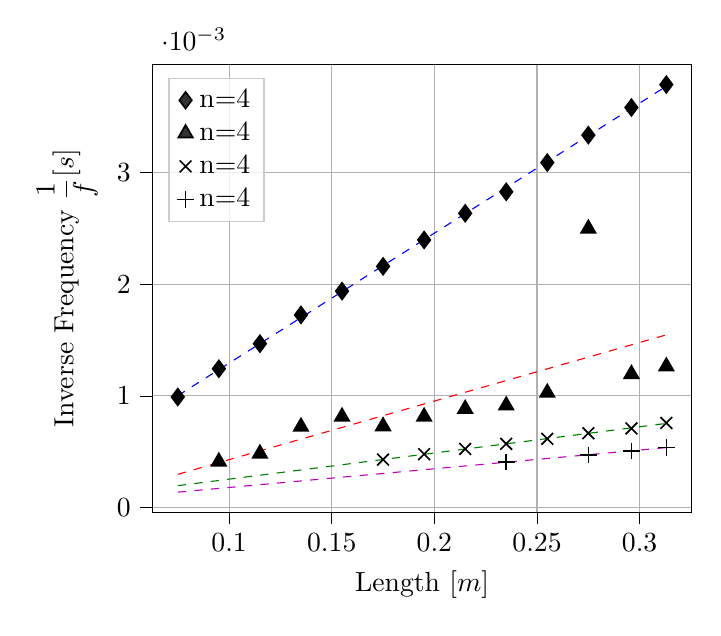
\begin{tikzpicture}

\definecolor{color0}{rgb}{0.75,0,0.75}

\begin{axis}[
legend cell align={left},
legend style={
  fill opacity=0.8,
  draw opacity=1,
  text opacity=1,
  at={(0.03,0.97)},
  anchor=north west,
  draw=white!80!black
},
tick align=outside,
tick pos=left,
x grid style={white!69.0196078431373!black},
xlabel={Length \(\displaystyle [m]\)},
xmajorgrids,
xmin=0.06255, xmax=0.32545,
xtick style={color=black},
y grid style={white!69.0196078431373!black},
ylabel={Inverse Frequency \(\displaystyle \frac{1}{f} [s]\)},
ymajorgrids,
ymin=-4.62327283096013e-05, ymax=0.00397150799436047,
ytick style={color=black}
]
\path [draw=black, semithick]
(axis cs:0.3125,0.00378888341605729)
--(axis cs:0.3135,0.00378888341605729);

\path [draw=black, semithick]
(axis cs:0.2955,0.00358320194926186)
--(axis cs:0.2965,0.00358320194926186);

\path [draw=black, semithick]
(axis cs:0.2745,0.00333600213504137)
--(axis cs:0.2755,0.00333600213504137);

\path [draw=black, semithick]
(axis cs:0.2545,0.00308966199097819)
--(axis cs:0.2555,0.00308966199097819);

\path [draw=black, semithick]
(axis cs:0.2345,0.00282805429864253)
--(axis cs:0.2355,0.00282805429864253);

\path [draw=black, semithick]
(axis cs:0.2145,0.00263532388130501)
--(axis cs:0.2155,0.00263532388130501);

\path [draw=black, semithick]
(axis cs:0.1945,0.00239647239263804)
--(axis cs:0.1955,0.00239647239263804);

\path [draw=black, semithick]
(axis cs:0.1745,0.00215978056629446)
--(axis cs:0.1755,0.00215978056629446);

\path [draw=black, semithick]
(axis cs:0.1545,0.00193764653451917)
--(axis cs:0.1555,0.00193764653451917);

\path [draw=black, semithick]
(axis cs:0.1345,0.00172476241397747)
--(axis cs:0.1355,0.00172476241397747);

\path [draw=black, semithick]
(axis cs:0.1145,0.00146679183290307)
--(axis cs:0.1155,0.00146679183290307);

\path [draw=black, semithick]
(axis cs:0.0945,0.00124251385402947)
--(axis cs:0.0955,0.00124251385402947);

\path [draw=black, semithick]
(axis cs:0.0745,0.000989276245498793)
--(axis cs:0.0755,0.000989276245498793);

\path [draw=black, semithick]
(axis cs:0.3125,0.00126272192337803)
--(axis cs:0.3135,0.00126272192337803);

\path [draw=black, semithick]
(axis cs:0.2955,0.00119441491585347)
--(axis cs:0.2965,0.00119441491585347);

\path [draw=black, semithick]
(axis cs:0.2745,0.00249744012387303)
--(axis cs:0.2755,0.00249744012387303);

\path [draw=black, semithick]
(axis cs:0.2545,0.00102711585866886)
--(axis cs:0.2555,0.00102711585866886);

\path [draw=black, semithick]
(axis cs:0.2345,0.000912991874372318)
--(axis cs:0.2355,0.000912991874372318);

\path [draw=black, semithick]
(axis cs:0.2145,0.000881888652738705)
--(axis cs:0.2155,0.000881888652738705);

\path [draw=black, semithick]
(axis cs:0.1945,0.000811938747340901)
--(axis cs:0.1955,0.000811938747340901);

\path [draw=black, semithick]
(axis cs:0.1745,0.000726733623057804)
--(axis cs:0.1755,0.000726733623057804);

\path [draw=black, semithick]
(axis cs:0.1545,0.000812162952374765)
--(axis cs:0.1555,0.000812162952374765);

\path [draw=black, semithick]
(axis cs:0.1345,0.000722381547485751)
--(axis cs:0.1355,0.000722381547485751);

\path [draw=black, semithick]
(axis cs:0.1145,0.000481225006376231)
--(axis cs:0.1155,0.000481225006376231);

\path [draw=black, semithick]
(axis cs:0.0945,0.000409223906860639)
--(axis cs:0.0955,0.000409223906860639);

\path [draw=black, semithick]
(axis cs:0.3125,0.000756675771998456)
--(axis cs:0.3135,0.000756675771998456);

\path [draw=black, semithick]
(axis cs:0.2955,0.000707603911634423)
--(axis cs:0.2965,0.000707603911634423);

\path [draw=black, semithick]
(axis cs:0.2745,0.00066459755295181)
--(axis cs:0.2755,0.00066459755295181);

\path [draw=black, semithick]
(axis cs:0.2545,0.000614409122746655)
--(axis cs:0.2555,0.000614409122746655);

\path [draw=black, semithick]
(axis cs:0.2345,0.000569570145411258)
--(axis cs:0.2355,0.000569570145411258);

\path [draw=black, semithick]
(axis cs:0.2145,0.000523716501783255)
--(axis cs:0.2155,0.000523716501783255);

\path [draw=black, semithick]
(axis cs:0.1945,0.000476987727105782)
--(axis cs:0.1955,0.000476987727105782);

\path [draw=black, semithick]
(axis cs:0.1745,0.000428096852631939)
--(axis cs:0.1755,0.000428096852631939);

\path [draw=black, semithick]
(axis cs:0.3125,0.00053656992310953)
--(axis cs:0.3135,0.00053656992310953);

\path [draw=black, semithick]
(axis cs:0.2955,0.000505998613563799)
--(axis cs:0.2965,0.000505998613563799);

\path [draw=black, semithick]
(axis cs:0.2745,0.000470745519679516)
--(axis cs:0.2755,0.000470745519679516);

\path [draw=black, semithick]
(axis cs:0.2345,0.000405278345167461)
--(axis cs:0.2355,0.000405278345167461);

\addplot [blue, dashed, forget plot]
table {%
0.0750000476837158 0.00100111961364746
0.312999963760376 0.00377404689788818
};
\addplot [red, dashed, forget plot]
table {%
0.0750000476837158 0.000296235084533691
0.312999963760376 0.00154590606689453
};
\addplot [green!50!black, dashed, forget plot]
table {%
0.0750000476837158 0.000194311141967773
0.312999963760376 0.000752449035644531
};
\addplot [color0, dashed, forget plot]
table {%
0.0750000476837158 0.000136375427246094
0.312999963760376 0.000535368919372559
};
\addplot [semithick, black, mark=diamond*, mark size=3, mark options={solid}, only marks]
table {%
0.312999963760376 0.00378882884979248
0.296000003814697 0.00358319282531738
0.274999976158142 0.00333595275878906
0.254999995231628 0.00308966636657715
0.235000014305115 0.00282800197601318
0.215000033378601 0.00263535976409912
0.194999933242798 0.00239646434783936
0.174999952316284 0.00215983390808105
0.154999971389771 0.0019376277923584
0.134999990463257 0.0017247200012207
0.115000009536743 0.00146675109863281
0.0950000286102295 0.00124251842498779
0.0750000476837158 0.000989317893981934
};
\addlegendentry{n=4}
\addplot [semithick, black, mark=triangle*, mark size=3, mark options={solid}, only marks]
table {%
0.312999963760376 0.00126266479492188
0.296000003814697 0.00119435787200928
0.274999976158142 0.00249743461608887
0.254999995231628 0.00102710723876953
0.235000014305115 0.000913023948669434
0.215000033378601 0.00088191032409668
0.194999933242798 0.000811934471130371
0.174999952316284 0.000726699829101562
0.154999971389771 0.000812172889709473
0.134999990463257 0.000722408294677734
0.115000009536743 0.000481247901916504
0.0950000286102295 0.000409245491027832
};
\addlegendentry{n=4}
\addplot [semithick, black, mark=x, mark size=3, mark options={solid}, only marks]
table {%
0.312999963760376 0.000756621360778809
0.296000003814697 0.000707626342773438
0.274999976158142 0.000664591789245605
0.254999995231628 0.000614404678344727
0.235000014305115 0.000569581985473633
0.215000033378601 0.000523686408996582
0.194999933242798 0.000476956367492676
0.174999952316284 0.000428080558776855
};
\addlegendentry{n=4}
\addplot [semithick, black, mark=+, mark size=3, mark options={solid}, only marks]
table {%
0.312999963760376 0.000536561012268066
0.296000003814697 0.000506043434143066
0.274999976158142 0.000470757484436035
0.235000014305115 0.000405311584472656
};
\addlegendentry{n=4}
\end{axis}

\end{tikzpicture}


    \caption{The relationship between the tube length and the inverse frequency}
    \label{fig:linplot}
\end{figure}

The linear best fit coefficients as well as the deviations, are given in table
\ref{tbl:fit-stats}.

\begin{table}[t!]
    \centering
    \caption{The Linear Fit Values}
    \label{tbl:fit-stats}
    \begin{tabular}{r | r r r r}
        \toprule
        \multirow{2}{*}{$n$} & \multirow{2}{*}{Slope $k$} & \multirow{2}{*}{y-intercept $c$} & \multicolumn{2}{c}{Fit Uncertainty} \\
        & & & $\sigma(k)$ & \sigma(c) \\
        \midrule
        1 & 1.17E-2 & 1.27E-4 & 5.76E-5 & 1.20E-5 \\
        2 & 5.25E-3 & -9.76E-5 & 1.70E-3 & 3.66E-4 \\
        3 & 2.34E-3 & 1.84E-5 & 2.28E-5 & 5.67E-6 \\
        4 & 1.68E-3 & 1.07E-5 & 2.27E-5 & 6.38E-6 \\
        \bottomrule
    \end{tabular}
\end{table}

For each value, the speed of sound $\nu$ was calculated according to:
\begin{equation}\label{eqn:soundspeed}
    \frac{4}{\nu \left(2n - 1\right)} = k
\end{equation}

These values are given in table \ref{tbl:soundspeed}.

\begin{table}[t!]
    \centering
    \caption{The Speed of sound calculated according to \eqref{eqn:soundspeed}}
    \label{tbl:soundspeed}
    \begin{tabular}{r | r r}
        \toprule
        $n$ & $\nu [\si{\frac{m}{s}}]$ & $\Delta \nu [\si{\frac{m}{s}}]$ \\
        \midrule
        1 & 343.32 & 1.70 \\
        2 & 253.93 & 81.98 \\
        3 & 341.08 & 3.31 \\
        4 & 340.85 & 4.61 \\
        \midrule
        $\bar{\nu}$ & \multicolumn{2}{c}{$319.80 \pm 91.6$} \\
        \bottomrule
    \end{tabular}
\end{table}

\section{Discussion}

In this section I discuss the processed data, considering possible sources of
error.

\subsection{Lack of Data Points for higher harmonics and lower tube lengths}

Some peaks are not available in table \ref{tbl:peaks}. This is due to the fact
that high frequency harmonics decay faster than lower frequency ones, implying
that at high frequencies the higher harmonics have small average amplitude.
This resulted in the Fourier transform not having peaks for higher harmonics,
resulting in a lack of data points.

\subsection{Outliers}

There is a clear outlier for $n=2$ at $l = 275\si{mm}$. This outlier is most
likely due to a systematic error -- either the microphone was tapped or some
external noise was present. I find it unlikely for this data point to be
attributed to statistical error as it is more than $5$ standard deviations away
from the mean.

Consequently, I believe this outlier should be considered as an irrelevant data
point.

\subsection{Qualitative statiscal analysis of harmonics and sources of error}

As Fig. \ref{fig:linplot} shows, the harmonics $n=1$, $n=3$ and $n=4$ fit very
neatly with a linear regression and, as table \ref{tbl:fit-stats} shows, the
square-root deviation from the linear fit is very small for these harmonics.

This leads me to believe the statistical error is very small for these
harmonics. That being said, the case of $n=4$ has very few data points, so,
care must be taken when drawing conclusions from it.

As for the case of $n=2$, besides the outlier, there is a higher statistical
uncertainty from table \ref{tbl:fit-stats}. The graph values also seem to deviate
more than for $n=1$, $n=3$, $n=4$. I believe this is due to these harmonics
being in midfrequency range, resulting in them being especially susceptible to
background noise. Furthermore, it is also important to note that blowing air
over the open end of the tube also created waveforms, which likely interacted
at this frequency.

\subsection{Relationship between tube length and wavelength}

As Fig. \ref{fig:linplot} shows, there is a clear linear relationship between
the tube length and the inverse of the frequency:
\begin{equation}
    \frac{1}{f} \propto L
\end{equation}
As given in table \ref{tbl:fit-stats}, the $k$ uncertainties are all under $2\%$,
except for $n=2$, indicating that each that point lies very close to the fit.
This, furthermore, indicates a strong correlation between the length and the
inverse frequency.

Since $1/f \propto \lambda$, this implies that:
\begin{equation}
    \lambda \propto L
\end{equation}

The values of the expected coefficients in \eqref{eqn:base-freq}:
\begin{align*}
    k(n=1) &= \frac{4}{\nu} = 1.17 \cdot 10^{-2} \\
    k(n=2) &= \frac{4}{3\nu} = 3.91 \cdot 10^{-3} \\
    k(n=3) &= \frac{4}{5\nu} = 2.35 \cdot 10^{-3} \\
    k(n=4) &= \frac{4}{7\nu} = 1.68 \cdot 10^{-3}
\end{align*}

Each $k$ was compared against the expected value and the results are given in
table \ref{tbl:coeffs}.

\begin{table}[t!]
    \centering
    \caption{The Slope Coefficients}
    \label{tbl:coeffs}
    \begin{tabular}{r | r r r}
        \toprule
        $n$ & $k_{expected}$ & $k_{actual}$ & $Z-score$ \\
        \midrule
        1 & 1.17E-2 & 1.17E-2 & 0 \\
        2 & 3.91E-3 & 5.25E-3 & 2.69 \\
        3 & 2.35E-3 & 2.34E-3 & -1.39 \\
        4 & 1.68E-3 & 1.68E-3 & 0 \\
        \bottomrule
    \end{tabular}
\end{table}

These Z-scores for $n \in {1, 3, 4}$ all give $>95\%$ statistical confidence in
the relationship between the inverse frequency and the tube length as the one
predicted. Consequently, this implies that \eqref{eqn:base-freq} holds.

The case of $n=2$ has a high Z-score, but, as previously discussed, I believe
it is an outlier.

This gives me confidence in stating that the relationship in \eqref{eqn:base}
holds.

\subsection{The Speed of Sound}

The mean speed of sound across all the harmonics was calculated to be:
\begin{equation}
    \nu_1 = (319.80 \pm 91.6) \si{\frac{m}{s}}
\end{equation}

However, table \ref{tbl:soundspeed} possibly indicates that this may not be the
correct method in calculating the speed of sound.  As previously discussed, the
case of $n=2$ had a severe outlier. This outlier propagates up to the
calculation for the speed of sound, as table \ref{tbl:soundspeed} shows.
Furthermore, the extremely high uncertainty of $32.28\%$ for the wavespeed of
the $n=2$ case leads me to believe that it is a useless datapoint in evaluating
the actual speed of sound.

Disregarding the $n=2$ case, the mean speed is:
\begin{equation*}
    \nu_2 = (341.75 \pm 9.62) \si{\frac{m}{s}}
\end{equation*}

This value has much tighter uncertainty and, I believe, is closer to the true
one.

The expected speed of sound was:
\begin{equation*}
    \nu_{ex} = 340.8 \si{\frac{m}{s}}
\end{equation*}

The Z-score for $\nu_1$ is:
\begin{equation*}
    Z_1 = -0.46
\end{equation*}

The Z-score for $\nu_2$ is:
\begin{equation*}
    Z_1 = 0.17
\end{equation*}

These small values indicate that both values are correct. That being said, the
reader must be careful in noting the huge uncertainty for $\nu_1$ and $\nu_2$
being in the range of $\nu_1 + \Delta \nu_1$.

I believe that $\nu_2$ is the more reasonable measurement and should be the
considered.

\section{Conclusion}

To conclude, this research appears to indicate, with $>95\%$ statistical
certainty that \eqref{eqn:base} holds. Furthermore, the speed of sound was
identified to be:
\begin{equation*}
    \nu = (341.75 \pm 9.62) \si{\frac{m}{s}}
\end{equation*}

\begin{thebibliography}{00}
    \bibitem{audacity} Audacity® software is copyright © 1999-2021 Audacity
    Team. The name Audacity® is a registered trademark.
    \bibitem{at2021} Audio Technica, \textit{AT2021}. [Online]. Available:
    \url{https://www.audio-technica.com/en-us/at2021}. [Accessed: 15-Mar-2021]. 
    \bibitem{numpy} Charles R. Harris, K. Jarrod Millman, Stefan J. van der
    Walt, Ralf Gommers, Pauli Virtanen, David Cournapeau, Eric Wieser, Julian
    Taylor, Sebastian Berg, Nathaniel J. Smith, Robert Kern, Matti Picus,
    Stephan Hoyer, Marten H. van Kerkwijk, Matthew Brett, Allan Haldane, Jaime
    Fernández del Río, Mark Wiebe, Pearu Peterson, Pierre Gérard-Marchant,
    Kevin Sheppard, Tyler Reddy, Warren Weckesser, Hameer Abbasi, Christoph
    Gohlke \& Travis E. Oliphant. \textit{Array programming with NumPy},
    Nature, 585, 357–362 (2020), DOI:10.1038/s41586-020- 2649-2
    \bibitem{matplotlib} J. D. Hunter, \textit{Matplotlib: A 2D Graphics
    Environment}, Computing in Science \& Engineering, vol. 9, no. 3, pp.
    90-95, 2007.
    \bibitem{scipy} Pauli Virtanen, Ralf Gommers, Travis E. Oliphant, Matt
    Haberland, Tyler Reddy, David Cournapeau, Evgeni Burovski, Pearu Peterson,
    Warren Weckesser, Jonathan Bright, Stéfan J. van der Walt, Matthew Brett,
    Joshua Wilson, K. Jarrod Millman, Nikolay Mayorov, Andrew R. J. Nelson,
    Eric Jones, Robert Kern, Eric Larson, CJ Carey, İlhan Polat, Yu Feng, Eric
    W. Moore, Jake VanderPlas, Denis Laxalde, Josef Perktold, Robert Cimrman,
    Ian Henriksen, E.A. Quintero, Charles R Harris, Anne M. Archibald, Antônio
    H. Ribeiro, Fabian Pedregosa, Paul van Mulbregt, and SciPy 1.0
    Contributors. (2020) ''SciPy 1.0: Fundamental Algorithms for Scientific
    Computing in Python``. \textit{Nature Methods}, 17(3), 261-272
    \bibitem{python} Python Software Foundation, \textit{Python Language
    Reference}, version 3.9.  Available: http://www.python.org.
    \bibitem{focusrite} ``Scarlett Solo,'' \textit{Focusrite}. [Online].
    Available:
    \url{https://focusrite.com/en/usb-audio-interface/scarlett/scarlett-solo}.
    [Accessed: 15-Mar-2021]. 
    \bibitem{sostbl} ``Velocity of Sound in Air,'' \textit{Engineering
    ToolBox}. [Online].  Available:
    \url{https://www.engineeringtoolbox.com/air-speed-sound-d_603.html}.
    [Accessed: 15-Mar-2021]. 
    \bibitem{raw-waveforms}
    \url{https://github.com/markovejnovic/tube-harmonics}
\end{thebibliography}

\end{document}
